\documentclass[twoside]{book}

% Packages required by doxygen
\usepackage{calc}
\usepackage{doxygen}
\usepackage{graphicx}
\usepackage[utf8]{inputenc}
\usepackage{makeidx}
\usepackage{multicol}
\usepackage{multirow}
\usepackage{textcomp}
\usepackage[table]{xcolor}

% Font selection
\usepackage[T1]{fontenc}
\usepackage{mathptmx}
\usepackage[scaled=.90]{helvet}
\usepackage{courier}
\usepackage{amssymb}
\usepackage{sectsty}
\renewcommand{\familydefault}{\sfdefault}
\allsectionsfont{%
  \fontseries{bc}\selectfont%
  \color{darkgray}%
}
\renewcommand{\DoxyLabelFont}{%
  \fontseries{bc}\selectfont%
  \color{darkgray}%
}

% Page & text layout
\usepackage{geometry}
\geometry{%
  a4paper,%
  top=2.5cm,%
  bottom=2.5cm,%
  left=2.5cm,%
  right=2.5cm%
}
\tolerance=750
\hfuzz=15pt
\hbadness=750
\setlength{\emergencystretch}{15pt}
\setlength{\parindent}{0cm}
\setlength{\parskip}{0.2cm}
\makeatletter
\renewcommand{\paragraph}{%
  \@startsection{paragraph}{4}{0ex}{-1.0ex}{1.0ex}{%
    \normalfont\normalsize\bfseries\SS@parafont%
  }%
}
\renewcommand{\subparagraph}{%
  \@startsection{subparagraph}{5}{0ex}{-1.0ex}{1.0ex}{%
    \normalfont\normalsize\bfseries\SS@subparafont%
  }%
}
\makeatother

% Headers & footers
\usepackage{fancyhdr}
\pagestyle{fancyplain}
\fancyhead[LE]{\fancyplain{}{\bfseries\thepage}}
\fancyhead[CE]{\fancyplain{}{}}
\fancyhead[RE]{\fancyplain{}{\bfseries\leftmark}}
\fancyhead[LO]{\fancyplain{}{\bfseries\rightmark}}
\fancyhead[CO]{\fancyplain{}{}}
\fancyhead[RO]{\fancyplain{}{\bfseries\thepage}}
\fancyfoot[LE]{\fancyplain{}{}}
\fancyfoot[CE]{\fancyplain{}{}}
\fancyfoot[RE]{\fancyplain{}{\bfseries\scriptsize Generated on Mon Sep 17 2018 12\-:15\-:03 for M\-A\-L\-O\-N\-E by Doxygen }}
\fancyfoot[LO]{\fancyplain{}{\bfseries\scriptsize Generated on Mon Sep 17 2018 12\-:15\-:03 for M\-A\-L\-O\-N\-E by Doxygen }}
\fancyfoot[CO]{\fancyplain{}{}}
\fancyfoot[RO]{\fancyplain{}{}}
\renewcommand{\footrulewidth}{0.4pt}
\renewcommand{\chaptermark}[1]{%
  \markboth{#1}{}%
}
\renewcommand{\sectionmark}[1]{%
  \markright{\thesection\ #1}%
}

% Indices & bibliography
\usepackage{natbib}
\usepackage[titles]{tocloft}
\setcounter{tocdepth}{3}
\setcounter{secnumdepth}{5}
\makeindex

% Hyperlinks (required, but should be loaded last)
\usepackage{ifpdf}
\ifpdf
  \usepackage[pdftex,pagebackref=true]{hyperref}
\else
  \usepackage[ps2pdf,pagebackref=true]{hyperref}
\fi
\hypersetup{%
  colorlinks=true,%
  linkcolor=blue,%
  citecolor=blue,%
  unicode%
}

% Custom commands
\newcommand{\clearemptydoublepage}{%
  \newpage{\pagestyle{empty}\cleardoublepage}%
}


%===== C O N T E N T S =====

\begin{document}

% Titlepage & ToC
\hypersetup{pageanchor=false}
\pagenumbering{roman}
\begin{titlepage}
\vspace*{7cm}
\begin{center}%
{\Large M\-A\-L\-O\-N\-E }\\
\vspace*{1cm}
{\large Generated by Doxygen 1.8.6}\\
\vspace*{0.5cm}
{\small Mon Sep 17 2018 12:15:03}\\
\end{center}
\end{titlepage}
\clearemptydoublepage
\tableofcontents
\clearemptydoublepage
\pagenumbering{arabic}
\hypersetup{pageanchor=true}

%--- Begin generated contents ---
\chapter{Data Structure Index}
\section{Data Structures}
Here are the data structures with brief descriptions\-:\begin{DoxyCompactList}
\item\contentsline{section}{\hyperlink{struct__cell}{\-\_\-cell} }{\pageref{struct__cell}}{}
\item\contentsline{section}{\hyperlink{struct__test}{\-\_\-test} }{\pageref{struct__test}}{}
\item\contentsline{section}{\hyperlink{structMutantList}{Mutant\-List} }{\pageref{structMutantList}}{}
\item\contentsline{section}{\hyperlink{structT__stConfigValues}{T\-\_\-st\-Config\-Values} }{\pageref{structT__stConfigValues}}{}
\item\contentsline{section}{\hyperlink{structT__stEquivalentInfo}{T\-\_\-st\-Equivalent\-Info} }{\pageref{structT__stEquivalentInfo}}{}
\item\contentsline{section}{\hyperlink{structT__stExecutionMap}{T\-\_\-st\-Execution\-Map} }{\pageref{structT__stExecutionMap}}{}
\item\contentsline{section}{\hyperlink{structT__stExecutionStructure}{T\-\_\-st\-Execution\-Structure} }{\pageref{structT__stExecutionStructure}}{}
\item\contentsline{section}{\hyperlink{structT__stIniValues}{T\-\_\-st\-Ini\-Values} }{\pageref{structT__stIniValues}}{}
\item\contentsline{section}{\hyperlink{structT__stM}{T\-\_\-st\-M} }{\pageref{structT__stM}}{}
\item\contentsline{section}{\hyperlink{structT__stMutant}{T\-\_\-st\-Mutant} }{\pageref{structT__stMutant}}{}
\item\contentsline{section}{\hyperlink{structT__stMutantExecution}{T\-\_\-st\-Mutant\-Execution} }{\pageref{structT__stMutantExecution}}{}
\item\contentsline{section}{\hyperlink{structT__stTestInfo}{T\-\_\-st\-Test\-Info} }{\pageref{structT__stTestInfo}}{}
\item\contentsline{section}{\hyperlink{structT__stTestList}{T\-\_\-st\-Test\-List} }{\pageref{structT__stTestList}}{}
\item\contentsline{section}{\hyperlink{structT__stTI}{T\-\_\-st\-T\-I} }{\pageref{structT__stTI}}{}
\item\contentsline{section}{\hyperlink{structVector}{Vector} }{\pageref{structVector}}{}
\end{DoxyCompactList}

\chapter{File Index}
\section{File List}
Here is a list of all files with brief descriptions\-:\begin{DoxyCompactList}
\item\contentsline{section}{\hyperlink{_8dep_8inc}{.\-dep.\-inc} }{\pageref{_8dep_8inc}}{}
\item\contentsline{section}{\hyperlink{Auxiliars_8c}{Auxiliars.\-c} }{\pageref{Auxiliars_8c}}{}
\item\contentsline{section}{\hyperlink{Auxiliars_8h}{Auxiliars.\-h} }{\pageref{Auxiliars_8h}}{}
\item\contentsline{section}{\hyperlink{configuration_8c}{configuration.\-c} }{\pageref{configuration_8c}}{}
\item\contentsline{section}{\hyperlink{configuration_8h}{configuration.\-h} }{\pageref{configuration_8h}}{}
\item\contentsline{section}{\hyperlink{debugMode_8c}{debug\-Mode.\-c} }{\pageref{debugMode_8c}}{}
\item\contentsline{section}{\hyperlink{debugMode_8h}{debug\-Mode.\-h} }{\pageref{debugMode_8h}}{}
\item\contentsline{section}{\hyperlink{distribution__adaptive__grain_8c}{distribution\-\_\-adaptive\-\_\-grain.\-c} }{\pageref{distribution__adaptive__grain_8c}}{}
\item\contentsline{section}{\hyperlink{distribution__dynamic__mutants_8c}{distribution\-\_\-dynamic\-\_\-mutants.\-c} }{\pageref{distribution__dynamic__mutants_8c}}{}
\item\contentsline{section}{\hyperlink{distribution__full__dynamic_8c}{distribution\-\_\-full\-\_\-dynamic.\-c} }{\pageref{distribution__full__dynamic_8c}}{}
\item\contentsline{section}{\hyperlink{distribution__full__dynamic__scatter_8c}{distribution\-\_\-full\-\_\-dynamic\-\_\-scatter.\-c} }{\pageref{distribution__full__dynamic__scatter_8c}}{}
\item\contentsline{section}{\hyperlink{distribution__static__mutants_8c}{distribution\-\_\-static\-\_\-mutants.\-c} }{\pageref{distribution__static__mutants_8c}}{}
\item\contentsline{section}{\hyperlink{DistributionAlgorithms_8c}{Distribution\-Algorithms.\-c} }{\pageref{DistributionAlgorithms_8c}}{}
\item\contentsline{section}{\hyperlink{DistributionAlgorithms_8h}{Distribution\-Algorithms.\-h} }{\pageref{DistributionAlgorithms_8h}}{}
\item\contentsline{section}{\hyperlink{EnvFileSend_8c}{Env\-File\-Send.\-c} }{\pageref{EnvFileSend_8c}}{}
\item\contentsline{section}{\hyperlink{EnvFileSend_8h}{Env\-File\-Send.\-h} }{\pageref{EnvFileSend_8h}}{}
\item\contentsline{section}{\hyperlink{EquivalenceChecking_8c}{Equivalence\-Checking.\-c} }{\pageref{EquivalenceChecking_8c}}{}
\item\contentsline{section}{\hyperlink{EquivalenceChecking_8h}{Equivalence\-Checking.\-h} }{\pageref{EquivalenceChecking_8h}}{}
\item\contentsline{section}{\hyperlink{ExecutionMapSaver_8c}{Execution\-Map\-Saver.\-c} }{\pageref{ExecutionMapSaver_8c}}{}
\item\contentsline{section}{\hyperlink{ExecutionMapSaver_8h}{Execution\-Map\-Saver.\-h} }{\pageref{ExecutionMapSaver_8h}}{}
\item\contentsline{section}{\hyperlink{executionMode_8c}{execution\-Mode.\-c} }{\pageref{executionMode_8c}}{}
\item\contentsline{section}{\hyperlink{executionMode_8h}{execution\-Mode.\-h} }{\pageref{executionMode_8h}}{}
\item\contentsline{section}{\hyperlink{kvec_8h}{kvec.\-h} }{\pageref{kvec_8h}}{}
\item\contentsline{section}{\hyperlink{main_8c}{main.\-c} }{\pageref{main_8c}}{}
\item\contentsline{section}{\hyperlink{Malone_8c}{Malone.\-c} }{\pageref{Malone_8c}}{}
\item\contentsline{section}{\hyperlink{Malone_8h}{Malone.\-h} }{\pageref{Malone_8h}}{}
\item\contentsline{section}{\hyperlink{MonteCarlo_8c}{Monte\-Carlo.\-c} }{\pageref{MonteCarlo_8c}}{}
\item\contentsline{section}{\hyperlink{MonteCarlo_8h}{Monte\-Carlo.\-h} }{\pageref{MonteCarlo_8h}}{}
\item\contentsline{section}{\hyperlink{MPI__Operations_8c}{M\-P\-I\-\_\-\-Operations.\-c} }{\pageref{MPI__Operations_8c}}{}
\item\contentsline{section}{\hyperlink{MPI__Operations_8h}{M\-P\-I\-\_\-\-Operations.\-h} }{\pageref{MPI__Operations_8h}}{}
\item\contentsline{section}{\hyperlink{MPIDataTypes_8c}{M\-P\-I\-Data\-Types.\-c} }{\pageref{MPIDataTypes_8c}}{}
\item\contentsline{section}{\hyperlink{MPIDataTypes_8h}{M\-P\-I\-Data\-Types.\-h} }{\pageref{MPIDataTypes_8h}}{}
\item\contentsline{section}{\hyperlink{Options_8h}{Options.\-h} }{\pageref{Options_8h}}{}
\item\contentsline{section}{\hyperlink{PiReduce_8c}{Pi\-Reduce.\-c} }{\pageref{PiReduce_8c}}{}
\item\contentsline{section}{\hyperlink{printers_8c}{printers.\-c} }{\pageref{printers_8c}}{}
\item\contentsline{section}{\hyperlink{printers_8h}{printers.\-h} }{\pageref{printers_8h}}{}
\item\contentsline{section}{\hyperlink{randomElements_8c}{random\-Elements.\-c} }{\pageref{randomElements_8c}}{}
\item\contentsline{section}{\hyperlink{randomElements_8h}{random\-Elements.\-h} }{\pageref{randomElements_8h}}{}
\item\contentsline{section}{\hyperlink{tests_8c}{tests.\-c} }{\pageref{tests_8c}}{}
\item\contentsline{section}{\hyperlink{tests_8h}{tests.\-h} }{\pageref{tests_8h}}{}
\item\contentsline{section}{\hyperlink{testVec_8c}{test\-Vec.\-c} }{\pageref{testVec_8c}}{}
\item\contentsline{section}{\hyperlink{transformations_8c}{transformations.\-c} }{\pageref{transformations_8c}}{}
\item\contentsline{section}{\hyperlink{transformations_8h}{transformations.\-h} }{\pageref{transformations_8h}}{}
\item\contentsline{section}{\hyperlink{Vector_8h}{Vector.\-h} }{\pageref{Vector_8h}}{}
\end{DoxyCompactList}

\chapter{Data Structure Documentation}
\hypertarget{struct__cell}{\section{\-\_\-cell Struct Reference}
\label{struct__cell}\index{\-\_\-cell@{\-\_\-cell}}
}
\subsection*{Data Fields}
\begin{DoxyCompactItemize}
\item 
int \hyperlink{struct__cell_a9be272aa3ca6654d85231bcd3590f3d8}{coord} \mbox{[}2\mbox{]}
\item 
double \hyperlink{struct__cell_a705a2494c30f912d5ceff1338193c5a9}{elevation}
\item 
char \hyperlink{struct__cell_a9b25becd5439e9ad849c5e95361478ad}{landcover}
\item 
double \hyperlink{struct__cell_adeb26be20eaf77e2e32a470ee357e82c}{albedos} \mbox{[}4\mbox{]}
\end{DoxyCompactItemize}


\subsection{Field Documentation}
\hypertarget{struct__cell_adeb26be20eaf77e2e32a470ee357e82c}{\index{\-\_\-cell@{\-\_\-cell}!albedos@{albedos}}
\index{albedos@{albedos}!_cell@{\-\_\-cell}}
\subsubsection[{albedos}]{\setlength{\rightskip}{0pt plus 5cm}double \-\_\-cell\-::albedos\mbox{[}4\mbox{]}}}\label{struct__cell_adeb26be20eaf77e2e32a470ee357e82c}
\hypertarget{struct__cell_a9be272aa3ca6654d85231bcd3590f3d8}{\index{\-\_\-cell@{\-\_\-cell}!coord@{coord}}
\index{coord@{coord}!_cell@{\-\_\-cell}}
\subsubsection[{coord}]{\setlength{\rightskip}{0pt plus 5cm}int \-\_\-cell\-::coord\mbox{[}2\mbox{]}}}\label{struct__cell_a9be272aa3ca6654d85231bcd3590f3d8}
\hypertarget{struct__cell_a705a2494c30f912d5ceff1338193c5a9}{\index{\-\_\-cell@{\-\_\-cell}!elevation@{elevation}}
\index{elevation@{elevation}!_cell@{\-\_\-cell}}
\subsubsection[{elevation}]{\setlength{\rightskip}{0pt plus 5cm}double \-\_\-cell\-::elevation}}\label{struct__cell_a705a2494c30f912d5ceff1338193c5a9}
\hypertarget{struct__cell_a9b25becd5439e9ad849c5e95361478ad}{\index{\-\_\-cell@{\-\_\-cell}!landcover@{landcover}}
\index{landcover@{landcover}!_cell@{\-\_\-cell}}
\subsubsection[{landcover}]{\setlength{\rightskip}{0pt plus 5cm}char \-\_\-cell\-::landcover}}\label{struct__cell_a9b25becd5439e9ad849c5e95361478ad}


The documentation for this struct was generated from the following file\-:\begin{DoxyCompactItemize}
\item 
\hyperlink{MPIDataTypes_8c}{M\-P\-I\-Data\-Types.\-c}\end{DoxyCompactItemize}

\hypertarget{struct__test}{\section{\-\_\-test Struct Reference}
\label{struct__test}\index{\-\_\-test@{\-\_\-test}}
}
\subsection*{Data Fields}
\begin{DoxyCompactItemize}
\item 
char \hyperlink{struct__test_ab4ddbda022cf86dfad1c7405feb8acdf}{landcover}
\item 
int \hyperlink{struct__test_a8a75ad7b07875699f2e56a0cfba90015}{coord}
\item 
double \hyperlink{struct__test_a304d9c5eb29e37799d2912f092b75db4}{elevation}
\end{DoxyCompactItemize}


\subsection{Field Documentation}
\hypertarget{struct__test_a8a75ad7b07875699f2e56a0cfba90015}{\index{\-\_\-test@{\-\_\-test}!coord@{coord}}
\index{coord@{coord}!_test@{\-\_\-test}}
\subsubsection[{coord}]{\setlength{\rightskip}{0pt plus 5cm}int \-\_\-test\-::coord}}\label{struct__test_a8a75ad7b07875699f2e56a0cfba90015}
\hypertarget{struct__test_a304d9c5eb29e37799d2912f092b75db4}{\index{\-\_\-test@{\-\_\-test}!elevation@{elevation}}
\index{elevation@{elevation}!_test@{\-\_\-test}}
\subsubsection[{elevation}]{\setlength{\rightskip}{0pt plus 5cm}double \-\_\-test\-::elevation}}\label{struct__test_a304d9c5eb29e37799d2912f092b75db4}
\hypertarget{struct__test_ab4ddbda022cf86dfad1c7405feb8acdf}{\index{\-\_\-test@{\-\_\-test}!landcover@{landcover}}
\index{landcover@{landcover}!_test@{\-\_\-test}}
\subsubsection[{landcover}]{\setlength{\rightskip}{0pt plus 5cm}char \-\_\-test\-::landcover}}\label{struct__test_ab4ddbda022cf86dfad1c7405feb8acdf}


The documentation for this struct was generated from the following file\-:\begin{DoxyCompactItemize}
\item 
\hyperlink{MPIDataTypes_8c}{M\-P\-I\-Data\-Types.\-c}\end{DoxyCompactItemize}

\hypertarget{structMutantList}{\section{Mutant\-List Struct Reference}
\label{structMutantList}\index{Mutant\-List@{Mutant\-List}}
}


{\ttfamily \#include $<$Options.\-h$>$}



Collaboration diagram for Mutant\-List\-:\nopagebreak
\begin{figure}[H]
\begin{center}
\leavevmode
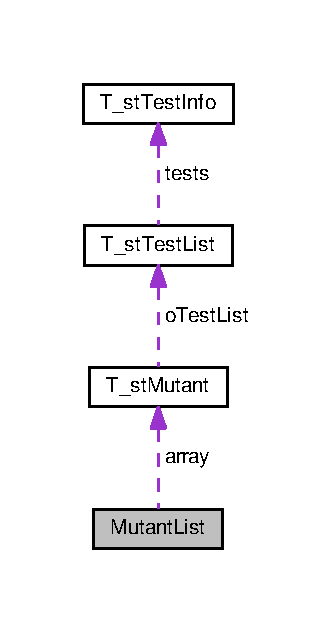
\includegraphics[width=160pt]{structMutantList__coll__graph}
\end{center}
\end{figure}
\subsection*{Data Fields}
\begin{DoxyCompactItemize}
\item 
int \hyperlink{structMutantList_abfe5da02681fadfbc5c85c150a880508}{n\-Elems}
\item 
int \hyperlink{structMutantList_a0238362172eaecea60b5cc88e4406f8f}{n\-Max}
\item 
int \hyperlink{structMutantList_a52c03779cb04c5d8a5344c70e5e39b89}{n\-Dead}
\item 
double \hyperlink{structMutantList_a43fbe4e680f5b4d1f4c001f793d2aa40}{d\-Time}
\item 
\hyperlink{structT__stMutant}{T\-\_\-st\-Mutant} $\ast$ \hyperlink{structMutantList_a880314b02f26bbaebb4277d514f6d9de}{array} \mbox{[}\hyperlink{Options_8h_a7b5fa9fc08e6e43e329c804ac562bd00}{M\-A\-X\-\_\-\-M\-U\-T\-A\-N\-T\-S}\mbox{]}
\end{DoxyCompactItemize}


\subsection{Field Documentation}
\hypertarget{structMutantList_a880314b02f26bbaebb4277d514f6d9de}{\index{Mutant\-List@{Mutant\-List}!array@{array}}
\index{array@{array}!MutantList@{Mutant\-List}}
\subsubsection[{array}]{\setlength{\rightskip}{0pt plus 5cm}{\bf T\-\_\-st\-Mutant}$\ast$ Mutant\-List\-::array\mbox{[}{\bf M\-A\-X\-\_\-\-M\-U\-T\-A\-N\-T\-S}\mbox{]}}}\label{structMutantList_a880314b02f26bbaebb4277d514f6d9de}
\hypertarget{structMutantList_a43fbe4e680f5b4d1f4c001f793d2aa40}{\index{Mutant\-List@{Mutant\-List}!d\-Time@{d\-Time}}
\index{d\-Time@{d\-Time}!MutantList@{Mutant\-List}}
\subsubsection[{d\-Time}]{\setlength{\rightskip}{0pt plus 5cm}double Mutant\-List\-::d\-Time}}\label{structMutantList_a43fbe4e680f5b4d1f4c001f793d2aa40}
\hypertarget{structMutantList_a52c03779cb04c5d8a5344c70e5e39b89}{\index{Mutant\-List@{Mutant\-List}!n\-Dead@{n\-Dead}}
\index{n\-Dead@{n\-Dead}!MutantList@{Mutant\-List}}
\subsubsection[{n\-Dead}]{\setlength{\rightskip}{0pt plus 5cm}int Mutant\-List\-::n\-Dead}}\label{structMutantList_a52c03779cb04c5d8a5344c70e5e39b89}
\hypertarget{structMutantList_abfe5da02681fadfbc5c85c150a880508}{\index{Mutant\-List@{Mutant\-List}!n\-Elems@{n\-Elems}}
\index{n\-Elems@{n\-Elems}!MutantList@{Mutant\-List}}
\subsubsection[{n\-Elems}]{\setlength{\rightskip}{0pt plus 5cm}int Mutant\-List\-::n\-Elems}}\label{structMutantList_abfe5da02681fadfbc5c85c150a880508}
\hypertarget{structMutantList_a0238362172eaecea60b5cc88e4406f8f}{\index{Mutant\-List@{Mutant\-List}!n\-Max@{n\-Max}}
\index{n\-Max@{n\-Max}!MutantList@{Mutant\-List}}
\subsubsection[{n\-Max}]{\setlength{\rightskip}{0pt plus 5cm}int Mutant\-List\-::n\-Max}}\label{structMutantList_a0238362172eaecea60b5cc88e4406f8f}


The documentation for this struct was generated from the following file\-:\begin{DoxyCompactItemize}
\item 
\hyperlink{Options_8h}{Options.\-h}\end{DoxyCompactItemize}

\hypertarget{structT__stConfigValues}{\section{T\-\_\-st\-Config\-Values Struct Reference}
\label{structT__stConfigValues}\index{T\-\_\-st\-Config\-Values@{T\-\_\-st\-Config\-Values}}
}


{\ttfamily \#include $<$configuration.\-h$>$}

\subsection*{Data Fields}
\begin{DoxyCompactItemize}
\item 
int \hyperlink{structT__stConfigValues_a24bdee712ac9ec8ea098475833bf64c7}{n\-Debug\-Main\-Master}
\item 
int \hyperlink{structT__stConfigValues_ad0b0917ce95d25b3fefcd85bdf0d9d72}{n\-Debug\-Main\-Workers}
\item 
int \hyperlink{structT__stConfigValues_a2505593b064dfec1b1f25c0c241d53d9}{n\-Debug\-Mpi\-Ops}
\item 
int \hyperlink{structT__stConfigValues_a617bb7970be5be3996acc27fe37b736e}{n\-Debug\-Aux}
\item 
int \hyperlink{structT__stConfigValues_a09bbefde23de1f9ee642e17f030db9e5}{n\-Debug\-Dist\-Master}
\item 
int \hyperlink{structT__stConfigValues_a177845357bb706165cd4a3dc1ffdbdcc}{n\-Debug\-Dist\-Workers}
\item 
int \hyperlink{structT__stConfigValues_af872d01e2b82875a270909cd7e59dfc6}{n\-Debug\-Dist\-Common}
\item 
int \hyperlink{structT__stConfigValues_a317e5fcb75d03f261b71e58a02ba52d5}{n\-Debug\-Dist\-Updates}
\item 
int \hyperlink{structT__stConfigValues_aea4fadbdb4e6c659f119d38a806c38c2}{n\-Debug\-Printers}
\item 
int \hyperlink{structT__stConfigValues_ad00796e06901e3a43852c48a2413dc11}{n\-Debug\-Execution\-Mode}
\item 
int \hyperlink{structT__stConfigValues_acda2f735f20ed7d850b1f1a4038b778a}{n\-Debug\-Trans}
\item 
int \hyperlink{structT__stConfigValues_ad1b2105aee0a657c0e68c4db0c75b4d6}{n\-Debug\-Main\-Command}
\item 
int \hyperlink{structT__stConfigValues_ab9d02864b458c46d840f7e783ebafb95}{n\-Debug\-Config}
\item 
char $\ast$ \hyperlink{structT__stConfigValues_a1d061110525c304ae6caa537fa72c263}{str\-Results\-File}
\end{DoxyCompactItemize}


\subsection{Field Documentation}
\hypertarget{structT__stConfigValues_a617bb7970be5be3996acc27fe37b736e}{\index{T\-\_\-st\-Config\-Values@{T\-\_\-st\-Config\-Values}!n\-Debug\-Aux@{n\-Debug\-Aux}}
\index{n\-Debug\-Aux@{n\-Debug\-Aux}!T_stConfigValues@{T\-\_\-st\-Config\-Values}}
\subsubsection[{n\-Debug\-Aux}]{\setlength{\rightskip}{0pt plus 5cm}int T\-\_\-st\-Config\-Values\-::n\-Debug\-Aux}}\label{structT__stConfigValues_a617bb7970be5be3996acc27fe37b736e}
\hypertarget{structT__stConfigValues_ab9d02864b458c46d840f7e783ebafb95}{\index{T\-\_\-st\-Config\-Values@{T\-\_\-st\-Config\-Values}!n\-Debug\-Config@{n\-Debug\-Config}}
\index{n\-Debug\-Config@{n\-Debug\-Config}!T_stConfigValues@{T\-\_\-st\-Config\-Values}}
\subsubsection[{n\-Debug\-Config}]{\setlength{\rightskip}{0pt plus 5cm}int T\-\_\-st\-Config\-Values\-::n\-Debug\-Config}}\label{structT__stConfigValues_ab9d02864b458c46d840f7e783ebafb95}
\hypertarget{structT__stConfigValues_af872d01e2b82875a270909cd7e59dfc6}{\index{T\-\_\-st\-Config\-Values@{T\-\_\-st\-Config\-Values}!n\-Debug\-Dist\-Common@{n\-Debug\-Dist\-Common}}
\index{n\-Debug\-Dist\-Common@{n\-Debug\-Dist\-Common}!T_stConfigValues@{T\-\_\-st\-Config\-Values}}
\subsubsection[{n\-Debug\-Dist\-Common}]{\setlength{\rightskip}{0pt plus 5cm}int T\-\_\-st\-Config\-Values\-::n\-Debug\-Dist\-Common}}\label{structT__stConfigValues_af872d01e2b82875a270909cd7e59dfc6}
\hypertarget{structT__stConfigValues_a09bbefde23de1f9ee642e17f030db9e5}{\index{T\-\_\-st\-Config\-Values@{T\-\_\-st\-Config\-Values}!n\-Debug\-Dist\-Master@{n\-Debug\-Dist\-Master}}
\index{n\-Debug\-Dist\-Master@{n\-Debug\-Dist\-Master}!T_stConfigValues@{T\-\_\-st\-Config\-Values}}
\subsubsection[{n\-Debug\-Dist\-Master}]{\setlength{\rightskip}{0pt plus 5cm}int T\-\_\-st\-Config\-Values\-::n\-Debug\-Dist\-Master}}\label{structT__stConfigValues_a09bbefde23de1f9ee642e17f030db9e5}
\hypertarget{structT__stConfigValues_a317e5fcb75d03f261b71e58a02ba52d5}{\index{T\-\_\-st\-Config\-Values@{T\-\_\-st\-Config\-Values}!n\-Debug\-Dist\-Updates@{n\-Debug\-Dist\-Updates}}
\index{n\-Debug\-Dist\-Updates@{n\-Debug\-Dist\-Updates}!T_stConfigValues@{T\-\_\-st\-Config\-Values}}
\subsubsection[{n\-Debug\-Dist\-Updates}]{\setlength{\rightskip}{0pt plus 5cm}int T\-\_\-st\-Config\-Values\-::n\-Debug\-Dist\-Updates}}\label{structT__stConfigValues_a317e5fcb75d03f261b71e58a02ba52d5}
\hypertarget{structT__stConfigValues_a177845357bb706165cd4a3dc1ffdbdcc}{\index{T\-\_\-st\-Config\-Values@{T\-\_\-st\-Config\-Values}!n\-Debug\-Dist\-Workers@{n\-Debug\-Dist\-Workers}}
\index{n\-Debug\-Dist\-Workers@{n\-Debug\-Dist\-Workers}!T_stConfigValues@{T\-\_\-st\-Config\-Values}}
\subsubsection[{n\-Debug\-Dist\-Workers}]{\setlength{\rightskip}{0pt plus 5cm}int T\-\_\-st\-Config\-Values\-::n\-Debug\-Dist\-Workers}}\label{structT__stConfigValues_a177845357bb706165cd4a3dc1ffdbdcc}
\hypertarget{structT__stConfigValues_ad00796e06901e3a43852c48a2413dc11}{\index{T\-\_\-st\-Config\-Values@{T\-\_\-st\-Config\-Values}!n\-Debug\-Execution\-Mode@{n\-Debug\-Execution\-Mode}}
\index{n\-Debug\-Execution\-Mode@{n\-Debug\-Execution\-Mode}!T_stConfigValues@{T\-\_\-st\-Config\-Values}}
\subsubsection[{n\-Debug\-Execution\-Mode}]{\setlength{\rightskip}{0pt plus 5cm}int T\-\_\-st\-Config\-Values\-::n\-Debug\-Execution\-Mode}}\label{structT__stConfigValues_ad00796e06901e3a43852c48a2413dc11}
\hypertarget{structT__stConfigValues_ad1b2105aee0a657c0e68c4db0c75b4d6}{\index{T\-\_\-st\-Config\-Values@{T\-\_\-st\-Config\-Values}!n\-Debug\-Main\-Command@{n\-Debug\-Main\-Command}}
\index{n\-Debug\-Main\-Command@{n\-Debug\-Main\-Command}!T_stConfigValues@{T\-\_\-st\-Config\-Values}}
\subsubsection[{n\-Debug\-Main\-Command}]{\setlength{\rightskip}{0pt plus 5cm}int T\-\_\-st\-Config\-Values\-::n\-Debug\-Main\-Command}}\label{structT__stConfigValues_ad1b2105aee0a657c0e68c4db0c75b4d6}
\hypertarget{structT__stConfigValues_a24bdee712ac9ec8ea098475833bf64c7}{\index{T\-\_\-st\-Config\-Values@{T\-\_\-st\-Config\-Values}!n\-Debug\-Main\-Master@{n\-Debug\-Main\-Master}}
\index{n\-Debug\-Main\-Master@{n\-Debug\-Main\-Master}!T_stConfigValues@{T\-\_\-st\-Config\-Values}}
\subsubsection[{n\-Debug\-Main\-Master}]{\setlength{\rightskip}{0pt plus 5cm}int T\-\_\-st\-Config\-Values\-::n\-Debug\-Main\-Master}}\label{structT__stConfigValues_a24bdee712ac9ec8ea098475833bf64c7}
\hypertarget{structT__stConfigValues_ad0b0917ce95d25b3fefcd85bdf0d9d72}{\index{T\-\_\-st\-Config\-Values@{T\-\_\-st\-Config\-Values}!n\-Debug\-Main\-Workers@{n\-Debug\-Main\-Workers}}
\index{n\-Debug\-Main\-Workers@{n\-Debug\-Main\-Workers}!T_stConfigValues@{T\-\_\-st\-Config\-Values}}
\subsubsection[{n\-Debug\-Main\-Workers}]{\setlength{\rightskip}{0pt plus 5cm}int T\-\_\-st\-Config\-Values\-::n\-Debug\-Main\-Workers}}\label{structT__stConfigValues_ad0b0917ce95d25b3fefcd85bdf0d9d72}
\hypertarget{structT__stConfigValues_a2505593b064dfec1b1f25c0c241d53d9}{\index{T\-\_\-st\-Config\-Values@{T\-\_\-st\-Config\-Values}!n\-Debug\-Mpi\-Ops@{n\-Debug\-Mpi\-Ops}}
\index{n\-Debug\-Mpi\-Ops@{n\-Debug\-Mpi\-Ops}!T_stConfigValues@{T\-\_\-st\-Config\-Values}}
\subsubsection[{n\-Debug\-Mpi\-Ops}]{\setlength{\rightskip}{0pt plus 5cm}int T\-\_\-st\-Config\-Values\-::n\-Debug\-Mpi\-Ops}}\label{structT__stConfigValues_a2505593b064dfec1b1f25c0c241d53d9}
\hypertarget{structT__stConfigValues_aea4fadbdb4e6c659f119d38a806c38c2}{\index{T\-\_\-st\-Config\-Values@{T\-\_\-st\-Config\-Values}!n\-Debug\-Printers@{n\-Debug\-Printers}}
\index{n\-Debug\-Printers@{n\-Debug\-Printers}!T_stConfigValues@{T\-\_\-st\-Config\-Values}}
\subsubsection[{n\-Debug\-Printers}]{\setlength{\rightskip}{0pt plus 5cm}int T\-\_\-st\-Config\-Values\-::n\-Debug\-Printers}}\label{structT__stConfigValues_aea4fadbdb4e6c659f119d38a806c38c2}
\hypertarget{structT__stConfigValues_acda2f735f20ed7d850b1f1a4038b778a}{\index{T\-\_\-st\-Config\-Values@{T\-\_\-st\-Config\-Values}!n\-Debug\-Trans@{n\-Debug\-Trans}}
\index{n\-Debug\-Trans@{n\-Debug\-Trans}!T_stConfigValues@{T\-\_\-st\-Config\-Values}}
\subsubsection[{n\-Debug\-Trans}]{\setlength{\rightskip}{0pt plus 5cm}int T\-\_\-st\-Config\-Values\-::n\-Debug\-Trans}}\label{structT__stConfigValues_acda2f735f20ed7d850b1f1a4038b778a}
\hypertarget{structT__stConfigValues_a1d061110525c304ae6caa537fa72c263}{\index{T\-\_\-st\-Config\-Values@{T\-\_\-st\-Config\-Values}!str\-Results\-File@{str\-Results\-File}}
\index{str\-Results\-File@{str\-Results\-File}!T_stConfigValues@{T\-\_\-st\-Config\-Values}}
\subsubsection[{str\-Results\-File}]{\setlength{\rightskip}{0pt plus 5cm}char$\ast$ T\-\_\-st\-Config\-Values\-::str\-Results\-File}}\label{structT__stConfigValues_a1d061110525c304ae6caa537fa72c263}


The documentation for this struct was generated from the following file\-:\begin{DoxyCompactItemize}
\item 
\hyperlink{configuration_8h}{configuration.\-h}\end{DoxyCompactItemize}

\hypertarget{structT__stEquivalentInfo}{\section{T\-\_\-st\-Equivalent\-Info Struct Reference}
\label{structT__stEquivalentInfo}\index{T\-\_\-st\-Equivalent\-Info@{T\-\_\-st\-Equivalent\-Info}}
}


{\ttfamily \#include $<$Options.\-h$>$}

\subsection*{Data Fields}
\begin{DoxyCompactItemize}
\item 
int \hyperlink{structT__stEquivalentInfo_ab185268073e2e8714a8b9fdb1358a45b}{n\-Is\-Enabled}
\item 
int \hyperlink{structT__stEquivalentInfo_a427c3bc03f8f3e7663a711aa3434c3d9}{n\-Is\-Cluster\-Head}
\item 
int \hyperlink{structT__stEquivalentInfo_a06d3ffe5f363720e93e18c063aa51f63}{n\-Mutant\-Header}
\item 
int \hyperlink{structT__stEquivalentInfo_aa4853fe37591edc1635ed1ee395b3cbc}{n\-Killer\-Test}
\item 
int \hyperlink{structT__stEquivalentInfo_ad201086ca20481fdbc1582c44a2ef6e1}{n\-Clones}
\item 
int \hyperlink{structT__stEquivalentInfo_ae417176f3e5f8dc22daf5a2f7b931d78}{o\-Clones} \mbox{[}\hyperlink{Options_8h_a7b5fa9fc08e6e43e329c804ac562bd00}{M\-A\-X\-\_\-\-M\-U\-T\-A\-N\-T\-S}\mbox{]}
\end{DoxyCompactItemize}


\subsection{Field Documentation}
\hypertarget{structT__stEquivalentInfo_ad201086ca20481fdbc1582c44a2ef6e1}{\index{T\-\_\-st\-Equivalent\-Info@{T\-\_\-st\-Equivalent\-Info}!n\-Clones@{n\-Clones}}
\index{n\-Clones@{n\-Clones}!T_stEquivalentInfo@{T\-\_\-st\-Equivalent\-Info}}
\subsubsection[{n\-Clones}]{\setlength{\rightskip}{0pt plus 5cm}int T\-\_\-st\-Equivalent\-Info\-::n\-Clones}}\label{structT__stEquivalentInfo_ad201086ca20481fdbc1582c44a2ef6e1}
\hypertarget{structT__stEquivalentInfo_a427c3bc03f8f3e7663a711aa3434c3d9}{\index{T\-\_\-st\-Equivalent\-Info@{T\-\_\-st\-Equivalent\-Info}!n\-Is\-Cluster\-Head@{n\-Is\-Cluster\-Head}}
\index{n\-Is\-Cluster\-Head@{n\-Is\-Cluster\-Head}!T_stEquivalentInfo@{T\-\_\-st\-Equivalent\-Info}}
\subsubsection[{n\-Is\-Cluster\-Head}]{\setlength{\rightskip}{0pt plus 5cm}int T\-\_\-st\-Equivalent\-Info\-::n\-Is\-Cluster\-Head}}\label{structT__stEquivalentInfo_a427c3bc03f8f3e7663a711aa3434c3d9}
\hypertarget{structT__stEquivalentInfo_ab185268073e2e8714a8b9fdb1358a45b}{\index{T\-\_\-st\-Equivalent\-Info@{T\-\_\-st\-Equivalent\-Info}!n\-Is\-Enabled@{n\-Is\-Enabled}}
\index{n\-Is\-Enabled@{n\-Is\-Enabled}!T_stEquivalentInfo@{T\-\_\-st\-Equivalent\-Info}}
\subsubsection[{n\-Is\-Enabled}]{\setlength{\rightskip}{0pt plus 5cm}int T\-\_\-st\-Equivalent\-Info\-::n\-Is\-Enabled}}\label{structT__stEquivalentInfo_ab185268073e2e8714a8b9fdb1358a45b}
\hypertarget{structT__stEquivalentInfo_aa4853fe37591edc1635ed1ee395b3cbc}{\index{T\-\_\-st\-Equivalent\-Info@{T\-\_\-st\-Equivalent\-Info}!n\-Killer\-Test@{n\-Killer\-Test}}
\index{n\-Killer\-Test@{n\-Killer\-Test}!T_stEquivalentInfo@{T\-\_\-st\-Equivalent\-Info}}
\subsubsection[{n\-Killer\-Test}]{\setlength{\rightskip}{0pt plus 5cm}int T\-\_\-st\-Equivalent\-Info\-::n\-Killer\-Test}}\label{structT__stEquivalentInfo_aa4853fe37591edc1635ed1ee395b3cbc}
\hypertarget{structT__stEquivalentInfo_a06d3ffe5f363720e93e18c063aa51f63}{\index{T\-\_\-st\-Equivalent\-Info@{T\-\_\-st\-Equivalent\-Info}!n\-Mutant\-Header@{n\-Mutant\-Header}}
\index{n\-Mutant\-Header@{n\-Mutant\-Header}!T_stEquivalentInfo@{T\-\_\-st\-Equivalent\-Info}}
\subsubsection[{n\-Mutant\-Header}]{\setlength{\rightskip}{0pt plus 5cm}int T\-\_\-st\-Equivalent\-Info\-::n\-Mutant\-Header}}\label{structT__stEquivalentInfo_a06d3ffe5f363720e93e18c063aa51f63}
\hypertarget{structT__stEquivalentInfo_ae417176f3e5f8dc22daf5a2f7b931d78}{\index{T\-\_\-st\-Equivalent\-Info@{T\-\_\-st\-Equivalent\-Info}!o\-Clones@{o\-Clones}}
\index{o\-Clones@{o\-Clones}!T_stEquivalentInfo@{T\-\_\-st\-Equivalent\-Info}}
\subsubsection[{o\-Clones}]{\setlength{\rightskip}{0pt plus 5cm}int T\-\_\-st\-Equivalent\-Info\-::o\-Clones\mbox{[}{\bf M\-A\-X\-\_\-\-M\-U\-T\-A\-N\-T\-S}\mbox{]}}}\label{structT__stEquivalentInfo_ae417176f3e5f8dc22daf5a2f7b931d78}


The documentation for this struct was generated from the following file\-:\begin{DoxyCompactItemize}
\item 
\hyperlink{Options_8h}{Options.\-h}\end{DoxyCompactItemize}

\hypertarget{structT__stExecutionMap}{\section{T\-\_\-st\-Execution\-Map Struct Reference}
\label{structT__stExecutionMap}\index{T\-\_\-st\-Execution\-Map@{T\-\_\-st\-Execution\-Map}}
}


{\ttfamily \#include $<$Options.\-h$>$}



Collaboration diagram for T\-\_\-st\-Execution\-Map\-:\nopagebreak
\begin{figure}[H]
\begin{center}
\leavevmode
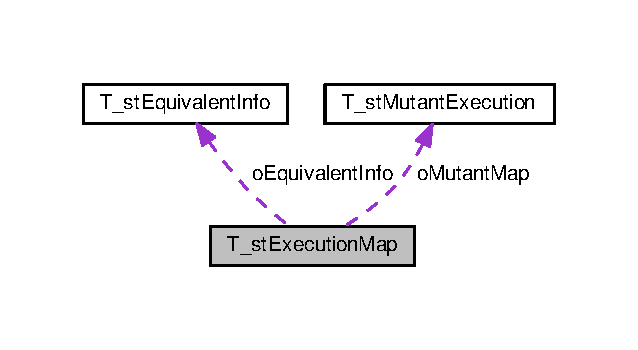
\includegraphics[width=306pt]{structT__stExecutionMap__coll__graph}
\end{center}
\end{figure}
\subsection*{Data Fields}
\begin{DoxyCompactItemize}
\item 
int \hyperlink{structT__stExecutionMap_ab3356d6f168b030b633e5f25b9a71c28}{n\-Remaining\-Mutants}
\item 
int \hyperlink{structT__stExecutionMap_afa41c6e3578ea7ae351af7b58bd3d023}{n\-Collapsed}
\item 
int \hyperlink{structT__stExecutionMap_ae8e8094bfc7fe1e6952e16866a4ff956}{n\-Index\-Mutant}
\item 
int \hyperlink{structT__stExecutionMap_a881728b28a23929150041bc561994fa6}{n\-Mutants}
\item 
int \hyperlink{structT__stExecutionMap_a8c17b23903f912f51cab70648be4fc75}{n\-Tests}
\item 
int \hyperlink{structT__stExecutionMap_aa165d4228ce93b41cd201d9482aea311}{n\-Equivalents}
\item 
int \hyperlink{structT__stExecutionMap_ad3708a1dc3093d95be783675db030a18}{n\-Dupped}
\item 
char $\ast$ \hyperlink{structT__stExecutionMap_a089e259cc95ab51ae1c134e389e739fb}{o\-Md5\-Map} \mbox{[}\hyperlink{Options_8h_a7b5fa9fc08e6e43e329c804ac562bd00}{M\-A\-X\-\_\-\-M\-U\-T\-A\-N\-T\-S}\mbox{]}
\item 
\hyperlink{structT__stEquivalentInfo}{T\-\_\-st\-Equivalent\-Info} $\ast$ \hyperlink{structT__stExecutionMap_a41d817d987562c2b69eb386534ceccce}{o\-Equivalent\-Info} \mbox{[}\hyperlink{Options_8h_a7b5fa9fc08e6e43e329c804ac562bd00}{M\-A\-X\-\_\-\-M\-U\-T\-A\-N\-T\-S}\mbox{]}
\item 
\hyperlink{structT__stMutantExecution}{T\-\_\-st\-Mutant\-Execution} $\ast$ \hyperlink{structT__stExecutionMap_a7f19bba04bd09de7b2af211dedce7dfd}{o\-Mutant\-Map} \mbox{[}\hyperlink{Options_8h_a7b5fa9fc08e6e43e329c804ac562bd00}{M\-A\-X\-\_\-\-M\-U\-T\-A\-N\-T\-S}\mbox{]}
\item 
int \hyperlink{structT__stExecutionMap_ab2e74b8fc17a93c7956c42b6155d64b1}{o\-Map} \mbox{[}\hyperlink{Options_8h_a7b5fa9fc08e6e43e329c804ac562bd00}{M\-A\-X\-\_\-\-M\-U\-T\-A\-N\-T\-S}\mbox{]}\mbox{[}\hyperlink{Options_8h_a2a77d2f2c5b698c69c19e1f8782bf709}{M\-A\-X\-\_\-\-T\-E\-S\-T\-S}\mbox{]}
\end{DoxyCompactItemize}


\subsection{Field Documentation}
\hypertarget{structT__stExecutionMap_afa41c6e3578ea7ae351af7b58bd3d023}{\index{T\-\_\-st\-Execution\-Map@{T\-\_\-st\-Execution\-Map}!n\-Collapsed@{n\-Collapsed}}
\index{n\-Collapsed@{n\-Collapsed}!T_stExecutionMap@{T\-\_\-st\-Execution\-Map}}
\subsubsection[{n\-Collapsed}]{\setlength{\rightskip}{0pt plus 5cm}int T\-\_\-st\-Execution\-Map\-::n\-Collapsed}}\label{structT__stExecutionMap_afa41c6e3578ea7ae351af7b58bd3d023}
\hypertarget{structT__stExecutionMap_ad3708a1dc3093d95be783675db030a18}{\index{T\-\_\-st\-Execution\-Map@{T\-\_\-st\-Execution\-Map}!n\-Dupped@{n\-Dupped}}
\index{n\-Dupped@{n\-Dupped}!T_stExecutionMap@{T\-\_\-st\-Execution\-Map}}
\subsubsection[{n\-Dupped}]{\setlength{\rightskip}{0pt plus 5cm}int T\-\_\-st\-Execution\-Map\-::n\-Dupped}}\label{structT__stExecutionMap_ad3708a1dc3093d95be783675db030a18}
\hypertarget{structT__stExecutionMap_aa165d4228ce93b41cd201d9482aea311}{\index{T\-\_\-st\-Execution\-Map@{T\-\_\-st\-Execution\-Map}!n\-Equivalents@{n\-Equivalents}}
\index{n\-Equivalents@{n\-Equivalents}!T_stExecutionMap@{T\-\_\-st\-Execution\-Map}}
\subsubsection[{n\-Equivalents}]{\setlength{\rightskip}{0pt plus 5cm}int T\-\_\-st\-Execution\-Map\-::n\-Equivalents}}\label{structT__stExecutionMap_aa165d4228ce93b41cd201d9482aea311}
\hypertarget{structT__stExecutionMap_ae8e8094bfc7fe1e6952e16866a4ff956}{\index{T\-\_\-st\-Execution\-Map@{T\-\_\-st\-Execution\-Map}!n\-Index\-Mutant@{n\-Index\-Mutant}}
\index{n\-Index\-Mutant@{n\-Index\-Mutant}!T_stExecutionMap@{T\-\_\-st\-Execution\-Map}}
\subsubsection[{n\-Index\-Mutant}]{\setlength{\rightskip}{0pt plus 5cm}int T\-\_\-st\-Execution\-Map\-::n\-Index\-Mutant}}\label{structT__stExecutionMap_ae8e8094bfc7fe1e6952e16866a4ff956}
\hypertarget{structT__stExecutionMap_a881728b28a23929150041bc561994fa6}{\index{T\-\_\-st\-Execution\-Map@{T\-\_\-st\-Execution\-Map}!n\-Mutants@{n\-Mutants}}
\index{n\-Mutants@{n\-Mutants}!T_stExecutionMap@{T\-\_\-st\-Execution\-Map}}
\subsubsection[{n\-Mutants}]{\setlength{\rightskip}{0pt plus 5cm}int T\-\_\-st\-Execution\-Map\-::n\-Mutants}}\label{structT__stExecutionMap_a881728b28a23929150041bc561994fa6}
\hypertarget{structT__stExecutionMap_ab3356d6f168b030b633e5f25b9a71c28}{\index{T\-\_\-st\-Execution\-Map@{T\-\_\-st\-Execution\-Map}!n\-Remaining\-Mutants@{n\-Remaining\-Mutants}}
\index{n\-Remaining\-Mutants@{n\-Remaining\-Mutants}!T_stExecutionMap@{T\-\_\-st\-Execution\-Map}}
\subsubsection[{n\-Remaining\-Mutants}]{\setlength{\rightskip}{0pt plus 5cm}int T\-\_\-st\-Execution\-Map\-::n\-Remaining\-Mutants}}\label{structT__stExecutionMap_ab3356d6f168b030b633e5f25b9a71c28}
\hypertarget{structT__stExecutionMap_a8c17b23903f912f51cab70648be4fc75}{\index{T\-\_\-st\-Execution\-Map@{T\-\_\-st\-Execution\-Map}!n\-Tests@{n\-Tests}}
\index{n\-Tests@{n\-Tests}!T_stExecutionMap@{T\-\_\-st\-Execution\-Map}}
\subsubsection[{n\-Tests}]{\setlength{\rightskip}{0pt plus 5cm}int T\-\_\-st\-Execution\-Map\-::n\-Tests}}\label{structT__stExecutionMap_a8c17b23903f912f51cab70648be4fc75}
\hypertarget{structT__stExecutionMap_a41d817d987562c2b69eb386534ceccce}{\index{T\-\_\-st\-Execution\-Map@{T\-\_\-st\-Execution\-Map}!o\-Equivalent\-Info@{o\-Equivalent\-Info}}
\index{o\-Equivalent\-Info@{o\-Equivalent\-Info}!T_stExecutionMap@{T\-\_\-st\-Execution\-Map}}
\subsubsection[{o\-Equivalent\-Info}]{\setlength{\rightskip}{0pt plus 5cm}{\bf T\-\_\-st\-Equivalent\-Info}$\ast$ T\-\_\-st\-Execution\-Map\-::o\-Equivalent\-Info\mbox{[}{\bf M\-A\-X\-\_\-\-M\-U\-T\-A\-N\-T\-S}\mbox{]}}}\label{structT__stExecutionMap_a41d817d987562c2b69eb386534ceccce}
\hypertarget{structT__stExecutionMap_ab2e74b8fc17a93c7956c42b6155d64b1}{\index{T\-\_\-st\-Execution\-Map@{T\-\_\-st\-Execution\-Map}!o\-Map@{o\-Map}}
\index{o\-Map@{o\-Map}!T_stExecutionMap@{T\-\_\-st\-Execution\-Map}}
\subsubsection[{o\-Map}]{\setlength{\rightskip}{0pt plus 5cm}int T\-\_\-st\-Execution\-Map\-::o\-Map\mbox{[}{\bf M\-A\-X\-\_\-\-M\-U\-T\-A\-N\-T\-S}\mbox{]}\mbox{[}{\bf M\-A\-X\-\_\-\-T\-E\-S\-T\-S}\mbox{]}}}\label{structT__stExecutionMap_ab2e74b8fc17a93c7956c42b6155d64b1}
\hypertarget{structT__stExecutionMap_a089e259cc95ab51ae1c134e389e739fb}{\index{T\-\_\-st\-Execution\-Map@{T\-\_\-st\-Execution\-Map}!o\-Md5\-Map@{o\-Md5\-Map}}
\index{o\-Md5\-Map@{o\-Md5\-Map}!T_stExecutionMap@{T\-\_\-st\-Execution\-Map}}
\subsubsection[{o\-Md5\-Map}]{\setlength{\rightskip}{0pt plus 5cm}char$\ast$ T\-\_\-st\-Execution\-Map\-::o\-Md5\-Map\mbox{[}{\bf M\-A\-X\-\_\-\-M\-U\-T\-A\-N\-T\-S}\mbox{]}}}\label{structT__stExecutionMap_a089e259cc95ab51ae1c134e389e739fb}
\hypertarget{structT__stExecutionMap_a7f19bba04bd09de7b2af211dedce7dfd}{\index{T\-\_\-st\-Execution\-Map@{T\-\_\-st\-Execution\-Map}!o\-Mutant\-Map@{o\-Mutant\-Map}}
\index{o\-Mutant\-Map@{o\-Mutant\-Map}!T_stExecutionMap@{T\-\_\-st\-Execution\-Map}}
\subsubsection[{o\-Mutant\-Map}]{\setlength{\rightskip}{0pt plus 5cm}{\bf T\-\_\-st\-Mutant\-Execution}$\ast$ T\-\_\-st\-Execution\-Map\-::o\-Mutant\-Map\mbox{[}{\bf M\-A\-X\-\_\-\-M\-U\-T\-A\-N\-T\-S}\mbox{]}}}\label{structT__stExecutionMap_a7f19bba04bd09de7b2af211dedce7dfd}


The documentation for this struct was generated from the following file\-:\begin{DoxyCompactItemize}
\item 
\hyperlink{Options_8h}{Options.\-h}\end{DoxyCompactItemize}

\hypertarget{structT__stExecutionStructure}{\section{T\-\_\-st\-Execution\-Structure Struct Reference}
\label{structT__stExecutionStructure}\index{T\-\_\-st\-Execution\-Structure@{T\-\_\-st\-Execution\-Structure}}
}


{\ttfamily \#include $<$Options.\-h$>$}

\subsection*{Data Fields}
\begin{DoxyCompactItemize}
\item 
int \hyperlink{structT__stExecutionStructure_aef62b95163de1f8dccbcc472c5687b90}{n\-Execution\-Mode}
\item 
int \hyperlink{structT__stExecutionStructure_aba815b781854b96b556e84b8bb358416}{n\-Mutant\-Init}
\item 
int \hyperlink{structT__stExecutionStructure_ac8fa3f0a4ca72cbd1882426f33574d5c}{n\-Mutant\-End}
\item 
int \hyperlink{structT__stExecutionStructure_adf3335889b33fa5d5137b5f0b1d2dce2}{n\-Test\-Init}
\item 
int \hyperlink{structT__stExecutionStructure_a36d89b987dd32ba06e929a5c4864c669}{n\-Test\-End}
\item 
int \hyperlink{structT__stExecutionStructure_aba070c3809e1154cba64086680fd19d9}{n\-Worker}
\item 
double \hyperlink{structT__stExecutionStructure_ac9ceb6b2fe0fb765aa705b36c2f1faf4}{d\-Init\-Tick}
\item 
double \hyperlink{structT__stExecutionStructure_a27f42d7873e49f8ae89d6c63969ef10f}{d\-End\-Tick}
\end{DoxyCompactItemize}


\subsection{Field Documentation}
\hypertarget{structT__stExecutionStructure_a27f42d7873e49f8ae89d6c63969ef10f}{\index{T\-\_\-st\-Execution\-Structure@{T\-\_\-st\-Execution\-Structure}!d\-End\-Tick@{d\-End\-Tick}}
\index{d\-End\-Tick@{d\-End\-Tick}!T_stExecutionStructure@{T\-\_\-st\-Execution\-Structure}}
\subsubsection[{d\-End\-Tick}]{\setlength{\rightskip}{0pt plus 5cm}double T\-\_\-st\-Execution\-Structure\-::d\-End\-Tick}}\label{structT__stExecutionStructure_a27f42d7873e49f8ae89d6c63969ef10f}
\hypertarget{structT__stExecutionStructure_ac9ceb6b2fe0fb765aa705b36c2f1faf4}{\index{T\-\_\-st\-Execution\-Structure@{T\-\_\-st\-Execution\-Structure}!d\-Init\-Tick@{d\-Init\-Tick}}
\index{d\-Init\-Tick@{d\-Init\-Tick}!T_stExecutionStructure@{T\-\_\-st\-Execution\-Structure}}
\subsubsection[{d\-Init\-Tick}]{\setlength{\rightskip}{0pt plus 5cm}double T\-\_\-st\-Execution\-Structure\-::d\-Init\-Tick}}\label{structT__stExecutionStructure_ac9ceb6b2fe0fb765aa705b36c2f1faf4}
\hypertarget{structT__stExecutionStructure_aef62b95163de1f8dccbcc472c5687b90}{\index{T\-\_\-st\-Execution\-Structure@{T\-\_\-st\-Execution\-Structure}!n\-Execution\-Mode@{n\-Execution\-Mode}}
\index{n\-Execution\-Mode@{n\-Execution\-Mode}!T_stExecutionStructure@{T\-\_\-st\-Execution\-Structure}}
\subsubsection[{n\-Execution\-Mode}]{\setlength{\rightskip}{0pt plus 5cm}int T\-\_\-st\-Execution\-Structure\-::n\-Execution\-Mode}}\label{structT__stExecutionStructure_aef62b95163de1f8dccbcc472c5687b90}
\hypertarget{structT__stExecutionStructure_ac8fa3f0a4ca72cbd1882426f33574d5c}{\index{T\-\_\-st\-Execution\-Structure@{T\-\_\-st\-Execution\-Structure}!n\-Mutant\-End@{n\-Mutant\-End}}
\index{n\-Mutant\-End@{n\-Mutant\-End}!T_stExecutionStructure@{T\-\_\-st\-Execution\-Structure}}
\subsubsection[{n\-Mutant\-End}]{\setlength{\rightskip}{0pt plus 5cm}int T\-\_\-st\-Execution\-Structure\-::n\-Mutant\-End}}\label{structT__stExecutionStructure_ac8fa3f0a4ca72cbd1882426f33574d5c}
\hypertarget{structT__stExecutionStructure_aba815b781854b96b556e84b8bb358416}{\index{T\-\_\-st\-Execution\-Structure@{T\-\_\-st\-Execution\-Structure}!n\-Mutant\-Init@{n\-Mutant\-Init}}
\index{n\-Mutant\-Init@{n\-Mutant\-Init}!T_stExecutionStructure@{T\-\_\-st\-Execution\-Structure}}
\subsubsection[{n\-Mutant\-Init}]{\setlength{\rightskip}{0pt plus 5cm}int T\-\_\-st\-Execution\-Structure\-::n\-Mutant\-Init}}\label{structT__stExecutionStructure_aba815b781854b96b556e84b8bb358416}
\hypertarget{structT__stExecutionStructure_a36d89b987dd32ba06e929a5c4864c669}{\index{T\-\_\-st\-Execution\-Structure@{T\-\_\-st\-Execution\-Structure}!n\-Test\-End@{n\-Test\-End}}
\index{n\-Test\-End@{n\-Test\-End}!T_stExecutionStructure@{T\-\_\-st\-Execution\-Structure}}
\subsubsection[{n\-Test\-End}]{\setlength{\rightskip}{0pt plus 5cm}int T\-\_\-st\-Execution\-Structure\-::n\-Test\-End}}\label{structT__stExecutionStructure_a36d89b987dd32ba06e929a5c4864c669}
\hypertarget{structT__stExecutionStructure_adf3335889b33fa5d5137b5f0b1d2dce2}{\index{T\-\_\-st\-Execution\-Structure@{T\-\_\-st\-Execution\-Structure}!n\-Test\-Init@{n\-Test\-Init}}
\index{n\-Test\-Init@{n\-Test\-Init}!T_stExecutionStructure@{T\-\_\-st\-Execution\-Structure}}
\subsubsection[{n\-Test\-Init}]{\setlength{\rightskip}{0pt plus 5cm}int T\-\_\-st\-Execution\-Structure\-::n\-Test\-Init}}\label{structT__stExecutionStructure_adf3335889b33fa5d5137b5f0b1d2dce2}
\hypertarget{structT__stExecutionStructure_aba070c3809e1154cba64086680fd19d9}{\index{T\-\_\-st\-Execution\-Structure@{T\-\_\-st\-Execution\-Structure}!n\-Worker@{n\-Worker}}
\index{n\-Worker@{n\-Worker}!T_stExecutionStructure@{T\-\_\-st\-Execution\-Structure}}
\subsubsection[{n\-Worker}]{\setlength{\rightskip}{0pt plus 5cm}int T\-\_\-st\-Execution\-Structure\-::n\-Worker}}\label{structT__stExecutionStructure_aba070c3809e1154cba64086680fd19d9}


The documentation for this struct was generated from the following file\-:\begin{DoxyCompactItemize}
\item 
\hyperlink{Options_8h}{Options.\-h}\end{DoxyCompactItemize}

\hypertarget{structT__stIniValues}{\section{T\-\_\-st\-Ini\-Values Struct Reference}
\label{structT__stIniValues}\index{T\-\_\-st\-Ini\-Values@{T\-\_\-st\-Ini\-Values}}
}


{\ttfamily \#include $<$configuration.\-h$>$}

\subsection*{Data Fields}
\begin{DoxyCompactItemize}
\item 
char $\ast$ \hyperlink{structT__stIniValues_ab3df825d4e72352403ee7a26433b9072}{str\-Framework}
\item 
char $\ast$ \hyperlink{structT__stIniValues_a96a9cb7f742e9dfb5d31b02365402ef8}{str\-App\-Path}
\item 
char $\ast$ \hyperlink{structT__stIniValues_ac22b85753c96ab5c7e42e276efd510ee}{str\-Mutants\-Path}
\item 
char $\ast$ \hyperlink{structT__stIniValues_a9449590564856539b23091c85e2473a2}{str\-App\-Name}
\item 
char $\ast$ \hyperlink{structT__stIniValues_a46fe9be8dc44b4ffd060a29541166e1c}{str\-Exec\-Line\-Original}
\item 
char $\ast$ \hyperlink{structT__stIniValues_a66c6ac753e7e43108c54653c43c1ab12}{str\-Exec\-Line\-Mutants}
\item 
char $\ast$ \hyperlink{structT__stIniValues_ac1f3e27f18bc3890f76a6603be93d8e5}{str\-Generation\-Mutants\-Line}
\item 
int \hyperlink{structT__stIniValues_ab4cbe3e8751c52a603337080de3fa499}{n\-Total\-Tests}
\item 
int \hyperlink{structT__stIniValues_a975e65fb143fd57b64c41e47a0b78363}{n\-Total\-Mutants}
\item 
int \hyperlink{structT__stIniValues_a7a986b1504100a3dd36231b94bca6fdc}{n\-Starting\-Mutant}
\item 
int \hyperlink{structT__stIniValues_ad4903a48760ca466c9f07d052670f80b}{n\-Distribute\-Original}
\item 
int \hyperlink{structT__stIniValues_a582f96b76a1c3f8f3bda40fb20902121}{n\-Sort\-Test\-Suite}
\item 
int \hyperlink{structT__stIniValues_a2dbfae0f34b401a1694e985f5d77bc1d}{n\-Scatter\-Workload}
\item 
int \hyperlink{structT__stIniValues_a0894f6830a07c5a2abef86eba6d21ad4}{n\-Cluster\-Mutants}
\item 
int \hyperlink{structT__stIniValues_a99916a5b870f3013258fb4d94dd267ee}{n\-Parallel\-Compilation}
\item 
int \hyperlink{structT__stIniValues_a3a381877bb58f342dde196a92a758dbe}{n\-Multiple\-Coordinators}
\item 
int \hyperlink{structT__stIniValues_a1da1d562517d22f3222f4e7ee6d5e796}{n\-Standalone}
\item 
char $\ast$ \hyperlink{structT__stIniValues_a3effe0bd84fa5aeee8f4c3f692aa8bfd}{str\-Test\-Suite\-File}
\item 
int \hyperlink{structT__stIniValues_aa1eaa1b7d87ff2a0f2ec8caec8031c60}{n\-Compilation\-Enabled}
\item 
int \hyperlink{structT__stIniValues_a146c389d29426313ef81da2437b1d3d0}{n\-Compilation\-With\-Script}
\item 
int \hyperlink{structT__stIniValues_a444ac168ec41e6247a3b067d072b1d14}{n\-Compilation\-Num\-Workers}
\item 
char $\ast$ \hyperlink{structT__stIniValues_a36dc23b7fe03594fd63814845a4e1a7f}{str\-Comp\-Script}
\item 
char $\ast$ \hyperlink{structT__stIniValues_aa0a14b65aed12b004b3573400c9dca6c}{str\-Comp\-Line\-Original}
\item 
char $\ast$ \hyperlink{structT__stIniValues_af9f6e7aaa953f711b273f3db16b3b890}{str\-Comp\-Line\-Mutants}
\item 
int \hyperlink{structT__stIniValues_a2e36a8f8b5ef4a0fb44e500769b557ee}{n\-Debug\-Max\-Original\-Timeout}
\item 
int \hyperlink{structT__stIniValues_add6f1a10197d4eac1fff112415132dae}{n\-Debug\-Max\-Mutants\-Timeout}
\item 
int \hyperlink{structT__stIniValues_a49c0c8b9a860bd7c184b048151fcab92}{n\-Debug\-Mutants\-Minimum\-Timeout}
\item 
char $\ast$ \hyperlink{structT__stIniValues_ac65031fbdca94a97851ea1d067dc5f13}{str\-Marker\-Token}
\item 
int \hyperlink{structT__stIniValues_ad8464f5bd317d855026690e7145cc15a}{n\-Mutant\-Generation\-Enabled}
\item 
int \hyperlink{structT__stIniValues_a45462c428e0bb03d4de87064d2ce6b95}{n\-Redirect\-To\-Disk\-Enabled}
\end{DoxyCompactItemize}


\subsection{Field Documentation}
\hypertarget{structT__stIniValues_a0894f6830a07c5a2abef86eba6d21ad4}{\index{T\-\_\-st\-Ini\-Values@{T\-\_\-st\-Ini\-Values}!n\-Cluster\-Mutants@{n\-Cluster\-Mutants}}
\index{n\-Cluster\-Mutants@{n\-Cluster\-Mutants}!T_stIniValues@{T\-\_\-st\-Ini\-Values}}
\subsubsection[{n\-Cluster\-Mutants}]{\setlength{\rightskip}{0pt plus 5cm}int T\-\_\-st\-Ini\-Values\-::n\-Cluster\-Mutants}}\label{structT__stIniValues_a0894f6830a07c5a2abef86eba6d21ad4}
\hypertarget{structT__stIniValues_aa1eaa1b7d87ff2a0f2ec8caec8031c60}{\index{T\-\_\-st\-Ini\-Values@{T\-\_\-st\-Ini\-Values}!n\-Compilation\-Enabled@{n\-Compilation\-Enabled}}
\index{n\-Compilation\-Enabled@{n\-Compilation\-Enabled}!T_stIniValues@{T\-\_\-st\-Ini\-Values}}
\subsubsection[{n\-Compilation\-Enabled}]{\setlength{\rightskip}{0pt plus 5cm}int T\-\_\-st\-Ini\-Values\-::n\-Compilation\-Enabled}}\label{structT__stIniValues_aa1eaa1b7d87ff2a0f2ec8caec8031c60}
\hypertarget{structT__stIniValues_a444ac168ec41e6247a3b067d072b1d14}{\index{T\-\_\-st\-Ini\-Values@{T\-\_\-st\-Ini\-Values}!n\-Compilation\-Num\-Workers@{n\-Compilation\-Num\-Workers}}
\index{n\-Compilation\-Num\-Workers@{n\-Compilation\-Num\-Workers}!T_stIniValues@{T\-\_\-st\-Ini\-Values}}
\subsubsection[{n\-Compilation\-Num\-Workers}]{\setlength{\rightskip}{0pt plus 5cm}int T\-\_\-st\-Ini\-Values\-::n\-Compilation\-Num\-Workers}}\label{structT__stIniValues_a444ac168ec41e6247a3b067d072b1d14}
\hypertarget{structT__stIniValues_a146c389d29426313ef81da2437b1d3d0}{\index{T\-\_\-st\-Ini\-Values@{T\-\_\-st\-Ini\-Values}!n\-Compilation\-With\-Script@{n\-Compilation\-With\-Script}}
\index{n\-Compilation\-With\-Script@{n\-Compilation\-With\-Script}!T_stIniValues@{T\-\_\-st\-Ini\-Values}}
\subsubsection[{n\-Compilation\-With\-Script}]{\setlength{\rightskip}{0pt plus 5cm}int T\-\_\-st\-Ini\-Values\-::n\-Compilation\-With\-Script}}\label{structT__stIniValues_a146c389d29426313ef81da2437b1d3d0}
\hypertarget{structT__stIniValues_add6f1a10197d4eac1fff112415132dae}{\index{T\-\_\-st\-Ini\-Values@{T\-\_\-st\-Ini\-Values}!n\-Debug\-Max\-Mutants\-Timeout@{n\-Debug\-Max\-Mutants\-Timeout}}
\index{n\-Debug\-Max\-Mutants\-Timeout@{n\-Debug\-Max\-Mutants\-Timeout}!T_stIniValues@{T\-\_\-st\-Ini\-Values}}
\subsubsection[{n\-Debug\-Max\-Mutants\-Timeout}]{\setlength{\rightskip}{0pt plus 5cm}int T\-\_\-st\-Ini\-Values\-::n\-Debug\-Max\-Mutants\-Timeout}}\label{structT__stIniValues_add6f1a10197d4eac1fff112415132dae}
\hypertarget{structT__stIniValues_a2e36a8f8b5ef4a0fb44e500769b557ee}{\index{T\-\_\-st\-Ini\-Values@{T\-\_\-st\-Ini\-Values}!n\-Debug\-Max\-Original\-Timeout@{n\-Debug\-Max\-Original\-Timeout}}
\index{n\-Debug\-Max\-Original\-Timeout@{n\-Debug\-Max\-Original\-Timeout}!T_stIniValues@{T\-\_\-st\-Ini\-Values}}
\subsubsection[{n\-Debug\-Max\-Original\-Timeout}]{\setlength{\rightskip}{0pt plus 5cm}int T\-\_\-st\-Ini\-Values\-::n\-Debug\-Max\-Original\-Timeout}}\label{structT__stIniValues_a2e36a8f8b5ef4a0fb44e500769b557ee}
\hypertarget{structT__stIniValues_a49c0c8b9a860bd7c184b048151fcab92}{\index{T\-\_\-st\-Ini\-Values@{T\-\_\-st\-Ini\-Values}!n\-Debug\-Mutants\-Minimum\-Timeout@{n\-Debug\-Mutants\-Minimum\-Timeout}}
\index{n\-Debug\-Mutants\-Minimum\-Timeout@{n\-Debug\-Mutants\-Minimum\-Timeout}!T_stIniValues@{T\-\_\-st\-Ini\-Values}}
\subsubsection[{n\-Debug\-Mutants\-Minimum\-Timeout}]{\setlength{\rightskip}{0pt plus 5cm}int T\-\_\-st\-Ini\-Values\-::n\-Debug\-Mutants\-Minimum\-Timeout}}\label{structT__stIniValues_a49c0c8b9a860bd7c184b048151fcab92}
\hypertarget{structT__stIniValues_ad4903a48760ca466c9f07d052670f80b}{\index{T\-\_\-st\-Ini\-Values@{T\-\_\-st\-Ini\-Values}!n\-Distribute\-Original@{n\-Distribute\-Original}}
\index{n\-Distribute\-Original@{n\-Distribute\-Original}!T_stIniValues@{T\-\_\-st\-Ini\-Values}}
\subsubsection[{n\-Distribute\-Original}]{\setlength{\rightskip}{0pt plus 5cm}int T\-\_\-st\-Ini\-Values\-::n\-Distribute\-Original}}\label{structT__stIniValues_ad4903a48760ca466c9f07d052670f80b}
\hypertarget{structT__stIniValues_a3a381877bb58f342dde196a92a758dbe}{\index{T\-\_\-st\-Ini\-Values@{T\-\_\-st\-Ini\-Values}!n\-Multiple\-Coordinators@{n\-Multiple\-Coordinators}}
\index{n\-Multiple\-Coordinators@{n\-Multiple\-Coordinators}!T_stIniValues@{T\-\_\-st\-Ini\-Values}}
\subsubsection[{n\-Multiple\-Coordinators}]{\setlength{\rightskip}{0pt plus 5cm}int T\-\_\-st\-Ini\-Values\-::n\-Multiple\-Coordinators}}\label{structT__stIniValues_a3a381877bb58f342dde196a92a758dbe}
\hypertarget{structT__stIniValues_ad8464f5bd317d855026690e7145cc15a}{\index{T\-\_\-st\-Ini\-Values@{T\-\_\-st\-Ini\-Values}!n\-Mutant\-Generation\-Enabled@{n\-Mutant\-Generation\-Enabled}}
\index{n\-Mutant\-Generation\-Enabled@{n\-Mutant\-Generation\-Enabled}!T_stIniValues@{T\-\_\-st\-Ini\-Values}}
\subsubsection[{n\-Mutant\-Generation\-Enabled}]{\setlength{\rightskip}{0pt plus 5cm}int T\-\_\-st\-Ini\-Values\-::n\-Mutant\-Generation\-Enabled}}\label{structT__stIniValues_ad8464f5bd317d855026690e7145cc15a}
\hypertarget{structT__stIniValues_a99916a5b870f3013258fb4d94dd267ee}{\index{T\-\_\-st\-Ini\-Values@{T\-\_\-st\-Ini\-Values}!n\-Parallel\-Compilation@{n\-Parallel\-Compilation}}
\index{n\-Parallel\-Compilation@{n\-Parallel\-Compilation}!T_stIniValues@{T\-\_\-st\-Ini\-Values}}
\subsubsection[{n\-Parallel\-Compilation}]{\setlength{\rightskip}{0pt plus 5cm}int T\-\_\-st\-Ini\-Values\-::n\-Parallel\-Compilation}}\label{structT__stIniValues_a99916a5b870f3013258fb4d94dd267ee}
\hypertarget{structT__stIniValues_a45462c428e0bb03d4de87064d2ce6b95}{\index{T\-\_\-st\-Ini\-Values@{T\-\_\-st\-Ini\-Values}!n\-Redirect\-To\-Disk\-Enabled@{n\-Redirect\-To\-Disk\-Enabled}}
\index{n\-Redirect\-To\-Disk\-Enabled@{n\-Redirect\-To\-Disk\-Enabled}!T_stIniValues@{T\-\_\-st\-Ini\-Values}}
\subsubsection[{n\-Redirect\-To\-Disk\-Enabled}]{\setlength{\rightskip}{0pt plus 5cm}int T\-\_\-st\-Ini\-Values\-::n\-Redirect\-To\-Disk\-Enabled}}\label{structT__stIniValues_a45462c428e0bb03d4de87064d2ce6b95}
\hypertarget{structT__stIniValues_a2dbfae0f34b401a1694e985f5d77bc1d}{\index{T\-\_\-st\-Ini\-Values@{T\-\_\-st\-Ini\-Values}!n\-Scatter\-Workload@{n\-Scatter\-Workload}}
\index{n\-Scatter\-Workload@{n\-Scatter\-Workload}!T_stIniValues@{T\-\_\-st\-Ini\-Values}}
\subsubsection[{n\-Scatter\-Workload}]{\setlength{\rightskip}{0pt plus 5cm}int T\-\_\-st\-Ini\-Values\-::n\-Scatter\-Workload}}\label{structT__stIniValues_a2dbfae0f34b401a1694e985f5d77bc1d}
\hypertarget{structT__stIniValues_a582f96b76a1c3f8f3bda40fb20902121}{\index{T\-\_\-st\-Ini\-Values@{T\-\_\-st\-Ini\-Values}!n\-Sort\-Test\-Suite@{n\-Sort\-Test\-Suite}}
\index{n\-Sort\-Test\-Suite@{n\-Sort\-Test\-Suite}!T_stIniValues@{T\-\_\-st\-Ini\-Values}}
\subsubsection[{n\-Sort\-Test\-Suite}]{\setlength{\rightskip}{0pt plus 5cm}int T\-\_\-st\-Ini\-Values\-::n\-Sort\-Test\-Suite}}\label{structT__stIniValues_a582f96b76a1c3f8f3bda40fb20902121}
\hypertarget{structT__stIniValues_a1da1d562517d22f3222f4e7ee6d5e796}{\index{T\-\_\-st\-Ini\-Values@{T\-\_\-st\-Ini\-Values}!n\-Standalone@{n\-Standalone}}
\index{n\-Standalone@{n\-Standalone}!T_stIniValues@{T\-\_\-st\-Ini\-Values}}
\subsubsection[{n\-Standalone}]{\setlength{\rightskip}{0pt plus 5cm}int T\-\_\-st\-Ini\-Values\-::n\-Standalone}}\label{structT__stIniValues_a1da1d562517d22f3222f4e7ee6d5e796}
\hypertarget{structT__stIniValues_a7a986b1504100a3dd36231b94bca6fdc}{\index{T\-\_\-st\-Ini\-Values@{T\-\_\-st\-Ini\-Values}!n\-Starting\-Mutant@{n\-Starting\-Mutant}}
\index{n\-Starting\-Mutant@{n\-Starting\-Mutant}!T_stIniValues@{T\-\_\-st\-Ini\-Values}}
\subsubsection[{n\-Starting\-Mutant}]{\setlength{\rightskip}{0pt plus 5cm}int T\-\_\-st\-Ini\-Values\-::n\-Starting\-Mutant}}\label{structT__stIniValues_a7a986b1504100a3dd36231b94bca6fdc}
\hypertarget{structT__stIniValues_a975e65fb143fd57b64c41e47a0b78363}{\index{T\-\_\-st\-Ini\-Values@{T\-\_\-st\-Ini\-Values}!n\-Total\-Mutants@{n\-Total\-Mutants}}
\index{n\-Total\-Mutants@{n\-Total\-Mutants}!T_stIniValues@{T\-\_\-st\-Ini\-Values}}
\subsubsection[{n\-Total\-Mutants}]{\setlength{\rightskip}{0pt plus 5cm}int T\-\_\-st\-Ini\-Values\-::n\-Total\-Mutants}}\label{structT__stIniValues_a975e65fb143fd57b64c41e47a0b78363}
\hypertarget{structT__stIniValues_ab4cbe3e8751c52a603337080de3fa499}{\index{T\-\_\-st\-Ini\-Values@{T\-\_\-st\-Ini\-Values}!n\-Total\-Tests@{n\-Total\-Tests}}
\index{n\-Total\-Tests@{n\-Total\-Tests}!T_stIniValues@{T\-\_\-st\-Ini\-Values}}
\subsubsection[{n\-Total\-Tests}]{\setlength{\rightskip}{0pt plus 5cm}int T\-\_\-st\-Ini\-Values\-::n\-Total\-Tests}}\label{structT__stIniValues_ab4cbe3e8751c52a603337080de3fa499}
\hypertarget{structT__stIniValues_a9449590564856539b23091c85e2473a2}{\index{T\-\_\-st\-Ini\-Values@{T\-\_\-st\-Ini\-Values}!str\-App\-Name@{str\-App\-Name}}
\index{str\-App\-Name@{str\-App\-Name}!T_stIniValues@{T\-\_\-st\-Ini\-Values}}
\subsubsection[{str\-App\-Name}]{\setlength{\rightskip}{0pt plus 5cm}char$\ast$ T\-\_\-st\-Ini\-Values\-::str\-App\-Name}}\label{structT__stIniValues_a9449590564856539b23091c85e2473a2}
\hypertarget{structT__stIniValues_a96a9cb7f742e9dfb5d31b02365402ef8}{\index{T\-\_\-st\-Ini\-Values@{T\-\_\-st\-Ini\-Values}!str\-App\-Path@{str\-App\-Path}}
\index{str\-App\-Path@{str\-App\-Path}!T_stIniValues@{T\-\_\-st\-Ini\-Values}}
\subsubsection[{str\-App\-Path}]{\setlength{\rightskip}{0pt plus 5cm}char$\ast$ T\-\_\-st\-Ini\-Values\-::str\-App\-Path}}\label{structT__stIniValues_a96a9cb7f742e9dfb5d31b02365402ef8}
\hypertarget{structT__stIniValues_af9f6e7aaa953f711b273f3db16b3b890}{\index{T\-\_\-st\-Ini\-Values@{T\-\_\-st\-Ini\-Values}!str\-Comp\-Line\-Mutants@{str\-Comp\-Line\-Mutants}}
\index{str\-Comp\-Line\-Mutants@{str\-Comp\-Line\-Mutants}!T_stIniValues@{T\-\_\-st\-Ini\-Values}}
\subsubsection[{str\-Comp\-Line\-Mutants}]{\setlength{\rightskip}{0pt plus 5cm}char$\ast$ T\-\_\-st\-Ini\-Values\-::str\-Comp\-Line\-Mutants}}\label{structT__stIniValues_af9f6e7aaa953f711b273f3db16b3b890}
\hypertarget{structT__stIniValues_aa0a14b65aed12b004b3573400c9dca6c}{\index{T\-\_\-st\-Ini\-Values@{T\-\_\-st\-Ini\-Values}!str\-Comp\-Line\-Original@{str\-Comp\-Line\-Original}}
\index{str\-Comp\-Line\-Original@{str\-Comp\-Line\-Original}!T_stIniValues@{T\-\_\-st\-Ini\-Values}}
\subsubsection[{str\-Comp\-Line\-Original}]{\setlength{\rightskip}{0pt plus 5cm}char$\ast$ T\-\_\-st\-Ini\-Values\-::str\-Comp\-Line\-Original}}\label{structT__stIniValues_aa0a14b65aed12b004b3573400c9dca6c}
\hypertarget{structT__stIniValues_a36dc23b7fe03594fd63814845a4e1a7f}{\index{T\-\_\-st\-Ini\-Values@{T\-\_\-st\-Ini\-Values}!str\-Comp\-Script@{str\-Comp\-Script}}
\index{str\-Comp\-Script@{str\-Comp\-Script}!T_stIniValues@{T\-\_\-st\-Ini\-Values}}
\subsubsection[{str\-Comp\-Script}]{\setlength{\rightskip}{0pt plus 5cm}char$\ast$ T\-\_\-st\-Ini\-Values\-::str\-Comp\-Script}}\label{structT__stIniValues_a36dc23b7fe03594fd63814845a4e1a7f}
\hypertarget{structT__stIniValues_a66c6ac753e7e43108c54653c43c1ab12}{\index{T\-\_\-st\-Ini\-Values@{T\-\_\-st\-Ini\-Values}!str\-Exec\-Line\-Mutants@{str\-Exec\-Line\-Mutants}}
\index{str\-Exec\-Line\-Mutants@{str\-Exec\-Line\-Mutants}!T_stIniValues@{T\-\_\-st\-Ini\-Values}}
\subsubsection[{str\-Exec\-Line\-Mutants}]{\setlength{\rightskip}{0pt plus 5cm}char$\ast$ T\-\_\-st\-Ini\-Values\-::str\-Exec\-Line\-Mutants}}\label{structT__stIniValues_a66c6ac753e7e43108c54653c43c1ab12}
\hypertarget{structT__stIniValues_a46fe9be8dc44b4ffd060a29541166e1c}{\index{T\-\_\-st\-Ini\-Values@{T\-\_\-st\-Ini\-Values}!str\-Exec\-Line\-Original@{str\-Exec\-Line\-Original}}
\index{str\-Exec\-Line\-Original@{str\-Exec\-Line\-Original}!T_stIniValues@{T\-\_\-st\-Ini\-Values}}
\subsubsection[{str\-Exec\-Line\-Original}]{\setlength{\rightskip}{0pt plus 5cm}char$\ast$ T\-\_\-st\-Ini\-Values\-::str\-Exec\-Line\-Original}}\label{structT__stIniValues_a46fe9be8dc44b4ffd060a29541166e1c}
\hypertarget{structT__stIniValues_ab3df825d4e72352403ee7a26433b9072}{\index{T\-\_\-st\-Ini\-Values@{T\-\_\-st\-Ini\-Values}!str\-Framework@{str\-Framework}}
\index{str\-Framework@{str\-Framework}!T_stIniValues@{T\-\_\-st\-Ini\-Values}}
\subsubsection[{str\-Framework}]{\setlength{\rightskip}{0pt plus 5cm}char$\ast$ T\-\_\-st\-Ini\-Values\-::str\-Framework}}\label{structT__stIniValues_ab3df825d4e72352403ee7a26433b9072}
\hypertarget{structT__stIniValues_ac1f3e27f18bc3890f76a6603be93d8e5}{\index{T\-\_\-st\-Ini\-Values@{T\-\_\-st\-Ini\-Values}!str\-Generation\-Mutants\-Line@{str\-Generation\-Mutants\-Line}}
\index{str\-Generation\-Mutants\-Line@{str\-Generation\-Mutants\-Line}!T_stIniValues@{T\-\_\-st\-Ini\-Values}}
\subsubsection[{str\-Generation\-Mutants\-Line}]{\setlength{\rightskip}{0pt plus 5cm}char$\ast$ T\-\_\-st\-Ini\-Values\-::str\-Generation\-Mutants\-Line}}\label{structT__stIniValues_ac1f3e27f18bc3890f76a6603be93d8e5}
\hypertarget{structT__stIniValues_ac65031fbdca94a97851ea1d067dc5f13}{\index{T\-\_\-st\-Ini\-Values@{T\-\_\-st\-Ini\-Values}!str\-Marker\-Token@{str\-Marker\-Token}}
\index{str\-Marker\-Token@{str\-Marker\-Token}!T_stIniValues@{T\-\_\-st\-Ini\-Values}}
\subsubsection[{str\-Marker\-Token}]{\setlength{\rightskip}{0pt plus 5cm}char$\ast$ T\-\_\-st\-Ini\-Values\-::str\-Marker\-Token}}\label{structT__stIniValues_ac65031fbdca94a97851ea1d067dc5f13}
\hypertarget{structT__stIniValues_ac22b85753c96ab5c7e42e276efd510ee}{\index{T\-\_\-st\-Ini\-Values@{T\-\_\-st\-Ini\-Values}!str\-Mutants\-Path@{str\-Mutants\-Path}}
\index{str\-Mutants\-Path@{str\-Mutants\-Path}!T_stIniValues@{T\-\_\-st\-Ini\-Values}}
\subsubsection[{str\-Mutants\-Path}]{\setlength{\rightskip}{0pt plus 5cm}char$\ast$ T\-\_\-st\-Ini\-Values\-::str\-Mutants\-Path}}\label{structT__stIniValues_ac22b85753c96ab5c7e42e276efd510ee}
\hypertarget{structT__stIniValues_a3effe0bd84fa5aeee8f4c3f692aa8bfd}{\index{T\-\_\-st\-Ini\-Values@{T\-\_\-st\-Ini\-Values}!str\-Test\-Suite\-File@{str\-Test\-Suite\-File}}
\index{str\-Test\-Suite\-File@{str\-Test\-Suite\-File}!T_stIniValues@{T\-\_\-st\-Ini\-Values}}
\subsubsection[{str\-Test\-Suite\-File}]{\setlength{\rightskip}{0pt plus 5cm}char$\ast$ T\-\_\-st\-Ini\-Values\-::str\-Test\-Suite\-File}}\label{structT__stIniValues_a3effe0bd84fa5aeee8f4c3f692aa8bfd}


The documentation for this struct was generated from the following file\-:\begin{DoxyCompactItemize}
\item 
\hyperlink{configuration_8h}{configuration.\-h}\end{DoxyCompactItemize}

\hypertarget{structT__stM}{\section{T\-\_\-st\-M Struct Reference}
\label{structT__stM}\index{T\-\_\-st\-M@{T\-\_\-st\-M}}
}


{\ttfamily \#include $<$Options.\-h$>$}

\subsection*{Data Fields}
\begin{DoxyCompactItemize}
\item 
int \hyperlink{structT__stM_a3e49f3f7f8adb93d6eb5121f84c33816}{n\-Number}
\item 
int \hyperlink{structT__stM_a5dd1d5b522750b22895aa1146c06c3a6}{n\-State}
\item 
int \hyperlink{structT__stM_afb940fe5fd0991972e5ee8822805d10e}{n\-Test\-Killer}
\item 
int \hyperlink{structT__stM_a145001a7ab272ff272400d654985aaed}{n\-Tests}
\item 
double \hyperlink{structT__stM_a3b6e012242e88dd2c27e90bea06c3ef5}{o\-Time} \mbox{[}\hyperlink{Options_8h_a2a77d2f2c5b698c69c19e1f8782bf709}{M\-A\-X\-\_\-\-T\-E\-S\-T\-S}\mbox{]}
\item 
int \hyperlink{structT__stM_a607d25dfebe1f4c7fa623e1c11e596ac}{o\-Kill} \mbox{[}\hyperlink{Options_8h_a2a77d2f2c5b698c69c19e1f8782bf709}{M\-A\-X\-\_\-\-T\-E\-S\-T\-S}\mbox{]}
\item 
int \hyperlink{structT__stM_a96a05b3681ffbe7e0f1a8ee95b74fa3a}{o\-Test} \mbox{[}\hyperlink{Options_8h_a2a77d2f2c5b698c69c19e1f8782bf709}{M\-A\-X\-\_\-\-T\-E\-S\-T\-S}\mbox{]}
\end{DoxyCompactItemize}


\subsection{Field Documentation}
\hypertarget{structT__stM_a3e49f3f7f8adb93d6eb5121f84c33816}{\index{T\-\_\-st\-M@{T\-\_\-st\-M}!n\-Number@{n\-Number}}
\index{n\-Number@{n\-Number}!T_stM@{T\-\_\-st\-M}}
\subsubsection[{n\-Number}]{\setlength{\rightskip}{0pt plus 5cm}int T\-\_\-st\-M\-::n\-Number}}\label{structT__stM_a3e49f3f7f8adb93d6eb5121f84c33816}
\hypertarget{structT__stM_a5dd1d5b522750b22895aa1146c06c3a6}{\index{T\-\_\-st\-M@{T\-\_\-st\-M}!n\-State@{n\-State}}
\index{n\-State@{n\-State}!T_stM@{T\-\_\-st\-M}}
\subsubsection[{n\-State}]{\setlength{\rightskip}{0pt plus 5cm}int T\-\_\-st\-M\-::n\-State}}\label{structT__stM_a5dd1d5b522750b22895aa1146c06c3a6}
\hypertarget{structT__stM_afb940fe5fd0991972e5ee8822805d10e}{\index{T\-\_\-st\-M@{T\-\_\-st\-M}!n\-Test\-Killer@{n\-Test\-Killer}}
\index{n\-Test\-Killer@{n\-Test\-Killer}!T_stM@{T\-\_\-st\-M}}
\subsubsection[{n\-Test\-Killer}]{\setlength{\rightskip}{0pt plus 5cm}int T\-\_\-st\-M\-::n\-Test\-Killer}}\label{structT__stM_afb940fe5fd0991972e5ee8822805d10e}
\hypertarget{structT__stM_a145001a7ab272ff272400d654985aaed}{\index{T\-\_\-st\-M@{T\-\_\-st\-M}!n\-Tests@{n\-Tests}}
\index{n\-Tests@{n\-Tests}!T_stM@{T\-\_\-st\-M}}
\subsubsection[{n\-Tests}]{\setlength{\rightskip}{0pt plus 5cm}int T\-\_\-st\-M\-::n\-Tests}}\label{structT__stM_a145001a7ab272ff272400d654985aaed}
\hypertarget{structT__stM_a607d25dfebe1f4c7fa623e1c11e596ac}{\index{T\-\_\-st\-M@{T\-\_\-st\-M}!o\-Kill@{o\-Kill}}
\index{o\-Kill@{o\-Kill}!T_stM@{T\-\_\-st\-M}}
\subsubsection[{o\-Kill}]{\setlength{\rightskip}{0pt plus 5cm}int T\-\_\-st\-M\-::o\-Kill\mbox{[}{\bf M\-A\-X\-\_\-\-T\-E\-S\-T\-S}\mbox{]}}}\label{structT__stM_a607d25dfebe1f4c7fa623e1c11e596ac}
\hypertarget{structT__stM_a96a05b3681ffbe7e0f1a8ee95b74fa3a}{\index{T\-\_\-st\-M@{T\-\_\-st\-M}!o\-Test@{o\-Test}}
\index{o\-Test@{o\-Test}!T_stM@{T\-\_\-st\-M}}
\subsubsection[{o\-Test}]{\setlength{\rightskip}{0pt plus 5cm}int T\-\_\-st\-M\-::o\-Test\mbox{[}{\bf M\-A\-X\-\_\-\-T\-E\-S\-T\-S}\mbox{]}}}\label{structT__stM_a96a05b3681ffbe7e0f1a8ee95b74fa3a}
\hypertarget{structT__stM_a3b6e012242e88dd2c27e90bea06c3ef5}{\index{T\-\_\-st\-M@{T\-\_\-st\-M}!o\-Time@{o\-Time}}
\index{o\-Time@{o\-Time}!T_stM@{T\-\_\-st\-M}}
\subsubsection[{o\-Time}]{\setlength{\rightskip}{0pt plus 5cm}double T\-\_\-st\-M\-::o\-Time\mbox{[}{\bf M\-A\-X\-\_\-\-T\-E\-S\-T\-S}\mbox{]}}}\label{structT__stM_a3b6e012242e88dd2c27e90bea06c3ef5}


The documentation for this struct was generated from the following file\-:\begin{DoxyCompactItemize}
\item 
\hyperlink{Options_8h}{Options.\-h}\end{DoxyCompactItemize}

\hypertarget{structT__stMutant}{\section{T\-\_\-st\-Mutant Struct Reference}
\label{structT__stMutant}\index{T\-\_\-st\-Mutant@{T\-\_\-st\-Mutant}}
}


{\ttfamily \#include $<$Options.\-h$>$}



Collaboration diagram for T\-\_\-st\-Mutant\-:\nopagebreak
\begin{figure}[H]
\begin{center}
\leavevmode
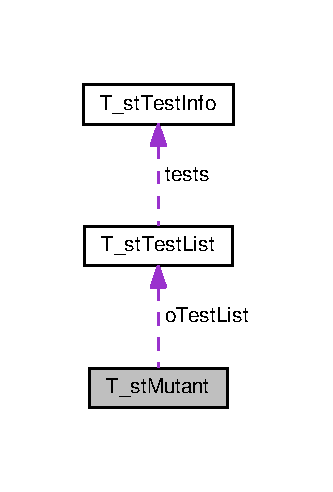
\includegraphics[width=160pt]{structT__stMutant__coll__graph}
\end{center}
\end{figure}
\subsection*{Data Fields}
\begin{DoxyCompactItemize}
\item 
int \hyperlink{structT__stMutant_aa786929cdfa4a262bb6d760443b3025d}{n\-Number}
\item 
int \hyperlink{structT__stMutant_ada5890ac8d2defb9096bc5dcef0965ee}{n\-State}
\item 
int \hyperlink{structT__stMutant_a4e9fc72bb0ca2c52d21f7622514b0106}{n\-Test\-Killer}
\item 
char $\ast$ \hyperlink{structT__stMutant_a0593f27426124cd3d47d8e032b08d56e}{str\-Description}
\item 
\hyperlink{structT__stTestList}{T\-\_\-st\-Test\-List} \hyperlink{structT__stMutant_a526593dc889002d1c2cd1ee66c9b6325}{o\-Test\-List}
\end{DoxyCompactItemize}


\subsection{Field Documentation}
\hypertarget{structT__stMutant_aa786929cdfa4a262bb6d760443b3025d}{\index{T\-\_\-st\-Mutant@{T\-\_\-st\-Mutant}!n\-Number@{n\-Number}}
\index{n\-Number@{n\-Number}!T_stMutant@{T\-\_\-st\-Mutant}}
\subsubsection[{n\-Number}]{\setlength{\rightskip}{0pt plus 5cm}int T\-\_\-st\-Mutant\-::n\-Number}}\label{structT__stMutant_aa786929cdfa4a262bb6d760443b3025d}
\hypertarget{structT__stMutant_ada5890ac8d2defb9096bc5dcef0965ee}{\index{T\-\_\-st\-Mutant@{T\-\_\-st\-Mutant}!n\-State@{n\-State}}
\index{n\-State@{n\-State}!T_stMutant@{T\-\_\-st\-Mutant}}
\subsubsection[{n\-State}]{\setlength{\rightskip}{0pt plus 5cm}int T\-\_\-st\-Mutant\-::n\-State}}\label{structT__stMutant_ada5890ac8d2defb9096bc5dcef0965ee}
\hypertarget{structT__stMutant_a4e9fc72bb0ca2c52d21f7622514b0106}{\index{T\-\_\-st\-Mutant@{T\-\_\-st\-Mutant}!n\-Test\-Killer@{n\-Test\-Killer}}
\index{n\-Test\-Killer@{n\-Test\-Killer}!T_stMutant@{T\-\_\-st\-Mutant}}
\subsubsection[{n\-Test\-Killer}]{\setlength{\rightskip}{0pt plus 5cm}int T\-\_\-st\-Mutant\-::n\-Test\-Killer}}\label{structT__stMutant_a4e9fc72bb0ca2c52d21f7622514b0106}
\hypertarget{structT__stMutant_a526593dc889002d1c2cd1ee66c9b6325}{\index{T\-\_\-st\-Mutant@{T\-\_\-st\-Mutant}!o\-Test\-List@{o\-Test\-List}}
\index{o\-Test\-List@{o\-Test\-List}!T_stMutant@{T\-\_\-st\-Mutant}}
\subsubsection[{o\-Test\-List}]{\setlength{\rightskip}{0pt plus 5cm}{\bf T\-\_\-st\-Test\-List} T\-\_\-st\-Mutant\-::o\-Test\-List}}\label{structT__stMutant_a526593dc889002d1c2cd1ee66c9b6325}
\hypertarget{structT__stMutant_a0593f27426124cd3d47d8e032b08d56e}{\index{T\-\_\-st\-Mutant@{T\-\_\-st\-Mutant}!str\-Description@{str\-Description}}
\index{str\-Description@{str\-Description}!T_stMutant@{T\-\_\-st\-Mutant}}
\subsubsection[{str\-Description}]{\setlength{\rightskip}{0pt plus 5cm}char$\ast$ T\-\_\-st\-Mutant\-::str\-Description}}\label{structT__stMutant_a0593f27426124cd3d47d8e032b08d56e}


The documentation for this struct was generated from the following file\-:\begin{DoxyCompactItemize}
\item 
\hyperlink{Options_8h}{Options.\-h}\end{DoxyCompactItemize}

\hypertarget{structT__stMutantExecution}{\section{T\-\_\-st\-Mutant\-Execution Struct Reference}
\label{structT__stMutantExecution}\index{T\-\_\-st\-Mutant\-Execution@{T\-\_\-st\-Mutant\-Execution}}
}


{\ttfamily \#include $<$Options.\-h$>$}

\subsection*{Data Fields}
\begin{DoxyCompactItemize}
\item 
int \hyperlink{structT__stMutantExecution_aad0159845c8a654cec6e68c0887be609}{n\-Equivalent}
\item 
int \hyperlink{structT__stMutantExecution_a892cc030241593320f55fbabfa060679}{n\-Is\-Clustered}
\item 
int \hyperlink{structT__stMutantExecution_a3bd80a5e3e6c5cf647a62dfb0b694bcf}{n\-Managed}
\item 
int \hyperlink{structT__stMutantExecution_a56ecf18ce5bc925a81abd45096ccc155}{n\-Finished}
\item 
int \hyperlink{structT__stMutantExecution_a8cbb62d7c67ff6a7c0e09ddd0f1e87ca}{n\-Index\-Test}
\end{DoxyCompactItemize}


\subsection{Field Documentation}
\hypertarget{structT__stMutantExecution_aad0159845c8a654cec6e68c0887be609}{\index{T\-\_\-st\-Mutant\-Execution@{T\-\_\-st\-Mutant\-Execution}!n\-Equivalent@{n\-Equivalent}}
\index{n\-Equivalent@{n\-Equivalent}!T_stMutantExecution@{T\-\_\-st\-Mutant\-Execution}}
\subsubsection[{n\-Equivalent}]{\setlength{\rightskip}{0pt plus 5cm}int T\-\_\-st\-Mutant\-Execution\-::n\-Equivalent}}\label{structT__stMutantExecution_aad0159845c8a654cec6e68c0887be609}
\hypertarget{structT__stMutantExecution_a56ecf18ce5bc925a81abd45096ccc155}{\index{T\-\_\-st\-Mutant\-Execution@{T\-\_\-st\-Mutant\-Execution}!n\-Finished@{n\-Finished}}
\index{n\-Finished@{n\-Finished}!T_stMutantExecution@{T\-\_\-st\-Mutant\-Execution}}
\subsubsection[{n\-Finished}]{\setlength{\rightskip}{0pt plus 5cm}int T\-\_\-st\-Mutant\-Execution\-::n\-Finished}}\label{structT__stMutantExecution_a56ecf18ce5bc925a81abd45096ccc155}
\hypertarget{structT__stMutantExecution_a8cbb62d7c67ff6a7c0e09ddd0f1e87ca}{\index{T\-\_\-st\-Mutant\-Execution@{T\-\_\-st\-Mutant\-Execution}!n\-Index\-Test@{n\-Index\-Test}}
\index{n\-Index\-Test@{n\-Index\-Test}!T_stMutantExecution@{T\-\_\-st\-Mutant\-Execution}}
\subsubsection[{n\-Index\-Test}]{\setlength{\rightskip}{0pt plus 5cm}int T\-\_\-st\-Mutant\-Execution\-::n\-Index\-Test}}\label{structT__stMutantExecution_a8cbb62d7c67ff6a7c0e09ddd0f1e87ca}
\hypertarget{structT__stMutantExecution_a892cc030241593320f55fbabfa060679}{\index{T\-\_\-st\-Mutant\-Execution@{T\-\_\-st\-Mutant\-Execution}!n\-Is\-Clustered@{n\-Is\-Clustered}}
\index{n\-Is\-Clustered@{n\-Is\-Clustered}!T_stMutantExecution@{T\-\_\-st\-Mutant\-Execution}}
\subsubsection[{n\-Is\-Clustered}]{\setlength{\rightskip}{0pt plus 5cm}int T\-\_\-st\-Mutant\-Execution\-::n\-Is\-Clustered}}\label{structT__stMutantExecution_a892cc030241593320f55fbabfa060679}
\hypertarget{structT__stMutantExecution_a3bd80a5e3e6c5cf647a62dfb0b694bcf}{\index{T\-\_\-st\-Mutant\-Execution@{T\-\_\-st\-Mutant\-Execution}!n\-Managed@{n\-Managed}}
\index{n\-Managed@{n\-Managed}!T_stMutantExecution@{T\-\_\-st\-Mutant\-Execution}}
\subsubsection[{n\-Managed}]{\setlength{\rightskip}{0pt plus 5cm}int T\-\_\-st\-Mutant\-Execution\-::n\-Managed}}\label{structT__stMutantExecution_a3bd80a5e3e6c5cf647a62dfb0b694bcf}


The documentation for this struct was generated from the following file\-:\begin{DoxyCompactItemize}
\item 
\hyperlink{Options_8h}{Options.\-h}\end{DoxyCompactItemize}

\hypertarget{structT__stTestInfo}{\section{T\-\_\-st\-Test\-Info Struct Reference}
\label{structT__stTestInfo}\index{T\-\_\-st\-Test\-Info@{T\-\_\-st\-Test\-Info}}
}


{\ttfamily \#include $<$Options.\-h$>$}

\subsection*{Data Fields}
\begin{DoxyCompactItemize}
\item 
char \hyperlink{structT__stTestInfo_aa38c547822e2dc65413e36b01a0c146b}{res} \mbox{[}\hyperlink{Options_8h_ae9b9a76449e4c445a7462cedf31b5805}{M\-A\-X\-\_\-\-R\-E\-S\-U\-L\-T\-\_\-\-S\-I\-Z\-E}\mbox{]}
\item 
double \hyperlink{structT__stTestInfo_a5e5ce59f759e44a4c770bc9aec9becd9}{d\-Time}
\item 
double \hyperlink{structT__stTestInfo_abab4bc2b273e308f14654bdfc92374ef}{d\-Init\-Tick}
\item 
double \hyperlink{structT__stTestInfo_ad07fd2d330a0aaaaf7b10e5fb6e09d98}{d\-End\-Tick}
\item 
int \hyperlink{structT__stTestInfo_a8252b126792e879c5b724f13e3ea7c44}{n\-Kill}
\item 
int \hyperlink{structT__stTestInfo_a31008dedf18028d566bb3f3b4732d817}{n\-Test}
\end{DoxyCompactItemize}


\subsection{Field Documentation}
\hypertarget{structT__stTestInfo_ad07fd2d330a0aaaaf7b10e5fb6e09d98}{\index{T\-\_\-st\-Test\-Info@{T\-\_\-st\-Test\-Info}!d\-End\-Tick@{d\-End\-Tick}}
\index{d\-End\-Tick@{d\-End\-Tick}!T_stTestInfo@{T\-\_\-st\-Test\-Info}}
\subsubsection[{d\-End\-Tick}]{\setlength{\rightskip}{0pt plus 5cm}double T\-\_\-st\-Test\-Info\-::d\-End\-Tick}}\label{structT__stTestInfo_ad07fd2d330a0aaaaf7b10e5fb6e09d98}
\hypertarget{structT__stTestInfo_abab4bc2b273e308f14654bdfc92374ef}{\index{T\-\_\-st\-Test\-Info@{T\-\_\-st\-Test\-Info}!d\-Init\-Tick@{d\-Init\-Tick}}
\index{d\-Init\-Tick@{d\-Init\-Tick}!T_stTestInfo@{T\-\_\-st\-Test\-Info}}
\subsubsection[{d\-Init\-Tick}]{\setlength{\rightskip}{0pt plus 5cm}double T\-\_\-st\-Test\-Info\-::d\-Init\-Tick}}\label{structT__stTestInfo_abab4bc2b273e308f14654bdfc92374ef}
\hypertarget{structT__stTestInfo_a5e5ce59f759e44a4c770bc9aec9becd9}{\index{T\-\_\-st\-Test\-Info@{T\-\_\-st\-Test\-Info}!d\-Time@{d\-Time}}
\index{d\-Time@{d\-Time}!T_stTestInfo@{T\-\_\-st\-Test\-Info}}
\subsubsection[{d\-Time}]{\setlength{\rightskip}{0pt plus 5cm}double T\-\_\-st\-Test\-Info\-::d\-Time}}\label{structT__stTestInfo_a5e5ce59f759e44a4c770bc9aec9becd9}
\hypertarget{structT__stTestInfo_a8252b126792e879c5b724f13e3ea7c44}{\index{T\-\_\-st\-Test\-Info@{T\-\_\-st\-Test\-Info}!n\-Kill@{n\-Kill}}
\index{n\-Kill@{n\-Kill}!T_stTestInfo@{T\-\_\-st\-Test\-Info}}
\subsubsection[{n\-Kill}]{\setlength{\rightskip}{0pt plus 5cm}int T\-\_\-st\-Test\-Info\-::n\-Kill}}\label{structT__stTestInfo_a8252b126792e879c5b724f13e3ea7c44}
\hypertarget{structT__stTestInfo_a31008dedf18028d566bb3f3b4732d817}{\index{T\-\_\-st\-Test\-Info@{T\-\_\-st\-Test\-Info}!n\-Test@{n\-Test}}
\index{n\-Test@{n\-Test}!T_stTestInfo@{T\-\_\-st\-Test\-Info}}
\subsubsection[{n\-Test}]{\setlength{\rightskip}{0pt plus 5cm}int T\-\_\-st\-Test\-Info\-::n\-Test}}\label{structT__stTestInfo_a31008dedf18028d566bb3f3b4732d817}
\hypertarget{structT__stTestInfo_aa38c547822e2dc65413e36b01a0c146b}{\index{T\-\_\-st\-Test\-Info@{T\-\_\-st\-Test\-Info}!res@{res}}
\index{res@{res}!T_stTestInfo@{T\-\_\-st\-Test\-Info}}
\subsubsection[{res}]{\setlength{\rightskip}{0pt plus 5cm}char T\-\_\-st\-Test\-Info\-::res\mbox{[}{\bf M\-A\-X\-\_\-\-R\-E\-S\-U\-L\-T\-\_\-\-S\-I\-Z\-E}\mbox{]}}}\label{structT__stTestInfo_aa38c547822e2dc65413e36b01a0c146b}


The documentation for this struct was generated from the following file\-:\begin{DoxyCompactItemize}
\item 
\hyperlink{Options_8h}{Options.\-h}\end{DoxyCompactItemize}

\hypertarget{structT__stTestList}{\section{T\-\_\-st\-Test\-List Struct Reference}
\label{structT__stTestList}\index{T\-\_\-st\-Test\-List@{T\-\_\-st\-Test\-List}}
}


{\ttfamily \#include $<$Options.\-h$>$}



Collaboration diagram for T\-\_\-st\-Test\-List\-:\nopagebreak
\begin{figure}[H]
\begin{center}
\leavevmode
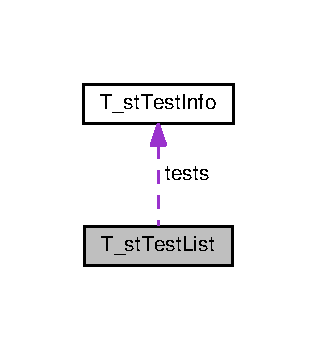
\includegraphics[width=152pt]{structT__stTestList__coll__graph}
\end{center}
\end{figure}
\subsection*{Data Fields}
\begin{DoxyCompactItemize}
\item 
int \hyperlink{structT__stTestList_a3c0aa528e2fcb76dee4bfed8cc6af283}{n\-Elems}
\item 
int \hyperlink{structT__stTestList_a957fc1ce837a0da88887b9fd92aed436}{n\-Max}
\item 
\hyperlink{structT__stTestInfo}{T\-\_\-st\-Test\-Info} $\ast$ \hyperlink{structT__stTestList_a73e25f5a90fc3e8c56dc5bdfb3a94495}{tests} \mbox{[}\hyperlink{Options_8h_a2a77d2f2c5b698c69c19e1f8782bf709}{M\-A\-X\-\_\-\-T\-E\-S\-T\-S}\mbox{]}
\end{DoxyCompactItemize}


\subsection{Field Documentation}
\hypertarget{structT__stTestList_a3c0aa528e2fcb76dee4bfed8cc6af283}{\index{T\-\_\-st\-Test\-List@{T\-\_\-st\-Test\-List}!n\-Elems@{n\-Elems}}
\index{n\-Elems@{n\-Elems}!T_stTestList@{T\-\_\-st\-Test\-List}}
\subsubsection[{n\-Elems}]{\setlength{\rightskip}{0pt plus 5cm}int T\-\_\-st\-Test\-List\-::n\-Elems}}\label{structT__stTestList_a3c0aa528e2fcb76dee4bfed8cc6af283}
\hypertarget{structT__stTestList_a957fc1ce837a0da88887b9fd92aed436}{\index{T\-\_\-st\-Test\-List@{T\-\_\-st\-Test\-List}!n\-Max@{n\-Max}}
\index{n\-Max@{n\-Max}!T_stTestList@{T\-\_\-st\-Test\-List}}
\subsubsection[{n\-Max}]{\setlength{\rightskip}{0pt plus 5cm}int T\-\_\-st\-Test\-List\-::n\-Max}}\label{structT__stTestList_a957fc1ce837a0da88887b9fd92aed436}
\hypertarget{structT__stTestList_a73e25f5a90fc3e8c56dc5bdfb3a94495}{\index{T\-\_\-st\-Test\-List@{T\-\_\-st\-Test\-List}!tests@{tests}}
\index{tests@{tests}!T_stTestList@{T\-\_\-st\-Test\-List}}
\subsubsection[{tests}]{\setlength{\rightskip}{0pt plus 5cm}{\bf T\-\_\-st\-Test\-Info}$\ast$ T\-\_\-st\-Test\-List\-::tests\mbox{[}{\bf M\-A\-X\-\_\-\-T\-E\-S\-T\-S}\mbox{]}}}\label{structT__stTestList_a73e25f5a90fc3e8c56dc5bdfb3a94495}


The documentation for this struct was generated from the following file\-:\begin{DoxyCompactItemize}
\item 
\hyperlink{Options_8h}{Options.\-h}\end{DoxyCompactItemize}

\hypertarget{structT__stTI}{\section{T\-\_\-st\-T\-I Struct Reference}
\label{structT__stTI}\index{T\-\_\-st\-T\-I@{T\-\_\-st\-T\-I}}
}


{\ttfamily \#include $<$Options.\-h$>$}

\subsection*{Data Fields}
\begin{DoxyCompactItemize}
\item 
char \hyperlink{structT__stTI_ac05a161709d3f1eec760d11aa13fc0b7}{res} \mbox{[}\hyperlink{Options_8h_ae9b9a76449e4c445a7462cedf31b5805}{M\-A\-X\-\_\-\-R\-E\-S\-U\-L\-T\-\_\-\-S\-I\-Z\-E}\mbox{]}
\item 
double \hyperlink{structT__stTI_ac66faf2192de9672574effb26319b45f}{d\-Time}
\item 
int \hyperlink{structT__stTI_ad62dfc2b1cd7514a9d587d2869972be7}{n\-Kill}
\item 
int \hyperlink{structT__stTI_a961acc1a141fcef1ccd9c5e492c5b2a9}{n\-Test}
\item 
int \hyperlink{structT__stTI_a4a30d643762e8a2c31455bc188395496}{n\-Mutant}
\end{DoxyCompactItemize}


\subsection{Field Documentation}
\hypertarget{structT__stTI_ac66faf2192de9672574effb26319b45f}{\index{T\-\_\-st\-T\-I@{T\-\_\-st\-T\-I}!d\-Time@{d\-Time}}
\index{d\-Time@{d\-Time}!T_stTI@{T\-\_\-st\-T\-I}}
\subsubsection[{d\-Time}]{\setlength{\rightskip}{0pt plus 5cm}double T\-\_\-st\-T\-I\-::d\-Time}}\label{structT__stTI_ac66faf2192de9672574effb26319b45f}
\hypertarget{structT__stTI_ad62dfc2b1cd7514a9d587d2869972be7}{\index{T\-\_\-st\-T\-I@{T\-\_\-st\-T\-I}!n\-Kill@{n\-Kill}}
\index{n\-Kill@{n\-Kill}!T_stTI@{T\-\_\-st\-T\-I}}
\subsubsection[{n\-Kill}]{\setlength{\rightskip}{0pt plus 5cm}int T\-\_\-st\-T\-I\-::n\-Kill}}\label{structT__stTI_ad62dfc2b1cd7514a9d587d2869972be7}
\hypertarget{structT__stTI_a4a30d643762e8a2c31455bc188395496}{\index{T\-\_\-st\-T\-I@{T\-\_\-st\-T\-I}!n\-Mutant@{n\-Mutant}}
\index{n\-Mutant@{n\-Mutant}!T_stTI@{T\-\_\-st\-T\-I}}
\subsubsection[{n\-Mutant}]{\setlength{\rightskip}{0pt plus 5cm}int T\-\_\-st\-T\-I\-::n\-Mutant}}\label{structT__stTI_a4a30d643762e8a2c31455bc188395496}
\hypertarget{structT__stTI_a961acc1a141fcef1ccd9c5e492c5b2a9}{\index{T\-\_\-st\-T\-I@{T\-\_\-st\-T\-I}!n\-Test@{n\-Test}}
\index{n\-Test@{n\-Test}!T_stTI@{T\-\_\-st\-T\-I}}
\subsubsection[{n\-Test}]{\setlength{\rightskip}{0pt plus 5cm}int T\-\_\-st\-T\-I\-::n\-Test}}\label{structT__stTI_a961acc1a141fcef1ccd9c5e492c5b2a9}
\hypertarget{structT__stTI_ac05a161709d3f1eec760d11aa13fc0b7}{\index{T\-\_\-st\-T\-I@{T\-\_\-st\-T\-I}!res@{res}}
\index{res@{res}!T_stTI@{T\-\_\-st\-T\-I}}
\subsubsection[{res}]{\setlength{\rightskip}{0pt plus 5cm}char T\-\_\-st\-T\-I\-::res\mbox{[}{\bf M\-A\-X\-\_\-\-R\-E\-S\-U\-L\-T\-\_\-\-S\-I\-Z\-E}\mbox{]}}}\label{structT__stTI_ac05a161709d3f1eec760d11aa13fc0b7}


The documentation for this struct was generated from the following file\-:\begin{DoxyCompactItemize}
\item 
\hyperlink{Options_8h}{Options.\-h}\end{DoxyCompactItemize}

\hypertarget{structVector}{\section{Vector Struct Reference}
\label{structVector}\index{Vector@{Vector}}
}


{\ttfamily \#include $<$Vector.\-h$>$}

\subsection*{Data Fields}
\begin{DoxyCompactItemize}
\item 
int \hyperlink{structVector_ae13c6e730a6558ba444beb8f7e44d4ca}{size}
\item 
int \hyperlink{structVector_a6d49b240ab4a8ccb9b1c7297e78511da}{capacity}
\item 
int $\ast$ \hyperlink{structVector_a67bbdb285c3d50f63e79c214cf0735a8}{data}
\end{DoxyCompactItemize}


\subsection{Field Documentation}
\hypertarget{structVector_a6d49b240ab4a8ccb9b1c7297e78511da}{\index{Vector@{Vector}!capacity@{capacity}}
\index{capacity@{capacity}!Vector@{Vector}}
\subsubsection[{capacity}]{\setlength{\rightskip}{0pt plus 5cm}int Vector\-::capacity}}\label{structVector_a6d49b240ab4a8ccb9b1c7297e78511da}
\hypertarget{structVector_a67bbdb285c3d50f63e79c214cf0735a8}{\index{Vector@{Vector}!data@{data}}
\index{data@{data}!Vector@{Vector}}
\subsubsection[{data}]{\setlength{\rightskip}{0pt plus 5cm}int$\ast$ Vector\-::data}}\label{structVector_a67bbdb285c3d50f63e79c214cf0735a8}
\hypertarget{structVector_ae13c6e730a6558ba444beb8f7e44d4ca}{\index{Vector@{Vector}!size@{size}}
\index{size@{size}!Vector@{Vector}}
\subsubsection[{size}]{\setlength{\rightskip}{0pt plus 5cm}int Vector\-::size}}\label{structVector_ae13c6e730a6558ba444beb8f7e44d4ca}


The documentation for this struct was generated from the following file\-:\begin{DoxyCompactItemize}
\item 
\hyperlink{Vector_8h}{Vector.\-h}\end{DoxyCompactItemize}

\chapter{File Documentation}
\hypertarget{_8dep_8inc}{\section{.dep.\-inc File Reference}
\label{_8dep_8inc}\index{.\-dep.\-inc@{.\-dep.\-inc}}
}

\hypertarget{Auxiliars_8c}{\section{Auxiliars.\-c File Reference}
\label{Auxiliars_8c}\index{Auxiliars.\-c@{Auxiliars.\-c}}
}
{\ttfamily \#include \char`\"{}Options.\-h\char`\"{}}\\*
{\ttfamily \#include \char`\"{}Auxiliars.\-h\char`\"{}}\\*
{\ttfamily \#include \char`\"{}Malone.\-h\char`\"{}}\\*
{\ttfamily \#include $<$errno.\-h$>$}\\*
{\ttfamily \#include $<$fcntl.\-h$>$}\\*
{\ttfamily \#include $<$unistd.\-h$>$}\\*
{\ttfamily \#include $<$sys/wait.\-h$>$}\\*
Include dependency graph for Auxiliars.\-c\-:\nopagebreak
\begin{figure}[H]
\begin{center}
\leavevmode
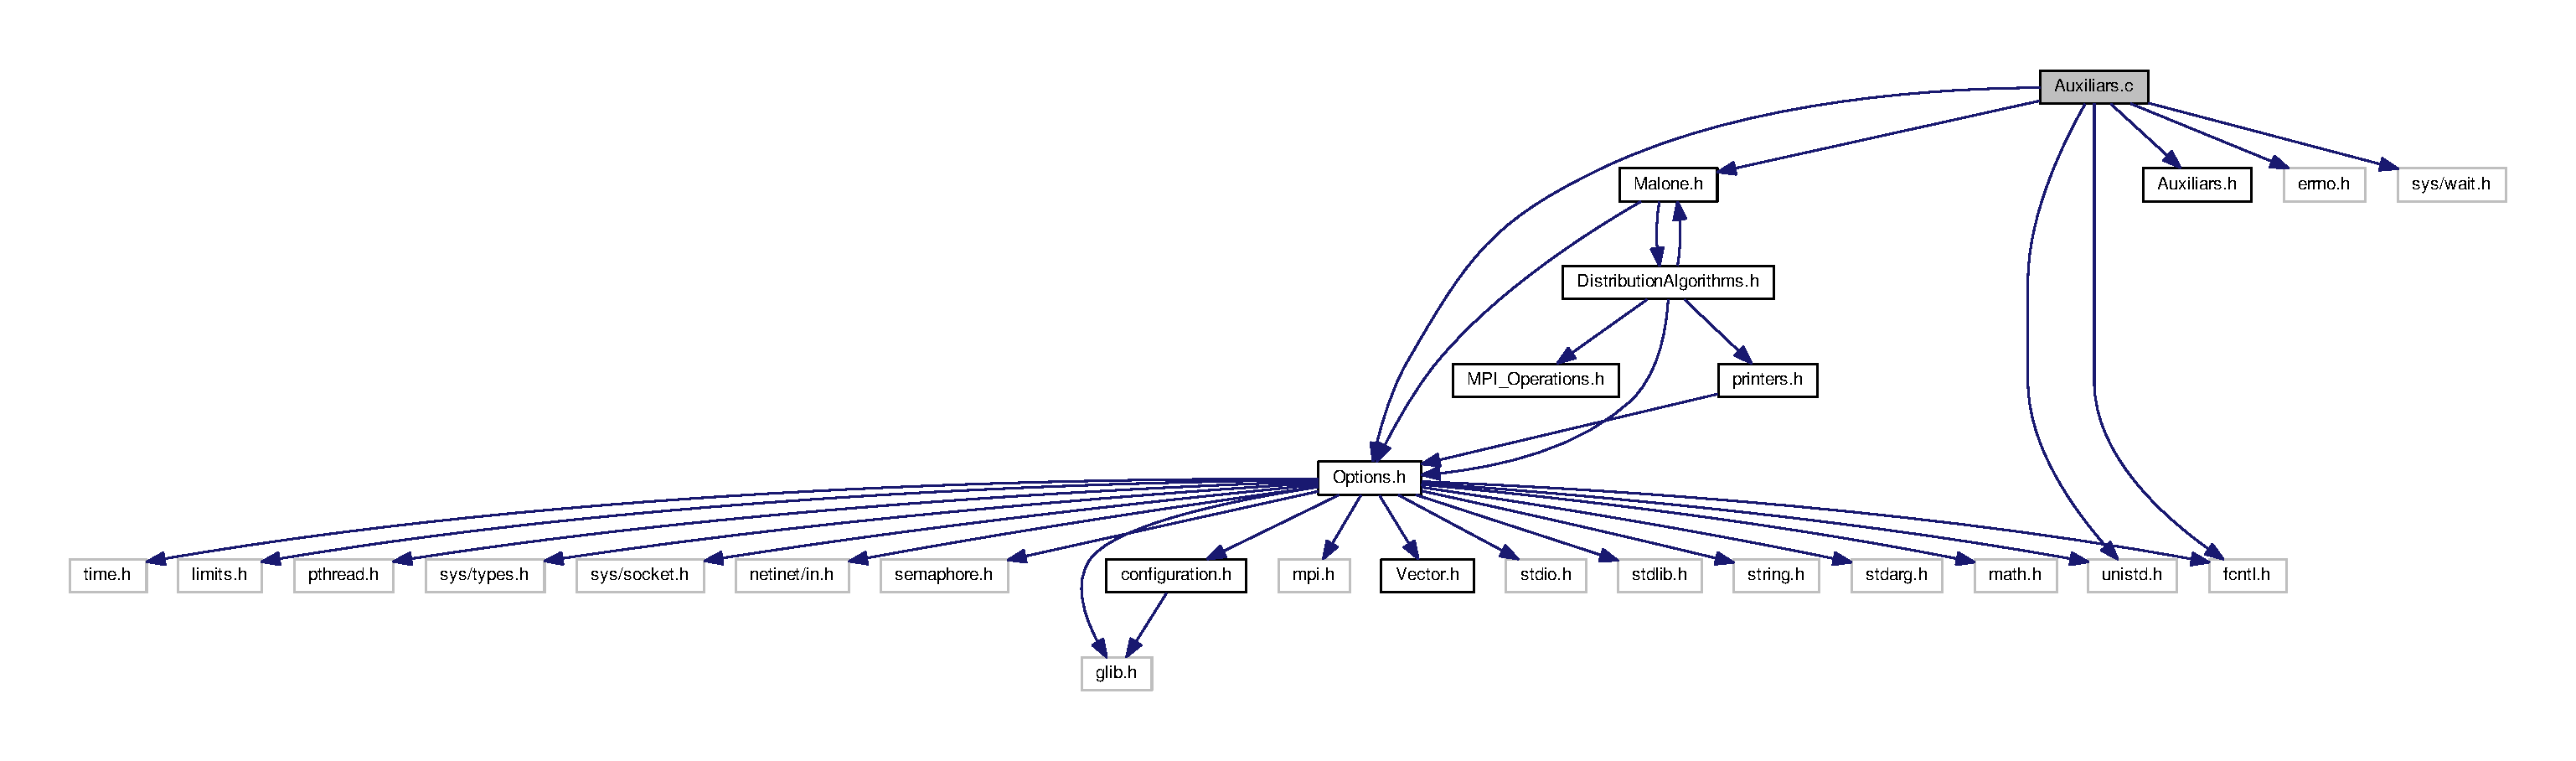
\includegraphics[width=350pt]{Auxiliars_8c__incl}
\end{center}
\end{figure}
\subsection*{Macros}
\begin{DoxyCompactItemize}
\item 
\#define \hyperlink{Auxiliars_8c_a86cb15faafedbfea31f54519d6940bba}{S\-L\-E\-E\-P\-\_\-\-F\-O\-R\-\_\-\-D\-E\-B\-U\-G}~0
\end{DoxyCompactItemize}
\subsection*{Functions}
\begin{DoxyCompactItemize}
\item 
void \hyperlink{Auxiliars_8c_a10491c96545ab6d0b126d2ca0db07cc6}{initialize\-\_\-auxiliars} ()
\item 
void \hyperlink{Auxiliars_8c_aad2abc7509dca3a174711497c2a2bbe4}{initialize\-Execution\-Map} (int n\-Mutants, int n\-Tests)
\item 
void \hyperlink{Auxiliars_8c_a7387501825c9e531f32281f0dcf07e07}{initialize\-Equivalent\-Map} (int n\-Mutants, int n\-Tests)
\item 
void \hyperlink{Auxiliars_8c_a07ed422b9084fb6a2fc2edb155ae590b}{redirect\-\_\-stdout} (char $\ast$str\-File)
\item 
int \hyperlink{Auxiliars_8c_ad524f269a2713fec2f64053c3704503b}{getenv\-\_\-int} (char $\ast$str\-Key)
\item 
long int \hyperlink{Auxiliars_8c_a60ab9fcbd72061289ed7af622754751b}{get\-Tick} ()
\item 
void \hyperlink{Auxiliars_8c_a0021dd07c447d6eecf839803f987b7c9}{add\-Result\-Index} (\hyperlink{structT__stTestList}{T\-\_\-st\-Test\-List} $\ast$p\-Test\-List, int n\-Index, const char $\ast$t, double d\-Time, int n\-Kill)
\item 
int \hyperlink{Auxiliars_8c_a6d20a5a58c64584accdeb1a904de9d83}{add\-Result} (\hyperlink{structT__stTestList}{T\-\_\-st\-Test\-List} $\ast$p\-Test\-List, const char $\ast$t, double d\-Time, int n\-Kill)
\item 
char $\ast$ \hyperlink{Auxiliars_8c_a6fb95aaf1a67c0dfc9e35416a96e58aa}{replace\-\_\-char} (const char $\ast$s, char ch, const char $\ast$repl)
\item 
char $\ast$ \hyperlink{Auxiliars_8c_a59689ac62cb991f149d59ff57f678550}{replace} (char const $\ast$const original, char const $\ast$const pattern, char const $\ast$const replacement)
\item 
char $\ast$ \hyperlink{Auxiliars_8c_a94eb643b244f2e7018d5a205b18cd4dc}{build\-Exe\-Line\-\_\-\-Stand\-Alone} (int n\-Index\-Mutant, int n\-Index\-Test, int n\-Original\-Mode)
\item 
char $\ast$ \hyperlink{Auxiliars_8c_a82109f9207eb5c668dcffd36565eaee7}{build\-Exe\-Line\-\_\-general} (int n\-Index\-Mutant, int n\-Index\-Test, int n\-Original\-Mode)
\item 
char $\ast$ \hyperlink{Auxiliars_8c_a89d711e5c117f1a990a8cf5e5c8630dc}{build\-Exe\-Line} (int n\-Index\-Mutant, int n\-Index\-Test, int n\-Original\-Mode)
\item 
char $\ast$ \hyperlink{Auxiliars_8c_aac97a075ec4d2647a6f281d3ef207202}{build\-Equiv\-Line} (int n\-Index\-Mutant, int n\-Original\-Mode)
\item 
char $\ast$ \hyperlink{Auxiliars_8c_abf20f0d0256aca4acc21a8bcef943aa2}{generate\-Compilation\-Line} (int n\-Index\-Mutant, int n\-Original\-Mode)
\item 
int \hyperlink{Auxiliars_8c_ad977bb957ddd724b9dd590e37d9fe093}{is\-Mutant\-Allocated} (int n\-Index\-Mutant)
\item 
int \hyperlink{Auxiliars_8c_a3ac75c1ea5af10a333cbda886d5b486d}{alloc\-Mutant} (int n\-Index\-Mutant)
\item 
void \hyperlink{Auxiliars_8c_a3b80d6dfc602edb25b80149fffe6ea9b}{insert\-Mutant} (\hyperlink{structT__stMutant}{T\-\_\-st\-Mutant} $\ast$p\-Mutant, int n\-Index\-Mutant)
\item 
void \hyperlink{Auxiliars_8c_ae868349a1b9962bef735c645c8af8429}{insert\-Mutant\-Test\-By\-Test} (\hyperlink{structT__stMutant}{T\-\_\-st\-Mutant} $\ast$p\-Mutant, int n\-Index\-Mutant, int n\-Worker\-Source)
\item 
int \hyperlink{Auxiliars_8c_afa2214923ca27bb087ebe0622ba7c152}{insert\-Test\-Result} (int n\-Mutant, int n\-Test, \hyperlink{structT__stTestInfo}{T\-\_\-st\-Test\-Info} $\ast$p\-Test)
\item 
int \hyperlink{Auxiliars_8c_a468c24e305d956cf0bb31debf9ff8a97}{insert\-Test\-Result\-\_\-unsorted} (int n\-Mutant, int n\-Test, \hyperlink{structT__stTestInfo}{T\-\_\-st\-Test\-Info} $\ast$p\-Test)
\item 
void \hyperlink{Auxiliars_8c_a146a12561b1a6fdedea1505ac4434faa}{insert\-Full\-Mutant\-Info} (int n\-Mutant, int n\-Mutant\-State, \hyperlink{structT__stTestList}{T\-\_\-st\-Test\-List} $\ast$p\-List)
\item 
int \hyperlink{Auxiliars_8c_a483eea21188eae7d531a113493aacd6b}{check\-Test\-Result} (\hyperlink{structT__stTestInfo}{T\-\_\-st\-Test\-Info} $\ast$p\-Test)
\item 
int \hyperlink{Auxiliars_8c_a438dd8b30a1f8b16fd956363f6909f29}{read\-Test\-Suite} ()
\item 
int \hyperlink{Auxiliars_8c_a1676fd50e6015c0f173b606f30b20127}{check\-Test\-Result\-Original} (\hyperlink{structT__stTestInfo}{T\-\_\-st\-Test\-Info} $\ast$p\-Test)
\item 
int \hyperlink{Auxiliars_8c_aa18130a85476ab3847ee9eb448fc4f03}{check\-Result\-Original} (int n\-Index\-Test, const char $\ast$str\-Result)
\item 
int \hyperlink{Auxiliars_8c_ac65810d8fde88b1a003403d3894e070e}{get\-Original\-Time} (\hyperlink{structT__stTestList}{T\-\_\-st\-Test\-List} $\ast$p\-List, int n\-Test)
\item 
int \hyperlink{Auxiliars_8c_a83dd3e45bbd9220ce41c2a2785ee2571}{check\-Result} (int n\-Index\-Test, const char $\ast$str\-Result)
\item 
\hyperlink{structT__stTestInfo}{T\-\_\-st\-Test\-Info} $\ast$ \hyperlink{Auxiliars_8c_a256f1dad89862377930e90a792b8e37d}{create\-Test} (int n\-Index\-Test, char $\ast$str\-Result, double d\-Time, int n\-Kill)
\item 
int \hyperlink{Auxiliars_8c_a5891dfe1066ac082980db1c3eb4c9f2c}{pretty\-Print} (int n\-Index, int n\-Total, int n\-Ant\-Prog)
\item 
void \hyperlink{Auxiliars_8c_ac08052e787477c50ef64b7ab0d7f1424}{show\-Debug\-Options} ()
\item 
int \hyperlink{Auxiliars_8c_a9fc952cf76aa8896184df882c33ed1c8}{is\-Enabled\-Aux\-Log} ()
\item 
int \hyperlink{Auxiliars_8c_a928b1da945af8413e422d1749058d33a}{file\-\_\-exist} (char $\ast$filename)
\item 
int \hyperlink{Auxiliars_8c_adcab8832f40183a4b4db8df7666bb42d}{dir\-\_\-exist} (const char $\ast$d)
\item 
void \hyperlink{Auxiliars_8c_a572fc7e90a3041bc8c17d3f23ad0a78d}{recursive\-\_\-mkdir} (char $\ast$path)
\item 
F\-I\-L\-E $\ast$ \hyperlink{Auxiliars_8c_a60db6d4d611a750ba6e19774ac2bcebb}{fopen\-\_\-mkdir} (char $\ast$path, char $\ast$mode)
\item 
int \hyperlink{Auxiliars_8c_a3201f70287d7dcf94efb84b3629deaf0}{generate\-Res\-Folder} ()
\item 
void \hyperlink{Auxiliars_8c_a41d4d001d9bf9a77465ed907374e0658}{copy} (char $\ast$source, char $\ast$dest)
\item 
void \hyperlink{Auxiliars_8c_af1f1971eb763b91534b6d0037b284193}{save\-Config\-And\-Environment\-Files} ()
\item 
char $\ast$ \hyperlink{Auxiliars_8c_a312b37675e7e147fb30b0cb53d7d8479}{exec\-Command\-Line} (const char $\ast$fmt,...)
\item 
\hyperlink{structMutantList}{Mutant\-List} $\ast$ \hyperlink{Auxiliars_8c_af0f8d130a0e61d129d7173fdada44943}{generate\-Clean\-Mutant\-List} (int n\-Mutants)
\item 
void \hyperlink{Auxiliars_8c_a3abc72bb2b5e7aa536901b5c47dd146f}{free\-Mutant\-List} (\hyperlink{structMutantList}{Mutant\-List} $\ast$p\-List)
\item 
int \hyperlink{Auxiliars_8c_af3d2268d78c36203c367ad1fe581743f}{is\-Enabled\-Debug\-Main\-Command\-Log} ()
\end{DoxyCompactItemize}


\subsection{Macro Definition Documentation}
\hypertarget{Auxiliars_8c_a86cb15faafedbfea31f54519d6940bba}{\index{Auxiliars.\-c@{Auxiliars.\-c}!S\-L\-E\-E\-P\-\_\-\-F\-O\-R\-\_\-\-D\-E\-B\-U\-G@{S\-L\-E\-E\-P\-\_\-\-F\-O\-R\-\_\-\-D\-E\-B\-U\-G}}
\index{S\-L\-E\-E\-P\-\_\-\-F\-O\-R\-\_\-\-D\-E\-B\-U\-G@{S\-L\-E\-E\-P\-\_\-\-F\-O\-R\-\_\-\-D\-E\-B\-U\-G}!Auxiliars.c@{Auxiliars.\-c}}
\subsubsection[{S\-L\-E\-E\-P\-\_\-\-F\-O\-R\-\_\-\-D\-E\-B\-U\-G}]{\setlength{\rightskip}{0pt plus 5cm}\#define S\-L\-E\-E\-P\-\_\-\-F\-O\-R\-\_\-\-D\-E\-B\-U\-G~0}}\label{Auxiliars_8c_a86cb15faafedbfea31f54519d6940bba}


\subsection{Function Documentation}
\hypertarget{Auxiliars_8c_a6d20a5a58c64584accdeb1a904de9d83}{\index{Auxiliars.\-c@{Auxiliars.\-c}!add\-Result@{add\-Result}}
\index{add\-Result@{add\-Result}!Auxiliars.c@{Auxiliars.\-c}}
\subsubsection[{add\-Result}]{\setlength{\rightskip}{0pt plus 5cm}int add\-Result (
\begin{DoxyParamCaption}
\item[{{\bf T\-\_\-st\-Test\-List} $\ast$}]{p\-Test\-List, }
\item[{const char $\ast$}]{t, }
\item[{double}]{d\-Time, }
\item[{int}]{n\-Kill}
\end{DoxyParamCaption}
)}}\label{Auxiliars_8c_a6d20a5a58c64584accdeb1a904de9d83}
\hypertarget{Auxiliars_8c_a0021dd07c447d6eecf839803f987b7c9}{\index{Auxiliars.\-c@{Auxiliars.\-c}!add\-Result\-Index@{add\-Result\-Index}}
\index{add\-Result\-Index@{add\-Result\-Index}!Auxiliars.c@{Auxiliars.\-c}}
\subsubsection[{add\-Result\-Index}]{\setlength{\rightskip}{0pt plus 5cm}void add\-Result\-Index (
\begin{DoxyParamCaption}
\item[{{\bf T\-\_\-st\-Test\-List} $\ast$}]{p\-Test\-List, }
\item[{int}]{n\-Index, }
\item[{const char $\ast$}]{t, }
\item[{double}]{d\-Time, }
\item[{int}]{n\-Kill}
\end{DoxyParamCaption}
)}}\label{Auxiliars_8c_a0021dd07c447d6eecf839803f987b7c9}
\hypertarget{Auxiliars_8c_a3ac75c1ea5af10a333cbda886d5b486d}{\index{Auxiliars.\-c@{Auxiliars.\-c}!alloc\-Mutant@{alloc\-Mutant}}
\index{alloc\-Mutant@{alloc\-Mutant}!Auxiliars.c@{Auxiliars.\-c}}
\subsubsection[{alloc\-Mutant}]{\setlength{\rightskip}{0pt plus 5cm}int alloc\-Mutant (
\begin{DoxyParamCaption}
\item[{int}]{n\-Index\-Mutant}
\end{DoxyParamCaption}
)}}\label{Auxiliars_8c_a3ac75c1ea5af10a333cbda886d5b486d}


Here is the call graph for this function\-:\nopagebreak
\begin{figure}[H]
\begin{center}
\leavevmode
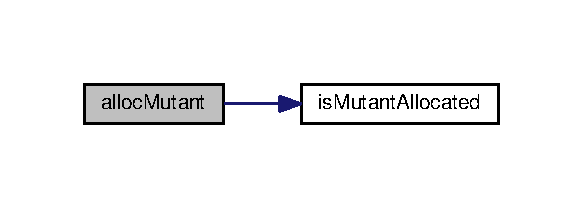
\includegraphics[width=280pt]{Auxiliars_8c_a3ac75c1ea5af10a333cbda886d5b486d_cgraph}
\end{center}
\end{figure}


\hypertarget{Auxiliars_8c_aac97a075ec4d2647a6f281d3ef207202}{\index{Auxiliars.\-c@{Auxiliars.\-c}!build\-Equiv\-Line@{build\-Equiv\-Line}}
\index{build\-Equiv\-Line@{build\-Equiv\-Line}!Auxiliars.c@{Auxiliars.\-c}}
\subsubsection[{build\-Equiv\-Line}]{\setlength{\rightskip}{0pt plus 5cm}char$\ast$ build\-Equiv\-Line (
\begin{DoxyParamCaption}
\item[{int}]{n\-Index\-Mutant, }
\item[{int}]{n\-Original\-Mode}
\end{DoxyParamCaption}
)}}\label{Auxiliars_8c_aac97a075ec4d2647a6f281d3ef207202}


Here is the call graph for this function\-:\nopagebreak
\begin{figure}[H]
\begin{center}
\leavevmode
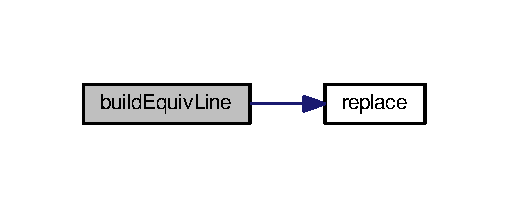
\includegraphics[width=244pt]{Auxiliars_8c_aac97a075ec4d2647a6f281d3ef207202_cgraph}
\end{center}
\end{figure}


\hypertarget{Auxiliars_8c_a89d711e5c117f1a990a8cf5e5c8630dc}{\index{Auxiliars.\-c@{Auxiliars.\-c}!build\-Exe\-Line@{build\-Exe\-Line}}
\index{build\-Exe\-Line@{build\-Exe\-Line}!Auxiliars.c@{Auxiliars.\-c}}
\subsubsection[{build\-Exe\-Line}]{\setlength{\rightskip}{0pt plus 5cm}char$\ast$ build\-Exe\-Line (
\begin{DoxyParamCaption}
\item[{int}]{n\-Index\-Mutant, }
\item[{int}]{n\-Index\-Test, }
\item[{int}]{n\-Original\-Mode}
\end{DoxyParamCaption}
)}}\label{Auxiliars_8c_a89d711e5c117f1a990a8cf5e5c8630dc}


Here is the call graph for this function\-:\nopagebreak
\begin{figure}[H]
\begin{center}
\leavevmode
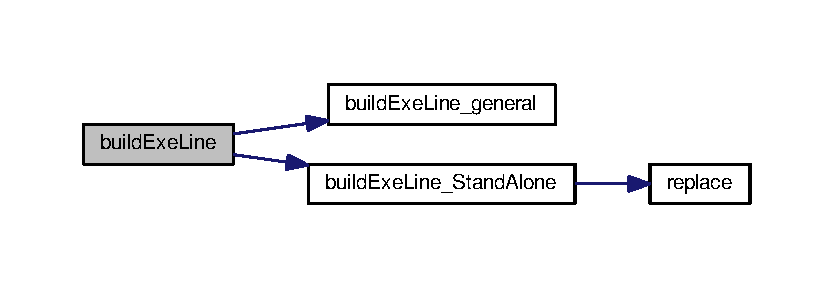
\includegraphics[width=350pt]{Auxiliars_8c_a89d711e5c117f1a990a8cf5e5c8630dc_cgraph}
\end{center}
\end{figure}


\hypertarget{Auxiliars_8c_a82109f9207eb5c668dcffd36565eaee7}{\index{Auxiliars.\-c@{Auxiliars.\-c}!build\-Exe\-Line\-\_\-general@{build\-Exe\-Line\-\_\-general}}
\index{build\-Exe\-Line\-\_\-general@{build\-Exe\-Line\-\_\-general}!Auxiliars.c@{Auxiliars.\-c}}
\subsubsection[{build\-Exe\-Line\-\_\-general}]{\setlength{\rightskip}{0pt plus 5cm}char$\ast$ build\-Exe\-Line\-\_\-general (
\begin{DoxyParamCaption}
\item[{int}]{n\-Index\-Mutant, }
\item[{int}]{n\-Index\-Test, }
\item[{int}]{n\-Original\-Mode}
\end{DoxyParamCaption}
)}}\label{Auxiliars_8c_a82109f9207eb5c668dcffd36565eaee7}
\hypertarget{Auxiliars_8c_a94eb643b244f2e7018d5a205b18cd4dc}{\index{Auxiliars.\-c@{Auxiliars.\-c}!build\-Exe\-Line\-\_\-\-Stand\-Alone@{build\-Exe\-Line\-\_\-\-Stand\-Alone}}
\index{build\-Exe\-Line\-\_\-\-Stand\-Alone@{build\-Exe\-Line\-\_\-\-Stand\-Alone}!Auxiliars.c@{Auxiliars.\-c}}
\subsubsection[{build\-Exe\-Line\-\_\-\-Stand\-Alone}]{\setlength{\rightskip}{0pt plus 5cm}char$\ast$ build\-Exe\-Line\-\_\-\-Stand\-Alone (
\begin{DoxyParamCaption}
\item[{int}]{n\-Index\-Mutant, }
\item[{int}]{n\-Index\-Test, }
\item[{int}]{n\-Original\-Mode}
\end{DoxyParamCaption}
)}}\label{Auxiliars_8c_a94eb643b244f2e7018d5a205b18cd4dc}


Here is the call graph for this function\-:\nopagebreak
\begin{figure}[H]
\begin{center}
\leavevmode
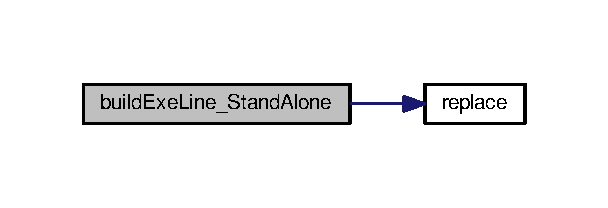
\includegraphics[width=292pt]{Auxiliars_8c_a94eb643b244f2e7018d5a205b18cd4dc_cgraph}
\end{center}
\end{figure}


\hypertarget{Auxiliars_8c_a83dd3e45bbd9220ce41c2a2785ee2571}{\index{Auxiliars.\-c@{Auxiliars.\-c}!check\-Result@{check\-Result}}
\index{check\-Result@{check\-Result}!Auxiliars.c@{Auxiliars.\-c}}
\subsubsection[{check\-Result}]{\setlength{\rightskip}{0pt plus 5cm}int check\-Result (
\begin{DoxyParamCaption}
\item[{int}]{n\-Index\-Test, }
\item[{const char $\ast$}]{str\-Result}
\end{DoxyParamCaption}
)}}\label{Auxiliars_8c_a83dd3e45bbd9220ce41c2a2785ee2571}
\hypertarget{Auxiliars_8c_aa18130a85476ab3847ee9eb448fc4f03}{\index{Auxiliars.\-c@{Auxiliars.\-c}!check\-Result\-Original@{check\-Result\-Original}}
\index{check\-Result\-Original@{check\-Result\-Original}!Auxiliars.c@{Auxiliars.\-c}}
\subsubsection[{check\-Result\-Original}]{\setlength{\rightskip}{0pt plus 5cm}int check\-Result\-Original (
\begin{DoxyParamCaption}
\item[{int}]{n\-Index\-Test, }
\item[{const char $\ast$}]{str\-Result}
\end{DoxyParamCaption}
)}}\label{Auxiliars_8c_aa18130a85476ab3847ee9eb448fc4f03}


Here is the call graph for this function\-:\nopagebreak
\begin{figure}[H]
\begin{center}
\leavevmode
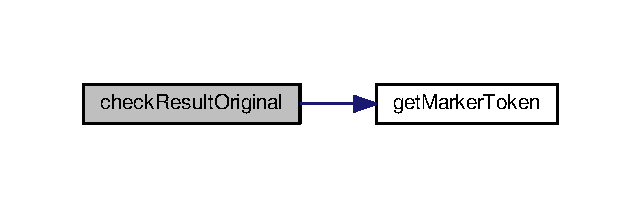
\includegraphics[width=308pt]{Auxiliars_8c_aa18130a85476ab3847ee9eb448fc4f03_cgraph}
\end{center}
\end{figure}


\hypertarget{Auxiliars_8c_a483eea21188eae7d531a113493aacd6b}{\index{Auxiliars.\-c@{Auxiliars.\-c}!check\-Test\-Result@{check\-Test\-Result}}
\index{check\-Test\-Result@{check\-Test\-Result}!Auxiliars.c@{Auxiliars.\-c}}
\subsubsection[{check\-Test\-Result}]{\setlength{\rightskip}{0pt plus 5cm}int check\-Test\-Result (
\begin{DoxyParamCaption}
\item[{{\bf T\-\_\-st\-Test\-Info} $\ast$}]{p\-Test}
\end{DoxyParamCaption}
)}}\label{Auxiliars_8c_a483eea21188eae7d531a113493aacd6b}


Here is the call graph for this function\-:\nopagebreak
\begin{figure}[H]
\begin{center}
\leavevmode
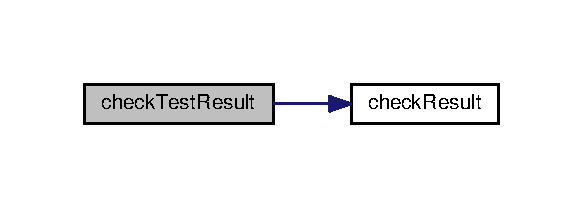
\includegraphics[width=280pt]{Auxiliars_8c_a483eea21188eae7d531a113493aacd6b_cgraph}
\end{center}
\end{figure}


\hypertarget{Auxiliars_8c_a1676fd50e6015c0f173b606f30b20127}{\index{Auxiliars.\-c@{Auxiliars.\-c}!check\-Test\-Result\-Original@{check\-Test\-Result\-Original}}
\index{check\-Test\-Result\-Original@{check\-Test\-Result\-Original}!Auxiliars.c@{Auxiliars.\-c}}
\subsubsection[{check\-Test\-Result\-Original}]{\setlength{\rightskip}{0pt plus 5cm}int check\-Test\-Result\-Original (
\begin{DoxyParamCaption}
\item[{{\bf T\-\_\-st\-Test\-Info} $\ast$}]{p\-Test}
\end{DoxyParamCaption}
)}}\label{Auxiliars_8c_a1676fd50e6015c0f173b606f30b20127}


Here is the call graph for this function\-:\nopagebreak
\begin{figure}[H]
\begin{center}
\leavevmode
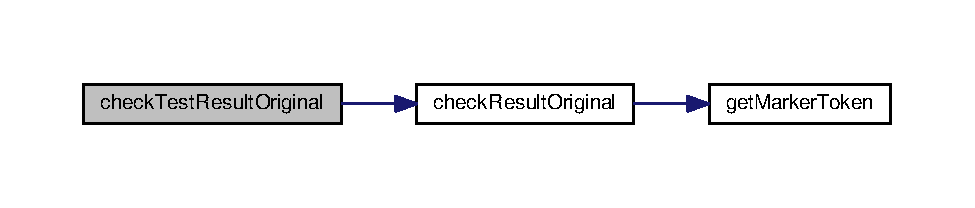
\includegraphics[width=350pt]{Auxiliars_8c_a1676fd50e6015c0f173b606f30b20127_cgraph}
\end{center}
\end{figure}


\hypertarget{Auxiliars_8c_a41d4d001d9bf9a77465ed907374e0658}{\index{Auxiliars.\-c@{Auxiliars.\-c}!copy@{copy}}
\index{copy@{copy}!Auxiliars.c@{Auxiliars.\-c}}
\subsubsection[{copy}]{\setlength{\rightskip}{0pt plus 5cm}void copy (
\begin{DoxyParamCaption}
\item[{char $\ast$}]{source, }
\item[{char $\ast$}]{dest}
\end{DoxyParamCaption}
)}}\label{Auxiliars_8c_a41d4d001d9bf9a77465ed907374e0658}
\hypertarget{Auxiliars_8c_a256f1dad89862377930e90a792b8e37d}{\index{Auxiliars.\-c@{Auxiliars.\-c}!create\-Test@{create\-Test}}
\index{create\-Test@{create\-Test}!Auxiliars.c@{Auxiliars.\-c}}
\subsubsection[{create\-Test}]{\setlength{\rightskip}{0pt plus 5cm}{\bf T\-\_\-st\-Test\-Info}$\ast$ create\-Test (
\begin{DoxyParamCaption}
\item[{int}]{n\-Index\-Test, }
\item[{char $\ast$}]{str\-Result, }
\item[{double}]{d\-Time, }
\item[{int}]{n\-Kill}
\end{DoxyParamCaption}
)}}\label{Auxiliars_8c_a256f1dad89862377930e90a792b8e37d}
\hypertarget{Auxiliars_8c_adcab8832f40183a4b4db8df7666bb42d}{\index{Auxiliars.\-c@{Auxiliars.\-c}!dir\-\_\-exist@{dir\-\_\-exist}}
\index{dir\-\_\-exist@{dir\-\_\-exist}!Auxiliars.c@{Auxiliars.\-c}}
\subsubsection[{dir\-\_\-exist}]{\setlength{\rightskip}{0pt plus 5cm}int dir\-\_\-exist (
\begin{DoxyParamCaption}
\item[{const char $\ast$}]{d}
\end{DoxyParamCaption}
)}}\label{Auxiliars_8c_adcab8832f40183a4b4db8df7666bb42d}
\hypertarget{Auxiliars_8c_a312b37675e7e147fb30b0cb53d7d8479}{\index{Auxiliars.\-c@{Auxiliars.\-c}!exec\-Command\-Line@{exec\-Command\-Line}}
\index{exec\-Command\-Line@{exec\-Command\-Line}!Auxiliars.c@{Auxiliars.\-c}}
\subsubsection[{exec\-Command\-Line}]{\setlength{\rightskip}{0pt plus 5cm}char$\ast$ exec\-Command\-Line (
\begin{DoxyParamCaption}
\item[{const char $\ast$}]{fmt, }
\item[{}]{...}
\end{DoxyParamCaption}
)}}\label{Auxiliars_8c_a312b37675e7e147fb30b0cb53d7d8479}
\hypertarget{Auxiliars_8c_a928b1da945af8413e422d1749058d33a}{\index{Auxiliars.\-c@{Auxiliars.\-c}!file\-\_\-exist@{file\-\_\-exist}}
\index{file\-\_\-exist@{file\-\_\-exist}!Auxiliars.c@{Auxiliars.\-c}}
\subsubsection[{file\-\_\-exist}]{\setlength{\rightskip}{0pt plus 5cm}int file\-\_\-exist (
\begin{DoxyParamCaption}
\item[{char $\ast$}]{filename}
\end{DoxyParamCaption}
)}}\label{Auxiliars_8c_a928b1da945af8413e422d1749058d33a}
\hypertarget{Auxiliars_8c_a60db6d4d611a750ba6e19774ac2bcebb}{\index{Auxiliars.\-c@{Auxiliars.\-c}!fopen\-\_\-mkdir@{fopen\-\_\-mkdir}}
\index{fopen\-\_\-mkdir@{fopen\-\_\-mkdir}!Auxiliars.c@{Auxiliars.\-c}}
\subsubsection[{fopen\-\_\-mkdir}]{\setlength{\rightskip}{0pt plus 5cm}F\-I\-L\-E$\ast$ fopen\-\_\-mkdir (
\begin{DoxyParamCaption}
\item[{char $\ast$}]{path, }
\item[{char $\ast$}]{mode}
\end{DoxyParamCaption}
)}}\label{Auxiliars_8c_a60db6d4d611a750ba6e19774ac2bcebb}


Here is the call graph for this function\-:\nopagebreak
\begin{figure}[H]
\begin{center}
\leavevmode
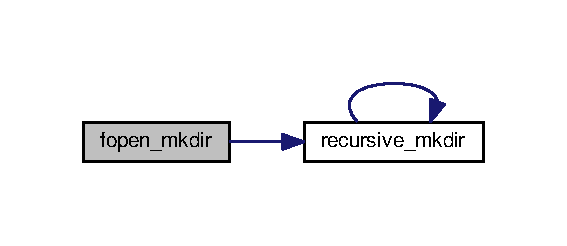
\includegraphics[width=272pt]{Auxiliars_8c_a60db6d4d611a750ba6e19774ac2bcebb_cgraph}
\end{center}
\end{figure}


\hypertarget{Auxiliars_8c_a3abc72bb2b5e7aa536901b5c47dd146f}{\index{Auxiliars.\-c@{Auxiliars.\-c}!free\-Mutant\-List@{free\-Mutant\-List}}
\index{free\-Mutant\-List@{free\-Mutant\-List}!Auxiliars.c@{Auxiliars.\-c}}
\subsubsection[{free\-Mutant\-List}]{\setlength{\rightskip}{0pt plus 5cm}void free\-Mutant\-List (
\begin{DoxyParamCaption}
\item[{{\bf Mutant\-List} $\ast$}]{p\-List}
\end{DoxyParamCaption}
)}}\label{Auxiliars_8c_a3abc72bb2b5e7aa536901b5c47dd146f}
\hypertarget{Auxiliars_8c_af0f8d130a0e61d129d7173fdada44943}{\index{Auxiliars.\-c@{Auxiliars.\-c}!generate\-Clean\-Mutant\-List@{generate\-Clean\-Mutant\-List}}
\index{generate\-Clean\-Mutant\-List@{generate\-Clean\-Mutant\-List}!Auxiliars.c@{Auxiliars.\-c}}
\subsubsection[{generate\-Clean\-Mutant\-List}]{\setlength{\rightskip}{0pt plus 5cm}{\bf Mutant\-List}$\ast$ generate\-Clean\-Mutant\-List (
\begin{DoxyParamCaption}
\item[{int}]{n\-Mutants}
\end{DoxyParamCaption}
)}}\label{Auxiliars_8c_af0f8d130a0e61d129d7173fdada44943}
\hypertarget{Auxiliars_8c_abf20f0d0256aca4acc21a8bcef943aa2}{\index{Auxiliars.\-c@{Auxiliars.\-c}!generate\-Compilation\-Line@{generate\-Compilation\-Line}}
\index{generate\-Compilation\-Line@{generate\-Compilation\-Line}!Auxiliars.c@{Auxiliars.\-c}}
\subsubsection[{generate\-Compilation\-Line}]{\setlength{\rightskip}{0pt plus 5cm}char$\ast$ generate\-Compilation\-Line (
\begin{DoxyParamCaption}
\item[{int}]{n\-Index\-Mutant, }
\item[{int}]{n\-Original\-Mode}
\end{DoxyParamCaption}
)}}\label{Auxiliars_8c_abf20f0d0256aca4acc21a8bcef943aa2}


Here is the call graph for this function\-:\nopagebreak
\begin{figure}[H]
\begin{center}
\leavevmode
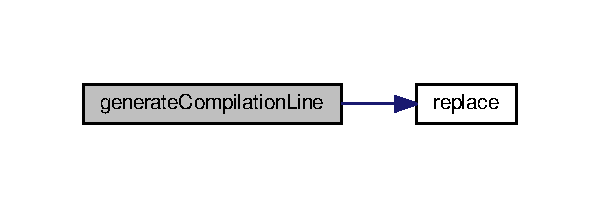
\includegraphics[width=288pt]{Auxiliars_8c_abf20f0d0256aca4acc21a8bcef943aa2_cgraph}
\end{center}
\end{figure}


\hypertarget{Auxiliars_8c_a3201f70287d7dcf94efb84b3629deaf0}{\index{Auxiliars.\-c@{Auxiliars.\-c}!generate\-Res\-Folder@{generate\-Res\-Folder}}
\index{generate\-Res\-Folder@{generate\-Res\-Folder}!Auxiliars.c@{Auxiliars.\-c}}
\subsubsection[{generate\-Res\-Folder}]{\setlength{\rightskip}{0pt plus 5cm}int generate\-Res\-Folder (
\begin{DoxyParamCaption}
{}
\end{DoxyParamCaption}
)}}\label{Auxiliars_8c_a3201f70287d7dcf94efb84b3629deaf0}


Here is the call graph for this function\-:\nopagebreak
\begin{figure}[H]
\begin{center}
\leavevmode
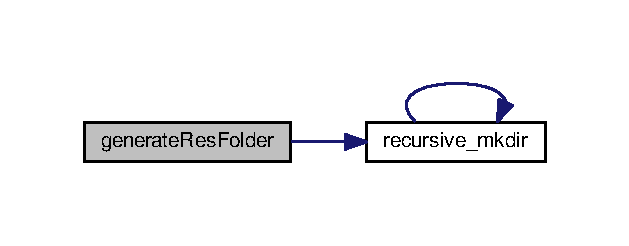
\includegraphics[width=302pt]{Auxiliars_8c_a3201f70287d7dcf94efb84b3629deaf0_cgraph}
\end{center}
\end{figure}


\hypertarget{Auxiliars_8c_ad524f269a2713fec2f64053c3704503b}{\index{Auxiliars.\-c@{Auxiliars.\-c}!getenv\-\_\-int@{getenv\-\_\-int}}
\index{getenv\-\_\-int@{getenv\-\_\-int}!Auxiliars.c@{Auxiliars.\-c}}
\subsubsection[{getenv\-\_\-int}]{\setlength{\rightskip}{0pt plus 5cm}int getenv\-\_\-int (
\begin{DoxyParamCaption}
\item[{char $\ast$}]{str\-Key}
\end{DoxyParamCaption}
)}}\label{Auxiliars_8c_ad524f269a2713fec2f64053c3704503b}
\hypertarget{Auxiliars_8c_ac65810d8fde88b1a003403d3894e070e}{\index{Auxiliars.\-c@{Auxiliars.\-c}!get\-Original\-Time@{get\-Original\-Time}}
\index{get\-Original\-Time@{get\-Original\-Time}!Auxiliars.c@{Auxiliars.\-c}}
\subsubsection[{get\-Original\-Time}]{\setlength{\rightskip}{0pt plus 5cm}int get\-Original\-Time (
\begin{DoxyParamCaption}
\item[{{\bf T\-\_\-st\-Test\-List} $\ast$}]{p\-List, }
\item[{int}]{n\-Test}
\end{DoxyParamCaption}
)}}\label{Auxiliars_8c_ac65810d8fde88b1a003403d3894e070e}
Get the execution time needed to apply the test over the original program 
\begin{DoxyParams}{Parameters}
{\em n\-Test} & \\
\hline
\end{DoxyParams}
\begin{DoxyReturn}{Returns}

\end{DoxyReturn}
\hypertarget{Auxiliars_8c_a60ab9fcbd72061289ed7af622754751b}{\index{Auxiliars.\-c@{Auxiliars.\-c}!get\-Tick@{get\-Tick}}
\index{get\-Tick@{get\-Tick}!Auxiliars.c@{Auxiliars.\-c}}
\subsubsection[{get\-Tick}]{\setlength{\rightskip}{0pt plus 5cm}long int get\-Tick (
\begin{DoxyParamCaption}
{}
\end{DoxyParamCaption}
)}}\label{Auxiliars_8c_a60ab9fcbd72061289ed7af622754751b}
\hypertarget{Auxiliars_8c_a10491c96545ab6d0b126d2ca0db07cc6}{\index{Auxiliars.\-c@{Auxiliars.\-c}!initialize\-\_\-auxiliars@{initialize\-\_\-auxiliars}}
\index{initialize\-\_\-auxiliars@{initialize\-\_\-auxiliars}!Auxiliars.c@{Auxiliars.\-c}}
\subsubsection[{initialize\-\_\-auxiliars}]{\setlength{\rightskip}{0pt plus 5cm}void initialize\-\_\-auxiliars (
\begin{DoxyParamCaption}
{}
\end{DoxyParamCaption}
)}}\label{Auxiliars_8c_a10491c96545ab6d0b126d2ca0db07cc6}
\hypertarget{Auxiliars_8c_a7387501825c9e531f32281f0dcf07e07}{\index{Auxiliars.\-c@{Auxiliars.\-c}!initialize\-Equivalent\-Map@{initialize\-Equivalent\-Map}}
\index{initialize\-Equivalent\-Map@{initialize\-Equivalent\-Map}!Auxiliars.c@{Auxiliars.\-c}}
\subsubsection[{initialize\-Equivalent\-Map}]{\setlength{\rightskip}{0pt plus 5cm}void initialize\-Equivalent\-Map (
\begin{DoxyParamCaption}
\item[{int}]{n\-Mutants, }
\item[{int}]{n\-Tests}
\end{DoxyParamCaption}
)}}\label{Auxiliars_8c_a7387501825c9e531f32281f0dcf07e07}
\hypertarget{Auxiliars_8c_aad2abc7509dca3a174711497c2a2bbe4}{\index{Auxiliars.\-c@{Auxiliars.\-c}!initialize\-Execution\-Map@{initialize\-Execution\-Map}}
\index{initialize\-Execution\-Map@{initialize\-Execution\-Map}!Auxiliars.c@{Auxiliars.\-c}}
\subsubsection[{initialize\-Execution\-Map}]{\setlength{\rightskip}{0pt plus 5cm}void initialize\-Execution\-Map (
\begin{DoxyParamCaption}
\item[{int}]{n\-Mutants, }
\item[{int}]{n\-Tests}
\end{DoxyParamCaption}
)}}\label{Auxiliars_8c_aad2abc7509dca3a174711497c2a2bbe4}
\hypertarget{Auxiliars_8c_a146a12561b1a6fdedea1505ac4434faa}{\index{Auxiliars.\-c@{Auxiliars.\-c}!insert\-Full\-Mutant\-Info@{insert\-Full\-Mutant\-Info}}
\index{insert\-Full\-Mutant\-Info@{insert\-Full\-Mutant\-Info}!Auxiliars.c@{Auxiliars.\-c}}
\subsubsection[{insert\-Full\-Mutant\-Info}]{\setlength{\rightskip}{0pt plus 5cm}void insert\-Full\-Mutant\-Info (
\begin{DoxyParamCaption}
\item[{int}]{n\-Mutant, }
\item[{int}]{n\-Mutant\-State, }
\item[{{\bf T\-\_\-st\-Test\-List} $\ast$}]{p\-List}
\end{DoxyParamCaption}
)}}\label{Auxiliars_8c_a146a12561b1a6fdedea1505ac4434faa}
\hypertarget{Auxiliars_8c_a3b80d6dfc602edb25b80149fffe6ea9b}{\index{Auxiliars.\-c@{Auxiliars.\-c}!insert\-Mutant@{insert\-Mutant}}
\index{insert\-Mutant@{insert\-Mutant}!Auxiliars.c@{Auxiliars.\-c}}
\subsubsection[{insert\-Mutant}]{\setlength{\rightskip}{0pt plus 5cm}void insert\-Mutant (
\begin{DoxyParamCaption}
\item[{{\bf T\-\_\-st\-Mutant} $\ast$}]{p\-Mutant, }
\item[{int}]{n\-Index\-Mutant}
\end{DoxyParamCaption}
)}}\label{Auxiliars_8c_a3b80d6dfc602edb25b80149fffe6ea9b}
\hypertarget{Auxiliars_8c_ae868349a1b9962bef735c645c8af8429}{\index{Auxiliars.\-c@{Auxiliars.\-c}!insert\-Mutant\-Test\-By\-Test@{insert\-Mutant\-Test\-By\-Test}}
\index{insert\-Mutant\-Test\-By\-Test@{insert\-Mutant\-Test\-By\-Test}!Auxiliars.c@{Auxiliars.\-c}}
\subsubsection[{insert\-Mutant\-Test\-By\-Test}]{\setlength{\rightskip}{0pt plus 5cm}void insert\-Mutant\-Test\-By\-Test (
\begin{DoxyParamCaption}
\item[{{\bf T\-\_\-st\-Mutant} $\ast$}]{p\-Mutant, }
\item[{int}]{n\-Index\-Mutant, }
\item[{int}]{n\-Worker\-Source}
\end{DoxyParamCaption}
)}}\label{Auxiliars_8c_ae868349a1b9962bef735c645c8af8429}


Here is the call graph for this function\-:\nopagebreak
\begin{figure}[H]
\begin{center}
\leavevmode
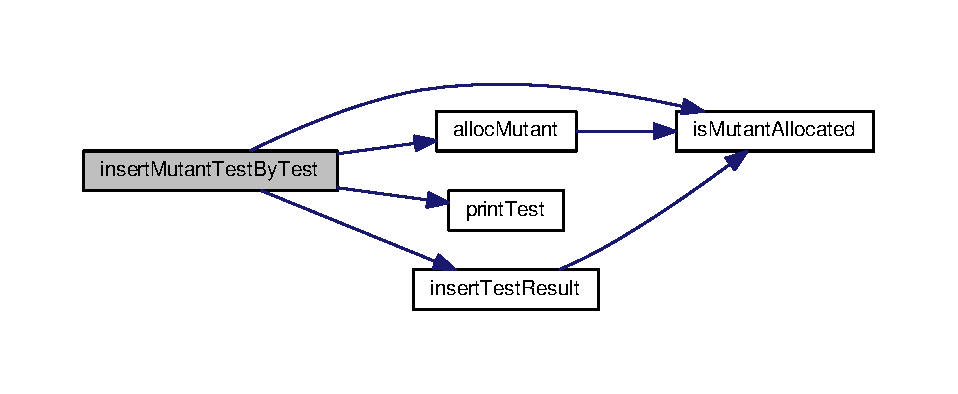
\includegraphics[width=350pt]{Auxiliars_8c_ae868349a1b9962bef735c645c8af8429_cgraph}
\end{center}
\end{figure}


\hypertarget{Auxiliars_8c_afa2214923ca27bb087ebe0622ba7c152}{\index{Auxiliars.\-c@{Auxiliars.\-c}!insert\-Test\-Result@{insert\-Test\-Result}}
\index{insert\-Test\-Result@{insert\-Test\-Result}!Auxiliars.c@{Auxiliars.\-c}}
\subsubsection[{insert\-Test\-Result}]{\setlength{\rightskip}{0pt plus 5cm}int insert\-Test\-Result (
\begin{DoxyParamCaption}
\item[{int}]{n\-Mutant, }
\item[{int}]{n\-Test, }
\item[{{\bf T\-\_\-st\-Test\-Info} $\ast$}]{p\-Test}
\end{DoxyParamCaption}
)}}\label{Auxiliars_8c_afa2214923ca27bb087ebe0622ba7c152}


Here is the call graph for this function\-:\nopagebreak
\begin{figure}[H]
\begin{center}
\leavevmode
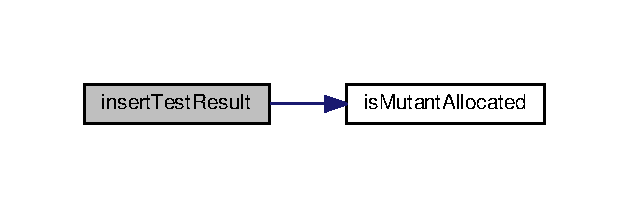
\includegraphics[width=302pt]{Auxiliars_8c_afa2214923ca27bb087ebe0622ba7c152_cgraph}
\end{center}
\end{figure}


\hypertarget{Auxiliars_8c_a468c24e305d956cf0bb31debf9ff8a97}{\index{Auxiliars.\-c@{Auxiliars.\-c}!insert\-Test\-Result\-\_\-unsorted@{insert\-Test\-Result\-\_\-unsorted}}
\index{insert\-Test\-Result\-\_\-unsorted@{insert\-Test\-Result\-\_\-unsorted}!Auxiliars.c@{Auxiliars.\-c}}
\subsubsection[{insert\-Test\-Result\-\_\-unsorted}]{\setlength{\rightskip}{0pt plus 5cm}int insert\-Test\-Result\-\_\-unsorted (
\begin{DoxyParamCaption}
\item[{int}]{n\-Mutant, }
\item[{int}]{n\-Test, }
\item[{{\bf T\-\_\-st\-Test\-Info} $\ast$}]{p\-Test}
\end{DoxyParamCaption}
)}}\label{Auxiliars_8c_a468c24e305d956cf0bb31debf9ff8a97}
This function is designed to insert a test in the first free position in the vector. The main diference with insert\-Result is related with the order. In this case we can have a test vector such \mbox{[}t2,t3,t5\mbox{]} since with insert\-Result we'd have \mbox{[}null,null,t2,t3,null,t5\mbox{]}. We have designed it to achieve a better performance 
\begin{DoxyParams}{Parameters}
{\em n\-Mutant} & Mutant where the test will be inserted \\
\hline
{\em p\-Test} & Test to insert \\
\hline
\end{DoxyParams}
\begin{DoxyReturn}{Returns}
0 if the mutant is not allocated 
\end{DoxyReturn}


Here is the call graph for this function\-:\nopagebreak
\begin{figure}[H]
\begin{center}
\leavevmode
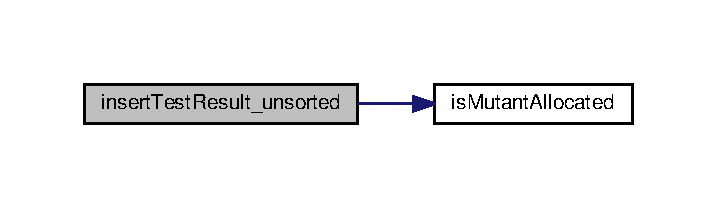
\includegraphics[width=344pt]{Auxiliars_8c_a468c24e305d956cf0bb31debf9ff8a97_cgraph}
\end{center}
\end{figure}


\hypertarget{Auxiliars_8c_a9fc952cf76aa8896184df882c33ed1c8}{\index{Auxiliars.\-c@{Auxiliars.\-c}!is\-Enabled\-Aux\-Log@{is\-Enabled\-Aux\-Log}}
\index{is\-Enabled\-Aux\-Log@{is\-Enabled\-Aux\-Log}!Auxiliars.c@{Auxiliars.\-c}}
\subsubsection[{is\-Enabled\-Aux\-Log}]{\setlength{\rightskip}{0pt plus 5cm}int is\-Enabled\-Aux\-Log (
\begin{DoxyParamCaption}
{}
\end{DoxyParamCaption}
)}}\label{Auxiliars_8c_a9fc952cf76aa8896184df882c33ed1c8}
\hypertarget{Auxiliars_8c_af3d2268d78c36203c367ad1fe581743f}{\index{Auxiliars.\-c@{Auxiliars.\-c}!is\-Enabled\-Debug\-Main\-Command\-Log@{is\-Enabled\-Debug\-Main\-Command\-Log}}
\index{is\-Enabled\-Debug\-Main\-Command\-Log@{is\-Enabled\-Debug\-Main\-Command\-Log}!Auxiliars.c@{Auxiliars.\-c}}
\subsubsection[{is\-Enabled\-Debug\-Main\-Command\-Log}]{\setlength{\rightskip}{0pt plus 5cm}int is\-Enabled\-Debug\-Main\-Command\-Log (
\begin{DoxyParamCaption}
{}
\end{DoxyParamCaption}
)}}\label{Auxiliars_8c_af3d2268d78c36203c367ad1fe581743f}
\hypertarget{Auxiliars_8c_ad977bb957ddd724b9dd590e37d9fe093}{\index{Auxiliars.\-c@{Auxiliars.\-c}!is\-Mutant\-Allocated@{is\-Mutant\-Allocated}}
\index{is\-Mutant\-Allocated@{is\-Mutant\-Allocated}!Auxiliars.c@{Auxiliars.\-c}}
\subsubsection[{is\-Mutant\-Allocated}]{\setlength{\rightskip}{0pt plus 5cm}int is\-Mutant\-Allocated (
\begin{DoxyParamCaption}
\item[{int}]{n\-Index\-Mutant}
\end{DoxyParamCaption}
)}}\label{Auxiliars_8c_ad977bb957ddd724b9dd590e37d9fe093}
\hypertarget{Auxiliars_8c_a5891dfe1066ac082980db1c3eb4c9f2c}{\index{Auxiliars.\-c@{Auxiliars.\-c}!pretty\-Print@{pretty\-Print}}
\index{pretty\-Print@{pretty\-Print}!Auxiliars.c@{Auxiliars.\-c}}
\subsubsection[{pretty\-Print}]{\setlength{\rightskip}{0pt plus 5cm}int pretty\-Print (
\begin{DoxyParamCaption}
\item[{int}]{n\-Index, }
\item[{int}]{n\-Total, }
\item[{int}]{n\-Ant\-Prog}
\end{DoxyParamCaption}
)}}\label{Auxiliars_8c_a5891dfe1066ac082980db1c3eb4c9f2c}
\hypertarget{Auxiliars_8c_a438dd8b30a1f8b16fd956363f6909f29}{\index{Auxiliars.\-c@{Auxiliars.\-c}!read\-Test\-Suite@{read\-Test\-Suite}}
\index{read\-Test\-Suite@{read\-Test\-Suite}!Auxiliars.c@{Auxiliars.\-c}}
\subsubsection[{read\-Test\-Suite}]{\setlength{\rightskip}{0pt plus 5cm}int read\-Test\-Suite (
\begin{DoxyParamCaption}
{}
\end{DoxyParamCaption}
)}}\label{Auxiliars_8c_a438dd8b30a1f8b16fd956363f6909f29}


Here is the call graph for this function\-:\nopagebreak
\begin{figure}[H]
\begin{center}
\leavevmode
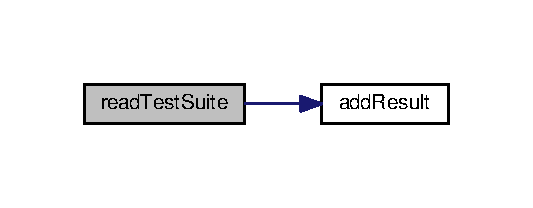
\includegraphics[width=256pt]{Auxiliars_8c_a438dd8b30a1f8b16fd956363f6909f29_cgraph}
\end{center}
\end{figure}


\hypertarget{Auxiliars_8c_a572fc7e90a3041bc8c17d3f23ad0a78d}{\index{Auxiliars.\-c@{Auxiliars.\-c}!recursive\-\_\-mkdir@{recursive\-\_\-mkdir}}
\index{recursive\-\_\-mkdir@{recursive\-\_\-mkdir}!Auxiliars.c@{Auxiliars.\-c}}
\subsubsection[{recursive\-\_\-mkdir}]{\setlength{\rightskip}{0pt plus 5cm}void recursive\-\_\-mkdir (
\begin{DoxyParamCaption}
\item[{char $\ast$}]{path}
\end{DoxyParamCaption}
)}}\label{Auxiliars_8c_a572fc7e90a3041bc8c17d3f23ad0a78d}


Here is the call graph for this function\-:\nopagebreak
\begin{figure}[H]
\begin{center}
\leavevmode
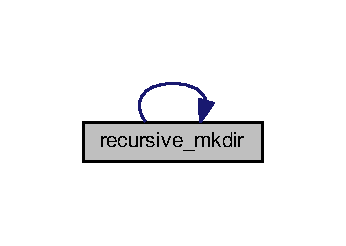
\includegraphics[width=166pt]{Auxiliars_8c_a572fc7e90a3041bc8c17d3f23ad0a78d_cgraph}
\end{center}
\end{figure}


\hypertarget{Auxiliars_8c_a07ed422b9084fb6a2fc2edb155ae590b}{\index{Auxiliars.\-c@{Auxiliars.\-c}!redirect\-\_\-stdout@{redirect\-\_\-stdout}}
\index{redirect\-\_\-stdout@{redirect\-\_\-stdout}!Auxiliars.c@{Auxiliars.\-c}}
\subsubsection[{redirect\-\_\-stdout}]{\setlength{\rightskip}{0pt plus 5cm}void redirect\-\_\-stdout (
\begin{DoxyParamCaption}
\item[{char $\ast$}]{str\-File}
\end{DoxyParamCaption}
)}}\label{Auxiliars_8c_a07ed422b9084fb6a2fc2edb155ae590b}
\hypertarget{Auxiliars_8c_a59689ac62cb991f149d59ff57f678550}{\index{Auxiliars.\-c@{Auxiliars.\-c}!replace@{replace}}
\index{replace@{replace}!Auxiliars.c@{Auxiliars.\-c}}
\subsubsection[{replace}]{\setlength{\rightskip}{0pt plus 5cm}char$\ast$ replace (
\begin{DoxyParamCaption}
\item[{char const $\ast$const}]{original, }
\item[{char const $\ast$const}]{pattern, }
\item[{char const $\ast$const}]{replacement}
\end{DoxyParamCaption}
)}}\label{Auxiliars_8c_a59689ac62cb991f149d59ff57f678550}
\hypertarget{Auxiliars_8c_a6fb95aaf1a67c0dfc9e35416a96e58aa}{\index{Auxiliars.\-c@{Auxiliars.\-c}!replace\-\_\-char@{replace\-\_\-char}}
\index{replace\-\_\-char@{replace\-\_\-char}!Auxiliars.c@{Auxiliars.\-c}}
\subsubsection[{replace\-\_\-char}]{\setlength{\rightskip}{0pt plus 5cm}char$\ast$ replace\-\_\-char (
\begin{DoxyParamCaption}
\item[{const char $\ast$}]{s, }
\item[{char}]{ch, }
\item[{const char $\ast$}]{repl}
\end{DoxyParamCaption}
)}}\label{Auxiliars_8c_a6fb95aaf1a67c0dfc9e35416a96e58aa}
\hypertarget{Auxiliars_8c_af1f1971eb763b91534b6d0037b284193}{\index{Auxiliars.\-c@{Auxiliars.\-c}!save\-Config\-And\-Environment\-Files@{save\-Config\-And\-Environment\-Files}}
\index{save\-Config\-And\-Environment\-Files@{save\-Config\-And\-Environment\-Files}!Auxiliars.c@{Auxiliars.\-c}}
\subsubsection[{save\-Config\-And\-Environment\-Files}]{\setlength{\rightskip}{0pt plus 5cm}void save\-Config\-And\-Environment\-Files (
\begin{DoxyParamCaption}
{}
\end{DoxyParamCaption}
)}}\label{Auxiliars_8c_af1f1971eb763b91534b6d0037b284193}


Here is the call graph for this function\-:\nopagebreak
\begin{figure}[H]
\begin{center}
\leavevmode
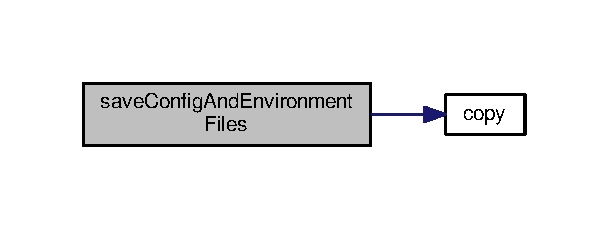
\includegraphics[width=292pt]{Auxiliars_8c_af1f1971eb763b91534b6d0037b284193_cgraph}
\end{center}
\end{figure}


\hypertarget{Auxiliars_8c_ac08052e787477c50ef64b7ab0d7f1424}{\index{Auxiliars.\-c@{Auxiliars.\-c}!show\-Debug\-Options@{show\-Debug\-Options}}
\index{show\-Debug\-Options@{show\-Debug\-Options}!Auxiliars.c@{Auxiliars.\-c}}
\subsubsection[{show\-Debug\-Options}]{\setlength{\rightskip}{0pt plus 5cm}void show\-Debug\-Options (
\begin{DoxyParamCaption}
{}
\end{DoxyParamCaption}
)}}\label{Auxiliars_8c_ac08052e787477c50ef64b7ab0d7f1424}

\hypertarget{Auxiliars_8h}{\section{Auxiliars.\-h File Reference}
\label{Auxiliars_8h}\index{Auxiliars.\-h@{Auxiliars.\-h}}
}
This graph shows which files directly or indirectly include this file\-:\nopagebreak
\begin{figure}[H]
\begin{center}
\leavevmode
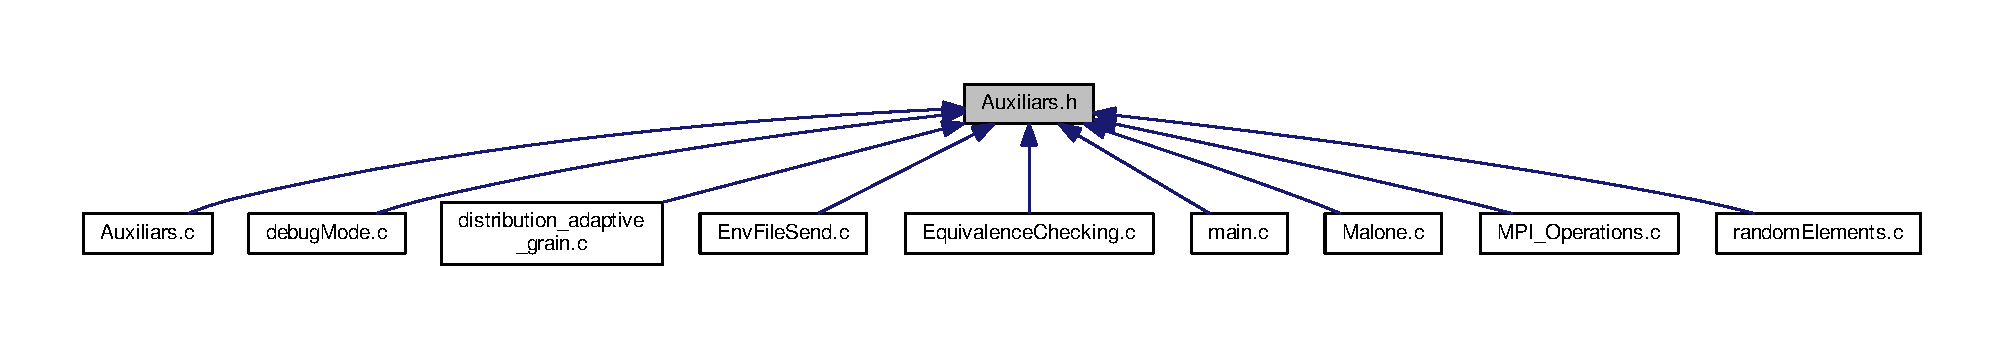
\includegraphics[width=350pt]{Auxiliars_8h__dep__incl}
\end{center}
\end{figure}
\subsection*{Macros}
\begin{DoxyCompactItemize}
\item 
\#define \hyperlink{Auxiliars_8h_a34c026beddb45c2c1cdb60bc793deced}{D\-E\-B\-U\-G\-\_\-\-A\-U\-X}~\hyperlink{Auxiliars_8h_a9fc952cf76aa8896184df882c33ed1c8}{is\-Enabled\-Aux\-Log}()
\item 
\#define \hyperlink{Auxiliars_8h_a11a4f3e4168dc57c71556e5f17ffef0a}{M\-A\-L\-O\-N\-E\-\_\-\-M\-A\-I\-N\-\_\-\-C\-O\-M\-M\-A\-N\-D}~\hyperlink{Auxiliars_8h_af3d2268d78c36203c367ad1fe581743f}{is\-Enabled\-Debug\-Main\-Command\-Log}()
\end{DoxyCompactItemize}
\subsection*{Functions}
\begin{DoxyCompactItemize}
\item 
int \hyperlink{Auxiliars_8h_a5891dfe1066ac082980db1c3eb4c9f2c}{pretty\-Print} (int n\-Index, int n\-Total, int n\-Ant\-Prog)
\item 
int \hyperlink{Auxiliars_8h_ac65810d8fde88b1a003403d3894e070e}{get\-Original\-Time} (\hyperlink{structT__stTestList}{T\-\_\-st\-Test\-List} $\ast$p\-List, int n\-Test)
\item 
int \hyperlink{Auxiliars_8h_aa18130a85476ab3847ee9eb448fc4f03}{check\-Result\-Original} (int n\-Index\-Test, const char $\ast$str\-Result)
\item 
int \hyperlink{Auxiliars_8h_a1676fd50e6015c0f173b606f30b20127}{check\-Test\-Result\-Original} (\hyperlink{structT__stTestInfo}{T\-\_\-st\-Test\-Info} $\ast$p\-Test)
\item 
int \hyperlink{Auxiliars_8h_a36f2832c38f67826aefb581cde8200fb}{test\-Vector} ()
\item 
int \hyperlink{Auxiliars_8h_a438dd8b30a1f8b16fd956363f6909f29}{read\-Test\-Suite} ()
\item 
int \hyperlink{Auxiliars_8h_a83dd3e45bbd9220ce41c2a2785ee2571}{check\-Result} (int n\-Index\-Test, const char $\ast$str\-Result)
\item 
int \hyperlink{Auxiliars_8h_a483eea21188eae7d531a113493aacd6b}{check\-Test\-Result} (\hyperlink{structT__stTestInfo}{T\-\_\-st\-Test\-Info} $\ast$p\-Test)
\item 
void \hyperlink{Auxiliars_8h_a146a12561b1a6fdedea1505ac4434faa}{insert\-Full\-Mutant\-Info} (int n\-Mutant, int n\-Mutant\-State, \hyperlink{structT__stTestList}{T\-\_\-st\-Test\-List} $\ast$p\-List)
\item 
int \hyperlink{Auxiliars_8h_afa2214923ca27bb087ebe0622ba7c152}{insert\-Test\-Result} (int n\-Mutant, int n\-Test, \hyperlink{structT__stTestInfo}{T\-\_\-st\-Test\-Info} $\ast$p\-Test)
\item 
int \hyperlink{Auxiliars_8h_a468c24e305d956cf0bb31debf9ff8a97}{insert\-Test\-Result\-\_\-unsorted} (int n\-Mutant, int n\-Test, \hyperlink{structT__stTestInfo}{T\-\_\-st\-Test\-Info} $\ast$p\-Test)
\item 
void \hyperlink{Auxiliars_8h_a3b80d6dfc602edb25b80149fffe6ea9b}{insert\-Mutant} (\hyperlink{structT__stMutant}{T\-\_\-st\-Mutant} $\ast$p\-Mutant, int n\-Index\-Mutant)
\item 
void \hyperlink{Auxiliars_8h_ae868349a1b9962bef735c645c8af8429}{insert\-Mutant\-Test\-By\-Test} (\hyperlink{structT__stMutant}{T\-\_\-st\-Mutant} $\ast$p\-Mutant, int n\-Index\-Mutant, int n\-Worker\-Source)
\item 
int \hyperlink{Auxiliars_8h_a3ac75c1ea5af10a333cbda886d5b486d}{alloc\-Mutant} (int n\-Index\-Mutant)
\item 
int \hyperlink{Auxiliars_8h_ad977bb957ddd724b9dd590e37d9fe093}{is\-Mutant\-Allocated} (int n\-Index\-Mutant)
\item 
char $\ast$ \hyperlink{Auxiliars_8h_a82109f9207eb5c668dcffd36565eaee7}{build\-Exe\-Line\-\_\-general} (int n\-Index\-Mutant, int n\-Index\-Test, int n\-Original\-Mode)
\item 
char $\ast$ \hyperlink{Auxiliars_8h_a94eb643b244f2e7018d5a205b18cd4dc}{build\-Exe\-Line\-\_\-\-Stand\-Alone} (int n\-Index\-Mutant, int n\-Index\-Test, int n\-Original\-Mode)
\item 
void \hyperlink{Auxiliars_8h_a0021dd07c447d6eecf839803f987b7c9}{add\-Result\-Index} (\hyperlink{structT__stTestList}{T\-\_\-st\-Test\-List} $\ast$p\-Test\-List, int n\-Index, const char $\ast$t, double d\-Time, int n\-Kill)
\item 
void \hyperlink{Auxiliars_8h_a7387501825c9e531f32281f0dcf07e07}{initialize\-Equivalent\-Map} (int n\-Mutants, int n\-Tests)
\item 
void \hyperlink{Auxiliars_8h_aad2abc7509dca3a174711497c2a2bbe4}{initialize\-Execution\-Map} (int n\-Mutants, int n\-Tests)
\item 
void \hyperlink{Auxiliars_8h_a10491c96545ab6d0b126d2ca0db07cc6}{initialize\-\_\-auxiliars} ()
\item 
int \hyperlink{Auxiliars_8h_a6d20a5a58c64584accdeb1a904de9d83}{add\-Result} (\hyperlink{structT__stTestList}{T\-\_\-st\-Test\-List} $\ast$p\-Test\-List, const char $\ast$t, double d\-Time, int n\-Kill)
\item 
\hyperlink{structT__stTestInfo}{T\-\_\-st\-Test\-Info} $\ast$ \hyperlink{Auxiliars_8h_a256f1dad89862377930e90a792b8e37d}{create\-Test} (int n\-Index\-Test, char $\ast$str\-Result, double d\-Time, int n\-Kill)
\item 
char $\ast$ \hyperlink{Auxiliars_8h_a89d711e5c117f1a990a8cf5e5c8630dc}{build\-Exe\-Line} (int n\-Index\-Mutant, int n\-Index\-Test, int n\-Original\-Mode)
\item 
char $\ast$ \hyperlink{Auxiliars_8h_abf20f0d0256aca4acc21a8bcef943aa2}{generate\-Compilation\-Line} (int n\-Index\-Mutant, int n\-Original\-Mode)
\item 
void \hyperlink{Auxiliars_8h_ac08052e787477c50ef64b7ab0d7f1424}{show\-Debug\-Options} ()
\item 
int \hyperlink{Auxiliars_8h_a9fc952cf76aa8896184df882c33ed1c8}{is\-Enabled\-Aux\-Log} ()
\item 
int \hyperlink{Auxiliars_8h_af3d2268d78c36203c367ad1fe581743f}{is\-Enabled\-Debug\-Main\-Command\-Log} ()
\item 
int \hyperlink{Auxiliars_8h_a3201f70287d7dcf94efb84b3629deaf0}{generate\-Res\-Folder} ()
\item 
void \hyperlink{Auxiliars_8h_af1f1971eb763b91534b6d0037b284193}{save\-Config\-And\-Environment\-Files} ()
\item 
\hyperlink{structMutantList}{Mutant\-List} $\ast$ \hyperlink{Auxiliars_8h_af0f8d130a0e61d129d7173fdada44943}{generate\-Clean\-Mutant\-List} (int n\-Mutants)
\item 
void \hyperlink{Auxiliars_8h_a3abc72bb2b5e7aa536901b5c47dd146f}{free\-Mutant\-List} (\hyperlink{structMutantList}{Mutant\-List} $\ast$p\-List)
\item 
long int \hyperlink{Auxiliars_8h_a60ab9fcbd72061289ed7af622754751b}{get\-Tick} ()
\item 
int \hyperlink{Auxiliars_8h_ad524f269a2713fec2f64053c3704503b}{getenv\-\_\-int} (char $\ast$str\-Key)
\item 
char $\ast$ \hyperlink{Auxiliars_8h_a59689ac62cb991f149d59ff57f678550}{replace} (char const $\ast$const original, char const $\ast$const pattern, char const $\ast$const replacement)
\item 
char $\ast$ \hyperlink{Auxiliars_8h_a6fb95aaf1a67c0dfc9e35416a96e58aa}{replace\-\_\-char} (const char $\ast$s, char ch, const char $\ast$repl)
\item 
int \hyperlink{Auxiliars_8h_a928b1da945af8413e422d1749058d33a}{file\-\_\-exist} (char $\ast$filename)
\item 
char $\ast$ \hyperlink{Auxiliars_8h_a312b37675e7e147fb30b0cb53d7d8479}{exec\-Command\-Line} (const char $\ast$fmt,...)
\item 
F\-I\-L\-E $\ast$ \hyperlink{Auxiliars_8h_a60db6d4d611a750ba6e19774ac2bcebb}{fopen\-\_\-mkdir} (char $\ast$path, char $\ast$mode)
\item 
void \hyperlink{Auxiliars_8h_a07ed422b9084fb6a2fc2edb155ae590b}{redirect\-\_\-stdout} (char $\ast$str\-File)
\item 
void \hyperlink{Auxiliars_8h_a572fc7e90a3041bc8c17d3f23ad0a78d}{recursive\-\_\-mkdir} (char $\ast$path)
\item 
void \hyperlink{Auxiliars_8h_a41d4d001d9bf9a77465ed907374e0658}{copy} (char $\ast$source, char $\ast$dest)
\end{DoxyCompactItemize}


\subsection{Macro Definition Documentation}
\hypertarget{Auxiliars_8h_a34c026beddb45c2c1cdb60bc793deced}{\index{Auxiliars.\-h@{Auxiliars.\-h}!D\-E\-B\-U\-G\-\_\-\-A\-U\-X@{D\-E\-B\-U\-G\-\_\-\-A\-U\-X}}
\index{D\-E\-B\-U\-G\-\_\-\-A\-U\-X@{D\-E\-B\-U\-G\-\_\-\-A\-U\-X}!Auxiliars.h@{Auxiliars.\-h}}
\subsubsection[{D\-E\-B\-U\-G\-\_\-\-A\-U\-X}]{\setlength{\rightskip}{0pt plus 5cm}\#define D\-E\-B\-U\-G\-\_\-\-A\-U\-X~{\bf is\-Enabled\-Aux\-Log}()}}\label{Auxiliars_8h_a34c026beddb45c2c1cdb60bc793deced}
\hypertarget{Auxiliars_8h_a11a4f3e4168dc57c71556e5f17ffef0a}{\index{Auxiliars.\-h@{Auxiliars.\-h}!M\-A\-L\-O\-N\-E\-\_\-\-M\-A\-I\-N\-\_\-\-C\-O\-M\-M\-A\-N\-D@{M\-A\-L\-O\-N\-E\-\_\-\-M\-A\-I\-N\-\_\-\-C\-O\-M\-M\-A\-N\-D}}
\index{M\-A\-L\-O\-N\-E\-\_\-\-M\-A\-I\-N\-\_\-\-C\-O\-M\-M\-A\-N\-D@{M\-A\-L\-O\-N\-E\-\_\-\-M\-A\-I\-N\-\_\-\-C\-O\-M\-M\-A\-N\-D}!Auxiliars.h@{Auxiliars.\-h}}
\subsubsection[{M\-A\-L\-O\-N\-E\-\_\-\-M\-A\-I\-N\-\_\-\-C\-O\-M\-M\-A\-N\-D}]{\setlength{\rightskip}{0pt plus 5cm}\#define M\-A\-L\-O\-N\-E\-\_\-\-M\-A\-I\-N\-\_\-\-C\-O\-M\-M\-A\-N\-D~{\bf is\-Enabled\-Debug\-Main\-Command\-Log}()}}\label{Auxiliars_8h_a11a4f3e4168dc57c71556e5f17ffef0a}


\subsection{Function Documentation}
\hypertarget{Auxiliars_8h_a6d20a5a58c64584accdeb1a904de9d83}{\index{Auxiliars.\-h@{Auxiliars.\-h}!add\-Result@{add\-Result}}
\index{add\-Result@{add\-Result}!Auxiliars.h@{Auxiliars.\-h}}
\subsubsection[{add\-Result}]{\setlength{\rightskip}{0pt plus 5cm}int add\-Result (
\begin{DoxyParamCaption}
\item[{{\bf T\-\_\-st\-Test\-List} $\ast$}]{p\-Test\-List, }
\item[{const char $\ast$}]{t, }
\item[{double}]{d\-Time, }
\item[{int}]{n\-Kill}
\end{DoxyParamCaption}
)}}\label{Auxiliars_8h_a6d20a5a58c64584accdeb1a904de9d83}
\hypertarget{Auxiliars_8h_a0021dd07c447d6eecf839803f987b7c9}{\index{Auxiliars.\-h@{Auxiliars.\-h}!add\-Result\-Index@{add\-Result\-Index}}
\index{add\-Result\-Index@{add\-Result\-Index}!Auxiliars.h@{Auxiliars.\-h}}
\subsubsection[{add\-Result\-Index}]{\setlength{\rightskip}{0pt plus 5cm}void add\-Result\-Index (
\begin{DoxyParamCaption}
\item[{{\bf T\-\_\-st\-Test\-List} $\ast$}]{p\-Test\-List, }
\item[{int}]{n\-Index, }
\item[{const char $\ast$}]{t, }
\item[{double}]{d\-Time, }
\item[{int}]{n\-Kill}
\end{DoxyParamCaption}
)}}\label{Auxiliars_8h_a0021dd07c447d6eecf839803f987b7c9}
\hypertarget{Auxiliars_8h_a3ac75c1ea5af10a333cbda886d5b486d}{\index{Auxiliars.\-h@{Auxiliars.\-h}!alloc\-Mutant@{alloc\-Mutant}}
\index{alloc\-Mutant@{alloc\-Mutant}!Auxiliars.h@{Auxiliars.\-h}}
\subsubsection[{alloc\-Mutant}]{\setlength{\rightskip}{0pt plus 5cm}int alloc\-Mutant (
\begin{DoxyParamCaption}
\item[{int}]{n\-Index\-Mutant}
\end{DoxyParamCaption}
)}}\label{Auxiliars_8h_a3ac75c1ea5af10a333cbda886d5b486d}


Here is the call graph for this function\-:\nopagebreak
\begin{figure}[H]
\begin{center}
\leavevmode
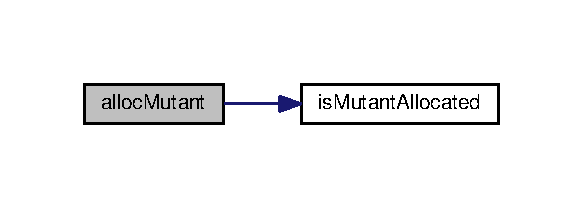
\includegraphics[width=280pt]{Auxiliars_8h_a3ac75c1ea5af10a333cbda886d5b486d_cgraph}
\end{center}
\end{figure}


\hypertarget{Auxiliars_8h_a89d711e5c117f1a990a8cf5e5c8630dc}{\index{Auxiliars.\-h@{Auxiliars.\-h}!build\-Exe\-Line@{build\-Exe\-Line}}
\index{build\-Exe\-Line@{build\-Exe\-Line}!Auxiliars.h@{Auxiliars.\-h}}
\subsubsection[{build\-Exe\-Line}]{\setlength{\rightskip}{0pt plus 5cm}char$\ast$ build\-Exe\-Line (
\begin{DoxyParamCaption}
\item[{int}]{n\-Index\-Mutant, }
\item[{int}]{n\-Index\-Test, }
\item[{int}]{n\-Original\-Mode}
\end{DoxyParamCaption}
)}}\label{Auxiliars_8h_a89d711e5c117f1a990a8cf5e5c8630dc}


Here is the call graph for this function\-:\nopagebreak
\begin{figure}[H]
\begin{center}
\leavevmode
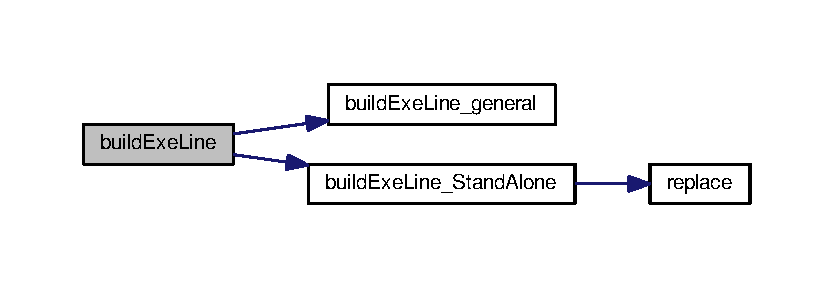
\includegraphics[width=350pt]{Auxiliars_8h_a89d711e5c117f1a990a8cf5e5c8630dc_cgraph}
\end{center}
\end{figure}


\hypertarget{Auxiliars_8h_a82109f9207eb5c668dcffd36565eaee7}{\index{Auxiliars.\-h@{Auxiliars.\-h}!build\-Exe\-Line\-\_\-general@{build\-Exe\-Line\-\_\-general}}
\index{build\-Exe\-Line\-\_\-general@{build\-Exe\-Line\-\_\-general}!Auxiliars.h@{Auxiliars.\-h}}
\subsubsection[{build\-Exe\-Line\-\_\-general}]{\setlength{\rightskip}{0pt plus 5cm}char$\ast$ build\-Exe\-Line\-\_\-general (
\begin{DoxyParamCaption}
\item[{int}]{n\-Index\-Mutant, }
\item[{int}]{n\-Index\-Test, }
\item[{int}]{n\-Original\-Mode}
\end{DoxyParamCaption}
)}}\label{Auxiliars_8h_a82109f9207eb5c668dcffd36565eaee7}
\hypertarget{Auxiliars_8h_a94eb643b244f2e7018d5a205b18cd4dc}{\index{Auxiliars.\-h@{Auxiliars.\-h}!build\-Exe\-Line\-\_\-\-Stand\-Alone@{build\-Exe\-Line\-\_\-\-Stand\-Alone}}
\index{build\-Exe\-Line\-\_\-\-Stand\-Alone@{build\-Exe\-Line\-\_\-\-Stand\-Alone}!Auxiliars.h@{Auxiliars.\-h}}
\subsubsection[{build\-Exe\-Line\-\_\-\-Stand\-Alone}]{\setlength{\rightskip}{0pt plus 5cm}char$\ast$ build\-Exe\-Line\-\_\-\-Stand\-Alone (
\begin{DoxyParamCaption}
\item[{int}]{n\-Index\-Mutant, }
\item[{int}]{n\-Index\-Test, }
\item[{int}]{n\-Original\-Mode}
\end{DoxyParamCaption}
)}}\label{Auxiliars_8h_a94eb643b244f2e7018d5a205b18cd4dc}


Here is the call graph for this function\-:\nopagebreak
\begin{figure}[H]
\begin{center}
\leavevmode
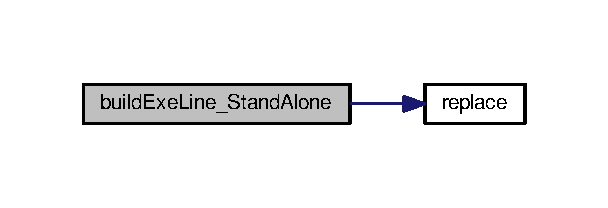
\includegraphics[width=292pt]{Auxiliars_8h_a94eb643b244f2e7018d5a205b18cd4dc_cgraph}
\end{center}
\end{figure}


\hypertarget{Auxiliars_8h_a83dd3e45bbd9220ce41c2a2785ee2571}{\index{Auxiliars.\-h@{Auxiliars.\-h}!check\-Result@{check\-Result}}
\index{check\-Result@{check\-Result}!Auxiliars.h@{Auxiliars.\-h}}
\subsubsection[{check\-Result}]{\setlength{\rightskip}{0pt plus 5cm}int check\-Result (
\begin{DoxyParamCaption}
\item[{int}]{n\-Index\-Test, }
\item[{const char $\ast$}]{str\-Result}
\end{DoxyParamCaption}
)}}\label{Auxiliars_8h_a83dd3e45bbd9220ce41c2a2785ee2571}
\hypertarget{Auxiliars_8h_aa18130a85476ab3847ee9eb448fc4f03}{\index{Auxiliars.\-h@{Auxiliars.\-h}!check\-Result\-Original@{check\-Result\-Original}}
\index{check\-Result\-Original@{check\-Result\-Original}!Auxiliars.h@{Auxiliars.\-h}}
\subsubsection[{check\-Result\-Original}]{\setlength{\rightskip}{0pt plus 5cm}int check\-Result\-Original (
\begin{DoxyParamCaption}
\item[{int}]{n\-Index\-Test, }
\item[{const char $\ast$}]{str\-Result}
\end{DoxyParamCaption}
)}}\label{Auxiliars_8h_aa18130a85476ab3847ee9eb448fc4f03}


Here is the call graph for this function\-:\nopagebreak
\begin{figure}[H]
\begin{center}
\leavevmode
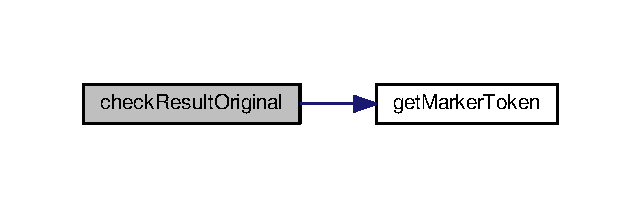
\includegraphics[width=308pt]{Auxiliars_8h_aa18130a85476ab3847ee9eb448fc4f03_cgraph}
\end{center}
\end{figure}


\hypertarget{Auxiliars_8h_a483eea21188eae7d531a113493aacd6b}{\index{Auxiliars.\-h@{Auxiliars.\-h}!check\-Test\-Result@{check\-Test\-Result}}
\index{check\-Test\-Result@{check\-Test\-Result}!Auxiliars.h@{Auxiliars.\-h}}
\subsubsection[{check\-Test\-Result}]{\setlength{\rightskip}{0pt plus 5cm}int check\-Test\-Result (
\begin{DoxyParamCaption}
\item[{{\bf T\-\_\-st\-Test\-Info} $\ast$}]{p\-Test}
\end{DoxyParamCaption}
)}}\label{Auxiliars_8h_a483eea21188eae7d531a113493aacd6b}


Here is the call graph for this function\-:\nopagebreak
\begin{figure}[H]
\begin{center}
\leavevmode
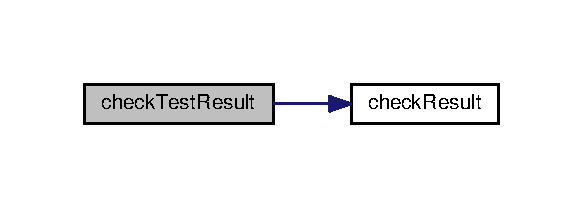
\includegraphics[width=280pt]{Auxiliars_8h_a483eea21188eae7d531a113493aacd6b_cgraph}
\end{center}
\end{figure}


\hypertarget{Auxiliars_8h_a1676fd50e6015c0f173b606f30b20127}{\index{Auxiliars.\-h@{Auxiliars.\-h}!check\-Test\-Result\-Original@{check\-Test\-Result\-Original}}
\index{check\-Test\-Result\-Original@{check\-Test\-Result\-Original}!Auxiliars.h@{Auxiliars.\-h}}
\subsubsection[{check\-Test\-Result\-Original}]{\setlength{\rightskip}{0pt plus 5cm}int check\-Test\-Result\-Original (
\begin{DoxyParamCaption}
\item[{{\bf T\-\_\-st\-Test\-Info} $\ast$}]{p\-Test}
\end{DoxyParamCaption}
)}}\label{Auxiliars_8h_a1676fd50e6015c0f173b606f30b20127}


Here is the call graph for this function\-:\nopagebreak
\begin{figure}[H]
\begin{center}
\leavevmode
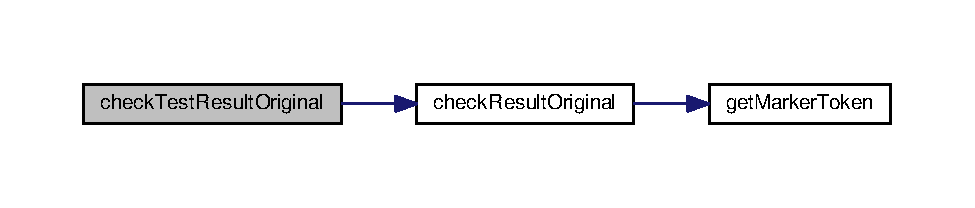
\includegraphics[width=350pt]{Auxiliars_8h_a1676fd50e6015c0f173b606f30b20127_cgraph}
\end{center}
\end{figure}


\hypertarget{Auxiliars_8h_a41d4d001d9bf9a77465ed907374e0658}{\index{Auxiliars.\-h@{Auxiliars.\-h}!copy@{copy}}
\index{copy@{copy}!Auxiliars.h@{Auxiliars.\-h}}
\subsubsection[{copy}]{\setlength{\rightskip}{0pt plus 5cm}void copy (
\begin{DoxyParamCaption}
\item[{char $\ast$}]{source, }
\item[{char $\ast$}]{dest}
\end{DoxyParamCaption}
)}}\label{Auxiliars_8h_a41d4d001d9bf9a77465ed907374e0658}
\hypertarget{Auxiliars_8h_a256f1dad89862377930e90a792b8e37d}{\index{Auxiliars.\-h@{Auxiliars.\-h}!create\-Test@{create\-Test}}
\index{create\-Test@{create\-Test}!Auxiliars.h@{Auxiliars.\-h}}
\subsubsection[{create\-Test}]{\setlength{\rightskip}{0pt plus 5cm}{\bf T\-\_\-st\-Test\-Info}$\ast$ create\-Test (
\begin{DoxyParamCaption}
\item[{int}]{n\-Index\-Test, }
\item[{char $\ast$}]{str\-Result, }
\item[{double}]{d\-Time, }
\item[{int}]{n\-Kill}
\end{DoxyParamCaption}
)}}\label{Auxiliars_8h_a256f1dad89862377930e90a792b8e37d}
\hypertarget{Auxiliars_8h_a312b37675e7e147fb30b0cb53d7d8479}{\index{Auxiliars.\-h@{Auxiliars.\-h}!exec\-Command\-Line@{exec\-Command\-Line}}
\index{exec\-Command\-Line@{exec\-Command\-Line}!Auxiliars.h@{Auxiliars.\-h}}
\subsubsection[{exec\-Command\-Line}]{\setlength{\rightskip}{0pt plus 5cm}char$\ast$ exec\-Command\-Line (
\begin{DoxyParamCaption}
\item[{const char $\ast$}]{fmt, }
\item[{}]{...}
\end{DoxyParamCaption}
)}}\label{Auxiliars_8h_a312b37675e7e147fb30b0cb53d7d8479}
\hypertarget{Auxiliars_8h_a928b1da945af8413e422d1749058d33a}{\index{Auxiliars.\-h@{Auxiliars.\-h}!file\-\_\-exist@{file\-\_\-exist}}
\index{file\-\_\-exist@{file\-\_\-exist}!Auxiliars.h@{Auxiliars.\-h}}
\subsubsection[{file\-\_\-exist}]{\setlength{\rightskip}{0pt plus 5cm}int file\-\_\-exist (
\begin{DoxyParamCaption}
\item[{char $\ast$}]{filename}
\end{DoxyParamCaption}
)}}\label{Auxiliars_8h_a928b1da945af8413e422d1749058d33a}
\hypertarget{Auxiliars_8h_a60db6d4d611a750ba6e19774ac2bcebb}{\index{Auxiliars.\-h@{Auxiliars.\-h}!fopen\-\_\-mkdir@{fopen\-\_\-mkdir}}
\index{fopen\-\_\-mkdir@{fopen\-\_\-mkdir}!Auxiliars.h@{Auxiliars.\-h}}
\subsubsection[{fopen\-\_\-mkdir}]{\setlength{\rightskip}{0pt plus 5cm}F\-I\-L\-E$\ast$ fopen\-\_\-mkdir (
\begin{DoxyParamCaption}
\item[{char $\ast$}]{path, }
\item[{char $\ast$}]{mode}
\end{DoxyParamCaption}
)}}\label{Auxiliars_8h_a60db6d4d611a750ba6e19774ac2bcebb}


Here is the call graph for this function\-:\nopagebreak
\begin{figure}[H]
\begin{center}
\leavevmode
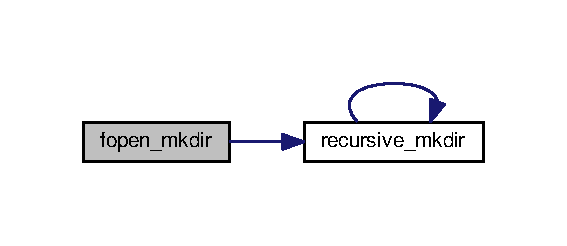
\includegraphics[width=272pt]{Auxiliars_8h_a60db6d4d611a750ba6e19774ac2bcebb_cgraph}
\end{center}
\end{figure}


\hypertarget{Auxiliars_8h_a3abc72bb2b5e7aa536901b5c47dd146f}{\index{Auxiliars.\-h@{Auxiliars.\-h}!free\-Mutant\-List@{free\-Mutant\-List}}
\index{free\-Mutant\-List@{free\-Mutant\-List}!Auxiliars.h@{Auxiliars.\-h}}
\subsubsection[{free\-Mutant\-List}]{\setlength{\rightskip}{0pt plus 5cm}void free\-Mutant\-List (
\begin{DoxyParamCaption}
\item[{{\bf Mutant\-List} $\ast$}]{p\-List}
\end{DoxyParamCaption}
)}}\label{Auxiliars_8h_a3abc72bb2b5e7aa536901b5c47dd146f}
\hypertarget{Auxiliars_8h_af0f8d130a0e61d129d7173fdada44943}{\index{Auxiliars.\-h@{Auxiliars.\-h}!generate\-Clean\-Mutant\-List@{generate\-Clean\-Mutant\-List}}
\index{generate\-Clean\-Mutant\-List@{generate\-Clean\-Mutant\-List}!Auxiliars.h@{Auxiliars.\-h}}
\subsubsection[{generate\-Clean\-Mutant\-List}]{\setlength{\rightskip}{0pt plus 5cm}{\bf Mutant\-List}$\ast$ generate\-Clean\-Mutant\-List (
\begin{DoxyParamCaption}
\item[{int}]{n\-Mutants}
\end{DoxyParamCaption}
)}}\label{Auxiliars_8h_af0f8d130a0e61d129d7173fdada44943}
\hypertarget{Auxiliars_8h_abf20f0d0256aca4acc21a8bcef943aa2}{\index{Auxiliars.\-h@{Auxiliars.\-h}!generate\-Compilation\-Line@{generate\-Compilation\-Line}}
\index{generate\-Compilation\-Line@{generate\-Compilation\-Line}!Auxiliars.h@{Auxiliars.\-h}}
\subsubsection[{generate\-Compilation\-Line}]{\setlength{\rightskip}{0pt plus 5cm}char$\ast$ generate\-Compilation\-Line (
\begin{DoxyParamCaption}
\item[{int}]{n\-Index\-Mutant, }
\item[{int}]{n\-Original\-Mode}
\end{DoxyParamCaption}
)}}\label{Auxiliars_8h_abf20f0d0256aca4acc21a8bcef943aa2}


Here is the call graph for this function\-:\nopagebreak
\begin{figure}[H]
\begin{center}
\leavevmode
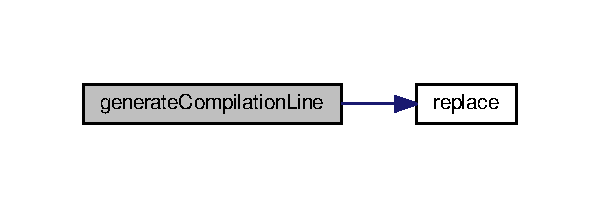
\includegraphics[width=288pt]{Auxiliars_8h_abf20f0d0256aca4acc21a8bcef943aa2_cgraph}
\end{center}
\end{figure}


\hypertarget{Auxiliars_8h_a3201f70287d7dcf94efb84b3629deaf0}{\index{Auxiliars.\-h@{Auxiliars.\-h}!generate\-Res\-Folder@{generate\-Res\-Folder}}
\index{generate\-Res\-Folder@{generate\-Res\-Folder}!Auxiliars.h@{Auxiliars.\-h}}
\subsubsection[{generate\-Res\-Folder}]{\setlength{\rightskip}{0pt plus 5cm}int generate\-Res\-Folder (
\begin{DoxyParamCaption}
{}
\end{DoxyParamCaption}
)}}\label{Auxiliars_8h_a3201f70287d7dcf94efb84b3629deaf0}


Here is the call graph for this function\-:\nopagebreak
\begin{figure}[H]
\begin{center}
\leavevmode
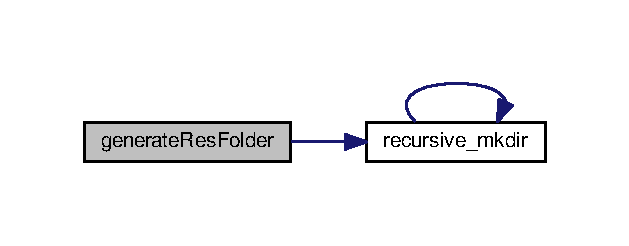
\includegraphics[width=302pt]{Auxiliars_8h_a3201f70287d7dcf94efb84b3629deaf0_cgraph}
\end{center}
\end{figure}


\hypertarget{Auxiliars_8h_ad524f269a2713fec2f64053c3704503b}{\index{Auxiliars.\-h@{Auxiliars.\-h}!getenv\-\_\-int@{getenv\-\_\-int}}
\index{getenv\-\_\-int@{getenv\-\_\-int}!Auxiliars.h@{Auxiliars.\-h}}
\subsubsection[{getenv\-\_\-int}]{\setlength{\rightskip}{0pt plus 5cm}int getenv\-\_\-int (
\begin{DoxyParamCaption}
\item[{char $\ast$}]{str\-Key}
\end{DoxyParamCaption}
)}}\label{Auxiliars_8h_ad524f269a2713fec2f64053c3704503b}
\hypertarget{Auxiliars_8h_ac65810d8fde88b1a003403d3894e070e}{\index{Auxiliars.\-h@{Auxiliars.\-h}!get\-Original\-Time@{get\-Original\-Time}}
\index{get\-Original\-Time@{get\-Original\-Time}!Auxiliars.h@{Auxiliars.\-h}}
\subsubsection[{get\-Original\-Time}]{\setlength{\rightskip}{0pt plus 5cm}int get\-Original\-Time (
\begin{DoxyParamCaption}
\item[{{\bf T\-\_\-st\-Test\-List} $\ast$}]{p\-List, }
\item[{int}]{n\-Test}
\end{DoxyParamCaption}
)}}\label{Auxiliars_8h_ac65810d8fde88b1a003403d3894e070e}
Get the execution time needed to apply the test over the original program 
\begin{DoxyParams}{Parameters}
{\em n\-Test} & \\
\hline
\end{DoxyParams}
\begin{DoxyReturn}{Returns}

\end{DoxyReturn}
\hypertarget{Auxiliars_8h_a60ab9fcbd72061289ed7af622754751b}{\index{Auxiliars.\-h@{Auxiliars.\-h}!get\-Tick@{get\-Tick}}
\index{get\-Tick@{get\-Tick}!Auxiliars.h@{Auxiliars.\-h}}
\subsubsection[{get\-Tick}]{\setlength{\rightskip}{0pt plus 5cm}long int get\-Tick (
\begin{DoxyParamCaption}
{}
\end{DoxyParamCaption}
)}}\label{Auxiliars_8h_a60ab9fcbd72061289ed7af622754751b}
\hypertarget{Auxiliars_8h_a10491c96545ab6d0b126d2ca0db07cc6}{\index{Auxiliars.\-h@{Auxiliars.\-h}!initialize\-\_\-auxiliars@{initialize\-\_\-auxiliars}}
\index{initialize\-\_\-auxiliars@{initialize\-\_\-auxiliars}!Auxiliars.h@{Auxiliars.\-h}}
\subsubsection[{initialize\-\_\-auxiliars}]{\setlength{\rightskip}{0pt plus 5cm}void initialize\-\_\-auxiliars (
\begin{DoxyParamCaption}
{}
\end{DoxyParamCaption}
)}}\label{Auxiliars_8h_a10491c96545ab6d0b126d2ca0db07cc6}
\hypertarget{Auxiliars_8h_a7387501825c9e531f32281f0dcf07e07}{\index{Auxiliars.\-h@{Auxiliars.\-h}!initialize\-Equivalent\-Map@{initialize\-Equivalent\-Map}}
\index{initialize\-Equivalent\-Map@{initialize\-Equivalent\-Map}!Auxiliars.h@{Auxiliars.\-h}}
\subsubsection[{initialize\-Equivalent\-Map}]{\setlength{\rightskip}{0pt plus 5cm}void initialize\-Equivalent\-Map (
\begin{DoxyParamCaption}
\item[{int}]{n\-Mutants, }
\item[{int}]{n\-Tests}
\end{DoxyParamCaption}
)}}\label{Auxiliars_8h_a7387501825c9e531f32281f0dcf07e07}
\hypertarget{Auxiliars_8h_aad2abc7509dca3a174711497c2a2bbe4}{\index{Auxiliars.\-h@{Auxiliars.\-h}!initialize\-Execution\-Map@{initialize\-Execution\-Map}}
\index{initialize\-Execution\-Map@{initialize\-Execution\-Map}!Auxiliars.h@{Auxiliars.\-h}}
\subsubsection[{initialize\-Execution\-Map}]{\setlength{\rightskip}{0pt plus 5cm}void initialize\-Execution\-Map (
\begin{DoxyParamCaption}
\item[{int}]{n\-Mutants, }
\item[{int}]{n\-Tests}
\end{DoxyParamCaption}
)}}\label{Auxiliars_8h_aad2abc7509dca3a174711497c2a2bbe4}
\hypertarget{Auxiliars_8h_a146a12561b1a6fdedea1505ac4434faa}{\index{Auxiliars.\-h@{Auxiliars.\-h}!insert\-Full\-Mutant\-Info@{insert\-Full\-Mutant\-Info}}
\index{insert\-Full\-Mutant\-Info@{insert\-Full\-Mutant\-Info}!Auxiliars.h@{Auxiliars.\-h}}
\subsubsection[{insert\-Full\-Mutant\-Info}]{\setlength{\rightskip}{0pt plus 5cm}void insert\-Full\-Mutant\-Info (
\begin{DoxyParamCaption}
\item[{int}]{n\-Mutant, }
\item[{int}]{n\-Mutant\-State, }
\item[{{\bf T\-\_\-st\-Test\-List} $\ast$}]{p\-List}
\end{DoxyParamCaption}
)}}\label{Auxiliars_8h_a146a12561b1a6fdedea1505ac4434faa}
\hypertarget{Auxiliars_8h_a3b80d6dfc602edb25b80149fffe6ea9b}{\index{Auxiliars.\-h@{Auxiliars.\-h}!insert\-Mutant@{insert\-Mutant}}
\index{insert\-Mutant@{insert\-Mutant}!Auxiliars.h@{Auxiliars.\-h}}
\subsubsection[{insert\-Mutant}]{\setlength{\rightskip}{0pt plus 5cm}void insert\-Mutant (
\begin{DoxyParamCaption}
\item[{{\bf T\-\_\-st\-Mutant} $\ast$}]{p\-Mutant, }
\item[{int}]{n\-Index\-Mutant}
\end{DoxyParamCaption}
)}}\label{Auxiliars_8h_a3b80d6dfc602edb25b80149fffe6ea9b}
\hypertarget{Auxiliars_8h_ae868349a1b9962bef735c645c8af8429}{\index{Auxiliars.\-h@{Auxiliars.\-h}!insert\-Mutant\-Test\-By\-Test@{insert\-Mutant\-Test\-By\-Test}}
\index{insert\-Mutant\-Test\-By\-Test@{insert\-Mutant\-Test\-By\-Test}!Auxiliars.h@{Auxiliars.\-h}}
\subsubsection[{insert\-Mutant\-Test\-By\-Test}]{\setlength{\rightskip}{0pt plus 5cm}void insert\-Mutant\-Test\-By\-Test (
\begin{DoxyParamCaption}
\item[{{\bf T\-\_\-st\-Mutant} $\ast$}]{p\-Mutant, }
\item[{int}]{n\-Index\-Mutant, }
\item[{int}]{n\-Worker\-Source}
\end{DoxyParamCaption}
)}}\label{Auxiliars_8h_ae868349a1b9962bef735c645c8af8429}


Here is the call graph for this function\-:\nopagebreak
\begin{figure}[H]
\begin{center}
\leavevmode
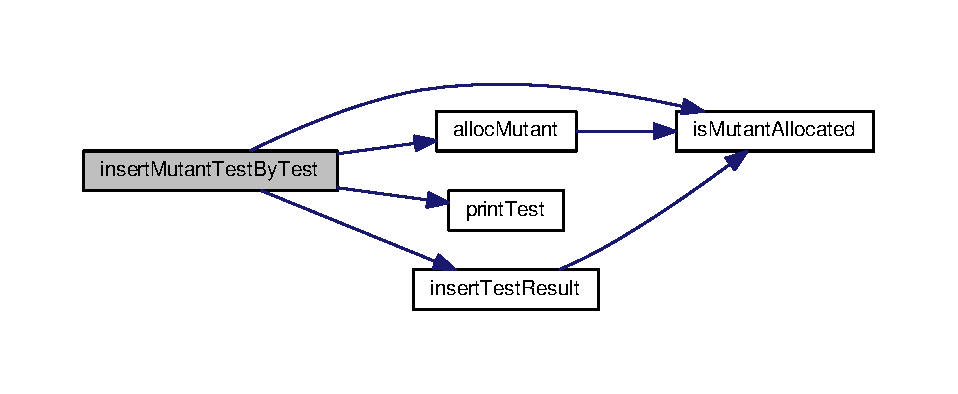
\includegraphics[width=350pt]{Auxiliars_8h_ae868349a1b9962bef735c645c8af8429_cgraph}
\end{center}
\end{figure}


\hypertarget{Auxiliars_8h_afa2214923ca27bb087ebe0622ba7c152}{\index{Auxiliars.\-h@{Auxiliars.\-h}!insert\-Test\-Result@{insert\-Test\-Result}}
\index{insert\-Test\-Result@{insert\-Test\-Result}!Auxiliars.h@{Auxiliars.\-h}}
\subsubsection[{insert\-Test\-Result}]{\setlength{\rightskip}{0pt plus 5cm}int insert\-Test\-Result (
\begin{DoxyParamCaption}
\item[{int}]{n\-Mutant, }
\item[{int}]{n\-Test, }
\item[{{\bf T\-\_\-st\-Test\-Info} $\ast$}]{p\-Test}
\end{DoxyParamCaption}
)}}\label{Auxiliars_8h_afa2214923ca27bb087ebe0622ba7c152}


Here is the call graph for this function\-:\nopagebreak
\begin{figure}[H]
\begin{center}
\leavevmode
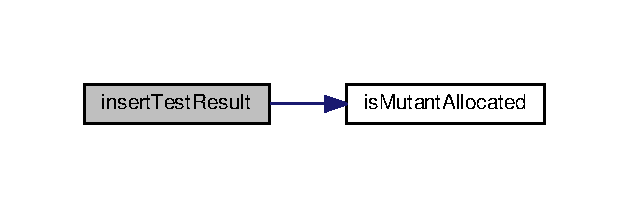
\includegraphics[width=302pt]{Auxiliars_8h_afa2214923ca27bb087ebe0622ba7c152_cgraph}
\end{center}
\end{figure}


\hypertarget{Auxiliars_8h_a468c24e305d956cf0bb31debf9ff8a97}{\index{Auxiliars.\-h@{Auxiliars.\-h}!insert\-Test\-Result\-\_\-unsorted@{insert\-Test\-Result\-\_\-unsorted}}
\index{insert\-Test\-Result\-\_\-unsorted@{insert\-Test\-Result\-\_\-unsorted}!Auxiliars.h@{Auxiliars.\-h}}
\subsubsection[{insert\-Test\-Result\-\_\-unsorted}]{\setlength{\rightskip}{0pt plus 5cm}int insert\-Test\-Result\-\_\-unsorted (
\begin{DoxyParamCaption}
\item[{int}]{n\-Mutant, }
\item[{int}]{n\-Test, }
\item[{{\bf T\-\_\-st\-Test\-Info} $\ast$}]{p\-Test}
\end{DoxyParamCaption}
)}}\label{Auxiliars_8h_a468c24e305d956cf0bb31debf9ff8a97}
This function is designed to insert a test in the first free position in the vector. The main diference with insert\-Result is related with the order. In this case we can have a test vector such \mbox{[}t2,t3,t5\mbox{]} since with insert\-Result we'd have \mbox{[}null,null,t2,t3,null,t5\mbox{]}. We have designed it to achieve a better performance 
\begin{DoxyParams}{Parameters}
{\em n\-Mutant} & Mutant where the test will be inserted \\
\hline
{\em p\-Test} & Test to insert \\
\hline
\end{DoxyParams}
\begin{DoxyReturn}{Returns}
0 if the mutant is not allocated 
\end{DoxyReturn}


Here is the call graph for this function\-:\nopagebreak
\begin{figure}[H]
\begin{center}
\leavevmode
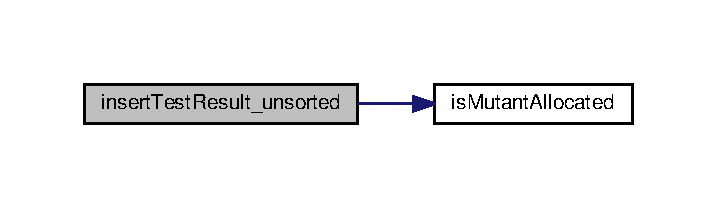
\includegraphics[width=344pt]{Auxiliars_8h_a468c24e305d956cf0bb31debf9ff8a97_cgraph}
\end{center}
\end{figure}


\hypertarget{Auxiliars_8h_a9fc952cf76aa8896184df882c33ed1c8}{\index{Auxiliars.\-h@{Auxiliars.\-h}!is\-Enabled\-Aux\-Log@{is\-Enabled\-Aux\-Log}}
\index{is\-Enabled\-Aux\-Log@{is\-Enabled\-Aux\-Log}!Auxiliars.h@{Auxiliars.\-h}}
\subsubsection[{is\-Enabled\-Aux\-Log}]{\setlength{\rightskip}{0pt plus 5cm}int is\-Enabled\-Aux\-Log (
\begin{DoxyParamCaption}
{}
\end{DoxyParamCaption}
)}}\label{Auxiliars_8h_a9fc952cf76aa8896184df882c33ed1c8}
\hypertarget{Auxiliars_8h_af3d2268d78c36203c367ad1fe581743f}{\index{Auxiliars.\-h@{Auxiliars.\-h}!is\-Enabled\-Debug\-Main\-Command\-Log@{is\-Enabled\-Debug\-Main\-Command\-Log}}
\index{is\-Enabled\-Debug\-Main\-Command\-Log@{is\-Enabled\-Debug\-Main\-Command\-Log}!Auxiliars.h@{Auxiliars.\-h}}
\subsubsection[{is\-Enabled\-Debug\-Main\-Command\-Log}]{\setlength{\rightskip}{0pt plus 5cm}int is\-Enabled\-Debug\-Main\-Command\-Log (
\begin{DoxyParamCaption}
{}
\end{DoxyParamCaption}
)}}\label{Auxiliars_8h_af3d2268d78c36203c367ad1fe581743f}
\hypertarget{Auxiliars_8h_ad977bb957ddd724b9dd590e37d9fe093}{\index{Auxiliars.\-h@{Auxiliars.\-h}!is\-Mutant\-Allocated@{is\-Mutant\-Allocated}}
\index{is\-Mutant\-Allocated@{is\-Mutant\-Allocated}!Auxiliars.h@{Auxiliars.\-h}}
\subsubsection[{is\-Mutant\-Allocated}]{\setlength{\rightskip}{0pt plus 5cm}int is\-Mutant\-Allocated (
\begin{DoxyParamCaption}
\item[{int}]{n\-Index\-Mutant}
\end{DoxyParamCaption}
)}}\label{Auxiliars_8h_ad977bb957ddd724b9dd590e37d9fe093}
\hypertarget{Auxiliars_8h_a5891dfe1066ac082980db1c3eb4c9f2c}{\index{Auxiliars.\-h@{Auxiliars.\-h}!pretty\-Print@{pretty\-Print}}
\index{pretty\-Print@{pretty\-Print}!Auxiliars.h@{Auxiliars.\-h}}
\subsubsection[{pretty\-Print}]{\setlength{\rightskip}{0pt plus 5cm}int pretty\-Print (
\begin{DoxyParamCaption}
\item[{int}]{n\-Index, }
\item[{int}]{n\-Total, }
\item[{int}]{n\-Ant\-Prog}
\end{DoxyParamCaption}
)}}\label{Auxiliars_8h_a5891dfe1066ac082980db1c3eb4c9f2c}
\hypertarget{Auxiliars_8h_a438dd8b30a1f8b16fd956363f6909f29}{\index{Auxiliars.\-h@{Auxiliars.\-h}!read\-Test\-Suite@{read\-Test\-Suite}}
\index{read\-Test\-Suite@{read\-Test\-Suite}!Auxiliars.h@{Auxiliars.\-h}}
\subsubsection[{read\-Test\-Suite}]{\setlength{\rightskip}{0pt plus 5cm}int read\-Test\-Suite (
\begin{DoxyParamCaption}
{}
\end{DoxyParamCaption}
)}}\label{Auxiliars_8h_a438dd8b30a1f8b16fd956363f6909f29}


Here is the call graph for this function\-:\nopagebreak
\begin{figure}[H]
\begin{center}
\leavevmode
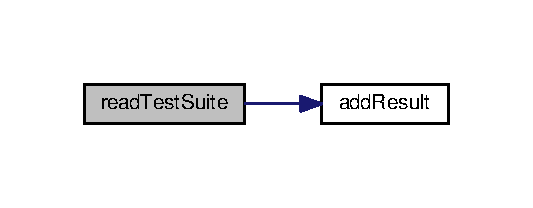
\includegraphics[width=256pt]{Auxiliars_8h_a438dd8b30a1f8b16fd956363f6909f29_cgraph}
\end{center}
\end{figure}


\hypertarget{Auxiliars_8h_a572fc7e90a3041bc8c17d3f23ad0a78d}{\index{Auxiliars.\-h@{Auxiliars.\-h}!recursive\-\_\-mkdir@{recursive\-\_\-mkdir}}
\index{recursive\-\_\-mkdir@{recursive\-\_\-mkdir}!Auxiliars.h@{Auxiliars.\-h}}
\subsubsection[{recursive\-\_\-mkdir}]{\setlength{\rightskip}{0pt plus 5cm}void recursive\-\_\-mkdir (
\begin{DoxyParamCaption}
\item[{char $\ast$}]{path}
\end{DoxyParamCaption}
)}}\label{Auxiliars_8h_a572fc7e90a3041bc8c17d3f23ad0a78d}


Here is the call graph for this function\-:\nopagebreak
\begin{figure}[H]
\begin{center}
\leavevmode
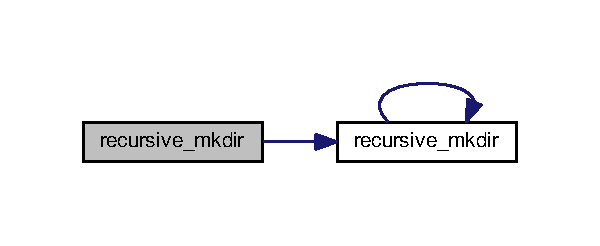
\includegraphics[width=288pt]{Auxiliars_8h_a572fc7e90a3041bc8c17d3f23ad0a78d_cgraph}
\end{center}
\end{figure}


\hypertarget{Auxiliars_8h_a07ed422b9084fb6a2fc2edb155ae590b}{\index{Auxiliars.\-h@{Auxiliars.\-h}!redirect\-\_\-stdout@{redirect\-\_\-stdout}}
\index{redirect\-\_\-stdout@{redirect\-\_\-stdout}!Auxiliars.h@{Auxiliars.\-h}}
\subsubsection[{redirect\-\_\-stdout}]{\setlength{\rightskip}{0pt plus 5cm}void redirect\-\_\-stdout (
\begin{DoxyParamCaption}
\item[{char $\ast$}]{str\-File}
\end{DoxyParamCaption}
)}}\label{Auxiliars_8h_a07ed422b9084fb6a2fc2edb155ae590b}
\hypertarget{Auxiliars_8h_a59689ac62cb991f149d59ff57f678550}{\index{Auxiliars.\-h@{Auxiliars.\-h}!replace@{replace}}
\index{replace@{replace}!Auxiliars.h@{Auxiliars.\-h}}
\subsubsection[{replace}]{\setlength{\rightskip}{0pt plus 5cm}char$\ast$ replace (
\begin{DoxyParamCaption}
\item[{char const $\ast$const}]{original, }
\item[{char const $\ast$const}]{pattern, }
\item[{char const $\ast$const}]{replacement}
\end{DoxyParamCaption}
)}}\label{Auxiliars_8h_a59689ac62cb991f149d59ff57f678550}
\hypertarget{Auxiliars_8h_a6fb95aaf1a67c0dfc9e35416a96e58aa}{\index{Auxiliars.\-h@{Auxiliars.\-h}!replace\-\_\-char@{replace\-\_\-char}}
\index{replace\-\_\-char@{replace\-\_\-char}!Auxiliars.h@{Auxiliars.\-h}}
\subsubsection[{replace\-\_\-char}]{\setlength{\rightskip}{0pt plus 5cm}char$\ast$ replace\-\_\-char (
\begin{DoxyParamCaption}
\item[{const char $\ast$}]{s, }
\item[{char}]{ch, }
\item[{const char $\ast$}]{repl}
\end{DoxyParamCaption}
)}}\label{Auxiliars_8h_a6fb95aaf1a67c0dfc9e35416a96e58aa}
\hypertarget{Auxiliars_8h_af1f1971eb763b91534b6d0037b284193}{\index{Auxiliars.\-h@{Auxiliars.\-h}!save\-Config\-And\-Environment\-Files@{save\-Config\-And\-Environment\-Files}}
\index{save\-Config\-And\-Environment\-Files@{save\-Config\-And\-Environment\-Files}!Auxiliars.h@{Auxiliars.\-h}}
\subsubsection[{save\-Config\-And\-Environment\-Files}]{\setlength{\rightskip}{0pt plus 5cm}void save\-Config\-And\-Environment\-Files (
\begin{DoxyParamCaption}
{}
\end{DoxyParamCaption}
)}}\label{Auxiliars_8h_af1f1971eb763b91534b6d0037b284193}


Here is the call graph for this function\-:\nopagebreak
\begin{figure}[H]
\begin{center}
\leavevmode
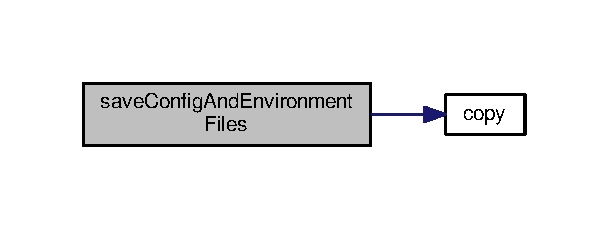
\includegraphics[width=292pt]{Auxiliars_8h_af1f1971eb763b91534b6d0037b284193_cgraph}
\end{center}
\end{figure}


\hypertarget{Auxiliars_8h_ac08052e787477c50ef64b7ab0d7f1424}{\index{Auxiliars.\-h@{Auxiliars.\-h}!show\-Debug\-Options@{show\-Debug\-Options}}
\index{show\-Debug\-Options@{show\-Debug\-Options}!Auxiliars.h@{Auxiliars.\-h}}
\subsubsection[{show\-Debug\-Options}]{\setlength{\rightskip}{0pt plus 5cm}void show\-Debug\-Options (
\begin{DoxyParamCaption}
{}
\end{DoxyParamCaption}
)}}\label{Auxiliars_8h_ac08052e787477c50ef64b7ab0d7f1424}
\hypertarget{Auxiliars_8h_a36f2832c38f67826aefb581cde8200fb}{\index{Auxiliars.\-h@{Auxiliars.\-h}!test\-Vector@{test\-Vector}}
\index{test\-Vector@{test\-Vector}!Auxiliars.h@{Auxiliars.\-h}}
\subsubsection[{test\-Vector}]{\setlength{\rightskip}{0pt plus 5cm}int test\-Vector (
\begin{DoxyParamCaption}
{}
\end{DoxyParamCaption}
)}}\label{Auxiliars_8h_a36f2832c38f67826aefb581cde8200fb}

\hypertarget{configuration_8c}{\section{configuration.\-c File Reference}
\label{configuration_8c}\index{configuration.\-c@{configuration.\-c}}
}
{\ttfamily \#include $<$stdio.\-h$>$}\\*
{\ttfamily \#include $<$stdlib.\-h$>$}\\*
{\ttfamily \#include \char`\"{}configuration.\-h\char`\"{}}\\*
{\ttfamily \#include \char`\"{}Options.\-h\char`\"{}}\\*
Include dependency graph for configuration.\-c\-:\nopagebreak
\begin{figure}[H]
\begin{center}
\leavevmode
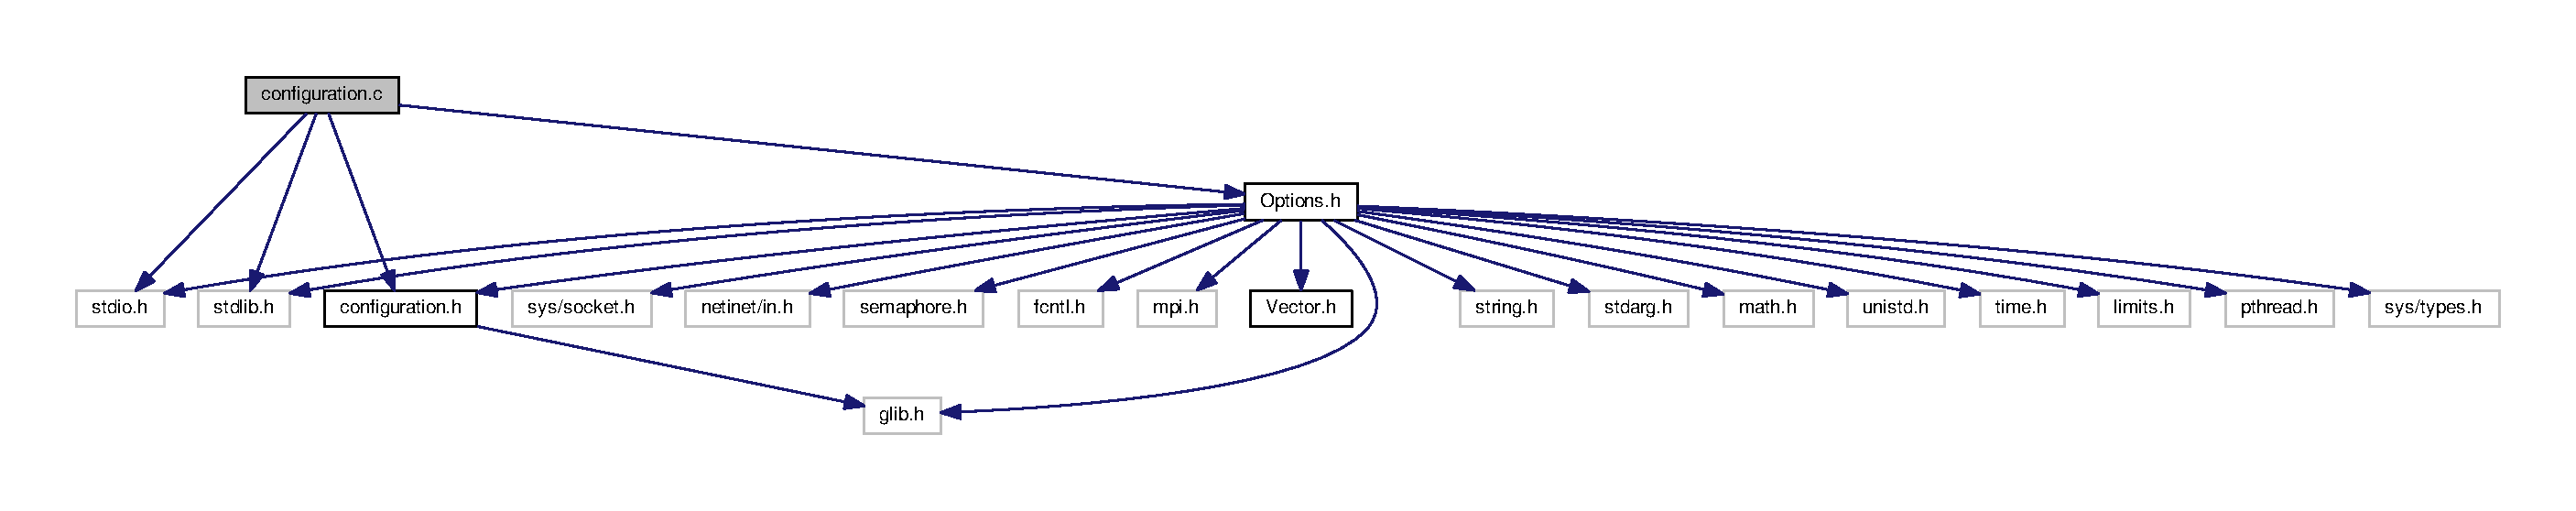
\includegraphics[width=350pt]{configuration_8c__incl}
\end{center}
\end{figure}
\subsection*{Functions}
\begin{DoxyCompactItemize}
\item 
void \hyperlink{configuration_8c_ad5ed6ddd9940c0097cc91774056df1c2}{load\-Config} ()
\item 
\hyperlink{structT__stConfigValues}{T\-\_\-st\-Config\-Values} $\ast$ \hyperlink{configuration_8c_a3cef3589b845d74e6abb41c9d52ada3d}{load\-Config\-From\-Ini} (char $\ast$str\-Path)
\item 
\hyperlink{structT__stIniValues}{T\-\_\-st\-Ini\-Values} $\ast$ \hyperlink{configuration_8c_aa2b23411e3652d16c61db09763bba644}{load\-Environment\-From\-Ini\-File} (char $\ast$str\-Path)
\item 
\hyperlink{structT__stIniValues}{T\-\_\-st\-Ini\-Values} $\ast$ \hyperlink{configuration_8c_a9e8f363ac5cd9dc04603644592421ac4}{load\-Environment\-Keys} (G\-Key\-File $\ast$key\-\_\-file)
\item 
\hyperlink{structT__stIniValues}{T\-\_\-st\-Ini\-Values} $\ast$ \hyperlink{configuration_8c_a63a188784f1a565b87a789e33f3562b3}{load\-Environment\-From\-Ini\-Memory} (const char $\ast$p\-Buffer, int n\-Size)
\item 
int \hyperlink{configuration_8c_ac4b5363f6a34730d07d721a1b3043fc6}{is\-Enabled\-Config\-Log} ()
\end{DoxyCompactItemize}


\subsection{Function Documentation}
\hypertarget{configuration_8c_ac4b5363f6a34730d07d721a1b3043fc6}{\index{configuration.\-c@{configuration.\-c}!is\-Enabled\-Config\-Log@{is\-Enabled\-Config\-Log}}
\index{is\-Enabled\-Config\-Log@{is\-Enabled\-Config\-Log}!configuration.c@{configuration.\-c}}
\subsubsection[{is\-Enabled\-Config\-Log}]{\setlength{\rightskip}{0pt plus 5cm}int is\-Enabled\-Config\-Log (
\begin{DoxyParamCaption}
{}
\end{DoxyParamCaption}
)}}\label{configuration_8c_ac4b5363f6a34730d07d721a1b3043fc6}
\hypertarget{configuration_8c_ad5ed6ddd9940c0097cc91774056df1c2}{\index{configuration.\-c@{configuration.\-c}!load\-Config@{load\-Config}}
\index{load\-Config@{load\-Config}!configuration.c@{configuration.\-c}}
\subsubsection[{load\-Config}]{\setlength{\rightskip}{0pt plus 5cm}void load\-Config (
\begin{DoxyParamCaption}
{}
\end{DoxyParamCaption}
)}}\label{configuration_8c_ad5ed6ddd9940c0097cc91774056df1c2}


Here is the call graph for this function\-:\nopagebreak
\begin{figure}[H]
\begin{center}
\leavevmode
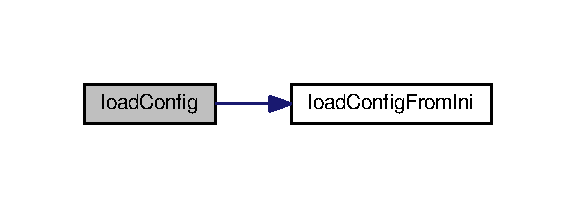
\includegraphics[width=276pt]{configuration_8c_ad5ed6ddd9940c0097cc91774056df1c2_cgraph}
\end{center}
\end{figure}


\hypertarget{configuration_8c_a3cef3589b845d74e6abb41c9d52ada3d}{\index{configuration.\-c@{configuration.\-c}!load\-Config\-From\-Ini@{load\-Config\-From\-Ini}}
\index{load\-Config\-From\-Ini@{load\-Config\-From\-Ini}!configuration.c@{configuration.\-c}}
\subsubsection[{load\-Config\-From\-Ini}]{\setlength{\rightskip}{0pt plus 5cm}{\bf T\-\_\-st\-Config\-Values}$\ast$ load\-Config\-From\-Ini (
\begin{DoxyParamCaption}
\item[{char $\ast$}]{str\-Path}
\end{DoxyParamCaption}
)}}\label{configuration_8c_a3cef3589b845d74e6abb41c9d52ada3d}
\hypertarget{configuration_8c_aa2b23411e3652d16c61db09763bba644}{\index{configuration.\-c@{configuration.\-c}!load\-Environment\-From\-Ini\-File@{load\-Environment\-From\-Ini\-File}}
\index{load\-Environment\-From\-Ini\-File@{load\-Environment\-From\-Ini\-File}!configuration.c@{configuration.\-c}}
\subsubsection[{load\-Environment\-From\-Ini\-File}]{\setlength{\rightskip}{0pt plus 5cm}{\bf T\-\_\-st\-Ini\-Values}$\ast$ load\-Environment\-From\-Ini\-File (
\begin{DoxyParamCaption}
\item[{char $\ast$}]{str\-Path}
\end{DoxyParamCaption}
)}}\label{configuration_8c_aa2b23411e3652d16c61db09763bba644}


Here is the call graph for this function\-:\nopagebreak
\begin{figure}[H]
\begin{center}
\leavevmode
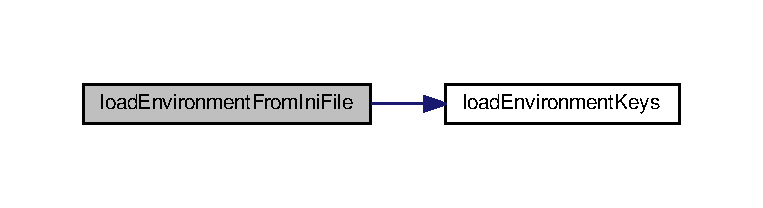
\includegraphics[width=350pt]{configuration_8c_aa2b23411e3652d16c61db09763bba644_cgraph}
\end{center}
\end{figure}


\hypertarget{configuration_8c_a63a188784f1a565b87a789e33f3562b3}{\index{configuration.\-c@{configuration.\-c}!load\-Environment\-From\-Ini\-Memory@{load\-Environment\-From\-Ini\-Memory}}
\index{load\-Environment\-From\-Ini\-Memory@{load\-Environment\-From\-Ini\-Memory}!configuration.c@{configuration.\-c}}
\subsubsection[{load\-Environment\-From\-Ini\-Memory}]{\setlength{\rightskip}{0pt plus 5cm}{\bf T\-\_\-st\-Ini\-Values}$\ast$ load\-Environment\-From\-Ini\-Memory (
\begin{DoxyParamCaption}
\item[{const char $\ast$}]{p\-Buffer, }
\item[{int}]{n\-Size}
\end{DoxyParamCaption}
)}}\label{configuration_8c_a63a188784f1a565b87a789e33f3562b3}


Here is the call graph for this function\-:\nopagebreak
\begin{figure}[H]
\begin{center}
\leavevmode
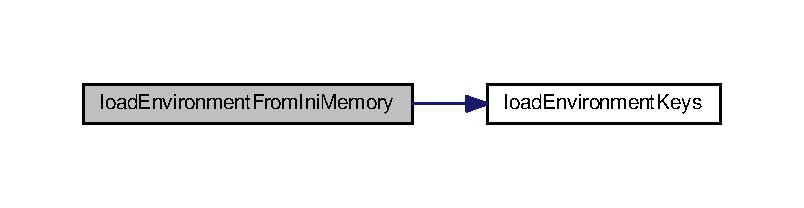
\includegraphics[width=350pt]{configuration_8c_a63a188784f1a565b87a789e33f3562b3_cgraph}
\end{center}
\end{figure}


\hypertarget{configuration_8c_a9e8f363ac5cd9dc04603644592421ac4}{\index{configuration.\-c@{configuration.\-c}!load\-Environment\-Keys@{load\-Environment\-Keys}}
\index{load\-Environment\-Keys@{load\-Environment\-Keys}!configuration.c@{configuration.\-c}}
\subsubsection[{load\-Environment\-Keys}]{\setlength{\rightskip}{0pt plus 5cm}{\bf T\-\_\-st\-Ini\-Values}$\ast$ load\-Environment\-Keys (
\begin{DoxyParamCaption}
\item[{G\-Key\-File $\ast$}]{key\-\_\-file}
\end{DoxyParamCaption}
)}}\label{configuration_8c_a9e8f363ac5cd9dc04603644592421ac4}
Load the .ini file getting the keys associated to the different values that comprises the file. 
\hypertarget{configuration_8h}{\section{configuration.\-h File Reference}
\label{configuration_8h}\index{configuration.\-h@{configuration.\-h}}
}
{\ttfamily \#include $<$glib.\-h$>$}\\*
Include dependency graph for configuration.\-h\-:\nopagebreak
\begin{figure}[H]
\begin{center}
\leavevmode
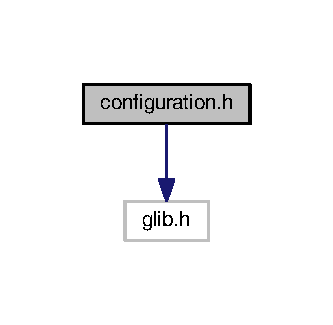
\includegraphics[width=160pt]{configuration_8h__incl}
\end{center}
\end{figure}
This graph shows which files directly or indirectly include this file\-:\nopagebreak
\begin{figure}[H]
\begin{center}
\leavevmode
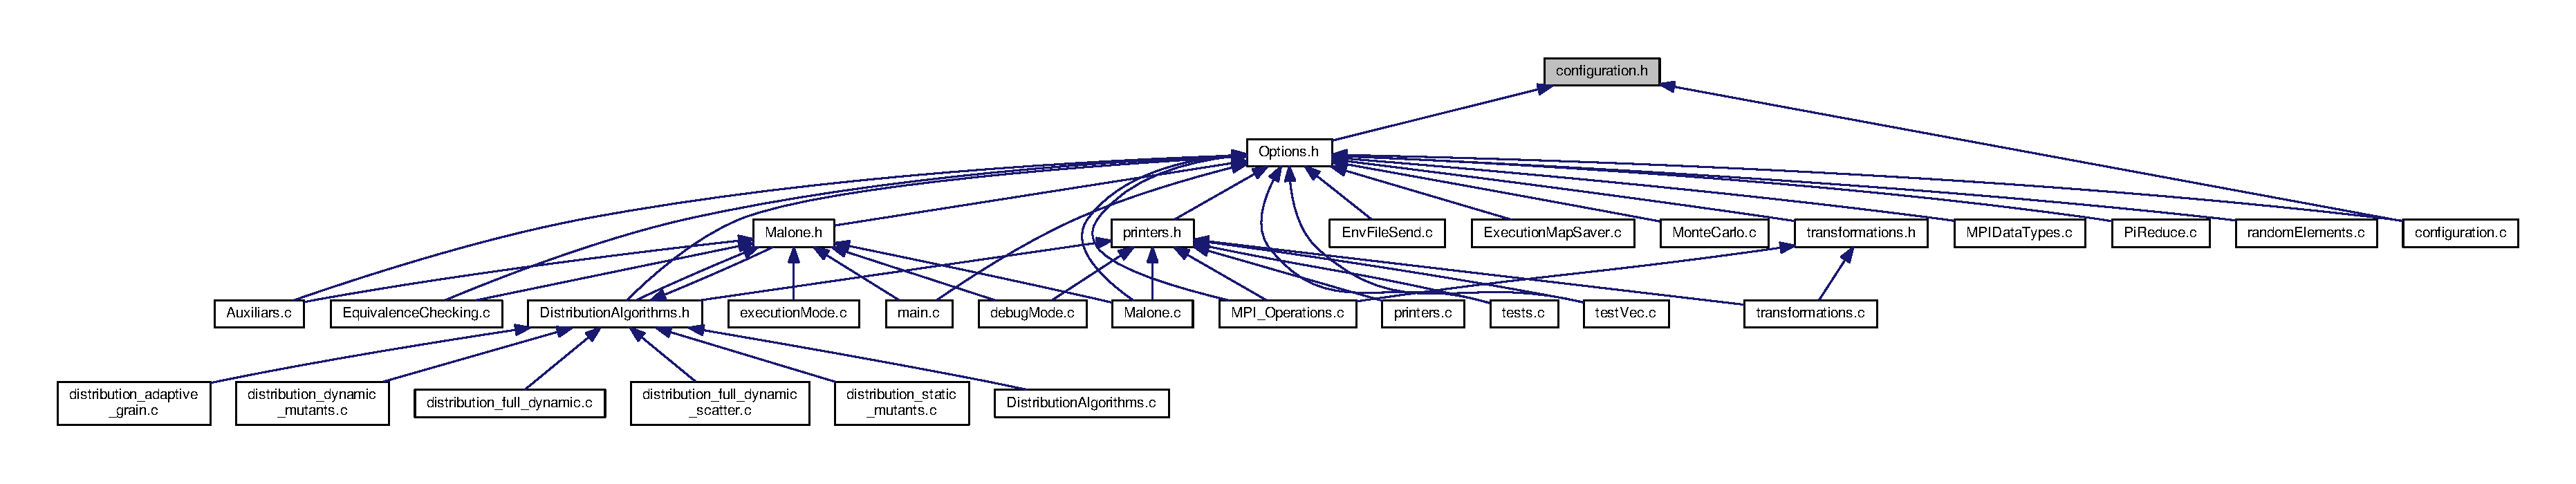
\includegraphics[width=350pt]{configuration_8h__dep__incl}
\end{center}
\end{figure}
\subsection*{Data Structures}
\begin{DoxyCompactItemize}
\item 
struct \hyperlink{structT__stConfigValues}{T\-\_\-st\-Config\-Values}
\item 
struct \hyperlink{structT__stIniValues}{T\-\_\-st\-Ini\-Values}
\end{DoxyCompactItemize}
\subsection*{Macros}
\begin{DoxyCompactItemize}
\item 
\#define \hyperlink{configuration_8h_a5b68e53e9fe03f11c3e476cd598c64c4}{D\-E\-B\-U\-G\-\_\-\-C\-O\-N\-F\-I\-G}~\hyperlink{configuration_8h_ac4b5363f6a34730d07d721a1b3043fc6}{is\-Enabled\-Config\-Log}()
\item 
\#define \hyperlink{configuration_8h_aa8367e84340b96369d3bde17a50fd80f}{P\-A\-T\-H\-\_\-\-E\-N\-V\-\_\-\-D\-I\-R}~\char`\"{}/Environments/\char`\"{}
\item 
\#define \hyperlink{configuration_8h_a06db28c0e7a2cd6eaeb2e870a419e7be}{P\-A\-T\-H\-\_\-\-C\-F\-G\-\_\-\-F\-I\-L\-E}~\char`\"{}Config.\-ini\char`\"{}
\item 
\#define \hyperlink{configuration_8h_a00f0f3788ba424978e6860f020570038}{M\-A\-L\-O\-N\-E\-\_\-\-D\-E\-B\-U\-G\-\_\-\-M\-A\-I\-N\-\_\-\-M\-A\-S\-T\-E\-R}~\char`\"{}M\-A\-L\-O\-N\-E\-\_\-\-D\-E\-B\-U\-G\-\_\-\-M\-A\-I\-N\-\_\-\-M\-A\-S\-T\-E\-R\char`\"{}
\item 
\#define \hyperlink{configuration_8h_ae3a2fa326504f5b30f093b586f463803}{M\-A\-L\-O\-N\-E\-\_\-\-D\-E\-B\-U\-G\-\_\-\-M\-A\-I\-N\-\_\-\-W\-O\-R\-K\-E\-R\-S}~\char`\"{}M\-A\-L\-O\-N\-E\-\_\-\-D\-E\-B\-U\-G\-\_\-\-M\-A\-I\-N\-\_\-\-W\-O\-R\-K\-E\-R\-S\char`\"{}
\item 
\#define \hyperlink{configuration_8h_ab8ce8808383825dc3b02d4297a6c5f3d}{M\-A\-L\-O\-N\-E\-\_\-\-D\-E\-B\-U\-G\-\_\-\-M\-P\-I\-\_\-\-O\-P\-S}~\char`\"{}M\-A\-L\-O\-N\-E\-\_\-\-D\-E\-B\-U\-G\-\_\-\-M\-P\-I\-\_\-\-O\-P\-S\char`\"{}
\item 
\#define \hyperlink{configuration_8h_aa6840d0b7c144329cfab0a875c7a612d}{M\-A\-L\-O\-N\-E\-\_\-\-D\-E\-B\-U\-G\-\_\-\-A\-U\-X}~\char`\"{}M\-A\-L\-O\-N\-E\-\_\-\-D\-E\-B\-U\-G\-\_\-\-A\-U\-X\char`\"{}
\item 
\#define \hyperlink{configuration_8h_a874b5de8771006369f63de1b1a51e78f}{M\-A\-L\-O\-N\-E\-\_\-\-D\-E\-B\-U\-G\-\_\-\-D\-I\-S\-T\-\_\-\-C\-O\-M\-M\-O\-N}~\char`\"{}M\-A\-L\-O\-N\-E\-\_\-\-D\-E\-B\-U\-G\-\_\-\-D\-I\-S\-T\-\_\-\-C\-O\-M\-M\-O\-N\char`\"{}
\item 
\#define \hyperlink{configuration_8h_a2319cbeafffb9f07985a408227aaae5f}{M\-A\-L\-O\-N\-E\-\_\-\-D\-E\-B\-U\-G\-\_\-\-D\-I\-S\-T\-\_\-\-M\-A\-S\-T\-E\-R}~\char`\"{}M\-A\-L\-O\-N\-E\-\_\-\-D\-E\-B\-U\-G\-\_\-\-D\-I\-S\-T\-\_\-\-M\-A\-S\-T\-E\-R\char`\"{}
\item 
\#define \hyperlink{configuration_8h_a1a69f097c78a4845ce5adba7d906685f}{M\-A\-L\-O\-N\-E\-\_\-\-D\-E\-B\-U\-G\-\_\-\-D\-I\-S\-T\-\_\-\-W\-O\-R\-K\-E\-R\-S}~\char`\"{}M\-A\-L\-O\-N\-E\-\_\-\-D\-E\-B\-U\-G\-\_\-\-D\-I\-S\-T\-\_\-\-W\-O\-R\-K\-E\-R\-S\char`\"{}
\item 
\#define \hyperlink{configuration_8h_ad3ff72be9f06cc6df14bc20618563565}{M\-A\-L\-O\-N\-E\-\_\-\-D\-E\-B\-U\-G\-\_\-\-D\-I\-S\-T\-\_\-\-U\-P\-D\-A\-T\-E}~\char`\"{}M\-A\-L\-O\-N\-E\-\_\-\-D\-E\-B\-U\-G\-\_\-\-D\-I\-S\-T\-\_\-\-U\-P\-D\-A\-T\-E\char`\"{}
\item 
\#define \hyperlink{configuration_8h_abc50cc82aceb62f02e195b767eec6814}{M\-A\-L\-O\-N\-E\-\_\-\-D\-E\-B\-U\-G\-\_\-\-T\-R\-A\-N\-S}~\char`\"{}M\-A\-L\-O\-N\-E\-\_\-\-D\-E\-B\-U\-G\-\_\-\-T\-R\-A\-N\-S\char`\"{}
\item 
\#define \hyperlink{configuration_8h_a06490894b7b72427039685493537d4a0}{M\-A\-L\-O\-N\-E\-\_\-\-D\-E\-B\-U\-G\-\_\-\-M\-A\-I\-N\-\_\-\-C\-O\-M\-M\-A\-N\-D}~\char`\"{}M\-A\-L\-O\-N\-E\-\_\-\-D\-E\-B\-U\-G\-\_\-\-M\-A\-I\-N\-\_\-\-C\-O\-M\-M\-A\-N\-D\char`\"{}
\item 
\#define \hyperlink{configuration_8h_a3123f179a859c8d1a1522f237e65e2b9}{M\-A\-L\-O\-N\-E\-\_\-\-D\-E\-B\-U\-G\-\_\-\-P\-R\-I\-N\-T}~\char`\"{}M\-A\-L\-O\-N\-E\-\_\-\-D\-E\-B\-U\-G\-\_\-\-P\-R\-I\-N\-T\char`\"{}
\item 
\#define \hyperlink{configuration_8h_a65de878446091cdf42986ba7d3781c7e}{M\-A\-L\-O\-N\-E\-\_\-\-D\-E\-B\-U\-G\-\_\-\-C\-O\-N\-F\-I\-G}~\char`\"{}M\-A\-L\-O\-N\-E\-\_\-\-D\-E\-B\-U\-G\-\_\-\-C\-O\-N\-F\-I\-G\char`\"{}
\item 
\#define \hyperlink{configuration_8h_a1479256edabe7ff9ae76a4180cc738e1}{M\-A\-L\-O\-N\-E\-\_\-\-R\-E\-D\-I\-R\-E\-C\-T\-I\-O\-N\-\_\-\-F\-I\-L\-E}~\char`\"{}Redirection\-File\char`\"{}
\item 
\#define \hyperlink{configuration_8h_ad11a9c91d1ded1768612f5b6f2648d65}{M\-A\-L\-O\-N\-E\-\_\-\-E\-N\-V\-\_\-\-F\-R\-A\-M\-E\-W\-O\-R\-K\-\_\-\-P\-A\-T\-H}~\char`\"{}Framework\-Path\char`\"{}
\item 
\#define \hyperlink{configuration_8h_a4bbb75c3f7a0a196f3ed52f5041f0d9d}{M\-A\-L\-O\-N\-E\-\_\-\-E\-N\-V\-\_\-\-A\-P\-P\-L\-I\-C\-A\-T\-I\-O\-N\-\_\-\-P\-A\-T\-H}~\char`\"{}Application\-Path\char`\"{}
\item 
\#define \hyperlink{configuration_8h_a3cf92d7b96f9f612f3b2faa6fee25d57}{M\-A\-L\-O\-N\-E\-\_\-\-E\-N\-V\-\_\-\-M\-U\-T\-A\-N\-T\-\_\-\-P\-A\-T\-H}~\char`\"{}Mutant\-Path\char`\"{}
\item 
\#define \hyperlink{configuration_8h_ad321aa4323f36b17c9f40de0845b7f3a}{M\-A\-L\-O\-N\-E\-\_\-\-E\-N\-V\-\_\-\-A\-P\-P\-\_\-\-N\-A\-M\-E}~\char`\"{}Application\-Name\char`\"{}
\item 
\#define \hyperlink{configuration_8h_a32434777c83b0318d8cf0d2ee66182b9}{M\-A\-L\-O\-N\-E\-\_\-\-E\-N\-V\-\_\-\-E\-X\-E\-C\-\_\-\-L\-I\-N\-E\-\_\-\-O\-R\-I\-G\-I\-N\-A\-L}~\char`\"{}Execution\-Line\-Original\char`\"{}
\item 
\#define \hyperlink{configuration_8h_a94763d17ff1e9d4bb06b8f4703cf1000}{M\-A\-L\-O\-N\-E\-\_\-\-E\-N\-V\-\_\-\-E\-X\-E\-C\-\_\-\-L\-I\-N\-E\-\_\-\-M\-U\-T\-A\-N\-T\-S}~\char`\"{}Execution\-Line\-Mutants\char`\"{}
\item 
\#define \hyperlink{configuration_8h_a564c1be8cb4eb171af277c541925e89c}{M\-A\-L\-O\-N\-E\-\_\-\-E\-N\-V\-\_\-\-G\-E\-N\-E\-R\-A\-T\-I\-O\-N\-\_\-\-M\-U\-T\-A\-N\-T\-S\-\_\-\-L\-I\-N\-E}~\char`\"{}Generation\-Line\-Mutants\char`\"{}
\item 
\#define \hyperlink{configuration_8h_a1eccd2e7c9018f3b80e8d52513eb30ce}{M\-A\-L\-O\-N\-E\-\_\-\-E\-N\-V\-\_\-\-T\-O\-T\-A\-L\-\_\-\-T\-E\-S\-T\-S}~\char`\"{}Total\-Tests\char`\"{}
\item 
\#define \hyperlink{configuration_8h_a913a1555a3d3580dacd08d82a54a2525}{M\-A\-L\-O\-N\-E\-\_\-\-E\-N\-V\-\_\-\-T\-O\-T\-A\-L\-\_\-\-M\-U\-T\-A\-N\-T\-S}~\char`\"{}Total\-Mutants\char`\"{}
\item 
\#define \hyperlink{configuration_8h_a55128500befcc406dcc5a21af7cb5037}{M\-A\-L\-O\-N\-E\-\_\-\-E\-N\-V\-\_\-\-S\-T\-A\-R\-T\-I\-N\-G\-\_\-\-M\-U\-T\-A\-N\-T}~\char`\"{}Starting\-Mutant\char`\"{}
\item 
\#define \hyperlink{configuration_8h_a7cdd8dc70f70feafb8046009492debc7}{M\-A\-L\-O\-N\-E\-\_\-\-E\-N\-V\-\_\-\-D\-I\-S\-T\-R\-I\-B\-U\-T\-E\-\_\-\-O\-R\-I\-G\-I\-N\-A\-L}~\char`\"{}Distribute\-Original\char`\"{}
\item 
\#define \hyperlink{configuration_8h_ae7e9d183836e4c26115b951cc7ad0baf}{M\-A\-L\-O\-N\-E\-\_\-\-E\-N\-V\-\_\-\-S\-O\-R\-T\-\_\-\-T\-E\-S\-T\-S\-U\-I\-T\-E}~\char`\"{}Sort\-Test\-Suite\char`\"{}
\item 
\#define \hyperlink{configuration_8h_a5298b69e8e76d8c6b7f4b4ef95e21283}{M\-A\-L\-O\-N\-E\-\_\-\-E\-N\-V\-\_\-\-S\-C\-A\-T\-T\-E\-R\-\_\-\-W\-O\-R\-K\-L\-O\-A\-D}~\char`\"{}Scatter\-Workload\char`\"{}
\item 
\#define \hyperlink{configuration_8h_a6bf083626d5a567d9354bfbfcbd8a8ad}{M\-A\-L\-O\-N\-E\-\_\-\-E\-N\-V\-\_\-\-C\-L\-U\-S\-T\-E\-R\-\_\-\-M\-U\-T\-A\-N\-T\-S}~\char`\"{}Cluster\-Mutants\char`\"{}
\item 
\#define \hyperlink{configuration_8h_a921d7089f0c647360274289a029ca704}{M\-A\-L\-O\-N\-E\-\_\-\-E\-N\-V\-\_\-\-P\-A\-R\-A\-L\-L\-E\-L\-\_\-\-C\-O\-M\-P}~\char`\"{}Parallel\-Compilation\char`\"{}
\item 
\#define \hyperlink{configuration_8h_ae9ba680d127259dfcb629ba0897bee33}{M\-A\-L\-O\-N\-E\-\_\-\-E\-N\-V\-\_\-\-M\-U\-L\-T\-\_\-\-C\-O\-O\-R\-D\-I\-N\-A\-T\-O\-R\-S}~\char`\"{}Multiple\-Coordinators\char`\"{}
\item 
\#define \hyperlink{configuration_8h_a6ebe24733ba86a2f50e19be77ac25b82}{M\-A\-L\-O\-N\-E\-\_\-\-E\-N\-V\-\_\-\-S\-T\-A\-N\-D\-A\-L\-O\-N\-E}~\char`\"{}Standalone\char`\"{}
\item 
\#define \hyperlink{configuration_8h_a73c14eb9b5a4ebc8219d88ac3b523fd3}{M\-A\-L\-O\-N\-E\-\_\-\-E\-N\-V\-\_\-\-T\-E\-S\-T\-S\-U\-I\-T\-E\-\_\-\-F\-I\-L\-E}~\char`\"{}Test\-Suite\-File\char`\"{}
\item 
\#define \hyperlink{configuration_8h_abce905de71559bac9dfae6cf98cee025}{M\-A\-L\-O\-N\-E\-\_\-\-E\-N\-V\-\_\-\-M\-A\-X\-\_\-\-O\-R\-I\-G\-I\-N\-A\-L\-\_\-\-T\-I\-M\-E\-O\-U\-T}~\char`\"{}M\-A\-L\-O\-N\-E\-\_\-\-M\-A\-X\-\_\-\-O\-R\-I\-G\-I\-N\-A\-L\-\_\-\-T\-I\-M\-E\-O\-U\-T\char`\"{}
\item 
\#define \hyperlink{configuration_8h_a1da16971bf037b5327f4f8792231ae64}{M\-A\-L\-O\-N\-E\-\_\-\-E\-N\-V\-\_\-\-M\-A\-X\-\_\-\-M\-U\-T\-A\-N\-T\-S\-\_\-\-T\-I\-M\-E\-O\-U\-T\-\_\-\-F\-A\-C\-T\-O\-R}~\char`\"{}M\-A\-L\-O\-N\-E\-\_\-\-M\-A\-X\-\_\-\-M\-U\-T\-A\-N\-T\-S\-\_\-\-T\-I\-M\-E\-O\-U\-T\-\_\-\-F\-A\-C\-T\-O\-R\char`\"{}
\item 
\#define \hyperlink{configuration_8h_a5f6a8f7d4810a48c4d346861fda3d245}{M\-A\-L\-O\-N\-E\-\_\-\-E\-N\-V\-\_\-\-M\-A\-X\-\_\-\-M\-U\-T\-A\-N\-T\-S\-\_\-\-M\-I\-N\-I\-M\-U\-M\-\_\-\-T\-I\-M\-E}~\char`\"{}M\-A\-L\-O\-N\-E\-\_\-\-M\-A\-X\-\_\-\-M\-U\-T\-A\-N\-T\-S\-\_\-\-M\-I\-N\-I\-M\-U\-M\-\_\-\-T\-I\-M\-E\char`\"{}
\item 
\#define \hyperlink{configuration_8h_a2c01110eef5f2994a1d64444267b1120}{M\-A\-L\-O\-N\-E\-\_\-\-E\-N\-V\-\_\-\-M\-A\-R\-K\-E\-R\-\_\-\-T\-O\-K\-E\-N}~\char`\"{}Marker\-Token\char`\"{}
\item 
\#define \hyperlink{configuration_8h_a3e98dbbe1b47b5e63c65a84c916e8723}{M\-A\-L\-O\-N\-E\-\_\-\-E\-N\-V\-\_\-\-M\-U\-T\-A\-N\-T\-\_\-\-G\-E\-N\-E\-R\-A\-T\-I\-O\-N\-\_\-\-E\-N\-A\-B\-L\-E\-D}~\char`\"{}Mutant\-Generation\-Enabled\char`\"{}
\item 
\#define \hyperlink{configuration_8h_add42512594f345fe75463595d73dd410}{M\-A\-L\-O\-N\-E\-\_\-\-E\-N\-V\-\_\-\-C\-O\-M\-P\-I\-L\-A\-T\-I\-O\-N\-\_\-\-L\-I\-N\-E\-\_\-\-O\-R\-I\-G\-I\-N\-A\-L}~\char`\"{}Compilation\-Line\-Original\char`\"{}
\item 
\#define \hyperlink{configuration_8h_a21f9f8efd2c04e55baed91a24f0dec96}{M\-A\-L\-O\-N\-E\-\_\-\-E\-N\-V\-\_\-\-C\-O\-M\-P\-I\-L\-A\-T\-I\-O\-N\-\_\-\-W\-I\-T\-H\-\_\-\-S\-C\-R\-I\-P\-T}~\char`\"{}Compilation\-With\-Script\char`\"{}
\item 
\#define \hyperlink{configuration_8h_a9ae2392ce6a5500a89d582e08589443b}{M\-A\-L\-O\-N\-E\-\_\-\-E\-N\-V\-\_\-\-C\-O\-M\-P\-I\-L\-A\-T\-I\-O\-N\-\_\-\-L\-I\-N\-E\-\_\-\-M\-U\-T\-A\-N\-T\-S}~\char`\"{}Compilation\-Line\-Mutants\char`\"{}
\item 
\#define \hyperlink{configuration_8h_a8dd14c9b29f73f5b6d6010ad44aa4341}{M\-A\-L\-O\-N\-E\-\_\-\-E\-N\-V\-\_\-\-C\-O\-M\-P\-I\-L\-A\-T\-I\-O\-N\-\_\-\-E\-N\-A\-B\-L\-E\-D}~\char`\"{}Compilation\-Enabled\char`\"{}
\item 
\#define \hyperlink{configuration_8h_a3761da717d8550ca212028f15b759422}{M\-A\-L\-O\-N\-E\-\_\-\-E\-N\-V\-\_\-\-C\-O\-M\-P\-I\-L\-A\-T\-I\-O\-N\-\_\-\-N\-U\-M\-\_\-\-W\-O\-R\-K\-E\-R\-S}~\char`\"{}Compilation\-Num\-Workers\char`\"{}
\item 
\#define \hyperlink{configuration_8h_a9f016ae6ff36410dc84d1c01489dc137}{M\-A\-L\-O\-N\-E\-\_\-\-E\-N\-V\-\_\-\-C\-O\-M\-P\-I\-L\-A\-T\-I\-O\-N\-\_\-\-S\-C\-R\-I\-P\-T}~\char`\"{}Compilation\-Script\char`\"{}
\end{DoxyCompactItemize}
\subsection*{Functions}
\begin{DoxyCompactItemize}
\item 
void \hyperlink{configuration_8h_ad5ed6ddd9940c0097cc91774056df1c2}{load\-Config} ()
\item 
int \hyperlink{configuration_8h_ac4b5363f6a34730d07d721a1b3043fc6}{is\-Enabled\-Config\-Log} ()
\item 
\hyperlink{structT__stConfigValues}{T\-\_\-st\-Config\-Values} $\ast$ \hyperlink{configuration_8h_a3cef3589b845d74e6abb41c9d52ada3d}{load\-Config\-From\-Ini} (char $\ast$str\-Path)
\item 
\hyperlink{structT__stIniValues}{T\-\_\-st\-Ini\-Values} $\ast$ \hyperlink{configuration_8h_a63a188784f1a565b87a789e33f3562b3}{load\-Environment\-From\-Ini\-Memory} (const char $\ast$p\-Buffer, int n\-Size)
\item 
\hyperlink{structT__stIniValues}{T\-\_\-st\-Ini\-Values} $\ast$ \hyperlink{configuration_8h_aa2b23411e3652d16c61db09763bba644}{load\-Environment\-From\-Ini\-File} (char $\ast$str\-Path)
\item 
\hyperlink{structT__stIniValues}{T\-\_\-st\-Ini\-Values} $\ast$ \hyperlink{configuration_8h_a9e8f363ac5cd9dc04603644592421ac4}{load\-Environment\-Keys} (G\-Key\-File $\ast$key\-\_\-file)
\end{DoxyCompactItemize}


\subsection{Macro Definition Documentation}
\hypertarget{configuration_8h_a5b68e53e9fe03f11c3e476cd598c64c4}{\index{configuration.\-h@{configuration.\-h}!D\-E\-B\-U\-G\-\_\-\-C\-O\-N\-F\-I\-G@{D\-E\-B\-U\-G\-\_\-\-C\-O\-N\-F\-I\-G}}
\index{D\-E\-B\-U\-G\-\_\-\-C\-O\-N\-F\-I\-G@{D\-E\-B\-U\-G\-\_\-\-C\-O\-N\-F\-I\-G}!configuration.h@{configuration.\-h}}
\subsubsection[{D\-E\-B\-U\-G\-\_\-\-C\-O\-N\-F\-I\-G}]{\setlength{\rightskip}{0pt plus 5cm}\#define D\-E\-B\-U\-G\-\_\-\-C\-O\-N\-F\-I\-G~{\bf is\-Enabled\-Config\-Log}()}}\label{configuration_8h_a5b68e53e9fe03f11c3e476cd598c64c4}
\hypertarget{configuration_8h_aa6840d0b7c144329cfab0a875c7a612d}{\index{configuration.\-h@{configuration.\-h}!M\-A\-L\-O\-N\-E\-\_\-\-D\-E\-B\-U\-G\-\_\-\-A\-U\-X@{M\-A\-L\-O\-N\-E\-\_\-\-D\-E\-B\-U\-G\-\_\-\-A\-U\-X}}
\index{M\-A\-L\-O\-N\-E\-\_\-\-D\-E\-B\-U\-G\-\_\-\-A\-U\-X@{M\-A\-L\-O\-N\-E\-\_\-\-D\-E\-B\-U\-G\-\_\-\-A\-U\-X}!configuration.h@{configuration.\-h}}
\subsubsection[{M\-A\-L\-O\-N\-E\-\_\-\-D\-E\-B\-U\-G\-\_\-\-A\-U\-X}]{\setlength{\rightskip}{0pt plus 5cm}\#define M\-A\-L\-O\-N\-E\-\_\-\-D\-E\-B\-U\-G\-\_\-\-A\-U\-X~\char`\"{}M\-A\-L\-O\-N\-E\-\_\-\-D\-E\-B\-U\-G\-\_\-\-A\-U\-X\char`\"{}}}\label{configuration_8h_aa6840d0b7c144329cfab0a875c7a612d}
\hypertarget{configuration_8h_a65de878446091cdf42986ba7d3781c7e}{\index{configuration.\-h@{configuration.\-h}!M\-A\-L\-O\-N\-E\-\_\-\-D\-E\-B\-U\-G\-\_\-\-C\-O\-N\-F\-I\-G@{M\-A\-L\-O\-N\-E\-\_\-\-D\-E\-B\-U\-G\-\_\-\-C\-O\-N\-F\-I\-G}}
\index{M\-A\-L\-O\-N\-E\-\_\-\-D\-E\-B\-U\-G\-\_\-\-C\-O\-N\-F\-I\-G@{M\-A\-L\-O\-N\-E\-\_\-\-D\-E\-B\-U\-G\-\_\-\-C\-O\-N\-F\-I\-G}!configuration.h@{configuration.\-h}}
\subsubsection[{M\-A\-L\-O\-N\-E\-\_\-\-D\-E\-B\-U\-G\-\_\-\-C\-O\-N\-F\-I\-G}]{\setlength{\rightskip}{0pt plus 5cm}\#define M\-A\-L\-O\-N\-E\-\_\-\-D\-E\-B\-U\-G\-\_\-\-C\-O\-N\-F\-I\-G~\char`\"{}M\-A\-L\-O\-N\-E\-\_\-\-D\-E\-B\-U\-G\-\_\-\-C\-O\-N\-F\-I\-G\char`\"{}}}\label{configuration_8h_a65de878446091cdf42986ba7d3781c7e}
\hypertarget{configuration_8h_a874b5de8771006369f63de1b1a51e78f}{\index{configuration.\-h@{configuration.\-h}!M\-A\-L\-O\-N\-E\-\_\-\-D\-E\-B\-U\-G\-\_\-\-D\-I\-S\-T\-\_\-\-C\-O\-M\-M\-O\-N@{M\-A\-L\-O\-N\-E\-\_\-\-D\-E\-B\-U\-G\-\_\-\-D\-I\-S\-T\-\_\-\-C\-O\-M\-M\-O\-N}}
\index{M\-A\-L\-O\-N\-E\-\_\-\-D\-E\-B\-U\-G\-\_\-\-D\-I\-S\-T\-\_\-\-C\-O\-M\-M\-O\-N@{M\-A\-L\-O\-N\-E\-\_\-\-D\-E\-B\-U\-G\-\_\-\-D\-I\-S\-T\-\_\-\-C\-O\-M\-M\-O\-N}!configuration.h@{configuration.\-h}}
\subsubsection[{M\-A\-L\-O\-N\-E\-\_\-\-D\-E\-B\-U\-G\-\_\-\-D\-I\-S\-T\-\_\-\-C\-O\-M\-M\-O\-N}]{\setlength{\rightskip}{0pt plus 5cm}\#define M\-A\-L\-O\-N\-E\-\_\-\-D\-E\-B\-U\-G\-\_\-\-D\-I\-S\-T\-\_\-\-C\-O\-M\-M\-O\-N~\char`\"{}M\-A\-L\-O\-N\-E\-\_\-\-D\-E\-B\-U\-G\-\_\-\-D\-I\-S\-T\-\_\-\-C\-O\-M\-M\-O\-N\char`\"{}}}\label{configuration_8h_a874b5de8771006369f63de1b1a51e78f}
\hypertarget{configuration_8h_a2319cbeafffb9f07985a408227aaae5f}{\index{configuration.\-h@{configuration.\-h}!M\-A\-L\-O\-N\-E\-\_\-\-D\-E\-B\-U\-G\-\_\-\-D\-I\-S\-T\-\_\-\-M\-A\-S\-T\-E\-R@{M\-A\-L\-O\-N\-E\-\_\-\-D\-E\-B\-U\-G\-\_\-\-D\-I\-S\-T\-\_\-\-M\-A\-S\-T\-E\-R}}
\index{M\-A\-L\-O\-N\-E\-\_\-\-D\-E\-B\-U\-G\-\_\-\-D\-I\-S\-T\-\_\-\-M\-A\-S\-T\-E\-R@{M\-A\-L\-O\-N\-E\-\_\-\-D\-E\-B\-U\-G\-\_\-\-D\-I\-S\-T\-\_\-\-M\-A\-S\-T\-E\-R}!configuration.h@{configuration.\-h}}
\subsubsection[{M\-A\-L\-O\-N\-E\-\_\-\-D\-E\-B\-U\-G\-\_\-\-D\-I\-S\-T\-\_\-\-M\-A\-S\-T\-E\-R}]{\setlength{\rightskip}{0pt plus 5cm}\#define M\-A\-L\-O\-N\-E\-\_\-\-D\-E\-B\-U\-G\-\_\-\-D\-I\-S\-T\-\_\-\-M\-A\-S\-T\-E\-R~\char`\"{}M\-A\-L\-O\-N\-E\-\_\-\-D\-E\-B\-U\-G\-\_\-\-D\-I\-S\-T\-\_\-\-M\-A\-S\-T\-E\-R\char`\"{}}}\label{configuration_8h_a2319cbeafffb9f07985a408227aaae5f}
\hypertarget{configuration_8h_ad3ff72be9f06cc6df14bc20618563565}{\index{configuration.\-h@{configuration.\-h}!M\-A\-L\-O\-N\-E\-\_\-\-D\-E\-B\-U\-G\-\_\-\-D\-I\-S\-T\-\_\-\-U\-P\-D\-A\-T\-E@{M\-A\-L\-O\-N\-E\-\_\-\-D\-E\-B\-U\-G\-\_\-\-D\-I\-S\-T\-\_\-\-U\-P\-D\-A\-T\-E}}
\index{M\-A\-L\-O\-N\-E\-\_\-\-D\-E\-B\-U\-G\-\_\-\-D\-I\-S\-T\-\_\-\-U\-P\-D\-A\-T\-E@{M\-A\-L\-O\-N\-E\-\_\-\-D\-E\-B\-U\-G\-\_\-\-D\-I\-S\-T\-\_\-\-U\-P\-D\-A\-T\-E}!configuration.h@{configuration.\-h}}
\subsubsection[{M\-A\-L\-O\-N\-E\-\_\-\-D\-E\-B\-U\-G\-\_\-\-D\-I\-S\-T\-\_\-\-U\-P\-D\-A\-T\-E}]{\setlength{\rightskip}{0pt plus 5cm}\#define M\-A\-L\-O\-N\-E\-\_\-\-D\-E\-B\-U\-G\-\_\-\-D\-I\-S\-T\-\_\-\-U\-P\-D\-A\-T\-E~\char`\"{}M\-A\-L\-O\-N\-E\-\_\-\-D\-E\-B\-U\-G\-\_\-\-D\-I\-S\-T\-\_\-\-U\-P\-D\-A\-T\-E\char`\"{}}}\label{configuration_8h_ad3ff72be9f06cc6df14bc20618563565}
\hypertarget{configuration_8h_a1a69f097c78a4845ce5adba7d906685f}{\index{configuration.\-h@{configuration.\-h}!M\-A\-L\-O\-N\-E\-\_\-\-D\-E\-B\-U\-G\-\_\-\-D\-I\-S\-T\-\_\-\-W\-O\-R\-K\-E\-R\-S@{M\-A\-L\-O\-N\-E\-\_\-\-D\-E\-B\-U\-G\-\_\-\-D\-I\-S\-T\-\_\-\-W\-O\-R\-K\-E\-R\-S}}
\index{M\-A\-L\-O\-N\-E\-\_\-\-D\-E\-B\-U\-G\-\_\-\-D\-I\-S\-T\-\_\-\-W\-O\-R\-K\-E\-R\-S@{M\-A\-L\-O\-N\-E\-\_\-\-D\-E\-B\-U\-G\-\_\-\-D\-I\-S\-T\-\_\-\-W\-O\-R\-K\-E\-R\-S}!configuration.h@{configuration.\-h}}
\subsubsection[{M\-A\-L\-O\-N\-E\-\_\-\-D\-E\-B\-U\-G\-\_\-\-D\-I\-S\-T\-\_\-\-W\-O\-R\-K\-E\-R\-S}]{\setlength{\rightskip}{0pt plus 5cm}\#define M\-A\-L\-O\-N\-E\-\_\-\-D\-E\-B\-U\-G\-\_\-\-D\-I\-S\-T\-\_\-\-W\-O\-R\-K\-E\-R\-S~\char`\"{}M\-A\-L\-O\-N\-E\-\_\-\-D\-E\-B\-U\-G\-\_\-\-D\-I\-S\-T\-\_\-\-W\-O\-R\-K\-E\-R\-S\char`\"{}}}\label{configuration_8h_a1a69f097c78a4845ce5adba7d906685f}
\hypertarget{configuration_8h_a06490894b7b72427039685493537d4a0}{\index{configuration.\-h@{configuration.\-h}!M\-A\-L\-O\-N\-E\-\_\-\-D\-E\-B\-U\-G\-\_\-\-M\-A\-I\-N\-\_\-\-C\-O\-M\-M\-A\-N\-D@{M\-A\-L\-O\-N\-E\-\_\-\-D\-E\-B\-U\-G\-\_\-\-M\-A\-I\-N\-\_\-\-C\-O\-M\-M\-A\-N\-D}}
\index{M\-A\-L\-O\-N\-E\-\_\-\-D\-E\-B\-U\-G\-\_\-\-M\-A\-I\-N\-\_\-\-C\-O\-M\-M\-A\-N\-D@{M\-A\-L\-O\-N\-E\-\_\-\-D\-E\-B\-U\-G\-\_\-\-M\-A\-I\-N\-\_\-\-C\-O\-M\-M\-A\-N\-D}!configuration.h@{configuration.\-h}}
\subsubsection[{M\-A\-L\-O\-N\-E\-\_\-\-D\-E\-B\-U\-G\-\_\-\-M\-A\-I\-N\-\_\-\-C\-O\-M\-M\-A\-N\-D}]{\setlength{\rightskip}{0pt plus 5cm}\#define M\-A\-L\-O\-N\-E\-\_\-\-D\-E\-B\-U\-G\-\_\-\-M\-A\-I\-N\-\_\-\-C\-O\-M\-M\-A\-N\-D~\char`\"{}M\-A\-L\-O\-N\-E\-\_\-\-D\-E\-B\-U\-G\-\_\-\-M\-A\-I\-N\-\_\-\-C\-O\-M\-M\-A\-N\-D\char`\"{}}}\label{configuration_8h_a06490894b7b72427039685493537d4a0}
\hypertarget{configuration_8h_a00f0f3788ba424978e6860f020570038}{\index{configuration.\-h@{configuration.\-h}!M\-A\-L\-O\-N\-E\-\_\-\-D\-E\-B\-U\-G\-\_\-\-M\-A\-I\-N\-\_\-\-M\-A\-S\-T\-E\-R@{M\-A\-L\-O\-N\-E\-\_\-\-D\-E\-B\-U\-G\-\_\-\-M\-A\-I\-N\-\_\-\-M\-A\-S\-T\-E\-R}}
\index{M\-A\-L\-O\-N\-E\-\_\-\-D\-E\-B\-U\-G\-\_\-\-M\-A\-I\-N\-\_\-\-M\-A\-S\-T\-E\-R@{M\-A\-L\-O\-N\-E\-\_\-\-D\-E\-B\-U\-G\-\_\-\-M\-A\-I\-N\-\_\-\-M\-A\-S\-T\-E\-R}!configuration.h@{configuration.\-h}}
\subsubsection[{M\-A\-L\-O\-N\-E\-\_\-\-D\-E\-B\-U\-G\-\_\-\-M\-A\-I\-N\-\_\-\-M\-A\-S\-T\-E\-R}]{\setlength{\rightskip}{0pt plus 5cm}\#define M\-A\-L\-O\-N\-E\-\_\-\-D\-E\-B\-U\-G\-\_\-\-M\-A\-I\-N\-\_\-\-M\-A\-S\-T\-E\-R~\char`\"{}M\-A\-L\-O\-N\-E\-\_\-\-D\-E\-B\-U\-G\-\_\-\-M\-A\-I\-N\-\_\-\-M\-A\-S\-T\-E\-R\char`\"{}}}\label{configuration_8h_a00f0f3788ba424978e6860f020570038}
\hypertarget{configuration_8h_ae3a2fa326504f5b30f093b586f463803}{\index{configuration.\-h@{configuration.\-h}!M\-A\-L\-O\-N\-E\-\_\-\-D\-E\-B\-U\-G\-\_\-\-M\-A\-I\-N\-\_\-\-W\-O\-R\-K\-E\-R\-S@{M\-A\-L\-O\-N\-E\-\_\-\-D\-E\-B\-U\-G\-\_\-\-M\-A\-I\-N\-\_\-\-W\-O\-R\-K\-E\-R\-S}}
\index{M\-A\-L\-O\-N\-E\-\_\-\-D\-E\-B\-U\-G\-\_\-\-M\-A\-I\-N\-\_\-\-W\-O\-R\-K\-E\-R\-S@{M\-A\-L\-O\-N\-E\-\_\-\-D\-E\-B\-U\-G\-\_\-\-M\-A\-I\-N\-\_\-\-W\-O\-R\-K\-E\-R\-S}!configuration.h@{configuration.\-h}}
\subsubsection[{M\-A\-L\-O\-N\-E\-\_\-\-D\-E\-B\-U\-G\-\_\-\-M\-A\-I\-N\-\_\-\-W\-O\-R\-K\-E\-R\-S}]{\setlength{\rightskip}{0pt plus 5cm}\#define M\-A\-L\-O\-N\-E\-\_\-\-D\-E\-B\-U\-G\-\_\-\-M\-A\-I\-N\-\_\-\-W\-O\-R\-K\-E\-R\-S~\char`\"{}M\-A\-L\-O\-N\-E\-\_\-\-D\-E\-B\-U\-G\-\_\-\-M\-A\-I\-N\-\_\-\-W\-O\-R\-K\-E\-R\-S\char`\"{}}}\label{configuration_8h_ae3a2fa326504f5b30f093b586f463803}
\hypertarget{configuration_8h_ab8ce8808383825dc3b02d4297a6c5f3d}{\index{configuration.\-h@{configuration.\-h}!M\-A\-L\-O\-N\-E\-\_\-\-D\-E\-B\-U\-G\-\_\-\-M\-P\-I\-\_\-\-O\-P\-S@{M\-A\-L\-O\-N\-E\-\_\-\-D\-E\-B\-U\-G\-\_\-\-M\-P\-I\-\_\-\-O\-P\-S}}
\index{M\-A\-L\-O\-N\-E\-\_\-\-D\-E\-B\-U\-G\-\_\-\-M\-P\-I\-\_\-\-O\-P\-S@{M\-A\-L\-O\-N\-E\-\_\-\-D\-E\-B\-U\-G\-\_\-\-M\-P\-I\-\_\-\-O\-P\-S}!configuration.h@{configuration.\-h}}
\subsubsection[{M\-A\-L\-O\-N\-E\-\_\-\-D\-E\-B\-U\-G\-\_\-\-M\-P\-I\-\_\-\-O\-P\-S}]{\setlength{\rightskip}{0pt plus 5cm}\#define M\-A\-L\-O\-N\-E\-\_\-\-D\-E\-B\-U\-G\-\_\-\-M\-P\-I\-\_\-\-O\-P\-S~\char`\"{}M\-A\-L\-O\-N\-E\-\_\-\-D\-E\-B\-U\-G\-\_\-\-M\-P\-I\-\_\-\-O\-P\-S\char`\"{}}}\label{configuration_8h_ab8ce8808383825dc3b02d4297a6c5f3d}
\hypertarget{configuration_8h_a3123f179a859c8d1a1522f237e65e2b9}{\index{configuration.\-h@{configuration.\-h}!M\-A\-L\-O\-N\-E\-\_\-\-D\-E\-B\-U\-G\-\_\-\-P\-R\-I\-N\-T@{M\-A\-L\-O\-N\-E\-\_\-\-D\-E\-B\-U\-G\-\_\-\-P\-R\-I\-N\-T}}
\index{M\-A\-L\-O\-N\-E\-\_\-\-D\-E\-B\-U\-G\-\_\-\-P\-R\-I\-N\-T@{M\-A\-L\-O\-N\-E\-\_\-\-D\-E\-B\-U\-G\-\_\-\-P\-R\-I\-N\-T}!configuration.h@{configuration.\-h}}
\subsubsection[{M\-A\-L\-O\-N\-E\-\_\-\-D\-E\-B\-U\-G\-\_\-\-P\-R\-I\-N\-T}]{\setlength{\rightskip}{0pt plus 5cm}\#define M\-A\-L\-O\-N\-E\-\_\-\-D\-E\-B\-U\-G\-\_\-\-P\-R\-I\-N\-T~\char`\"{}M\-A\-L\-O\-N\-E\-\_\-\-D\-E\-B\-U\-G\-\_\-\-P\-R\-I\-N\-T\char`\"{}}}\label{configuration_8h_a3123f179a859c8d1a1522f237e65e2b9}
\hypertarget{configuration_8h_abc50cc82aceb62f02e195b767eec6814}{\index{configuration.\-h@{configuration.\-h}!M\-A\-L\-O\-N\-E\-\_\-\-D\-E\-B\-U\-G\-\_\-\-T\-R\-A\-N\-S@{M\-A\-L\-O\-N\-E\-\_\-\-D\-E\-B\-U\-G\-\_\-\-T\-R\-A\-N\-S}}
\index{M\-A\-L\-O\-N\-E\-\_\-\-D\-E\-B\-U\-G\-\_\-\-T\-R\-A\-N\-S@{M\-A\-L\-O\-N\-E\-\_\-\-D\-E\-B\-U\-G\-\_\-\-T\-R\-A\-N\-S}!configuration.h@{configuration.\-h}}
\subsubsection[{M\-A\-L\-O\-N\-E\-\_\-\-D\-E\-B\-U\-G\-\_\-\-T\-R\-A\-N\-S}]{\setlength{\rightskip}{0pt plus 5cm}\#define M\-A\-L\-O\-N\-E\-\_\-\-D\-E\-B\-U\-G\-\_\-\-T\-R\-A\-N\-S~\char`\"{}M\-A\-L\-O\-N\-E\-\_\-\-D\-E\-B\-U\-G\-\_\-\-T\-R\-A\-N\-S\char`\"{}}}\label{configuration_8h_abc50cc82aceb62f02e195b767eec6814}
\hypertarget{configuration_8h_ad321aa4323f36b17c9f40de0845b7f3a}{\index{configuration.\-h@{configuration.\-h}!M\-A\-L\-O\-N\-E\-\_\-\-E\-N\-V\-\_\-\-A\-P\-P\-\_\-\-N\-A\-M\-E@{M\-A\-L\-O\-N\-E\-\_\-\-E\-N\-V\-\_\-\-A\-P\-P\-\_\-\-N\-A\-M\-E}}
\index{M\-A\-L\-O\-N\-E\-\_\-\-E\-N\-V\-\_\-\-A\-P\-P\-\_\-\-N\-A\-M\-E@{M\-A\-L\-O\-N\-E\-\_\-\-E\-N\-V\-\_\-\-A\-P\-P\-\_\-\-N\-A\-M\-E}!configuration.h@{configuration.\-h}}
\subsubsection[{M\-A\-L\-O\-N\-E\-\_\-\-E\-N\-V\-\_\-\-A\-P\-P\-\_\-\-N\-A\-M\-E}]{\setlength{\rightskip}{0pt plus 5cm}\#define M\-A\-L\-O\-N\-E\-\_\-\-E\-N\-V\-\_\-\-A\-P\-P\-\_\-\-N\-A\-M\-E~\char`\"{}Application\-Name\char`\"{}}}\label{configuration_8h_ad321aa4323f36b17c9f40de0845b7f3a}
\hypertarget{configuration_8h_a4bbb75c3f7a0a196f3ed52f5041f0d9d}{\index{configuration.\-h@{configuration.\-h}!M\-A\-L\-O\-N\-E\-\_\-\-E\-N\-V\-\_\-\-A\-P\-P\-L\-I\-C\-A\-T\-I\-O\-N\-\_\-\-P\-A\-T\-H@{M\-A\-L\-O\-N\-E\-\_\-\-E\-N\-V\-\_\-\-A\-P\-P\-L\-I\-C\-A\-T\-I\-O\-N\-\_\-\-P\-A\-T\-H}}
\index{M\-A\-L\-O\-N\-E\-\_\-\-E\-N\-V\-\_\-\-A\-P\-P\-L\-I\-C\-A\-T\-I\-O\-N\-\_\-\-P\-A\-T\-H@{M\-A\-L\-O\-N\-E\-\_\-\-E\-N\-V\-\_\-\-A\-P\-P\-L\-I\-C\-A\-T\-I\-O\-N\-\_\-\-P\-A\-T\-H}!configuration.h@{configuration.\-h}}
\subsubsection[{M\-A\-L\-O\-N\-E\-\_\-\-E\-N\-V\-\_\-\-A\-P\-P\-L\-I\-C\-A\-T\-I\-O\-N\-\_\-\-P\-A\-T\-H}]{\setlength{\rightskip}{0pt plus 5cm}\#define M\-A\-L\-O\-N\-E\-\_\-\-E\-N\-V\-\_\-\-A\-P\-P\-L\-I\-C\-A\-T\-I\-O\-N\-\_\-\-P\-A\-T\-H~\char`\"{}Application\-Path\char`\"{}}}\label{configuration_8h_a4bbb75c3f7a0a196f3ed52f5041f0d9d}
\hypertarget{configuration_8h_a6bf083626d5a567d9354bfbfcbd8a8ad}{\index{configuration.\-h@{configuration.\-h}!M\-A\-L\-O\-N\-E\-\_\-\-E\-N\-V\-\_\-\-C\-L\-U\-S\-T\-E\-R\-\_\-\-M\-U\-T\-A\-N\-T\-S@{M\-A\-L\-O\-N\-E\-\_\-\-E\-N\-V\-\_\-\-C\-L\-U\-S\-T\-E\-R\-\_\-\-M\-U\-T\-A\-N\-T\-S}}
\index{M\-A\-L\-O\-N\-E\-\_\-\-E\-N\-V\-\_\-\-C\-L\-U\-S\-T\-E\-R\-\_\-\-M\-U\-T\-A\-N\-T\-S@{M\-A\-L\-O\-N\-E\-\_\-\-E\-N\-V\-\_\-\-C\-L\-U\-S\-T\-E\-R\-\_\-\-M\-U\-T\-A\-N\-T\-S}!configuration.h@{configuration.\-h}}
\subsubsection[{M\-A\-L\-O\-N\-E\-\_\-\-E\-N\-V\-\_\-\-C\-L\-U\-S\-T\-E\-R\-\_\-\-M\-U\-T\-A\-N\-T\-S}]{\setlength{\rightskip}{0pt plus 5cm}\#define M\-A\-L\-O\-N\-E\-\_\-\-E\-N\-V\-\_\-\-C\-L\-U\-S\-T\-E\-R\-\_\-\-M\-U\-T\-A\-N\-T\-S~\char`\"{}Cluster\-Mutants\char`\"{}}}\label{configuration_8h_a6bf083626d5a567d9354bfbfcbd8a8ad}
\hypertarget{configuration_8h_a8dd14c9b29f73f5b6d6010ad44aa4341}{\index{configuration.\-h@{configuration.\-h}!M\-A\-L\-O\-N\-E\-\_\-\-E\-N\-V\-\_\-\-C\-O\-M\-P\-I\-L\-A\-T\-I\-O\-N\-\_\-\-E\-N\-A\-B\-L\-E\-D@{M\-A\-L\-O\-N\-E\-\_\-\-E\-N\-V\-\_\-\-C\-O\-M\-P\-I\-L\-A\-T\-I\-O\-N\-\_\-\-E\-N\-A\-B\-L\-E\-D}}
\index{M\-A\-L\-O\-N\-E\-\_\-\-E\-N\-V\-\_\-\-C\-O\-M\-P\-I\-L\-A\-T\-I\-O\-N\-\_\-\-E\-N\-A\-B\-L\-E\-D@{M\-A\-L\-O\-N\-E\-\_\-\-E\-N\-V\-\_\-\-C\-O\-M\-P\-I\-L\-A\-T\-I\-O\-N\-\_\-\-E\-N\-A\-B\-L\-E\-D}!configuration.h@{configuration.\-h}}
\subsubsection[{M\-A\-L\-O\-N\-E\-\_\-\-E\-N\-V\-\_\-\-C\-O\-M\-P\-I\-L\-A\-T\-I\-O\-N\-\_\-\-E\-N\-A\-B\-L\-E\-D}]{\setlength{\rightskip}{0pt plus 5cm}\#define M\-A\-L\-O\-N\-E\-\_\-\-E\-N\-V\-\_\-\-C\-O\-M\-P\-I\-L\-A\-T\-I\-O\-N\-\_\-\-E\-N\-A\-B\-L\-E\-D~\char`\"{}Compilation\-Enabled\char`\"{}}}\label{configuration_8h_a8dd14c9b29f73f5b6d6010ad44aa4341}
\hypertarget{configuration_8h_a9ae2392ce6a5500a89d582e08589443b}{\index{configuration.\-h@{configuration.\-h}!M\-A\-L\-O\-N\-E\-\_\-\-E\-N\-V\-\_\-\-C\-O\-M\-P\-I\-L\-A\-T\-I\-O\-N\-\_\-\-L\-I\-N\-E\-\_\-\-M\-U\-T\-A\-N\-T\-S@{M\-A\-L\-O\-N\-E\-\_\-\-E\-N\-V\-\_\-\-C\-O\-M\-P\-I\-L\-A\-T\-I\-O\-N\-\_\-\-L\-I\-N\-E\-\_\-\-M\-U\-T\-A\-N\-T\-S}}
\index{M\-A\-L\-O\-N\-E\-\_\-\-E\-N\-V\-\_\-\-C\-O\-M\-P\-I\-L\-A\-T\-I\-O\-N\-\_\-\-L\-I\-N\-E\-\_\-\-M\-U\-T\-A\-N\-T\-S@{M\-A\-L\-O\-N\-E\-\_\-\-E\-N\-V\-\_\-\-C\-O\-M\-P\-I\-L\-A\-T\-I\-O\-N\-\_\-\-L\-I\-N\-E\-\_\-\-M\-U\-T\-A\-N\-T\-S}!configuration.h@{configuration.\-h}}
\subsubsection[{M\-A\-L\-O\-N\-E\-\_\-\-E\-N\-V\-\_\-\-C\-O\-M\-P\-I\-L\-A\-T\-I\-O\-N\-\_\-\-L\-I\-N\-E\-\_\-\-M\-U\-T\-A\-N\-T\-S}]{\setlength{\rightskip}{0pt plus 5cm}\#define M\-A\-L\-O\-N\-E\-\_\-\-E\-N\-V\-\_\-\-C\-O\-M\-P\-I\-L\-A\-T\-I\-O\-N\-\_\-\-L\-I\-N\-E\-\_\-\-M\-U\-T\-A\-N\-T\-S~\char`\"{}Compilation\-Line\-Mutants\char`\"{}}}\label{configuration_8h_a9ae2392ce6a5500a89d582e08589443b}
\hypertarget{configuration_8h_add42512594f345fe75463595d73dd410}{\index{configuration.\-h@{configuration.\-h}!M\-A\-L\-O\-N\-E\-\_\-\-E\-N\-V\-\_\-\-C\-O\-M\-P\-I\-L\-A\-T\-I\-O\-N\-\_\-\-L\-I\-N\-E\-\_\-\-O\-R\-I\-G\-I\-N\-A\-L@{M\-A\-L\-O\-N\-E\-\_\-\-E\-N\-V\-\_\-\-C\-O\-M\-P\-I\-L\-A\-T\-I\-O\-N\-\_\-\-L\-I\-N\-E\-\_\-\-O\-R\-I\-G\-I\-N\-A\-L}}
\index{M\-A\-L\-O\-N\-E\-\_\-\-E\-N\-V\-\_\-\-C\-O\-M\-P\-I\-L\-A\-T\-I\-O\-N\-\_\-\-L\-I\-N\-E\-\_\-\-O\-R\-I\-G\-I\-N\-A\-L@{M\-A\-L\-O\-N\-E\-\_\-\-E\-N\-V\-\_\-\-C\-O\-M\-P\-I\-L\-A\-T\-I\-O\-N\-\_\-\-L\-I\-N\-E\-\_\-\-O\-R\-I\-G\-I\-N\-A\-L}!configuration.h@{configuration.\-h}}
\subsubsection[{M\-A\-L\-O\-N\-E\-\_\-\-E\-N\-V\-\_\-\-C\-O\-M\-P\-I\-L\-A\-T\-I\-O\-N\-\_\-\-L\-I\-N\-E\-\_\-\-O\-R\-I\-G\-I\-N\-A\-L}]{\setlength{\rightskip}{0pt plus 5cm}\#define M\-A\-L\-O\-N\-E\-\_\-\-E\-N\-V\-\_\-\-C\-O\-M\-P\-I\-L\-A\-T\-I\-O\-N\-\_\-\-L\-I\-N\-E\-\_\-\-O\-R\-I\-G\-I\-N\-A\-L~\char`\"{}Compilation\-Line\-Original\char`\"{}}}\label{configuration_8h_add42512594f345fe75463595d73dd410}
\hypertarget{configuration_8h_a3761da717d8550ca212028f15b759422}{\index{configuration.\-h@{configuration.\-h}!M\-A\-L\-O\-N\-E\-\_\-\-E\-N\-V\-\_\-\-C\-O\-M\-P\-I\-L\-A\-T\-I\-O\-N\-\_\-\-N\-U\-M\-\_\-\-W\-O\-R\-K\-E\-R\-S@{M\-A\-L\-O\-N\-E\-\_\-\-E\-N\-V\-\_\-\-C\-O\-M\-P\-I\-L\-A\-T\-I\-O\-N\-\_\-\-N\-U\-M\-\_\-\-W\-O\-R\-K\-E\-R\-S}}
\index{M\-A\-L\-O\-N\-E\-\_\-\-E\-N\-V\-\_\-\-C\-O\-M\-P\-I\-L\-A\-T\-I\-O\-N\-\_\-\-N\-U\-M\-\_\-\-W\-O\-R\-K\-E\-R\-S@{M\-A\-L\-O\-N\-E\-\_\-\-E\-N\-V\-\_\-\-C\-O\-M\-P\-I\-L\-A\-T\-I\-O\-N\-\_\-\-N\-U\-M\-\_\-\-W\-O\-R\-K\-E\-R\-S}!configuration.h@{configuration.\-h}}
\subsubsection[{M\-A\-L\-O\-N\-E\-\_\-\-E\-N\-V\-\_\-\-C\-O\-M\-P\-I\-L\-A\-T\-I\-O\-N\-\_\-\-N\-U\-M\-\_\-\-W\-O\-R\-K\-E\-R\-S}]{\setlength{\rightskip}{0pt plus 5cm}\#define M\-A\-L\-O\-N\-E\-\_\-\-E\-N\-V\-\_\-\-C\-O\-M\-P\-I\-L\-A\-T\-I\-O\-N\-\_\-\-N\-U\-M\-\_\-\-W\-O\-R\-K\-E\-R\-S~\char`\"{}Compilation\-Num\-Workers\char`\"{}}}\label{configuration_8h_a3761da717d8550ca212028f15b759422}
\hypertarget{configuration_8h_a9f016ae6ff36410dc84d1c01489dc137}{\index{configuration.\-h@{configuration.\-h}!M\-A\-L\-O\-N\-E\-\_\-\-E\-N\-V\-\_\-\-C\-O\-M\-P\-I\-L\-A\-T\-I\-O\-N\-\_\-\-S\-C\-R\-I\-P\-T@{M\-A\-L\-O\-N\-E\-\_\-\-E\-N\-V\-\_\-\-C\-O\-M\-P\-I\-L\-A\-T\-I\-O\-N\-\_\-\-S\-C\-R\-I\-P\-T}}
\index{M\-A\-L\-O\-N\-E\-\_\-\-E\-N\-V\-\_\-\-C\-O\-M\-P\-I\-L\-A\-T\-I\-O\-N\-\_\-\-S\-C\-R\-I\-P\-T@{M\-A\-L\-O\-N\-E\-\_\-\-E\-N\-V\-\_\-\-C\-O\-M\-P\-I\-L\-A\-T\-I\-O\-N\-\_\-\-S\-C\-R\-I\-P\-T}!configuration.h@{configuration.\-h}}
\subsubsection[{M\-A\-L\-O\-N\-E\-\_\-\-E\-N\-V\-\_\-\-C\-O\-M\-P\-I\-L\-A\-T\-I\-O\-N\-\_\-\-S\-C\-R\-I\-P\-T}]{\setlength{\rightskip}{0pt plus 5cm}\#define M\-A\-L\-O\-N\-E\-\_\-\-E\-N\-V\-\_\-\-C\-O\-M\-P\-I\-L\-A\-T\-I\-O\-N\-\_\-\-S\-C\-R\-I\-P\-T~\char`\"{}Compilation\-Script\char`\"{}}}\label{configuration_8h_a9f016ae6ff36410dc84d1c01489dc137}
\hypertarget{configuration_8h_a21f9f8efd2c04e55baed91a24f0dec96}{\index{configuration.\-h@{configuration.\-h}!M\-A\-L\-O\-N\-E\-\_\-\-E\-N\-V\-\_\-\-C\-O\-M\-P\-I\-L\-A\-T\-I\-O\-N\-\_\-\-W\-I\-T\-H\-\_\-\-S\-C\-R\-I\-P\-T@{M\-A\-L\-O\-N\-E\-\_\-\-E\-N\-V\-\_\-\-C\-O\-M\-P\-I\-L\-A\-T\-I\-O\-N\-\_\-\-W\-I\-T\-H\-\_\-\-S\-C\-R\-I\-P\-T}}
\index{M\-A\-L\-O\-N\-E\-\_\-\-E\-N\-V\-\_\-\-C\-O\-M\-P\-I\-L\-A\-T\-I\-O\-N\-\_\-\-W\-I\-T\-H\-\_\-\-S\-C\-R\-I\-P\-T@{M\-A\-L\-O\-N\-E\-\_\-\-E\-N\-V\-\_\-\-C\-O\-M\-P\-I\-L\-A\-T\-I\-O\-N\-\_\-\-W\-I\-T\-H\-\_\-\-S\-C\-R\-I\-P\-T}!configuration.h@{configuration.\-h}}
\subsubsection[{M\-A\-L\-O\-N\-E\-\_\-\-E\-N\-V\-\_\-\-C\-O\-M\-P\-I\-L\-A\-T\-I\-O\-N\-\_\-\-W\-I\-T\-H\-\_\-\-S\-C\-R\-I\-P\-T}]{\setlength{\rightskip}{0pt plus 5cm}\#define M\-A\-L\-O\-N\-E\-\_\-\-E\-N\-V\-\_\-\-C\-O\-M\-P\-I\-L\-A\-T\-I\-O\-N\-\_\-\-W\-I\-T\-H\-\_\-\-S\-C\-R\-I\-P\-T~\char`\"{}Compilation\-With\-Script\char`\"{}}}\label{configuration_8h_a21f9f8efd2c04e55baed91a24f0dec96}
\hypertarget{configuration_8h_a7cdd8dc70f70feafb8046009492debc7}{\index{configuration.\-h@{configuration.\-h}!M\-A\-L\-O\-N\-E\-\_\-\-E\-N\-V\-\_\-\-D\-I\-S\-T\-R\-I\-B\-U\-T\-E\-\_\-\-O\-R\-I\-G\-I\-N\-A\-L@{M\-A\-L\-O\-N\-E\-\_\-\-E\-N\-V\-\_\-\-D\-I\-S\-T\-R\-I\-B\-U\-T\-E\-\_\-\-O\-R\-I\-G\-I\-N\-A\-L}}
\index{M\-A\-L\-O\-N\-E\-\_\-\-E\-N\-V\-\_\-\-D\-I\-S\-T\-R\-I\-B\-U\-T\-E\-\_\-\-O\-R\-I\-G\-I\-N\-A\-L@{M\-A\-L\-O\-N\-E\-\_\-\-E\-N\-V\-\_\-\-D\-I\-S\-T\-R\-I\-B\-U\-T\-E\-\_\-\-O\-R\-I\-G\-I\-N\-A\-L}!configuration.h@{configuration.\-h}}
\subsubsection[{M\-A\-L\-O\-N\-E\-\_\-\-E\-N\-V\-\_\-\-D\-I\-S\-T\-R\-I\-B\-U\-T\-E\-\_\-\-O\-R\-I\-G\-I\-N\-A\-L}]{\setlength{\rightskip}{0pt plus 5cm}\#define M\-A\-L\-O\-N\-E\-\_\-\-E\-N\-V\-\_\-\-D\-I\-S\-T\-R\-I\-B\-U\-T\-E\-\_\-\-O\-R\-I\-G\-I\-N\-A\-L~\char`\"{}Distribute\-Original\char`\"{}}}\label{configuration_8h_a7cdd8dc70f70feafb8046009492debc7}
\hypertarget{configuration_8h_a94763d17ff1e9d4bb06b8f4703cf1000}{\index{configuration.\-h@{configuration.\-h}!M\-A\-L\-O\-N\-E\-\_\-\-E\-N\-V\-\_\-\-E\-X\-E\-C\-\_\-\-L\-I\-N\-E\-\_\-\-M\-U\-T\-A\-N\-T\-S@{M\-A\-L\-O\-N\-E\-\_\-\-E\-N\-V\-\_\-\-E\-X\-E\-C\-\_\-\-L\-I\-N\-E\-\_\-\-M\-U\-T\-A\-N\-T\-S}}
\index{M\-A\-L\-O\-N\-E\-\_\-\-E\-N\-V\-\_\-\-E\-X\-E\-C\-\_\-\-L\-I\-N\-E\-\_\-\-M\-U\-T\-A\-N\-T\-S@{M\-A\-L\-O\-N\-E\-\_\-\-E\-N\-V\-\_\-\-E\-X\-E\-C\-\_\-\-L\-I\-N\-E\-\_\-\-M\-U\-T\-A\-N\-T\-S}!configuration.h@{configuration.\-h}}
\subsubsection[{M\-A\-L\-O\-N\-E\-\_\-\-E\-N\-V\-\_\-\-E\-X\-E\-C\-\_\-\-L\-I\-N\-E\-\_\-\-M\-U\-T\-A\-N\-T\-S}]{\setlength{\rightskip}{0pt plus 5cm}\#define M\-A\-L\-O\-N\-E\-\_\-\-E\-N\-V\-\_\-\-E\-X\-E\-C\-\_\-\-L\-I\-N\-E\-\_\-\-M\-U\-T\-A\-N\-T\-S~\char`\"{}Execution\-Line\-Mutants\char`\"{}}}\label{configuration_8h_a94763d17ff1e9d4bb06b8f4703cf1000}
\hypertarget{configuration_8h_a32434777c83b0318d8cf0d2ee66182b9}{\index{configuration.\-h@{configuration.\-h}!M\-A\-L\-O\-N\-E\-\_\-\-E\-N\-V\-\_\-\-E\-X\-E\-C\-\_\-\-L\-I\-N\-E\-\_\-\-O\-R\-I\-G\-I\-N\-A\-L@{M\-A\-L\-O\-N\-E\-\_\-\-E\-N\-V\-\_\-\-E\-X\-E\-C\-\_\-\-L\-I\-N\-E\-\_\-\-O\-R\-I\-G\-I\-N\-A\-L}}
\index{M\-A\-L\-O\-N\-E\-\_\-\-E\-N\-V\-\_\-\-E\-X\-E\-C\-\_\-\-L\-I\-N\-E\-\_\-\-O\-R\-I\-G\-I\-N\-A\-L@{M\-A\-L\-O\-N\-E\-\_\-\-E\-N\-V\-\_\-\-E\-X\-E\-C\-\_\-\-L\-I\-N\-E\-\_\-\-O\-R\-I\-G\-I\-N\-A\-L}!configuration.h@{configuration.\-h}}
\subsubsection[{M\-A\-L\-O\-N\-E\-\_\-\-E\-N\-V\-\_\-\-E\-X\-E\-C\-\_\-\-L\-I\-N\-E\-\_\-\-O\-R\-I\-G\-I\-N\-A\-L}]{\setlength{\rightskip}{0pt plus 5cm}\#define M\-A\-L\-O\-N\-E\-\_\-\-E\-N\-V\-\_\-\-E\-X\-E\-C\-\_\-\-L\-I\-N\-E\-\_\-\-O\-R\-I\-G\-I\-N\-A\-L~\char`\"{}Execution\-Line\-Original\char`\"{}}}\label{configuration_8h_a32434777c83b0318d8cf0d2ee66182b9}
\hypertarget{configuration_8h_ad11a9c91d1ded1768612f5b6f2648d65}{\index{configuration.\-h@{configuration.\-h}!M\-A\-L\-O\-N\-E\-\_\-\-E\-N\-V\-\_\-\-F\-R\-A\-M\-E\-W\-O\-R\-K\-\_\-\-P\-A\-T\-H@{M\-A\-L\-O\-N\-E\-\_\-\-E\-N\-V\-\_\-\-F\-R\-A\-M\-E\-W\-O\-R\-K\-\_\-\-P\-A\-T\-H}}
\index{M\-A\-L\-O\-N\-E\-\_\-\-E\-N\-V\-\_\-\-F\-R\-A\-M\-E\-W\-O\-R\-K\-\_\-\-P\-A\-T\-H@{M\-A\-L\-O\-N\-E\-\_\-\-E\-N\-V\-\_\-\-F\-R\-A\-M\-E\-W\-O\-R\-K\-\_\-\-P\-A\-T\-H}!configuration.h@{configuration.\-h}}
\subsubsection[{M\-A\-L\-O\-N\-E\-\_\-\-E\-N\-V\-\_\-\-F\-R\-A\-M\-E\-W\-O\-R\-K\-\_\-\-P\-A\-T\-H}]{\setlength{\rightskip}{0pt plus 5cm}\#define M\-A\-L\-O\-N\-E\-\_\-\-E\-N\-V\-\_\-\-F\-R\-A\-M\-E\-W\-O\-R\-K\-\_\-\-P\-A\-T\-H~\char`\"{}Framework\-Path\char`\"{}}}\label{configuration_8h_ad11a9c91d1ded1768612f5b6f2648d65}
\hypertarget{configuration_8h_a564c1be8cb4eb171af277c541925e89c}{\index{configuration.\-h@{configuration.\-h}!M\-A\-L\-O\-N\-E\-\_\-\-E\-N\-V\-\_\-\-G\-E\-N\-E\-R\-A\-T\-I\-O\-N\-\_\-\-M\-U\-T\-A\-N\-T\-S\-\_\-\-L\-I\-N\-E@{M\-A\-L\-O\-N\-E\-\_\-\-E\-N\-V\-\_\-\-G\-E\-N\-E\-R\-A\-T\-I\-O\-N\-\_\-\-M\-U\-T\-A\-N\-T\-S\-\_\-\-L\-I\-N\-E}}
\index{M\-A\-L\-O\-N\-E\-\_\-\-E\-N\-V\-\_\-\-G\-E\-N\-E\-R\-A\-T\-I\-O\-N\-\_\-\-M\-U\-T\-A\-N\-T\-S\-\_\-\-L\-I\-N\-E@{M\-A\-L\-O\-N\-E\-\_\-\-E\-N\-V\-\_\-\-G\-E\-N\-E\-R\-A\-T\-I\-O\-N\-\_\-\-M\-U\-T\-A\-N\-T\-S\-\_\-\-L\-I\-N\-E}!configuration.h@{configuration.\-h}}
\subsubsection[{M\-A\-L\-O\-N\-E\-\_\-\-E\-N\-V\-\_\-\-G\-E\-N\-E\-R\-A\-T\-I\-O\-N\-\_\-\-M\-U\-T\-A\-N\-T\-S\-\_\-\-L\-I\-N\-E}]{\setlength{\rightskip}{0pt plus 5cm}\#define M\-A\-L\-O\-N\-E\-\_\-\-E\-N\-V\-\_\-\-G\-E\-N\-E\-R\-A\-T\-I\-O\-N\-\_\-\-M\-U\-T\-A\-N\-T\-S\-\_\-\-L\-I\-N\-E~\char`\"{}Generation\-Line\-Mutants\char`\"{}}}\label{configuration_8h_a564c1be8cb4eb171af277c541925e89c}
\hypertarget{configuration_8h_a2c01110eef5f2994a1d64444267b1120}{\index{configuration.\-h@{configuration.\-h}!M\-A\-L\-O\-N\-E\-\_\-\-E\-N\-V\-\_\-\-M\-A\-R\-K\-E\-R\-\_\-\-T\-O\-K\-E\-N@{M\-A\-L\-O\-N\-E\-\_\-\-E\-N\-V\-\_\-\-M\-A\-R\-K\-E\-R\-\_\-\-T\-O\-K\-E\-N}}
\index{M\-A\-L\-O\-N\-E\-\_\-\-E\-N\-V\-\_\-\-M\-A\-R\-K\-E\-R\-\_\-\-T\-O\-K\-E\-N@{M\-A\-L\-O\-N\-E\-\_\-\-E\-N\-V\-\_\-\-M\-A\-R\-K\-E\-R\-\_\-\-T\-O\-K\-E\-N}!configuration.h@{configuration.\-h}}
\subsubsection[{M\-A\-L\-O\-N\-E\-\_\-\-E\-N\-V\-\_\-\-M\-A\-R\-K\-E\-R\-\_\-\-T\-O\-K\-E\-N}]{\setlength{\rightskip}{0pt plus 5cm}\#define M\-A\-L\-O\-N\-E\-\_\-\-E\-N\-V\-\_\-\-M\-A\-R\-K\-E\-R\-\_\-\-T\-O\-K\-E\-N~\char`\"{}Marker\-Token\char`\"{}}}\label{configuration_8h_a2c01110eef5f2994a1d64444267b1120}
\hypertarget{configuration_8h_a5f6a8f7d4810a48c4d346861fda3d245}{\index{configuration.\-h@{configuration.\-h}!M\-A\-L\-O\-N\-E\-\_\-\-E\-N\-V\-\_\-\-M\-A\-X\-\_\-\-M\-U\-T\-A\-N\-T\-S\-\_\-\-M\-I\-N\-I\-M\-U\-M\-\_\-\-T\-I\-M\-E@{M\-A\-L\-O\-N\-E\-\_\-\-E\-N\-V\-\_\-\-M\-A\-X\-\_\-\-M\-U\-T\-A\-N\-T\-S\-\_\-\-M\-I\-N\-I\-M\-U\-M\-\_\-\-T\-I\-M\-E}}
\index{M\-A\-L\-O\-N\-E\-\_\-\-E\-N\-V\-\_\-\-M\-A\-X\-\_\-\-M\-U\-T\-A\-N\-T\-S\-\_\-\-M\-I\-N\-I\-M\-U\-M\-\_\-\-T\-I\-M\-E@{M\-A\-L\-O\-N\-E\-\_\-\-E\-N\-V\-\_\-\-M\-A\-X\-\_\-\-M\-U\-T\-A\-N\-T\-S\-\_\-\-M\-I\-N\-I\-M\-U\-M\-\_\-\-T\-I\-M\-E}!configuration.h@{configuration.\-h}}
\subsubsection[{M\-A\-L\-O\-N\-E\-\_\-\-E\-N\-V\-\_\-\-M\-A\-X\-\_\-\-M\-U\-T\-A\-N\-T\-S\-\_\-\-M\-I\-N\-I\-M\-U\-M\-\_\-\-T\-I\-M\-E}]{\setlength{\rightskip}{0pt plus 5cm}\#define M\-A\-L\-O\-N\-E\-\_\-\-E\-N\-V\-\_\-\-M\-A\-X\-\_\-\-M\-U\-T\-A\-N\-T\-S\-\_\-\-M\-I\-N\-I\-M\-U\-M\-\_\-\-T\-I\-M\-E~\char`\"{}M\-A\-L\-O\-N\-E\-\_\-\-M\-A\-X\-\_\-\-M\-U\-T\-A\-N\-T\-S\-\_\-\-M\-I\-N\-I\-M\-U\-M\-\_\-\-T\-I\-M\-E\char`\"{}}}\label{configuration_8h_a5f6a8f7d4810a48c4d346861fda3d245}
\hypertarget{configuration_8h_a1da16971bf037b5327f4f8792231ae64}{\index{configuration.\-h@{configuration.\-h}!M\-A\-L\-O\-N\-E\-\_\-\-E\-N\-V\-\_\-\-M\-A\-X\-\_\-\-M\-U\-T\-A\-N\-T\-S\-\_\-\-T\-I\-M\-E\-O\-U\-T\-\_\-\-F\-A\-C\-T\-O\-R@{M\-A\-L\-O\-N\-E\-\_\-\-E\-N\-V\-\_\-\-M\-A\-X\-\_\-\-M\-U\-T\-A\-N\-T\-S\-\_\-\-T\-I\-M\-E\-O\-U\-T\-\_\-\-F\-A\-C\-T\-O\-R}}
\index{M\-A\-L\-O\-N\-E\-\_\-\-E\-N\-V\-\_\-\-M\-A\-X\-\_\-\-M\-U\-T\-A\-N\-T\-S\-\_\-\-T\-I\-M\-E\-O\-U\-T\-\_\-\-F\-A\-C\-T\-O\-R@{M\-A\-L\-O\-N\-E\-\_\-\-E\-N\-V\-\_\-\-M\-A\-X\-\_\-\-M\-U\-T\-A\-N\-T\-S\-\_\-\-T\-I\-M\-E\-O\-U\-T\-\_\-\-F\-A\-C\-T\-O\-R}!configuration.h@{configuration.\-h}}
\subsubsection[{M\-A\-L\-O\-N\-E\-\_\-\-E\-N\-V\-\_\-\-M\-A\-X\-\_\-\-M\-U\-T\-A\-N\-T\-S\-\_\-\-T\-I\-M\-E\-O\-U\-T\-\_\-\-F\-A\-C\-T\-O\-R}]{\setlength{\rightskip}{0pt plus 5cm}\#define M\-A\-L\-O\-N\-E\-\_\-\-E\-N\-V\-\_\-\-M\-A\-X\-\_\-\-M\-U\-T\-A\-N\-T\-S\-\_\-\-T\-I\-M\-E\-O\-U\-T\-\_\-\-F\-A\-C\-T\-O\-R~\char`\"{}M\-A\-L\-O\-N\-E\-\_\-\-M\-A\-X\-\_\-\-M\-U\-T\-A\-N\-T\-S\-\_\-\-T\-I\-M\-E\-O\-U\-T\-\_\-\-F\-A\-C\-T\-O\-R\char`\"{}}}\label{configuration_8h_a1da16971bf037b5327f4f8792231ae64}
\hypertarget{configuration_8h_abce905de71559bac9dfae6cf98cee025}{\index{configuration.\-h@{configuration.\-h}!M\-A\-L\-O\-N\-E\-\_\-\-E\-N\-V\-\_\-\-M\-A\-X\-\_\-\-O\-R\-I\-G\-I\-N\-A\-L\-\_\-\-T\-I\-M\-E\-O\-U\-T@{M\-A\-L\-O\-N\-E\-\_\-\-E\-N\-V\-\_\-\-M\-A\-X\-\_\-\-O\-R\-I\-G\-I\-N\-A\-L\-\_\-\-T\-I\-M\-E\-O\-U\-T}}
\index{M\-A\-L\-O\-N\-E\-\_\-\-E\-N\-V\-\_\-\-M\-A\-X\-\_\-\-O\-R\-I\-G\-I\-N\-A\-L\-\_\-\-T\-I\-M\-E\-O\-U\-T@{M\-A\-L\-O\-N\-E\-\_\-\-E\-N\-V\-\_\-\-M\-A\-X\-\_\-\-O\-R\-I\-G\-I\-N\-A\-L\-\_\-\-T\-I\-M\-E\-O\-U\-T}!configuration.h@{configuration.\-h}}
\subsubsection[{M\-A\-L\-O\-N\-E\-\_\-\-E\-N\-V\-\_\-\-M\-A\-X\-\_\-\-O\-R\-I\-G\-I\-N\-A\-L\-\_\-\-T\-I\-M\-E\-O\-U\-T}]{\setlength{\rightskip}{0pt plus 5cm}\#define M\-A\-L\-O\-N\-E\-\_\-\-E\-N\-V\-\_\-\-M\-A\-X\-\_\-\-O\-R\-I\-G\-I\-N\-A\-L\-\_\-\-T\-I\-M\-E\-O\-U\-T~\char`\"{}M\-A\-L\-O\-N\-E\-\_\-\-M\-A\-X\-\_\-\-O\-R\-I\-G\-I\-N\-A\-L\-\_\-\-T\-I\-M\-E\-O\-U\-T\char`\"{}}}\label{configuration_8h_abce905de71559bac9dfae6cf98cee025}
\hypertarget{configuration_8h_ae9ba680d127259dfcb629ba0897bee33}{\index{configuration.\-h@{configuration.\-h}!M\-A\-L\-O\-N\-E\-\_\-\-E\-N\-V\-\_\-\-M\-U\-L\-T\-\_\-\-C\-O\-O\-R\-D\-I\-N\-A\-T\-O\-R\-S@{M\-A\-L\-O\-N\-E\-\_\-\-E\-N\-V\-\_\-\-M\-U\-L\-T\-\_\-\-C\-O\-O\-R\-D\-I\-N\-A\-T\-O\-R\-S}}
\index{M\-A\-L\-O\-N\-E\-\_\-\-E\-N\-V\-\_\-\-M\-U\-L\-T\-\_\-\-C\-O\-O\-R\-D\-I\-N\-A\-T\-O\-R\-S@{M\-A\-L\-O\-N\-E\-\_\-\-E\-N\-V\-\_\-\-M\-U\-L\-T\-\_\-\-C\-O\-O\-R\-D\-I\-N\-A\-T\-O\-R\-S}!configuration.h@{configuration.\-h}}
\subsubsection[{M\-A\-L\-O\-N\-E\-\_\-\-E\-N\-V\-\_\-\-M\-U\-L\-T\-\_\-\-C\-O\-O\-R\-D\-I\-N\-A\-T\-O\-R\-S}]{\setlength{\rightskip}{0pt plus 5cm}\#define M\-A\-L\-O\-N\-E\-\_\-\-E\-N\-V\-\_\-\-M\-U\-L\-T\-\_\-\-C\-O\-O\-R\-D\-I\-N\-A\-T\-O\-R\-S~\char`\"{}Multiple\-Coordinators\char`\"{}}}\label{configuration_8h_ae9ba680d127259dfcb629ba0897bee33}
\hypertarget{configuration_8h_a3e98dbbe1b47b5e63c65a84c916e8723}{\index{configuration.\-h@{configuration.\-h}!M\-A\-L\-O\-N\-E\-\_\-\-E\-N\-V\-\_\-\-M\-U\-T\-A\-N\-T\-\_\-\-G\-E\-N\-E\-R\-A\-T\-I\-O\-N\-\_\-\-E\-N\-A\-B\-L\-E\-D@{M\-A\-L\-O\-N\-E\-\_\-\-E\-N\-V\-\_\-\-M\-U\-T\-A\-N\-T\-\_\-\-G\-E\-N\-E\-R\-A\-T\-I\-O\-N\-\_\-\-E\-N\-A\-B\-L\-E\-D}}
\index{M\-A\-L\-O\-N\-E\-\_\-\-E\-N\-V\-\_\-\-M\-U\-T\-A\-N\-T\-\_\-\-G\-E\-N\-E\-R\-A\-T\-I\-O\-N\-\_\-\-E\-N\-A\-B\-L\-E\-D@{M\-A\-L\-O\-N\-E\-\_\-\-E\-N\-V\-\_\-\-M\-U\-T\-A\-N\-T\-\_\-\-G\-E\-N\-E\-R\-A\-T\-I\-O\-N\-\_\-\-E\-N\-A\-B\-L\-E\-D}!configuration.h@{configuration.\-h}}
\subsubsection[{M\-A\-L\-O\-N\-E\-\_\-\-E\-N\-V\-\_\-\-M\-U\-T\-A\-N\-T\-\_\-\-G\-E\-N\-E\-R\-A\-T\-I\-O\-N\-\_\-\-E\-N\-A\-B\-L\-E\-D}]{\setlength{\rightskip}{0pt plus 5cm}\#define M\-A\-L\-O\-N\-E\-\_\-\-E\-N\-V\-\_\-\-M\-U\-T\-A\-N\-T\-\_\-\-G\-E\-N\-E\-R\-A\-T\-I\-O\-N\-\_\-\-E\-N\-A\-B\-L\-E\-D~\char`\"{}Mutant\-Generation\-Enabled\char`\"{}}}\label{configuration_8h_a3e98dbbe1b47b5e63c65a84c916e8723}
\hypertarget{configuration_8h_a3cf92d7b96f9f612f3b2faa6fee25d57}{\index{configuration.\-h@{configuration.\-h}!M\-A\-L\-O\-N\-E\-\_\-\-E\-N\-V\-\_\-\-M\-U\-T\-A\-N\-T\-\_\-\-P\-A\-T\-H@{M\-A\-L\-O\-N\-E\-\_\-\-E\-N\-V\-\_\-\-M\-U\-T\-A\-N\-T\-\_\-\-P\-A\-T\-H}}
\index{M\-A\-L\-O\-N\-E\-\_\-\-E\-N\-V\-\_\-\-M\-U\-T\-A\-N\-T\-\_\-\-P\-A\-T\-H@{M\-A\-L\-O\-N\-E\-\_\-\-E\-N\-V\-\_\-\-M\-U\-T\-A\-N\-T\-\_\-\-P\-A\-T\-H}!configuration.h@{configuration.\-h}}
\subsubsection[{M\-A\-L\-O\-N\-E\-\_\-\-E\-N\-V\-\_\-\-M\-U\-T\-A\-N\-T\-\_\-\-P\-A\-T\-H}]{\setlength{\rightskip}{0pt plus 5cm}\#define M\-A\-L\-O\-N\-E\-\_\-\-E\-N\-V\-\_\-\-M\-U\-T\-A\-N\-T\-\_\-\-P\-A\-T\-H~\char`\"{}Mutant\-Path\char`\"{}}}\label{configuration_8h_a3cf92d7b96f9f612f3b2faa6fee25d57}
\hypertarget{configuration_8h_a921d7089f0c647360274289a029ca704}{\index{configuration.\-h@{configuration.\-h}!M\-A\-L\-O\-N\-E\-\_\-\-E\-N\-V\-\_\-\-P\-A\-R\-A\-L\-L\-E\-L\-\_\-\-C\-O\-M\-P@{M\-A\-L\-O\-N\-E\-\_\-\-E\-N\-V\-\_\-\-P\-A\-R\-A\-L\-L\-E\-L\-\_\-\-C\-O\-M\-P}}
\index{M\-A\-L\-O\-N\-E\-\_\-\-E\-N\-V\-\_\-\-P\-A\-R\-A\-L\-L\-E\-L\-\_\-\-C\-O\-M\-P@{M\-A\-L\-O\-N\-E\-\_\-\-E\-N\-V\-\_\-\-P\-A\-R\-A\-L\-L\-E\-L\-\_\-\-C\-O\-M\-P}!configuration.h@{configuration.\-h}}
\subsubsection[{M\-A\-L\-O\-N\-E\-\_\-\-E\-N\-V\-\_\-\-P\-A\-R\-A\-L\-L\-E\-L\-\_\-\-C\-O\-M\-P}]{\setlength{\rightskip}{0pt plus 5cm}\#define M\-A\-L\-O\-N\-E\-\_\-\-E\-N\-V\-\_\-\-P\-A\-R\-A\-L\-L\-E\-L\-\_\-\-C\-O\-M\-P~\char`\"{}Parallel\-Compilation\char`\"{}}}\label{configuration_8h_a921d7089f0c647360274289a029ca704}
\hypertarget{configuration_8h_a5298b69e8e76d8c6b7f4b4ef95e21283}{\index{configuration.\-h@{configuration.\-h}!M\-A\-L\-O\-N\-E\-\_\-\-E\-N\-V\-\_\-\-S\-C\-A\-T\-T\-E\-R\-\_\-\-W\-O\-R\-K\-L\-O\-A\-D@{M\-A\-L\-O\-N\-E\-\_\-\-E\-N\-V\-\_\-\-S\-C\-A\-T\-T\-E\-R\-\_\-\-W\-O\-R\-K\-L\-O\-A\-D}}
\index{M\-A\-L\-O\-N\-E\-\_\-\-E\-N\-V\-\_\-\-S\-C\-A\-T\-T\-E\-R\-\_\-\-W\-O\-R\-K\-L\-O\-A\-D@{M\-A\-L\-O\-N\-E\-\_\-\-E\-N\-V\-\_\-\-S\-C\-A\-T\-T\-E\-R\-\_\-\-W\-O\-R\-K\-L\-O\-A\-D}!configuration.h@{configuration.\-h}}
\subsubsection[{M\-A\-L\-O\-N\-E\-\_\-\-E\-N\-V\-\_\-\-S\-C\-A\-T\-T\-E\-R\-\_\-\-W\-O\-R\-K\-L\-O\-A\-D}]{\setlength{\rightskip}{0pt plus 5cm}\#define M\-A\-L\-O\-N\-E\-\_\-\-E\-N\-V\-\_\-\-S\-C\-A\-T\-T\-E\-R\-\_\-\-W\-O\-R\-K\-L\-O\-A\-D~\char`\"{}Scatter\-Workload\char`\"{}}}\label{configuration_8h_a5298b69e8e76d8c6b7f4b4ef95e21283}
\hypertarget{configuration_8h_ae7e9d183836e4c26115b951cc7ad0baf}{\index{configuration.\-h@{configuration.\-h}!M\-A\-L\-O\-N\-E\-\_\-\-E\-N\-V\-\_\-\-S\-O\-R\-T\-\_\-\-T\-E\-S\-T\-S\-U\-I\-T\-E@{M\-A\-L\-O\-N\-E\-\_\-\-E\-N\-V\-\_\-\-S\-O\-R\-T\-\_\-\-T\-E\-S\-T\-S\-U\-I\-T\-E}}
\index{M\-A\-L\-O\-N\-E\-\_\-\-E\-N\-V\-\_\-\-S\-O\-R\-T\-\_\-\-T\-E\-S\-T\-S\-U\-I\-T\-E@{M\-A\-L\-O\-N\-E\-\_\-\-E\-N\-V\-\_\-\-S\-O\-R\-T\-\_\-\-T\-E\-S\-T\-S\-U\-I\-T\-E}!configuration.h@{configuration.\-h}}
\subsubsection[{M\-A\-L\-O\-N\-E\-\_\-\-E\-N\-V\-\_\-\-S\-O\-R\-T\-\_\-\-T\-E\-S\-T\-S\-U\-I\-T\-E}]{\setlength{\rightskip}{0pt plus 5cm}\#define M\-A\-L\-O\-N\-E\-\_\-\-E\-N\-V\-\_\-\-S\-O\-R\-T\-\_\-\-T\-E\-S\-T\-S\-U\-I\-T\-E~\char`\"{}Sort\-Test\-Suite\char`\"{}}}\label{configuration_8h_ae7e9d183836e4c26115b951cc7ad0baf}
\hypertarget{configuration_8h_a6ebe24733ba86a2f50e19be77ac25b82}{\index{configuration.\-h@{configuration.\-h}!M\-A\-L\-O\-N\-E\-\_\-\-E\-N\-V\-\_\-\-S\-T\-A\-N\-D\-A\-L\-O\-N\-E@{M\-A\-L\-O\-N\-E\-\_\-\-E\-N\-V\-\_\-\-S\-T\-A\-N\-D\-A\-L\-O\-N\-E}}
\index{M\-A\-L\-O\-N\-E\-\_\-\-E\-N\-V\-\_\-\-S\-T\-A\-N\-D\-A\-L\-O\-N\-E@{M\-A\-L\-O\-N\-E\-\_\-\-E\-N\-V\-\_\-\-S\-T\-A\-N\-D\-A\-L\-O\-N\-E}!configuration.h@{configuration.\-h}}
\subsubsection[{M\-A\-L\-O\-N\-E\-\_\-\-E\-N\-V\-\_\-\-S\-T\-A\-N\-D\-A\-L\-O\-N\-E}]{\setlength{\rightskip}{0pt plus 5cm}\#define M\-A\-L\-O\-N\-E\-\_\-\-E\-N\-V\-\_\-\-S\-T\-A\-N\-D\-A\-L\-O\-N\-E~\char`\"{}Standalone\char`\"{}}}\label{configuration_8h_a6ebe24733ba86a2f50e19be77ac25b82}
\hypertarget{configuration_8h_a55128500befcc406dcc5a21af7cb5037}{\index{configuration.\-h@{configuration.\-h}!M\-A\-L\-O\-N\-E\-\_\-\-E\-N\-V\-\_\-\-S\-T\-A\-R\-T\-I\-N\-G\-\_\-\-M\-U\-T\-A\-N\-T@{M\-A\-L\-O\-N\-E\-\_\-\-E\-N\-V\-\_\-\-S\-T\-A\-R\-T\-I\-N\-G\-\_\-\-M\-U\-T\-A\-N\-T}}
\index{M\-A\-L\-O\-N\-E\-\_\-\-E\-N\-V\-\_\-\-S\-T\-A\-R\-T\-I\-N\-G\-\_\-\-M\-U\-T\-A\-N\-T@{M\-A\-L\-O\-N\-E\-\_\-\-E\-N\-V\-\_\-\-S\-T\-A\-R\-T\-I\-N\-G\-\_\-\-M\-U\-T\-A\-N\-T}!configuration.h@{configuration.\-h}}
\subsubsection[{M\-A\-L\-O\-N\-E\-\_\-\-E\-N\-V\-\_\-\-S\-T\-A\-R\-T\-I\-N\-G\-\_\-\-M\-U\-T\-A\-N\-T}]{\setlength{\rightskip}{0pt plus 5cm}\#define M\-A\-L\-O\-N\-E\-\_\-\-E\-N\-V\-\_\-\-S\-T\-A\-R\-T\-I\-N\-G\-\_\-\-M\-U\-T\-A\-N\-T~\char`\"{}Starting\-Mutant\char`\"{}}}\label{configuration_8h_a55128500befcc406dcc5a21af7cb5037}
\hypertarget{configuration_8h_a73c14eb9b5a4ebc8219d88ac3b523fd3}{\index{configuration.\-h@{configuration.\-h}!M\-A\-L\-O\-N\-E\-\_\-\-E\-N\-V\-\_\-\-T\-E\-S\-T\-S\-U\-I\-T\-E\-\_\-\-F\-I\-L\-E@{M\-A\-L\-O\-N\-E\-\_\-\-E\-N\-V\-\_\-\-T\-E\-S\-T\-S\-U\-I\-T\-E\-\_\-\-F\-I\-L\-E}}
\index{M\-A\-L\-O\-N\-E\-\_\-\-E\-N\-V\-\_\-\-T\-E\-S\-T\-S\-U\-I\-T\-E\-\_\-\-F\-I\-L\-E@{M\-A\-L\-O\-N\-E\-\_\-\-E\-N\-V\-\_\-\-T\-E\-S\-T\-S\-U\-I\-T\-E\-\_\-\-F\-I\-L\-E}!configuration.h@{configuration.\-h}}
\subsubsection[{M\-A\-L\-O\-N\-E\-\_\-\-E\-N\-V\-\_\-\-T\-E\-S\-T\-S\-U\-I\-T\-E\-\_\-\-F\-I\-L\-E}]{\setlength{\rightskip}{0pt plus 5cm}\#define M\-A\-L\-O\-N\-E\-\_\-\-E\-N\-V\-\_\-\-T\-E\-S\-T\-S\-U\-I\-T\-E\-\_\-\-F\-I\-L\-E~\char`\"{}Test\-Suite\-File\char`\"{}}}\label{configuration_8h_a73c14eb9b5a4ebc8219d88ac3b523fd3}
\hypertarget{configuration_8h_a913a1555a3d3580dacd08d82a54a2525}{\index{configuration.\-h@{configuration.\-h}!M\-A\-L\-O\-N\-E\-\_\-\-E\-N\-V\-\_\-\-T\-O\-T\-A\-L\-\_\-\-M\-U\-T\-A\-N\-T\-S@{M\-A\-L\-O\-N\-E\-\_\-\-E\-N\-V\-\_\-\-T\-O\-T\-A\-L\-\_\-\-M\-U\-T\-A\-N\-T\-S}}
\index{M\-A\-L\-O\-N\-E\-\_\-\-E\-N\-V\-\_\-\-T\-O\-T\-A\-L\-\_\-\-M\-U\-T\-A\-N\-T\-S@{M\-A\-L\-O\-N\-E\-\_\-\-E\-N\-V\-\_\-\-T\-O\-T\-A\-L\-\_\-\-M\-U\-T\-A\-N\-T\-S}!configuration.h@{configuration.\-h}}
\subsubsection[{M\-A\-L\-O\-N\-E\-\_\-\-E\-N\-V\-\_\-\-T\-O\-T\-A\-L\-\_\-\-M\-U\-T\-A\-N\-T\-S}]{\setlength{\rightskip}{0pt plus 5cm}\#define M\-A\-L\-O\-N\-E\-\_\-\-E\-N\-V\-\_\-\-T\-O\-T\-A\-L\-\_\-\-M\-U\-T\-A\-N\-T\-S~\char`\"{}Total\-Mutants\char`\"{}}}\label{configuration_8h_a913a1555a3d3580dacd08d82a54a2525}
\hypertarget{configuration_8h_a1eccd2e7c9018f3b80e8d52513eb30ce}{\index{configuration.\-h@{configuration.\-h}!M\-A\-L\-O\-N\-E\-\_\-\-E\-N\-V\-\_\-\-T\-O\-T\-A\-L\-\_\-\-T\-E\-S\-T\-S@{M\-A\-L\-O\-N\-E\-\_\-\-E\-N\-V\-\_\-\-T\-O\-T\-A\-L\-\_\-\-T\-E\-S\-T\-S}}
\index{M\-A\-L\-O\-N\-E\-\_\-\-E\-N\-V\-\_\-\-T\-O\-T\-A\-L\-\_\-\-T\-E\-S\-T\-S@{M\-A\-L\-O\-N\-E\-\_\-\-E\-N\-V\-\_\-\-T\-O\-T\-A\-L\-\_\-\-T\-E\-S\-T\-S}!configuration.h@{configuration.\-h}}
\subsubsection[{M\-A\-L\-O\-N\-E\-\_\-\-E\-N\-V\-\_\-\-T\-O\-T\-A\-L\-\_\-\-T\-E\-S\-T\-S}]{\setlength{\rightskip}{0pt plus 5cm}\#define M\-A\-L\-O\-N\-E\-\_\-\-E\-N\-V\-\_\-\-T\-O\-T\-A\-L\-\_\-\-T\-E\-S\-T\-S~\char`\"{}Total\-Tests\char`\"{}}}\label{configuration_8h_a1eccd2e7c9018f3b80e8d52513eb30ce}
\hypertarget{configuration_8h_a1479256edabe7ff9ae76a4180cc738e1}{\index{configuration.\-h@{configuration.\-h}!M\-A\-L\-O\-N\-E\-\_\-\-R\-E\-D\-I\-R\-E\-C\-T\-I\-O\-N\-\_\-\-F\-I\-L\-E@{M\-A\-L\-O\-N\-E\-\_\-\-R\-E\-D\-I\-R\-E\-C\-T\-I\-O\-N\-\_\-\-F\-I\-L\-E}}
\index{M\-A\-L\-O\-N\-E\-\_\-\-R\-E\-D\-I\-R\-E\-C\-T\-I\-O\-N\-\_\-\-F\-I\-L\-E@{M\-A\-L\-O\-N\-E\-\_\-\-R\-E\-D\-I\-R\-E\-C\-T\-I\-O\-N\-\_\-\-F\-I\-L\-E}!configuration.h@{configuration.\-h}}
\subsubsection[{M\-A\-L\-O\-N\-E\-\_\-\-R\-E\-D\-I\-R\-E\-C\-T\-I\-O\-N\-\_\-\-F\-I\-L\-E}]{\setlength{\rightskip}{0pt plus 5cm}\#define M\-A\-L\-O\-N\-E\-\_\-\-R\-E\-D\-I\-R\-E\-C\-T\-I\-O\-N\-\_\-\-F\-I\-L\-E~\char`\"{}Redirection\-File\char`\"{}}}\label{configuration_8h_a1479256edabe7ff9ae76a4180cc738e1}
\hypertarget{configuration_8h_a06db28c0e7a2cd6eaeb2e870a419e7be}{\index{configuration.\-h@{configuration.\-h}!P\-A\-T\-H\-\_\-\-C\-F\-G\-\_\-\-F\-I\-L\-E@{P\-A\-T\-H\-\_\-\-C\-F\-G\-\_\-\-F\-I\-L\-E}}
\index{P\-A\-T\-H\-\_\-\-C\-F\-G\-\_\-\-F\-I\-L\-E@{P\-A\-T\-H\-\_\-\-C\-F\-G\-\_\-\-F\-I\-L\-E}!configuration.h@{configuration.\-h}}
\subsubsection[{P\-A\-T\-H\-\_\-\-C\-F\-G\-\_\-\-F\-I\-L\-E}]{\setlength{\rightskip}{0pt plus 5cm}\#define P\-A\-T\-H\-\_\-\-C\-F\-G\-\_\-\-F\-I\-L\-E~\char`\"{}Config.\-ini\char`\"{}}}\label{configuration_8h_a06db28c0e7a2cd6eaeb2e870a419e7be}
\hypertarget{configuration_8h_aa8367e84340b96369d3bde17a50fd80f}{\index{configuration.\-h@{configuration.\-h}!P\-A\-T\-H\-\_\-\-E\-N\-V\-\_\-\-D\-I\-R@{P\-A\-T\-H\-\_\-\-E\-N\-V\-\_\-\-D\-I\-R}}
\index{P\-A\-T\-H\-\_\-\-E\-N\-V\-\_\-\-D\-I\-R@{P\-A\-T\-H\-\_\-\-E\-N\-V\-\_\-\-D\-I\-R}!configuration.h@{configuration.\-h}}
\subsubsection[{P\-A\-T\-H\-\_\-\-E\-N\-V\-\_\-\-D\-I\-R}]{\setlength{\rightskip}{0pt plus 5cm}\#define P\-A\-T\-H\-\_\-\-E\-N\-V\-\_\-\-D\-I\-R~\char`\"{}/Environments/\char`\"{}}}\label{configuration_8h_aa8367e84340b96369d3bde17a50fd80f}


\subsection{Function Documentation}
\hypertarget{configuration_8h_ac4b5363f6a34730d07d721a1b3043fc6}{\index{configuration.\-h@{configuration.\-h}!is\-Enabled\-Config\-Log@{is\-Enabled\-Config\-Log}}
\index{is\-Enabled\-Config\-Log@{is\-Enabled\-Config\-Log}!configuration.h@{configuration.\-h}}
\subsubsection[{is\-Enabled\-Config\-Log}]{\setlength{\rightskip}{0pt plus 5cm}int is\-Enabled\-Config\-Log (
\begin{DoxyParamCaption}
{}
\end{DoxyParamCaption}
)}}\label{configuration_8h_ac4b5363f6a34730d07d721a1b3043fc6}
\hypertarget{configuration_8h_ad5ed6ddd9940c0097cc91774056df1c2}{\index{configuration.\-h@{configuration.\-h}!load\-Config@{load\-Config}}
\index{load\-Config@{load\-Config}!configuration.h@{configuration.\-h}}
\subsubsection[{load\-Config}]{\setlength{\rightskip}{0pt plus 5cm}void load\-Config (
\begin{DoxyParamCaption}
{}
\end{DoxyParamCaption}
)}}\label{configuration_8h_ad5ed6ddd9940c0097cc91774056df1c2}


Here is the call graph for this function\-:\nopagebreak
\begin{figure}[H]
\begin{center}
\leavevmode
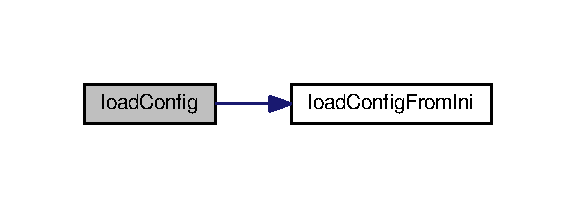
\includegraphics[width=276pt]{configuration_8h_ad5ed6ddd9940c0097cc91774056df1c2_cgraph}
\end{center}
\end{figure}


\hypertarget{configuration_8h_a3cef3589b845d74e6abb41c9d52ada3d}{\index{configuration.\-h@{configuration.\-h}!load\-Config\-From\-Ini@{load\-Config\-From\-Ini}}
\index{load\-Config\-From\-Ini@{load\-Config\-From\-Ini}!configuration.h@{configuration.\-h}}
\subsubsection[{load\-Config\-From\-Ini}]{\setlength{\rightskip}{0pt plus 5cm}{\bf T\-\_\-st\-Config\-Values}$\ast$ load\-Config\-From\-Ini (
\begin{DoxyParamCaption}
\item[{char $\ast$}]{str\-Path}
\end{DoxyParamCaption}
)}}\label{configuration_8h_a3cef3589b845d74e6abb41c9d52ada3d}
\hypertarget{configuration_8h_aa2b23411e3652d16c61db09763bba644}{\index{configuration.\-h@{configuration.\-h}!load\-Environment\-From\-Ini\-File@{load\-Environment\-From\-Ini\-File}}
\index{load\-Environment\-From\-Ini\-File@{load\-Environment\-From\-Ini\-File}!configuration.h@{configuration.\-h}}
\subsubsection[{load\-Environment\-From\-Ini\-File}]{\setlength{\rightskip}{0pt plus 5cm}{\bf T\-\_\-st\-Ini\-Values}$\ast$ load\-Environment\-From\-Ini\-File (
\begin{DoxyParamCaption}
\item[{char $\ast$}]{str\-Path}
\end{DoxyParamCaption}
)}}\label{configuration_8h_aa2b23411e3652d16c61db09763bba644}


Here is the call graph for this function\-:\nopagebreak
\begin{figure}[H]
\begin{center}
\leavevmode
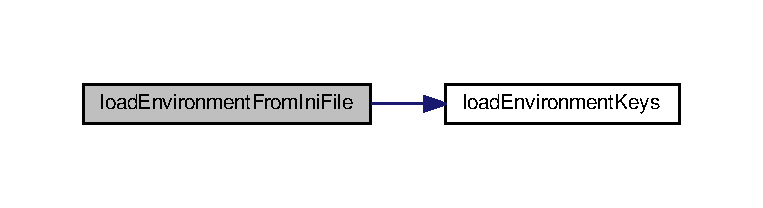
\includegraphics[width=350pt]{configuration_8h_aa2b23411e3652d16c61db09763bba644_cgraph}
\end{center}
\end{figure}


\hypertarget{configuration_8h_a63a188784f1a565b87a789e33f3562b3}{\index{configuration.\-h@{configuration.\-h}!load\-Environment\-From\-Ini\-Memory@{load\-Environment\-From\-Ini\-Memory}}
\index{load\-Environment\-From\-Ini\-Memory@{load\-Environment\-From\-Ini\-Memory}!configuration.h@{configuration.\-h}}
\subsubsection[{load\-Environment\-From\-Ini\-Memory}]{\setlength{\rightskip}{0pt plus 5cm}{\bf T\-\_\-st\-Ini\-Values}$\ast$ load\-Environment\-From\-Ini\-Memory (
\begin{DoxyParamCaption}
\item[{const char $\ast$}]{p\-Buffer, }
\item[{int}]{n\-Size}
\end{DoxyParamCaption}
)}}\label{configuration_8h_a63a188784f1a565b87a789e33f3562b3}


Here is the call graph for this function\-:\nopagebreak
\begin{figure}[H]
\begin{center}
\leavevmode
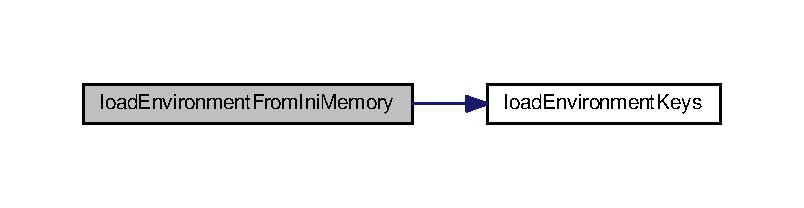
\includegraphics[width=350pt]{configuration_8h_a63a188784f1a565b87a789e33f3562b3_cgraph}
\end{center}
\end{figure}


\hypertarget{configuration_8h_a9e8f363ac5cd9dc04603644592421ac4}{\index{configuration.\-h@{configuration.\-h}!load\-Environment\-Keys@{load\-Environment\-Keys}}
\index{load\-Environment\-Keys@{load\-Environment\-Keys}!configuration.h@{configuration.\-h}}
\subsubsection[{load\-Environment\-Keys}]{\setlength{\rightskip}{0pt plus 5cm}{\bf T\-\_\-st\-Ini\-Values}$\ast$ load\-Environment\-Keys (
\begin{DoxyParamCaption}
\item[{G\-Key\-File $\ast$}]{key\-\_\-file}
\end{DoxyParamCaption}
)}}\label{configuration_8h_a9e8f363ac5cd9dc04603644592421ac4}
Load the .ini file getting the keys associated to the different values that comprises the file. 
\hypertarget{debugMode_8c}{\section{debug\-Mode.\-c File Reference}
\label{debugMode_8c}\index{debug\-Mode.\-c@{debug\-Mode.\-c}}
}
{\ttfamily \#include $<$stdio.\-h$>$}\\*
{\ttfamily \#include $<$stdlib.\-h$>$}\\*
{\ttfamily \#include \char`\"{}Malone.\-h\char`\"{}}\\*
{\ttfamily \#include \char`\"{}printers.\-h\char`\"{}}\\*
{\ttfamily \#include \char`\"{}debug\-Mode.\-h\char`\"{}}\\*
{\ttfamily \#include \char`\"{}tests.\-h\char`\"{}}\\*
{\ttfamily \#include \char`\"{}Auxiliars.\-h\char`\"{}}\\*
{\ttfamily \#include \char`\"{}Env\-File\-Send.\-h\char`\"{}}\\*
{\ttfamily \#include \char`\"{}M\-P\-I\-Data\-Types.\-h\char`\"{}}\\*
{\ttfamily \#include \char`\"{}Monte\-Carlo.\-h\char`\"{}}\\*
{\ttfamily \#include \char`\"{}random\-Elements.\-h\char`\"{}}\\*
Include dependency graph for debug\-Mode.\-c\-:\nopagebreak
\begin{figure}[H]
\begin{center}
\leavevmode
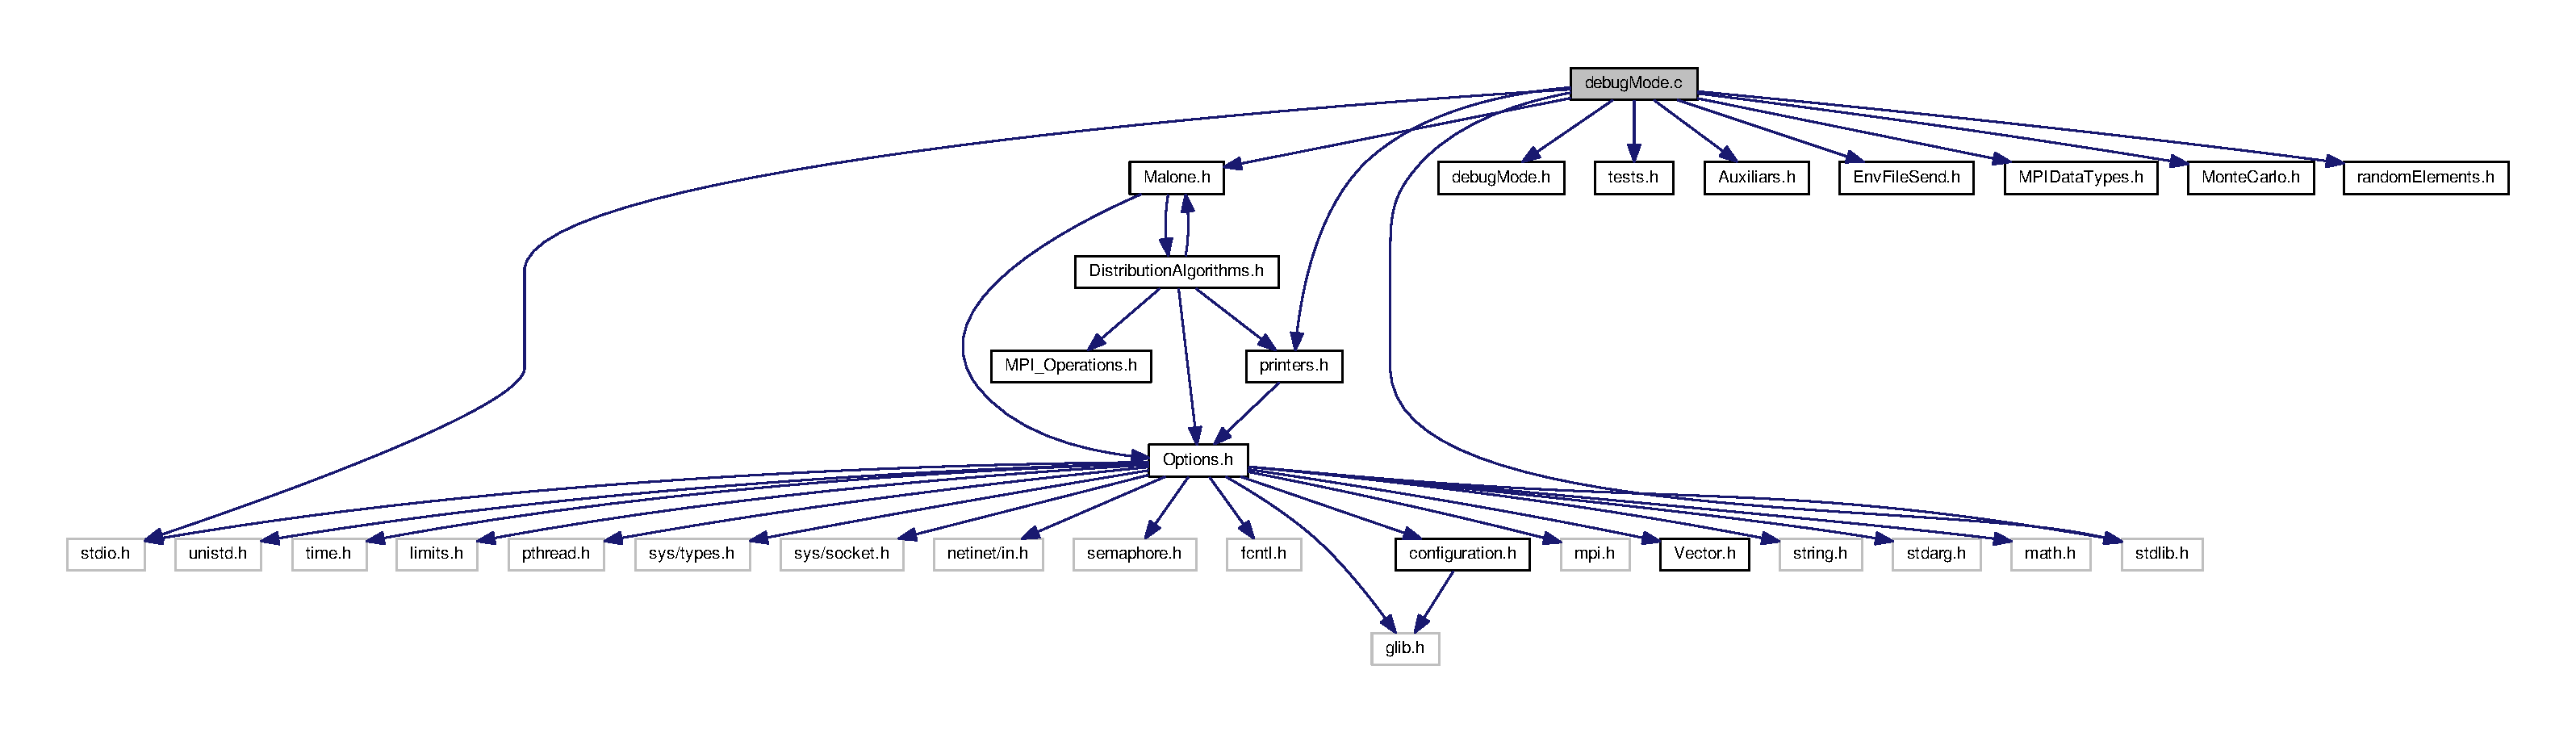
\includegraphics[width=350pt]{debugMode_8c__incl}
\end{center}
\end{figure}
\subsection*{Functions}
\begin{DoxyCompactItemize}
\item 
void \hyperlink{debugMode_8c_a482c287e04f934c64d4fcb2b7c1b604b}{do\-Static\-M\-T} ()
\item 
void \hyperlink{debugMode_8c_a9fe93b9b342b384e80499a781fed2ba8}{do\-Pirata} ()
\item 
void \hyperlink{debugMode_8c_a0d67107183d290268bda8ebe8954be3d}{master\-Debug\-Operations} ()
\item 
void \hyperlink{debugMode_8c_afc59696cc466e8ac6ed689e8ce5d06a3}{workers\-Debug\-Operations} ()
\item 
void \hyperlink{debugMode_8c_a32b2c9b1135380309df9fff94b55dc15}{launch\-Debug\-Mode} ()
\end{DoxyCompactItemize}


\subsection{Function Documentation}
\hypertarget{debugMode_8c_a9fe93b9b342b384e80499a781fed2ba8}{\index{debug\-Mode.\-c@{debug\-Mode.\-c}!do\-Pirata@{do\-Pirata}}
\index{do\-Pirata@{do\-Pirata}!debugMode.c@{debug\-Mode.\-c}}
\subsubsection[{do\-Pirata}]{\setlength{\rightskip}{0pt plus 5cm}void do\-Pirata (
\begin{DoxyParamCaption}
{}
\end{DoxyParamCaption}
)}}\label{debugMode_8c_a9fe93b9b342b384e80499a781fed2ba8}


Here is the call graph for this function\-:\nopagebreak
\begin{figure}[H]
\begin{center}
\leavevmode
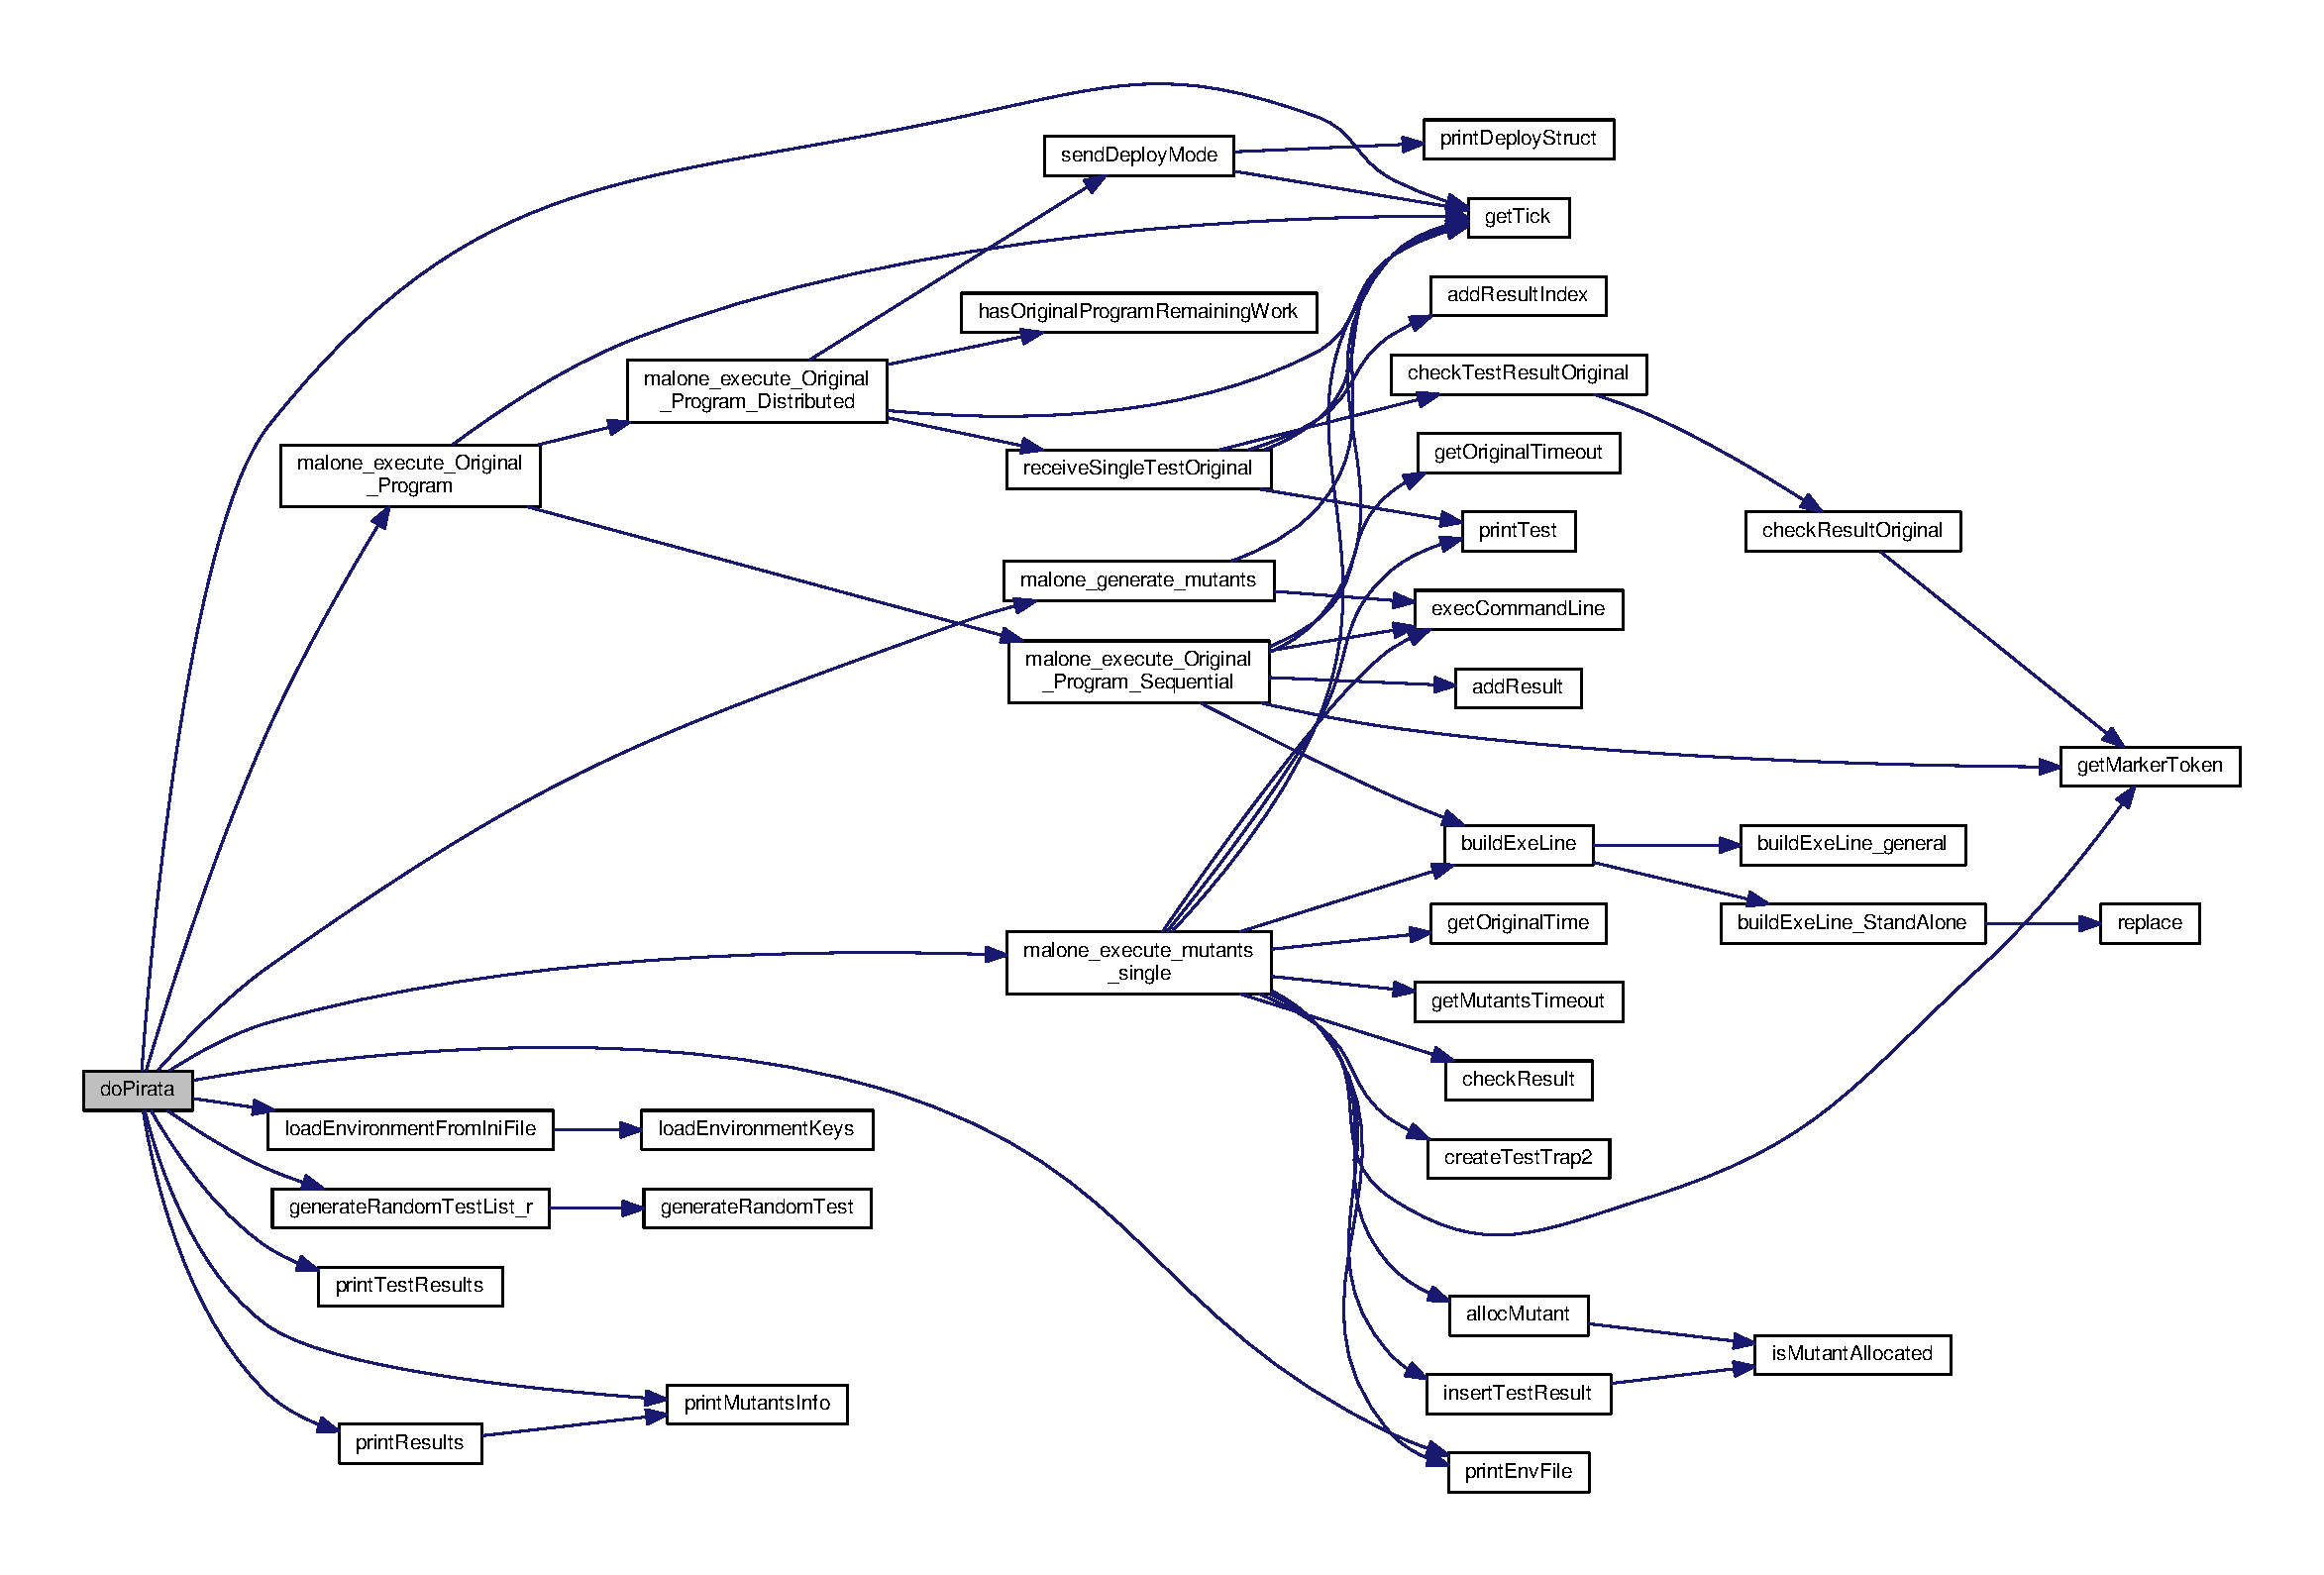
\includegraphics[width=350pt]{debugMode_8c_a9fe93b9b342b384e80499a781fed2ba8_cgraph}
\end{center}
\end{figure}


\hypertarget{debugMode_8c_a482c287e04f934c64d4fcb2b7c1b604b}{\index{debug\-Mode.\-c@{debug\-Mode.\-c}!do\-Static\-M\-T@{do\-Static\-M\-T}}
\index{do\-Static\-M\-T@{do\-Static\-M\-T}!debugMode.c@{debug\-Mode.\-c}}
\subsubsection[{do\-Static\-M\-T}]{\setlength{\rightskip}{0pt plus 5cm}void do\-Static\-M\-T (
\begin{DoxyParamCaption}
{}
\end{DoxyParamCaption}
)}}\label{debugMode_8c_a482c287e04f934c64d4fcb2b7c1b604b}


Here is the call graph for this function\-:\nopagebreak
\begin{figure}[H]
\begin{center}
\leavevmode
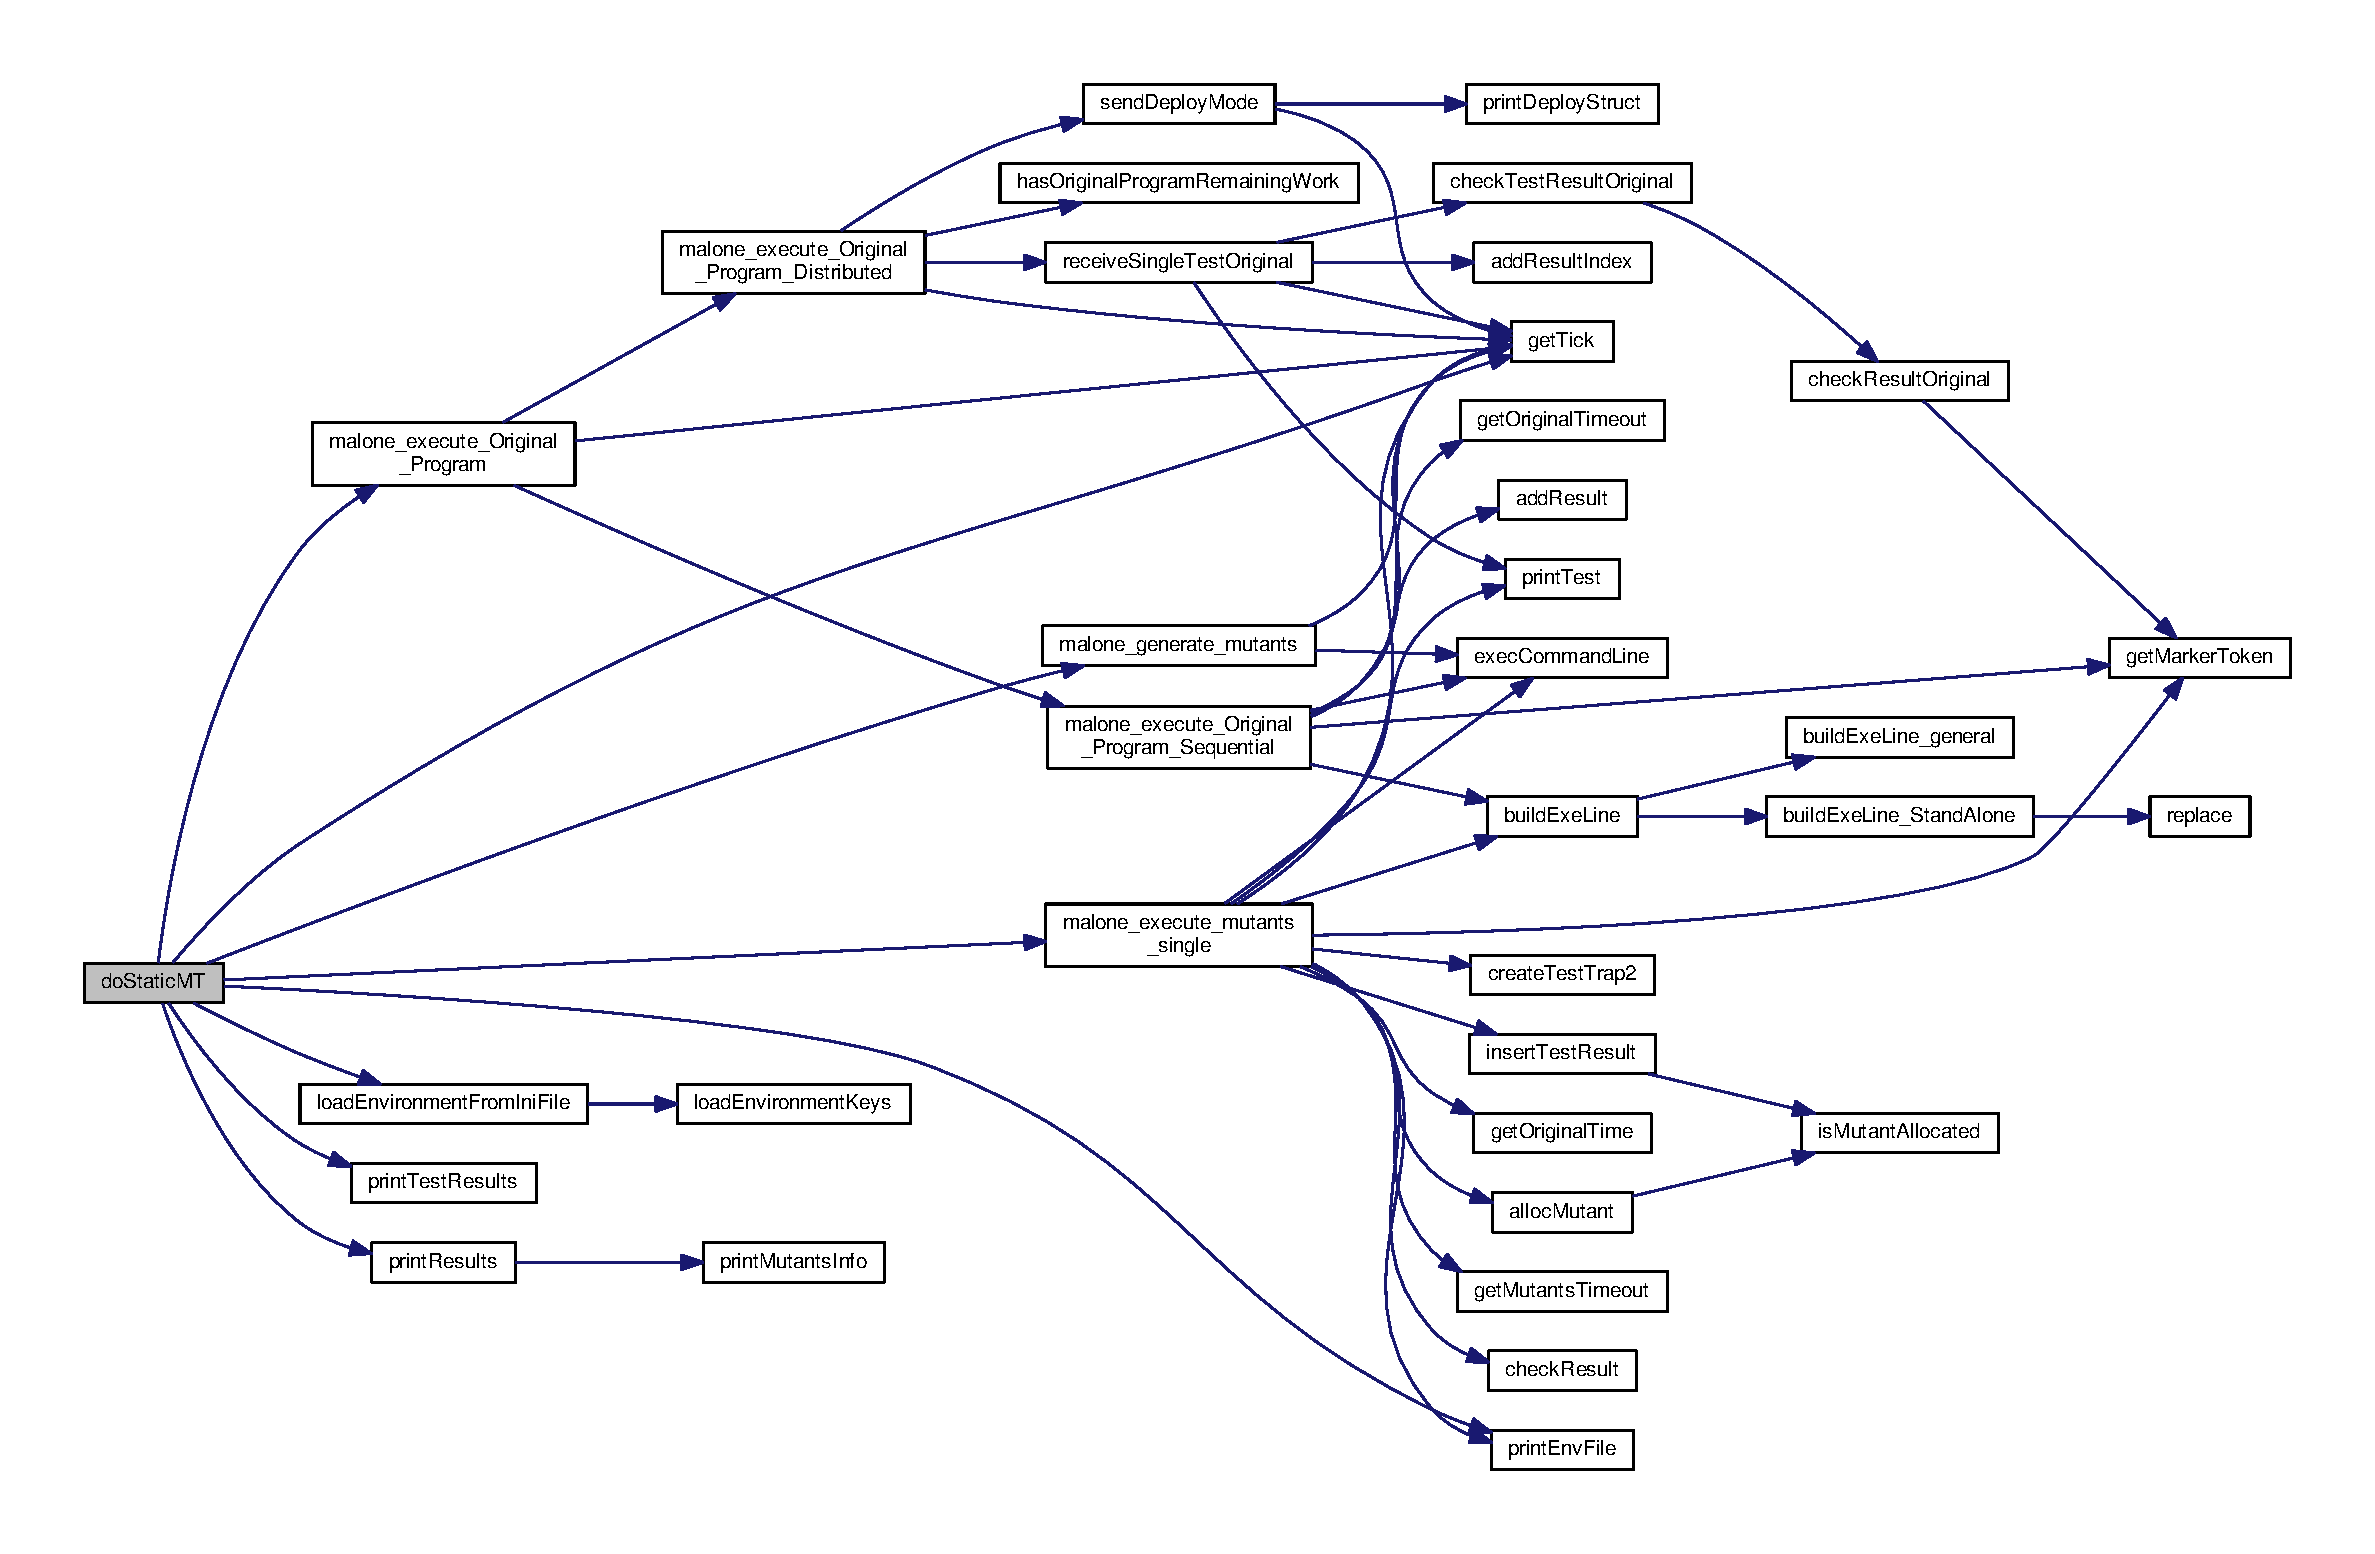
\includegraphics[width=350pt]{debugMode_8c_a482c287e04f934c64d4fcb2b7c1b604b_cgraph}
\end{center}
\end{figure}


\hypertarget{debugMode_8c_a32b2c9b1135380309df9fff94b55dc15}{\index{debug\-Mode.\-c@{debug\-Mode.\-c}!launch\-Debug\-Mode@{launch\-Debug\-Mode}}
\index{launch\-Debug\-Mode@{launch\-Debug\-Mode}!debugMode.c@{debug\-Mode.\-c}}
\subsubsection[{launch\-Debug\-Mode}]{\setlength{\rightskip}{0pt plus 5cm}void launch\-Debug\-Mode (
\begin{DoxyParamCaption}
{}
\end{DoxyParamCaption}
)}}\label{debugMode_8c_a32b2c9b1135380309df9fff94b55dc15}


Here is the call graph for this function\-:\nopagebreak
\begin{figure}[H]
\begin{center}
\leavevmode
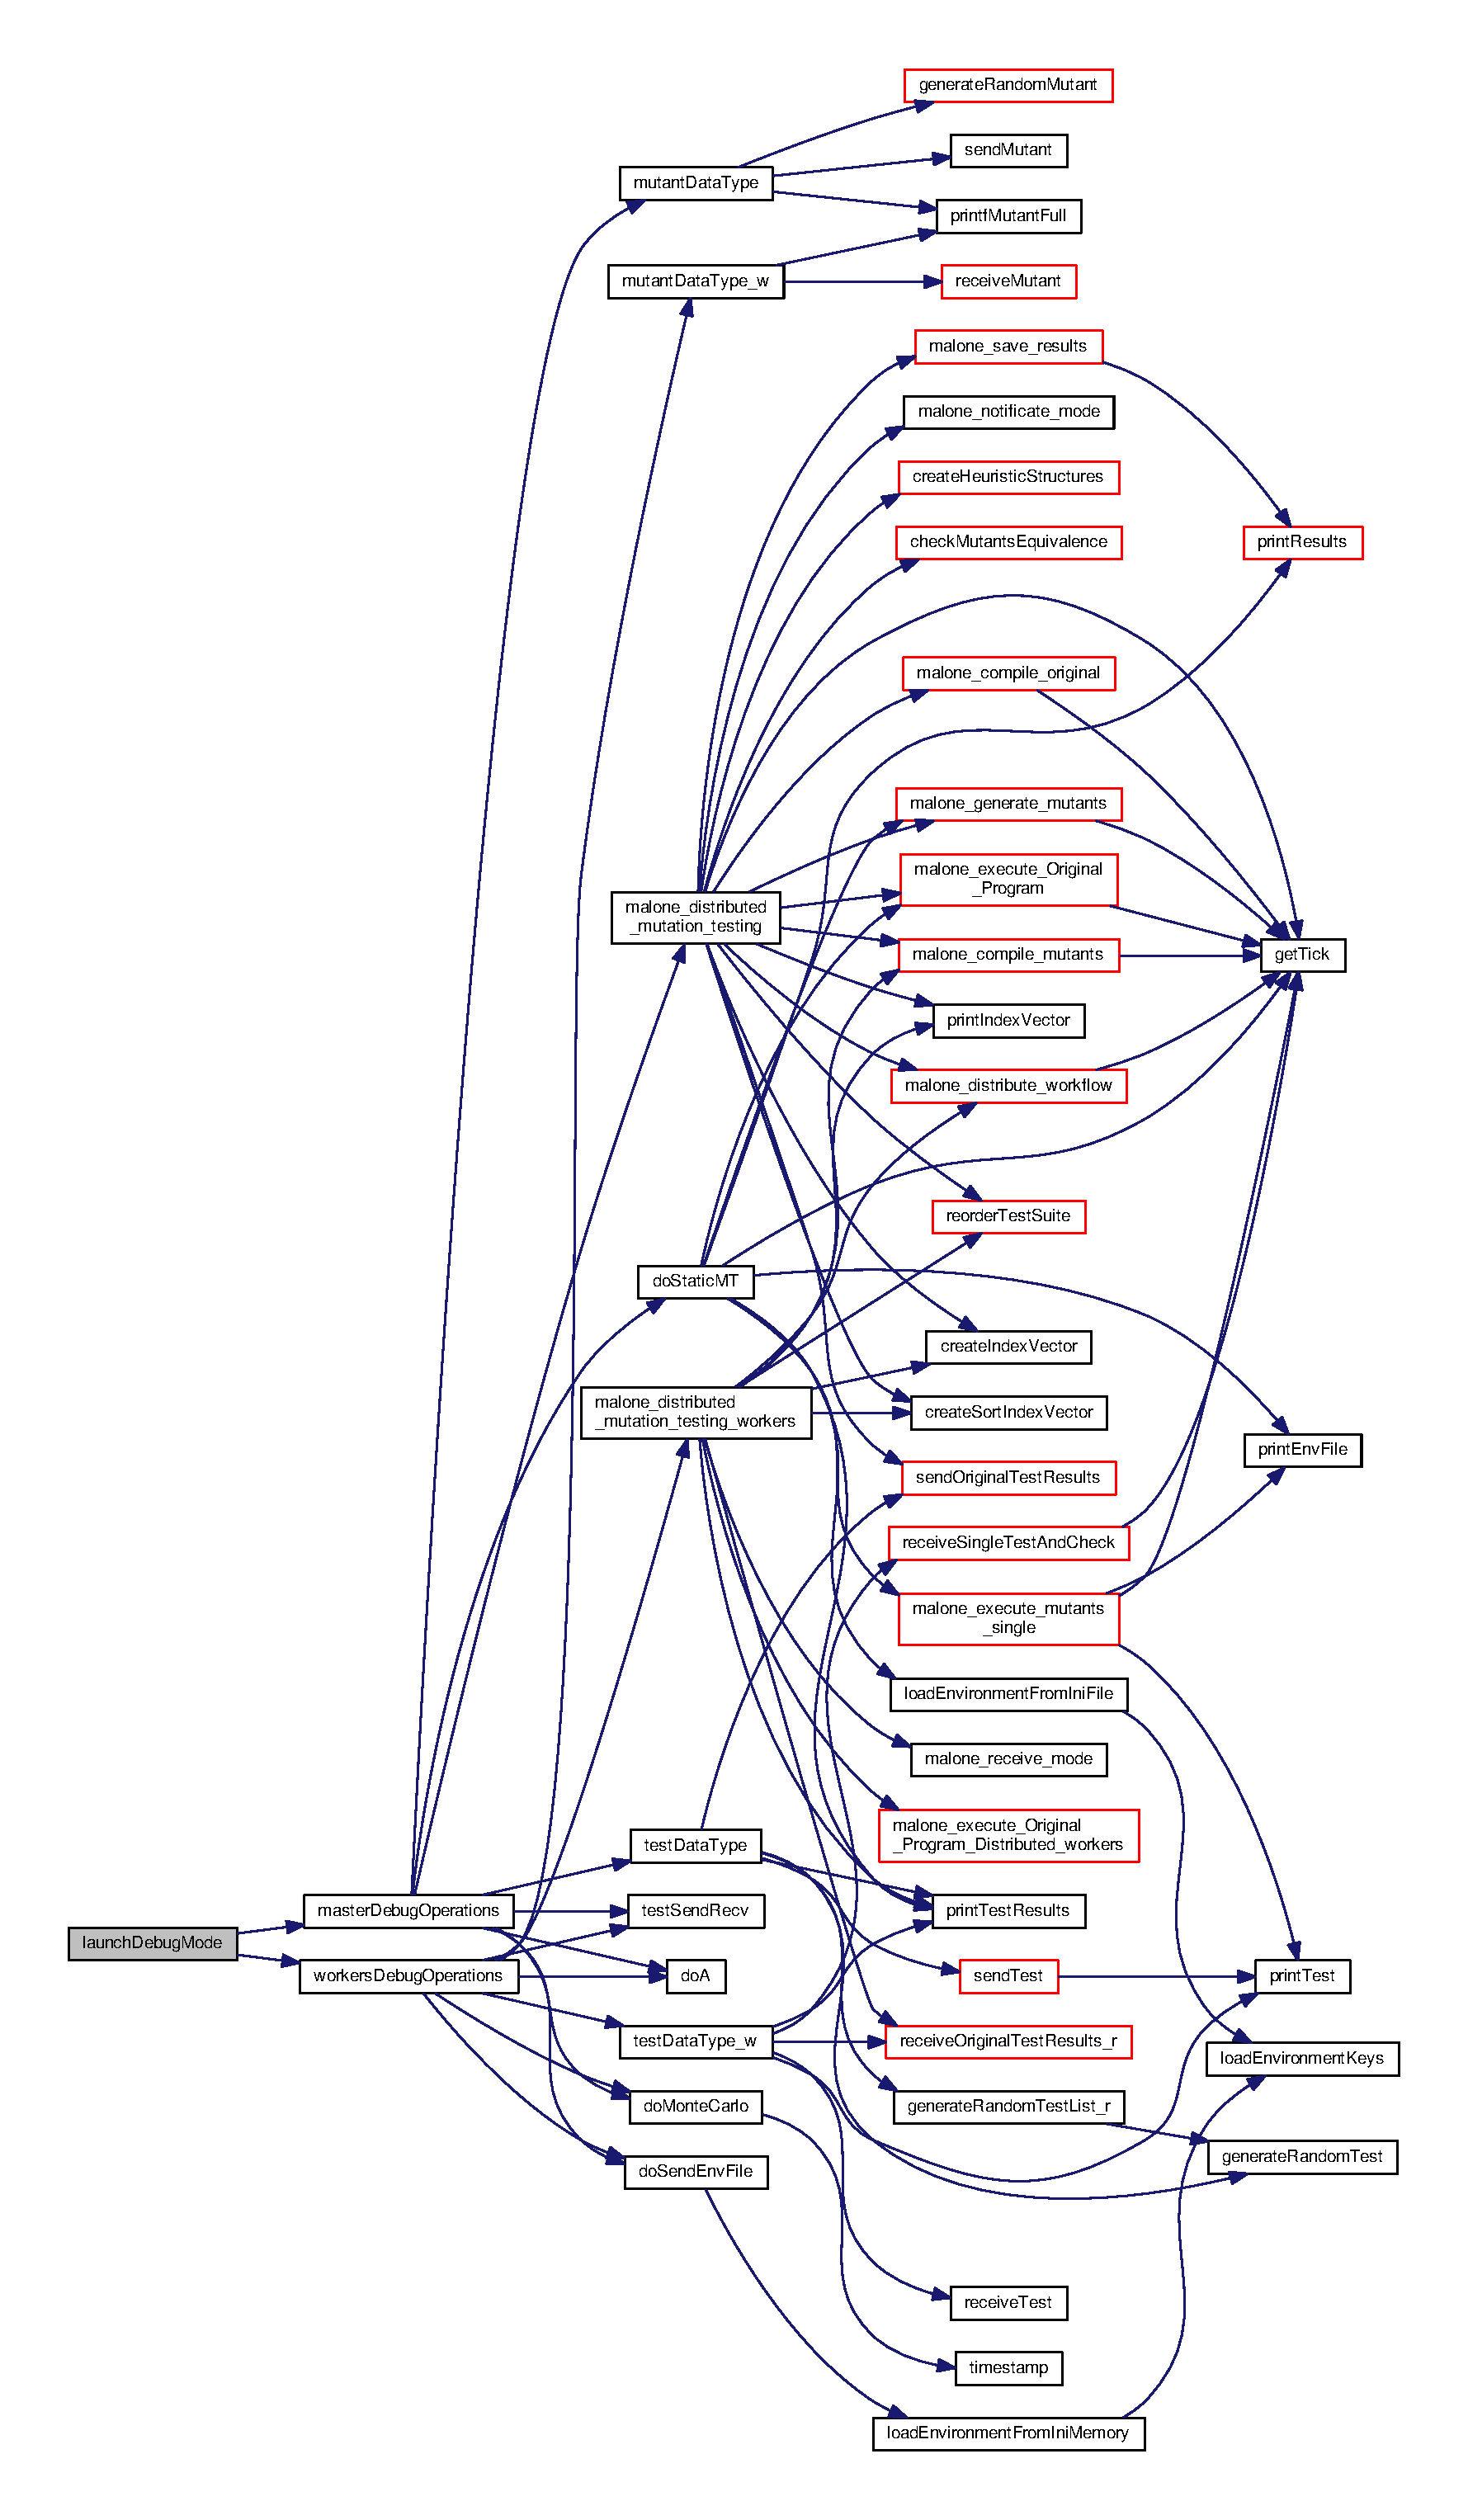
\includegraphics[height=550pt]{debugMode_8c_a32b2c9b1135380309df9fff94b55dc15_cgraph}
\end{center}
\end{figure}


\hypertarget{debugMode_8c_a0d67107183d290268bda8ebe8954be3d}{\index{debug\-Mode.\-c@{debug\-Mode.\-c}!master\-Debug\-Operations@{master\-Debug\-Operations}}
\index{master\-Debug\-Operations@{master\-Debug\-Operations}!debugMode.c@{debug\-Mode.\-c}}
\subsubsection[{master\-Debug\-Operations}]{\setlength{\rightskip}{0pt plus 5cm}void master\-Debug\-Operations (
\begin{DoxyParamCaption}
{}
\end{DoxyParamCaption}
)}}\label{debugMode_8c_a0d67107183d290268bda8ebe8954be3d}


Here is the call graph for this function\-:\nopagebreak
\begin{figure}[H]
\begin{center}
\leavevmode
\includegraphics[width=350pt]{debugMode_8c_a0d67107183d290268bda8ebe8954be3d_cgraph}
\end{center}
\end{figure}


\hypertarget{debugMode_8c_afc59696cc466e8ac6ed689e8ce5d06a3}{\index{debug\-Mode.\-c@{debug\-Mode.\-c}!workers\-Debug\-Operations@{workers\-Debug\-Operations}}
\index{workers\-Debug\-Operations@{workers\-Debug\-Operations}!debugMode.c@{debug\-Mode.\-c}}
\subsubsection[{workers\-Debug\-Operations}]{\setlength{\rightskip}{0pt plus 5cm}void workers\-Debug\-Operations (
\begin{DoxyParamCaption}
{}
\end{DoxyParamCaption}
)}}\label{debugMode_8c_afc59696cc466e8ac6ed689e8ce5d06a3}


Here is the call graph for this function\-:\nopagebreak
\begin{figure}[H]
\begin{center}
\leavevmode
\includegraphics[width=350pt]{debugMode_8c_afc59696cc466e8ac6ed689e8ce5d06a3_cgraph}
\end{center}
\end{figure}



\hypertarget{debugMode_8h}{\section{debug\-Mode.\-h File Reference}
\label{debugMode_8h}\index{debug\-Mode.\-h@{debug\-Mode.\-h}}
}
This graph shows which files directly or indirectly include this file\-:\nopagebreak
\begin{figure}[H]
\begin{center}
\leavevmode
\includegraphics[width=328pt]{debugMode_8h__dep__incl}
\end{center}
\end{figure}
\subsection*{Functions}
\begin{DoxyCompactItemize}
\item 
void \hyperlink{debugMode_8h_a32b2c9b1135380309df9fff94b55dc15}{launch\-Debug\-Mode} ()
\item 
void \hyperlink{debugMode_8h_afc59696cc466e8ac6ed689e8ce5d06a3}{workers\-Debug\-Operations} ()
\item 
void \hyperlink{debugMode_8h_a0d67107183d290268bda8ebe8954be3d}{master\-Debug\-Operations} ()
\item 
void \hyperlink{debugMode_8h_a482c287e04f934c64d4fcb2b7c1b604b}{do\-Static\-M\-T} ()
\item 
void \hyperlink{debugMode_8h_a9fe93b9b342b384e80499a781fed2ba8}{do\-Pirata} ()
\end{DoxyCompactItemize}


\subsection{Function Documentation}
\hypertarget{debugMode_8h_a9fe93b9b342b384e80499a781fed2ba8}{\index{debug\-Mode.\-h@{debug\-Mode.\-h}!do\-Pirata@{do\-Pirata}}
\index{do\-Pirata@{do\-Pirata}!debugMode.h@{debug\-Mode.\-h}}
\subsubsection[{do\-Pirata}]{\setlength{\rightskip}{0pt plus 5cm}void do\-Pirata (
\begin{DoxyParamCaption}
{}
\end{DoxyParamCaption}
)}}\label{debugMode_8h_a9fe93b9b342b384e80499a781fed2ba8}


Here is the call graph for this function\-:\nopagebreak
\begin{figure}[H]
\begin{center}
\leavevmode
\includegraphics[width=350pt]{debugMode_8h_a9fe93b9b342b384e80499a781fed2ba8_cgraph}
\end{center}
\end{figure}


\hypertarget{debugMode_8h_a482c287e04f934c64d4fcb2b7c1b604b}{\index{debug\-Mode.\-h@{debug\-Mode.\-h}!do\-Static\-M\-T@{do\-Static\-M\-T}}
\index{do\-Static\-M\-T@{do\-Static\-M\-T}!debugMode.h@{debug\-Mode.\-h}}
\subsubsection[{do\-Static\-M\-T}]{\setlength{\rightskip}{0pt plus 5cm}void do\-Static\-M\-T (
\begin{DoxyParamCaption}
{}
\end{DoxyParamCaption}
)}}\label{debugMode_8h_a482c287e04f934c64d4fcb2b7c1b604b}


Here is the call graph for this function\-:\nopagebreak
\begin{figure}[H]
\begin{center}
\leavevmode
\includegraphics[width=350pt]{debugMode_8h_a482c287e04f934c64d4fcb2b7c1b604b_cgraph}
\end{center}
\end{figure}


\hypertarget{debugMode_8h_a32b2c9b1135380309df9fff94b55dc15}{\index{debug\-Mode.\-h@{debug\-Mode.\-h}!launch\-Debug\-Mode@{launch\-Debug\-Mode}}
\index{launch\-Debug\-Mode@{launch\-Debug\-Mode}!debugMode.h@{debug\-Mode.\-h}}
\subsubsection[{launch\-Debug\-Mode}]{\setlength{\rightskip}{0pt plus 5cm}void launch\-Debug\-Mode (
\begin{DoxyParamCaption}
{}
\end{DoxyParamCaption}
)}}\label{debugMode_8h_a32b2c9b1135380309df9fff94b55dc15}


Here is the call graph for this function\-:\nopagebreak
\begin{figure}[H]
\begin{center}
\leavevmode
\includegraphics[height=550pt]{debugMode_8h_a32b2c9b1135380309df9fff94b55dc15_cgraph}
\end{center}
\end{figure}


\hypertarget{debugMode_8h_a0d67107183d290268bda8ebe8954be3d}{\index{debug\-Mode.\-h@{debug\-Mode.\-h}!master\-Debug\-Operations@{master\-Debug\-Operations}}
\index{master\-Debug\-Operations@{master\-Debug\-Operations}!debugMode.h@{debug\-Mode.\-h}}
\subsubsection[{master\-Debug\-Operations}]{\setlength{\rightskip}{0pt plus 5cm}void master\-Debug\-Operations (
\begin{DoxyParamCaption}
{}
\end{DoxyParamCaption}
)}}\label{debugMode_8h_a0d67107183d290268bda8ebe8954be3d}


Here is the call graph for this function\-:\nopagebreak
\begin{figure}[H]
\begin{center}
\leavevmode
\includegraphics[width=350pt]{debugMode_8h_a0d67107183d290268bda8ebe8954be3d_cgraph}
\end{center}
\end{figure}


\hypertarget{debugMode_8h_afc59696cc466e8ac6ed689e8ce5d06a3}{\index{debug\-Mode.\-h@{debug\-Mode.\-h}!workers\-Debug\-Operations@{workers\-Debug\-Operations}}
\index{workers\-Debug\-Operations@{workers\-Debug\-Operations}!debugMode.h@{debug\-Mode.\-h}}
\subsubsection[{workers\-Debug\-Operations}]{\setlength{\rightskip}{0pt plus 5cm}void workers\-Debug\-Operations (
\begin{DoxyParamCaption}
{}
\end{DoxyParamCaption}
)}}\label{debugMode_8h_afc59696cc466e8ac6ed689e8ce5d06a3}


Here is the call graph for this function\-:\nopagebreak
\begin{figure}[H]
\begin{center}
\leavevmode
\includegraphics[width=350pt]{debugMode_8h_afc59696cc466e8ac6ed689e8ce5d06a3_cgraph}
\end{center}
\end{figure}



\hypertarget{distribution__adaptive__grain_8c}{\section{distribution\-\_\-adaptive\-\_\-grain.\-c File Reference}
\label{distribution__adaptive__grain_8c}\index{distribution\-\_\-adaptive\-\_\-grain.\-c@{distribution\-\_\-adaptive\-\_\-grain.\-c}}
}
{\ttfamily \#include \char`\"{}Distribution\-Algorithms.\-h\char`\"{}}\\*
{\ttfamily \#include \char`\"{}Auxiliars.\-h\char`\"{}}\\*
Include dependency graph for distribution\-\_\-adaptive\-\_\-grain.\-c\-:\nopagebreak
\begin{figure}[H]
\begin{center}
\leavevmode
\includegraphics[width=350pt]{distribution__adaptive__grain_8c__incl}
\end{center}
\end{figure}
\subsection*{Macros}
\begin{DoxyCompactItemize}
\item 
\#define \hyperlink{distribution__adaptive__grain_8c_a07167db89abd1c44007b1de1a00f335c}{M\-I\-N\-I\-M\-U\-M\-\_\-\-M\-U\-T\-A\-N\-T\-S}~\hyperlink{Options_8h_a21f93b549e3bccb6cb16b43c2ea44d6a}{m\-\_\-n\-Size}-\/1
\end{DoxyCompactItemize}
\subsection*{Functions}
\begin{DoxyCompactItemize}
\item 
int \hyperlink{distribution__adaptive__grain_8c_a709a710adb0ee53ce85adc6c59c12494}{distribution\-\_\-adaptive\-\_\-grain\-\_\-scatter} (\hyperlink{Options_8h_a8859326946ba85db44b56cab4ce88aff}{T\-\_\-e\-Execution\-Mode} e\-Method)
\item 
int \hyperlink{distribution__adaptive__grain_8c_a0f70ea863f88a7edefd48759a7780036}{update\-Counters\-\_\-adaptive} (\hyperlink{structT__stExecutionMap}{T\-\_\-st\-Execution\-Map} $\ast$exe\-Map, \hyperlink{structT__stExecutionStructure}{T\-\_\-st\-Execution\-Structure} $\ast$exe\-Worker, int $\ast$n\-Index\-Test\-Init, int $\ast$n\-Index\-Test\-End, int $\ast$n\-Index\-Mutant\-Init, int $\ast$n\-Index\-Mutant\-End)
\item 
int \hyperlink{distribution__adaptive__grain_8c_a6aa203b510604838013c32fa45670bbc}{check\-Mutants\-Alive} (\hyperlink{structMutantList}{Mutant\-List} $\ast$p\-Mutant\-List)
\item 
void \hyperlink{distribution__adaptive__grain_8c_aa606a467f04ac00cc1062f82100c2de8}{update\-Kill\-Mutant\-\_\-adaptive} (\hyperlink{structT__stExecutionMap}{T\-\_\-st\-Execution\-Map} $\ast$exe\-Map, \hyperlink{structT__stExecutionStructure}{T\-\_\-st\-Execution\-Structure} $\ast$exe\-Worker, \hyperlink{structMutantList}{Mutant\-List} $\ast$p\-Mutant\-List)
\end{DoxyCompactItemize}


\subsection{Macro Definition Documentation}
\hypertarget{distribution__adaptive__grain_8c_a07167db89abd1c44007b1de1a00f335c}{\index{distribution\-\_\-adaptive\-\_\-grain.\-c@{distribution\-\_\-adaptive\-\_\-grain.\-c}!M\-I\-N\-I\-M\-U\-M\-\_\-\-M\-U\-T\-A\-N\-T\-S@{M\-I\-N\-I\-M\-U\-M\-\_\-\-M\-U\-T\-A\-N\-T\-S}}
\index{M\-I\-N\-I\-M\-U\-M\-\_\-\-M\-U\-T\-A\-N\-T\-S@{M\-I\-N\-I\-M\-U\-M\-\_\-\-M\-U\-T\-A\-N\-T\-S}!distribution_adaptive_grain.c@{distribution\-\_\-adaptive\-\_\-grain.\-c}}
\subsubsection[{M\-I\-N\-I\-M\-U\-M\-\_\-\-M\-U\-T\-A\-N\-T\-S}]{\setlength{\rightskip}{0pt plus 5cm}\#define M\-I\-N\-I\-M\-U\-M\-\_\-\-M\-U\-T\-A\-N\-T\-S~{\bf m\-\_\-n\-Size}-\/1}}\label{distribution__adaptive__grain_8c_a07167db89abd1c44007b1de1a00f335c}


\subsection{Function Documentation}
\hypertarget{distribution__adaptive__grain_8c_a6aa203b510604838013c32fa45670bbc}{\index{distribution\-\_\-adaptive\-\_\-grain.\-c@{distribution\-\_\-adaptive\-\_\-grain.\-c}!check\-Mutants\-Alive@{check\-Mutants\-Alive}}
\index{check\-Mutants\-Alive@{check\-Mutants\-Alive}!distribution_adaptive_grain.c@{distribution\-\_\-adaptive\-\_\-grain.\-c}}
\subsubsection[{check\-Mutants\-Alive}]{\setlength{\rightskip}{0pt plus 5cm}int check\-Mutants\-Alive (
\begin{DoxyParamCaption}
\item[{{\bf Mutant\-List} $\ast$}]{p\-Mutant\-List}
\end{DoxyParamCaption}
)}}\label{distribution__adaptive__grain_8c_a6aa203b510604838013c32fa45670bbc}
\hypertarget{distribution__adaptive__grain_8c_a709a710adb0ee53ce85adc6c59c12494}{\index{distribution\-\_\-adaptive\-\_\-grain.\-c@{distribution\-\_\-adaptive\-\_\-grain.\-c}!distribution\-\_\-adaptive\-\_\-grain\-\_\-scatter@{distribution\-\_\-adaptive\-\_\-grain\-\_\-scatter}}
\index{distribution\-\_\-adaptive\-\_\-grain\-\_\-scatter@{distribution\-\_\-adaptive\-\_\-grain\-\_\-scatter}!distribution_adaptive_grain.c@{distribution\-\_\-adaptive\-\_\-grain.\-c}}
\subsubsection[{distribution\-\_\-adaptive\-\_\-grain\-\_\-scatter}]{\setlength{\rightskip}{0pt plus 5cm}int distribution\-\_\-adaptive\-\_\-grain\-\_\-scatter (
\begin{DoxyParamCaption}
\item[{{\bf T\-\_\-e\-Execution\-Mode}}]{e\-Method}
\end{DoxyParamCaption}
)}}\label{distribution__adaptive__grain_8c_a709a710adb0ee53ce85adc6c59c12494}
This distribution takes advance of two previous algorithms\-: dynamic\-\_\-mutants and full\-\_\-fynamic\-\_\-scatter. As a result, we present a mixed algorithm which changes the size of the execution grain depending on the remaining workload. 
\begin{DoxyParams}{Parameters}
{\em e\-Method} & \\
\hline
\end{DoxyParams}
\begin{DoxyReturn}{Returns}

\end{DoxyReturn}


Here is the call graph for this function\-:\nopagebreak
\begin{figure}[H]
\begin{center}
\leavevmode
\includegraphics[width=350pt]{distribution__adaptive__grain_8c_a709a710adb0ee53ce85adc6c59c12494_cgraph}
\end{center}
\end{figure}


\hypertarget{distribution__adaptive__grain_8c_a0f70ea863f88a7edefd48759a7780036}{\index{distribution\-\_\-adaptive\-\_\-grain.\-c@{distribution\-\_\-adaptive\-\_\-grain.\-c}!update\-Counters\-\_\-adaptive@{update\-Counters\-\_\-adaptive}}
\index{update\-Counters\-\_\-adaptive@{update\-Counters\-\_\-adaptive}!distribution_adaptive_grain.c@{distribution\-\_\-adaptive\-\_\-grain.\-c}}
\subsubsection[{update\-Counters\-\_\-adaptive}]{\setlength{\rightskip}{0pt plus 5cm}int update\-Counters\-\_\-adaptive (
\begin{DoxyParamCaption}
\item[{{\bf T\-\_\-st\-Execution\-Map} $\ast$}]{exe\-Map, }
\item[{{\bf T\-\_\-st\-Execution\-Structure} $\ast$}]{exe\-Worker, }
\item[{int $\ast$}]{n\-Index\-Test\-Init, }
\item[{int $\ast$}]{n\-Index\-Test\-End, }
\item[{int $\ast$}]{n\-Index\-Mutant\-Init, }
\item[{int $\ast$}]{n\-Index\-Mutant\-End}
\end{DoxyParamCaption}
)}}\label{distribution__adaptive__grain_8c_a0f70ea863f88a7edefd48759a7780036}
\hypertarget{distribution__adaptive__grain_8c_aa606a467f04ac00cc1062f82100c2de8}{\index{distribution\-\_\-adaptive\-\_\-grain.\-c@{distribution\-\_\-adaptive\-\_\-grain.\-c}!update\-Kill\-Mutant\-\_\-adaptive@{update\-Kill\-Mutant\-\_\-adaptive}}
\index{update\-Kill\-Mutant\-\_\-adaptive@{update\-Kill\-Mutant\-\_\-adaptive}!distribution_adaptive_grain.c@{distribution\-\_\-adaptive\-\_\-grain.\-c}}
\subsubsection[{update\-Kill\-Mutant\-\_\-adaptive}]{\setlength{\rightskip}{0pt plus 5cm}void update\-Kill\-Mutant\-\_\-adaptive (
\begin{DoxyParamCaption}
\item[{{\bf T\-\_\-st\-Execution\-Map} $\ast$}]{exe\-Map, }
\item[{{\bf T\-\_\-st\-Execution\-Structure} $\ast$}]{exe\-Worker, }
\item[{{\bf Mutant\-List} $\ast$}]{p\-Mutant\-List}
\end{DoxyParamCaption}
)}}\label{distribution__adaptive__grain_8c_aa606a467f04ac00cc1062f82100c2de8}

\hypertarget{distribution__dynamic__mutants_8c}{\section{distribution\-\_\-dynamic\-\_\-mutants.\-c File Reference}
\label{distribution__dynamic__mutants_8c}\index{distribution\-\_\-dynamic\-\_\-mutants.\-c@{distribution\-\_\-dynamic\-\_\-mutants.\-c}}
}
{\ttfamily \#include \char`\"{}Distribution\-Algorithms.\-h\char`\"{}}\\*
Include dependency graph for distribution\-\_\-dynamic\-\_\-mutants.\-c\-:\nopagebreak
\begin{figure}[H]
\begin{center}
\leavevmode
\includegraphics[width=350pt]{distribution__dynamic__mutants_8c__incl}
\end{center}
\end{figure}
\subsection*{Functions}
\begin{DoxyCompactItemize}
\item 
int \hyperlink{distribution__dynamic__mutants_8c_a40b5a6d681374f437bb73c2d31d08c0d}{distribution\-\_\-dynamic\-\_\-mutants} (\hyperlink{Options_8h_a8859326946ba85db44b56cab4ce88aff}{T\-\_\-e\-Execution\-Mode} e\-Method)
\end{DoxyCompactItemize}


\subsection{Function Documentation}
\hypertarget{distribution__dynamic__mutants_8c_a40b5a6d681374f437bb73c2d31d08c0d}{\index{distribution\-\_\-dynamic\-\_\-mutants.\-c@{distribution\-\_\-dynamic\-\_\-mutants.\-c}!distribution\-\_\-dynamic\-\_\-mutants@{distribution\-\_\-dynamic\-\_\-mutants}}
\index{distribution\-\_\-dynamic\-\_\-mutants@{distribution\-\_\-dynamic\-\_\-mutants}!distribution_dynamic_mutants.c@{distribution\-\_\-dynamic\-\_\-mutants.\-c}}
\subsubsection[{distribution\-\_\-dynamic\-\_\-mutants}]{\setlength{\rightskip}{0pt plus 5cm}int distribution\-\_\-dynamic\-\_\-mutants (
\begin{DoxyParamCaption}
\item[{{\bf T\-\_\-e\-Execution\-Mode}}]{e\-Method}
\end{DoxyParamCaption}
)}}\label{distribution__dynamic__mutants_8c_a40b5a6d681374f437bb73c2d31d08c0d}


Here is the call graph for this function\-:\nopagebreak
\begin{figure}[H]
\begin{center}
\leavevmode
\includegraphics[width=350pt]{distribution__dynamic__mutants_8c_a40b5a6d681374f437bb73c2d31d08c0d_cgraph}
\end{center}
\end{figure}



\hypertarget{distribution__full__dynamic_8c}{\section{distribution\-\_\-full\-\_\-dynamic.\-c File Reference}
\label{distribution__full__dynamic_8c}\index{distribution\-\_\-full\-\_\-dynamic.\-c@{distribution\-\_\-full\-\_\-dynamic.\-c}}
}
{\ttfamily \#include \char`\"{}Distribution\-Algorithms.\-h\char`\"{}}\\*
Include dependency graph for distribution\-\_\-full\-\_\-dynamic.\-c\-:\nopagebreak
\begin{figure}[H]
\begin{center}
\leavevmode
\includegraphics[width=350pt]{distribution__full__dynamic_8c__incl}
\end{center}
\end{figure}
\subsection*{Functions}
\begin{DoxyCompactItemize}
\item 
int \hyperlink{distribution__full__dynamic_8c_aaaab88163670001aef0e78bfc18c032e}{distribution\-\_\-full\-\_\-dynamic} (\hyperlink{Options_8h_a8859326946ba85db44b56cab4ce88aff}{T\-\_\-e\-Execution\-Mode} e\-Method)
\end{DoxyCompactItemize}


\subsection{Function Documentation}
\hypertarget{distribution__full__dynamic_8c_aaaab88163670001aef0e78bfc18c032e}{\index{distribution\-\_\-full\-\_\-dynamic.\-c@{distribution\-\_\-full\-\_\-dynamic.\-c}!distribution\-\_\-full\-\_\-dynamic@{distribution\-\_\-full\-\_\-dynamic}}
\index{distribution\-\_\-full\-\_\-dynamic@{distribution\-\_\-full\-\_\-dynamic}!distribution_full_dynamic.c@{distribution\-\_\-full\-\_\-dynamic.\-c}}
\subsubsection[{distribution\-\_\-full\-\_\-dynamic}]{\setlength{\rightskip}{0pt plus 5cm}int distribution\-\_\-full\-\_\-dynamic (
\begin{DoxyParamCaption}
\item[{{\bf T\-\_\-e\-Execution\-Mode}}]{e\-Method}
\end{DoxyParamCaption}
)}}\label{distribution__full__dynamic_8c_aaaab88163670001aef0e78bfc18c032e}


Here is the call graph for this function\-:\nopagebreak
\begin{figure}[H]
\begin{center}
\leavevmode
\includegraphics[width=350pt]{distribution__full__dynamic_8c_aaaab88163670001aef0e78bfc18c032e_cgraph}
\end{center}
\end{figure}



\hypertarget{distribution__full__dynamic__scatter_8c}{\section{distribution\-\_\-full\-\_\-dynamic\-\_\-scatter.\-c File Reference}
\label{distribution__full__dynamic__scatter_8c}\index{distribution\-\_\-full\-\_\-dynamic\-\_\-scatter.\-c@{distribution\-\_\-full\-\_\-dynamic\-\_\-scatter.\-c}}
}
{\ttfamily \#include \char`\"{}Distribution\-Algorithms.\-h\char`\"{}}\\*
Include dependency graph for distribution\-\_\-full\-\_\-dynamic\-\_\-scatter.\-c\-:\nopagebreak
\begin{figure}[H]
\begin{center}
\leavevmode
\includegraphics[width=350pt]{distribution__full__dynamic__scatter_8c__incl}
\end{center}
\end{figure}
\subsection*{Functions}
\begin{DoxyCompactItemize}
\item 
int \hyperlink{distribution__full__dynamic__scatter_8c_ab2ad736ea5cd8ae9aca26b2081792eb7}{distribution\-\_\-full\-\_\-dynamic\-\_\-scatter} (\hyperlink{Options_8h_a8859326946ba85db44b56cab4ce88aff}{T\-\_\-e\-Execution\-Mode} e\-Method)
\item 
int \hyperlink{distribution__full__dynamic__scatter_8c_a266ef9ecf4fd346d480318cf2ec327fe}{get\-Next\-Workload\-Grain\-\_\-equiv} (\hyperlink{structT__stExecutionMap}{T\-\_\-st\-Execution\-Map} $\ast$$\ast$exe\-Map, \hyperlink{structT__stExecutionStructure}{T\-\_\-st\-Execution\-Structure} $\ast$$\ast$exe\-Worker, \hyperlink{structT__stMutantExecution}{T\-\_\-st\-Mutant\-Execution} $\ast$$\ast$p\-Mutant\-Exec, int $\ast$$\ast$n\-Index\-Test, int $\ast$$\ast$n\-Index\-Mutant)
\item 
int \hyperlink{distribution__full__dynamic__scatter_8c_ac2986a71d3fbf82726cf191b3a6bc8b3}{update\-Counters\-\_\-\-Equiv} (\hyperlink{structT__stExecutionMap}{T\-\_\-st\-Execution\-Map} $\ast$exe\-Map, \hyperlink{structT__stExecutionStructure}{T\-\_\-st\-Execution\-Structure} $\ast$exe\-Worker, int $\ast$n\-Index\-Test, int $\ast$n\-Index\-Mutant)
\item 
int \hyperlink{distribution__full__dynamic__scatter_8c_a4570368fc916e228f8925bbb03cf4473}{update\-Counters} (\hyperlink{structT__stExecutionMap}{T\-\_\-st\-Execution\-Map} $\ast$exe\-Map, \hyperlink{structT__stExecutionStructure}{T\-\_\-st\-Execution\-Structure} $\ast$exe\-Worker, int $\ast$n\-Index\-Test, int $\ast$n\-Index\-Mutant)
\end{DoxyCompactItemize}


\subsection{Function Documentation}
\hypertarget{distribution__full__dynamic__scatter_8c_ab2ad736ea5cd8ae9aca26b2081792eb7}{\index{distribution\-\_\-full\-\_\-dynamic\-\_\-scatter.\-c@{distribution\-\_\-full\-\_\-dynamic\-\_\-scatter.\-c}!distribution\-\_\-full\-\_\-dynamic\-\_\-scatter@{distribution\-\_\-full\-\_\-dynamic\-\_\-scatter}}
\index{distribution\-\_\-full\-\_\-dynamic\-\_\-scatter@{distribution\-\_\-full\-\_\-dynamic\-\_\-scatter}!distribution_full_dynamic_scatter.c@{distribution\-\_\-full\-\_\-dynamic\-\_\-scatter.\-c}}
\subsubsection[{distribution\-\_\-full\-\_\-dynamic\-\_\-scatter}]{\setlength{\rightskip}{0pt plus 5cm}int distribution\-\_\-full\-\_\-dynamic\-\_\-scatter (
\begin{DoxyParamCaption}
\item[{{\bf T\-\_\-e\-Execution\-Mode}}]{e\-Method}
\end{DoxyParamCaption}
)}}\label{distribution__full__dynamic__scatter_8c_ab2ad736ea5cd8ae9aca26b2081792eb7}


Here is the call graph for this function\-:\nopagebreak
\begin{figure}[H]
\begin{center}
\leavevmode
\includegraphics[width=350pt]{distribution__full__dynamic__scatter_8c_ab2ad736ea5cd8ae9aca26b2081792eb7_cgraph}
\end{center}
\end{figure}


\hypertarget{distribution__full__dynamic__scatter_8c_a266ef9ecf4fd346d480318cf2ec327fe}{\index{distribution\-\_\-full\-\_\-dynamic\-\_\-scatter.\-c@{distribution\-\_\-full\-\_\-dynamic\-\_\-scatter.\-c}!get\-Next\-Workload\-Grain\-\_\-equiv@{get\-Next\-Workload\-Grain\-\_\-equiv}}
\index{get\-Next\-Workload\-Grain\-\_\-equiv@{get\-Next\-Workload\-Grain\-\_\-equiv}!distribution_full_dynamic_scatter.c@{distribution\-\_\-full\-\_\-dynamic\-\_\-scatter.\-c}}
\subsubsection[{get\-Next\-Workload\-Grain\-\_\-equiv}]{\setlength{\rightskip}{0pt plus 5cm}int get\-Next\-Workload\-Grain\-\_\-equiv (
\begin{DoxyParamCaption}
\item[{{\bf T\-\_\-st\-Execution\-Map} $\ast$$\ast$}]{exe\-Map, }
\item[{{\bf T\-\_\-st\-Execution\-Structure} $\ast$$\ast$}]{exe\-Worker, }
\item[{{\bf T\-\_\-st\-Mutant\-Execution} $\ast$$\ast$}]{p\-Mutant\-Exec, }
\item[{int $\ast$$\ast$}]{n\-Index\-Test, }
\item[{int $\ast$$\ast$}]{n\-Index\-Mutant}
\end{DoxyParamCaption}
)}}\label{distribution__full__dynamic__scatter_8c_a266ef9ecf4fd346d480318cf2ec327fe}
\hypertarget{distribution__full__dynamic__scatter_8c_a4570368fc916e228f8925bbb03cf4473}{\index{distribution\-\_\-full\-\_\-dynamic\-\_\-scatter.\-c@{distribution\-\_\-full\-\_\-dynamic\-\_\-scatter.\-c}!update\-Counters@{update\-Counters}}
\index{update\-Counters@{update\-Counters}!distribution_full_dynamic_scatter.c@{distribution\-\_\-full\-\_\-dynamic\-\_\-scatter.\-c}}
\subsubsection[{update\-Counters}]{\setlength{\rightskip}{0pt plus 5cm}int update\-Counters (
\begin{DoxyParamCaption}
\item[{{\bf T\-\_\-st\-Execution\-Map} $\ast$}]{exe\-Map, }
\item[{{\bf T\-\_\-st\-Execution\-Structure} $\ast$}]{exe\-Worker, }
\item[{int $\ast$}]{n\-Index\-Test, }
\item[{int $\ast$}]{n\-Index\-Mutant}
\end{DoxyParamCaption}
)}}\label{distribution__full__dynamic__scatter_8c_a4570368fc916e228f8925bbb03cf4473}
\hypertarget{distribution__full__dynamic__scatter_8c_ac2986a71d3fbf82726cf191b3a6bc8b3}{\index{distribution\-\_\-full\-\_\-dynamic\-\_\-scatter.\-c@{distribution\-\_\-full\-\_\-dynamic\-\_\-scatter.\-c}!update\-Counters\-\_\-\-Equiv@{update\-Counters\-\_\-\-Equiv}}
\index{update\-Counters\-\_\-\-Equiv@{update\-Counters\-\_\-\-Equiv}!distribution_full_dynamic_scatter.c@{distribution\-\_\-full\-\_\-dynamic\-\_\-scatter.\-c}}
\subsubsection[{update\-Counters\-\_\-\-Equiv}]{\setlength{\rightskip}{0pt plus 5cm}int update\-Counters\-\_\-\-Equiv (
\begin{DoxyParamCaption}
\item[{{\bf T\-\_\-st\-Execution\-Map} $\ast$}]{exe\-Map, }
\item[{{\bf T\-\_\-st\-Execution\-Structure} $\ast$}]{exe\-Worker, }
\item[{int $\ast$}]{n\-Index\-Test, }
\item[{int $\ast$}]{n\-Index\-Mutant}
\end{DoxyParamCaption}
)}}\label{distribution__full__dynamic__scatter_8c_ac2986a71d3fbf82726cf191b3a6bc8b3}


Here is the call graph for this function\-:\nopagebreak
\begin{figure}[H]
\begin{center}
\leavevmode
\includegraphics[width=328pt]{distribution__full__dynamic__scatter_8c_ac2986a71d3fbf82726cf191b3a6bc8b3_cgraph}
\end{center}
\end{figure}



\hypertarget{distribution__static__mutants_8c}{\section{distribution\-\_\-static\-\_\-mutants.\-c File Reference}
\label{distribution__static__mutants_8c}\index{distribution\-\_\-static\-\_\-mutants.\-c@{distribution\-\_\-static\-\_\-mutants.\-c}}
}
{\ttfamily \#include \char`\"{}Distribution\-Algorithms.\-h\char`\"{}}\\*
Include dependency graph for distribution\-\_\-static\-\_\-mutants.\-c\-:\nopagebreak
\begin{figure}[H]
\begin{center}
\leavevmode
\includegraphics[width=350pt]{distribution__static__mutants_8c__incl}
\end{center}
\end{figure}
\subsection*{Functions}
\begin{DoxyCompactItemize}
\item 
int \hyperlink{distribution__static__mutants_8c_a6e86574e4c95af1c02c12a5030b48bdf}{distribution\-\_\-static\-\_\-mutants} (\hyperlink{Options_8h_a8859326946ba85db44b56cab4ce88aff}{T\-\_\-e\-Execution\-Mode} e\-Method)
\end{DoxyCompactItemize}


\subsection{Function Documentation}
\hypertarget{distribution__static__mutants_8c_a6e86574e4c95af1c02c12a5030b48bdf}{\index{distribution\-\_\-static\-\_\-mutants.\-c@{distribution\-\_\-static\-\_\-mutants.\-c}!distribution\-\_\-static\-\_\-mutants@{distribution\-\_\-static\-\_\-mutants}}
\index{distribution\-\_\-static\-\_\-mutants@{distribution\-\_\-static\-\_\-mutants}!distribution_static_mutants.c@{distribution\-\_\-static\-\_\-mutants.\-c}}
\subsubsection[{distribution\-\_\-static\-\_\-mutants}]{\setlength{\rightskip}{0pt plus 5cm}int distribution\-\_\-static\-\_\-mutants (
\begin{DoxyParamCaption}
\item[{{\bf T\-\_\-e\-Execution\-Mode}}]{e\-Method}
\end{DoxyParamCaption}
)}}\label{distribution__static__mutants_8c_a6e86574e4c95af1c02c12a5030b48bdf}


Here is the call graph for this function\-:\nopagebreak
\begin{figure}[H]
\begin{center}
\leavevmode
\includegraphics[width=350pt]{distribution__static__mutants_8c_a6e86574e4c95af1c02c12a5030b48bdf_cgraph}
\end{center}
\end{figure}



\hypertarget{DistributionAlgorithms_8c}{\section{Distribution\-Algorithms.\-c File Reference}
\label{DistributionAlgorithms_8c}\index{Distribution\-Algorithms.\-c@{Distribution\-Algorithms.\-c}}
}
{\ttfamily \#include \char`\"{}Distribution\-Algorithms.\-h\char`\"{}}\\*
Include dependency graph for Distribution\-Algorithms.\-c\-:\nopagebreak
\begin{figure}[H]
\begin{center}
\leavevmode
\includegraphics[width=350pt]{DistributionAlgorithms_8c__incl}
\end{center}
\end{figure}
\subsection*{Functions}
\begin{DoxyCompactItemize}
\item 
int \hyperlink{DistributionAlgorithms_8c_ac231776d4d028750d84473172016202f}{has\-Original\-Program\-Remaining\-Work} (int n\-Index\-Tests)
\item 
int \hyperlink{DistributionAlgorithms_8c_ad2e6853e858c1423404e49b8f190ff4e}{has\-Remaining\-Work} (int n\-Index\-Mutant, int n\-Index\-Tests)
\item 
void \hyperlink{DistributionAlgorithms_8c_a118a2f055d38d214cb1656302070b41e}{update\-Kill\-Mutant} (\hyperlink{structT__stExecutionMap}{T\-\_\-st\-Execution\-Map} $\ast$exe\-Map, \hyperlink{structT__stExecutionStructure}{T\-\_\-st\-Execution\-Structure} $\ast$exe\-Worker)
\item 
int \hyperlink{DistributionAlgorithms_8c_a80ba9f8e83755a9d72851b29df7cd8b6}{check\-Equivalence} (\hyperlink{structT__stExecutionMap}{T\-\_\-st\-Execution\-Map} $\ast$exe\-Map, \hyperlink{structT__stExecutionStructure}{T\-\_\-st\-Execution\-Structure} $\ast$exe\-Worker, int $\ast$n\-Index\-Test, int $\ast$n\-Index\-Mutant)
\item 
void \hyperlink{DistributionAlgorithms_8c_a5e51f8e1c7893750c59a22b11521d841}{inc\-Counters} (int $\ast$n\-Index\-Test, int $\ast$n\-Index\-Mutant)
\item 
int \hyperlink{DistributionAlgorithms_8c_a23d7b61c8c3bd2a33eb50bc49ae87016}{is\-Enabled\-Dist\-Workers\-Log} ()
\item 
int \hyperlink{DistributionAlgorithms_8c_a7fb1c4f4b92f417ec03e73b72ef4ab63}{is\-Enabled\-Dist\-Master\-Log} ()
\item 
int \hyperlink{DistributionAlgorithms_8c_aa0295526a5141657c9832483f1386fcf}{is\-Enabled\-Dist\-Common\-Log} ()
\item 
int \hyperlink{DistributionAlgorithms_8c_a93043eff2afec584b9bdd299b2852826}{is\-Enabled\-Dist\-Update\-Log} ()
\end{DoxyCompactItemize}


\subsection{Function Documentation}
\hypertarget{DistributionAlgorithms_8c_a80ba9f8e83755a9d72851b29df7cd8b6}{\index{Distribution\-Algorithms.\-c@{Distribution\-Algorithms.\-c}!check\-Equivalence@{check\-Equivalence}}
\index{check\-Equivalence@{check\-Equivalence}!DistributionAlgorithms.c@{Distribution\-Algorithms.\-c}}
\subsubsection[{check\-Equivalence}]{\setlength{\rightskip}{0pt plus 5cm}int check\-Equivalence (
\begin{DoxyParamCaption}
\item[{{\bf T\-\_\-st\-Execution\-Map} $\ast$}]{exe\-Map, }
\item[{{\bf T\-\_\-st\-Execution\-Structure} $\ast$}]{exe\-Worker, }
\item[{int $\ast$}]{n\-Index\-Test, }
\item[{int $\ast$}]{n\-Index\-Mutant}
\end{DoxyParamCaption}
)}}\label{DistributionAlgorithms_8c_a80ba9f8e83755a9d72851b29df7cd8b6}
\hypertarget{DistributionAlgorithms_8c_ac231776d4d028750d84473172016202f}{\index{Distribution\-Algorithms.\-c@{Distribution\-Algorithms.\-c}!has\-Original\-Program\-Remaining\-Work@{has\-Original\-Program\-Remaining\-Work}}
\index{has\-Original\-Program\-Remaining\-Work@{has\-Original\-Program\-Remaining\-Work}!DistributionAlgorithms.c@{Distribution\-Algorithms.\-c}}
\subsubsection[{has\-Original\-Program\-Remaining\-Work}]{\setlength{\rightskip}{0pt plus 5cm}int has\-Original\-Program\-Remaining\-Work (
\begin{DoxyParamCaption}
\item[{int}]{n\-Index\-Tests}
\end{DoxyParamCaption}
)}}\label{DistributionAlgorithms_8c_ac231776d4d028750d84473172016202f}
\hypertarget{DistributionAlgorithms_8c_ad2e6853e858c1423404e49b8f190ff4e}{\index{Distribution\-Algorithms.\-c@{Distribution\-Algorithms.\-c}!has\-Remaining\-Work@{has\-Remaining\-Work}}
\index{has\-Remaining\-Work@{has\-Remaining\-Work}!DistributionAlgorithms.c@{Distribution\-Algorithms.\-c}}
\subsubsection[{has\-Remaining\-Work}]{\setlength{\rightskip}{0pt plus 5cm}int has\-Remaining\-Work (
\begin{DoxyParamCaption}
\item[{int}]{n\-Index\-Mutant, }
\item[{int}]{n\-Index\-Tests}
\end{DoxyParamCaption}
)}}\label{DistributionAlgorithms_8c_ad2e6853e858c1423404e49b8f190ff4e}
\hypertarget{DistributionAlgorithms_8c_a5e51f8e1c7893750c59a22b11521d841}{\index{Distribution\-Algorithms.\-c@{Distribution\-Algorithms.\-c}!inc\-Counters@{inc\-Counters}}
\index{inc\-Counters@{inc\-Counters}!DistributionAlgorithms.c@{Distribution\-Algorithms.\-c}}
\subsubsection[{inc\-Counters}]{\setlength{\rightskip}{0pt plus 5cm}void inc\-Counters (
\begin{DoxyParamCaption}
\item[{int $\ast$}]{n\-Index\-Test, }
\item[{int $\ast$}]{n\-Index\-Mutant}
\end{DoxyParamCaption}
)}}\label{DistributionAlgorithms_8c_a5e51f8e1c7893750c59a22b11521d841}
\hypertarget{DistributionAlgorithms_8c_aa0295526a5141657c9832483f1386fcf}{\index{Distribution\-Algorithms.\-c@{Distribution\-Algorithms.\-c}!is\-Enabled\-Dist\-Common\-Log@{is\-Enabled\-Dist\-Common\-Log}}
\index{is\-Enabled\-Dist\-Common\-Log@{is\-Enabled\-Dist\-Common\-Log}!DistributionAlgorithms.c@{Distribution\-Algorithms.\-c}}
\subsubsection[{is\-Enabled\-Dist\-Common\-Log}]{\setlength{\rightskip}{0pt plus 5cm}int is\-Enabled\-Dist\-Common\-Log (
\begin{DoxyParamCaption}
{}
\end{DoxyParamCaption}
)}}\label{DistributionAlgorithms_8c_aa0295526a5141657c9832483f1386fcf}
\hypertarget{DistributionAlgorithms_8c_a7fb1c4f4b92f417ec03e73b72ef4ab63}{\index{Distribution\-Algorithms.\-c@{Distribution\-Algorithms.\-c}!is\-Enabled\-Dist\-Master\-Log@{is\-Enabled\-Dist\-Master\-Log}}
\index{is\-Enabled\-Dist\-Master\-Log@{is\-Enabled\-Dist\-Master\-Log}!DistributionAlgorithms.c@{Distribution\-Algorithms.\-c}}
\subsubsection[{is\-Enabled\-Dist\-Master\-Log}]{\setlength{\rightskip}{0pt plus 5cm}int is\-Enabled\-Dist\-Master\-Log (
\begin{DoxyParamCaption}
{}
\end{DoxyParamCaption}
)}}\label{DistributionAlgorithms_8c_a7fb1c4f4b92f417ec03e73b72ef4ab63}
\hypertarget{DistributionAlgorithms_8c_a93043eff2afec584b9bdd299b2852826}{\index{Distribution\-Algorithms.\-c@{Distribution\-Algorithms.\-c}!is\-Enabled\-Dist\-Update\-Log@{is\-Enabled\-Dist\-Update\-Log}}
\index{is\-Enabled\-Dist\-Update\-Log@{is\-Enabled\-Dist\-Update\-Log}!DistributionAlgorithms.c@{Distribution\-Algorithms.\-c}}
\subsubsection[{is\-Enabled\-Dist\-Update\-Log}]{\setlength{\rightskip}{0pt plus 5cm}int is\-Enabled\-Dist\-Update\-Log (
\begin{DoxyParamCaption}
{}
\end{DoxyParamCaption}
)}}\label{DistributionAlgorithms_8c_a93043eff2afec584b9bdd299b2852826}
\hypertarget{DistributionAlgorithms_8c_a23d7b61c8c3bd2a33eb50bc49ae87016}{\index{Distribution\-Algorithms.\-c@{Distribution\-Algorithms.\-c}!is\-Enabled\-Dist\-Workers\-Log@{is\-Enabled\-Dist\-Workers\-Log}}
\index{is\-Enabled\-Dist\-Workers\-Log@{is\-Enabled\-Dist\-Workers\-Log}!DistributionAlgorithms.c@{Distribution\-Algorithms.\-c}}
\subsubsection[{is\-Enabled\-Dist\-Workers\-Log}]{\setlength{\rightskip}{0pt plus 5cm}int is\-Enabled\-Dist\-Workers\-Log (
\begin{DoxyParamCaption}
{}
\end{DoxyParamCaption}
)}}\label{DistributionAlgorithms_8c_a23d7b61c8c3bd2a33eb50bc49ae87016}
\hypertarget{DistributionAlgorithms_8c_a118a2f055d38d214cb1656302070b41e}{\index{Distribution\-Algorithms.\-c@{Distribution\-Algorithms.\-c}!update\-Kill\-Mutant@{update\-Kill\-Mutant}}
\index{update\-Kill\-Mutant@{update\-Kill\-Mutant}!DistributionAlgorithms.c@{Distribution\-Algorithms.\-c}}
\subsubsection[{update\-Kill\-Mutant}]{\setlength{\rightskip}{0pt plus 5cm}void update\-Kill\-Mutant (
\begin{DoxyParamCaption}
\item[{{\bf T\-\_\-st\-Execution\-Map} $\ast$}]{exe\-Map, }
\item[{{\bf T\-\_\-st\-Execution\-Structure} $\ast$}]{exe\-Worker}
\end{DoxyParamCaption}
)}}\label{DistributionAlgorithms_8c_a118a2f055d38d214cb1656302070b41e}

\hypertarget{DistributionAlgorithms_8h}{\section{Distribution\-Algorithms.\-h File Reference}
\label{DistributionAlgorithms_8h}\index{Distribution\-Algorithms.\-h@{Distribution\-Algorithms.\-h}}
}
{\ttfamily \#include \char`\"{}Options.\-h\char`\"{}}\\*
{\ttfamily \#include \char`\"{}printers.\-h\char`\"{}}\\*
{\ttfamily \#include \char`\"{}M\-P\-I\-\_\-\-Operations.\-h\char`\"{}}\\*
{\ttfamily \#include \char`\"{}Malone.\-h\char`\"{}}\\*
Include dependency graph for Distribution\-Algorithms.\-h\-:\nopagebreak
\begin{figure}[H]
\begin{center}
\leavevmode
\includegraphics[width=350pt]{DistributionAlgorithms_8h__incl}
\end{center}
\end{figure}
This graph shows which files directly or indirectly include this file\-:\nopagebreak
\begin{figure}[H]
\begin{center}
\leavevmode
\includegraphics[width=350pt]{DistributionAlgorithms_8h__dep__incl}
\end{center}
\end{figure}
\subsection*{Macros}
\begin{DoxyCompactItemize}
\item 
\#define \hyperlink{DistributionAlgorithms_8h_a1a69f097c78a4845ce5adba7d906685f}{M\-A\-L\-O\-N\-E\-\_\-\-D\-E\-B\-U\-G\-\_\-\-D\-I\-S\-T\-\_\-\-W\-O\-R\-K\-E\-R\-S}~\hyperlink{DistributionAlgorithms_8h_a23d7b61c8c3bd2a33eb50bc49ae87016}{is\-Enabled\-Dist\-Workers\-Log}()
\item 
\#define \hyperlink{DistributionAlgorithms_8h_a2319cbeafffb9f07985a408227aaae5f}{M\-A\-L\-O\-N\-E\-\_\-\-D\-E\-B\-U\-G\-\_\-\-D\-I\-S\-T\-\_\-\-M\-A\-S\-T\-E\-R}~\hyperlink{DistributionAlgorithms_8h_a7fb1c4f4b92f417ec03e73b72ef4ab63}{is\-Enabled\-Dist\-Master\-Log}()
\item 
\#define \hyperlink{DistributionAlgorithms_8h_a874b5de8771006369f63de1b1a51e78f}{M\-A\-L\-O\-N\-E\-\_\-\-D\-E\-B\-U\-G\-\_\-\-D\-I\-S\-T\-\_\-\-C\-O\-M\-M\-O\-N}~\hyperlink{DistributionAlgorithms_8h_aa0295526a5141657c9832483f1386fcf}{is\-Enabled\-Dist\-Common\-Log}()
\item 
\#define \hyperlink{DistributionAlgorithms_8h_ad3ff72be9f06cc6df14bc20618563565}{M\-A\-L\-O\-N\-E\-\_\-\-D\-E\-B\-U\-G\-\_\-\-D\-I\-S\-T\-\_\-\-U\-P\-D\-A\-T\-E}~\hyperlink{DistributionAlgorithms_8h_a93043eff2afec584b9bdd299b2852826}{is\-Enabled\-Dist\-Update\-Log}()
\item 
\#define \hyperlink{DistributionAlgorithms_8h_a7f1f20f238d0b2f5091f1d4c017c2dbf}{S\-E\-A\-R\-C\-H\-\_\-\-I\-N\-I\-T\-I\-A\-L}~5
\item 
\#define \hyperlink{DistributionAlgorithms_8h_ab64c6c5d8506571337b64efd9da11481}{S\-E\-A\-R\-C\-H\-\_\-\-S\-I\-N\-G\-L\-E\-P\-H\-A\-S\-E}~2
\end{DoxyCompactItemize}
\subsection*{Functions}
\begin{DoxyCompactItemize}
\item 
int \hyperlink{DistributionAlgorithms_8h_a40b5a6d681374f437bb73c2d31d08c0d}{distribution\-\_\-dynamic\-\_\-mutants} (\hyperlink{Options_8h_a8859326946ba85db44b56cab4ce88aff}{T\-\_\-e\-Execution\-Mode} e\-Method)
\item 
int \hyperlink{DistributionAlgorithms_8h_a6e86574e4c95af1c02c12a5030b48bdf}{distribution\-\_\-static\-\_\-mutants} (\hyperlink{Options_8h_a8859326946ba85db44b56cab4ce88aff}{T\-\_\-e\-Execution\-Mode} e\-Method)
\item 
int \hyperlink{DistributionAlgorithms_8h_a709a710adb0ee53ce85adc6c59c12494}{distribution\-\_\-adaptive\-\_\-grain\-\_\-scatter} (\hyperlink{Options_8h_a8859326946ba85db44b56cab4ce88aff}{T\-\_\-e\-Execution\-Mode} e\-Method)
\item 
int \hyperlink{DistributionAlgorithms_8h_ab2ad736ea5cd8ae9aca26b2081792eb7}{distribution\-\_\-full\-\_\-dynamic\-\_\-scatter} (\hyperlink{Options_8h_a8859326946ba85db44b56cab4ce88aff}{T\-\_\-e\-Execution\-Mode} e\-Method)
\item 
int \hyperlink{DistributionAlgorithms_8h_aaaab88163670001aef0e78bfc18c032e}{distribution\-\_\-full\-\_\-dynamic} (\hyperlink{Options_8h_a8859326946ba85db44b56cab4ce88aff}{T\-\_\-e\-Execution\-Mode} e\-Method)
\item 
void \hyperlink{DistributionAlgorithms_8h_a5e51f8e1c7893750c59a22b11521d841}{inc\-Counters} (int $\ast$n\-Index\-Test, int $\ast$n\-Index\-Mutant)
\item 
int \hyperlink{DistributionAlgorithms_8h_a4570368fc916e228f8925bbb03cf4473}{update\-Counters} (\hyperlink{structT__stExecutionMap}{T\-\_\-st\-Execution\-Map} $\ast$exe\-Map, \hyperlink{structT__stExecutionStructure}{T\-\_\-st\-Execution\-Structure} $\ast$exe\-Worker, int $\ast$n\-Index\-Test, int $\ast$n\-Index\-Mutant)
\item 
int \hyperlink{DistributionAlgorithms_8h_ac2986a71d3fbf82726cf191b3a6bc8b3}{update\-Counters\-\_\-\-Equiv} (\hyperlink{structT__stExecutionMap}{T\-\_\-st\-Execution\-Map} $\ast$exe\-Map, \hyperlink{structT__stExecutionStructure}{T\-\_\-st\-Execution\-Structure} $\ast$exe\-Worker, int $\ast$n\-Index\-Test, int $\ast$n\-Index\-Mutant)
\item 
int \hyperlink{DistributionAlgorithms_8h_a0f70ea863f88a7edefd48759a7780036}{update\-Counters\-\_\-adaptive} (\hyperlink{structT__stExecutionMap}{T\-\_\-st\-Execution\-Map} $\ast$exe\-Map, \hyperlink{structT__stExecutionStructure}{T\-\_\-st\-Execution\-Structure} $\ast$exe\-Worker, int $\ast$n\-Index\-Test\-Init, int $\ast$n\-Index\-Test\-End, int $\ast$n\-Index\-Mutant\-Init, int $\ast$n\-Index\-Mutant\-End)
\item 
int \hyperlink{DistributionAlgorithms_8h_a80ba9f8e83755a9d72851b29df7cd8b6}{check\-Equivalence} (\hyperlink{structT__stExecutionMap}{T\-\_\-st\-Execution\-Map} $\ast$exe\-Map, \hyperlink{structT__stExecutionStructure}{T\-\_\-st\-Execution\-Structure} $\ast$exe\-Worker, int $\ast$n\-Index\-Test, int $\ast$n\-Index\-Mutant)
\item 
void \hyperlink{DistributionAlgorithms_8h_a118a2f055d38d214cb1656302070b41e}{update\-Kill\-Mutant} (\hyperlink{structT__stExecutionMap}{T\-\_\-st\-Execution\-Map} $\ast$exe\-Map, \hyperlink{structT__stExecutionStructure}{T\-\_\-st\-Execution\-Structure} $\ast$exe\-Worker)
\item 
void \hyperlink{DistributionAlgorithms_8h_aa606a467f04ac00cc1062f82100c2de8}{update\-Kill\-Mutant\-\_\-adaptive} (\hyperlink{structT__stExecutionMap}{T\-\_\-st\-Execution\-Map} $\ast$exe\-Map, \hyperlink{structT__stExecutionStructure}{T\-\_\-st\-Execution\-Structure} $\ast$exe\-Worker, \hyperlink{structMutantList}{Mutant\-List} $\ast$p\-Mutant\-List)
\item 
int \hyperlink{DistributionAlgorithms_8h_ac231776d4d028750d84473172016202f}{has\-Original\-Program\-Remaining\-Work} (int n\-Index\-Tests)
\item 
int \hyperlink{DistributionAlgorithms_8h_ad2e6853e858c1423404e49b8f190ff4e}{has\-Remaining\-Work} (int n\-Index\-Mutant, int n\-Index\-Tests)
\item 
int \hyperlink{DistributionAlgorithms_8h_a266ef9ecf4fd346d480318cf2ec327fe}{get\-Next\-Workload\-Grain\-\_\-equiv} (\hyperlink{structT__stExecutionMap}{T\-\_\-st\-Execution\-Map} $\ast$$\ast$exe\-Map, \hyperlink{structT__stExecutionStructure}{T\-\_\-st\-Execution\-Structure} $\ast$$\ast$exe\-Worker, \hyperlink{structT__stMutantExecution}{T\-\_\-st\-Mutant\-Execution} $\ast$$\ast$p\-Mutant\-Exec, int $\ast$$\ast$n\-Index\-Test, int $\ast$$\ast$n\-Index\-Mutant)
\item 
int \hyperlink{DistributionAlgorithms_8h_a23d7b61c8c3bd2a33eb50bc49ae87016}{is\-Enabled\-Dist\-Workers\-Log} ()
\item 
int \hyperlink{DistributionAlgorithms_8h_a7fb1c4f4b92f417ec03e73b72ef4ab63}{is\-Enabled\-Dist\-Master\-Log} ()
\item 
int \hyperlink{DistributionAlgorithms_8h_aa0295526a5141657c9832483f1386fcf}{is\-Enabled\-Dist\-Common\-Log} ()
\item 
int \hyperlink{DistributionAlgorithms_8h_a93043eff2afec584b9bdd299b2852826}{is\-Enabled\-Dist\-Update\-Log} ()
\item 
int \hyperlink{DistributionAlgorithms_8h_a6aa203b510604838013c32fa45670bbc}{check\-Mutants\-Alive} (\hyperlink{structMutantList}{Mutant\-List} $\ast$p\-Mutant\-List)
\end{DoxyCompactItemize}


\subsection{Macro Definition Documentation}
\hypertarget{DistributionAlgorithms_8h_a874b5de8771006369f63de1b1a51e78f}{\index{Distribution\-Algorithms.\-h@{Distribution\-Algorithms.\-h}!M\-A\-L\-O\-N\-E\-\_\-\-D\-E\-B\-U\-G\-\_\-\-D\-I\-S\-T\-\_\-\-C\-O\-M\-M\-O\-N@{M\-A\-L\-O\-N\-E\-\_\-\-D\-E\-B\-U\-G\-\_\-\-D\-I\-S\-T\-\_\-\-C\-O\-M\-M\-O\-N}}
\index{M\-A\-L\-O\-N\-E\-\_\-\-D\-E\-B\-U\-G\-\_\-\-D\-I\-S\-T\-\_\-\-C\-O\-M\-M\-O\-N@{M\-A\-L\-O\-N\-E\-\_\-\-D\-E\-B\-U\-G\-\_\-\-D\-I\-S\-T\-\_\-\-C\-O\-M\-M\-O\-N}!DistributionAlgorithms.h@{Distribution\-Algorithms.\-h}}
\subsubsection[{M\-A\-L\-O\-N\-E\-\_\-\-D\-E\-B\-U\-G\-\_\-\-D\-I\-S\-T\-\_\-\-C\-O\-M\-M\-O\-N}]{\setlength{\rightskip}{0pt plus 5cm}\#define M\-A\-L\-O\-N\-E\-\_\-\-D\-E\-B\-U\-G\-\_\-\-D\-I\-S\-T\-\_\-\-C\-O\-M\-M\-O\-N~{\bf is\-Enabled\-Dist\-Common\-Log}()}}\label{DistributionAlgorithms_8h_a874b5de8771006369f63de1b1a51e78f}
\hypertarget{DistributionAlgorithms_8h_a2319cbeafffb9f07985a408227aaae5f}{\index{Distribution\-Algorithms.\-h@{Distribution\-Algorithms.\-h}!M\-A\-L\-O\-N\-E\-\_\-\-D\-E\-B\-U\-G\-\_\-\-D\-I\-S\-T\-\_\-\-M\-A\-S\-T\-E\-R@{M\-A\-L\-O\-N\-E\-\_\-\-D\-E\-B\-U\-G\-\_\-\-D\-I\-S\-T\-\_\-\-M\-A\-S\-T\-E\-R}}
\index{M\-A\-L\-O\-N\-E\-\_\-\-D\-E\-B\-U\-G\-\_\-\-D\-I\-S\-T\-\_\-\-M\-A\-S\-T\-E\-R@{M\-A\-L\-O\-N\-E\-\_\-\-D\-E\-B\-U\-G\-\_\-\-D\-I\-S\-T\-\_\-\-M\-A\-S\-T\-E\-R}!DistributionAlgorithms.h@{Distribution\-Algorithms.\-h}}
\subsubsection[{M\-A\-L\-O\-N\-E\-\_\-\-D\-E\-B\-U\-G\-\_\-\-D\-I\-S\-T\-\_\-\-M\-A\-S\-T\-E\-R}]{\setlength{\rightskip}{0pt plus 5cm}\#define M\-A\-L\-O\-N\-E\-\_\-\-D\-E\-B\-U\-G\-\_\-\-D\-I\-S\-T\-\_\-\-M\-A\-S\-T\-E\-R~{\bf is\-Enabled\-Dist\-Master\-Log}()}}\label{DistributionAlgorithms_8h_a2319cbeafffb9f07985a408227aaae5f}
\hypertarget{DistributionAlgorithms_8h_ad3ff72be9f06cc6df14bc20618563565}{\index{Distribution\-Algorithms.\-h@{Distribution\-Algorithms.\-h}!M\-A\-L\-O\-N\-E\-\_\-\-D\-E\-B\-U\-G\-\_\-\-D\-I\-S\-T\-\_\-\-U\-P\-D\-A\-T\-E@{M\-A\-L\-O\-N\-E\-\_\-\-D\-E\-B\-U\-G\-\_\-\-D\-I\-S\-T\-\_\-\-U\-P\-D\-A\-T\-E}}
\index{M\-A\-L\-O\-N\-E\-\_\-\-D\-E\-B\-U\-G\-\_\-\-D\-I\-S\-T\-\_\-\-U\-P\-D\-A\-T\-E@{M\-A\-L\-O\-N\-E\-\_\-\-D\-E\-B\-U\-G\-\_\-\-D\-I\-S\-T\-\_\-\-U\-P\-D\-A\-T\-E}!DistributionAlgorithms.h@{Distribution\-Algorithms.\-h}}
\subsubsection[{M\-A\-L\-O\-N\-E\-\_\-\-D\-E\-B\-U\-G\-\_\-\-D\-I\-S\-T\-\_\-\-U\-P\-D\-A\-T\-E}]{\setlength{\rightskip}{0pt plus 5cm}\#define M\-A\-L\-O\-N\-E\-\_\-\-D\-E\-B\-U\-G\-\_\-\-D\-I\-S\-T\-\_\-\-U\-P\-D\-A\-T\-E~{\bf is\-Enabled\-Dist\-Update\-Log}()}}\label{DistributionAlgorithms_8h_ad3ff72be9f06cc6df14bc20618563565}
\hypertarget{DistributionAlgorithms_8h_a1a69f097c78a4845ce5adba7d906685f}{\index{Distribution\-Algorithms.\-h@{Distribution\-Algorithms.\-h}!M\-A\-L\-O\-N\-E\-\_\-\-D\-E\-B\-U\-G\-\_\-\-D\-I\-S\-T\-\_\-\-W\-O\-R\-K\-E\-R\-S@{M\-A\-L\-O\-N\-E\-\_\-\-D\-E\-B\-U\-G\-\_\-\-D\-I\-S\-T\-\_\-\-W\-O\-R\-K\-E\-R\-S}}
\index{M\-A\-L\-O\-N\-E\-\_\-\-D\-E\-B\-U\-G\-\_\-\-D\-I\-S\-T\-\_\-\-W\-O\-R\-K\-E\-R\-S@{M\-A\-L\-O\-N\-E\-\_\-\-D\-E\-B\-U\-G\-\_\-\-D\-I\-S\-T\-\_\-\-W\-O\-R\-K\-E\-R\-S}!DistributionAlgorithms.h@{Distribution\-Algorithms.\-h}}
\subsubsection[{M\-A\-L\-O\-N\-E\-\_\-\-D\-E\-B\-U\-G\-\_\-\-D\-I\-S\-T\-\_\-\-W\-O\-R\-K\-E\-R\-S}]{\setlength{\rightskip}{0pt plus 5cm}\#define M\-A\-L\-O\-N\-E\-\_\-\-D\-E\-B\-U\-G\-\_\-\-D\-I\-S\-T\-\_\-\-W\-O\-R\-K\-E\-R\-S~{\bf is\-Enabled\-Dist\-Workers\-Log}()}}\label{DistributionAlgorithms_8h_a1a69f097c78a4845ce5adba7d906685f}
\hypertarget{DistributionAlgorithms_8h_a7f1f20f238d0b2f5091f1d4c017c2dbf}{\index{Distribution\-Algorithms.\-h@{Distribution\-Algorithms.\-h}!S\-E\-A\-R\-C\-H\-\_\-\-I\-N\-I\-T\-I\-A\-L@{S\-E\-A\-R\-C\-H\-\_\-\-I\-N\-I\-T\-I\-A\-L}}
\index{S\-E\-A\-R\-C\-H\-\_\-\-I\-N\-I\-T\-I\-A\-L@{S\-E\-A\-R\-C\-H\-\_\-\-I\-N\-I\-T\-I\-A\-L}!DistributionAlgorithms.h@{Distribution\-Algorithms.\-h}}
\subsubsection[{S\-E\-A\-R\-C\-H\-\_\-\-I\-N\-I\-T\-I\-A\-L}]{\setlength{\rightskip}{0pt plus 5cm}\#define S\-E\-A\-R\-C\-H\-\_\-\-I\-N\-I\-T\-I\-A\-L~5}}\label{DistributionAlgorithms_8h_a7f1f20f238d0b2f5091f1d4c017c2dbf}
\hypertarget{DistributionAlgorithms_8h_ab64c6c5d8506571337b64efd9da11481}{\index{Distribution\-Algorithms.\-h@{Distribution\-Algorithms.\-h}!S\-E\-A\-R\-C\-H\-\_\-\-S\-I\-N\-G\-L\-E\-P\-H\-A\-S\-E@{S\-E\-A\-R\-C\-H\-\_\-\-S\-I\-N\-G\-L\-E\-P\-H\-A\-S\-E}}
\index{S\-E\-A\-R\-C\-H\-\_\-\-S\-I\-N\-G\-L\-E\-P\-H\-A\-S\-E@{S\-E\-A\-R\-C\-H\-\_\-\-S\-I\-N\-G\-L\-E\-P\-H\-A\-S\-E}!DistributionAlgorithms.h@{Distribution\-Algorithms.\-h}}
\subsubsection[{S\-E\-A\-R\-C\-H\-\_\-\-S\-I\-N\-G\-L\-E\-P\-H\-A\-S\-E}]{\setlength{\rightskip}{0pt plus 5cm}\#define S\-E\-A\-R\-C\-H\-\_\-\-S\-I\-N\-G\-L\-E\-P\-H\-A\-S\-E~2}}\label{DistributionAlgorithms_8h_ab64c6c5d8506571337b64efd9da11481}


\subsection{Function Documentation}
\hypertarget{DistributionAlgorithms_8h_a80ba9f8e83755a9d72851b29df7cd8b6}{\index{Distribution\-Algorithms.\-h@{Distribution\-Algorithms.\-h}!check\-Equivalence@{check\-Equivalence}}
\index{check\-Equivalence@{check\-Equivalence}!DistributionAlgorithms.h@{Distribution\-Algorithms.\-h}}
\subsubsection[{check\-Equivalence}]{\setlength{\rightskip}{0pt plus 5cm}int check\-Equivalence (
\begin{DoxyParamCaption}
\item[{{\bf T\-\_\-st\-Execution\-Map} $\ast$}]{exe\-Map, }
\item[{{\bf T\-\_\-st\-Execution\-Structure} $\ast$}]{exe\-Worker, }
\item[{int $\ast$}]{n\-Index\-Test, }
\item[{int $\ast$}]{n\-Index\-Mutant}
\end{DoxyParamCaption}
)}}\label{DistributionAlgorithms_8h_a80ba9f8e83755a9d72851b29df7cd8b6}
\hypertarget{DistributionAlgorithms_8h_a6aa203b510604838013c32fa45670bbc}{\index{Distribution\-Algorithms.\-h@{Distribution\-Algorithms.\-h}!check\-Mutants\-Alive@{check\-Mutants\-Alive}}
\index{check\-Mutants\-Alive@{check\-Mutants\-Alive}!DistributionAlgorithms.h@{Distribution\-Algorithms.\-h}}
\subsubsection[{check\-Mutants\-Alive}]{\setlength{\rightskip}{0pt plus 5cm}int check\-Mutants\-Alive (
\begin{DoxyParamCaption}
\item[{{\bf Mutant\-List} $\ast$}]{p\-Mutant\-List}
\end{DoxyParamCaption}
)}}\label{DistributionAlgorithms_8h_a6aa203b510604838013c32fa45670bbc}
\hypertarget{DistributionAlgorithms_8h_a709a710adb0ee53ce85adc6c59c12494}{\index{Distribution\-Algorithms.\-h@{Distribution\-Algorithms.\-h}!distribution\-\_\-adaptive\-\_\-grain\-\_\-scatter@{distribution\-\_\-adaptive\-\_\-grain\-\_\-scatter}}
\index{distribution\-\_\-adaptive\-\_\-grain\-\_\-scatter@{distribution\-\_\-adaptive\-\_\-grain\-\_\-scatter}!DistributionAlgorithms.h@{Distribution\-Algorithms.\-h}}
\subsubsection[{distribution\-\_\-adaptive\-\_\-grain\-\_\-scatter}]{\setlength{\rightskip}{0pt plus 5cm}int distribution\-\_\-adaptive\-\_\-grain\-\_\-scatter (
\begin{DoxyParamCaption}
\item[{{\bf T\-\_\-e\-Execution\-Mode}}]{e\-Method}
\end{DoxyParamCaption}
)}}\label{DistributionAlgorithms_8h_a709a710adb0ee53ce85adc6c59c12494}
This distribution takes advance of two previous algorithms\-: dynamic\-\_\-mutants and full\-\_\-fynamic\-\_\-scatter. As a result, we present a mixed algorithm which changes the size of the execution grain depending on the remaining workload. 
\begin{DoxyParams}{Parameters}
{\em e\-Method} & \\
\hline
\end{DoxyParams}
\begin{DoxyReturn}{Returns}

\end{DoxyReturn}


Here is the call graph for this function\-:\nopagebreak
\begin{figure}[H]
\begin{center}
\leavevmode
\includegraphics[width=350pt]{DistributionAlgorithms_8h_a709a710adb0ee53ce85adc6c59c12494_cgraph}
\end{center}
\end{figure}


\hypertarget{DistributionAlgorithms_8h_a40b5a6d681374f437bb73c2d31d08c0d}{\index{Distribution\-Algorithms.\-h@{Distribution\-Algorithms.\-h}!distribution\-\_\-dynamic\-\_\-mutants@{distribution\-\_\-dynamic\-\_\-mutants}}
\index{distribution\-\_\-dynamic\-\_\-mutants@{distribution\-\_\-dynamic\-\_\-mutants}!DistributionAlgorithms.h@{Distribution\-Algorithms.\-h}}
\subsubsection[{distribution\-\_\-dynamic\-\_\-mutants}]{\setlength{\rightskip}{0pt plus 5cm}int distribution\-\_\-dynamic\-\_\-mutants (
\begin{DoxyParamCaption}
\item[{{\bf T\-\_\-e\-Execution\-Mode}}]{e\-Method}
\end{DoxyParamCaption}
)}}\label{DistributionAlgorithms_8h_a40b5a6d681374f437bb73c2d31d08c0d}


Here is the call graph for this function\-:\nopagebreak
\begin{figure}[H]
\begin{center}
\leavevmode
\includegraphics[width=350pt]{DistributionAlgorithms_8h_a40b5a6d681374f437bb73c2d31d08c0d_cgraph}
\end{center}
\end{figure}


\hypertarget{DistributionAlgorithms_8h_aaaab88163670001aef0e78bfc18c032e}{\index{Distribution\-Algorithms.\-h@{Distribution\-Algorithms.\-h}!distribution\-\_\-full\-\_\-dynamic@{distribution\-\_\-full\-\_\-dynamic}}
\index{distribution\-\_\-full\-\_\-dynamic@{distribution\-\_\-full\-\_\-dynamic}!DistributionAlgorithms.h@{Distribution\-Algorithms.\-h}}
\subsubsection[{distribution\-\_\-full\-\_\-dynamic}]{\setlength{\rightskip}{0pt plus 5cm}int distribution\-\_\-full\-\_\-dynamic (
\begin{DoxyParamCaption}
\item[{{\bf T\-\_\-e\-Execution\-Mode}}]{e\-Method}
\end{DoxyParamCaption}
)}}\label{DistributionAlgorithms_8h_aaaab88163670001aef0e78bfc18c032e}


Here is the call graph for this function\-:\nopagebreak
\begin{figure}[H]
\begin{center}
\leavevmode
\includegraphics[width=350pt]{DistributionAlgorithms_8h_aaaab88163670001aef0e78bfc18c032e_cgraph}
\end{center}
\end{figure}


\hypertarget{DistributionAlgorithms_8h_ab2ad736ea5cd8ae9aca26b2081792eb7}{\index{Distribution\-Algorithms.\-h@{Distribution\-Algorithms.\-h}!distribution\-\_\-full\-\_\-dynamic\-\_\-scatter@{distribution\-\_\-full\-\_\-dynamic\-\_\-scatter}}
\index{distribution\-\_\-full\-\_\-dynamic\-\_\-scatter@{distribution\-\_\-full\-\_\-dynamic\-\_\-scatter}!DistributionAlgorithms.h@{Distribution\-Algorithms.\-h}}
\subsubsection[{distribution\-\_\-full\-\_\-dynamic\-\_\-scatter}]{\setlength{\rightskip}{0pt plus 5cm}int distribution\-\_\-full\-\_\-dynamic\-\_\-scatter (
\begin{DoxyParamCaption}
\item[{{\bf T\-\_\-e\-Execution\-Mode}}]{e\-Method}
\end{DoxyParamCaption}
)}}\label{DistributionAlgorithms_8h_ab2ad736ea5cd8ae9aca26b2081792eb7}


Here is the call graph for this function\-:\nopagebreak
\begin{figure}[H]
\begin{center}
\leavevmode
\includegraphics[width=350pt]{DistributionAlgorithms_8h_ab2ad736ea5cd8ae9aca26b2081792eb7_cgraph}
\end{center}
\end{figure}


\hypertarget{DistributionAlgorithms_8h_a6e86574e4c95af1c02c12a5030b48bdf}{\index{Distribution\-Algorithms.\-h@{Distribution\-Algorithms.\-h}!distribution\-\_\-static\-\_\-mutants@{distribution\-\_\-static\-\_\-mutants}}
\index{distribution\-\_\-static\-\_\-mutants@{distribution\-\_\-static\-\_\-mutants}!DistributionAlgorithms.h@{Distribution\-Algorithms.\-h}}
\subsubsection[{distribution\-\_\-static\-\_\-mutants}]{\setlength{\rightskip}{0pt plus 5cm}int distribution\-\_\-static\-\_\-mutants (
\begin{DoxyParamCaption}
\item[{{\bf T\-\_\-e\-Execution\-Mode}}]{e\-Method}
\end{DoxyParamCaption}
)}}\label{DistributionAlgorithms_8h_a6e86574e4c95af1c02c12a5030b48bdf}


Here is the call graph for this function\-:\nopagebreak
\begin{figure}[H]
\begin{center}
\leavevmode
\includegraphics[width=350pt]{DistributionAlgorithms_8h_a6e86574e4c95af1c02c12a5030b48bdf_cgraph}
\end{center}
\end{figure}


\hypertarget{DistributionAlgorithms_8h_a266ef9ecf4fd346d480318cf2ec327fe}{\index{Distribution\-Algorithms.\-h@{Distribution\-Algorithms.\-h}!get\-Next\-Workload\-Grain\-\_\-equiv@{get\-Next\-Workload\-Grain\-\_\-equiv}}
\index{get\-Next\-Workload\-Grain\-\_\-equiv@{get\-Next\-Workload\-Grain\-\_\-equiv}!DistributionAlgorithms.h@{Distribution\-Algorithms.\-h}}
\subsubsection[{get\-Next\-Workload\-Grain\-\_\-equiv}]{\setlength{\rightskip}{0pt plus 5cm}int get\-Next\-Workload\-Grain\-\_\-equiv (
\begin{DoxyParamCaption}
\item[{{\bf T\-\_\-st\-Execution\-Map} $\ast$$\ast$}]{exe\-Map, }
\item[{{\bf T\-\_\-st\-Execution\-Structure} $\ast$$\ast$}]{exe\-Worker, }
\item[{{\bf T\-\_\-st\-Mutant\-Execution} $\ast$$\ast$}]{p\-Mutant\-Exec, }
\item[{int $\ast$$\ast$}]{n\-Index\-Test, }
\item[{int $\ast$$\ast$}]{n\-Index\-Mutant}
\end{DoxyParamCaption}
)}}\label{DistributionAlgorithms_8h_a266ef9ecf4fd346d480318cf2ec327fe}
\hypertarget{DistributionAlgorithms_8h_ac231776d4d028750d84473172016202f}{\index{Distribution\-Algorithms.\-h@{Distribution\-Algorithms.\-h}!has\-Original\-Program\-Remaining\-Work@{has\-Original\-Program\-Remaining\-Work}}
\index{has\-Original\-Program\-Remaining\-Work@{has\-Original\-Program\-Remaining\-Work}!DistributionAlgorithms.h@{Distribution\-Algorithms.\-h}}
\subsubsection[{has\-Original\-Program\-Remaining\-Work}]{\setlength{\rightskip}{0pt plus 5cm}int has\-Original\-Program\-Remaining\-Work (
\begin{DoxyParamCaption}
\item[{int}]{n\-Index\-Tests}
\end{DoxyParamCaption}
)}}\label{DistributionAlgorithms_8h_ac231776d4d028750d84473172016202f}
\hypertarget{DistributionAlgorithms_8h_ad2e6853e858c1423404e49b8f190ff4e}{\index{Distribution\-Algorithms.\-h@{Distribution\-Algorithms.\-h}!has\-Remaining\-Work@{has\-Remaining\-Work}}
\index{has\-Remaining\-Work@{has\-Remaining\-Work}!DistributionAlgorithms.h@{Distribution\-Algorithms.\-h}}
\subsubsection[{has\-Remaining\-Work}]{\setlength{\rightskip}{0pt plus 5cm}int has\-Remaining\-Work (
\begin{DoxyParamCaption}
\item[{int}]{n\-Index\-Mutant, }
\item[{int}]{n\-Index\-Tests}
\end{DoxyParamCaption}
)}}\label{DistributionAlgorithms_8h_ad2e6853e858c1423404e49b8f190ff4e}
\hypertarget{DistributionAlgorithms_8h_a5e51f8e1c7893750c59a22b11521d841}{\index{Distribution\-Algorithms.\-h@{Distribution\-Algorithms.\-h}!inc\-Counters@{inc\-Counters}}
\index{inc\-Counters@{inc\-Counters}!DistributionAlgorithms.h@{Distribution\-Algorithms.\-h}}
\subsubsection[{inc\-Counters}]{\setlength{\rightskip}{0pt plus 5cm}void inc\-Counters (
\begin{DoxyParamCaption}
\item[{int $\ast$}]{n\-Index\-Test, }
\item[{int $\ast$}]{n\-Index\-Mutant}
\end{DoxyParamCaption}
)}}\label{DistributionAlgorithms_8h_a5e51f8e1c7893750c59a22b11521d841}
\hypertarget{DistributionAlgorithms_8h_aa0295526a5141657c9832483f1386fcf}{\index{Distribution\-Algorithms.\-h@{Distribution\-Algorithms.\-h}!is\-Enabled\-Dist\-Common\-Log@{is\-Enabled\-Dist\-Common\-Log}}
\index{is\-Enabled\-Dist\-Common\-Log@{is\-Enabled\-Dist\-Common\-Log}!DistributionAlgorithms.h@{Distribution\-Algorithms.\-h}}
\subsubsection[{is\-Enabled\-Dist\-Common\-Log}]{\setlength{\rightskip}{0pt plus 5cm}int is\-Enabled\-Dist\-Common\-Log (
\begin{DoxyParamCaption}
{}
\end{DoxyParamCaption}
)}}\label{DistributionAlgorithms_8h_aa0295526a5141657c9832483f1386fcf}
\hypertarget{DistributionAlgorithms_8h_a7fb1c4f4b92f417ec03e73b72ef4ab63}{\index{Distribution\-Algorithms.\-h@{Distribution\-Algorithms.\-h}!is\-Enabled\-Dist\-Master\-Log@{is\-Enabled\-Dist\-Master\-Log}}
\index{is\-Enabled\-Dist\-Master\-Log@{is\-Enabled\-Dist\-Master\-Log}!DistributionAlgorithms.h@{Distribution\-Algorithms.\-h}}
\subsubsection[{is\-Enabled\-Dist\-Master\-Log}]{\setlength{\rightskip}{0pt plus 5cm}int is\-Enabled\-Dist\-Master\-Log (
\begin{DoxyParamCaption}
{}
\end{DoxyParamCaption}
)}}\label{DistributionAlgorithms_8h_a7fb1c4f4b92f417ec03e73b72ef4ab63}
\hypertarget{DistributionAlgorithms_8h_a93043eff2afec584b9bdd299b2852826}{\index{Distribution\-Algorithms.\-h@{Distribution\-Algorithms.\-h}!is\-Enabled\-Dist\-Update\-Log@{is\-Enabled\-Dist\-Update\-Log}}
\index{is\-Enabled\-Dist\-Update\-Log@{is\-Enabled\-Dist\-Update\-Log}!DistributionAlgorithms.h@{Distribution\-Algorithms.\-h}}
\subsubsection[{is\-Enabled\-Dist\-Update\-Log}]{\setlength{\rightskip}{0pt plus 5cm}int is\-Enabled\-Dist\-Update\-Log (
\begin{DoxyParamCaption}
{}
\end{DoxyParamCaption}
)}}\label{DistributionAlgorithms_8h_a93043eff2afec584b9bdd299b2852826}
\hypertarget{DistributionAlgorithms_8h_a23d7b61c8c3bd2a33eb50bc49ae87016}{\index{Distribution\-Algorithms.\-h@{Distribution\-Algorithms.\-h}!is\-Enabled\-Dist\-Workers\-Log@{is\-Enabled\-Dist\-Workers\-Log}}
\index{is\-Enabled\-Dist\-Workers\-Log@{is\-Enabled\-Dist\-Workers\-Log}!DistributionAlgorithms.h@{Distribution\-Algorithms.\-h}}
\subsubsection[{is\-Enabled\-Dist\-Workers\-Log}]{\setlength{\rightskip}{0pt plus 5cm}int is\-Enabled\-Dist\-Workers\-Log (
\begin{DoxyParamCaption}
{}
\end{DoxyParamCaption}
)}}\label{DistributionAlgorithms_8h_a23d7b61c8c3bd2a33eb50bc49ae87016}
\hypertarget{DistributionAlgorithms_8h_a4570368fc916e228f8925bbb03cf4473}{\index{Distribution\-Algorithms.\-h@{Distribution\-Algorithms.\-h}!update\-Counters@{update\-Counters}}
\index{update\-Counters@{update\-Counters}!DistributionAlgorithms.h@{Distribution\-Algorithms.\-h}}
\subsubsection[{update\-Counters}]{\setlength{\rightskip}{0pt plus 5cm}int update\-Counters (
\begin{DoxyParamCaption}
\item[{{\bf T\-\_\-st\-Execution\-Map} $\ast$}]{exe\-Map, }
\item[{{\bf T\-\_\-st\-Execution\-Structure} $\ast$}]{exe\-Worker, }
\item[{int $\ast$}]{n\-Index\-Test, }
\item[{int $\ast$}]{n\-Index\-Mutant}
\end{DoxyParamCaption}
)}}\label{DistributionAlgorithms_8h_a4570368fc916e228f8925bbb03cf4473}
\hypertarget{DistributionAlgorithms_8h_a0f70ea863f88a7edefd48759a7780036}{\index{Distribution\-Algorithms.\-h@{Distribution\-Algorithms.\-h}!update\-Counters\-\_\-adaptive@{update\-Counters\-\_\-adaptive}}
\index{update\-Counters\-\_\-adaptive@{update\-Counters\-\_\-adaptive}!DistributionAlgorithms.h@{Distribution\-Algorithms.\-h}}
\subsubsection[{update\-Counters\-\_\-adaptive}]{\setlength{\rightskip}{0pt plus 5cm}int update\-Counters\-\_\-adaptive (
\begin{DoxyParamCaption}
\item[{{\bf T\-\_\-st\-Execution\-Map} $\ast$}]{exe\-Map, }
\item[{{\bf T\-\_\-st\-Execution\-Structure} $\ast$}]{exe\-Worker, }
\item[{int $\ast$}]{n\-Index\-Test\-Init, }
\item[{int $\ast$}]{n\-Index\-Test\-End, }
\item[{int $\ast$}]{n\-Index\-Mutant\-Init, }
\item[{int $\ast$}]{n\-Index\-Mutant\-End}
\end{DoxyParamCaption}
)}}\label{DistributionAlgorithms_8h_a0f70ea863f88a7edefd48759a7780036}
\hypertarget{DistributionAlgorithms_8h_ac2986a71d3fbf82726cf191b3a6bc8b3}{\index{Distribution\-Algorithms.\-h@{Distribution\-Algorithms.\-h}!update\-Counters\-\_\-\-Equiv@{update\-Counters\-\_\-\-Equiv}}
\index{update\-Counters\-\_\-\-Equiv@{update\-Counters\-\_\-\-Equiv}!DistributionAlgorithms.h@{Distribution\-Algorithms.\-h}}
\subsubsection[{update\-Counters\-\_\-\-Equiv}]{\setlength{\rightskip}{0pt plus 5cm}int update\-Counters\-\_\-\-Equiv (
\begin{DoxyParamCaption}
\item[{{\bf T\-\_\-st\-Execution\-Map} $\ast$}]{exe\-Map, }
\item[{{\bf T\-\_\-st\-Execution\-Structure} $\ast$}]{exe\-Worker, }
\item[{int $\ast$}]{n\-Index\-Test, }
\item[{int $\ast$}]{n\-Index\-Mutant}
\end{DoxyParamCaption}
)}}\label{DistributionAlgorithms_8h_ac2986a71d3fbf82726cf191b3a6bc8b3}


Here is the call graph for this function\-:\nopagebreak
\begin{figure}[H]
\begin{center}
\leavevmode
\includegraphics[width=328pt]{DistributionAlgorithms_8h_ac2986a71d3fbf82726cf191b3a6bc8b3_cgraph}
\end{center}
\end{figure}


\hypertarget{DistributionAlgorithms_8h_a118a2f055d38d214cb1656302070b41e}{\index{Distribution\-Algorithms.\-h@{Distribution\-Algorithms.\-h}!update\-Kill\-Mutant@{update\-Kill\-Mutant}}
\index{update\-Kill\-Mutant@{update\-Kill\-Mutant}!DistributionAlgorithms.h@{Distribution\-Algorithms.\-h}}
\subsubsection[{update\-Kill\-Mutant}]{\setlength{\rightskip}{0pt plus 5cm}void update\-Kill\-Mutant (
\begin{DoxyParamCaption}
\item[{{\bf T\-\_\-st\-Execution\-Map} $\ast$}]{exe\-Map, }
\item[{{\bf T\-\_\-st\-Execution\-Structure} $\ast$}]{exe\-Worker}
\end{DoxyParamCaption}
)}}\label{DistributionAlgorithms_8h_a118a2f055d38d214cb1656302070b41e}
\hypertarget{DistributionAlgorithms_8h_aa606a467f04ac00cc1062f82100c2de8}{\index{Distribution\-Algorithms.\-h@{Distribution\-Algorithms.\-h}!update\-Kill\-Mutant\-\_\-adaptive@{update\-Kill\-Mutant\-\_\-adaptive}}
\index{update\-Kill\-Mutant\-\_\-adaptive@{update\-Kill\-Mutant\-\_\-adaptive}!DistributionAlgorithms.h@{Distribution\-Algorithms.\-h}}
\subsubsection[{update\-Kill\-Mutant\-\_\-adaptive}]{\setlength{\rightskip}{0pt plus 5cm}void update\-Kill\-Mutant\-\_\-adaptive (
\begin{DoxyParamCaption}
\item[{{\bf T\-\_\-st\-Execution\-Map} $\ast$}]{exe\-Map, }
\item[{{\bf T\-\_\-st\-Execution\-Structure} $\ast$}]{exe\-Worker, }
\item[{{\bf Mutant\-List} $\ast$}]{p\-Mutant\-List}
\end{DoxyParamCaption}
)}}\label{DistributionAlgorithms_8h_aa606a467f04ac00cc1062f82100c2de8}

\hypertarget{EnvFileSend_8c}{\section{Env\-File\-Send.\-c File Reference}
\label{EnvFileSend_8c}\index{Env\-File\-Send.\-c@{Env\-File\-Send.\-c}}
}
{\ttfamily \#include \char`\"{}Options.\-h\char`\"{}}\\*
{\ttfamily \#include \char`\"{}Auxiliars.\-h\char`\"{}}\\*
{\ttfamily \#include $<$sys/stat.\-h$>$}\\*
Include dependency graph for Env\-File\-Send.\-c\-:\nopagebreak
\begin{figure}[H]
\begin{center}
\leavevmode
\includegraphics[width=350pt]{EnvFileSend_8c__incl}
\end{center}
\end{figure}
\subsection*{Functions}
\begin{DoxyCompactItemize}
\item 
void \hyperlink{EnvFileSend_8c_a3a313a0dc5ffb15dd2a1f7beb8fb6726}{Error\-Message\-\_\-} (int error, int rank, char $\ast$string)
\item 
int \hyperlink{EnvFileSend_8c_a729b8a613619e4e680366e48763891dc}{do\-Send\-Env\-File} (const char $\ast$str\-File\-Name)
\end{DoxyCompactItemize}
\subsection*{Variables}
\begin{DoxyCompactItemize}
\item 
F\-I\-L\-E $\ast$ \hyperlink{EnvFileSend_8c_a5dcb88197383e75589beb00ab18a38fa}{m\-\_\-fh}
\end{DoxyCompactItemize}


\subsection{Function Documentation}
\hypertarget{EnvFileSend_8c_a729b8a613619e4e680366e48763891dc}{\index{Env\-File\-Send.\-c@{Env\-File\-Send.\-c}!do\-Send\-Env\-File@{do\-Send\-Env\-File}}
\index{do\-Send\-Env\-File@{do\-Send\-Env\-File}!EnvFileSend.c@{Env\-File\-Send.\-c}}
\subsubsection[{do\-Send\-Env\-File}]{\setlength{\rightskip}{0pt plus 5cm}int do\-Send\-Env\-File (
\begin{DoxyParamCaption}
\item[{const char $\ast$}]{str\-File\-Name}
\end{DoxyParamCaption}
)}}\label{EnvFileSend_8c_a729b8a613619e4e680366e48763891dc}


Here is the call graph for this function\-:\nopagebreak
\begin{figure}[H]
\begin{center}
\leavevmode
\includegraphics[width=350pt]{EnvFileSend_8c_a729b8a613619e4e680366e48763891dc_cgraph}
\end{center}
\end{figure}


\hypertarget{EnvFileSend_8c_a3a313a0dc5ffb15dd2a1f7beb8fb6726}{\index{Env\-File\-Send.\-c@{Env\-File\-Send.\-c}!Error\-Message\-\_\-@{Error\-Message\-\_\-}}
\index{Error\-Message\-\_\-@{Error\-Message\-\_\-}!EnvFileSend.c@{Env\-File\-Send.\-c}}
\subsubsection[{Error\-Message\-\_\-}]{\setlength{\rightskip}{0pt plus 5cm}void Error\-Message\-\_\- (
\begin{DoxyParamCaption}
\item[{int}]{error, }
\item[{int}]{rank, }
\item[{char $\ast$}]{string}
\end{DoxyParamCaption}
)}}\label{EnvFileSend_8c_a3a313a0dc5ffb15dd2a1f7beb8fb6726}


\subsection{Variable Documentation}
\hypertarget{EnvFileSend_8c_a5dcb88197383e75589beb00ab18a38fa}{\index{Env\-File\-Send.\-c@{Env\-File\-Send.\-c}!m\-\_\-fh@{m\-\_\-fh}}
\index{m\-\_\-fh@{m\-\_\-fh}!EnvFileSend.c@{Env\-File\-Send.\-c}}
\subsubsection[{m\-\_\-fh}]{\setlength{\rightskip}{0pt plus 5cm}F\-I\-L\-E$\ast$ m\-\_\-fh}}\label{EnvFileSend_8c_a5dcb88197383e75589beb00ab18a38fa}

\hypertarget{EnvFileSend_8h}{\section{Env\-File\-Send.\-h File Reference}
\label{EnvFileSend_8h}\index{Env\-File\-Send.\-h@{Env\-File\-Send.\-h}}
}
This graph shows which files directly or indirectly include this file\-:\nopagebreak
\begin{figure}[H]
\begin{center}
\leavevmode
\includegraphics[width=228pt]{EnvFileSend_8h__dep__incl}
\end{center}
\end{figure}
\subsection*{Functions}
\begin{DoxyCompactItemize}
\item 
int \hyperlink{EnvFileSend_8h_a729b8a613619e4e680366e48763891dc}{do\-Send\-Env\-File} (const char $\ast$str\-File\-Name)
\item 
void \hyperlink{EnvFileSend_8h_a3a313a0dc5ffb15dd2a1f7beb8fb6726}{Error\-Message\-\_\-} (int error, int rank, char $\ast$string)
\end{DoxyCompactItemize}
\subsection*{Variables}
\begin{DoxyCompactItemize}
\item 
F\-I\-L\-E $\ast$ \hyperlink{EnvFileSend_8h_a5dcb88197383e75589beb00ab18a38fa}{m\-\_\-fh}
\end{DoxyCompactItemize}


\subsection{Function Documentation}
\hypertarget{EnvFileSend_8h_a729b8a613619e4e680366e48763891dc}{\index{Env\-File\-Send.\-h@{Env\-File\-Send.\-h}!do\-Send\-Env\-File@{do\-Send\-Env\-File}}
\index{do\-Send\-Env\-File@{do\-Send\-Env\-File}!EnvFileSend.h@{Env\-File\-Send.\-h}}
\subsubsection[{do\-Send\-Env\-File}]{\setlength{\rightskip}{0pt plus 5cm}int do\-Send\-Env\-File (
\begin{DoxyParamCaption}
\item[{const char $\ast$}]{str\-File\-Name}
\end{DoxyParamCaption}
)}}\label{EnvFileSend_8h_a729b8a613619e4e680366e48763891dc}


Here is the call graph for this function\-:\nopagebreak
\begin{figure}[H]
\begin{center}
\leavevmode
\includegraphics[width=350pt]{EnvFileSend_8h_a729b8a613619e4e680366e48763891dc_cgraph}
\end{center}
\end{figure}


\hypertarget{EnvFileSend_8h_a3a313a0dc5ffb15dd2a1f7beb8fb6726}{\index{Env\-File\-Send.\-h@{Env\-File\-Send.\-h}!Error\-Message\-\_\-@{Error\-Message\-\_\-}}
\index{Error\-Message\-\_\-@{Error\-Message\-\_\-}!EnvFileSend.h@{Env\-File\-Send.\-h}}
\subsubsection[{Error\-Message\-\_\-}]{\setlength{\rightskip}{0pt plus 5cm}void Error\-Message\-\_\- (
\begin{DoxyParamCaption}
\item[{int}]{error, }
\item[{int}]{rank, }
\item[{char $\ast$}]{string}
\end{DoxyParamCaption}
)}}\label{EnvFileSend_8h_a3a313a0dc5ffb15dd2a1f7beb8fb6726}


\subsection{Variable Documentation}
\hypertarget{EnvFileSend_8h_a5dcb88197383e75589beb00ab18a38fa}{\index{Env\-File\-Send.\-h@{Env\-File\-Send.\-h}!m\-\_\-fh@{m\-\_\-fh}}
\index{m\-\_\-fh@{m\-\_\-fh}!EnvFileSend.h@{Env\-File\-Send.\-h}}
\subsubsection[{m\-\_\-fh}]{\setlength{\rightskip}{0pt plus 5cm}F\-I\-L\-E$\ast$ m\-\_\-fh}}\label{EnvFileSend_8h_a5dcb88197383e75589beb00ab18a38fa}

\hypertarget{EquivalenceChecking_8c}{\section{Equivalence\-Checking.\-c File Reference}
\label{EquivalenceChecking_8c}\index{Equivalence\-Checking.\-c@{Equivalence\-Checking.\-c}}
}
{\ttfamily \#include \char`\"{}Options.\-h\char`\"{}}\\*
{\ttfamily \#include \char`\"{}Auxiliars.\-h\char`\"{}}\\*
{\ttfamily \#include \char`\"{}Malone.\-h\char`\"{}}\\*
Include dependency graph for Equivalence\-Checking.\-c\-:\nopagebreak
\begin{figure}[H]
\begin{center}
\leavevmode
\includegraphics[width=350pt]{EquivalenceChecking_8c__incl}
\end{center}
\end{figure}
\subsection*{Macros}
\begin{DoxyCompactItemize}
\item 
\#define \hyperlink{EquivalenceChecking_8c_a0f95b2e3a9d83780eeafa936ab28bbd1}{E\-Q\-U\-I\-V\-A\-L\-E\-N\-C\-E\-\_\-\-P\-R\-I\-N\-T}~1
\item 
\#define \hyperlink{EquivalenceChecking_8c_af2ed4018e0ef5f6bdc995be314e21171}{E\-Q\-U\-I\-V\-A\-L\-E\-N\-C\-E\-\_\-\-P\-R\-I\-N\-T\-\_\-\-D\-E\-B\-U\-G}~0
\end{DoxyCompactItemize}
\subsection*{Functions}
\begin{DoxyCompactItemize}
\item 
void \hyperlink{EquivalenceChecking_8c_aaad6d0b4d0f8530d704aeaf2bd10e30e}{create\-Clusters} ()
\item 
int \hyperlink{EquivalenceChecking_8c_ac30870c39df1d875ac2c8349a70ee98a}{are\-Equals} (int n\-Mutant\-Source, int n\-Mutant\-Dest)
\item 
void \hyperlink{EquivalenceChecking_8c_a35e84a93532b64083198e5f68d4529e7}{check\-Mutants\-Equivalence} ()
\end{DoxyCompactItemize}


\subsection{Macro Definition Documentation}
\hypertarget{EquivalenceChecking_8c_a0f95b2e3a9d83780eeafa936ab28bbd1}{\index{Equivalence\-Checking.\-c@{Equivalence\-Checking.\-c}!E\-Q\-U\-I\-V\-A\-L\-E\-N\-C\-E\-\_\-\-P\-R\-I\-N\-T@{E\-Q\-U\-I\-V\-A\-L\-E\-N\-C\-E\-\_\-\-P\-R\-I\-N\-T}}
\index{E\-Q\-U\-I\-V\-A\-L\-E\-N\-C\-E\-\_\-\-P\-R\-I\-N\-T@{E\-Q\-U\-I\-V\-A\-L\-E\-N\-C\-E\-\_\-\-P\-R\-I\-N\-T}!EquivalenceChecking.c@{Equivalence\-Checking.\-c}}
\subsubsection[{E\-Q\-U\-I\-V\-A\-L\-E\-N\-C\-E\-\_\-\-P\-R\-I\-N\-T}]{\setlength{\rightskip}{0pt plus 5cm}\#define E\-Q\-U\-I\-V\-A\-L\-E\-N\-C\-E\-\_\-\-P\-R\-I\-N\-T~1}}\label{EquivalenceChecking_8c_a0f95b2e3a9d83780eeafa936ab28bbd1}
\hypertarget{EquivalenceChecking_8c_af2ed4018e0ef5f6bdc995be314e21171}{\index{Equivalence\-Checking.\-c@{Equivalence\-Checking.\-c}!E\-Q\-U\-I\-V\-A\-L\-E\-N\-C\-E\-\_\-\-P\-R\-I\-N\-T\-\_\-\-D\-E\-B\-U\-G@{E\-Q\-U\-I\-V\-A\-L\-E\-N\-C\-E\-\_\-\-P\-R\-I\-N\-T\-\_\-\-D\-E\-B\-U\-G}}
\index{E\-Q\-U\-I\-V\-A\-L\-E\-N\-C\-E\-\_\-\-P\-R\-I\-N\-T\-\_\-\-D\-E\-B\-U\-G@{E\-Q\-U\-I\-V\-A\-L\-E\-N\-C\-E\-\_\-\-P\-R\-I\-N\-T\-\_\-\-D\-E\-B\-U\-G}!EquivalenceChecking.c@{Equivalence\-Checking.\-c}}
\subsubsection[{E\-Q\-U\-I\-V\-A\-L\-E\-N\-C\-E\-\_\-\-P\-R\-I\-N\-T\-\_\-\-D\-E\-B\-U\-G}]{\setlength{\rightskip}{0pt plus 5cm}\#define E\-Q\-U\-I\-V\-A\-L\-E\-N\-C\-E\-\_\-\-P\-R\-I\-N\-T\-\_\-\-D\-E\-B\-U\-G~0}}\label{EquivalenceChecking_8c_af2ed4018e0ef5f6bdc995be314e21171}


\subsection{Function Documentation}
\hypertarget{EquivalenceChecking_8c_ac30870c39df1d875ac2c8349a70ee98a}{\index{Equivalence\-Checking.\-c@{Equivalence\-Checking.\-c}!are\-Equals@{are\-Equals}}
\index{are\-Equals@{are\-Equals}!EquivalenceChecking.c@{Equivalence\-Checking.\-c}}
\subsubsection[{are\-Equals}]{\setlength{\rightskip}{0pt plus 5cm}int are\-Equals (
\begin{DoxyParamCaption}
\item[{int}]{n\-Mutant\-Source, }
\item[{int}]{n\-Mutant\-Dest}
\end{DoxyParamCaption}
)}}\label{EquivalenceChecking_8c_ac30870c39df1d875ac2c8349a70ee98a}
Compare the binary files, using M\-D5 hash, of two mutants. A\-Ctually this method is never used during the equivalent detection phase due to the high computational cost 
\begin{DoxyParams}{Parameters}
{\em n\-Mutant\-Source} & \\
\hline
{\em n\-Mutant\-Dest} & \\
\hline
\end{DoxyParams}
\begin{DoxyReturn}{Returns}

\end{DoxyReturn}


Here is the call graph for this function\-:\nopagebreak
\begin{figure}[H]
\begin{center}
\leavevmode
\includegraphics[width=350pt]{EquivalenceChecking_8c_ac30870c39df1d875ac2c8349a70ee98a_cgraph}
\end{center}
\end{figure}


\hypertarget{EquivalenceChecking_8c_a35e84a93532b64083198e5f68d4529e7}{\index{Equivalence\-Checking.\-c@{Equivalence\-Checking.\-c}!check\-Mutants\-Equivalence@{check\-Mutants\-Equivalence}}
\index{check\-Mutants\-Equivalence@{check\-Mutants\-Equivalence}!EquivalenceChecking.c@{Equivalence\-Checking.\-c}}
\subsubsection[{check\-Mutants\-Equivalence}]{\setlength{\rightskip}{0pt plus 5cm}void check\-Mutants\-Equivalence (
\begin{DoxyParamCaption}
{}
\end{DoxyParamCaption}
)}}\label{EquivalenceChecking_8c_a35e84a93532b64083198e5f68d4529e7}


Here is the call graph for this function\-:\nopagebreak
\begin{figure}[H]
\begin{center}
\leavevmode
\includegraphics[width=350pt]{EquivalenceChecking_8c_a35e84a93532b64083198e5f68d4529e7_cgraph}
\end{center}
\end{figure}


\hypertarget{EquivalenceChecking_8c_aaad6d0b4d0f8530d704aeaf2bd10e30e}{\index{Equivalence\-Checking.\-c@{Equivalence\-Checking.\-c}!create\-Clusters@{create\-Clusters}}
\index{create\-Clusters@{create\-Clusters}!EquivalenceChecking.c@{Equivalence\-Checking.\-c}}
\subsubsection[{create\-Clusters}]{\setlength{\rightskip}{0pt plus 5cm}void create\-Clusters (
\begin{DoxyParamCaption}
{}
\end{DoxyParamCaption}
)}}\label{EquivalenceChecking_8c_aaad6d0b4d0f8530d704aeaf2bd10e30e}

\hypertarget{EquivalenceChecking_8h}{\section{Equivalence\-Checking.\-h File Reference}
\label{EquivalenceChecking_8h}\index{Equivalence\-Checking.\-h@{Equivalence\-Checking.\-h}}
}
This graph shows which files directly or indirectly include this file\-:\nopagebreak
\begin{figure}[H]
\begin{center}
\leavevmode
\includegraphics[width=198pt]{EquivalenceChecking_8h__dep__incl}
\end{center}
\end{figure}
\subsection*{Functions}
\begin{DoxyCompactItemize}
\item 
void \hyperlink{EquivalenceChecking_8h_aaad6d0b4d0f8530d704aeaf2bd10e30e}{create\-Clusters} ()
\item 
void \hyperlink{EquivalenceChecking_8h_a35e84a93532b64083198e5f68d4529e7}{check\-Mutants\-Equivalence} ()
\item 
int \hyperlink{EquivalenceChecking_8h_ac30870c39df1d875ac2c8349a70ee98a}{are\-Equals} (int n\-Mutant\-Source, int n\-Mutant\-Dest)
\end{DoxyCompactItemize}


\subsection{Function Documentation}
\hypertarget{EquivalenceChecking_8h_ac30870c39df1d875ac2c8349a70ee98a}{\index{Equivalence\-Checking.\-h@{Equivalence\-Checking.\-h}!are\-Equals@{are\-Equals}}
\index{are\-Equals@{are\-Equals}!EquivalenceChecking.h@{Equivalence\-Checking.\-h}}
\subsubsection[{are\-Equals}]{\setlength{\rightskip}{0pt plus 5cm}int are\-Equals (
\begin{DoxyParamCaption}
\item[{int}]{n\-Mutant\-Source, }
\item[{int}]{n\-Mutant\-Dest}
\end{DoxyParamCaption}
)}}\label{EquivalenceChecking_8h_ac30870c39df1d875ac2c8349a70ee98a}
Compare the binary files, using M\-D5 hash, of two mutants. A\-Ctually this method is never used during the equivalent detection phase due to the high computational cost 
\begin{DoxyParams}{Parameters}
{\em n\-Mutant\-Source} & \\
\hline
{\em n\-Mutant\-Dest} & \\
\hline
\end{DoxyParams}
\begin{DoxyReturn}{Returns}

\end{DoxyReturn}


Here is the call graph for this function\-:\nopagebreak
\begin{figure}[H]
\begin{center}
\leavevmode
\includegraphics[width=350pt]{EquivalenceChecking_8h_ac30870c39df1d875ac2c8349a70ee98a_cgraph}
\end{center}
\end{figure}


\hypertarget{EquivalenceChecking_8h_a35e84a93532b64083198e5f68d4529e7}{\index{Equivalence\-Checking.\-h@{Equivalence\-Checking.\-h}!check\-Mutants\-Equivalence@{check\-Mutants\-Equivalence}}
\index{check\-Mutants\-Equivalence@{check\-Mutants\-Equivalence}!EquivalenceChecking.h@{Equivalence\-Checking.\-h}}
\subsubsection[{check\-Mutants\-Equivalence}]{\setlength{\rightskip}{0pt plus 5cm}void check\-Mutants\-Equivalence (
\begin{DoxyParamCaption}
{}
\end{DoxyParamCaption}
)}}\label{EquivalenceChecking_8h_a35e84a93532b64083198e5f68d4529e7}


Here is the call graph for this function\-:\nopagebreak
\begin{figure}[H]
\begin{center}
\leavevmode
\includegraphics[width=350pt]{EquivalenceChecking_8h_a35e84a93532b64083198e5f68d4529e7_cgraph}
\end{center}
\end{figure}


\hypertarget{EquivalenceChecking_8h_aaad6d0b4d0f8530d704aeaf2bd10e30e}{\index{Equivalence\-Checking.\-h@{Equivalence\-Checking.\-h}!create\-Clusters@{create\-Clusters}}
\index{create\-Clusters@{create\-Clusters}!EquivalenceChecking.h@{Equivalence\-Checking.\-h}}
\subsubsection[{create\-Clusters}]{\setlength{\rightskip}{0pt plus 5cm}void create\-Clusters (
\begin{DoxyParamCaption}
{}
\end{DoxyParamCaption}
)}}\label{EquivalenceChecking_8h_aaad6d0b4d0f8530d704aeaf2bd10e30e}

\hypertarget{ExecutionMapSaver_8c}{\section{Execution\-Map\-Saver.\-c File Reference}
\label{ExecutionMapSaver_8c}\index{Execution\-Map\-Saver.\-c@{Execution\-Map\-Saver.\-c}}
}
{\ttfamily \#include \char`\"{}Options.\-h\char`\"{}}\\*
{\ttfamily \#include \char`\"{}Execution\-Map\-Saver.\-h\char`\"{}}\\*
Include dependency graph for Execution\-Map\-Saver.\-c\-:\nopagebreak
\begin{figure}[H]
\begin{center}
\leavevmode
\includegraphics[width=350pt]{ExecutionMapSaver_8c__incl}
\end{center}
\end{figure}
\subsection*{Macros}
\begin{DoxyCompactItemize}
\item 
\#define \hyperlink{ExecutionMapSaver_8c_a6481865fd2f81c7f168de064ab8b566d}{S\-A\-V\-I\-N\-G\-\_\-\-P\-R\-I\-N\-T}~1
\end{DoxyCompactItemize}
\subsection*{Functions}
\begin{DoxyCompactItemize}
\item 
void \hyperlink{ExecutionMapSaver_8c_a4e04fdf4b18b0d633b2d426019948af1}{save\-Execution\-Map} ()
\item 
void \hyperlink{ExecutionMapSaver_8c_a86d46ce06a3f0cddd588a31f745b5e31}{save\-Original\-Program\-Execution\-Times} ()
\item 
void \hyperlink{ExecutionMapSaver_8c_a49fd5599dec0f8fa270d20e51e399206}{save\-Original\-Program\-Results} ()
\item 
void \hyperlink{ExecutionMapSaver_8c_aa42f2ae761403d1f209e454bcbd793d3}{save\-Whole\-Execution\-Times\-Map} ()
\item 
void \hyperlink{ExecutionMapSaver_8c_aeb42ca792aa31a8350f8758ce140edae}{save\-Mutation\-Testing\-Tick\-Map} ()
\item 
void \hyperlink{ExecutionMapSaver_8c_a0fd5fe107ad29e7171ec613b5d85d03d}{save\-Overview} ()
\item 
void \hyperlink{ExecutionMapSaver_8c_af819c71c50871093957f8e8ca56cb887}{save\-Equivalence\-List} ()
\end{DoxyCompactItemize}


\subsection{Macro Definition Documentation}
\hypertarget{ExecutionMapSaver_8c_a6481865fd2f81c7f168de064ab8b566d}{\index{Execution\-Map\-Saver.\-c@{Execution\-Map\-Saver.\-c}!S\-A\-V\-I\-N\-G\-\_\-\-P\-R\-I\-N\-T@{S\-A\-V\-I\-N\-G\-\_\-\-P\-R\-I\-N\-T}}
\index{S\-A\-V\-I\-N\-G\-\_\-\-P\-R\-I\-N\-T@{S\-A\-V\-I\-N\-G\-\_\-\-P\-R\-I\-N\-T}!ExecutionMapSaver.c@{Execution\-Map\-Saver.\-c}}
\subsubsection[{S\-A\-V\-I\-N\-G\-\_\-\-P\-R\-I\-N\-T}]{\setlength{\rightskip}{0pt plus 5cm}\#define S\-A\-V\-I\-N\-G\-\_\-\-P\-R\-I\-N\-T~1}}\label{ExecutionMapSaver_8c_a6481865fd2f81c7f168de064ab8b566d}


\subsection{Function Documentation}
\hypertarget{ExecutionMapSaver_8c_af819c71c50871093957f8e8ca56cb887}{\index{Execution\-Map\-Saver.\-c@{Execution\-Map\-Saver.\-c}!save\-Equivalence\-List@{save\-Equivalence\-List}}
\index{save\-Equivalence\-List@{save\-Equivalence\-List}!ExecutionMapSaver.c@{Execution\-Map\-Saver.\-c}}
\subsubsection[{save\-Equivalence\-List}]{\setlength{\rightskip}{0pt plus 5cm}void save\-Equivalence\-List (
\begin{DoxyParamCaption}
{}
\end{DoxyParamCaption}
)}}\label{ExecutionMapSaver_8c_af819c71c50871093957f8e8ca56cb887}


Here is the call graph for this function\-:\nopagebreak
\begin{figure}[H]
\begin{center}
\leavevmode
\includegraphics[width=254pt]{ExecutionMapSaver_8c_af819c71c50871093957f8e8ca56cb887_cgraph}
\end{center}
\end{figure}


\hypertarget{ExecutionMapSaver_8c_a4e04fdf4b18b0d633b2d426019948af1}{\index{Execution\-Map\-Saver.\-c@{Execution\-Map\-Saver.\-c}!save\-Execution\-Map@{save\-Execution\-Map}}
\index{save\-Execution\-Map@{save\-Execution\-Map}!ExecutionMapSaver.c@{Execution\-Map\-Saver.\-c}}
\subsubsection[{save\-Execution\-Map}]{\setlength{\rightskip}{0pt plus 5cm}void save\-Execution\-Map (
\begin{DoxyParamCaption}
{}
\end{DoxyParamCaption}
)}}\label{ExecutionMapSaver_8c_a4e04fdf4b18b0d633b2d426019948af1}
\hypertarget{ExecutionMapSaver_8c_aeb42ca792aa31a8350f8758ce140edae}{\index{Execution\-Map\-Saver.\-c@{Execution\-Map\-Saver.\-c}!save\-Mutation\-Testing\-Tick\-Map@{save\-Mutation\-Testing\-Tick\-Map}}
\index{save\-Mutation\-Testing\-Tick\-Map@{save\-Mutation\-Testing\-Tick\-Map}!ExecutionMapSaver.c@{Execution\-Map\-Saver.\-c}}
\subsubsection[{save\-Mutation\-Testing\-Tick\-Map}]{\setlength{\rightskip}{0pt plus 5cm}void save\-Mutation\-Testing\-Tick\-Map (
\begin{DoxyParamCaption}
{}
\end{DoxyParamCaption}
)}}\label{ExecutionMapSaver_8c_aeb42ca792aa31a8350f8758ce140edae}
\hypertarget{ExecutionMapSaver_8c_a86d46ce06a3f0cddd588a31f745b5e31}{\index{Execution\-Map\-Saver.\-c@{Execution\-Map\-Saver.\-c}!save\-Original\-Program\-Execution\-Times@{save\-Original\-Program\-Execution\-Times}}
\index{save\-Original\-Program\-Execution\-Times@{save\-Original\-Program\-Execution\-Times}!ExecutionMapSaver.c@{Execution\-Map\-Saver.\-c}}
\subsubsection[{save\-Original\-Program\-Execution\-Times}]{\setlength{\rightskip}{0pt plus 5cm}void save\-Original\-Program\-Execution\-Times (
\begin{DoxyParamCaption}
{}
\end{DoxyParamCaption}
)}}\label{ExecutionMapSaver_8c_a86d46ce06a3f0cddd588a31f745b5e31}


Here is the call graph for this function\-:\nopagebreak
\begin{figure}[H]
\begin{center}
\leavevmode
\includegraphics[width=298pt]{ExecutionMapSaver_8c_a86d46ce06a3f0cddd588a31f745b5e31_cgraph}
\end{center}
\end{figure}


\hypertarget{ExecutionMapSaver_8c_a49fd5599dec0f8fa270d20e51e399206}{\index{Execution\-Map\-Saver.\-c@{Execution\-Map\-Saver.\-c}!save\-Original\-Program\-Results@{save\-Original\-Program\-Results}}
\index{save\-Original\-Program\-Results@{save\-Original\-Program\-Results}!ExecutionMapSaver.c@{Execution\-Map\-Saver.\-c}}
\subsubsection[{save\-Original\-Program\-Results}]{\setlength{\rightskip}{0pt plus 5cm}void save\-Original\-Program\-Results (
\begin{DoxyParamCaption}
{}
\end{DoxyParamCaption}
)}}\label{ExecutionMapSaver_8c_a49fd5599dec0f8fa270d20e51e399206}


Here is the call graph for this function\-:\nopagebreak
\begin{figure}[H]
\begin{center}
\leavevmode
\includegraphics[width=288pt]{ExecutionMapSaver_8c_a49fd5599dec0f8fa270d20e51e399206_cgraph}
\end{center}
\end{figure}


\hypertarget{ExecutionMapSaver_8c_a0fd5fe107ad29e7171ec613b5d85d03d}{\index{Execution\-Map\-Saver.\-c@{Execution\-Map\-Saver.\-c}!save\-Overview@{save\-Overview}}
\index{save\-Overview@{save\-Overview}!ExecutionMapSaver.c@{Execution\-Map\-Saver.\-c}}
\subsubsection[{save\-Overview}]{\setlength{\rightskip}{0pt plus 5cm}void save\-Overview (
\begin{DoxyParamCaption}
{}
\end{DoxyParamCaption}
)}}\label{ExecutionMapSaver_8c_a0fd5fe107ad29e7171ec613b5d85d03d}


Here is the call graph for this function\-:\nopagebreak
\begin{figure}[H]
\begin{center}
\leavevmode
\includegraphics[width=226pt]{ExecutionMapSaver_8c_a0fd5fe107ad29e7171ec613b5d85d03d_cgraph}
\end{center}
\end{figure}


\hypertarget{ExecutionMapSaver_8c_aa42f2ae761403d1f209e454bcbd793d3}{\index{Execution\-Map\-Saver.\-c@{Execution\-Map\-Saver.\-c}!save\-Whole\-Execution\-Times\-Map@{save\-Whole\-Execution\-Times\-Map}}
\index{save\-Whole\-Execution\-Times\-Map@{save\-Whole\-Execution\-Times\-Map}!ExecutionMapSaver.c@{Execution\-Map\-Saver.\-c}}
\subsubsection[{save\-Whole\-Execution\-Times\-Map}]{\setlength{\rightskip}{0pt plus 5cm}void save\-Whole\-Execution\-Times\-Map (
\begin{DoxyParamCaption}
{}
\end{DoxyParamCaption}
)}}\label{ExecutionMapSaver_8c_aa42f2ae761403d1f209e454bcbd793d3}

\hypertarget{ExecutionMapSaver_8h}{\section{Execution\-Map\-Saver.\-h File Reference}
\label{ExecutionMapSaver_8h}\index{Execution\-Map\-Saver.\-h@{Execution\-Map\-Saver.\-h}}
}
This graph shows which files directly or indirectly include this file\-:\nopagebreak
\begin{figure}[H]
\begin{center}
\leavevmode
\includegraphics[width=267pt]{ExecutionMapSaver_8h__dep__incl}
\end{center}
\end{figure}
\subsection*{Functions}
\begin{DoxyCompactItemize}
\item 
void \hyperlink{ExecutionMapSaver_8h_aa42f2ae761403d1f209e454bcbd793d3}{save\-Whole\-Execution\-Times\-Map} ()
\item 
void \hyperlink{ExecutionMapSaver_8h_a86d46ce06a3f0cddd588a31f745b5e31}{save\-Original\-Program\-Execution\-Times} ()
\item 
void \hyperlink{ExecutionMapSaver_8h_a49fd5599dec0f8fa270d20e51e399206}{save\-Original\-Program\-Results} ()
\item 
void \hyperlink{ExecutionMapSaver_8h_a4e04fdf4b18b0d633b2d426019948af1}{save\-Execution\-Map} ()
\item 
void \hyperlink{ExecutionMapSaver_8h_aeb42ca792aa31a8350f8758ce140edae}{save\-Mutation\-Testing\-Tick\-Map} ()
\item 
void \hyperlink{ExecutionMapSaver_8h_a0fd5fe107ad29e7171ec613b5d85d03d}{save\-Overview} ()
\item 
void \hyperlink{ExecutionMapSaver_8h_af819c71c50871093957f8e8ca56cb887}{save\-Equivalence\-List} ()
\end{DoxyCompactItemize}


\subsection{Function Documentation}
\hypertarget{ExecutionMapSaver_8h_af819c71c50871093957f8e8ca56cb887}{\index{Execution\-Map\-Saver.\-h@{Execution\-Map\-Saver.\-h}!save\-Equivalence\-List@{save\-Equivalence\-List}}
\index{save\-Equivalence\-List@{save\-Equivalence\-List}!ExecutionMapSaver.h@{Execution\-Map\-Saver.\-h}}
\subsubsection[{save\-Equivalence\-List}]{\setlength{\rightskip}{0pt plus 5cm}void save\-Equivalence\-List (
\begin{DoxyParamCaption}
{}
\end{DoxyParamCaption}
)}}\label{ExecutionMapSaver_8h_af819c71c50871093957f8e8ca56cb887}


Here is the call graph for this function\-:\nopagebreak
\begin{figure}[H]
\begin{center}
\leavevmode
\includegraphics[width=254pt]{ExecutionMapSaver_8h_af819c71c50871093957f8e8ca56cb887_cgraph}
\end{center}
\end{figure}


\hypertarget{ExecutionMapSaver_8h_a4e04fdf4b18b0d633b2d426019948af1}{\index{Execution\-Map\-Saver.\-h@{Execution\-Map\-Saver.\-h}!save\-Execution\-Map@{save\-Execution\-Map}}
\index{save\-Execution\-Map@{save\-Execution\-Map}!ExecutionMapSaver.h@{Execution\-Map\-Saver.\-h}}
\subsubsection[{save\-Execution\-Map}]{\setlength{\rightskip}{0pt plus 5cm}void save\-Execution\-Map (
\begin{DoxyParamCaption}
{}
\end{DoxyParamCaption}
)}}\label{ExecutionMapSaver_8h_a4e04fdf4b18b0d633b2d426019948af1}
\hypertarget{ExecutionMapSaver_8h_aeb42ca792aa31a8350f8758ce140edae}{\index{Execution\-Map\-Saver.\-h@{Execution\-Map\-Saver.\-h}!save\-Mutation\-Testing\-Tick\-Map@{save\-Mutation\-Testing\-Tick\-Map}}
\index{save\-Mutation\-Testing\-Tick\-Map@{save\-Mutation\-Testing\-Tick\-Map}!ExecutionMapSaver.h@{Execution\-Map\-Saver.\-h}}
\subsubsection[{save\-Mutation\-Testing\-Tick\-Map}]{\setlength{\rightskip}{0pt plus 5cm}void save\-Mutation\-Testing\-Tick\-Map (
\begin{DoxyParamCaption}
{}
\end{DoxyParamCaption}
)}}\label{ExecutionMapSaver_8h_aeb42ca792aa31a8350f8758ce140edae}
\hypertarget{ExecutionMapSaver_8h_a86d46ce06a3f0cddd588a31f745b5e31}{\index{Execution\-Map\-Saver.\-h@{Execution\-Map\-Saver.\-h}!save\-Original\-Program\-Execution\-Times@{save\-Original\-Program\-Execution\-Times}}
\index{save\-Original\-Program\-Execution\-Times@{save\-Original\-Program\-Execution\-Times}!ExecutionMapSaver.h@{Execution\-Map\-Saver.\-h}}
\subsubsection[{save\-Original\-Program\-Execution\-Times}]{\setlength{\rightskip}{0pt plus 5cm}void save\-Original\-Program\-Execution\-Times (
\begin{DoxyParamCaption}
{}
\end{DoxyParamCaption}
)}}\label{ExecutionMapSaver_8h_a86d46ce06a3f0cddd588a31f745b5e31}


Here is the call graph for this function\-:\nopagebreak
\begin{figure}[H]
\begin{center}
\leavevmode
\includegraphics[width=298pt]{ExecutionMapSaver_8h_a86d46ce06a3f0cddd588a31f745b5e31_cgraph}
\end{center}
\end{figure}


\hypertarget{ExecutionMapSaver_8h_a49fd5599dec0f8fa270d20e51e399206}{\index{Execution\-Map\-Saver.\-h@{Execution\-Map\-Saver.\-h}!save\-Original\-Program\-Results@{save\-Original\-Program\-Results}}
\index{save\-Original\-Program\-Results@{save\-Original\-Program\-Results}!ExecutionMapSaver.h@{Execution\-Map\-Saver.\-h}}
\subsubsection[{save\-Original\-Program\-Results}]{\setlength{\rightskip}{0pt plus 5cm}void save\-Original\-Program\-Results (
\begin{DoxyParamCaption}
{}
\end{DoxyParamCaption}
)}}\label{ExecutionMapSaver_8h_a49fd5599dec0f8fa270d20e51e399206}


Here is the call graph for this function\-:\nopagebreak
\begin{figure}[H]
\begin{center}
\leavevmode
\includegraphics[width=288pt]{ExecutionMapSaver_8h_a49fd5599dec0f8fa270d20e51e399206_cgraph}
\end{center}
\end{figure}


\hypertarget{ExecutionMapSaver_8h_a0fd5fe107ad29e7171ec613b5d85d03d}{\index{Execution\-Map\-Saver.\-h@{Execution\-Map\-Saver.\-h}!save\-Overview@{save\-Overview}}
\index{save\-Overview@{save\-Overview}!ExecutionMapSaver.h@{Execution\-Map\-Saver.\-h}}
\subsubsection[{save\-Overview}]{\setlength{\rightskip}{0pt plus 5cm}void save\-Overview (
\begin{DoxyParamCaption}
{}
\end{DoxyParamCaption}
)}}\label{ExecutionMapSaver_8h_a0fd5fe107ad29e7171ec613b5d85d03d}


Here is the call graph for this function\-:\nopagebreak
\begin{figure}[H]
\begin{center}
\leavevmode
\includegraphics[width=226pt]{ExecutionMapSaver_8h_a0fd5fe107ad29e7171ec613b5d85d03d_cgraph}
\end{center}
\end{figure}


\hypertarget{ExecutionMapSaver_8h_aa42f2ae761403d1f209e454bcbd793d3}{\index{Execution\-Map\-Saver.\-h@{Execution\-Map\-Saver.\-h}!save\-Whole\-Execution\-Times\-Map@{save\-Whole\-Execution\-Times\-Map}}
\index{save\-Whole\-Execution\-Times\-Map@{save\-Whole\-Execution\-Times\-Map}!ExecutionMapSaver.h@{Execution\-Map\-Saver.\-h}}
\subsubsection[{save\-Whole\-Execution\-Times\-Map}]{\setlength{\rightskip}{0pt plus 5cm}void save\-Whole\-Execution\-Times\-Map (
\begin{DoxyParamCaption}
{}
\end{DoxyParamCaption}
)}}\label{ExecutionMapSaver_8h_aa42f2ae761403d1f209e454bcbd793d3}

\hypertarget{executionMode_8c}{\section{execution\-Mode.\-c File Reference}
\label{executionMode_8c}\index{execution\-Mode.\-c@{execution\-Mode.\-c}}
}
{\ttfamily \#include $<$stdio.\-h$>$}\\*
{\ttfamily \#include $<$stdlib.\-h$>$}\\*
{\ttfamily \#include \char`\"{}Malone.\-h\char`\"{}}\\*
{\ttfamily \#include \char`\"{}debug\-Mode.\-h\char`\"{}}\\*
Include dependency graph for execution\-Mode.\-c\-:\nopagebreak
\begin{figure}[H]
\begin{center}
\leavevmode
\includegraphics[width=350pt]{executionMode_8c__incl}
\end{center}
\end{figure}
\subsection*{Macros}
\begin{DoxyCompactItemize}
\item 
\#define \hyperlink{executionMode_8c_ac9d7d54b8f3ac1303d786b96c1ab8b13}{D\-E\-B\-U\-G\-\_\-\-E\-X\-E\-C\-U\-T\-I\-O\-N\-M\-O\-D\-E}~0
\end{DoxyCompactItemize}
\subsection*{Functions}
\begin{DoxyCompactItemize}
\item 
void \hyperlink{executionMode_8c_aaea8042bfde9fe311be239ed119ffdd3}{master\-Execution\-Operations} ()
\item 
void \hyperlink{executionMode_8c_a753a022f76ce89cffcb10e37ff5b8f8d}{workers\-Execution\-Operations} ()
\item 
void \hyperlink{executionMode_8c_a7aa8b07c15d3d073d3b23fd439c9a4ac}{launch\-Execution\-Mode} ()
\end{DoxyCompactItemize}


\subsection{Macro Definition Documentation}
\hypertarget{executionMode_8c_ac9d7d54b8f3ac1303d786b96c1ab8b13}{\index{execution\-Mode.\-c@{execution\-Mode.\-c}!D\-E\-B\-U\-G\-\_\-\-E\-X\-E\-C\-U\-T\-I\-O\-N\-M\-O\-D\-E@{D\-E\-B\-U\-G\-\_\-\-E\-X\-E\-C\-U\-T\-I\-O\-N\-M\-O\-D\-E}}
\index{D\-E\-B\-U\-G\-\_\-\-E\-X\-E\-C\-U\-T\-I\-O\-N\-M\-O\-D\-E@{D\-E\-B\-U\-G\-\_\-\-E\-X\-E\-C\-U\-T\-I\-O\-N\-M\-O\-D\-E}!executionMode.c@{execution\-Mode.\-c}}
\subsubsection[{D\-E\-B\-U\-G\-\_\-\-E\-X\-E\-C\-U\-T\-I\-O\-N\-M\-O\-D\-E}]{\setlength{\rightskip}{0pt plus 5cm}\#define D\-E\-B\-U\-G\-\_\-\-E\-X\-E\-C\-U\-T\-I\-O\-N\-M\-O\-D\-E~0}}\label{executionMode_8c_ac9d7d54b8f3ac1303d786b96c1ab8b13}


\subsection{Function Documentation}
\hypertarget{executionMode_8c_a7aa8b07c15d3d073d3b23fd439c9a4ac}{\index{execution\-Mode.\-c@{execution\-Mode.\-c}!launch\-Execution\-Mode@{launch\-Execution\-Mode}}
\index{launch\-Execution\-Mode@{launch\-Execution\-Mode}!executionMode.c@{execution\-Mode.\-c}}
\subsubsection[{launch\-Execution\-Mode}]{\setlength{\rightskip}{0pt plus 5cm}void launch\-Execution\-Mode (
\begin{DoxyParamCaption}
{}
\end{DoxyParamCaption}
)}}\label{executionMode_8c_a7aa8b07c15d3d073d3b23fd439c9a4ac}


Here is the call graph for this function\-:\nopagebreak
\begin{figure}[H]
\begin{center}
\leavevmode
\includegraphics[width=350pt]{executionMode_8c_a7aa8b07c15d3d073d3b23fd439c9a4ac_cgraph}
\end{center}
\end{figure}


\hypertarget{executionMode_8c_aaea8042bfde9fe311be239ed119ffdd3}{\index{execution\-Mode.\-c@{execution\-Mode.\-c}!master\-Execution\-Operations@{master\-Execution\-Operations}}
\index{master\-Execution\-Operations@{master\-Execution\-Operations}!executionMode.c@{execution\-Mode.\-c}}
\subsubsection[{master\-Execution\-Operations}]{\setlength{\rightskip}{0pt plus 5cm}void master\-Execution\-Operations (
\begin{DoxyParamCaption}
{}
\end{DoxyParamCaption}
)}}\label{executionMode_8c_aaea8042bfde9fe311be239ed119ffdd3}


Here is the call graph for this function\-:\nopagebreak
\begin{figure}[H]
\begin{center}
\leavevmode
\includegraphics[width=350pt]{executionMode_8c_aaea8042bfde9fe311be239ed119ffdd3_cgraph}
\end{center}
\end{figure}


\hypertarget{executionMode_8c_a753a022f76ce89cffcb10e37ff5b8f8d}{\index{execution\-Mode.\-c@{execution\-Mode.\-c}!workers\-Execution\-Operations@{workers\-Execution\-Operations}}
\index{workers\-Execution\-Operations@{workers\-Execution\-Operations}!executionMode.c@{execution\-Mode.\-c}}
\subsubsection[{workers\-Execution\-Operations}]{\setlength{\rightskip}{0pt plus 5cm}void workers\-Execution\-Operations (
\begin{DoxyParamCaption}
{}
\end{DoxyParamCaption}
)}}\label{executionMode_8c_a753a022f76ce89cffcb10e37ff5b8f8d}


Here is the call graph for this function\-:\nopagebreak
\begin{figure}[H]
\begin{center}
\leavevmode
\includegraphics[width=350pt]{executionMode_8c_a753a022f76ce89cffcb10e37ff5b8f8d_cgraph}
\end{center}
\end{figure}



\hypertarget{executionMode_8h}{\section{execution\-Mode.\-h File Reference}
\label{executionMode_8h}\index{execution\-Mode.\-h@{execution\-Mode.\-h}}
}
This graph shows which files directly or indirectly include this file\-:\nopagebreak
\begin{figure}[H]
\begin{center}
\leavevmode
\includegraphics[width=170pt]{executionMode_8h__dep__incl}
\end{center}
\end{figure}
\subsection*{Functions}
\begin{DoxyCompactItemize}
\item 
void \hyperlink{executionMode_8h_a7aa8b07c15d3d073d3b23fd439c9a4ac}{launch\-Execution\-Mode} ()
\item 
void \hyperlink{executionMode_8h_a753a022f76ce89cffcb10e37ff5b8f8d}{workers\-Execution\-Operations} ()
\item 
void \hyperlink{executionMode_8h_aaea8042bfde9fe311be239ed119ffdd3}{master\-Execution\-Operations} ()
\end{DoxyCompactItemize}


\subsection{Function Documentation}
\hypertarget{executionMode_8h_a7aa8b07c15d3d073d3b23fd439c9a4ac}{\index{execution\-Mode.\-h@{execution\-Mode.\-h}!launch\-Execution\-Mode@{launch\-Execution\-Mode}}
\index{launch\-Execution\-Mode@{launch\-Execution\-Mode}!executionMode.h@{execution\-Mode.\-h}}
\subsubsection[{launch\-Execution\-Mode}]{\setlength{\rightskip}{0pt plus 5cm}void launch\-Execution\-Mode (
\begin{DoxyParamCaption}
{}
\end{DoxyParamCaption}
)}}\label{executionMode_8h_a7aa8b07c15d3d073d3b23fd439c9a4ac}


Here is the call graph for this function\-:\nopagebreak
\begin{figure}[H]
\begin{center}
\leavevmode
\includegraphics[width=350pt]{executionMode_8h_a7aa8b07c15d3d073d3b23fd439c9a4ac_cgraph}
\end{center}
\end{figure}


\hypertarget{executionMode_8h_aaea8042bfde9fe311be239ed119ffdd3}{\index{execution\-Mode.\-h@{execution\-Mode.\-h}!master\-Execution\-Operations@{master\-Execution\-Operations}}
\index{master\-Execution\-Operations@{master\-Execution\-Operations}!executionMode.h@{execution\-Mode.\-h}}
\subsubsection[{master\-Execution\-Operations}]{\setlength{\rightskip}{0pt plus 5cm}void master\-Execution\-Operations (
\begin{DoxyParamCaption}
{}
\end{DoxyParamCaption}
)}}\label{executionMode_8h_aaea8042bfde9fe311be239ed119ffdd3}


Here is the call graph for this function\-:\nopagebreak
\begin{figure}[H]
\begin{center}
\leavevmode
\includegraphics[width=350pt]{executionMode_8h_aaea8042bfde9fe311be239ed119ffdd3_cgraph}
\end{center}
\end{figure}


\hypertarget{executionMode_8h_a753a022f76ce89cffcb10e37ff5b8f8d}{\index{execution\-Mode.\-h@{execution\-Mode.\-h}!workers\-Execution\-Operations@{workers\-Execution\-Operations}}
\index{workers\-Execution\-Operations@{workers\-Execution\-Operations}!executionMode.h@{execution\-Mode.\-h}}
\subsubsection[{workers\-Execution\-Operations}]{\setlength{\rightskip}{0pt plus 5cm}void workers\-Execution\-Operations (
\begin{DoxyParamCaption}
{}
\end{DoxyParamCaption}
)}}\label{executionMode_8h_a753a022f76ce89cffcb10e37ff5b8f8d}


Here is the call graph for this function\-:\nopagebreak
\begin{figure}[H]
\begin{center}
\leavevmode
\includegraphics[width=350pt]{executionMode_8h_a753a022f76ce89cffcb10e37ff5b8f8d_cgraph}
\end{center}
\end{figure}



\hypertarget{kvec_8h}{\section{kvec.\-h File Reference}
\label{kvec_8h}\index{kvec.\-h@{kvec.\-h}}
}
{\ttfamily \#include $<$stdlib.\-h$>$}\\*
Include dependency graph for kvec.\-h\-:\nopagebreak
\begin{figure}[H]
\begin{center}
\leavevmode
\includegraphics[width=128pt]{kvec_8h__incl}
\end{center}
\end{figure}
This graph shows which files directly or indirectly include this file\-:\nopagebreak
\begin{figure}[H]
\begin{center}
\leavevmode
\includegraphics[width=138pt]{kvec_8h__dep__incl}
\end{center}
\end{figure}
\subsection*{Macros}
\begin{DoxyCompactItemize}
\item 
\#define \hyperlink{kvec_8h_a453ac1f9bf61a43d5cbb30eb2e630109}{kv\-\_\-roundup32}(x)~(-\/-\/(x), (x)$\vert$=(x)$>$$>$1, (x)$\vert$=(x)$>$$>$2, (x)$\vert$=(x)$>$$>$4, (x)$\vert$=(x)$>$$>$8, (x)$\vert$=(x)$>$$>$16, ++(x))
\item 
\#define \hyperlink{kvec_8h_ab6db37a37face44420d5afaee75182b0}{kvec\-\_\-t}(type)~struct \{ size\-\_\-t n, m; type $\ast$a; \}
\item 
\#define \hyperlink{kvec_8h_a4a671ac1834fd07b44c20b76ef01c707}{kv\-\_\-init}(v)~((v).n = (v).m = 0, (v).a = 0)
\item 
\#define \hyperlink{kvec_8h_a597e8ac3c319a24e73c474498016cd67}{kv\-\_\-destroy}(v)~free((v).a)
\item 
\#define \hyperlink{kvec_8h_aed803844669c465658789c41da65ff7b}{kv\-\_\-\-A}(v, i)~((v).a\mbox{[}(i)\mbox{]})
\item 
\#define \hyperlink{kvec_8h_a6f28f6709fae1b0430b5080ae644ab4c}{kv\-\_\-pop}(v)~((v).a\mbox{[}-\/-\/(v).n\mbox{]})
\item 
\#define \hyperlink{kvec_8h_a59990a38a9dc0867b4b5070835e16428}{kv\-\_\-size}(v)~((v).n)
\item 
\#define \hyperlink{kvec_8h_aae0f34547c1792869066c3ec1d1ffad0}{kv\-\_\-max}(v)~((v).m)
\item 
\#define \hyperlink{kvec_8h_a26b7d82301afb9448e9986d2ea0b4c66}{kv\-\_\-resize}(type, v, s)~((v).m = (s), (v).a = (type$\ast$)realloc((v).a, sizeof(type) $\ast$ (v).m))
\item 
\#define \hyperlink{kvec_8h_ab232cb8a8b80d46eabd06f57d6695b27}{kv\-\_\-copy}(type, v1, v0)
\item 
\#define \hyperlink{kvec_8h_ae2291cc2dec0e99cfedf3df20ed789a8}{kv\-\_\-push}(type, v, x)
\item 
\#define \hyperlink{kvec_8h_adbaab39031c6978e5909c8902382470b}{kv\-\_\-pushp}(type, v)
\item 
\#define \hyperlink{kvec_8h_a2b6dec6963084eb313fe78b89c5322b6}{kv\-\_\-a}(type, v, i)
\end{DoxyCompactItemize}


\subsection{Macro Definition Documentation}
\hypertarget{kvec_8h_aed803844669c465658789c41da65ff7b}{\index{kvec.\-h@{kvec.\-h}!kv\-\_\-\-A@{kv\-\_\-\-A}}
\index{kv\-\_\-\-A@{kv\-\_\-\-A}!kvec.h@{kvec.\-h}}
\subsubsection[{kv\-\_\-\-A}]{\setlength{\rightskip}{0pt plus 5cm}\#define kv\-\_\-\-A(
\begin{DoxyParamCaption}
\item[{}]{v, }
\item[{}]{i}
\end{DoxyParamCaption}
)~((v).a\mbox{[}(i)\mbox{]})}}\label{kvec_8h_aed803844669c465658789c41da65ff7b}
\hypertarget{kvec_8h_a2b6dec6963084eb313fe78b89c5322b6}{\index{kvec.\-h@{kvec.\-h}!kv\-\_\-a@{kv\-\_\-a}}
\index{kv\-\_\-a@{kv\-\_\-a}!kvec.h@{kvec.\-h}}
\subsubsection[{kv\-\_\-a}]{\setlength{\rightskip}{0pt plus 5cm}\#define kv\-\_\-a(
\begin{DoxyParamCaption}
\item[{}]{type, }
\item[{}]{v, }
\item[{}]{i}
\end{DoxyParamCaption}
)}}\label{kvec_8h_a2b6dec6963084eb313fe78b89c5322b6}
{\bfseries Value\-:}
\begin{DoxyCode}
(((v).m <= (\textcolor{keywordtype}{size\_t})(i)? \(\backslash\)
                          ((v).m = (v).n = (i) + 1, \hyperlink{kvec_8h_a453ac1f9bf61a43d5cbb30eb2e630109}{kv\_roundup32}((v).m), \(\backslash\)
                           (v).a = (type*)realloc((v).a, \textcolor{keyword}{sizeof}(type) * (v).m), 0) \(\backslash\)
                          : (v).n <= (size\_t)(i)? (v).n = (i) + 1 \(\backslash\)
                          : 0), (v).a[(i)])
\end{DoxyCode}
\hypertarget{kvec_8h_ab232cb8a8b80d46eabd06f57d6695b27}{\index{kvec.\-h@{kvec.\-h}!kv\-\_\-copy@{kv\-\_\-copy}}
\index{kv\-\_\-copy@{kv\-\_\-copy}!kvec.h@{kvec.\-h}}
\subsubsection[{kv\-\_\-copy}]{\setlength{\rightskip}{0pt plus 5cm}\#define kv\-\_\-copy(
\begin{DoxyParamCaption}
\item[{}]{type, }
\item[{}]{v1, }
\item[{}]{v0}
\end{DoxyParamCaption}
)}}\label{kvec_8h_ab232cb8a8b80d46eabd06f57d6695b27}
{\bfseries Value\-:}
\begin{DoxyCode}
\textcolor{keywordflow}{do} \{                            \(\backslash\)
        if ((v1).m < (v0).n) \hyperlink{kvec_8h_a26b7d82301afb9448e9986d2ea0b4c66}{kv\_resize}(type, v1, (v0).n);  \(\backslash\)
        (v1).n = (v0).n;                                    \(\backslash\)
        memcpy((v1).a, (v0).a, \textcolor{keyword}{sizeof}(type) * (v0).n);      \(\backslash\)
    \} \textcolor{keywordflow}{while} (0)                                             \(\backslash\)
\end{DoxyCode}
\hypertarget{kvec_8h_a597e8ac3c319a24e73c474498016cd67}{\index{kvec.\-h@{kvec.\-h}!kv\-\_\-destroy@{kv\-\_\-destroy}}
\index{kv\-\_\-destroy@{kv\-\_\-destroy}!kvec.h@{kvec.\-h}}
\subsubsection[{kv\-\_\-destroy}]{\setlength{\rightskip}{0pt plus 5cm}\#define kv\-\_\-destroy(
\begin{DoxyParamCaption}
\item[{}]{v}
\end{DoxyParamCaption}
)~free((v).a)}}\label{kvec_8h_a597e8ac3c319a24e73c474498016cd67}
\hypertarget{kvec_8h_a4a671ac1834fd07b44c20b76ef01c707}{\index{kvec.\-h@{kvec.\-h}!kv\-\_\-init@{kv\-\_\-init}}
\index{kv\-\_\-init@{kv\-\_\-init}!kvec.h@{kvec.\-h}}
\subsubsection[{kv\-\_\-init}]{\setlength{\rightskip}{0pt plus 5cm}\#define kv\-\_\-init(
\begin{DoxyParamCaption}
\item[{}]{v}
\end{DoxyParamCaption}
)~((v).n = (v).m = 0, (v).a = 0)}}\label{kvec_8h_a4a671ac1834fd07b44c20b76ef01c707}
\hypertarget{kvec_8h_aae0f34547c1792869066c3ec1d1ffad0}{\index{kvec.\-h@{kvec.\-h}!kv\-\_\-max@{kv\-\_\-max}}
\index{kv\-\_\-max@{kv\-\_\-max}!kvec.h@{kvec.\-h}}
\subsubsection[{kv\-\_\-max}]{\setlength{\rightskip}{0pt plus 5cm}\#define kv\-\_\-max(
\begin{DoxyParamCaption}
\item[{}]{v}
\end{DoxyParamCaption}
)~((v).m)}}\label{kvec_8h_aae0f34547c1792869066c3ec1d1ffad0}
\hypertarget{kvec_8h_a6f28f6709fae1b0430b5080ae644ab4c}{\index{kvec.\-h@{kvec.\-h}!kv\-\_\-pop@{kv\-\_\-pop}}
\index{kv\-\_\-pop@{kv\-\_\-pop}!kvec.h@{kvec.\-h}}
\subsubsection[{kv\-\_\-pop}]{\setlength{\rightskip}{0pt plus 5cm}\#define kv\-\_\-pop(
\begin{DoxyParamCaption}
\item[{}]{v}
\end{DoxyParamCaption}
)~((v).a\mbox{[}-\/-\/(v).n\mbox{]})}}\label{kvec_8h_a6f28f6709fae1b0430b5080ae644ab4c}
\hypertarget{kvec_8h_ae2291cc2dec0e99cfedf3df20ed789a8}{\index{kvec.\-h@{kvec.\-h}!kv\-\_\-push@{kv\-\_\-push}}
\index{kv\-\_\-push@{kv\-\_\-push}!kvec.h@{kvec.\-h}}
\subsubsection[{kv\-\_\-push}]{\setlength{\rightskip}{0pt plus 5cm}\#define kv\-\_\-push(
\begin{DoxyParamCaption}
\item[{}]{type, }
\item[{}]{v, }
\item[{}]{x}
\end{DoxyParamCaption}
)}}\label{kvec_8h_ae2291cc2dec0e99cfedf3df20ed789a8}
{\bfseries Value\-:}
\begin{DoxyCode}
\textcolor{keywordflow}{do} \{                                    \(\backslash\)
        if ((v).n == (v).m) \{                                       \(\backslash\)
            (v).m = (v).m? (v).m<<1 : 2;                            \(\backslash\)
            (v).a = (type*)realloc((v).a, \textcolor{keyword}{sizeof}(type) * (v).m);    \(\backslash\)
        \}                                                           \(\backslash\)
        (v).a[(v).n++] = (x);                                       \(\backslash\)
    \} \textcolor{keywordflow}{while} (0)
\end{DoxyCode}
\hypertarget{kvec_8h_adbaab39031c6978e5909c8902382470b}{\index{kvec.\-h@{kvec.\-h}!kv\-\_\-pushp@{kv\-\_\-pushp}}
\index{kv\-\_\-pushp@{kv\-\_\-pushp}!kvec.h@{kvec.\-h}}
\subsubsection[{kv\-\_\-pushp}]{\setlength{\rightskip}{0pt plus 5cm}\#define kv\-\_\-pushp(
\begin{DoxyParamCaption}
\item[{}]{type, }
\item[{}]{v}
\end{DoxyParamCaption}
)}}\label{kvec_8h_adbaab39031c6978e5909c8902382470b}
{\bfseries Value\-:}
\begin{DoxyCode}
(((v).n == (v).m)?                          \(\backslash\)
                           ((v).m = ((v).m? (v).m<<1 : 2),              \(\backslash\)
                            (v).a = (type*)realloc((v).a, \textcolor{keyword}{sizeof}(type) * (v).m), 0) \(\backslash\)
                           : 0), ((v).a + ((v).n++))
\end{DoxyCode}
\hypertarget{kvec_8h_a26b7d82301afb9448e9986d2ea0b4c66}{\index{kvec.\-h@{kvec.\-h}!kv\-\_\-resize@{kv\-\_\-resize}}
\index{kv\-\_\-resize@{kv\-\_\-resize}!kvec.h@{kvec.\-h}}
\subsubsection[{kv\-\_\-resize}]{\setlength{\rightskip}{0pt plus 5cm}\#define kv\-\_\-resize(
\begin{DoxyParamCaption}
\item[{}]{type, }
\item[{}]{v, }
\item[{}]{s}
\end{DoxyParamCaption}
)~((v).m = (s), (v).a = (type$\ast$)realloc((v).a, sizeof(type) $\ast$ (v).m))}}\label{kvec_8h_a26b7d82301afb9448e9986d2ea0b4c66}
\hypertarget{kvec_8h_a453ac1f9bf61a43d5cbb30eb2e630109}{\index{kvec.\-h@{kvec.\-h}!kv\-\_\-roundup32@{kv\-\_\-roundup32}}
\index{kv\-\_\-roundup32@{kv\-\_\-roundup32}!kvec.h@{kvec.\-h}}
\subsubsection[{kv\-\_\-roundup32}]{\setlength{\rightskip}{0pt plus 5cm}\#define kv\-\_\-roundup32(
\begin{DoxyParamCaption}
\item[{}]{x}
\end{DoxyParamCaption}
)~(-\/-\/(x), (x)$\vert$=(x)$>$$>$1, (x)$\vert$=(x)$>$$>$2, (x)$\vert$=(x)$>$$>$4, (x)$\vert$=(x)$>$$>$8, (x)$\vert$=(x)$>$$>$16, ++(x))}}\label{kvec_8h_a453ac1f9bf61a43d5cbb30eb2e630109}
\hypertarget{kvec_8h_a59990a38a9dc0867b4b5070835e16428}{\index{kvec.\-h@{kvec.\-h}!kv\-\_\-size@{kv\-\_\-size}}
\index{kv\-\_\-size@{kv\-\_\-size}!kvec.h@{kvec.\-h}}
\subsubsection[{kv\-\_\-size}]{\setlength{\rightskip}{0pt plus 5cm}\#define kv\-\_\-size(
\begin{DoxyParamCaption}
\item[{}]{v}
\end{DoxyParamCaption}
)~((v).n)}}\label{kvec_8h_a59990a38a9dc0867b4b5070835e16428}
\hypertarget{kvec_8h_ab6db37a37face44420d5afaee75182b0}{\index{kvec.\-h@{kvec.\-h}!kvec\-\_\-t@{kvec\-\_\-t}}
\index{kvec\-\_\-t@{kvec\-\_\-t}!kvec.h@{kvec.\-h}}
\subsubsection[{kvec\-\_\-t}]{\setlength{\rightskip}{0pt plus 5cm}\#define kvec\-\_\-t(
\begin{DoxyParamCaption}
\item[{}]{type}
\end{DoxyParamCaption}
)~struct \{ size\-\_\-t n, m; type $\ast$a; \}}}\label{kvec_8h_ab6db37a37face44420d5afaee75182b0}

\hypertarget{main_8c}{\section{main.\-c File Reference}
\label{main_8c}\index{main.\-c@{main.\-c}}
}
{\ttfamily \#include \char`\"{}Options.\-h\char`\"{}}\\*
{\ttfamily \#include \char`\"{}Malone.\-h\char`\"{}}\\*
{\ttfamily \#include \char`\"{}Auxiliars.\-h\char`\"{}}\\*
{\ttfamily \#include \char`\"{}execution\-Mode.\-h\char`\"{}}\\*
{\ttfamily \#include \char`\"{}debug\-Mode.\-h\char`\"{}}\\*
Include dependency graph for main.\-c\-:\nopagebreak
\begin{figure}[H]
\begin{center}
\leavevmode
\includegraphics[width=350pt]{main_8c__incl}
\end{center}
\end{figure}
\subsection*{Macros}
\begin{DoxyCompactItemize}
\item 
\#define \hyperlink{main_8c_a6badf711bbe0e6b4c8aa66825d1d2c78}{M\-A\-I\-N\-\_\-\-D\-E\-B\-U\-G}~0
\end{DoxyCompactItemize}
\subsection*{Functions}
\begin{DoxyCompactItemize}
\item 
static void \hyperlink{main_8c_adf11b00d3dcbc6d81a4de7426906c861}{my\-Signal\-Catcher} (int n)
\item 
void \hyperlink{main_8c_aba5bd9067aa6f261123165a337c7957d}{show\-Menu} ()
\item 
void \hyperlink{main_8c_a41d10751523f1df1fb0845a5ccb14eac}{write\-Log} (int n\-Log\-Level, const char $\ast$fmt,...)
\item 
int \hyperlink{main_8c_a5a0419271636dae52aacb6ff0e250486}{parse\-Arguments} (int argc, char $\ast$$\ast$argv)
\item 
int \hyperlink{main_8c_a3c04138a5bfe5d72780bb7e82a18e627}{main} (int argc, char $\ast$$\ast$argv)
\end{DoxyCompactItemize}


\subsection{Macro Definition Documentation}
\hypertarget{main_8c_a6badf711bbe0e6b4c8aa66825d1d2c78}{\index{main.\-c@{main.\-c}!M\-A\-I\-N\-\_\-\-D\-E\-B\-U\-G@{M\-A\-I\-N\-\_\-\-D\-E\-B\-U\-G}}
\index{M\-A\-I\-N\-\_\-\-D\-E\-B\-U\-G@{M\-A\-I\-N\-\_\-\-D\-E\-B\-U\-G}!main.c@{main.\-c}}
\subsubsection[{M\-A\-I\-N\-\_\-\-D\-E\-B\-U\-G}]{\setlength{\rightskip}{0pt plus 5cm}\#define M\-A\-I\-N\-\_\-\-D\-E\-B\-U\-G~0}}\label{main_8c_a6badf711bbe0e6b4c8aa66825d1d2c78}


\subsection{Function Documentation}
\hypertarget{main_8c_a3c04138a5bfe5d72780bb7e82a18e627}{\index{main.\-c@{main.\-c}!main@{main}}
\index{main@{main}!main.c@{main.\-c}}
\subsubsection[{main}]{\setlength{\rightskip}{0pt plus 5cm}int main (
\begin{DoxyParamCaption}
\item[{int}]{argc, }
\item[{char $\ast$$\ast$}]{argv}
\end{DoxyParamCaption}
)}}\label{main_8c_a3c04138a5bfe5d72780bb7e82a18e627}


Here is the call graph for this function\-:\nopagebreak
\begin{figure}[H]
\begin{center}
\leavevmode
\includegraphics[width=350pt]{main_8c_a3c04138a5bfe5d72780bb7e82a18e627_cgraph}
\end{center}
\end{figure}


\hypertarget{main_8c_adf11b00d3dcbc6d81a4de7426906c861}{\index{main.\-c@{main.\-c}!my\-Signal\-Catcher@{my\-Signal\-Catcher}}
\index{my\-Signal\-Catcher@{my\-Signal\-Catcher}!main.c@{main.\-c}}
\subsubsection[{my\-Signal\-Catcher}]{\setlength{\rightskip}{0pt plus 5cm}static void my\-Signal\-Catcher (
\begin{DoxyParamCaption}
\item[{int}]{n}
\end{DoxyParamCaption}
)\hspace{0.3cm}{\ttfamily [static]}}}\label{main_8c_adf11b00d3dcbc6d81a4de7426906c861}


Here is the call graph for this function\-:\nopagebreak
\begin{figure}[H]
\begin{center}
\leavevmode
\includegraphics[width=278pt]{main_8c_adf11b00d3dcbc6d81a4de7426906c861_cgraph}
\end{center}
\end{figure}


\hypertarget{main_8c_a5a0419271636dae52aacb6ff0e250486}{\index{main.\-c@{main.\-c}!parse\-Arguments@{parse\-Arguments}}
\index{parse\-Arguments@{parse\-Arguments}!main.c@{main.\-c}}
\subsubsection[{parse\-Arguments}]{\setlength{\rightskip}{0pt plus 5cm}int parse\-Arguments (
\begin{DoxyParamCaption}
\item[{int}]{argc, }
\item[{char $\ast$$\ast$}]{argv}
\end{DoxyParamCaption}
)}}\label{main_8c_a5a0419271636dae52aacb6ff0e250486}


Here is the call graph for this function\-:\nopagebreak
\begin{figure}[H]
\begin{center}
\leavevmode
\includegraphics[width=260pt]{main_8c_a5a0419271636dae52aacb6ff0e250486_cgraph}
\end{center}
\end{figure}


\hypertarget{main_8c_aba5bd9067aa6f261123165a337c7957d}{\index{main.\-c@{main.\-c}!show\-Menu@{show\-Menu}}
\index{show\-Menu@{show\-Menu}!main.c@{main.\-c}}
\subsubsection[{show\-Menu}]{\setlength{\rightskip}{0pt plus 5cm}void show\-Menu (
\begin{DoxyParamCaption}
{}
\end{DoxyParamCaption}
)}}\label{main_8c_aba5bd9067aa6f261123165a337c7957d}
\hypertarget{main_8c_a41d10751523f1df1fb0845a5ccb14eac}{\index{main.\-c@{main.\-c}!write\-Log@{write\-Log}}
\index{write\-Log@{write\-Log}!main.c@{main.\-c}}
\subsubsection[{write\-Log}]{\setlength{\rightskip}{0pt plus 5cm}void write\-Log (
\begin{DoxyParamCaption}
\item[{int}]{n\-Log\-Level, }
\item[{const char $\ast$}]{fmt, }
\item[{}]{...}
\end{DoxyParamCaption}
)}}\label{main_8c_a41d10751523f1df1fb0845a5ccb14eac}

\hypertarget{Malone_8c}{\section{Malone.\-c File Reference}
\label{Malone_8c}\index{Malone.\-c@{Malone.\-c}}
}
{\ttfamily \#include \char`\"{}Options.\-h\char`\"{}}\\*
{\ttfamily \#include \char`\"{}Malone.\-h\char`\"{}}\\*
{\ttfamily \#include \char`\"{}Execution\-Map\-Saver.\-h\char`\"{}}\\*
{\ttfamily \#include \char`\"{}Auxiliars.\-h\char`\"{}}\\*
{\ttfamily \#include \char`\"{}M\-P\-I\-\_\-\-Operations.\-h\char`\"{}}\\*
{\ttfamily \#include \char`\"{}tests.\-h\char`\"{}}\\*
{\ttfamily \#include \char`\"{}printers.\-h\char`\"{}}\\*
{\ttfamily \#include \char`\"{}Equivalence\-Checking.\-h\char`\"{}}\\*
{\ttfamily \#include \char`\"{}Env\-File\-Send.\-h\char`\"{}}\\*
Include dependency graph for Malone.\-c\-:\nopagebreak
\begin{figure}[H]
\begin{center}
\leavevmode
\includegraphics[width=350pt]{Malone_8c__incl}
\end{center}
\end{figure}
\subsection*{Macros}
\begin{DoxyCompactItemize}
\item 
\#define \hyperlink{Malone_8c_a7b736741e3f95339b956c34947f885b7}{M\-A\-L\-O\-N\-E\-\_\-\-M\-A\-S\-T\-E\-R\-\_\-\-L\-O\-G}~\hyperlink{Malone_8h_ab5fb0c02e6828fb32a9dc8fcc80e050a}{is\-Enabled\-Master\-Log}()
\item 
\#define \hyperlink{Malone_8c_a6a2d19abe2733b3eebe8df2504c00eee}{M\-A\-L\-O\-N\-E\-\_\-\-W\-O\-R\-K\-E\-R\-\_\-\-L\-O\-G}~\hyperlink{Malone_8h_a25bd31285eb676242d8593553a2c02c5}{is\-Enabled\-Workers\-Log}()
\item 
\#define \hyperlink{Malone_8c_afc6a7d6189b87d7d71edc87d265111f4}{F\-R\-E\-E\-\_\-\-M\-E\-M}~1
\end{DoxyCompactItemize}
\subsection*{Functions}
\begin{DoxyCompactItemize}
\item 
int \hyperlink{Malone_8c_a6b55e9fc20fb5155eaaed9751ea4f68c}{is\-Ready\-To\-Rumble} ()
\item 
\hyperlink{structT__stTestInfo}{T\-\_\-st\-Test\-Info} $\ast$ \hyperlink{Malone_8c_a84de055a3e128207df7c87e8073bd558}{create\-Test\-Trap2} (int n\-Index\-Test, char $\ast$str\-Result, double d\-Time, int n\-Kill)
\item 
void \hyperlink{Malone_8c_a780ec5dababedb4834db8a8e7e3260a0}{create\-Heuristic\-Structures} ()
\item 
void \hyperlink{Malone_8c_a5cfad6bf333562b61a20ae73df29f137}{initialize\-M\-P\-I} ()
\item 
int \hyperlink{Malone_8c_aa58612f30a7ce87feafdb884537832ab}{malone\-\_\-initialize} ()
\item 
void \hyperlink{Malone_8c_a3ae195b9e27e25abb1413be4ecc6c7c5}{malone\-\_\-free} ()
\item 
int \hyperlink{Malone_8c_aab96ff6b08fc2bcf0804461fa7f23dac}{malone\-\_\-compile\-\_\-original} ()
\item 
int \hyperlink{Malone_8c_a3a938d9f1fecc4d31bf62b3135db2059}{malone\-\_\-compile\-\_\-mutants} ()
\item 
void \hyperlink{Malone_8c_a7d33abd18ea13543a14ecce436e89e3b}{malone\-\_\-generate\-\_\-mutants} ()
\item 
int \hyperlink{Malone_8c_aa0331a841d21f9c1849af21199193c2e}{malone\-\_\-execute\-\_\-\-Original\-\_\-\-Program} ()
\item 
int \hyperlink{Malone_8c_a3625c1c455bfc2d157cd6becaee34092}{malone\-\_\-sequential} ()
\item 
int \hyperlink{Malone_8c_aa89fca0596571917d57709d1b3d92d29}{malone\-\_\-execute\-\_\-\-Original\-\_\-\-Program\-\_\-\-Distributed} ()
\item 
int \hyperlink{Malone_8c_a7fccfd56f50bc38f8cd82e6e8c278df4}{malone\-\_\-execute\-\_\-\-Original\-\_\-\-Program\-\_\-\-Sequential} ()
\item 
int \hyperlink{Malone_8c_a5f13ddfa7f669a3f532220fd570d1870}{malone\-\_\-notificate\-\_\-mode} (\hyperlink{Options_8h_a8859326946ba85db44b56cab4ce88aff}{T\-\_\-e\-Execution\-Mode} e\-Method)
\item 
int \hyperlink{Malone_8c_a8cb3ee138d03a570dbe30ee46f431282}{malone\-\_\-receive\-\_\-mode} ()
\item 
int \hyperlink{Malone_8c_a2e233a8e924872ca821827c4c7d95b0c}{malone\-\_\-load\-\_\-environment\-\_\-values} (char $\ast$str\-Path)
\item 
int \hyperlink{Malone_8c_a1586f1b6c08ced6314f137fd6dec6555}{malone\-\_\-distribute\-\_\-workflow} (\hyperlink{Options_8h_a8859326946ba85db44b56cab4ce88aff}{T\-\_\-e\-Execution\-Mode} e\-Method)
\item 
int \hyperlink{Malone_8c_a6848801ebab1f07e7756644a86eb4efd}{malone\-\_\-execute\-\_\-mutants\-\_\-by\-\_\-scheme} (\hyperlink{structT__stExecutionStructure}{T\-\_\-st\-Execution\-Structure} $\ast$p\-Exe\-Mode)
\item 
int \hyperlink{Malone_8c_a24c044fd1e1af06a98b1b3906c467398}{malone\-\_\-execute\-\_\-originalprogram\-\_\-by\-\_\-scheme} (\hyperlink{structT__stExecutionStructure}{T\-\_\-st\-Execution\-Structure} $\ast$p\-Exe\-Mode)
\item 
int \hyperlink{Malone_8c_a057f3ed173b9bbe3a5d6b42eca9c2b55}{malone\-\_\-execute\-\_\-mutants\-\_\-single} (int n\-Mutant\-Init, int n\-Mutant\-End)
\item 
int \hyperlink{Malone_8c_a1679594c98a17f1d17d2ca6f277ca5c8}{malone\-\_\-distributed\-\_\-mutation\-\_\-testing} (\hyperlink{Options_8h_a8859326946ba85db44b56cab4ce88aff}{T\-\_\-e\-Execution\-Mode} e\-Method)
\item 
int \hyperlink{Malone_8c_a28a814b41d8a296a11fc3d956469f7b3}{malone\-\_\-distributed\-\_\-mutation\-\_\-testing\-\_\-workers} ()
\item 
int \hyperlink{Malone_8c_a37edbfc705b31df073b8aa4316b7e71a}{malone\-\_\-execute\-\_\-\-Original\-\_\-\-Program\-\_\-\-Distributed\-\_\-workers} ()
\item 
int \hyperlink{Malone_8c_ab5fb0c02e6828fb32a9dc8fcc80e050a}{is\-Enabled\-Master\-Log} ()
\item 
int \hyperlink{Malone_8c_a25bd31285eb676242d8593553a2c02c5}{is\-Enabled\-Workers\-Log} ()
\item 
double \hyperlink{Malone_8c_aeb84e1e3f04b3612b79914d906d66bd3}{get\-Original\-Timeout} ()
\item 
double \hyperlink{Malone_8c_a4ce692c454d76ccafb98eeb286d5aaff}{get\-Mutants\-Timeout} (double d\-Original\-Time)
\item 
char $\ast$ \hyperlink{Malone_8c_a2310c48071c070dcf580c7aaf3f6387c}{get\-Marker\-Token} ()
\item 
int \hyperlink{Malone_8c_a5187b62ab36bbb8832846585efc532cc}{malone\-\_\-save\-\_\-results} ()
\end{DoxyCompactItemize}


\subsection{Macro Definition Documentation}
\hypertarget{Malone_8c_afc6a7d6189b87d7d71edc87d265111f4}{\index{Malone.\-c@{Malone.\-c}!F\-R\-E\-E\-\_\-\-M\-E\-M@{F\-R\-E\-E\-\_\-\-M\-E\-M}}
\index{F\-R\-E\-E\-\_\-\-M\-E\-M@{F\-R\-E\-E\-\_\-\-M\-E\-M}!Malone.c@{Malone.\-c}}
\subsubsection[{F\-R\-E\-E\-\_\-\-M\-E\-M}]{\setlength{\rightskip}{0pt plus 5cm}\#define F\-R\-E\-E\-\_\-\-M\-E\-M~1}}\label{Malone_8c_afc6a7d6189b87d7d71edc87d265111f4}
\hypertarget{Malone_8c_a7b736741e3f95339b956c34947f885b7}{\index{Malone.\-c@{Malone.\-c}!M\-A\-L\-O\-N\-E\-\_\-\-M\-A\-S\-T\-E\-R\-\_\-\-L\-O\-G@{M\-A\-L\-O\-N\-E\-\_\-\-M\-A\-S\-T\-E\-R\-\_\-\-L\-O\-G}}
\index{M\-A\-L\-O\-N\-E\-\_\-\-M\-A\-S\-T\-E\-R\-\_\-\-L\-O\-G@{M\-A\-L\-O\-N\-E\-\_\-\-M\-A\-S\-T\-E\-R\-\_\-\-L\-O\-G}!Malone.c@{Malone.\-c}}
\subsubsection[{M\-A\-L\-O\-N\-E\-\_\-\-M\-A\-S\-T\-E\-R\-\_\-\-L\-O\-G}]{\setlength{\rightskip}{0pt plus 5cm}\#define M\-A\-L\-O\-N\-E\-\_\-\-M\-A\-S\-T\-E\-R\-\_\-\-L\-O\-G~{\bf is\-Enabled\-Master\-Log}()}}\label{Malone_8c_a7b736741e3f95339b956c34947f885b7}
\hypertarget{Malone_8c_a6a2d19abe2733b3eebe8df2504c00eee}{\index{Malone.\-c@{Malone.\-c}!M\-A\-L\-O\-N\-E\-\_\-\-W\-O\-R\-K\-E\-R\-\_\-\-L\-O\-G@{M\-A\-L\-O\-N\-E\-\_\-\-W\-O\-R\-K\-E\-R\-\_\-\-L\-O\-G}}
\index{M\-A\-L\-O\-N\-E\-\_\-\-W\-O\-R\-K\-E\-R\-\_\-\-L\-O\-G@{M\-A\-L\-O\-N\-E\-\_\-\-W\-O\-R\-K\-E\-R\-\_\-\-L\-O\-G}!Malone.c@{Malone.\-c}}
\subsubsection[{M\-A\-L\-O\-N\-E\-\_\-\-W\-O\-R\-K\-E\-R\-\_\-\-L\-O\-G}]{\setlength{\rightskip}{0pt plus 5cm}\#define M\-A\-L\-O\-N\-E\-\_\-\-W\-O\-R\-K\-E\-R\-\_\-\-L\-O\-G~{\bf is\-Enabled\-Workers\-Log}()}}\label{Malone_8c_a6a2d19abe2733b3eebe8df2504c00eee}


\subsection{Function Documentation}
\hypertarget{Malone_8c_a780ec5dababedb4834db8a8e7e3260a0}{\index{Malone.\-c@{Malone.\-c}!create\-Heuristic\-Structures@{create\-Heuristic\-Structures}}
\index{create\-Heuristic\-Structures@{create\-Heuristic\-Structures}!Malone.c@{Malone.\-c}}
\subsubsection[{create\-Heuristic\-Structures}]{\setlength{\rightskip}{0pt plus 5cm}void create\-Heuristic\-Structures (
\begin{DoxyParamCaption}
{}
\end{DoxyParamCaption}
)}}\label{Malone_8c_a780ec5dababedb4834db8a8e7e3260a0}


Here is the call graph for this function\-:\nopagebreak
\begin{figure}[H]
\begin{center}
\leavevmode
\includegraphics[width=350pt]{Malone_8c_a780ec5dababedb4834db8a8e7e3260a0_cgraph}
\end{center}
\end{figure}


\hypertarget{Malone_8c_a84de055a3e128207df7c87e8073bd558}{\index{Malone.\-c@{Malone.\-c}!create\-Test\-Trap2@{create\-Test\-Trap2}}
\index{create\-Test\-Trap2@{create\-Test\-Trap2}!Malone.c@{Malone.\-c}}
\subsubsection[{create\-Test\-Trap2}]{\setlength{\rightskip}{0pt plus 5cm}{\bf T\-\_\-st\-Test\-Info}$\ast$ create\-Test\-Trap2 (
\begin{DoxyParamCaption}
\item[{int}]{n\-Index\-Test, }
\item[{char $\ast$}]{str\-Result, }
\item[{double}]{d\-Time, }
\item[{int}]{n\-Kill}
\end{DoxyParamCaption}
)}}\label{Malone_8c_a84de055a3e128207df7c87e8073bd558}
\hypertarget{Malone_8c_a2310c48071c070dcf580c7aaf3f6387c}{\index{Malone.\-c@{Malone.\-c}!get\-Marker\-Token@{get\-Marker\-Token}}
\index{get\-Marker\-Token@{get\-Marker\-Token}!Malone.c@{Malone.\-c}}
\subsubsection[{get\-Marker\-Token}]{\setlength{\rightskip}{0pt plus 5cm}char$\ast$ get\-Marker\-Token (
\begin{DoxyParamCaption}
{}
\end{DoxyParamCaption}
)}}\label{Malone_8c_a2310c48071c070dcf580c7aaf3f6387c}
\hypertarget{Malone_8c_a4ce692c454d76ccafb98eeb286d5aaff}{\index{Malone.\-c@{Malone.\-c}!get\-Mutants\-Timeout@{get\-Mutants\-Timeout}}
\index{get\-Mutants\-Timeout@{get\-Mutants\-Timeout}!Malone.c@{Malone.\-c}}
\subsubsection[{get\-Mutants\-Timeout}]{\setlength{\rightskip}{0pt plus 5cm}double get\-Mutants\-Timeout (
\begin{DoxyParamCaption}
\item[{double}]{d\-Original\-Time}
\end{DoxyParamCaption}
)}}\label{Malone_8c_a4ce692c454d76ccafb98eeb286d5aaff}
\hypertarget{Malone_8c_aeb84e1e3f04b3612b79914d906d66bd3}{\index{Malone.\-c@{Malone.\-c}!get\-Original\-Timeout@{get\-Original\-Timeout}}
\index{get\-Original\-Timeout@{get\-Original\-Timeout}!Malone.c@{Malone.\-c}}
\subsubsection[{get\-Original\-Timeout}]{\setlength{\rightskip}{0pt plus 5cm}double get\-Original\-Timeout (
\begin{DoxyParamCaption}
{}
\end{DoxyParamCaption}
)}}\label{Malone_8c_aeb84e1e3f04b3612b79914d906d66bd3}
\hypertarget{Malone_8c_a5cfad6bf333562b61a20ae73df29f137}{\index{Malone.\-c@{Malone.\-c}!initialize\-M\-P\-I@{initialize\-M\-P\-I}}
\index{initialize\-M\-P\-I@{initialize\-M\-P\-I}!Malone.c@{Malone.\-c}}
\subsubsection[{initialize\-M\-P\-I}]{\setlength{\rightskip}{0pt plus 5cm}void initialize\-M\-P\-I (
\begin{DoxyParamCaption}
{}
\end{DoxyParamCaption}
)}}\label{Malone_8c_a5cfad6bf333562b61a20ae73df29f137}
Initialize the M\-P\-I\-C\-H library 

Here is the call graph for this function\-:\nopagebreak
\begin{figure}[H]
\begin{center}
\leavevmode
\includegraphics[width=350pt]{Malone_8c_a5cfad6bf333562b61a20ae73df29f137_cgraph}
\end{center}
\end{figure}


\hypertarget{Malone_8c_ab5fb0c02e6828fb32a9dc8fcc80e050a}{\index{Malone.\-c@{Malone.\-c}!is\-Enabled\-Master\-Log@{is\-Enabled\-Master\-Log}}
\index{is\-Enabled\-Master\-Log@{is\-Enabled\-Master\-Log}!Malone.c@{Malone.\-c}}
\subsubsection[{is\-Enabled\-Master\-Log}]{\setlength{\rightskip}{0pt plus 5cm}int is\-Enabled\-Master\-Log (
\begin{DoxyParamCaption}
{}
\end{DoxyParamCaption}
)}}\label{Malone_8c_ab5fb0c02e6828fb32a9dc8fcc80e050a}
\hypertarget{Malone_8c_a25bd31285eb676242d8593553a2c02c5}{\index{Malone.\-c@{Malone.\-c}!is\-Enabled\-Workers\-Log@{is\-Enabled\-Workers\-Log}}
\index{is\-Enabled\-Workers\-Log@{is\-Enabled\-Workers\-Log}!Malone.c@{Malone.\-c}}
\subsubsection[{is\-Enabled\-Workers\-Log}]{\setlength{\rightskip}{0pt plus 5cm}int is\-Enabled\-Workers\-Log (
\begin{DoxyParamCaption}
{}
\end{DoxyParamCaption}
)}}\label{Malone_8c_a25bd31285eb676242d8593553a2c02c5}
\hypertarget{Malone_8c_a6b55e9fc20fb5155eaaed9751ea4f68c}{\index{Malone.\-c@{Malone.\-c}!is\-Ready\-To\-Rumble@{is\-Ready\-To\-Rumble}}
\index{is\-Ready\-To\-Rumble@{is\-Ready\-To\-Rumble}!Malone.c@{Malone.\-c}}
\subsubsection[{is\-Ready\-To\-Rumble}]{\setlength{\rightskip}{0pt plus 5cm}int is\-Ready\-To\-Rumble (
\begin{DoxyParamCaption}
{}
\end{DoxyParamCaption}
)}}\label{Malone_8c_a6b55e9fc20fb5155eaaed9751ea4f68c}
\hypertarget{Malone_8c_a3a938d9f1fecc4d31bf62b3135db2059}{\index{Malone.\-c@{Malone.\-c}!malone\-\_\-compile\-\_\-mutants@{malone\-\_\-compile\-\_\-mutants}}
\index{malone\-\_\-compile\-\_\-mutants@{malone\-\_\-compile\-\_\-mutants}!Malone.c@{Malone.\-c}}
\subsubsection[{malone\-\_\-compile\-\_\-mutants}]{\setlength{\rightskip}{0pt plus 5cm}int malone\-\_\-compile\-\_\-mutants (
\begin{DoxyParamCaption}
{}
\end{DoxyParamCaption}
)}}\label{Malone_8c_a3a938d9f1fecc4d31bf62b3135db2059}


Here is the call graph for this function\-:\nopagebreak
\begin{figure}[H]
\begin{center}
\leavevmode
\includegraphics[width=350pt]{Malone_8c_a3a938d9f1fecc4d31bf62b3135db2059_cgraph}
\end{center}
\end{figure}


\hypertarget{Malone_8c_aab96ff6b08fc2bcf0804461fa7f23dac}{\index{Malone.\-c@{Malone.\-c}!malone\-\_\-compile\-\_\-original@{malone\-\_\-compile\-\_\-original}}
\index{malone\-\_\-compile\-\_\-original@{malone\-\_\-compile\-\_\-original}!Malone.c@{Malone.\-c}}
\subsubsection[{malone\-\_\-compile\-\_\-original}]{\setlength{\rightskip}{0pt plus 5cm}int malone\-\_\-compile\-\_\-original (
\begin{DoxyParamCaption}
{}
\end{DoxyParamCaption}
)}}\label{Malone_8c_aab96ff6b08fc2bcf0804461fa7f23dac}


Here is the call graph for this function\-:\nopagebreak
\begin{figure}[H]
\begin{center}
\leavevmode
\includegraphics[width=350pt]{Malone_8c_aab96ff6b08fc2bcf0804461fa7f23dac_cgraph}
\end{center}
\end{figure}


\hypertarget{Malone_8c_a1586f1b6c08ced6314f137fd6dec6555}{\index{Malone.\-c@{Malone.\-c}!malone\-\_\-distribute\-\_\-workflow@{malone\-\_\-distribute\-\_\-workflow}}
\index{malone\-\_\-distribute\-\_\-workflow@{malone\-\_\-distribute\-\_\-workflow}!Malone.c@{Malone.\-c}}
\subsubsection[{malone\-\_\-distribute\-\_\-workflow}]{\setlength{\rightskip}{0pt plus 5cm}int malone\-\_\-distribute\-\_\-workflow (
\begin{DoxyParamCaption}
\item[{{\bf T\-\_\-e\-Execution\-Mode}}]{e\-Method}
\end{DoxyParamCaption}
)}}\label{Malone_8c_a1586f1b6c08ced6314f137fd6dec6555}


Here is the call graph for this function\-:\nopagebreak
\begin{figure}[H]
\begin{center}
\leavevmode
\includegraphics[width=350pt]{Malone_8c_a1586f1b6c08ced6314f137fd6dec6555_cgraph}
\end{center}
\end{figure}


\hypertarget{Malone_8c_a1679594c98a17f1d17d2ca6f277ca5c8}{\index{Malone.\-c@{Malone.\-c}!malone\-\_\-distributed\-\_\-mutation\-\_\-testing@{malone\-\_\-distributed\-\_\-mutation\-\_\-testing}}
\index{malone\-\_\-distributed\-\_\-mutation\-\_\-testing@{malone\-\_\-distributed\-\_\-mutation\-\_\-testing}!Malone.c@{Malone.\-c}}
\subsubsection[{malone\-\_\-distributed\-\_\-mutation\-\_\-testing}]{\setlength{\rightskip}{0pt plus 5cm}int malone\-\_\-distributed\-\_\-mutation\-\_\-testing (
\begin{DoxyParamCaption}
\item[{{\bf T\-\_\-e\-Execution\-Mode}}]{e\-Method}
\end{DoxyParamCaption}
)}}\label{Malone_8c_a1679594c98a17f1d17d2ca6f277ca5c8}


Here is the call graph for this function\-:\nopagebreak
\begin{figure}[H]
\begin{center}
\leavevmode
\includegraphics[height=550pt]{Malone_8c_a1679594c98a17f1d17d2ca6f277ca5c8_cgraph}
\end{center}
\end{figure}


\hypertarget{Malone_8c_a28a814b41d8a296a11fc3d956469f7b3}{\index{Malone.\-c@{Malone.\-c}!malone\-\_\-distributed\-\_\-mutation\-\_\-testing\-\_\-workers@{malone\-\_\-distributed\-\_\-mutation\-\_\-testing\-\_\-workers}}
\index{malone\-\_\-distributed\-\_\-mutation\-\_\-testing\-\_\-workers@{malone\-\_\-distributed\-\_\-mutation\-\_\-testing\-\_\-workers}!Malone.c@{Malone.\-c}}
\subsubsection[{malone\-\_\-distributed\-\_\-mutation\-\_\-testing\-\_\-workers}]{\setlength{\rightskip}{0pt plus 5cm}int malone\-\_\-distributed\-\_\-mutation\-\_\-testing\-\_\-workers (
\begin{DoxyParamCaption}
{}
\end{DoxyParamCaption}
)}}\label{Malone_8c_a28a814b41d8a296a11fc3d956469f7b3}


Here is the call graph for this function\-:\nopagebreak
\begin{figure}[H]
\begin{center}
\leavevmode
\includegraphics[width=350pt]{Malone_8c_a28a814b41d8a296a11fc3d956469f7b3_cgraph}
\end{center}
\end{figure}


\hypertarget{Malone_8c_a6848801ebab1f07e7756644a86eb4efd}{\index{Malone.\-c@{Malone.\-c}!malone\-\_\-execute\-\_\-mutants\-\_\-by\-\_\-scheme@{malone\-\_\-execute\-\_\-mutants\-\_\-by\-\_\-scheme}}
\index{malone\-\_\-execute\-\_\-mutants\-\_\-by\-\_\-scheme@{malone\-\_\-execute\-\_\-mutants\-\_\-by\-\_\-scheme}!Malone.c@{Malone.\-c}}
\subsubsection[{malone\-\_\-execute\-\_\-mutants\-\_\-by\-\_\-scheme}]{\setlength{\rightskip}{0pt plus 5cm}int malone\-\_\-execute\-\_\-mutants\-\_\-by\-\_\-scheme (
\begin{DoxyParamCaption}
\item[{{\bf T\-\_\-st\-Execution\-Structure} $\ast$}]{p\-Exe\-Mode}
\end{DoxyParamCaption}
)}}\label{Malone_8c_a6848801ebab1f07e7756644a86eb4efd}


Here is the call graph for this function\-:\nopagebreak
\begin{figure}[H]
\begin{center}
\leavevmode
\includegraphics[width=350pt]{Malone_8c_a6848801ebab1f07e7756644a86eb4efd_cgraph}
\end{center}
\end{figure}


\hypertarget{Malone_8c_a057f3ed173b9bbe3a5d6b42eca9c2b55}{\index{Malone.\-c@{Malone.\-c}!malone\-\_\-execute\-\_\-mutants\-\_\-single@{malone\-\_\-execute\-\_\-mutants\-\_\-single}}
\index{malone\-\_\-execute\-\_\-mutants\-\_\-single@{malone\-\_\-execute\-\_\-mutants\-\_\-single}!Malone.c@{Malone.\-c}}
\subsubsection[{malone\-\_\-execute\-\_\-mutants\-\_\-single}]{\setlength{\rightskip}{0pt plus 5cm}int malone\-\_\-execute\-\_\-mutants\-\_\-single (
\begin{DoxyParamCaption}
\item[{int}]{n\-Mutant\-Init, }
\item[{int}]{n\-Mutant\-End}
\end{DoxyParamCaption}
)}}\label{Malone_8c_a057f3ed173b9bbe3a5d6b42eca9c2b55}


Here is the call graph for this function\-:\nopagebreak
\begin{figure}[H]
\begin{center}
\leavevmode
\includegraphics[width=350pt]{Malone_8c_a057f3ed173b9bbe3a5d6b42eca9c2b55_cgraph}
\end{center}
\end{figure}


\hypertarget{Malone_8c_aa0331a841d21f9c1849af21199193c2e}{\index{Malone.\-c@{Malone.\-c}!malone\-\_\-execute\-\_\-\-Original\-\_\-\-Program@{malone\-\_\-execute\-\_\-\-Original\-\_\-\-Program}}
\index{malone\-\_\-execute\-\_\-\-Original\-\_\-\-Program@{malone\-\_\-execute\-\_\-\-Original\-\_\-\-Program}!Malone.c@{Malone.\-c}}
\subsubsection[{malone\-\_\-execute\-\_\-\-Original\-\_\-\-Program}]{\setlength{\rightskip}{0pt plus 5cm}int malone\-\_\-execute\-\_\-\-Original\-\_\-\-Program (
\begin{DoxyParamCaption}
{}
\end{DoxyParamCaption}
)}}\label{Malone_8c_aa0331a841d21f9c1849af21199193c2e}


Here is the call graph for this function\-:\nopagebreak
\begin{figure}[H]
\begin{center}
\leavevmode
\includegraphics[width=350pt]{Malone_8c_aa0331a841d21f9c1849af21199193c2e_cgraph}
\end{center}
\end{figure}


\hypertarget{Malone_8c_aa89fca0596571917d57709d1b3d92d29}{\index{Malone.\-c@{Malone.\-c}!malone\-\_\-execute\-\_\-\-Original\-\_\-\-Program\-\_\-\-Distributed@{malone\-\_\-execute\-\_\-\-Original\-\_\-\-Program\-\_\-\-Distributed}}
\index{malone\-\_\-execute\-\_\-\-Original\-\_\-\-Program\-\_\-\-Distributed@{malone\-\_\-execute\-\_\-\-Original\-\_\-\-Program\-\_\-\-Distributed}!Malone.c@{Malone.\-c}}
\subsubsection[{malone\-\_\-execute\-\_\-\-Original\-\_\-\-Program\-\_\-\-Distributed}]{\setlength{\rightskip}{0pt plus 5cm}int malone\-\_\-execute\-\_\-\-Original\-\_\-\-Program\-\_\-\-Distributed (
\begin{DoxyParamCaption}
{}
\end{DoxyParamCaption}
)}}\label{Malone_8c_aa89fca0596571917d57709d1b3d92d29}


Here is the call graph for this function\-:\nopagebreak
\begin{figure}[H]
\begin{center}
\leavevmode
\includegraphics[width=350pt]{Malone_8c_aa89fca0596571917d57709d1b3d92d29_cgraph}
\end{center}
\end{figure}


\hypertarget{Malone_8c_a37edbfc705b31df073b8aa4316b7e71a}{\index{Malone.\-c@{Malone.\-c}!malone\-\_\-execute\-\_\-\-Original\-\_\-\-Program\-\_\-\-Distributed\-\_\-workers@{malone\-\_\-execute\-\_\-\-Original\-\_\-\-Program\-\_\-\-Distributed\-\_\-workers}}
\index{malone\-\_\-execute\-\_\-\-Original\-\_\-\-Program\-\_\-\-Distributed\-\_\-workers@{malone\-\_\-execute\-\_\-\-Original\-\_\-\-Program\-\_\-\-Distributed\-\_\-workers}!Malone.c@{Malone.\-c}}
\subsubsection[{malone\-\_\-execute\-\_\-\-Original\-\_\-\-Program\-\_\-\-Distributed\-\_\-workers}]{\setlength{\rightskip}{0pt plus 5cm}int malone\-\_\-execute\-\_\-\-Original\-\_\-\-Program\-\_\-\-Distributed\-\_\-workers (
\begin{DoxyParamCaption}
{}
\end{DoxyParamCaption}
)}}\label{Malone_8c_a37edbfc705b31df073b8aa4316b7e71a}


Here is the call graph for this function\-:\nopagebreak
\begin{figure}[H]
\begin{center}
\leavevmode
\includegraphics[width=350pt]{Malone_8c_a37edbfc705b31df073b8aa4316b7e71a_cgraph}
\end{center}
\end{figure}


\hypertarget{Malone_8c_a7fccfd56f50bc38f8cd82e6e8c278df4}{\index{Malone.\-c@{Malone.\-c}!malone\-\_\-execute\-\_\-\-Original\-\_\-\-Program\-\_\-\-Sequential@{malone\-\_\-execute\-\_\-\-Original\-\_\-\-Program\-\_\-\-Sequential}}
\index{malone\-\_\-execute\-\_\-\-Original\-\_\-\-Program\-\_\-\-Sequential@{malone\-\_\-execute\-\_\-\-Original\-\_\-\-Program\-\_\-\-Sequential}!Malone.c@{Malone.\-c}}
\subsubsection[{malone\-\_\-execute\-\_\-\-Original\-\_\-\-Program\-\_\-\-Sequential}]{\setlength{\rightskip}{0pt plus 5cm}int malone\-\_\-execute\-\_\-\-Original\-\_\-\-Program\-\_\-\-Sequential (
\begin{DoxyParamCaption}
{}
\end{DoxyParamCaption}
)}}\label{Malone_8c_a7fccfd56f50bc38f8cd82e6e8c278df4}


Here is the call graph for this function\-:\nopagebreak
\begin{figure}[H]
\begin{center}
\leavevmode
\includegraphics[width=350pt]{Malone_8c_a7fccfd56f50bc38f8cd82e6e8c278df4_cgraph}
\end{center}
\end{figure}


\hypertarget{Malone_8c_a24c044fd1e1af06a98b1b3906c467398}{\index{Malone.\-c@{Malone.\-c}!malone\-\_\-execute\-\_\-originalprogram\-\_\-by\-\_\-scheme@{malone\-\_\-execute\-\_\-originalprogram\-\_\-by\-\_\-scheme}}
\index{malone\-\_\-execute\-\_\-originalprogram\-\_\-by\-\_\-scheme@{malone\-\_\-execute\-\_\-originalprogram\-\_\-by\-\_\-scheme}!Malone.c@{Malone.\-c}}
\subsubsection[{malone\-\_\-execute\-\_\-originalprogram\-\_\-by\-\_\-scheme}]{\setlength{\rightskip}{0pt plus 5cm}int malone\-\_\-execute\-\_\-originalprogram\-\_\-by\-\_\-scheme (
\begin{DoxyParamCaption}
\item[{{\bf T\-\_\-st\-Execution\-Structure} $\ast$}]{p\-Exe\-Mode}
\end{DoxyParamCaption}
)}}\label{Malone_8c_a24c044fd1e1af06a98b1b3906c467398}


Here is the call graph for this function\-:\nopagebreak
\begin{figure}[H]
\begin{center}
\leavevmode
\includegraphics[width=350pt]{Malone_8c_a24c044fd1e1af06a98b1b3906c467398_cgraph}
\end{center}
\end{figure}


\hypertarget{Malone_8c_a3ae195b9e27e25abb1413be4ecc6c7c5}{\index{Malone.\-c@{Malone.\-c}!malone\-\_\-free@{malone\-\_\-free}}
\index{malone\-\_\-free@{malone\-\_\-free}!Malone.c@{Malone.\-c}}
\subsubsection[{malone\-\_\-free}]{\setlength{\rightskip}{0pt plus 5cm}void malone\-\_\-free (
\begin{DoxyParamCaption}
{}
\end{DoxyParamCaption}
)}}\label{Malone_8c_a3ae195b9e27e25abb1413be4ecc6c7c5}
\hypertarget{Malone_8c_a7d33abd18ea13543a14ecce436e89e3b}{\index{Malone.\-c@{Malone.\-c}!malone\-\_\-generate\-\_\-mutants@{malone\-\_\-generate\-\_\-mutants}}
\index{malone\-\_\-generate\-\_\-mutants@{malone\-\_\-generate\-\_\-mutants}!Malone.c@{Malone.\-c}}
\subsubsection[{malone\-\_\-generate\-\_\-mutants}]{\setlength{\rightskip}{0pt plus 5cm}void malone\-\_\-generate\-\_\-mutants (
\begin{DoxyParamCaption}
{}
\end{DoxyParamCaption}
)}}\label{Malone_8c_a7d33abd18ea13543a14ecce436e89e3b}


Here is the call graph for this function\-:\nopagebreak
\begin{figure}[H]
\begin{center}
\leavevmode
\includegraphics[width=350pt]{Malone_8c_a7d33abd18ea13543a14ecce436e89e3b_cgraph}
\end{center}
\end{figure}


\hypertarget{Malone_8c_aa58612f30a7ce87feafdb884537832ab}{\index{Malone.\-c@{Malone.\-c}!malone\-\_\-initialize@{malone\-\_\-initialize}}
\index{malone\-\_\-initialize@{malone\-\_\-initialize}!Malone.c@{Malone.\-c}}
\subsubsection[{malone\-\_\-initialize}]{\setlength{\rightskip}{0pt plus 5cm}int malone\-\_\-initialize (
\begin{DoxyParamCaption}
{}
\end{DoxyParamCaption}
)}}\label{Malone_8c_aa58612f30a7ce87feafdb884537832ab}


Here is the call graph for this function\-:\nopagebreak
\begin{figure}[H]
\begin{center}
\leavevmode
\includegraphics[width=350pt]{Malone_8c_aa58612f30a7ce87feafdb884537832ab_cgraph}
\end{center}
\end{figure}


\hypertarget{Malone_8c_a2e233a8e924872ca821827c4c7d95b0c}{\index{Malone.\-c@{Malone.\-c}!malone\-\_\-load\-\_\-environment\-\_\-values@{malone\-\_\-load\-\_\-environment\-\_\-values}}
\index{malone\-\_\-load\-\_\-environment\-\_\-values@{malone\-\_\-load\-\_\-environment\-\_\-values}!Malone.c@{Malone.\-c}}
\subsubsection[{malone\-\_\-load\-\_\-environment\-\_\-values}]{\setlength{\rightskip}{0pt plus 5cm}int malone\-\_\-load\-\_\-environment\-\_\-values (
\begin{DoxyParamCaption}
\item[{char $\ast$}]{str\-Path}
\end{DoxyParamCaption}
)}}\label{Malone_8c_a2e233a8e924872ca821827c4c7d95b0c}


Here is the call graph for this function\-:\nopagebreak
\begin{figure}[H]
\begin{center}
\leavevmode
\includegraphics[width=350pt]{Malone_8c_a2e233a8e924872ca821827c4c7d95b0c_cgraph}
\end{center}
\end{figure}


\hypertarget{Malone_8c_a5f13ddfa7f669a3f532220fd570d1870}{\index{Malone.\-c@{Malone.\-c}!malone\-\_\-notificate\-\_\-mode@{malone\-\_\-notificate\-\_\-mode}}
\index{malone\-\_\-notificate\-\_\-mode@{malone\-\_\-notificate\-\_\-mode}!Malone.c@{Malone.\-c}}
\subsubsection[{malone\-\_\-notificate\-\_\-mode}]{\setlength{\rightskip}{0pt plus 5cm}int malone\-\_\-notificate\-\_\-mode (
\begin{DoxyParamCaption}
\item[{{\bf T\-\_\-e\-Execution\-Mode}}]{e\-Method}
\end{DoxyParamCaption}
)}}\label{Malone_8c_a5f13ddfa7f669a3f532220fd570d1870}
\hypertarget{Malone_8c_a8cb3ee138d03a570dbe30ee46f431282}{\index{Malone.\-c@{Malone.\-c}!malone\-\_\-receive\-\_\-mode@{malone\-\_\-receive\-\_\-mode}}
\index{malone\-\_\-receive\-\_\-mode@{malone\-\_\-receive\-\_\-mode}!Malone.c@{Malone.\-c}}
\subsubsection[{malone\-\_\-receive\-\_\-mode}]{\setlength{\rightskip}{0pt plus 5cm}int malone\-\_\-receive\-\_\-mode (
\begin{DoxyParamCaption}
{}
\end{DoxyParamCaption}
)}}\label{Malone_8c_a8cb3ee138d03a570dbe30ee46f431282}
\hypertarget{Malone_8c_a5187b62ab36bbb8832846585efc532cc}{\index{Malone.\-c@{Malone.\-c}!malone\-\_\-save\-\_\-results@{malone\-\_\-save\-\_\-results}}
\index{malone\-\_\-save\-\_\-results@{malone\-\_\-save\-\_\-results}!Malone.c@{Malone.\-c}}
\subsubsection[{malone\-\_\-save\-\_\-results}]{\setlength{\rightskip}{0pt plus 5cm}int malone\-\_\-save\-\_\-results (
\begin{DoxyParamCaption}
{}
\end{DoxyParamCaption}
)}}\label{Malone_8c_a5187b62ab36bbb8832846585efc532cc}
Save the results of the mutation testing process to disk\-:
\begin{DoxyItemize}
\item Time spent during the main phases\-: initialization, generation, compilation, original program and mutant execution
\item Execution map 
\end{DoxyItemize}

Here is the call graph for this function\-:\nopagebreak
\begin{figure}[H]
\begin{center}
\leavevmode
\includegraphics[width=350pt]{Malone_8c_a5187b62ab36bbb8832846585efc532cc_cgraph}
\end{center}
\end{figure}


\hypertarget{Malone_8c_a3625c1c455bfc2d157cd6becaee34092}{\index{Malone.\-c@{Malone.\-c}!malone\-\_\-sequential@{malone\-\_\-sequential}}
\index{malone\-\_\-sequential@{malone\-\_\-sequential}!Malone.c@{Malone.\-c}}
\subsubsection[{malone\-\_\-sequential}]{\setlength{\rightskip}{0pt plus 5cm}int malone\-\_\-sequential (
\begin{DoxyParamCaption}
{}
\end{DoxyParamCaption}
)}}\label{Malone_8c_a3625c1c455bfc2d157cd6becaee34092}

\hypertarget{Malone_8h}{\section{Malone.\-h File Reference}
\label{Malone_8h}\index{Malone.\-h@{Malone.\-h}}
}
{\ttfamily \#include \char`\"{}Options.\-h\char`\"{}}\\*
{\ttfamily \#include \char`\"{}Distribution\-Algorithms.\-h\char`\"{}}\\*
Include dependency graph for Malone.\-h\-:\nopagebreak
\begin{figure}[H]
\begin{center}
\leavevmode
\includegraphics[width=350pt]{Malone_8h__incl}
\end{center}
\end{figure}
This graph shows which files directly or indirectly include this file\-:\nopagebreak
\begin{figure}[H]
\begin{center}
\leavevmode
\includegraphics[width=350pt]{Malone_8h__dep__incl}
\end{center}
\end{figure}
\subsection*{Functions}
\begin{DoxyCompactItemize}
\item 
int \hyperlink{Malone_8h_aa58612f30a7ce87feafdb884537832ab}{malone\-\_\-initialize} ()
\item 
int \hyperlink{Malone_8h_a37edbfc705b31df073b8aa4316b7e71a}{malone\-\_\-execute\-\_\-\-Original\-\_\-\-Program\-\_\-\-Distributed\-\_\-workers} ()
\item 
int \hyperlink{Malone_8h_a28a814b41d8a296a11fc3d956469f7b3}{malone\-\_\-distributed\-\_\-mutation\-\_\-testing\-\_\-workers} ()
\item 
int \hyperlink{Malone_8h_a1679594c98a17f1d17d2ca6f277ca5c8}{malone\-\_\-distributed\-\_\-mutation\-\_\-testing} (\hyperlink{Options_8h_a8859326946ba85db44b56cab4ce88aff}{T\-\_\-e\-Execution\-Mode} e\-Method)
\item 
int \hyperlink{Malone_8h_a057f3ed173b9bbe3a5d6b42eca9c2b55}{malone\-\_\-execute\-\_\-mutants\-\_\-single} (int n\-Mutant\-Init, int n\-Mutant\-End)
\item 
int \hyperlink{Malone_8h_a24c044fd1e1af06a98b1b3906c467398}{malone\-\_\-execute\-\_\-originalprogram\-\_\-by\-\_\-scheme} (\hyperlink{structT__stExecutionStructure}{T\-\_\-st\-Execution\-Structure} $\ast$p\-Exe\-Mode)
\item 
int \hyperlink{Malone_8h_a6848801ebab1f07e7756644a86eb4efd}{malone\-\_\-execute\-\_\-mutants\-\_\-by\-\_\-scheme} (\hyperlink{structT__stExecutionStructure}{T\-\_\-st\-Execution\-Structure} $\ast$p\-Exe\-Mode)
\item 
int \hyperlink{Malone_8h_a1586f1b6c08ced6314f137fd6dec6555}{malone\-\_\-distribute\-\_\-workflow} (\hyperlink{Options_8h_a8859326946ba85db44b56cab4ce88aff}{T\-\_\-e\-Execution\-Mode} e\-Method)
\item 
int \hyperlink{Malone_8h_a2e233a8e924872ca821827c4c7d95b0c}{malone\-\_\-load\-\_\-environment\-\_\-values} (char $\ast$str\-Path)
\item 
int \hyperlink{Malone_8h_a8cb3ee138d03a570dbe30ee46f431282}{malone\-\_\-receive\-\_\-mode} ()
\item 
int \hyperlink{Malone_8h_a5f13ddfa7f669a3f532220fd570d1870}{malone\-\_\-notificate\-\_\-mode} (\hyperlink{Options_8h_a8859326946ba85db44b56cab4ce88aff}{T\-\_\-e\-Execution\-Mode} e\-Method)
\item 
int \hyperlink{Malone_8h_a3625c1c455bfc2d157cd6becaee34092}{malone\-\_\-sequential} ()
\item 
int \hyperlink{Malone_8h_aa89fca0596571917d57709d1b3d92d29}{malone\-\_\-execute\-\_\-\-Original\-\_\-\-Program\-\_\-\-Distributed} ()
\item 
int \hyperlink{Malone_8h_a7fccfd56f50bc38f8cd82e6e8c278df4}{malone\-\_\-execute\-\_\-\-Original\-\_\-\-Program\-\_\-\-Sequential} ()
\item 
int \hyperlink{Malone_8h_aa0331a841d21f9c1849af21199193c2e}{malone\-\_\-execute\-\_\-\-Original\-\_\-\-Program} ()
\item 
void \hyperlink{Malone_8h_a7d33abd18ea13543a14ecce436e89e3b}{malone\-\_\-generate\-\_\-mutants} ()
\item 
int \hyperlink{Malone_8h_aab96ff6b08fc2bcf0804461fa7f23dac}{malone\-\_\-compile\-\_\-original} ()
\item 
int \hyperlink{Malone_8h_a3a938d9f1fecc4d31bf62b3135db2059}{malone\-\_\-compile\-\_\-mutants} ()
\item 
void \hyperlink{Malone_8h_a3ae195b9e27e25abb1413be4ecc6c7c5}{malone\-\_\-free} ()
\item 
int \hyperlink{Malone_8h_a5187b62ab36bbb8832846585efc532cc}{malone\-\_\-save\-\_\-results} ()
\item 
double \hyperlink{Malone_8h_aeb84e1e3f04b3612b79914d906d66bd3}{get\-Original\-Timeout} ()
\item 
double \hyperlink{Malone_8h_a4ce692c454d76ccafb98eeb286d5aaff}{get\-Mutants\-Timeout} (double d\-Original\-Time)
\item 
void \hyperlink{Malone_8h_a780ec5dababedb4834db8a8e7e3260a0}{create\-Heuristic\-Structures} ()
\item 
void \hyperlink{Malone_8h_a5cfad6bf333562b61a20ae73df29f137}{initialize\-M\-P\-I} ()
\item 
\hyperlink{structT__stTestInfo}{T\-\_\-st\-Test\-Info} $\ast$ \hyperlink{Malone_8h_a84de055a3e128207df7c87e8073bd558}{create\-Test\-Trap2} (int n\-Index\-Test, char $\ast$str\-Result, double d\-Time, int n\-Kill)
\item 
char $\ast$ \hyperlink{Malone_8h_a2310c48071c070dcf580c7aaf3f6387c}{get\-Marker\-Token} ()
\item 
int \hyperlink{Malone_8h_a6b55e9fc20fb5155eaaed9751ea4f68c}{is\-Ready\-To\-Rumble} ()
\item 
int \hyperlink{Malone_8h_a25bd31285eb676242d8593553a2c02c5}{is\-Enabled\-Workers\-Log} ()
\item 
int \hyperlink{Malone_8h_ab5fb0c02e6828fb32a9dc8fcc80e050a}{is\-Enabled\-Master\-Log} ()
\end{DoxyCompactItemize}


\subsection{Function Documentation}
\hypertarget{Malone_8h_a780ec5dababedb4834db8a8e7e3260a0}{\index{Malone.\-h@{Malone.\-h}!create\-Heuristic\-Structures@{create\-Heuristic\-Structures}}
\index{create\-Heuristic\-Structures@{create\-Heuristic\-Structures}!Malone.h@{Malone.\-h}}
\subsubsection[{create\-Heuristic\-Structures}]{\setlength{\rightskip}{0pt plus 5cm}void create\-Heuristic\-Structures (
\begin{DoxyParamCaption}
{}
\end{DoxyParamCaption}
)}}\label{Malone_8h_a780ec5dababedb4834db8a8e7e3260a0}


Here is the call graph for this function\-:\nopagebreak
\begin{figure}[H]
\begin{center}
\leavevmode
\includegraphics[width=350pt]{Malone_8h_a780ec5dababedb4834db8a8e7e3260a0_cgraph}
\end{center}
\end{figure}


\hypertarget{Malone_8h_a84de055a3e128207df7c87e8073bd558}{\index{Malone.\-h@{Malone.\-h}!create\-Test\-Trap2@{create\-Test\-Trap2}}
\index{create\-Test\-Trap2@{create\-Test\-Trap2}!Malone.h@{Malone.\-h}}
\subsubsection[{create\-Test\-Trap2}]{\setlength{\rightskip}{0pt plus 5cm}{\bf T\-\_\-st\-Test\-Info}$\ast$ create\-Test\-Trap2 (
\begin{DoxyParamCaption}
\item[{int}]{n\-Index\-Test, }
\item[{char $\ast$}]{str\-Result, }
\item[{double}]{d\-Time, }
\item[{int}]{n\-Kill}
\end{DoxyParamCaption}
)}}\label{Malone_8h_a84de055a3e128207df7c87e8073bd558}
\hypertarget{Malone_8h_a2310c48071c070dcf580c7aaf3f6387c}{\index{Malone.\-h@{Malone.\-h}!get\-Marker\-Token@{get\-Marker\-Token}}
\index{get\-Marker\-Token@{get\-Marker\-Token}!Malone.h@{Malone.\-h}}
\subsubsection[{get\-Marker\-Token}]{\setlength{\rightskip}{0pt plus 5cm}char$\ast$ get\-Marker\-Token (
\begin{DoxyParamCaption}
{}
\end{DoxyParamCaption}
)}}\label{Malone_8h_a2310c48071c070dcf580c7aaf3f6387c}
\hypertarget{Malone_8h_a4ce692c454d76ccafb98eeb286d5aaff}{\index{Malone.\-h@{Malone.\-h}!get\-Mutants\-Timeout@{get\-Mutants\-Timeout}}
\index{get\-Mutants\-Timeout@{get\-Mutants\-Timeout}!Malone.h@{Malone.\-h}}
\subsubsection[{get\-Mutants\-Timeout}]{\setlength{\rightskip}{0pt plus 5cm}double get\-Mutants\-Timeout (
\begin{DoxyParamCaption}
\item[{double}]{d\-Original\-Time}
\end{DoxyParamCaption}
)}}\label{Malone_8h_a4ce692c454d76ccafb98eeb286d5aaff}
\hypertarget{Malone_8h_aeb84e1e3f04b3612b79914d906d66bd3}{\index{Malone.\-h@{Malone.\-h}!get\-Original\-Timeout@{get\-Original\-Timeout}}
\index{get\-Original\-Timeout@{get\-Original\-Timeout}!Malone.h@{Malone.\-h}}
\subsubsection[{get\-Original\-Timeout}]{\setlength{\rightskip}{0pt plus 5cm}double get\-Original\-Timeout (
\begin{DoxyParamCaption}
{}
\end{DoxyParamCaption}
)}}\label{Malone_8h_aeb84e1e3f04b3612b79914d906d66bd3}
\hypertarget{Malone_8h_a5cfad6bf333562b61a20ae73df29f137}{\index{Malone.\-h@{Malone.\-h}!initialize\-M\-P\-I@{initialize\-M\-P\-I}}
\index{initialize\-M\-P\-I@{initialize\-M\-P\-I}!Malone.h@{Malone.\-h}}
\subsubsection[{initialize\-M\-P\-I}]{\setlength{\rightskip}{0pt plus 5cm}void initialize\-M\-P\-I (
\begin{DoxyParamCaption}
{}
\end{DoxyParamCaption}
)}}\label{Malone_8h_a5cfad6bf333562b61a20ae73df29f137}
Initialize the M\-P\-I\-C\-H library 

Here is the call graph for this function\-:\nopagebreak
\begin{figure}[H]
\begin{center}
\leavevmode
\includegraphics[width=350pt]{Malone_8h_a5cfad6bf333562b61a20ae73df29f137_cgraph}
\end{center}
\end{figure}


\hypertarget{Malone_8h_ab5fb0c02e6828fb32a9dc8fcc80e050a}{\index{Malone.\-h@{Malone.\-h}!is\-Enabled\-Master\-Log@{is\-Enabled\-Master\-Log}}
\index{is\-Enabled\-Master\-Log@{is\-Enabled\-Master\-Log}!Malone.h@{Malone.\-h}}
\subsubsection[{is\-Enabled\-Master\-Log}]{\setlength{\rightskip}{0pt plus 5cm}int is\-Enabled\-Master\-Log (
\begin{DoxyParamCaption}
{}
\end{DoxyParamCaption}
)}}\label{Malone_8h_ab5fb0c02e6828fb32a9dc8fcc80e050a}
\hypertarget{Malone_8h_a25bd31285eb676242d8593553a2c02c5}{\index{Malone.\-h@{Malone.\-h}!is\-Enabled\-Workers\-Log@{is\-Enabled\-Workers\-Log}}
\index{is\-Enabled\-Workers\-Log@{is\-Enabled\-Workers\-Log}!Malone.h@{Malone.\-h}}
\subsubsection[{is\-Enabled\-Workers\-Log}]{\setlength{\rightskip}{0pt plus 5cm}int is\-Enabled\-Workers\-Log (
\begin{DoxyParamCaption}
{}
\end{DoxyParamCaption}
)}}\label{Malone_8h_a25bd31285eb676242d8593553a2c02c5}
\hypertarget{Malone_8h_a6b55e9fc20fb5155eaaed9751ea4f68c}{\index{Malone.\-h@{Malone.\-h}!is\-Ready\-To\-Rumble@{is\-Ready\-To\-Rumble}}
\index{is\-Ready\-To\-Rumble@{is\-Ready\-To\-Rumble}!Malone.h@{Malone.\-h}}
\subsubsection[{is\-Ready\-To\-Rumble}]{\setlength{\rightskip}{0pt plus 5cm}int is\-Ready\-To\-Rumble (
\begin{DoxyParamCaption}
{}
\end{DoxyParamCaption}
)}}\label{Malone_8h_a6b55e9fc20fb5155eaaed9751ea4f68c}
\hypertarget{Malone_8h_a3a938d9f1fecc4d31bf62b3135db2059}{\index{Malone.\-h@{Malone.\-h}!malone\-\_\-compile\-\_\-mutants@{malone\-\_\-compile\-\_\-mutants}}
\index{malone\-\_\-compile\-\_\-mutants@{malone\-\_\-compile\-\_\-mutants}!Malone.h@{Malone.\-h}}
\subsubsection[{malone\-\_\-compile\-\_\-mutants}]{\setlength{\rightskip}{0pt plus 5cm}int malone\-\_\-compile\-\_\-mutants (
\begin{DoxyParamCaption}
{}
\end{DoxyParamCaption}
)}}\label{Malone_8h_a3a938d9f1fecc4d31bf62b3135db2059}


Here is the call graph for this function\-:\nopagebreak
\begin{figure}[H]
\begin{center}
\leavevmode
\includegraphics[width=350pt]{Malone_8h_a3a938d9f1fecc4d31bf62b3135db2059_cgraph}
\end{center}
\end{figure}


\hypertarget{Malone_8h_aab96ff6b08fc2bcf0804461fa7f23dac}{\index{Malone.\-h@{Malone.\-h}!malone\-\_\-compile\-\_\-original@{malone\-\_\-compile\-\_\-original}}
\index{malone\-\_\-compile\-\_\-original@{malone\-\_\-compile\-\_\-original}!Malone.h@{Malone.\-h}}
\subsubsection[{malone\-\_\-compile\-\_\-original}]{\setlength{\rightskip}{0pt plus 5cm}int malone\-\_\-compile\-\_\-original (
\begin{DoxyParamCaption}
{}
\end{DoxyParamCaption}
)}}\label{Malone_8h_aab96ff6b08fc2bcf0804461fa7f23dac}


Here is the call graph for this function\-:\nopagebreak
\begin{figure}[H]
\begin{center}
\leavevmode
\includegraphics[width=350pt]{Malone_8h_aab96ff6b08fc2bcf0804461fa7f23dac_cgraph}
\end{center}
\end{figure}


\hypertarget{Malone_8h_a1586f1b6c08ced6314f137fd6dec6555}{\index{Malone.\-h@{Malone.\-h}!malone\-\_\-distribute\-\_\-workflow@{malone\-\_\-distribute\-\_\-workflow}}
\index{malone\-\_\-distribute\-\_\-workflow@{malone\-\_\-distribute\-\_\-workflow}!Malone.h@{Malone.\-h}}
\subsubsection[{malone\-\_\-distribute\-\_\-workflow}]{\setlength{\rightskip}{0pt plus 5cm}int malone\-\_\-distribute\-\_\-workflow (
\begin{DoxyParamCaption}
\item[{{\bf T\-\_\-e\-Execution\-Mode}}]{e\-Method}
\end{DoxyParamCaption}
)}}\label{Malone_8h_a1586f1b6c08ced6314f137fd6dec6555}


Here is the call graph for this function\-:\nopagebreak
\begin{figure}[H]
\begin{center}
\leavevmode
\includegraphics[width=350pt]{Malone_8h_a1586f1b6c08ced6314f137fd6dec6555_cgraph}
\end{center}
\end{figure}


\hypertarget{Malone_8h_a1679594c98a17f1d17d2ca6f277ca5c8}{\index{Malone.\-h@{Malone.\-h}!malone\-\_\-distributed\-\_\-mutation\-\_\-testing@{malone\-\_\-distributed\-\_\-mutation\-\_\-testing}}
\index{malone\-\_\-distributed\-\_\-mutation\-\_\-testing@{malone\-\_\-distributed\-\_\-mutation\-\_\-testing}!Malone.h@{Malone.\-h}}
\subsubsection[{malone\-\_\-distributed\-\_\-mutation\-\_\-testing}]{\setlength{\rightskip}{0pt plus 5cm}int malone\-\_\-distributed\-\_\-mutation\-\_\-testing (
\begin{DoxyParamCaption}
\item[{{\bf T\-\_\-e\-Execution\-Mode}}]{e\-Method}
\end{DoxyParamCaption}
)}}\label{Malone_8h_a1679594c98a17f1d17d2ca6f277ca5c8}


Here is the call graph for this function\-:\nopagebreak
\begin{figure}[H]
\begin{center}
\leavevmode
\includegraphics[height=550pt]{Malone_8h_a1679594c98a17f1d17d2ca6f277ca5c8_cgraph}
\end{center}
\end{figure}


\hypertarget{Malone_8h_a28a814b41d8a296a11fc3d956469f7b3}{\index{Malone.\-h@{Malone.\-h}!malone\-\_\-distributed\-\_\-mutation\-\_\-testing\-\_\-workers@{malone\-\_\-distributed\-\_\-mutation\-\_\-testing\-\_\-workers}}
\index{malone\-\_\-distributed\-\_\-mutation\-\_\-testing\-\_\-workers@{malone\-\_\-distributed\-\_\-mutation\-\_\-testing\-\_\-workers}!Malone.h@{Malone.\-h}}
\subsubsection[{malone\-\_\-distributed\-\_\-mutation\-\_\-testing\-\_\-workers}]{\setlength{\rightskip}{0pt plus 5cm}int malone\-\_\-distributed\-\_\-mutation\-\_\-testing\-\_\-workers (
\begin{DoxyParamCaption}
{}
\end{DoxyParamCaption}
)}}\label{Malone_8h_a28a814b41d8a296a11fc3d956469f7b3}


Here is the call graph for this function\-:\nopagebreak
\begin{figure}[H]
\begin{center}
\leavevmode
\includegraphics[width=350pt]{Malone_8h_a28a814b41d8a296a11fc3d956469f7b3_cgraph}
\end{center}
\end{figure}


\hypertarget{Malone_8h_a6848801ebab1f07e7756644a86eb4efd}{\index{Malone.\-h@{Malone.\-h}!malone\-\_\-execute\-\_\-mutants\-\_\-by\-\_\-scheme@{malone\-\_\-execute\-\_\-mutants\-\_\-by\-\_\-scheme}}
\index{malone\-\_\-execute\-\_\-mutants\-\_\-by\-\_\-scheme@{malone\-\_\-execute\-\_\-mutants\-\_\-by\-\_\-scheme}!Malone.h@{Malone.\-h}}
\subsubsection[{malone\-\_\-execute\-\_\-mutants\-\_\-by\-\_\-scheme}]{\setlength{\rightskip}{0pt plus 5cm}int malone\-\_\-execute\-\_\-mutants\-\_\-by\-\_\-scheme (
\begin{DoxyParamCaption}
\item[{{\bf T\-\_\-st\-Execution\-Structure} $\ast$}]{p\-Exe\-Mode}
\end{DoxyParamCaption}
)}}\label{Malone_8h_a6848801ebab1f07e7756644a86eb4efd}


Here is the call graph for this function\-:\nopagebreak
\begin{figure}[H]
\begin{center}
\leavevmode
\includegraphics[width=350pt]{Malone_8h_a6848801ebab1f07e7756644a86eb4efd_cgraph}
\end{center}
\end{figure}


\hypertarget{Malone_8h_a057f3ed173b9bbe3a5d6b42eca9c2b55}{\index{Malone.\-h@{Malone.\-h}!malone\-\_\-execute\-\_\-mutants\-\_\-single@{malone\-\_\-execute\-\_\-mutants\-\_\-single}}
\index{malone\-\_\-execute\-\_\-mutants\-\_\-single@{malone\-\_\-execute\-\_\-mutants\-\_\-single}!Malone.h@{Malone.\-h}}
\subsubsection[{malone\-\_\-execute\-\_\-mutants\-\_\-single}]{\setlength{\rightskip}{0pt plus 5cm}int malone\-\_\-execute\-\_\-mutants\-\_\-single (
\begin{DoxyParamCaption}
\item[{int}]{n\-Mutant\-Init, }
\item[{int}]{n\-Mutant\-End}
\end{DoxyParamCaption}
)}}\label{Malone_8h_a057f3ed173b9bbe3a5d6b42eca9c2b55}


Here is the call graph for this function\-:\nopagebreak
\begin{figure}[H]
\begin{center}
\leavevmode
\includegraphics[width=350pt]{Malone_8h_a057f3ed173b9bbe3a5d6b42eca9c2b55_cgraph}
\end{center}
\end{figure}


\hypertarget{Malone_8h_aa0331a841d21f9c1849af21199193c2e}{\index{Malone.\-h@{Malone.\-h}!malone\-\_\-execute\-\_\-\-Original\-\_\-\-Program@{malone\-\_\-execute\-\_\-\-Original\-\_\-\-Program}}
\index{malone\-\_\-execute\-\_\-\-Original\-\_\-\-Program@{malone\-\_\-execute\-\_\-\-Original\-\_\-\-Program}!Malone.h@{Malone.\-h}}
\subsubsection[{malone\-\_\-execute\-\_\-\-Original\-\_\-\-Program}]{\setlength{\rightskip}{0pt plus 5cm}int malone\-\_\-execute\-\_\-\-Original\-\_\-\-Program (
\begin{DoxyParamCaption}
{}
\end{DoxyParamCaption}
)}}\label{Malone_8h_aa0331a841d21f9c1849af21199193c2e}


Here is the call graph for this function\-:\nopagebreak
\begin{figure}[H]
\begin{center}
\leavevmode
\includegraphics[width=350pt]{Malone_8h_aa0331a841d21f9c1849af21199193c2e_cgraph}
\end{center}
\end{figure}


\hypertarget{Malone_8h_aa89fca0596571917d57709d1b3d92d29}{\index{Malone.\-h@{Malone.\-h}!malone\-\_\-execute\-\_\-\-Original\-\_\-\-Program\-\_\-\-Distributed@{malone\-\_\-execute\-\_\-\-Original\-\_\-\-Program\-\_\-\-Distributed}}
\index{malone\-\_\-execute\-\_\-\-Original\-\_\-\-Program\-\_\-\-Distributed@{malone\-\_\-execute\-\_\-\-Original\-\_\-\-Program\-\_\-\-Distributed}!Malone.h@{Malone.\-h}}
\subsubsection[{malone\-\_\-execute\-\_\-\-Original\-\_\-\-Program\-\_\-\-Distributed}]{\setlength{\rightskip}{0pt plus 5cm}int malone\-\_\-execute\-\_\-\-Original\-\_\-\-Program\-\_\-\-Distributed (
\begin{DoxyParamCaption}
{}
\end{DoxyParamCaption}
)}}\label{Malone_8h_aa89fca0596571917d57709d1b3d92d29}


Here is the call graph for this function\-:\nopagebreak
\begin{figure}[H]
\begin{center}
\leavevmode
\includegraphics[width=350pt]{Malone_8h_aa89fca0596571917d57709d1b3d92d29_cgraph}
\end{center}
\end{figure}


\hypertarget{Malone_8h_a37edbfc705b31df073b8aa4316b7e71a}{\index{Malone.\-h@{Malone.\-h}!malone\-\_\-execute\-\_\-\-Original\-\_\-\-Program\-\_\-\-Distributed\-\_\-workers@{malone\-\_\-execute\-\_\-\-Original\-\_\-\-Program\-\_\-\-Distributed\-\_\-workers}}
\index{malone\-\_\-execute\-\_\-\-Original\-\_\-\-Program\-\_\-\-Distributed\-\_\-workers@{malone\-\_\-execute\-\_\-\-Original\-\_\-\-Program\-\_\-\-Distributed\-\_\-workers}!Malone.h@{Malone.\-h}}
\subsubsection[{malone\-\_\-execute\-\_\-\-Original\-\_\-\-Program\-\_\-\-Distributed\-\_\-workers}]{\setlength{\rightskip}{0pt plus 5cm}int malone\-\_\-execute\-\_\-\-Original\-\_\-\-Program\-\_\-\-Distributed\-\_\-workers (
\begin{DoxyParamCaption}
{}
\end{DoxyParamCaption}
)}}\label{Malone_8h_a37edbfc705b31df073b8aa4316b7e71a}


Here is the call graph for this function\-:\nopagebreak
\begin{figure}[H]
\begin{center}
\leavevmode
\includegraphics[width=350pt]{Malone_8h_a37edbfc705b31df073b8aa4316b7e71a_cgraph}
\end{center}
\end{figure}


\hypertarget{Malone_8h_a7fccfd56f50bc38f8cd82e6e8c278df4}{\index{Malone.\-h@{Malone.\-h}!malone\-\_\-execute\-\_\-\-Original\-\_\-\-Program\-\_\-\-Sequential@{malone\-\_\-execute\-\_\-\-Original\-\_\-\-Program\-\_\-\-Sequential}}
\index{malone\-\_\-execute\-\_\-\-Original\-\_\-\-Program\-\_\-\-Sequential@{malone\-\_\-execute\-\_\-\-Original\-\_\-\-Program\-\_\-\-Sequential}!Malone.h@{Malone.\-h}}
\subsubsection[{malone\-\_\-execute\-\_\-\-Original\-\_\-\-Program\-\_\-\-Sequential}]{\setlength{\rightskip}{0pt plus 5cm}int malone\-\_\-execute\-\_\-\-Original\-\_\-\-Program\-\_\-\-Sequential (
\begin{DoxyParamCaption}
{}
\end{DoxyParamCaption}
)}}\label{Malone_8h_a7fccfd56f50bc38f8cd82e6e8c278df4}


Here is the call graph for this function\-:\nopagebreak
\begin{figure}[H]
\begin{center}
\leavevmode
\includegraphics[width=350pt]{Malone_8h_a7fccfd56f50bc38f8cd82e6e8c278df4_cgraph}
\end{center}
\end{figure}


\hypertarget{Malone_8h_a24c044fd1e1af06a98b1b3906c467398}{\index{Malone.\-h@{Malone.\-h}!malone\-\_\-execute\-\_\-originalprogram\-\_\-by\-\_\-scheme@{malone\-\_\-execute\-\_\-originalprogram\-\_\-by\-\_\-scheme}}
\index{malone\-\_\-execute\-\_\-originalprogram\-\_\-by\-\_\-scheme@{malone\-\_\-execute\-\_\-originalprogram\-\_\-by\-\_\-scheme}!Malone.h@{Malone.\-h}}
\subsubsection[{malone\-\_\-execute\-\_\-originalprogram\-\_\-by\-\_\-scheme}]{\setlength{\rightskip}{0pt plus 5cm}int malone\-\_\-execute\-\_\-originalprogram\-\_\-by\-\_\-scheme (
\begin{DoxyParamCaption}
\item[{{\bf T\-\_\-st\-Execution\-Structure} $\ast$}]{p\-Exe\-Mode}
\end{DoxyParamCaption}
)}}\label{Malone_8h_a24c044fd1e1af06a98b1b3906c467398}


Here is the call graph for this function\-:\nopagebreak
\begin{figure}[H]
\begin{center}
\leavevmode
\includegraphics[width=350pt]{Malone_8h_a24c044fd1e1af06a98b1b3906c467398_cgraph}
\end{center}
\end{figure}


\hypertarget{Malone_8h_a3ae195b9e27e25abb1413be4ecc6c7c5}{\index{Malone.\-h@{Malone.\-h}!malone\-\_\-free@{malone\-\_\-free}}
\index{malone\-\_\-free@{malone\-\_\-free}!Malone.h@{Malone.\-h}}
\subsubsection[{malone\-\_\-free}]{\setlength{\rightskip}{0pt plus 5cm}void malone\-\_\-free (
\begin{DoxyParamCaption}
{}
\end{DoxyParamCaption}
)}}\label{Malone_8h_a3ae195b9e27e25abb1413be4ecc6c7c5}
\hypertarget{Malone_8h_a7d33abd18ea13543a14ecce436e89e3b}{\index{Malone.\-h@{Malone.\-h}!malone\-\_\-generate\-\_\-mutants@{malone\-\_\-generate\-\_\-mutants}}
\index{malone\-\_\-generate\-\_\-mutants@{malone\-\_\-generate\-\_\-mutants}!Malone.h@{Malone.\-h}}
\subsubsection[{malone\-\_\-generate\-\_\-mutants}]{\setlength{\rightskip}{0pt plus 5cm}void malone\-\_\-generate\-\_\-mutants (
\begin{DoxyParamCaption}
{}
\end{DoxyParamCaption}
)}}\label{Malone_8h_a7d33abd18ea13543a14ecce436e89e3b}


Here is the call graph for this function\-:\nopagebreak
\begin{figure}[H]
\begin{center}
\leavevmode
\includegraphics[width=350pt]{Malone_8h_a7d33abd18ea13543a14ecce436e89e3b_cgraph}
\end{center}
\end{figure}


\hypertarget{Malone_8h_aa58612f30a7ce87feafdb884537832ab}{\index{Malone.\-h@{Malone.\-h}!malone\-\_\-initialize@{malone\-\_\-initialize}}
\index{malone\-\_\-initialize@{malone\-\_\-initialize}!Malone.h@{Malone.\-h}}
\subsubsection[{malone\-\_\-initialize}]{\setlength{\rightskip}{0pt plus 5cm}int malone\-\_\-initialize (
\begin{DoxyParamCaption}
{}
\end{DoxyParamCaption}
)}}\label{Malone_8h_aa58612f30a7ce87feafdb884537832ab}


Here is the call graph for this function\-:\nopagebreak
\begin{figure}[H]
\begin{center}
\leavevmode
\includegraphics[width=350pt]{Malone_8h_aa58612f30a7ce87feafdb884537832ab_cgraph}
\end{center}
\end{figure}


\hypertarget{Malone_8h_a2e233a8e924872ca821827c4c7d95b0c}{\index{Malone.\-h@{Malone.\-h}!malone\-\_\-load\-\_\-environment\-\_\-values@{malone\-\_\-load\-\_\-environment\-\_\-values}}
\index{malone\-\_\-load\-\_\-environment\-\_\-values@{malone\-\_\-load\-\_\-environment\-\_\-values}!Malone.h@{Malone.\-h}}
\subsubsection[{malone\-\_\-load\-\_\-environment\-\_\-values}]{\setlength{\rightskip}{0pt plus 5cm}int malone\-\_\-load\-\_\-environment\-\_\-values (
\begin{DoxyParamCaption}
\item[{char $\ast$}]{str\-Path}
\end{DoxyParamCaption}
)}}\label{Malone_8h_a2e233a8e924872ca821827c4c7d95b0c}


Here is the call graph for this function\-:\nopagebreak
\begin{figure}[H]
\begin{center}
\leavevmode
\includegraphics[width=350pt]{Malone_8h_a2e233a8e924872ca821827c4c7d95b0c_cgraph}
\end{center}
\end{figure}


\hypertarget{Malone_8h_a5f13ddfa7f669a3f532220fd570d1870}{\index{Malone.\-h@{Malone.\-h}!malone\-\_\-notificate\-\_\-mode@{malone\-\_\-notificate\-\_\-mode}}
\index{malone\-\_\-notificate\-\_\-mode@{malone\-\_\-notificate\-\_\-mode}!Malone.h@{Malone.\-h}}
\subsubsection[{malone\-\_\-notificate\-\_\-mode}]{\setlength{\rightskip}{0pt plus 5cm}int malone\-\_\-notificate\-\_\-mode (
\begin{DoxyParamCaption}
\item[{{\bf T\-\_\-e\-Execution\-Mode}}]{e\-Method}
\end{DoxyParamCaption}
)}}\label{Malone_8h_a5f13ddfa7f669a3f532220fd570d1870}
\hypertarget{Malone_8h_a8cb3ee138d03a570dbe30ee46f431282}{\index{Malone.\-h@{Malone.\-h}!malone\-\_\-receive\-\_\-mode@{malone\-\_\-receive\-\_\-mode}}
\index{malone\-\_\-receive\-\_\-mode@{malone\-\_\-receive\-\_\-mode}!Malone.h@{Malone.\-h}}
\subsubsection[{malone\-\_\-receive\-\_\-mode}]{\setlength{\rightskip}{0pt plus 5cm}int malone\-\_\-receive\-\_\-mode (
\begin{DoxyParamCaption}
{}
\end{DoxyParamCaption}
)}}\label{Malone_8h_a8cb3ee138d03a570dbe30ee46f431282}
\hypertarget{Malone_8h_a5187b62ab36bbb8832846585efc532cc}{\index{Malone.\-h@{Malone.\-h}!malone\-\_\-save\-\_\-results@{malone\-\_\-save\-\_\-results}}
\index{malone\-\_\-save\-\_\-results@{malone\-\_\-save\-\_\-results}!Malone.h@{Malone.\-h}}
\subsubsection[{malone\-\_\-save\-\_\-results}]{\setlength{\rightskip}{0pt plus 5cm}int malone\-\_\-save\-\_\-results (
\begin{DoxyParamCaption}
{}
\end{DoxyParamCaption}
)}}\label{Malone_8h_a5187b62ab36bbb8832846585efc532cc}
Save the results of the mutation testing process to disk\-:
\begin{DoxyItemize}
\item Time spent during the main phases\-: initialization, generation, compilation, original program and mutant execution
\item Execution map 
\end{DoxyItemize}

Here is the call graph for this function\-:\nopagebreak
\begin{figure}[H]
\begin{center}
\leavevmode
\includegraphics[width=350pt]{Malone_8h_a5187b62ab36bbb8832846585efc532cc_cgraph}
\end{center}
\end{figure}


\hypertarget{Malone_8h_a3625c1c455bfc2d157cd6becaee34092}{\index{Malone.\-h@{Malone.\-h}!malone\-\_\-sequential@{malone\-\_\-sequential}}
\index{malone\-\_\-sequential@{malone\-\_\-sequential}!Malone.h@{Malone.\-h}}
\subsubsection[{malone\-\_\-sequential}]{\setlength{\rightskip}{0pt plus 5cm}int malone\-\_\-sequential (
\begin{DoxyParamCaption}
{}
\end{DoxyParamCaption}
)}}\label{Malone_8h_a3625c1c455bfc2d157cd6becaee34092}

\hypertarget{MonteCarlo_8c}{\section{Monte\-Carlo.\-c File Reference}
\label{MonteCarlo_8c}\index{Monte\-Carlo.\-c@{Monte\-Carlo.\-c}}
}
{\ttfamily \#include $<$stdio.\-h$>$}\\*
{\ttfamily \#include $<$math.\-h$>$}\\*
{\ttfamily \#include $<$time.\-h$>$}\\*
{\ttfamily \#include \char`\"{}mpi.\-h\char`\"{}}\\*
{\ttfamily \#include \char`\"{}Options.\-h\char`\"{}}\\*
Include dependency graph for Monte\-Carlo.\-c\-:\nopagebreak
\begin{figure}[H]
\begin{center}
\leavevmode
\includegraphics[width=350pt]{MonteCarlo_8c__incl}
\end{center}
\end{figure}
\subsection*{Macros}
\begin{DoxyCompactItemize}
\item 
\#define \hyperlink{MonteCarlo_8c_ad72dbcf6d0153db1b8d8a58001feed83}{D\-E\-B\-U\-G}~0
\item 
\#define \hyperlink{MonteCarlo_8c_a239bebe1697b474e6f84945e9fb9faee}{C\-H\-U\-N\-K\-S\-I\-Z\-E}~2000
\item 
\#define \hyperlink{MonteCarlo_8c_a990edf51308a42b583fde55e2b9bedb7}{R\-A\-N\-D\-O\-M\-\_\-\-S\-E\-E\-D}~0
\item 
\#define \hyperlink{MonteCarlo_8c_a3d161748ff4bed8281fe4adc73514469}{N\-E\-E\-D\-\_\-\-N\-U\-M\-B\-E\-R\-S}~1
\item 
\#define \hyperlink{MonteCarlo_8c_af6e2c1630f732c6eac4f22fe0926136f}{R\-A\-N\-D\-O\-M\-\_\-\-N\-U\-M\-B\-E\-R\-S}~2
\item 
\#define \hyperlink{MonteCarlo_8c_ac1c7bc76dbfd8378fc96541a6243afd1}{T\-I\-M\-E\-\_\-\-S\-I\-Z\-E}~40
\end{DoxyCompactItemize}
\subsection*{Functions}
\begin{DoxyCompactItemize}
\item 
int \hyperlink{MonteCarlo_8c_a48dea840430525d6327934ab9406f714}{do\-Monte\-Carlo} ()
\item 
void \hyperlink{MonteCarlo_8c_a02d8f81e512334c1e2e5be025c41afa8}{timestamp} (void)
\end{DoxyCompactItemize}


\subsection{Macro Definition Documentation}
\hypertarget{MonteCarlo_8c_a239bebe1697b474e6f84945e9fb9faee}{\index{Monte\-Carlo.\-c@{Monte\-Carlo.\-c}!C\-H\-U\-N\-K\-S\-I\-Z\-E@{C\-H\-U\-N\-K\-S\-I\-Z\-E}}
\index{C\-H\-U\-N\-K\-S\-I\-Z\-E@{C\-H\-U\-N\-K\-S\-I\-Z\-E}!MonteCarlo.c@{Monte\-Carlo.\-c}}
\subsubsection[{C\-H\-U\-N\-K\-S\-I\-Z\-E}]{\setlength{\rightskip}{0pt plus 5cm}\#define C\-H\-U\-N\-K\-S\-I\-Z\-E~2000}}\label{MonteCarlo_8c_a239bebe1697b474e6f84945e9fb9faee}
\hypertarget{MonteCarlo_8c_ad72dbcf6d0153db1b8d8a58001feed83}{\index{Monte\-Carlo.\-c@{Monte\-Carlo.\-c}!D\-E\-B\-U\-G@{D\-E\-B\-U\-G}}
\index{D\-E\-B\-U\-G@{D\-E\-B\-U\-G}!MonteCarlo.c@{Monte\-Carlo.\-c}}
\subsubsection[{D\-E\-B\-U\-G}]{\setlength{\rightskip}{0pt plus 5cm}\#define D\-E\-B\-U\-G~0}}\label{MonteCarlo_8c_ad72dbcf6d0153db1b8d8a58001feed83}
\hypertarget{MonteCarlo_8c_a3d161748ff4bed8281fe4adc73514469}{\index{Monte\-Carlo.\-c@{Monte\-Carlo.\-c}!N\-E\-E\-D\-\_\-\-N\-U\-M\-B\-E\-R\-S@{N\-E\-E\-D\-\_\-\-N\-U\-M\-B\-E\-R\-S}}
\index{N\-E\-E\-D\-\_\-\-N\-U\-M\-B\-E\-R\-S@{N\-E\-E\-D\-\_\-\-N\-U\-M\-B\-E\-R\-S}!MonteCarlo.c@{Monte\-Carlo.\-c}}
\subsubsection[{N\-E\-E\-D\-\_\-\-N\-U\-M\-B\-E\-R\-S}]{\setlength{\rightskip}{0pt plus 5cm}\#define N\-E\-E\-D\-\_\-\-N\-U\-M\-B\-E\-R\-S~1}}\label{MonteCarlo_8c_a3d161748ff4bed8281fe4adc73514469}
\hypertarget{MonteCarlo_8c_af6e2c1630f732c6eac4f22fe0926136f}{\index{Monte\-Carlo.\-c@{Monte\-Carlo.\-c}!R\-A\-N\-D\-O\-M\-\_\-\-N\-U\-M\-B\-E\-R\-S@{R\-A\-N\-D\-O\-M\-\_\-\-N\-U\-M\-B\-E\-R\-S}}
\index{R\-A\-N\-D\-O\-M\-\_\-\-N\-U\-M\-B\-E\-R\-S@{R\-A\-N\-D\-O\-M\-\_\-\-N\-U\-M\-B\-E\-R\-S}!MonteCarlo.c@{Monte\-Carlo.\-c}}
\subsubsection[{R\-A\-N\-D\-O\-M\-\_\-\-N\-U\-M\-B\-E\-R\-S}]{\setlength{\rightskip}{0pt plus 5cm}\#define R\-A\-N\-D\-O\-M\-\_\-\-N\-U\-M\-B\-E\-R\-S~2}}\label{MonteCarlo_8c_af6e2c1630f732c6eac4f22fe0926136f}
\hypertarget{MonteCarlo_8c_a990edf51308a42b583fde55e2b9bedb7}{\index{Monte\-Carlo.\-c@{Monte\-Carlo.\-c}!R\-A\-N\-D\-O\-M\-\_\-\-S\-E\-E\-D@{R\-A\-N\-D\-O\-M\-\_\-\-S\-E\-E\-D}}
\index{R\-A\-N\-D\-O\-M\-\_\-\-S\-E\-E\-D@{R\-A\-N\-D\-O\-M\-\_\-\-S\-E\-E\-D}!MonteCarlo.c@{Monte\-Carlo.\-c}}
\subsubsection[{R\-A\-N\-D\-O\-M\-\_\-\-S\-E\-E\-D}]{\setlength{\rightskip}{0pt plus 5cm}\#define R\-A\-N\-D\-O\-M\-\_\-\-S\-E\-E\-D~0}}\label{MonteCarlo_8c_a990edf51308a42b583fde55e2b9bedb7}
\hypertarget{MonteCarlo_8c_ac1c7bc76dbfd8378fc96541a6243afd1}{\index{Monte\-Carlo.\-c@{Monte\-Carlo.\-c}!T\-I\-M\-E\-\_\-\-S\-I\-Z\-E@{T\-I\-M\-E\-\_\-\-S\-I\-Z\-E}}
\index{T\-I\-M\-E\-\_\-\-S\-I\-Z\-E@{T\-I\-M\-E\-\_\-\-S\-I\-Z\-E}!MonteCarlo.c@{Monte\-Carlo.\-c}}
\subsubsection[{T\-I\-M\-E\-\_\-\-S\-I\-Z\-E}]{\setlength{\rightskip}{0pt plus 5cm}\#define T\-I\-M\-E\-\_\-\-S\-I\-Z\-E~40}}\label{MonteCarlo_8c_ac1c7bc76dbfd8378fc96541a6243afd1}


\subsection{Function Documentation}
\hypertarget{MonteCarlo_8c_a48dea840430525d6327934ab9406f714}{\index{Monte\-Carlo.\-c@{Monte\-Carlo.\-c}!do\-Monte\-Carlo@{do\-Monte\-Carlo}}
\index{do\-Monte\-Carlo@{do\-Monte\-Carlo}!MonteCarlo.c@{Monte\-Carlo.\-c}}
\subsubsection[{do\-Monte\-Carlo}]{\setlength{\rightskip}{0pt plus 5cm}int do\-Monte\-Carlo (
\begin{DoxyParamCaption}
{}
\end{DoxyParamCaption}
)}}\label{MonteCarlo_8c_a48dea840430525d6327934ab9406f714}


Here is the call graph for this function\-:\nopagebreak
\begin{figure}[H]
\begin{center}
\leavevmode
\includegraphics[width=256pt]{MonteCarlo_8c_a48dea840430525d6327934ab9406f714_cgraph}
\end{center}
\end{figure}


\hypertarget{MonteCarlo_8c_a02d8f81e512334c1e2e5be025c41afa8}{\index{Monte\-Carlo.\-c@{Monte\-Carlo.\-c}!timestamp@{timestamp}}
\index{timestamp@{timestamp}!MonteCarlo.c@{Monte\-Carlo.\-c}}
\subsubsection[{timestamp}]{\setlength{\rightskip}{0pt plus 5cm}void timestamp (
\begin{DoxyParamCaption}
\item[{void}]{}
\end{DoxyParamCaption}
)}}\label{MonteCarlo_8c_a02d8f81e512334c1e2e5be025c41afa8}

\hypertarget{MonteCarlo_8h}{\section{Monte\-Carlo.\-h File Reference}
\label{MonteCarlo_8h}\index{Monte\-Carlo.\-h@{Monte\-Carlo.\-h}}
}
This graph shows which files directly or indirectly include this file\-:\nopagebreak
\begin{figure}[H]
\begin{center}
\leavevmode
\includegraphics[width=154pt]{MonteCarlo_8h__dep__incl}
\end{center}
\end{figure}
\subsection*{Functions}
\begin{DoxyCompactItemize}
\item 
void \hyperlink{MonteCarlo_8h_a02d8f81e512334c1e2e5be025c41afa8}{timestamp} (void)
\item 
int \hyperlink{MonteCarlo_8h_a48dea840430525d6327934ab9406f714}{do\-Monte\-Carlo} ()
\end{DoxyCompactItemize}


\subsection{Function Documentation}
\hypertarget{MonteCarlo_8h_a48dea840430525d6327934ab9406f714}{\index{Monte\-Carlo.\-h@{Monte\-Carlo.\-h}!do\-Monte\-Carlo@{do\-Monte\-Carlo}}
\index{do\-Monte\-Carlo@{do\-Monte\-Carlo}!MonteCarlo.h@{Monte\-Carlo.\-h}}
\subsubsection[{do\-Monte\-Carlo}]{\setlength{\rightskip}{0pt plus 5cm}int do\-Monte\-Carlo (
\begin{DoxyParamCaption}
{}
\end{DoxyParamCaption}
)}}\label{MonteCarlo_8h_a48dea840430525d6327934ab9406f714}


Here is the call graph for this function\-:\nopagebreak
\begin{figure}[H]
\begin{center}
\leavevmode
\includegraphics[width=256pt]{MonteCarlo_8h_a48dea840430525d6327934ab9406f714_cgraph}
\end{center}
\end{figure}


\hypertarget{MonteCarlo_8h_a02d8f81e512334c1e2e5be025c41afa8}{\index{Monte\-Carlo.\-h@{Monte\-Carlo.\-h}!timestamp@{timestamp}}
\index{timestamp@{timestamp}!MonteCarlo.h@{Monte\-Carlo.\-h}}
\subsubsection[{timestamp}]{\setlength{\rightskip}{0pt plus 5cm}void timestamp (
\begin{DoxyParamCaption}
\item[{void}]{}
\end{DoxyParamCaption}
)}}\label{MonteCarlo_8h_a02d8f81e512334c1e2e5be025c41afa8}

\hypertarget{MPI__Operations_8c}{\section{M\-P\-I\-\_\-\-Operations.\-c File Reference}
\label{MPI__Operations_8c}\index{M\-P\-I\-\_\-\-Operations.\-c@{M\-P\-I\-\_\-\-Operations.\-c}}
}
{\ttfamily \#include $<$stdio.\-h$>$}\\*
{\ttfamily \#include $<$stdlib.\-h$>$}\\*
{\ttfamily \#include \char`\"{}mpi.\-h\char`\"{}}\\*
{\ttfamily \#include \char`\"{}Options.\-h\char`\"{}}\\*
{\ttfamily \#include \char`\"{}printers.\-h\char`\"{}}\\*
{\ttfamily \#include \char`\"{}transformations.\-h\char`\"{}}\\*
{\ttfamily \#include \char`\"{}Auxiliars.\-h\char`\"{}}\\*
{\ttfamily \#include \char`\"{}M\-P\-I\-\_\-\-Operations.\-h\char`\"{}}\\*
Include dependency graph for M\-P\-I\-\_\-\-Operations.\-c\-:\nopagebreak
\begin{figure}[H]
\begin{center}
\leavevmode
\includegraphics[width=350pt]{MPI__Operations_8c__incl}
\end{center}
\end{figure}
\subsection*{Macros}
\begin{DoxyCompactItemize}
\item 
\#define \hyperlink{MPI__Operations_8c_ac4e72c2a056d16e1cefca3f40c33cf26}{D\-E\-B\-U\-G\-\_\-\-M\-P\-I\-\_\-\-O\-P\-S}~\hyperlink{MPI__Operations_8h_a8867740fa106e80d18aa4aa20aa262cc}{is\-Enabled\-Mpi\-Operations}()
\end{DoxyCompactItemize}
\subsection*{Functions}
\begin{DoxyCompactItemize}
\item 
void \hyperlink{MPI__Operations_8c_a4678fa2ef9d01dc04615a9a18adaed3a}{init\-\_\-\-Datatype\-\_\-deploy} ()
\item 
void \hyperlink{MPI__Operations_8c_a71478d86fc7c35bd6a2449504ff17909}{init\-\_\-\-Datatype\-\_\-test} ()
\item 
void \hyperlink{MPI__Operations_8c_a7fa7e7c84b6281d2ea9b1c5500e24c25}{init\-\_\-\-Datatype\-\_\-mutant} ()
\item 
void \hyperlink{MPI__Operations_8c_a3bb1a9d01cf34745e4b28907f68d1484}{initialize\-M\-P\-I\-\_\-\-Datatype} ()
\item 
void \hyperlink{MPI__Operations_8c_a694d58e8f4120ad389e8f5e784c5e4c9}{send\-Deploy\-Mode} (\hyperlink{structT__stExecutionStructure}{T\-\_\-st\-Execution\-Structure} $\ast$exe\-Mode, int n\-Dest)
\item 
\hyperlink{structT__stExecutionStructure}{T\-\_\-st\-Execution\-Structure} $\ast$ \hyperlink{MPI__Operations_8c_ae74b17c84089d558b044ba4b14e68250}{receive\-Deploy\-Mode} ()
\item 
void \hyperlink{MPI__Operations_8c_a1150f211512315a77cf72e83e81af3bb}{send\-Test} (\hyperlink{structT__stTestInfo}{T\-\_\-st\-Test\-Info} $\ast$p\-Test, int n\-Dest)
\item 
void \hyperlink{MPI__Operations_8c_a87de681d99c3f1438a72342e73ed2ee9}{send\-Tests} (\hyperlink{structT__stExecutionStructure}{T\-\_\-st\-Execution\-Structure} $\ast$p\-Exe\-Ret\-Mode, int n\-Dest)
\item 
\hyperlink{structT__stTestInfo}{T\-\_\-st\-Test\-Info} $\ast$ \hyperlink{MPI__Operations_8c_a4e150661f0ba2fce30a33d8c22cf081f}{receive\-Test} (int n\-Source)
\item 
\hyperlink{structT__stTestInfo}{T\-\_\-st\-Test\-Info} $\ast$ \hyperlink{MPI__Operations_8c_a8bba478279817f166fb269233c0d1526}{receive\-Test\-List} (int n\-Source, int n\-Tests)
\item 
void \hyperlink{MPI__Operations_8c_a476914662140572321cca639d0f56938}{send\-Mutant} (\hyperlink{structT__stMutant}{T\-\_\-st\-Mutant} $\ast$p\-Mutant, int n\-Dest)
\item 
void \hyperlink{MPI__Operations_8c_a5357b3e589892d99960d62c37ef364da}{reset\-Mutant} (\hyperlink{structT__stExecutionStructure}{T\-\_\-st\-Execution\-Structure} $\ast$p\-Exe\-Mode)
\item 
void \hyperlink{MPI__Operations_8c_a353da00d2b623fe485a1c8ed8fc30792}{send\-Mutants} (\hyperlink{structT__stExecutionStructure}{T\-\_\-st\-Execution\-Structure} $\ast$p\-Exe\-Mode, int n\-Dest)
\item 
int \hyperlink{MPI__Operations_8c_a5cafeb305aeb8fe846f803f4a55c85e9}{receive\-Single\-Test\-And\-Check} (\hyperlink{structT__stExecutionStructure}{T\-\_\-st\-Execution\-Structure} p\-Exe\-Mode\mbox{[}\hyperlink{Options_8h_a7553a3b6420fd55ba1caaf53d271f1f8}{M\-A\-X\-\_\-\-W\-O\-R\-K\-E\-R\-S}\mbox{]}, int $\ast$pn\-Worker\-Source)
\item 
int \hyperlink{MPI__Operations_8c_a5641d5309347c75e2c46eeb82ae06ae8}{receive\-Single\-Test\-Original} (\hyperlink{structT__stExecutionStructure}{T\-\_\-st\-Execution\-Structure} p\-Exe\-Mode\mbox{[}\hyperlink{Options_8h_a7553a3b6420fd55ba1caaf53d271f1f8}{M\-A\-X\-\_\-\-W\-O\-R\-K\-E\-R\-S}\mbox{]}, int $\ast$pn\-Worker\-Source)
\item 
int \hyperlink{MPI__Operations_8c_a358cbb24fe485a8baf301cf3349d2f6a}{receive\-Mutants} (\hyperlink{structT__stExecutionStructure}{T\-\_\-st\-Execution\-Structure} p\-Exe\-Mode\mbox{[}\hyperlink{Options_8h_a7553a3b6420fd55ba1caaf53d271f1f8}{M\-A\-X\-\_\-\-W\-O\-R\-K\-E\-R\-S}\mbox{]})
\item 
\hyperlink{structMutantList}{Mutant\-List} $\ast$ \hyperlink{MPI__Operations_8c_af898f54e4b36018446d815266b629491}{receive\-Mutants\-\_\-adaptive} (\hyperlink{structT__stExecutionStructure}{T\-\_\-st\-Execution\-Structure} p\-Exe\-Mode\mbox{[}\hyperlink{Options_8h_a7553a3b6420fd55ba1caaf53d271f1f8}{M\-A\-X\-\_\-\-W\-O\-R\-K\-E\-R\-S}\mbox{]}, int $\ast$pn\-Worker\-Source)
\item 
\hyperlink{structT__stMutant}{T\-\_\-st\-Mutant} $\ast$ \hyperlink{MPI__Operations_8c_a26759b11c4aef4f30ae45fc0b72e6ae9}{receive\-Mutant} (int n\-Source)
\item 
int \hyperlink{MPI__Operations_8c_aca256423ab76366117f7ce3328303435}{send\-Original\-Test\-Results} (\hyperlink{structT__stTestList}{T\-\_\-st\-Test\-List} $\ast$p\-Test\-List)
\item 
void \hyperlink{MPI__Operations_8c_a449f033f603abd2c12a240d2305ba055}{receive\-Original\-Test\-Results} (\hyperlink{structT__stTestList}{T\-\_\-st\-Test\-List} $\ast$p\-Res\-List)
\item 
\hyperlink{structT__stTestList}{T\-\_\-st\-Test\-List} $\ast$ \hyperlink{MPI__Operations_8c_ab8a4e94d5e4deca0bd442370cb058608}{receive\-Original\-Test\-Results\-\_\-r} ()
\item 
int \hyperlink{MPI__Operations_8c_a8867740fa106e80d18aa4aa20aa262cc}{is\-Enabled\-Mpi\-Operations} ()
\end{DoxyCompactItemize}


\subsection{Macro Definition Documentation}
\hypertarget{MPI__Operations_8c_ac4e72c2a056d16e1cefca3f40c33cf26}{\index{M\-P\-I\-\_\-\-Operations.\-c@{M\-P\-I\-\_\-\-Operations.\-c}!D\-E\-B\-U\-G\-\_\-\-M\-P\-I\-\_\-\-O\-P\-S@{D\-E\-B\-U\-G\-\_\-\-M\-P\-I\-\_\-\-O\-P\-S}}
\index{D\-E\-B\-U\-G\-\_\-\-M\-P\-I\-\_\-\-O\-P\-S@{D\-E\-B\-U\-G\-\_\-\-M\-P\-I\-\_\-\-O\-P\-S}!MPI_Operations.c@{M\-P\-I\-\_\-\-Operations.\-c}}
\subsubsection[{D\-E\-B\-U\-G\-\_\-\-M\-P\-I\-\_\-\-O\-P\-S}]{\setlength{\rightskip}{0pt plus 5cm}\#define D\-E\-B\-U\-G\-\_\-\-M\-P\-I\-\_\-\-O\-P\-S~{\bf is\-Enabled\-Mpi\-Operations}()}}\label{MPI__Operations_8c_ac4e72c2a056d16e1cefca3f40c33cf26}


\subsection{Function Documentation}
\hypertarget{MPI__Operations_8c_a4678fa2ef9d01dc04615a9a18adaed3a}{\index{M\-P\-I\-\_\-\-Operations.\-c@{M\-P\-I\-\_\-\-Operations.\-c}!init\-\_\-\-Datatype\-\_\-deploy@{init\-\_\-\-Datatype\-\_\-deploy}}
\index{init\-\_\-\-Datatype\-\_\-deploy@{init\-\_\-\-Datatype\-\_\-deploy}!MPI_Operations.c@{M\-P\-I\-\_\-\-Operations.\-c}}
\subsubsection[{init\-\_\-\-Datatype\-\_\-deploy}]{\setlength{\rightskip}{0pt plus 5cm}void init\-\_\-\-Datatype\-\_\-deploy (
\begin{DoxyParamCaption}
{}
\end{DoxyParamCaption}
)}}\label{MPI__Operations_8c_a4678fa2ef9d01dc04615a9a18adaed3a}
\hypertarget{MPI__Operations_8c_a7fa7e7c84b6281d2ea9b1c5500e24c25}{\index{M\-P\-I\-\_\-\-Operations.\-c@{M\-P\-I\-\_\-\-Operations.\-c}!init\-\_\-\-Datatype\-\_\-mutant@{init\-\_\-\-Datatype\-\_\-mutant}}
\index{init\-\_\-\-Datatype\-\_\-mutant@{init\-\_\-\-Datatype\-\_\-mutant}!MPI_Operations.c@{M\-P\-I\-\_\-\-Operations.\-c}}
\subsubsection[{init\-\_\-\-Datatype\-\_\-mutant}]{\setlength{\rightskip}{0pt plus 5cm}void init\-\_\-\-Datatype\-\_\-mutant (
\begin{DoxyParamCaption}
{}
\end{DoxyParamCaption}
)}}\label{MPI__Operations_8c_a7fa7e7c84b6281d2ea9b1c5500e24c25}
\hypertarget{MPI__Operations_8c_a71478d86fc7c35bd6a2449504ff17909}{\index{M\-P\-I\-\_\-\-Operations.\-c@{M\-P\-I\-\_\-\-Operations.\-c}!init\-\_\-\-Datatype\-\_\-test@{init\-\_\-\-Datatype\-\_\-test}}
\index{init\-\_\-\-Datatype\-\_\-test@{init\-\_\-\-Datatype\-\_\-test}!MPI_Operations.c@{M\-P\-I\-\_\-\-Operations.\-c}}
\subsubsection[{init\-\_\-\-Datatype\-\_\-test}]{\setlength{\rightskip}{0pt plus 5cm}void init\-\_\-\-Datatype\-\_\-test (
\begin{DoxyParamCaption}
{}
\end{DoxyParamCaption}
)}}\label{MPI__Operations_8c_a71478d86fc7c35bd6a2449504ff17909}
\hypertarget{MPI__Operations_8c_a3bb1a9d01cf34745e4b28907f68d1484}{\index{M\-P\-I\-\_\-\-Operations.\-c@{M\-P\-I\-\_\-\-Operations.\-c}!initialize\-M\-P\-I\-\_\-\-Datatype@{initialize\-M\-P\-I\-\_\-\-Datatype}}
\index{initialize\-M\-P\-I\-\_\-\-Datatype@{initialize\-M\-P\-I\-\_\-\-Datatype}!MPI_Operations.c@{M\-P\-I\-\_\-\-Operations.\-c}}
\subsubsection[{initialize\-M\-P\-I\-\_\-\-Datatype}]{\setlength{\rightskip}{0pt plus 5cm}void initialize\-M\-P\-I\-\_\-\-Datatype (
\begin{DoxyParamCaption}
{}
\end{DoxyParamCaption}
)}}\label{MPI__Operations_8c_a3bb1a9d01cf34745e4b28907f68d1484}


Here is the call graph for this function\-:\nopagebreak
\begin{figure}[H]
\begin{center}
\leavevmode
\includegraphics[width=342pt]{MPI__Operations_8c_a3bb1a9d01cf34745e4b28907f68d1484_cgraph}
\end{center}
\end{figure}


\hypertarget{MPI__Operations_8c_a8867740fa106e80d18aa4aa20aa262cc}{\index{M\-P\-I\-\_\-\-Operations.\-c@{M\-P\-I\-\_\-\-Operations.\-c}!is\-Enabled\-Mpi\-Operations@{is\-Enabled\-Mpi\-Operations}}
\index{is\-Enabled\-Mpi\-Operations@{is\-Enabled\-Mpi\-Operations}!MPI_Operations.c@{M\-P\-I\-\_\-\-Operations.\-c}}
\subsubsection[{is\-Enabled\-Mpi\-Operations}]{\setlength{\rightskip}{0pt plus 5cm}int is\-Enabled\-Mpi\-Operations (
\begin{DoxyParamCaption}
{}
\end{DoxyParamCaption}
)}}\label{MPI__Operations_8c_a8867740fa106e80d18aa4aa20aa262cc}
\hypertarget{MPI__Operations_8c_ae74b17c84089d558b044ba4b14e68250}{\index{M\-P\-I\-\_\-\-Operations.\-c@{M\-P\-I\-\_\-\-Operations.\-c}!receive\-Deploy\-Mode@{receive\-Deploy\-Mode}}
\index{receive\-Deploy\-Mode@{receive\-Deploy\-Mode}!MPI_Operations.c@{M\-P\-I\-\_\-\-Operations.\-c}}
\subsubsection[{receive\-Deploy\-Mode}]{\setlength{\rightskip}{0pt plus 5cm}{\bf T\-\_\-st\-Execution\-Structure}$\ast$ receive\-Deploy\-Mode (
\begin{DoxyParamCaption}
{}
\end{DoxyParamCaption}
)}}\label{MPI__Operations_8c_ae74b17c84089d558b044ba4b14e68250}
\hypertarget{MPI__Operations_8c_a26759b11c4aef4f30ae45fc0b72e6ae9}{\index{M\-P\-I\-\_\-\-Operations.\-c@{M\-P\-I\-\_\-\-Operations.\-c}!receive\-Mutant@{receive\-Mutant}}
\index{receive\-Mutant@{receive\-Mutant}!MPI_Operations.c@{M\-P\-I\-\_\-\-Operations.\-c}}
\subsubsection[{receive\-Mutant}]{\setlength{\rightskip}{0pt plus 5cm}{\bf T\-\_\-st\-Mutant}$\ast$ receive\-Mutant (
\begin{DoxyParamCaption}
\item[{int}]{n\-Source}
\end{DoxyParamCaption}
)}}\label{MPI__Operations_8c_a26759b11c4aef4f30ae45fc0b72e6ae9}


Here is the call graph for this function\-:\nopagebreak
\begin{figure}[H]
\begin{center}
\leavevmode
\includegraphics[width=350pt]{MPI__Operations_8c_a26759b11c4aef4f30ae45fc0b72e6ae9_cgraph}
\end{center}
\end{figure}


\hypertarget{MPI__Operations_8c_a358cbb24fe485a8baf301cf3349d2f6a}{\index{M\-P\-I\-\_\-\-Operations.\-c@{M\-P\-I\-\_\-\-Operations.\-c}!receive\-Mutants@{receive\-Mutants}}
\index{receive\-Mutants@{receive\-Mutants}!MPI_Operations.c@{M\-P\-I\-\_\-\-Operations.\-c}}
\subsubsection[{receive\-Mutants}]{\setlength{\rightskip}{0pt plus 5cm}int receive\-Mutants (
\begin{DoxyParamCaption}
\item[{{\bf T\-\_\-st\-Execution\-Structure}}]{p\-Exe\-Mode\mbox{[}\-M\-A\-X\-\_\-\-W\-O\-R\-K\-E\-R\-S\mbox{]}}
\end{DoxyParamCaption}
)}}\label{MPI__Operations_8c_a358cbb24fe485a8baf301cf3349d2f6a}


Here is the call graph for this function\-:\nopagebreak
\begin{figure}[H]
\begin{center}
\leavevmode
\includegraphics[width=350pt]{MPI__Operations_8c_a358cbb24fe485a8baf301cf3349d2f6a_cgraph}
\end{center}
\end{figure}


\hypertarget{MPI__Operations_8c_af898f54e4b36018446d815266b629491}{\index{M\-P\-I\-\_\-\-Operations.\-c@{M\-P\-I\-\_\-\-Operations.\-c}!receive\-Mutants\-\_\-adaptive@{receive\-Mutants\-\_\-adaptive}}
\index{receive\-Mutants\-\_\-adaptive@{receive\-Mutants\-\_\-adaptive}!MPI_Operations.c@{M\-P\-I\-\_\-\-Operations.\-c}}
\subsubsection[{receive\-Mutants\-\_\-adaptive}]{\setlength{\rightskip}{0pt plus 5cm}{\bf Mutant\-List}$\ast$ receive\-Mutants\-\_\-adaptive (
\begin{DoxyParamCaption}
\item[{{\bf T\-\_\-st\-Execution\-Structure}}]{p\-Exe\-Mode\mbox{[}\-M\-A\-X\-\_\-\-W\-O\-R\-K\-E\-R\-S\mbox{]}, }
\item[{int $\ast$}]{pn\-Worker\-Source}
\end{DoxyParamCaption}
)}}\label{MPI__Operations_8c_af898f54e4b36018446d815266b629491}


Here is the call graph for this function\-:\nopagebreak
\begin{figure}[H]
\begin{center}
\leavevmode
\includegraphics[width=350pt]{MPI__Operations_8c_af898f54e4b36018446d815266b629491_cgraph}
\end{center}
\end{figure}


\hypertarget{MPI__Operations_8c_a449f033f603abd2c12a240d2305ba055}{\index{M\-P\-I\-\_\-\-Operations.\-c@{M\-P\-I\-\_\-\-Operations.\-c}!receive\-Original\-Test\-Results@{receive\-Original\-Test\-Results}}
\index{receive\-Original\-Test\-Results@{receive\-Original\-Test\-Results}!MPI_Operations.c@{M\-P\-I\-\_\-\-Operations.\-c}}
\subsubsection[{receive\-Original\-Test\-Results}]{\setlength{\rightskip}{0pt plus 5cm}void receive\-Original\-Test\-Results (
\begin{DoxyParamCaption}
\item[{{\bf T\-\_\-st\-Test\-List} $\ast$}]{p\-Res\-List}
\end{DoxyParamCaption}
)}}\label{MPI__Operations_8c_a449f033f603abd2c12a240d2305ba055}


Here is the call graph for this function\-:\nopagebreak
\begin{figure}[H]
\begin{center}
\leavevmode
\includegraphics[width=350pt]{MPI__Operations_8c_a449f033f603abd2c12a240d2305ba055_cgraph}
\end{center}
\end{figure}


\hypertarget{MPI__Operations_8c_ab8a4e94d5e4deca0bd442370cb058608}{\index{M\-P\-I\-\_\-\-Operations.\-c@{M\-P\-I\-\_\-\-Operations.\-c}!receive\-Original\-Test\-Results\-\_\-r@{receive\-Original\-Test\-Results\-\_\-r}}
\index{receive\-Original\-Test\-Results\-\_\-r@{receive\-Original\-Test\-Results\-\_\-r}!MPI_Operations.c@{M\-P\-I\-\_\-\-Operations.\-c}}
\subsubsection[{receive\-Original\-Test\-Results\-\_\-r}]{\setlength{\rightskip}{0pt plus 5cm}{\bf T\-\_\-st\-Test\-List}$\ast$ receive\-Original\-Test\-Results\-\_\-r (
\begin{DoxyParamCaption}
{}
\end{DoxyParamCaption}
)}}\label{MPI__Operations_8c_ab8a4e94d5e4deca0bd442370cb058608}


Here is the call graph for this function\-:\nopagebreak
\begin{figure}[H]
\begin{center}
\leavevmode
\includegraphics[width=350pt]{MPI__Operations_8c_ab8a4e94d5e4deca0bd442370cb058608_cgraph}
\end{center}
\end{figure}


\hypertarget{MPI__Operations_8c_a5cafeb305aeb8fe846f803f4a55c85e9}{\index{M\-P\-I\-\_\-\-Operations.\-c@{M\-P\-I\-\_\-\-Operations.\-c}!receive\-Single\-Test\-And\-Check@{receive\-Single\-Test\-And\-Check}}
\index{receive\-Single\-Test\-And\-Check@{receive\-Single\-Test\-And\-Check}!MPI_Operations.c@{M\-P\-I\-\_\-\-Operations.\-c}}
\subsubsection[{receive\-Single\-Test\-And\-Check}]{\setlength{\rightskip}{0pt plus 5cm}int receive\-Single\-Test\-And\-Check (
\begin{DoxyParamCaption}
\item[{{\bf T\-\_\-st\-Execution\-Structure}}]{p\-Exe\-Mode\mbox{[}\-M\-A\-X\-\_\-\-W\-O\-R\-K\-E\-R\-S\mbox{]}, }
\item[{int $\ast$}]{pn\-Worker\-Source}
\end{DoxyParamCaption}
)}}\label{MPI__Operations_8c_a5cafeb305aeb8fe846f803f4a55c85e9}


Here is the call graph for this function\-:\nopagebreak
\begin{figure}[H]
\begin{center}
\leavevmode
\includegraphics[width=350pt]{MPI__Operations_8c_a5cafeb305aeb8fe846f803f4a55c85e9_cgraph}
\end{center}
\end{figure}


\hypertarget{MPI__Operations_8c_a5641d5309347c75e2c46eeb82ae06ae8}{\index{M\-P\-I\-\_\-\-Operations.\-c@{M\-P\-I\-\_\-\-Operations.\-c}!receive\-Single\-Test\-Original@{receive\-Single\-Test\-Original}}
\index{receive\-Single\-Test\-Original@{receive\-Single\-Test\-Original}!MPI_Operations.c@{M\-P\-I\-\_\-\-Operations.\-c}}
\subsubsection[{receive\-Single\-Test\-Original}]{\setlength{\rightskip}{0pt plus 5cm}int receive\-Single\-Test\-Original (
\begin{DoxyParamCaption}
\item[{{\bf T\-\_\-st\-Execution\-Structure}}]{p\-Exe\-Mode\mbox{[}\-M\-A\-X\-\_\-\-W\-O\-R\-K\-E\-R\-S\mbox{]}, }
\item[{int $\ast$}]{pn\-Worker\-Source}
\end{DoxyParamCaption}
)}}\label{MPI__Operations_8c_a5641d5309347c75e2c46eeb82ae06ae8}


Here is the call graph for this function\-:\nopagebreak
\begin{figure}[H]
\begin{center}
\leavevmode
\includegraphics[width=350pt]{MPI__Operations_8c_a5641d5309347c75e2c46eeb82ae06ae8_cgraph}
\end{center}
\end{figure}


\hypertarget{MPI__Operations_8c_a4e150661f0ba2fce30a33d8c22cf081f}{\index{M\-P\-I\-\_\-\-Operations.\-c@{M\-P\-I\-\_\-\-Operations.\-c}!receive\-Test@{receive\-Test}}
\index{receive\-Test@{receive\-Test}!MPI_Operations.c@{M\-P\-I\-\_\-\-Operations.\-c}}
\subsubsection[{receive\-Test}]{\setlength{\rightskip}{0pt plus 5cm}{\bf T\-\_\-st\-Test\-Info}$\ast$ receive\-Test (
\begin{DoxyParamCaption}
\item[{int}]{n\-Source}
\end{DoxyParamCaption}
)}}\label{MPI__Operations_8c_a4e150661f0ba2fce30a33d8c22cf081f}
\hypertarget{MPI__Operations_8c_a8bba478279817f166fb269233c0d1526}{\index{M\-P\-I\-\_\-\-Operations.\-c@{M\-P\-I\-\_\-\-Operations.\-c}!receive\-Test\-List@{receive\-Test\-List}}
\index{receive\-Test\-List@{receive\-Test\-List}!MPI_Operations.c@{M\-P\-I\-\_\-\-Operations.\-c}}
\subsubsection[{receive\-Test\-List}]{\setlength{\rightskip}{0pt plus 5cm}{\bf T\-\_\-st\-Test\-Info}$\ast$ receive\-Test\-List (
\begin{DoxyParamCaption}
\item[{int}]{n\-Source, }
\item[{int}]{n\-Tests}
\end{DoxyParamCaption}
)}}\label{MPI__Operations_8c_a8bba478279817f166fb269233c0d1526}
\hypertarget{MPI__Operations_8c_a5357b3e589892d99960d62c37ef364da}{\index{M\-P\-I\-\_\-\-Operations.\-c@{M\-P\-I\-\_\-\-Operations.\-c}!reset\-Mutant@{reset\-Mutant}}
\index{reset\-Mutant@{reset\-Mutant}!MPI_Operations.c@{M\-P\-I\-\_\-\-Operations.\-c}}
\subsubsection[{reset\-Mutant}]{\setlength{\rightskip}{0pt plus 5cm}void reset\-Mutant (
\begin{DoxyParamCaption}
\item[{{\bf T\-\_\-st\-Execution\-Structure} $\ast$}]{p\-Exe\-Mode}
\end{DoxyParamCaption}
)}}\label{MPI__Operations_8c_a5357b3e589892d99960d62c37ef364da}
\hypertarget{MPI__Operations_8c_a694d58e8f4120ad389e8f5e784c5e4c9}{\index{M\-P\-I\-\_\-\-Operations.\-c@{M\-P\-I\-\_\-\-Operations.\-c}!send\-Deploy\-Mode@{send\-Deploy\-Mode}}
\index{send\-Deploy\-Mode@{send\-Deploy\-Mode}!MPI_Operations.c@{M\-P\-I\-\_\-\-Operations.\-c}}
\subsubsection[{send\-Deploy\-Mode}]{\setlength{\rightskip}{0pt plus 5cm}void send\-Deploy\-Mode (
\begin{DoxyParamCaption}
\item[{{\bf T\-\_\-st\-Execution\-Structure} $\ast$}]{exe\-Mode, }
\item[{int}]{n\-Dest}
\end{DoxyParamCaption}
)}}\label{MPI__Operations_8c_a694d58e8f4120ad389e8f5e784c5e4c9}


Here is the call graph for this function\-:\nopagebreak
\begin{figure}[H]
\begin{center}
\leavevmode
\includegraphics[width=300pt]{MPI__Operations_8c_a694d58e8f4120ad389e8f5e784c5e4c9_cgraph}
\end{center}
\end{figure}


\hypertarget{MPI__Operations_8c_a476914662140572321cca639d0f56938}{\index{M\-P\-I\-\_\-\-Operations.\-c@{M\-P\-I\-\_\-\-Operations.\-c}!send\-Mutant@{send\-Mutant}}
\index{send\-Mutant@{send\-Mutant}!MPI_Operations.c@{M\-P\-I\-\_\-\-Operations.\-c}}
\subsubsection[{send\-Mutant}]{\setlength{\rightskip}{0pt plus 5cm}void send\-Mutant (
\begin{DoxyParamCaption}
\item[{{\bf T\-\_\-st\-Mutant} $\ast$}]{p\-Mutant, }
\item[{int}]{n\-Dest}
\end{DoxyParamCaption}
)}}\label{MPI__Operations_8c_a476914662140572321cca639d0f56938}
\hypertarget{MPI__Operations_8c_a353da00d2b623fe485a1c8ed8fc30792}{\index{M\-P\-I\-\_\-\-Operations.\-c@{M\-P\-I\-\_\-\-Operations.\-c}!send\-Mutants@{send\-Mutants}}
\index{send\-Mutants@{send\-Mutants}!MPI_Operations.c@{M\-P\-I\-\_\-\-Operations.\-c}}
\subsubsection[{send\-Mutants}]{\setlength{\rightskip}{0pt plus 5cm}void send\-Mutants (
\begin{DoxyParamCaption}
\item[{{\bf T\-\_\-st\-Execution\-Structure} $\ast$}]{p\-Exe\-Mode, }
\item[{int}]{n\-Dest}
\end{DoxyParamCaption}
)}}\label{MPI__Operations_8c_a353da00d2b623fe485a1c8ed8fc30792}


Here is the call graph for this function\-:\nopagebreak
\begin{figure}[H]
\begin{center}
\leavevmode
\includegraphics[width=256pt]{MPI__Operations_8c_a353da00d2b623fe485a1c8ed8fc30792_cgraph}
\end{center}
\end{figure}


\hypertarget{MPI__Operations_8c_aca256423ab76366117f7ce3328303435}{\index{M\-P\-I\-\_\-\-Operations.\-c@{M\-P\-I\-\_\-\-Operations.\-c}!send\-Original\-Test\-Results@{send\-Original\-Test\-Results}}
\index{send\-Original\-Test\-Results@{send\-Original\-Test\-Results}!MPI_Operations.c@{M\-P\-I\-\_\-\-Operations.\-c}}
\subsubsection[{send\-Original\-Test\-Results}]{\setlength{\rightskip}{0pt plus 5cm}int send\-Original\-Test\-Results (
\begin{DoxyParamCaption}
\item[{{\bf T\-\_\-st\-Test\-List} $\ast$}]{p\-Test\-List}
\end{DoxyParamCaption}
)}}\label{MPI__Operations_8c_aca256423ab76366117f7ce3328303435}


Here is the call graph for this function\-:\nopagebreak
\begin{figure}[H]
\begin{center}
\leavevmode
\includegraphics[width=350pt]{MPI__Operations_8c_aca256423ab76366117f7ce3328303435_cgraph}
\end{center}
\end{figure}


\hypertarget{MPI__Operations_8c_a1150f211512315a77cf72e83e81af3bb}{\index{M\-P\-I\-\_\-\-Operations.\-c@{M\-P\-I\-\_\-\-Operations.\-c}!send\-Test@{send\-Test}}
\index{send\-Test@{send\-Test}!MPI_Operations.c@{M\-P\-I\-\_\-\-Operations.\-c}}
\subsubsection[{send\-Test}]{\setlength{\rightskip}{0pt plus 5cm}void send\-Test (
\begin{DoxyParamCaption}
\item[{{\bf T\-\_\-st\-Test\-Info} $\ast$}]{p\-Test, }
\item[{int}]{n\-Dest}
\end{DoxyParamCaption}
)}}\label{MPI__Operations_8c_a1150f211512315a77cf72e83e81af3bb}


Here is the call graph for this function\-:\nopagebreak
\begin{figure}[H]
\begin{center}
\leavevmode
\includegraphics[width=248pt]{MPI__Operations_8c_a1150f211512315a77cf72e83e81af3bb_cgraph}
\end{center}
\end{figure}


\hypertarget{MPI__Operations_8c_a87de681d99c3f1438a72342e73ed2ee9}{\index{M\-P\-I\-\_\-\-Operations.\-c@{M\-P\-I\-\_\-\-Operations.\-c}!send\-Tests@{send\-Tests}}
\index{send\-Tests@{send\-Tests}!MPI_Operations.c@{M\-P\-I\-\_\-\-Operations.\-c}}
\subsubsection[{send\-Tests}]{\setlength{\rightskip}{0pt plus 5cm}void send\-Tests (
\begin{DoxyParamCaption}
\item[{{\bf T\-\_\-st\-Execution\-Structure} $\ast$}]{p\-Exe\-Ret\-Mode, }
\item[{int}]{n\-Dest}
\end{DoxyParamCaption}
)}}\label{MPI__Operations_8c_a87de681d99c3f1438a72342e73ed2ee9}


Here is the call graph for this function\-:\nopagebreak
\begin{figure}[H]
\begin{center}
\leavevmode
\includegraphics[width=250pt]{MPI__Operations_8c_a87de681d99c3f1438a72342e73ed2ee9_cgraph}
\end{center}
\end{figure}



\hypertarget{MPI__Operations_8h}{\section{M\-P\-I\-\_\-\-Operations.\-h File Reference}
\label{MPI__Operations_8h}\index{M\-P\-I\-\_\-\-Operations.\-h@{M\-P\-I\-\_\-\-Operations.\-h}}
}
This graph shows which files directly or indirectly include this file\-:\nopagebreak
\begin{figure}[H]
\begin{center}
\leavevmode
\includegraphics[width=350pt]{MPI__Operations_8h__dep__incl}
\end{center}
\end{figure}
\subsection*{Functions}
\begin{DoxyCompactItemize}
\item 
\hyperlink{structT__stTestList}{T\-\_\-st\-Test\-List} $\ast$ \hyperlink{MPI__Operations_8h_ab8a4e94d5e4deca0bd442370cb058608}{receive\-Original\-Test\-Results\-\_\-r} ()
\item 
void \hyperlink{MPI__Operations_8h_a449f033f603abd2c12a240d2305ba055}{receive\-Original\-Test\-Results} (\hyperlink{structT__stTestList}{T\-\_\-st\-Test\-List} $\ast$p\-Res\-List)
\item 
int \hyperlink{MPI__Operations_8h_aca256423ab76366117f7ce3328303435}{send\-Original\-Test\-Results} (\hyperlink{structT__stTestList}{T\-\_\-st\-Test\-List} $\ast$p\-Test\-List)
\item 
\hyperlink{structT__stMutant}{T\-\_\-st\-Mutant} $\ast$ \hyperlink{MPI__Operations_8h_a26759b11c4aef4f30ae45fc0b72e6ae9}{receive\-Mutant} (int n\-Source)
\item 
int \hyperlink{MPI__Operations_8h_a358cbb24fe485a8baf301cf3349d2f6a}{receive\-Mutants} (\hyperlink{structT__stExecutionStructure}{T\-\_\-st\-Execution\-Structure} p\-Exe\-Mode\mbox{[}\hyperlink{Options_8h_a7553a3b6420fd55ba1caaf53d271f1f8}{M\-A\-X\-\_\-\-W\-O\-R\-K\-E\-R\-S}\mbox{]})
\item 
\hyperlink{structMutantList}{Mutant\-List} $\ast$ \hyperlink{MPI__Operations_8h_af898f54e4b36018446d815266b629491}{receive\-Mutants\-\_\-adaptive} (\hyperlink{structT__stExecutionStructure}{T\-\_\-st\-Execution\-Structure} p\-Exe\-Mode\mbox{[}\hyperlink{Options_8h_a7553a3b6420fd55ba1caaf53d271f1f8}{M\-A\-X\-\_\-\-W\-O\-R\-K\-E\-R\-S}\mbox{]}, int $\ast$pn\-Worker\-Source)
\item 
int \hyperlink{MPI__Operations_8h_a5641d5309347c75e2c46eeb82ae06ae8}{receive\-Single\-Test\-Original} (\hyperlink{structT__stExecutionStructure}{T\-\_\-st\-Execution\-Structure} p\-Exe\-Mode\mbox{[}\hyperlink{Options_8h_a7553a3b6420fd55ba1caaf53d271f1f8}{M\-A\-X\-\_\-\-W\-O\-R\-K\-E\-R\-S}\mbox{]}, int $\ast$pn\-Worker\-Source)
\item 
int \hyperlink{MPI__Operations_8h_a5cafeb305aeb8fe846f803f4a55c85e9}{receive\-Single\-Test\-And\-Check} (\hyperlink{structT__stExecutionStructure}{T\-\_\-st\-Execution\-Structure} p\-Exe\-Mode\mbox{[}\hyperlink{Options_8h_a7553a3b6420fd55ba1caaf53d271f1f8}{M\-A\-X\-\_\-\-W\-O\-R\-K\-E\-R\-S}\mbox{]}, int $\ast$pn\-Worker\-Source)
\item 
void \hyperlink{MPI__Operations_8h_a353da00d2b623fe485a1c8ed8fc30792}{send\-Mutants} (\hyperlink{structT__stExecutionStructure}{T\-\_\-st\-Execution\-Structure} $\ast$p\-Exe\-Mode, int n\-Dest)
\item 
void \hyperlink{MPI__Operations_8h_a476914662140572321cca639d0f56938}{send\-Mutant} (\hyperlink{structT__stMutant}{T\-\_\-st\-Mutant} $\ast$p\-Mutant, int n\-Dest)
\item 
void \hyperlink{MPI__Operations_8h_a5357b3e589892d99960d62c37ef364da}{reset\-Mutant} (\hyperlink{structT__stExecutionStructure}{T\-\_\-st\-Execution\-Structure} $\ast$p\-Exe\-Mode)
\item 
\hyperlink{structT__stTestInfo}{T\-\_\-st\-Test\-Info} $\ast$ \hyperlink{MPI__Operations_8h_a8bba478279817f166fb269233c0d1526}{receive\-Test\-List} (int n\-Source, int n\-Tests)
\item 
\hyperlink{structT__stTestInfo}{T\-\_\-st\-Test\-Info} $\ast$ \hyperlink{MPI__Operations_8h_a4e150661f0ba2fce30a33d8c22cf081f}{receive\-Test} (int n\-Source)
\item 
void \hyperlink{MPI__Operations_8h_a87de681d99c3f1438a72342e73ed2ee9}{send\-Tests} (\hyperlink{structT__stExecutionStructure}{T\-\_\-st\-Execution\-Structure} $\ast$p\-Exe\-Ret\-Mode, int n\-Dest)
\item 
void \hyperlink{MPI__Operations_8h_a1150f211512315a77cf72e83e81af3bb}{send\-Test} (\hyperlink{structT__stTestInfo}{T\-\_\-st\-Test\-Info} $\ast$p\-Test, int n\-Dest)
\item 
\hyperlink{structT__stExecutionStructure}{T\-\_\-st\-Execution\-Structure} $\ast$ \hyperlink{MPI__Operations_8h_ae74b17c84089d558b044ba4b14e68250}{receive\-Deploy\-Mode} ()
\item 
void \hyperlink{MPI__Operations_8h_a694d58e8f4120ad389e8f5e784c5e4c9}{send\-Deploy\-Mode} (\hyperlink{structT__stExecutionStructure}{T\-\_\-st\-Execution\-Structure} $\ast$exe\-Mode, int n\-Dest)
\item 
void \hyperlink{MPI__Operations_8h_a3bb1a9d01cf34745e4b28907f68d1484}{initialize\-M\-P\-I\-\_\-\-Datatype} ()
\item 
void \hyperlink{MPI__Operations_8h_a7fa7e7c84b6281d2ea9b1c5500e24c25}{init\-\_\-\-Datatype\-\_\-mutant} ()
\item 
void \hyperlink{MPI__Operations_8h_a71478d86fc7c35bd6a2449504ff17909}{init\-\_\-\-Datatype\-\_\-test} ()
\item 
void \hyperlink{MPI__Operations_8h_a4678fa2ef9d01dc04615a9a18adaed3a}{init\-\_\-\-Datatype\-\_\-deploy} ()
\item 
int \hyperlink{MPI__Operations_8h_a8867740fa106e80d18aa4aa20aa262cc}{is\-Enabled\-Mpi\-Operations} ()
\end{DoxyCompactItemize}


\subsection{Function Documentation}
\hypertarget{MPI__Operations_8h_a4678fa2ef9d01dc04615a9a18adaed3a}{\index{M\-P\-I\-\_\-\-Operations.\-h@{M\-P\-I\-\_\-\-Operations.\-h}!init\-\_\-\-Datatype\-\_\-deploy@{init\-\_\-\-Datatype\-\_\-deploy}}
\index{init\-\_\-\-Datatype\-\_\-deploy@{init\-\_\-\-Datatype\-\_\-deploy}!MPI_Operations.h@{M\-P\-I\-\_\-\-Operations.\-h}}
\subsubsection[{init\-\_\-\-Datatype\-\_\-deploy}]{\setlength{\rightskip}{0pt plus 5cm}void init\-\_\-\-Datatype\-\_\-deploy (
\begin{DoxyParamCaption}
{}
\end{DoxyParamCaption}
)}}\label{MPI__Operations_8h_a4678fa2ef9d01dc04615a9a18adaed3a}
\hypertarget{MPI__Operations_8h_a7fa7e7c84b6281d2ea9b1c5500e24c25}{\index{M\-P\-I\-\_\-\-Operations.\-h@{M\-P\-I\-\_\-\-Operations.\-h}!init\-\_\-\-Datatype\-\_\-mutant@{init\-\_\-\-Datatype\-\_\-mutant}}
\index{init\-\_\-\-Datatype\-\_\-mutant@{init\-\_\-\-Datatype\-\_\-mutant}!MPI_Operations.h@{M\-P\-I\-\_\-\-Operations.\-h}}
\subsubsection[{init\-\_\-\-Datatype\-\_\-mutant}]{\setlength{\rightskip}{0pt plus 5cm}void init\-\_\-\-Datatype\-\_\-mutant (
\begin{DoxyParamCaption}
{}
\end{DoxyParamCaption}
)}}\label{MPI__Operations_8h_a7fa7e7c84b6281d2ea9b1c5500e24c25}
\hypertarget{MPI__Operations_8h_a71478d86fc7c35bd6a2449504ff17909}{\index{M\-P\-I\-\_\-\-Operations.\-h@{M\-P\-I\-\_\-\-Operations.\-h}!init\-\_\-\-Datatype\-\_\-test@{init\-\_\-\-Datatype\-\_\-test}}
\index{init\-\_\-\-Datatype\-\_\-test@{init\-\_\-\-Datatype\-\_\-test}!MPI_Operations.h@{M\-P\-I\-\_\-\-Operations.\-h}}
\subsubsection[{init\-\_\-\-Datatype\-\_\-test}]{\setlength{\rightskip}{0pt plus 5cm}void init\-\_\-\-Datatype\-\_\-test (
\begin{DoxyParamCaption}
{}
\end{DoxyParamCaption}
)}}\label{MPI__Operations_8h_a71478d86fc7c35bd6a2449504ff17909}
\hypertarget{MPI__Operations_8h_a3bb1a9d01cf34745e4b28907f68d1484}{\index{M\-P\-I\-\_\-\-Operations.\-h@{M\-P\-I\-\_\-\-Operations.\-h}!initialize\-M\-P\-I\-\_\-\-Datatype@{initialize\-M\-P\-I\-\_\-\-Datatype}}
\index{initialize\-M\-P\-I\-\_\-\-Datatype@{initialize\-M\-P\-I\-\_\-\-Datatype}!MPI_Operations.h@{M\-P\-I\-\_\-\-Operations.\-h}}
\subsubsection[{initialize\-M\-P\-I\-\_\-\-Datatype}]{\setlength{\rightskip}{0pt plus 5cm}void initialize\-M\-P\-I\-\_\-\-Datatype (
\begin{DoxyParamCaption}
{}
\end{DoxyParamCaption}
)}}\label{MPI__Operations_8h_a3bb1a9d01cf34745e4b28907f68d1484}


Here is the call graph for this function\-:\nopagebreak
\begin{figure}[H]
\begin{center}
\leavevmode
\includegraphics[width=342pt]{MPI__Operations_8h_a3bb1a9d01cf34745e4b28907f68d1484_cgraph}
\end{center}
\end{figure}


\hypertarget{MPI__Operations_8h_a8867740fa106e80d18aa4aa20aa262cc}{\index{M\-P\-I\-\_\-\-Operations.\-h@{M\-P\-I\-\_\-\-Operations.\-h}!is\-Enabled\-Mpi\-Operations@{is\-Enabled\-Mpi\-Operations}}
\index{is\-Enabled\-Mpi\-Operations@{is\-Enabled\-Mpi\-Operations}!MPI_Operations.h@{M\-P\-I\-\_\-\-Operations.\-h}}
\subsubsection[{is\-Enabled\-Mpi\-Operations}]{\setlength{\rightskip}{0pt plus 5cm}int is\-Enabled\-Mpi\-Operations (
\begin{DoxyParamCaption}
{}
\end{DoxyParamCaption}
)}}\label{MPI__Operations_8h_a8867740fa106e80d18aa4aa20aa262cc}
\hypertarget{MPI__Operations_8h_ae74b17c84089d558b044ba4b14e68250}{\index{M\-P\-I\-\_\-\-Operations.\-h@{M\-P\-I\-\_\-\-Operations.\-h}!receive\-Deploy\-Mode@{receive\-Deploy\-Mode}}
\index{receive\-Deploy\-Mode@{receive\-Deploy\-Mode}!MPI_Operations.h@{M\-P\-I\-\_\-\-Operations.\-h}}
\subsubsection[{receive\-Deploy\-Mode}]{\setlength{\rightskip}{0pt plus 5cm}{\bf T\-\_\-st\-Execution\-Structure}$\ast$ receive\-Deploy\-Mode (
\begin{DoxyParamCaption}
{}
\end{DoxyParamCaption}
)}}\label{MPI__Operations_8h_ae74b17c84089d558b044ba4b14e68250}
\hypertarget{MPI__Operations_8h_a26759b11c4aef4f30ae45fc0b72e6ae9}{\index{M\-P\-I\-\_\-\-Operations.\-h@{M\-P\-I\-\_\-\-Operations.\-h}!receive\-Mutant@{receive\-Mutant}}
\index{receive\-Mutant@{receive\-Mutant}!MPI_Operations.h@{M\-P\-I\-\_\-\-Operations.\-h}}
\subsubsection[{receive\-Mutant}]{\setlength{\rightskip}{0pt plus 5cm}{\bf T\-\_\-st\-Mutant}$\ast$ receive\-Mutant (
\begin{DoxyParamCaption}
\item[{int}]{n\-Source}
\end{DoxyParamCaption}
)}}\label{MPI__Operations_8h_a26759b11c4aef4f30ae45fc0b72e6ae9}


Here is the call graph for this function\-:\nopagebreak
\begin{figure}[H]
\begin{center}
\leavevmode
\includegraphics[width=350pt]{MPI__Operations_8h_a26759b11c4aef4f30ae45fc0b72e6ae9_cgraph}
\end{center}
\end{figure}


\hypertarget{MPI__Operations_8h_a358cbb24fe485a8baf301cf3349d2f6a}{\index{M\-P\-I\-\_\-\-Operations.\-h@{M\-P\-I\-\_\-\-Operations.\-h}!receive\-Mutants@{receive\-Mutants}}
\index{receive\-Mutants@{receive\-Mutants}!MPI_Operations.h@{M\-P\-I\-\_\-\-Operations.\-h}}
\subsubsection[{receive\-Mutants}]{\setlength{\rightskip}{0pt plus 5cm}int receive\-Mutants (
\begin{DoxyParamCaption}
\item[{{\bf T\-\_\-st\-Execution\-Structure}}]{p\-Exe\-Mode\mbox{[}\-M\-A\-X\-\_\-\-W\-O\-R\-K\-E\-R\-S\mbox{]}}
\end{DoxyParamCaption}
)}}\label{MPI__Operations_8h_a358cbb24fe485a8baf301cf3349d2f6a}


Here is the call graph for this function\-:\nopagebreak
\begin{figure}[H]
\begin{center}
\leavevmode
\includegraphics[width=350pt]{MPI__Operations_8h_a358cbb24fe485a8baf301cf3349d2f6a_cgraph}
\end{center}
\end{figure}


\hypertarget{MPI__Operations_8h_af898f54e4b36018446d815266b629491}{\index{M\-P\-I\-\_\-\-Operations.\-h@{M\-P\-I\-\_\-\-Operations.\-h}!receive\-Mutants\-\_\-adaptive@{receive\-Mutants\-\_\-adaptive}}
\index{receive\-Mutants\-\_\-adaptive@{receive\-Mutants\-\_\-adaptive}!MPI_Operations.h@{M\-P\-I\-\_\-\-Operations.\-h}}
\subsubsection[{receive\-Mutants\-\_\-adaptive}]{\setlength{\rightskip}{0pt plus 5cm}{\bf Mutant\-List}$\ast$ receive\-Mutants\-\_\-adaptive (
\begin{DoxyParamCaption}
\item[{{\bf T\-\_\-st\-Execution\-Structure}}]{p\-Exe\-Mode\mbox{[}\-M\-A\-X\-\_\-\-W\-O\-R\-K\-E\-R\-S\mbox{]}, }
\item[{int $\ast$}]{pn\-Worker\-Source}
\end{DoxyParamCaption}
)}}\label{MPI__Operations_8h_af898f54e4b36018446d815266b629491}


Here is the call graph for this function\-:\nopagebreak
\begin{figure}[H]
\begin{center}
\leavevmode
\includegraphics[width=350pt]{MPI__Operations_8h_af898f54e4b36018446d815266b629491_cgraph}
\end{center}
\end{figure}


\hypertarget{MPI__Operations_8h_a449f033f603abd2c12a240d2305ba055}{\index{M\-P\-I\-\_\-\-Operations.\-h@{M\-P\-I\-\_\-\-Operations.\-h}!receive\-Original\-Test\-Results@{receive\-Original\-Test\-Results}}
\index{receive\-Original\-Test\-Results@{receive\-Original\-Test\-Results}!MPI_Operations.h@{M\-P\-I\-\_\-\-Operations.\-h}}
\subsubsection[{receive\-Original\-Test\-Results}]{\setlength{\rightskip}{0pt plus 5cm}void receive\-Original\-Test\-Results (
\begin{DoxyParamCaption}
\item[{{\bf T\-\_\-st\-Test\-List} $\ast$}]{p\-Res\-List}
\end{DoxyParamCaption}
)}}\label{MPI__Operations_8h_a449f033f603abd2c12a240d2305ba055}


Here is the call graph for this function\-:\nopagebreak
\begin{figure}[H]
\begin{center}
\leavevmode
\includegraphics[width=350pt]{MPI__Operations_8h_a449f033f603abd2c12a240d2305ba055_cgraph}
\end{center}
\end{figure}


\hypertarget{MPI__Operations_8h_ab8a4e94d5e4deca0bd442370cb058608}{\index{M\-P\-I\-\_\-\-Operations.\-h@{M\-P\-I\-\_\-\-Operations.\-h}!receive\-Original\-Test\-Results\-\_\-r@{receive\-Original\-Test\-Results\-\_\-r}}
\index{receive\-Original\-Test\-Results\-\_\-r@{receive\-Original\-Test\-Results\-\_\-r}!MPI_Operations.h@{M\-P\-I\-\_\-\-Operations.\-h}}
\subsubsection[{receive\-Original\-Test\-Results\-\_\-r}]{\setlength{\rightskip}{0pt plus 5cm}{\bf T\-\_\-st\-Test\-List}$\ast$ receive\-Original\-Test\-Results\-\_\-r (
\begin{DoxyParamCaption}
{}
\end{DoxyParamCaption}
)}}\label{MPI__Operations_8h_ab8a4e94d5e4deca0bd442370cb058608}


Here is the call graph for this function\-:\nopagebreak
\begin{figure}[H]
\begin{center}
\leavevmode
\includegraphics[width=350pt]{MPI__Operations_8h_ab8a4e94d5e4deca0bd442370cb058608_cgraph}
\end{center}
\end{figure}


\hypertarget{MPI__Operations_8h_a5cafeb305aeb8fe846f803f4a55c85e9}{\index{M\-P\-I\-\_\-\-Operations.\-h@{M\-P\-I\-\_\-\-Operations.\-h}!receive\-Single\-Test\-And\-Check@{receive\-Single\-Test\-And\-Check}}
\index{receive\-Single\-Test\-And\-Check@{receive\-Single\-Test\-And\-Check}!MPI_Operations.h@{M\-P\-I\-\_\-\-Operations.\-h}}
\subsubsection[{receive\-Single\-Test\-And\-Check}]{\setlength{\rightskip}{0pt plus 5cm}int receive\-Single\-Test\-And\-Check (
\begin{DoxyParamCaption}
\item[{{\bf T\-\_\-st\-Execution\-Structure}}]{p\-Exe\-Mode\mbox{[}\-M\-A\-X\-\_\-\-W\-O\-R\-K\-E\-R\-S\mbox{]}, }
\item[{int $\ast$}]{pn\-Worker\-Source}
\end{DoxyParamCaption}
)}}\label{MPI__Operations_8h_a5cafeb305aeb8fe846f803f4a55c85e9}


Here is the call graph for this function\-:\nopagebreak
\begin{figure}[H]
\begin{center}
\leavevmode
\includegraphics[width=350pt]{MPI__Operations_8h_a5cafeb305aeb8fe846f803f4a55c85e9_cgraph}
\end{center}
\end{figure}


\hypertarget{MPI__Operations_8h_a5641d5309347c75e2c46eeb82ae06ae8}{\index{M\-P\-I\-\_\-\-Operations.\-h@{M\-P\-I\-\_\-\-Operations.\-h}!receive\-Single\-Test\-Original@{receive\-Single\-Test\-Original}}
\index{receive\-Single\-Test\-Original@{receive\-Single\-Test\-Original}!MPI_Operations.h@{M\-P\-I\-\_\-\-Operations.\-h}}
\subsubsection[{receive\-Single\-Test\-Original}]{\setlength{\rightskip}{0pt plus 5cm}int receive\-Single\-Test\-Original (
\begin{DoxyParamCaption}
\item[{{\bf T\-\_\-st\-Execution\-Structure}}]{p\-Exe\-Mode\mbox{[}\-M\-A\-X\-\_\-\-W\-O\-R\-K\-E\-R\-S\mbox{]}, }
\item[{int $\ast$}]{pn\-Worker\-Source}
\end{DoxyParamCaption}
)}}\label{MPI__Operations_8h_a5641d5309347c75e2c46eeb82ae06ae8}


Here is the call graph for this function\-:\nopagebreak
\begin{figure}[H]
\begin{center}
\leavevmode
\includegraphics[width=350pt]{MPI__Operations_8h_a5641d5309347c75e2c46eeb82ae06ae8_cgraph}
\end{center}
\end{figure}


\hypertarget{MPI__Operations_8h_a4e150661f0ba2fce30a33d8c22cf081f}{\index{M\-P\-I\-\_\-\-Operations.\-h@{M\-P\-I\-\_\-\-Operations.\-h}!receive\-Test@{receive\-Test}}
\index{receive\-Test@{receive\-Test}!MPI_Operations.h@{M\-P\-I\-\_\-\-Operations.\-h}}
\subsubsection[{receive\-Test}]{\setlength{\rightskip}{0pt plus 5cm}{\bf T\-\_\-st\-Test\-Info}$\ast$ receive\-Test (
\begin{DoxyParamCaption}
\item[{int}]{n\-Source}
\end{DoxyParamCaption}
)}}\label{MPI__Operations_8h_a4e150661f0ba2fce30a33d8c22cf081f}
\hypertarget{MPI__Operations_8h_a8bba478279817f166fb269233c0d1526}{\index{M\-P\-I\-\_\-\-Operations.\-h@{M\-P\-I\-\_\-\-Operations.\-h}!receive\-Test\-List@{receive\-Test\-List}}
\index{receive\-Test\-List@{receive\-Test\-List}!MPI_Operations.h@{M\-P\-I\-\_\-\-Operations.\-h}}
\subsubsection[{receive\-Test\-List}]{\setlength{\rightskip}{0pt plus 5cm}{\bf T\-\_\-st\-Test\-Info}$\ast$ receive\-Test\-List (
\begin{DoxyParamCaption}
\item[{int}]{n\-Source, }
\item[{int}]{n\-Tests}
\end{DoxyParamCaption}
)}}\label{MPI__Operations_8h_a8bba478279817f166fb269233c0d1526}
\hypertarget{MPI__Operations_8h_a5357b3e589892d99960d62c37ef364da}{\index{M\-P\-I\-\_\-\-Operations.\-h@{M\-P\-I\-\_\-\-Operations.\-h}!reset\-Mutant@{reset\-Mutant}}
\index{reset\-Mutant@{reset\-Mutant}!MPI_Operations.h@{M\-P\-I\-\_\-\-Operations.\-h}}
\subsubsection[{reset\-Mutant}]{\setlength{\rightskip}{0pt plus 5cm}void reset\-Mutant (
\begin{DoxyParamCaption}
\item[{{\bf T\-\_\-st\-Execution\-Structure} $\ast$}]{p\-Exe\-Mode}
\end{DoxyParamCaption}
)}}\label{MPI__Operations_8h_a5357b3e589892d99960d62c37ef364da}
\hypertarget{MPI__Operations_8h_a694d58e8f4120ad389e8f5e784c5e4c9}{\index{M\-P\-I\-\_\-\-Operations.\-h@{M\-P\-I\-\_\-\-Operations.\-h}!send\-Deploy\-Mode@{send\-Deploy\-Mode}}
\index{send\-Deploy\-Mode@{send\-Deploy\-Mode}!MPI_Operations.h@{M\-P\-I\-\_\-\-Operations.\-h}}
\subsubsection[{send\-Deploy\-Mode}]{\setlength{\rightskip}{0pt plus 5cm}void send\-Deploy\-Mode (
\begin{DoxyParamCaption}
\item[{{\bf T\-\_\-st\-Execution\-Structure} $\ast$}]{exe\-Mode, }
\item[{int}]{n\-Dest}
\end{DoxyParamCaption}
)}}\label{MPI__Operations_8h_a694d58e8f4120ad389e8f5e784c5e4c9}


Here is the call graph for this function\-:\nopagebreak
\begin{figure}[H]
\begin{center}
\leavevmode
\includegraphics[width=300pt]{MPI__Operations_8h_a694d58e8f4120ad389e8f5e784c5e4c9_cgraph}
\end{center}
\end{figure}


\hypertarget{MPI__Operations_8h_a476914662140572321cca639d0f56938}{\index{M\-P\-I\-\_\-\-Operations.\-h@{M\-P\-I\-\_\-\-Operations.\-h}!send\-Mutant@{send\-Mutant}}
\index{send\-Mutant@{send\-Mutant}!MPI_Operations.h@{M\-P\-I\-\_\-\-Operations.\-h}}
\subsubsection[{send\-Mutant}]{\setlength{\rightskip}{0pt plus 5cm}void send\-Mutant (
\begin{DoxyParamCaption}
\item[{{\bf T\-\_\-st\-Mutant} $\ast$}]{p\-Mutant, }
\item[{int}]{n\-Dest}
\end{DoxyParamCaption}
)}}\label{MPI__Operations_8h_a476914662140572321cca639d0f56938}
\hypertarget{MPI__Operations_8h_a353da00d2b623fe485a1c8ed8fc30792}{\index{M\-P\-I\-\_\-\-Operations.\-h@{M\-P\-I\-\_\-\-Operations.\-h}!send\-Mutants@{send\-Mutants}}
\index{send\-Mutants@{send\-Mutants}!MPI_Operations.h@{M\-P\-I\-\_\-\-Operations.\-h}}
\subsubsection[{send\-Mutants}]{\setlength{\rightskip}{0pt plus 5cm}void send\-Mutants (
\begin{DoxyParamCaption}
\item[{{\bf T\-\_\-st\-Execution\-Structure} $\ast$}]{p\-Exe\-Mode, }
\item[{int}]{n\-Dest}
\end{DoxyParamCaption}
)}}\label{MPI__Operations_8h_a353da00d2b623fe485a1c8ed8fc30792}


Here is the call graph for this function\-:\nopagebreak
\begin{figure}[H]
\begin{center}
\leavevmode
\includegraphics[width=256pt]{MPI__Operations_8h_a353da00d2b623fe485a1c8ed8fc30792_cgraph}
\end{center}
\end{figure}


\hypertarget{MPI__Operations_8h_aca256423ab76366117f7ce3328303435}{\index{M\-P\-I\-\_\-\-Operations.\-h@{M\-P\-I\-\_\-\-Operations.\-h}!send\-Original\-Test\-Results@{send\-Original\-Test\-Results}}
\index{send\-Original\-Test\-Results@{send\-Original\-Test\-Results}!MPI_Operations.h@{M\-P\-I\-\_\-\-Operations.\-h}}
\subsubsection[{send\-Original\-Test\-Results}]{\setlength{\rightskip}{0pt plus 5cm}int send\-Original\-Test\-Results (
\begin{DoxyParamCaption}
\item[{{\bf T\-\_\-st\-Test\-List} $\ast$}]{p\-Test\-List}
\end{DoxyParamCaption}
)}}\label{MPI__Operations_8h_aca256423ab76366117f7ce3328303435}


Here is the call graph for this function\-:\nopagebreak
\begin{figure}[H]
\begin{center}
\leavevmode
\includegraphics[width=350pt]{MPI__Operations_8h_aca256423ab76366117f7ce3328303435_cgraph}
\end{center}
\end{figure}


\hypertarget{MPI__Operations_8h_a1150f211512315a77cf72e83e81af3bb}{\index{M\-P\-I\-\_\-\-Operations.\-h@{M\-P\-I\-\_\-\-Operations.\-h}!send\-Test@{send\-Test}}
\index{send\-Test@{send\-Test}!MPI_Operations.h@{M\-P\-I\-\_\-\-Operations.\-h}}
\subsubsection[{send\-Test}]{\setlength{\rightskip}{0pt plus 5cm}void send\-Test (
\begin{DoxyParamCaption}
\item[{{\bf T\-\_\-st\-Test\-Info} $\ast$}]{p\-Test, }
\item[{int}]{n\-Dest}
\end{DoxyParamCaption}
)}}\label{MPI__Operations_8h_a1150f211512315a77cf72e83e81af3bb}


Here is the call graph for this function\-:\nopagebreak
\begin{figure}[H]
\begin{center}
\leavevmode
\includegraphics[width=248pt]{MPI__Operations_8h_a1150f211512315a77cf72e83e81af3bb_cgraph}
\end{center}
\end{figure}


\hypertarget{MPI__Operations_8h_a87de681d99c3f1438a72342e73ed2ee9}{\index{M\-P\-I\-\_\-\-Operations.\-h@{M\-P\-I\-\_\-\-Operations.\-h}!send\-Tests@{send\-Tests}}
\index{send\-Tests@{send\-Tests}!MPI_Operations.h@{M\-P\-I\-\_\-\-Operations.\-h}}
\subsubsection[{send\-Tests}]{\setlength{\rightskip}{0pt plus 5cm}void send\-Tests (
\begin{DoxyParamCaption}
\item[{{\bf T\-\_\-st\-Execution\-Structure} $\ast$}]{p\-Exe\-Ret\-Mode, }
\item[{int}]{n\-Dest}
\end{DoxyParamCaption}
)}}\label{MPI__Operations_8h_a87de681d99c3f1438a72342e73ed2ee9}


Here is the call graph for this function\-:\nopagebreak
\begin{figure}[H]
\begin{center}
\leavevmode
\includegraphics[width=250pt]{MPI__Operations_8h_a87de681d99c3f1438a72342e73ed2ee9_cgraph}
\end{center}
\end{figure}



\hypertarget{MPIDataTypes_8c}{\section{M\-P\-I\-Data\-Types.\-c File Reference}
\label{MPIDataTypes_8c}\index{M\-P\-I\-Data\-Types.\-c@{M\-P\-I\-Data\-Types.\-c}}
}
{\ttfamily \#include $<$stdio.\-h$>$}\\*
{\ttfamily \#include $<$stdlib.\-h$>$}\\*
{\ttfamily \#include \char`\"{}mpi.\-h\char`\"{}}\\*
{\ttfamily \#include \char`\"{}Options.\-h\char`\"{}}\\*
Include dependency graph for M\-P\-I\-Data\-Types.\-c\-:\nopagebreak
\begin{figure}[H]
\begin{center}
\leavevmode
\includegraphics[width=350pt]{MPIDataTypes_8c__incl}
\end{center}
\end{figure}
\subsection*{Data Structures}
\begin{DoxyCompactItemize}
\item 
struct \hyperlink{struct__cell}{\-\_\-cell}
\item 
struct \hyperlink{struct__test}{\-\_\-test}
\end{DoxyCompactItemize}
\subsection*{Macros}
\begin{DoxyCompactItemize}
\item 
\#define \hyperlink{MPIDataTypes_8c_abb1b8808c7879e2a3e271d7a44dc16ea}{N\-U\-M\-B\-E\-R\-\_\-\-O\-F\-\_\-\-T\-E\-S\-T\-S}~10
\item 
\#define \hyperlink{MPIDataTypes_8c_a3cfd3aa62338d12609f6d65bce97e9cd}{R\-O\-W\-S}~10
\item 
\#define \hyperlink{MPIDataTypes_8c_ab59ad2ee1a48b83c2eef1f019ed8cc48}{C\-O\-L\-S}~10
\end{DoxyCompactItemize}
\subsection*{Functions}
\begin{DoxyCompactItemize}
\item 
int \hyperlink{MPIDataTypes_8c_a3acf7b31e1b90b3dec4f7edbb51ba1e1}{do\-Data\-Types} ()
\item 
int \hyperlink{MPIDataTypes_8c_a4f93479a73fc21fad83a9833d8c3f993}{do\-Data\-Types\-Complex} ()
\item 
int \hyperlink{MPIDataTypes_8c_af75e53a9b7f7e1d8dc6e2b8ed53de1d0}{do\-A} ()
\end{DoxyCompactItemize}
\subsection*{Variables}
\begin{DoxyCompactItemize}
\item 
struct \hyperlink{struct__cell}{\-\_\-cell} \hyperlink{MPIDataTypes_8c_ab7cae67bc033fca1f4672ef9badb1ca1}{cells} \mbox{[}\hyperlink{MPIDataTypes_8c_a3cfd3aa62338d12609f6d65bce97e9cd}{R\-O\-W\-S}\mbox{]}\mbox{[}\hyperlink{MPIDataTypes_8c_ab59ad2ee1a48b83c2eef1f019ed8cc48}{C\-O\-L\-S}\mbox{]}
\item 
struct \hyperlink{struct__test}{\-\_\-test} \hyperlink{MPIDataTypes_8c_abdc1d039f73bc3015606fb8849eec68a}{tests} \mbox{[}\hyperlink{MPIDataTypes_8c_a3cfd3aa62338d12609f6d65bce97e9cd}{R\-O\-W\-S}\mbox{]}
\end{DoxyCompactItemize}


\subsection{Macro Definition Documentation}
\hypertarget{MPIDataTypes_8c_ab59ad2ee1a48b83c2eef1f019ed8cc48}{\index{M\-P\-I\-Data\-Types.\-c@{M\-P\-I\-Data\-Types.\-c}!C\-O\-L\-S@{C\-O\-L\-S}}
\index{C\-O\-L\-S@{C\-O\-L\-S}!MPIDataTypes.c@{M\-P\-I\-Data\-Types.\-c}}
\subsubsection[{C\-O\-L\-S}]{\setlength{\rightskip}{0pt plus 5cm}\#define C\-O\-L\-S~10}}\label{MPIDataTypes_8c_ab59ad2ee1a48b83c2eef1f019ed8cc48}
\hypertarget{MPIDataTypes_8c_abb1b8808c7879e2a3e271d7a44dc16ea}{\index{M\-P\-I\-Data\-Types.\-c@{M\-P\-I\-Data\-Types.\-c}!N\-U\-M\-B\-E\-R\-\_\-\-O\-F\-\_\-\-T\-E\-S\-T\-S@{N\-U\-M\-B\-E\-R\-\_\-\-O\-F\-\_\-\-T\-E\-S\-T\-S}}
\index{N\-U\-M\-B\-E\-R\-\_\-\-O\-F\-\_\-\-T\-E\-S\-T\-S@{N\-U\-M\-B\-E\-R\-\_\-\-O\-F\-\_\-\-T\-E\-S\-T\-S}!MPIDataTypes.c@{M\-P\-I\-Data\-Types.\-c}}
\subsubsection[{N\-U\-M\-B\-E\-R\-\_\-\-O\-F\-\_\-\-T\-E\-S\-T\-S}]{\setlength{\rightskip}{0pt plus 5cm}\#define N\-U\-M\-B\-E\-R\-\_\-\-O\-F\-\_\-\-T\-E\-S\-T\-S~10}}\label{MPIDataTypes_8c_abb1b8808c7879e2a3e271d7a44dc16ea}
\hypertarget{MPIDataTypes_8c_a3cfd3aa62338d12609f6d65bce97e9cd}{\index{M\-P\-I\-Data\-Types.\-c@{M\-P\-I\-Data\-Types.\-c}!R\-O\-W\-S@{R\-O\-W\-S}}
\index{R\-O\-W\-S@{R\-O\-W\-S}!MPIDataTypes.c@{M\-P\-I\-Data\-Types.\-c}}
\subsubsection[{R\-O\-W\-S}]{\setlength{\rightskip}{0pt plus 5cm}\#define R\-O\-W\-S~10}}\label{MPIDataTypes_8c_a3cfd3aa62338d12609f6d65bce97e9cd}


\subsection{Function Documentation}
\hypertarget{MPIDataTypes_8c_af75e53a9b7f7e1d8dc6e2b8ed53de1d0}{\index{M\-P\-I\-Data\-Types.\-c@{M\-P\-I\-Data\-Types.\-c}!do\-A@{do\-A}}
\index{do\-A@{do\-A}!MPIDataTypes.c@{M\-P\-I\-Data\-Types.\-c}}
\subsubsection[{do\-A}]{\setlength{\rightskip}{0pt plus 5cm}int do\-A (
\begin{DoxyParamCaption}
{}
\end{DoxyParamCaption}
)}}\label{MPIDataTypes_8c_af75e53a9b7f7e1d8dc6e2b8ed53de1d0}
\hypertarget{MPIDataTypes_8c_a3acf7b31e1b90b3dec4f7edbb51ba1e1}{\index{M\-P\-I\-Data\-Types.\-c@{M\-P\-I\-Data\-Types.\-c}!do\-Data\-Types@{do\-Data\-Types}}
\index{do\-Data\-Types@{do\-Data\-Types}!MPIDataTypes.c@{M\-P\-I\-Data\-Types.\-c}}
\subsubsection[{do\-Data\-Types}]{\setlength{\rightskip}{0pt plus 5cm}int do\-Data\-Types (
\begin{DoxyParamCaption}
{}
\end{DoxyParamCaption}
)}}\label{MPIDataTypes_8c_a3acf7b31e1b90b3dec4f7edbb51ba1e1}
\hypertarget{MPIDataTypes_8c_a4f93479a73fc21fad83a9833d8c3f993}{\index{M\-P\-I\-Data\-Types.\-c@{M\-P\-I\-Data\-Types.\-c}!do\-Data\-Types\-Complex@{do\-Data\-Types\-Complex}}
\index{do\-Data\-Types\-Complex@{do\-Data\-Types\-Complex}!MPIDataTypes.c@{M\-P\-I\-Data\-Types.\-c}}
\subsubsection[{do\-Data\-Types\-Complex}]{\setlength{\rightskip}{0pt plus 5cm}int do\-Data\-Types\-Complex (
\begin{DoxyParamCaption}
{}
\end{DoxyParamCaption}
)}}\label{MPIDataTypes_8c_a4f93479a73fc21fad83a9833d8c3f993}


\subsection{Variable Documentation}
\hypertarget{MPIDataTypes_8c_ab7cae67bc033fca1f4672ef9badb1ca1}{\index{M\-P\-I\-Data\-Types.\-c@{M\-P\-I\-Data\-Types.\-c}!cells@{cells}}
\index{cells@{cells}!MPIDataTypes.c@{M\-P\-I\-Data\-Types.\-c}}
\subsubsection[{cells}]{\setlength{\rightskip}{0pt plus 5cm}struct {\bf \-\_\-cell} cells\mbox{[}{\bf R\-O\-W\-S}\mbox{]}\mbox{[}{\bf C\-O\-L\-S}\mbox{]}}}\label{MPIDataTypes_8c_ab7cae67bc033fca1f4672ef9badb1ca1}
\hypertarget{MPIDataTypes_8c_abdc1d039f73bc3015606fb8849eec68a}{\index{M\-P\-I\-Data\-Types.\-c@{M\-P\-I\-Data\-Types.\-c}!tests@{tests}}
\index{tests@{tests}!MPIDataTypes.c@{M\-P\-I\-Data\-Types.\-c}}
\subsubsection[{tests}]{\setlength{\rightskip}{0pt plus 5cm}struct {\bf \-\_\-test} tests\mbox{[}{\bf R\-O\-W\-S}\mbox{]}}}\label{MPIDataTypes_8c_abdc1d039f73bc3015606fb8849eec68a}

\hypertarget{MPIDataTypes_8h}{\section{M\-P\-I\-Data\-Types.\-h File Reference}
\label{MPIDataTypes_8h}\index{M\-P\-I\-Data\-Types.\-h@{M\-P\-I\-Data\-Types.\-h}}
}
This graph shows which files directly or indirectly include this file\-:\nopagebreak
\begin{figure}[H]
\begin{center}
\leavevmode
\includegraphics[width=170pt]{MPIDataTypes_8h__dep__incl}
\end{center}
\end{figure}
\subsection*{Functions}
\begin{DoxyCompactItemize}
\item 
int \hyperlink{MPIDataTypes_8h_af75e53a9b7f7e1d8dc6e2b8ed53de1d0}{do\-A} ()
\item 
int \hyperlink{MPIDataTypes_8h_a4f93479a73fc21fad83a9833d8c3f993}{do\-Data\-Types\-Complex} ()
\item 
int \hyperlink{MPIDataTypes_8h_a3acf7b31e1b90b3dec4f7edbb51ba1e1}{do\-Data\-Types} ()
\end{DoxyCompactItemize}


\subsection{Function Documentation}
\hypertarget{MPIDataTypes_8h_af75e53a9b7f7e1d8dc6e2b8ed53de1d0}{\index{M\-P\-I\-Data\-Types.\-h@{M\-P\-I\-Data\-Types.\-h}!do\-A@{do\-A}}
\index{do\-A@{do\-A}!MPIDataTypes.h@{M\-P\-I\-Data\-Types.\-h}}
\subsubsection[{do\-A}]{\setlength{\rightskip}{0pt plus 5cm}int do\-A (
\begin{DoxyParamCaption}
{}
\end{DoxyParamCaption}
)}}\label{MPIDataTypes_8h_af75e53a9b7f7e1d8dc6e2b8ed53de1d0}
\hypertarget{MPIDataTypes_8h_a3acf7b31e1b90b3dec4f7edbb51ba1e1}{\index{M\-P\-I\-Data\-Types.\-h@{M\-P\-I\-Data\-Types.\-h}!do\-Data\-Types@{do\-Data\-Types}}
\index{do\-Data\-Types@{do\-Data\-Types}!MPIDataTypes.h@{M\-P\-I\-Data\-Types.\-h}}
\subsubsection[{do\-Data\-Types}]{\setlength{\rightskip}{0pt plus 5cm}int do\-Data\-Types (
\begin{DoxyParamCaption}
{}
\end{DoxyParamCaption}
)}}\label{MPIDataTypes_8h_a3acf7b31e1b90b3dec4f7edbb51ba1e1}
\hypertarget{MPIDataTypes_8h_a4f93479a73fc21fad83a9833d8c3f993}{\index{M\-P\-I\-Data\-Types.\-h@{M\-P\-I\-Data\-Types.\-h}!do\-Data\-Types\-Complex@{do\-Data\-Types\-Complex}}
\index{do\-Data\-Types\-Complex@{do\-Data\-Types\-Complex}!MPIDataTypes.h@{M\-P\-I\-Data\-Types.\-h}}
\subsubsection[{do\-Data\-Types\-Complex}]{\setlength{\rightskip}{0pt plus 5cm}int do\-Data\-Types\-Complex (
\begin{DoxyParamCaption}
{}
\end{DoxyParamCaption}
)}}\label{MPIDataTypes_8h_a4f93479a73fc21fad83a9833d8c3f993}

\hypertarget{Options_8h}{\section{Options.\-h File Reference}
\label{Options_8h}\index{Options.\-h@{Options.\-h}}
}
{\ttfamily \#include $<$stdio.\-h$>$}\\*
{\ttfamily \#include $<$stdlib.\-h$>$}\\*
{\ttfamily \#include $<$string.\-h$>$}\\*
{\ttfamily \#include $<$stdarg.\-h$>$}\\*
{\ttfamily \#include $<$math.\-h$>$}\\*
{\ttfamily \#include $<$unistd.\-h$>$}\\*
{\ttfamily \#include $<$time.\-h$>$}\\*
{\ttfamily \#include $<$limits.\-h$>$}\\*
{\ttfamily \#include $<$pthread.\-h$>$}\\*
{\ttfamily \#include $<$sys/types.\-h$>$}\\*
{\ttfamily \#include $<$sys/socket.\-h$>$}\\*
{\ttfamily \#include $<$netinet/in.\-h$>$}\\*
{\ttfamily \#include $<$semaphore.\-h$>$}\\*
{\ttfamily \#include $<$fcntl.\-h$>$}\\*
{\ttfamily \#include $<$glib.\-h$>$}\\*
{\ttfamily \#include $<$mpi.\-h$>$}\\*
{\ttfamily \#include \char`\"{}Vector.\-h\char`\"{}}\\*
{\ttfamily \#include \char`\"{}configuration.\-h\char`\"{}}\\*
Include dependency graph for Options.\-h\-:\nopagebreak
\begin{figure}[H]
\begin{center}
\leavevmode
\includegraphics[width=350pt]{Options_8h__incl}
\end{center}
\end{figure}
This graph shows which files directly or indirectly include this file\-:\nopagebreak
\begin{figure}[H]
\begin{center}
\leavevmode
\includegraphics[width=350pt]{Options_8h__dep__incl}
\end{center}
\end{figure}
\subsection*{Data Structures}
\begin{DoxyCompactItemize}
\item 
struct \hyperlink{structT__stTestInfo}{T\-\_\-st\-Test\-Info}
\item 
struct \hyperlink{structT__stTI}{T\-\_\-st\-T\-I}
\item 
struct \hyperlink{structT__stM}{T\-\_\-st\-M}
\item 
struct \hyperlink{structT__stMutantExecution}{T\-\_\-st\-Mutant\-Execution}
\item 
struct \hyperlink{structT__stEquivalentInfo}{T\-\_\-st\-Equivalent\-Info}
\item 
struct \hyperlink{structT__stExecutionMap}{T\-\_\-st\-Execution\-Map}
\item 
struct \hyperlink{structT__stTestList}{T\-\_\-st\-Test\-List}
\item 
struct \hyperlink{structT__stExecutionStructure}{T\-\_\-st\-Execution\-Structure}
\item 
struct \hyperlink{structT__stMutant}{T\-\_\-st\-Mutant}
\item 
struct \hyperlink{structMutantList}{Mutant\-List}
\end{DoxyCompactItemize}
\subsection*{Macros}
\begin{DoxyCompactItemize}
\item 
\#define \hyperlink{Options_8h_ad72dbcf6d0153db1b8d8a58001feed83}{D\-E\-B\-U\-G}~0
\item 
\#define \hyperlink{Options_8h_a7b5fa9fc08e6e43e329c804ac562bd00}{M\-A\-X\-\_\-\-M\-U\-T\-A\-N\-T\-S}~100000
\item 
\#define \hyperlink{Options_8h_a2a77d2f2c5b698c69c19e1f8782bf709}{M\-A\-X\-\_\-\-T\-E\-S\-T\-S}~1000
\item 
\#define \hyperlink{Options_8h_ae9b9a76449e4c445a7462cedf31b5805}{M\-A\-X\-\_\-\-R\-E\-S\-U\-L\-T\-\_\-\-S\-I\-Z\-E}~2000
\item 
\#define \hyperlink{Options_8h_a7006d37f1c740bd01204fad12c0fabba}{M\-A\-X\-\_\-\-E\-X\-E\-L\-I\-N\-E}~2000
\item 
\#define \hyperlink{Options_8h_a7553a3b6420fd55ba1caaf53d271f1f8}{M\-A\-X\-\_\-\-W\-O\-R\-K\-E\-R\-S}~100000
\item 
\#define \hyperlink{Options_8h_a590b5f394726157953f0fb3ce5129a08}{R\-E\-S\-\_\-\-M\-U\-T\-A\-N\-T\-\_\-\-A\-L\-I\-V\-E}~-\/1
\item 
\#define \hyperlink{Options_8h_ad8beef706da0344be19d59438fcdab6d}{A\-L\-I\-V\-E}~1
\item 
\#define \hyperlink{Options_8h_a3c8793c7acb4598d2ebcd8288f29ee69}{D\-E\-A\-D}~0
\item 
\#define \hyperlink{Options_8h_a4331466291de5205f6552014d7ecdf7c}{M\-A\-X\-\_\-\-C\-O\-N\-S\-E\-C\-\_\-\-L\-I\-N\-E\-S}~10
\item 
\#define \hyperlink{Options_8h_a700bfa80c4ff4a8e431fdaad55b5ad1d}{R\-E\-Q\-U\-I\-R\-E\-D\-\_\-\-A\-R\-G\-S}~4
\item 
\#define \hyperlink{Options_8h_a2b5b56df417dc8aa36020446c880983d}{M\-A\-X\-\_\-\-O\-R\-I\-G\-I\-N\-A\-L\-\_\-\-T\-I\-M\-E\-O\-U\-T}~3600
\item 
\#define \hyperlink{Options_8h_a174a802149134a0ebee76e7b7d07d740}{W\-O\-R\-K\-E\-R\-\_\-\-T\-I\-M\-E\-\_\-\-M\-A\-R\-G\-I\-N}~25
\item 
\#define \hyperlink{Options_8h_aee23cb38c2d2bd49e872c5a831d9e538}{M\-I\-N\-I\-M\-U\-M\-\_\-\-W\-O\-R\-K\-E\-R\-\_\-\-T\-I\-M\-E\-\_\-\-M\-A\-R\-G\-I\-N}~5
\item 
\#define \hyperlink{Options_8h_a87940e8fe93ce214d207b7d4e4363b11}{D\-E\-F\-A\-U\-L\-T\-\_\-\-M\-A\-R\-K\-E\-R\-\_\-\-T\-O\-K\-E\-N}~\char`\"{}\#\-\_\-\-\_\-\#\char`\"{}
\item 
\#define \hyperlink{Options_8h_aba889888734a8b272a51d444d70ad2fa}{L\-I\-N\-E\-\_\-\-S\-I\-Z\-E}~500 /$\ast$ can change the buffer size as well $\ast$/
\item 
\#define \hyperlink{Options_8h_a9e6d73bee2827ff5a8d0b9cee45f7b98}{T\-E\-S\-T\-S\-U\-I\-T\-E\-\_\-\-S\-I\-Z\-E}~10000 /$\ast$ change to accomodate other sizes, change O\-N\-C\-E here $\ast$/
\item 
\#define \hyperlink{Options_8h_adf4b36e9e06c343ae81371532c4630f3}{T\-O\-T\-A\-L\-\_\-\-M\-U\-T\-A\-N\-T\-S\-\_\-\-A\-L\-I\-A\-S}~\char`\"{}\mbox{[}\mbox{[}N\-U\-M\-B\-E\-R\-\_\-\-M\-U\-T\-A\-N\-T\mbox{]}\mbox{]}\char`\"{}
\item 
\#define \hyperlink{Options_8h_ab46f8f406afd6e7c67adc0f6a1edfb9e}{T\-O\-T\-A\-L\-\_\-\-T\-E\-S\-T\-S\-\_\-\-A\-L\-I\-A\-S}~\char`\"{}\mbox{[}\mbox{[}T\-O\-T\-A\-L\-\_\-\-T\-E\-S\-T\-S\mbox{]}\mbox{]}\char`\"{}
\item 
\#define \hyperlink{Options_8h_ad5f5d6255b06e6d8e36c66e38f3eaf8c}{I\-N\-D\-E\-X\-\_\-\-T\-E\-S\-T\-\_\-\-A\-L\-I\-A\-S}~\char`\"{}\mbox{[}\mbox{[}I\-N\-D\-E\-X\-\_\-\-T\-E\-S\-T\mbox{]}\mbox{]}\char`\"{}
\item 
\#define \hyperlink{Options_8h_a992805acf934e1abbf899f8682214c02}{I\-N\-D\-E\-X\-\_\-\-M\-U\-T\-A\-N\-T\-\_\-\-A\-L\-I\-A\-S}~\char`\"{}\mbox{[}\mbox{[}I\-N\-D\-E\-X\-\_\-\-M\-U\-T\-A\-N\-T\mbox{]}\mbox{]}\char`\"{}
\item 
\#define \hyperlink{Options_8h_a5ab4a9fb4638ce1292ac4881f809a278}{P\-A\-T\-H\-\_\-\-M\-U\-T\-A\-N\-T\-\_\-\-A\-L\-I\-A\-S}~\char`\"{}\mbox{[}\mbox{[}M\-U\-T\-A\-N\-T\-S\-\_\-\-P\-A\-T\-H\mbox{]}\mbox{]}\char`\"{}
\item 
\#define \hyperlink{Options_8h_aa1fd9b713313929da607e47b3e32819b}{P\-A\-T\-H\-\_\-\-O\-R\-I\-G\-I\-N\-A\-L\-\_\-\-A\-L\-I\-A\-S}~\char`\"{}\mbox{[}\mbox{[}O\-R\-I\-G\-I\-N\-A\-L\-\_\-\-P\-A\-T\-H\mbox{]}\mbox{]}\char`\"{}
\item 
\#define \hyperlink{Options_8h_a45cc17f6d3a13bdaba5c6ce9b0a0c0c1}{P\-A\-T\-H\-\_\-\-E\-N\-V\-\_\-\-I\-N\-I}~\char`\"{}/home/pablo/Frameworks/Milu/env\-\_\-first.\-ini\char`\"{}
\item 
\#define \hyperlink{Options_8h_ab321af9f3514d88ebb588677e8b1c2bd}{P\-A\-T\-H\-\_\-\-R\-E\-S\-\_\-\-D\-I\-R}~\char`\"{}/Results/\char`\"{}
\item 
\#define \hyperlink{Options_8h_a8dc8544ec19d22dbb7e00d13a09403c6}{B\-U\-I\-L\-D\-\_\-\-L\-I\-N\-E\-\_\-\-O\-R\-I\-G\-I\-N\-A\-L\-\_\-\-M\-O\-D\-E}~1
\item 
\#define \hyperlink{Options_8h_a18f5992b94708162b793adb4b59082de}{B\-U\-I\-L\-D\-\_\-\-L\-I\-N\-E\-\_\-\-M\-U\-T\-A\-N\-T\-\_\-\-M\-O\-D\-E}~0
\item 
\#define \hyperlink{Options_8h_a14e0f5b78f11b186af45ba69d7ad0305}{E\-X\-E\-C\-U\-T\-I\-O\-N\-\_\-\-M\-A\-P\-\_\-\-F\-I\-L\-E}~\char`\"{}execution\-Map.\-txt\char`\"{}
\item 
\#define \hyperlink{Options_8h_aeb4b7e155eac25f4aaf2db6b15c03ff9}{E\-X\-E\-C\-U\-T\-I\-O\-N\-\_\-\-T\-I\-M\-E\-S\-\_\-\-M\-A\-P\-\_\-\-F\-I\-L\-E}~\char`\"{}original\-Execution\-Times\-Map.\-txt\char`\"{}
\item 
\#define \hyperlink{Options_8h_a5b1a7f0b49969e004ab14c82a4107500}{E\-X\-E\-C\-U\-T\-I\-O\-N\-\_\-\-R\-E\-S\-U\-L\-T\-S\-\_\-\-M\-A\-P\-\_\-\-F\-I\-L\-E}~\char`\"{}original\-Results\-Map.\-txt\char`\"{}
\item 
\#define \hyperlink{Options_8h_afff5efe55f83fcf913cb6323ad551113}{E\-X\-E\-C\-U\-T\-I\-O\-N\-\_\-\-W\-H\-O\-L\-E\-\_\-\-T\-I\-M\-E\-S\-\_\-\-M\-A\-P\-\_\-\-F\-I\-L\-E}~\char`\"{}total\-Execution\-Times\-Map.\-txt\char`\"{}
\item 
\#define \hyperlink{Options_8h_a820e755b3f3e7e431bd38635cd4bcc65}{M\-U\-T\-A\-T\-I\-O\-N\-\_\-\-T\-E\-S\-T\-I\-N\-G\-\_\-\-T\-I\-M\-E\-S\-\_\-\-M\-A\-P\-\_\-\-F\-I\-L\-E}~\char`\"{}mutation\-Testing\-Ticks\-Map.\-txt\char`\"{}
\item 
\#define \hyperlink{Options_8h_a84be70d5fdbeeefde54c17c92632b247}{M\-U\-T\-A\-T\-I\-O\-N\-\_\-\-T\-E\-S\-T\-I\-N\-G\-\_\-\-O\-V\-E\-R\-V\-I\-E\-W}~\char`\"{}malone\-\_\-overview.\-txt\char`\"{}
\item 
\#define \hyperlink{Options_8h_ab8383c080544800eaf8ab4ed882a2c25}{E\-Q\-U\-I\-V\-A\-L\-E\-N\-C\-E\-\_\-\-F\-I\-L\-E}~\char`\"{}equivalence.\-txt\char`\"{}
\item 
\#define \hyperlink{Options_8h_abacae6ed543ebd5b6f0faaa24df83b0d}{S\-A\-V\-E\-\_\-\-C\-F\-G\-\_\-\-F\-I\-L\-E}~\char`\"{}Config.\-ini\char`\"{}
\item 
\#define \hyperlink{Options_8h_a728de7f77758c35fc5eed8453282a4f4}{S\-A\-V\-E\-\_\-\-E\-N\-V\-\_\-\-F\-I\-L\-E}~\char`\"{}Environment.\-ini\char`\"{}
\item 
\#define \hyperlink{Options_8h_a51aa6b2f23692898ec3f904bfaec9ecb}{N\-U\-M\-\_\-\-D\-E\-P\-L\-O\-Y\-\_\-\-P\-A\-R\-A\-M\-S}~5
\end{DoxyCompactItemize}
\subsection*{Enumerations}
\begin{DoxyCompactItemize}
\item 
enum \hyperlink{Options_8h_a8859326946ba85db44b56cab4ce88aff}{T\-\_\-e\-Execution\-Mode} \{ \\*
\hyperlink{Options_8h_a8859326946ba85db44b56cab4ce88affa25d60b2fc32564b858cd4edfa3c7ea2b}{e\-Sequential} =0, 
\hyperlink{Options_8h_a8859326946ba85db44b56cab4ce88affa7b36b42885b171bcdd2a6007af781c88}{e\-Static\-Mutants} =1, 
\hyperlink{Options_8h_a8859326946ba85db44b56cab4ce88affa397014ce09d6e22e32bee42458a78a48}{e\-Static\-Tests} =2, 
\hyperlink{Options_8h_a8859326946ba85db44b56cab4ce88affa3a8246fd27f5f9a6c68e71d96fb3a980}{e\-Dynamic} =3, 
\\*
\hyperlink{Options_8h_a8859326946ba85db44b56cab4ce88affa16bc690200b739d320b67d9ce255a550}{e\-Full\-Dynamic} =4, 
\hyperlink{Options_8h_a8859326946ba85db44b56cab4ce88affa12ff232b13e2269344f176c8332a8a3c}{e\-Adaptive\-Grain} =5
 \}
\item 
enum \hyperlink{Options_8h_a2207a9708619e0ee2c9449cd1c1bcb8e}{T\-\_\-e\-Status} \{ \hyperlink{Options_8h_a2207a9708619e0ee2c9449cd1c1bcb8eaa022984e5d643ccf1aaee42688e01d65}{e\-Idle} =1, 
\hyperlink{Options_8h_a2207a9708619e0ee2c9449cd1c1bcb8ea7e1f4b8b669aa33c39bfc728cb4fed59}{e\-Sending\-Env\-File} =2, 
\hyperlink{Options_8h_a2207a9708619e0ee2c9449cd1c1bcb8eadf03b22db1a920ba5d8b01de62735f1d}{e\-Executing} =3
 \}
\end{DoxyCompactItemize}
\subsection*{Variables}
\begin{DoxyCompactItemize}
\item 
static gint \hyperlink{Options_8h_aaf2ad8abcfc546ac9625a37ea8ff8b0a}{M\-A\-L\-O\-N\-E\-\_\-\-G\-L\-O\-B\-A\-L\-\_\-\-L\-O\-G} = 1
\item 
static gint \hyperlink{Options_8h_a8cb159bbc48c0f592b0e275617fd777c}{M\-A\-L\-O\-N\-E\-\_\-\-M\-A\-S\-T\-E\-R} = 0
\item 
static gint \hyperlink{Options_8h_a4a2cd173c0a6e55792ac026cad10d49b}{L\-O\-G\-\_\-\-E\-R\-R\-O\-R} = 1
\item 
static gint \hyperlink{Options_8h_a6e95f15cd8350bbae84bf0a330f16f7d}{L\-O\-G\-\_\-\-I\-N\-F\-O} = 2
\item 
static gint \hyperlink{Options_8h_af9e8bc40845a1dda7af185a4c0a82e6b}{L\-O\-G\-\_\-\-D\-E\-B\-U\-G} = 3
\item 
static gint \hyperlink{Options_8h_a2487ab3602b8d788d5f6f786dff8132a}{L\-O\-G\-\_\-\-V\-E\-R\-B\-O\-S\-E} = 4
\item 
\hyperlink{structT__stConfigValues}{T\-\_\-st\-Config\-Values} $\ast$ \hyperlink{Options_8h_a6c1f4e9f045c5d82b8d6e90c06ebe22c}{m\-\_\-st\-Config\-Values}
\item 
\hyperlink{structT__stExecutionMap}{T\-\_\-st\-Execution\-Map} \hyperlink{Options_8h_a3367cadd23e6b97998b860b903faea01}{m\-\_\-o\-Test\-Exec\-Map}
\item 
\hyperlink{structT__stTI}{T\-\_\-st\-T\-I} \hyperlink{Options_8h_a1ce609265a00550e05a494ff397dc41e}{m\-\_\-o\-Test} \mbox{[}\hyperlink{Options_8h_a2a77d2f2c5b698c69c19e1f8782bf709}{M\-A\-X\-\_\-\-T\-E\-S\-T\-S}\mbox{]}
\item 
\hyperlink{structT__stM}{T\-\_\-st\-M} \hyperlink{Options_8h_afa54f522413db4b81124d9c8e0c2e6c2}{m\-\_\-o\-Mutant} \mbox{[}\hyperlink{Options_8h_a7b5fa9fc08e6e43e329c804ac562bd00}{M\-A\-X\-\_\-\-M\-U\-T\-A\-N\-T\-S}\mbox{]}
\item 
M\-P\-I\-\_\-\-Datatype \hyperlink{Options_8h_a0ecf39644aafffcad28c833ad351e3b0}{m\-\_\-\-Deploy\-Type}
\item 
M\-P\-I\-\_\-\-Datatype \hyperlink{Options_8h_a300e0a0af687ee8e3b9a47def1c804ad}{m\-\_\-\-Test\-Type}
\item 
M\-P\-I\-\_\-\-Datatype \hyperlink{Options_8h_a357d3a95efba69266ac1a579bbaef94a}{m\-\_\-\-Mutant\-Type}
\item 
int \hyperlink{Options_8h_a4421f7bf3ba846c811c5152f8aeb87f6}{m\-\_\-o\-Reorder\-Index\-Test} \mbox{[}\hyperlink{Options_8h_a2a77d2f2c5b698c69c19e1f8782bf709}{M\-A\-X\-\_\-\-T\-E\-S\-T\-S}\mbox{]}
\item 
int \hyperlink{Options_8h_af015c1944ede6e80f9cfe84fd3606625}{m\-\_\-o\-Sorted\-Index\-Test} \mbox{[}\hyperlink{Options_8h_a2a77d2f2c5b698c69c19e1f8782bf709}{M\-A\-X\-\_\-\-T\-E\-S\-T\-S}\mbox{]}
\item 
\hyperlink{structT__stTestList}{T\-\_\-st\-Test\-List} $\ast$ \hyperlink{Options_8h_a4e9ba8ef64f5883e48b26035c270876e}{m\-\_\-p\-Res\-List}
\item 
\hyperlink{structT__stIniValues}{T\-\_\-st\-Ini\-Values} $\ast$ \hyperlink{Options_8h_ad674966d2b00e63042d195f6ec1cfe73}{m\-\_\-st\-Env\-Values}
\item 
\hyperlink{Options_8h_a8859326946ba85db44b56cab4ce88aff}{T\-\_\-e\-Execution\-Mode} \hyperlink{Options_8h_a43a3bdd6b7b7a851d10d11d73c5fcade}{m\-\_\-e\-Execution\-Mode}
\item 
\hyperlink{structMutantList}{Mutant\-List} \hyperlink{Options_8h_a9adc4b048dd73945c764a8942131156e}{m\-\_\-o\-Mutant\-List}
\item 
\hyperlink{structT__stTestList}{T\-\_\-st\-Test\-List} $\ast$ \hyperlink{Options_8h_a1c8bebfe762d36d3ea48a21ef234443a}{m\-\_\-p\-Test\-List}
\item 
long int \hyperlink{Options_8h_ac410a372215881bab1de69023ac13076}{m\-\_\-l\-Init\-Tick}
\item 
long int \hyperlink{Options_8h_a89a20fe5d99a5213710ddeccdc3227d8}{m\-\_\-l\-Initialize\-Init\-Tick}
\item 
long int \hyperlink{Options_8h_a221d942487b40796e5fc682a51b2a691}{m\-\_\-l\-Initialize\-End\-Tick}
\item 
long int \hyperlink{Options_8h_a66fa8330587242dbce468eac4c5c90ae}{m\-\_\-l\-Gen\-Init\-Tick}
\item 
long int \hyperlink{Options_8h_aed036d25356fc52f19d9e66a454883e7}{m\-\_\-l\-Gen\-End\-Tick}
\item 
long int \hyperlink{Options_8h_a397b301c0de080dea46d91bfa0e13c6b}{m\-\_\-l\-Comp\-Init\-Tick}
\item 
long int \hyperlink{Options_8h_a73c97312693078158b4d17f2ff8f843a}{m\-\_\-l\-Comp\-End\-Tick}
\item 
long int \hyperlink{Options_8h_aa817f32ae8e4428cbd5f8511648de3ac}{m\-\_\-l\-Original\-Init\-Tick}
\item 
long int \hyperlink{Options_8h_aeec056f13d7ba361b029a142bf6feb17}{m\-\_\-l\-Original\-End\-Tick}
\item 
long int \hyperlink{Options_8h_a0c46265c787874917f4d468b1b13e262}{m\-\_\-l\-Mutant\-Init\-Tick}
\item 
long int \hyperlink{Options_8h_a0689661cc23caf02638657e958256c82}{m\-\_\-l\-Mutant\-End\-Tick}
\item 
long int \hyperlink{Options_8h_a0c8e04f509ca56330867c1277ef3b266}{m\-\_\-l\-End\-Tick}
\item 
long int \hyperlink{Options_8h_a2ae3e52b6316f76c27be2bed7823ee91}{m\-\_\-l\-Initialization\-Time}
\item 
long int \hyperlink{Options_8h_a4776125b9e5f8fe7bd52c7ca41108fe5}{m\-\_\-l\-Generation\-Time}
\item 
long int \hyperlink{Options_8h_ab2c5d224af3be3956ba87f22aeac1bc4}{m\-\_\-l\-Comp\-Time}
\item 
long int \hyperlink{Options_8h_a5bd8454bc1378db97056e700f31f6d50}{m\-\_\-l\-Original\-Time}
\item 
long int \hyperlink{Options_8h_a85372bf3559f8d42b2c60ba76fca2b6c}{m\-\_\-l\-Mutants\-Time}
\item 
long int \hyperlink{Options_8h_a9207e15b0b4830f68a8c169338a530a3}{m\-\_\-l\-Total\-Time}
\item 
gint \hyperlink{Options_8h_a000d1e66121d382503a5bc0c0ef36ac3}{m\-\_\-n\-Rank}
\item 
gint \hyperlink{Options_8h_a21f93b549e3bccb6cb16b43c2ea44d6a}{m\-\_\-n\-Size}
\item 
int \hyperlink{Options_8h_ac86462968a49bdf53d2f1e233ff7f10c}{m\-\_\-n\-Debug\-Mode}
\item 
int \hyperlink{Options_8h_ae80d411ffa8dcc13742b3fbd359e9af4}{m\-\_\-n\-Sel\-Algorithm}
\item 
int \hyperlink{Options_8h_a7620034a17e925ffb7a5ee79bea1fa8d}{m\-\_\-n\-Compilation\-Enabled}
\item 
int \hyperlink{Options_8h_a5425812290648ff137f89a67bc88ce8c}{m\-\_\-n\-Redirect\-To\-Disk\-Enabled}
\item 
char $\ast$ \hyperlink{Options_8h_a3e320198196a7e905f1b7bc129ab7ee9}{m\-\_\-str\-Environment}
\item 
char $\ast$ \hyperlink{Options_8h_a4f2fd2cca5944ea34ae92b67ce552c50}{m\-\_\-str\-Config}
\item 
char $\ast$ \hyperlink{Options_8h_a41ea2f87c522fa4d023d3ac4fb168024}{m\-\_\-str\-Res\-Folder}
\end{DoxyCompactItemize}


\subsection{Macro Definition Documentation}
\hypertarget{Options_8h_ad8beef706da0344be19d59438fcdab6d}{\index{Options.\-h@{Options.\-h}!A\-L\-I\-V\-E@{A\-L\-I\-V\-E}}
\index{A\-L\-I\-V\-E@{A\-L\-I\-V\-E}!Options.h@{Options.\-h}}
\subsubsection[{A\-L\-I\-V\-E}]{\setlength{\rightskip}{0pt plus 5cm}\#define A\-L\-I\-V\-E~1}}\label{Options_8h_ad8beef706da0344be19d59438fcdab6d}
\hypertarget{Options_8h_a18f5992b94708162b793adb4b59082de}{\index{Options.\-h@{Options.\-h}!B\-U\-I\-L\-D\-\_\-\-L\-I\-N\-E\-\_\-\-M\-U\-T\-A\-N\-T\-\_\-\-M\-O\-D\-E@{B\-U\-I\-L\-D\-\_\-\-L\-I\-N\-E\-\_\-\-M\-U\-T\-A\-N\-T\-\_\-\-M\-O\-D\-E}}
\index{B\-U\-I\-L\-D\-\_\-\-L\-I\-N\-E\-\_\-\-M\-U\-T\-A\-N\-T\-\_\-\-M\-O\-D\-E@{B\-U\-I\-L\-D\-\_\-\-L\-I\-N\-E\-\_\-\-M\-U\-T\-A\-N\-T\-\_\-\-M\-O\-D\-E}!Options.h@{Options.\-h}}
\subsubsection[{B\-U\-I\-L\-D\-\_\-\-L\-I\-N\-E\-\_\-\-M\-U\-T\-A\-N\-T\-\_\-\-M\-O\-D\-E}]{\setlength{\rightskip}{0pt plus 5cm}\#define B\-U\-I\-L\-D\-\_\-\-L\-I\-N\-E\-\_\-\-M\-U\-T\-A\-N\-T\-\_\-\-M\-O\-D\-E~0}}\label{Options_8h_a18f5992b94708162b793adb4b59082de}
\hypertarget{Options_8h_a8dc8544ec19d22dbb7e00d13a09403c6}{\index{Options.\-h@{Options.\-h}!B\-U\-I\-L\-D\-\_\-\-L\-I\-N\-E\-\_\-\-O\-R\-I\-G\-I\-N\-A\-L\-\_\-\-M\-O\-D\-E@{B\-U\-I\-L\-D\-\_\-\-L\-I\-N\-E\-\_\-\-O\-R\-I\-G\-I\-N\-A\-L\-\_\-\-M\-O\-D\-E}}
\index{B\-U\-I\-L\-D\-\_\-\-L\-I\-N\-E\-\_\-\-O\-R\-I\-G\-I\-N\-A\-L\-\_\-\-M\-O\-D\-E@{B\-U\-I\-L\-D\-\_\-\-L\-I\-N\-E\-\_\-\-O\-R\-I\-G\-I\-N\-A\-L\-\_\-\-M\-O\-D\-E}!Options.h@{Options.\-h}}
\subsubsection[{B\-U\-I\-L\-D\-\_\-\-L\-I\-N\-E\-\_\-\-O\-R\-I\-G\-I\-N\-A\-L\-\_\-\-M\-O\-D\-E}]{\setlength{\rightskip}{0pt plus 5cm}\#define B\-U\-I\-L\-D\-\_\-\-L\-I\-N\-E\-\_\-\-O\-R\-I\-G\-I\-N\-A\-L\-\_\-\-M\-O\-D\-E~1}}\label{Options_8h_a8dc8544ec19d22dbb7e00d13a09403c6}
\hypertarget{Options_8h_a3c8793c7acb4598d2ebcd8288f29ee69}{\index{Options.\-h@{Options.\-h}!D\-E\-A\-D@{D\-E\-A\-D}}
\index{D\-E\-A\-D@{D\-E\-A\-D}!Options.h@{Options.\-h}}
\subsubsection[{D\-E\-A\-D}]{\setlength{\rightskip}{0pt plus 5cm}\#define D\-E\-A\-D~0}}\label{Options_8h_a3c8793c7acb4598d2ebcd8288f29ee69}
\hypertarget{Options_8h_ad72dbcf6d0153db1b8d8a58001feed83}{\index{Options.\-h@{Options.\-h}!D\-E\-B\-U\-G@{D\-E\-B\-U\-G}}
\index{D\-E\-B\-U\-G@{D\-E\-B\-U\-G}!Options.h@{Options.\-h}}
\subsubsection[{D\-E\-B\-U\-G}]{\setlength{\rightskip}{0pt plus 5cm}\#define D\-E\-B\-U\-G~0}}\label{Options_8h_ad72dbcf6d0153db1b8d8a58001feed83}
\hypertarget{Options_8h_a87940e8fe93ce214d207b7d4e4363b11}{\index{Options.\-h@{Options.\-h}!D\-E\-F\-A\-U\-L\-T\-\_\-\-M\-A\-R\-K\-E\-R\-\_\-\-T\-O\-K\-E\-N@{D\-E\-F\-A\-U\-L\-T\-\_\-\-M\-A\-R\-K\-E\-R\-\_\-\-T\-O\-K\-E\-N}}
\index{D\-E\-F\-A\-U\-L\-T\-\_\-\-M\-A\-R\-K\-E\-R\-\_\-\-T\-O\-K\-E\-N@{D\-E\-F\-A\-U\-L\-T\-\_\-\-M\-A\-R\-K\-E\-R\-\_\-\-T\-O\-K\-E\-N}!Options.h@{Options.\-h}}
\subsubsection[{D\-E\-F\-A\-U\-L\-T\-\_\-\-M\-A\-R\-K\-E\-R\-\_\-\-T\-O\-K\-E\-N}]{\setlength{\rightskip}{0pt plus 5cm}\#define D\-E\-F\-A\-U\-L\-T\-\_\-\-M\-A\-R\-K\-E\-R\-\_\-\-T\-O\-K\-E\-N~\char`\"{}\#\-\_\-\-\_\-\#\char`\"{}}}\label{Options_8h_a87940e8fe93ce214d207b7d4e4363b11}
\hypertarget{Options_8h_ab8383c080544800eaf8ab4ed882a2c25}{\index{Options.\-h@{Options.\-h}!E\-Q\-U\-I\-V\-A\-L\-E\-N\-C\-E\-\_\-\-F\-I\-L\-E@{E\-Q\-U\-I\-V\-A\-L\-E\-N\-C\-E\-\_\-\-F\-I\-L\-E}}
\index{E\-Q\-U\-I\-V\-A\-L\-E\-N\-C\-E\-\_\-\-F\-I\-L\-E@{E\-Q\-U\-I\-V\-A\-L\-E\-N\-C\-E\-\_\-\-F\-I\-L\-E}!Options.h@{Options.\-h}}
\subsubsection[{E\-Q\-U\-I\-V\-A\-L\-E\-N\-C\-E\-\_\-\-F\-I\-L\-E}]{\setlength{\rightskip}{0pt plus 5cm}\#define E\-Q\-U\-I\-V\-A\-L\-E\-N\-C\-E\-\_\-\-F\-I\-L\-E~\char`\"{}equivalence.\-txt\char`\"{}}}\label{Options_8h_ab8383c080544800eaf8ab4ed882a2c25}
\hypertarget{Options_8h_a14e0f5b78f11b186af45ba69d7ad0305}{\index{Options.\-h@{Options.\-h}!E\-X\-E\-C\-U\-T\-I\-O\-N\-\_\-\-M\-A\-P\-\_\-\-F\-I\-L\-E@{E\-X\-E\-C\-U\-T\-I\-O\-N\-\_\-\-M\-A\-P\-\_\-\-F\-I\-L\-E}}
\index{E\-X\-E\-C\-U\-T\-I\-O\-N\-\_\-\-M\-A\-P\-\_\-\-F\-I\-L\-E@{E\-X\-E\-C\-U\-T\-I\-O\-N\-\_\-\-M\-A\-P\-\_\-\-F\-I\-L\-E}!Options.h@{Options.\-h}}
\subsubsection[{E\-X\-E\-C\-U\-T\-I\-O\-N\-\_\-\-M\-A\-P\-\_\-\-F\-I\-L\-E}]{\setlength{\rightskip}{0pt plus 5cm}\#define E\-X\-E\-C\-U\-T\-I\-O\-N\-\_\-\-M\-A\-P\-\_\-\-F\-I\-L\-E~\char`\"{}execution\-Map.\-txt\char`\"{}}}\label{Options_8h_a14e0f5b78f11b186af45ba69d7ad0305}
\hypertarget{Options_8h_a5b1a7f0b49969e004ab14c82a4107500}{\index{Options.\-h@{Options.\-h}!E\-X\-E\-C\-U\-T\-I\-O\-N\-\_\-\-R\-E\-S\-U\-L\-T\-S\-\_\-\-M\-A\-P\-\_\-\-F\-I\-L\-E@{E\-X\-E\-C\-U\-T\-I\-O\-N\-\_\-\-R\-E\-S\-U\-L\-T\-S\-\_\-\-M\-A\-P\-\_\-\-F\-I\-L\-E}}
\index{E\-X\-E\-C\-U\-T\-I\-O\-N\-\_\-\-R\-E\-S\-U\-L\-T\-S\-\_\-\-M\-A\-P\-\_\-\-F\-I\-L\-E@{E\-X\-E\-C\-U\-T\-I\-O\-N\-\_\-\-R\-E\-S\-U\-L\-T\-S\-\_\-\-M\-A\-P\-\_\-\-F\-I\-L\-E}!Options.h@{Options.\-h}}
\subsubsection[{E\-X\-E\-C\-U\-T\-I\-O\-N\-\_\-\-R\-E\-S\-U\-L\-T\-S\-\_\-\-M\-A\-P\-\_\-\-F\-I\-L\-E}]{\setlength{\rightskip}{0pt plus 5cm}\#define E\-X\-E\-C\-U\-T\-I\-O\-N\-\_\-\-R\-E\-S\-U\-L\-T\-S\-\_\-\-M\-A\-P\-\_\-\-F\-I\-L\-E~\char`\"{}original\-Results\-Map.\-txt\char`\"{}}}\label{Options_8h_a5b1a7f0b49969e004ab14c82a4107500}
\hypertarget{Options_8h_aeb4b7e155eac25f4aaf2db6b15c03ff9}{\index{Options.\-h@{Options.\-h}!E\-X\-E\-C\-U\-T\-I\-O\-N\-\_\-\-T\-I\-M\-E\-S\-\_\-\-M\-A\-P\-\_\-\-F\-I\-L\-E@{E\-X\-E\-C\-U\-T\-I\-O\-N\-\_\-\-T\-I\-M\-E\-S\-\_\-\-M\-A\-P\-\_\-\-F\-I\-L\-E}}
\index{E\-X\-E\-C\-U\-T\-I\-O\-N\-\_\-\-T\-I\-M\-E\-S\-\_\-\-M\-A\-P\-\_\-\-F\-I\-L\-E@{E\-X\-E\-C\-U\-T\-I\-O\-N\-\_\-\-T\-I\-M\-E\-S\-\_\-\-M\-A\-P\-\_\-\-F\-I\-L\-E}!Options.h@{Options.\-h}}
\subsubsection[{E\-X\-E\-C\-U\-T\-I\-O\-N\-\_\-\-T\-I\-M\-E\-S\-\_\-\-M\-A\-P\-\_\-\-F\-I\-L\-E}]{\setlength{\rightskip}{0pt plus 5cm}\#define E\-X\-E\-C\-U\-T\-I\-O\-N\-\_\-\-T\-I\-M\-E\-S\-\_\-\-M\-A\-P\-\_\-\-F\-I\-L\-E~\char`\"{}original\-Execution\-Times\-Map.\-txt\char`\"{}}}\label{Options_8h_aeb4b7e155eac25f4aaf2db6b15c03ff9}
\hypertarget{Options_8h_afff5efe55f83fcf913cb6323ad551113}{\index{Options.\-h@{Options.\-h}!E\-X\-E\-C\-U\-T\-I\-O\-N\-\_\-\-W\-H\-O\-L\-E\-\_\-\-T\-I\-M\-E\-S\-\_\-\-M\-A\-P\-\_\-\-F\-I\-L\-E@{E\-X\-E\-C\-U\-T\-I\-O\-N\-\_\-\-W\-H\-O\-L\-E\-\_\-\-T\-I\-M\-E\-S\-\_\-\-M\-A\-P\-\_\-\-F\-I\-L\-E}}
\index{E\-X\-E\-C\-U\-T\-I\-O\-N\-\_\-\-W\-H\-O\-L\-E\-\_\-\-T\-I\-M\-E\-S\-\_\-\-M\-A\-P\-\_\-\-F\-I\-L\-E@{E\-X\-E\-C\-U\-T\-I\-O\-N\-\_\-\-W\-H\-O\-L\-E\-\_\-\-T\-I\-M\-E\-S\-\_\-\-M\-A\-P\-\_\-\-F\-I\-L\-E}!Options.h@{Options.\-h}}
\subsubsection[{E\-X\-E\-C\-U\-T\-I\-O\-N\-\_\-\-W\-H\-O\-L\-E\-\_\-\-T\-I\-M\-E\-S\-\_\-\-M\-A\-P\-\_\-\-F\-I\-L\-E}]{\setlength{\rightskip}{0pt plus 5cm}\#define E\-X\-E\-C\-U\-T\-I\-O\-N\-\_\-\-W\-H\-O\-L\-E\-\_\-\-T\-I\-M\-E\-S\-\_\-\-M\-A\-P\-\_\-\-F\-I\-L\-E~\char`\"{}total\-Execution\-Times\-Map.\-txt\char`\"{}}}\label{Options_8h_afff5efe55f83fcf913cb6323ad551113}
\hypertarget{Options_8h_a992805acf934e1abbf899f8682214c02}{\index{Options.\-h@{Options.\-h}!I\-N\-D\-E\-X\-\_\-\-M\-U\-T\-A\-N\-T\-\_\-\-A\-L\-I\-A\-S@{I\-N\-D\-E\-X\-\_\-\-M\-U\-T\-A\-N\-T\-\_\-\-A\-L\-I\-A\-S}}
\index{I\-N\-D\-E\-X\-\_\-\-M\-U\-T\-A\-N\-T\-\_\-\-A\-L\-I\-A\-S@{I\-N\-D\-E\-X\-\_\-\-M\-U\-T\-A\-N\-T\-\_\-\-A\-L\-I\-A\-S}!Options.h@{Options.\-h}}
\subsubsection[{I\-N\-D\-E\-X\-\_\-\-M\-U\-T\-A\-N\-T\-\_\-\-A\-L\-I\-A\-S}]{\setlength{\rightskip}{0pt plus 5cm}\#define I\-N\-D\-E\-X\-\_\-\-M\-U\-T\-A\-N\-T\-\_\-\-A\-L\-I\-A\-S~\char`\"{}\mbox{[}\mbox{[}I\-N\-D\-E\-X\-\_\-\-M\-U\-T\-A\-N\-T\mbox{]}\mbox{]}\char`\"{}}}\label{Options_8h_a992805acf934e1abbf899f8682214c02}
\hypertarget{Options_8h_ad5f5d6255b06e6d8e36c66e38f3eaf8c}{\index{Options.\-h@{Options.\-h}!I\-N\-D\-E\-X\-\_\-\-T\-E\-S\-T\-\_\-\-A\-L\-I\-A\-S@{I\-N\-D\-E\-X\-\_\-\-T\-E\-S\-T\-\_\-\-A\-L\-I\-A\-S}}
\index{I\-N\-D\-E\-X\-\_\-\-T\-E\-S\-T\-\_\-\-A\-L\-I\-A\-S@{I\-N\-D\-E\-X\-\_\-\-T\-E\-S\-T\-\_\-\-A\-L\-I\-A\-S}!Options.h@{Options.\-h}}
\subsubsection[{I\-N\-D\-E\-X\-\_\-\-T\-E\-S\-T\-\_\-\-A\-L\-I\-A\-S}]{\setlength{\rightskip}{0pt plus 5cm}\#define I\-N\-D\-E\-X\-\_\-\-T\-E\-S\-T\-\_\-\-A\-L\-I\-A\-S~\char`\"{}\mbox{[}\mbox{[}I\-N\-D\-E\-X\-\_\-\-T\-E\-S\-T\mbox{]}\mbox{]}\char`\"{}}}\label{Options_8h_ad5f5d6255b06e6d8e36c66e38f3eaf8c}
\hypertarget{Options_8h_aba889888734a8b272a51d444d70ad2fa}{\index{Options.\-h@{Options.\-h}!L\-I\-N\-E\-\_\-\-S\-I\-Z\-E@{L\-I\-N\-E\-\_\-\-S\-I\-Z\-E}}
\index{L\-I\-N\-E\-\_\-\-S\-I\-Z\-E@{L\-I\-N\-E\-\_\-\-S\-I\-Z\-E}!Options.h@{Options.\-h}}
\subsubsection[{L\-I\-N\-E\-\_\-\-S\-I\-Z\-E}]{\setlength{\rightskip}{0pt plus 5cm}\#define L\-I\-N\-E\-\_\-\-S\-I\-Z\-E~500 /$\ast$ can change the buffer size as well $\ast$/}}\label{Options_8h_aba889888734a8b272a51d444d70ad2fa}
\hypertarget{Options_8h_a4331466291de5205f6552014d7ecdf7c}{\index{Options.\-h@{Options.\-h}!M\-A\-X\-\_\-\-C\-O\-N\-S\-E\-C\-\_\-\-L\-I\-N\-E\-S@{M\-A\-X\-\_\-\-C\-O\-N\-S\-E\-C\-\_\-\-L\-I\-N\-E\-S}}
\index{M\-A\-X\-\_\-\-C\-O\-N\-S\-E\-C\-\_\-\-L\-I\-N\-E\-S@{M\-A\-X\-\_\-\-C\-O\-N\-S\-E\-C\-\_\-\-L\-I\-N\-E\-S}!Options.h@{Options.\-h}}
\subsubsection[{M\-A\-X\-\_\-\-C\-O\-N\-S\-E\-C\-\_\-\-L\-I\-N\-E\-S}]{\setlength{\rightskip}{0pt plus 5cm}\#define M\-A\-X\-\_\-\-C\-O\-N\-S\-E\-C\-\_\-\-L\-I\-N\-E\-S~10}}\label{Options_8h_a4331466291de5205f6552014d7ecdf7c}
\hypertarget{Options_8h_a7006d37f1c740bd01204fad12c0fabba}{\index{Options.\-h@{Options.\-h}!M\-A\-X\-\_\-\-E\-X\-E\-L\-I\-N\-E@{M\-A\-X\-\_\-\-E\-X\-E\-L\-I\-N\-E}}
\index{M\-A\-X\-\_\-\-E\-X\-E\-L\-I\-N\-E@{M\-A\-X\-\_\-\-E\-X\-E\-L\-I\-N\-E}!Options.h@{Options.\-h}}
\subsubsection[{M\-A\-X\-\_\-\-E\-X\-E\-L\-I\-N\-E}]{\setlength{\rightskip}{0pt plus 5cm}\#define M\-A\-X\-\_\-\-E\-X\-E\-L\-I\-N\-E~2000}}\label{Options_8h_a7006d37f1c740bd01204fad12c0fabba}
\hypertarget{Options_8h_a7b5fa9fc08e6e43e329c804ac562bd00}{\index{Options.\-h@{Options.\-h}!M\-A\-X\-\_\-\-M\-U\-T\-A\-N\-T\-S@{M\-A\-X\-\_\-\-M\-U\-T\-A\-N\-T\-S}}
\index{M\-A\-X\-\_\-\-M\-U\-T\-A\-N\-T\-S@{M\-A\-X\-\_\-\-M\-U\-T\-A\-N\-T\-S}!Options.h@{Options.\-h}}
\subsubsection[{M\-A\-X\-\_\-\-M\-U\-T\-A\-N\-T\-S}]{\setlength{\rightskip}{0pt plus 5cm}\#define M\-A\-X\-\_\-\-M\-U\-T\-A\-N\-T\-S~100000}}\label{Options_8h_a7b5fa9fc08e6e43e329c804ac562bd00}
\hypertarget{Options_8h_a2b5b56df417dc8aa36020446c880983d}{\index{Options.\-h@{Options.\-h}!M\-A\-X\-\_\-\-O\-R\-I\-G\-I\-N\-A\-L\-\_\-\-T\-I\-M\-E\-O\-U\-T@{M\-A\-X\-\_\-\-O\-R\-I\-G\-I\-N\-A\-L\-\_\-\-T\-I\-M\-E\-O\-U\-T}}
\index{M\-A\-X\-\_\-\-O\-R\-I\-G\-I\-N\-A\-L\-\_\-\-T\-I\-M\-E\-O\-U\-T@{M\-A\-X\-\_\-\-O\-R\-I\-G\-I\-N\-A\-L\-\_\-\-T\-I\-M\-E\-O\-U\-T}!Options.h@{Options.\-h}}
\subsubsection[{M\-A\-X\-\_\-\-O\-R\-I\-G\-I\-N\-A\-L\-\_\-\-T\-I\-M\-E\-O\-U\-T}]{\setlength{\rightskip}{0pt plus 5cm}\#define M\-A\-X\-\_\-\-O\-R\-I\-G\-I\-N\-A\-L\-\_\-\-T\-I\-M\-E\-O\-U\-T~3600}}\label{Options_8h_a2b5b56df417dc8aa36020446c880983d}
\hypertarget{Options_8h_ae9b9a76449e4c445a7462cedf31b5805}{\index{Options.\-h@{Options.\-h}!M\-A\-X\-\_\-\-R\-E\-S\-U\-L\-T\-\_\-\-S\-I\-Z\-E@{M\-A\-X\-\_\-\-R\-E\-S\-U\-L\-T\-\_\-\-S\-I\-Z\-E}}
\index{M\-A\-X\-\_\-\-R\-E\-S\-U\-L\-T\-\_\-\-S\-I\-Z\-E@{M\-A\-X\-\_\-\-R\-E\-S\-U\-L\-T\-\_\-\-S\-I\-Z\-E}!Options.h@{Options.\-h}}
\subsubsection[{M\-A\-X\-\_\-\-R\-E\-S\-U\-L\-T\-\_\-\-S\-I\-Z\-E}]{\setlength{\rightskip}{0pt plus 5cm}\#define M\-A\-X\-\_\-\-R\-E\-S\-U\-L\-T\-\_\-\-S\-I\-Z\-E~2000}}\label{Options_8h_ae9b9a76449e4c445a7462cedf31b5805}
\hypertarget{Options_8h_a2a77d2f2c5b698c69c19e1f8782bf709}{\index{Options.\-h@{Options.\-h}!M\-A\-X\-\_\-\-T\-E\-S\-T\-S@{M\-A\-X\-\_\-\-T\-E\-S\-T\-S}}
\index{M\-A\-X\-\_\-\-T\-E\-S\-T\-S@{M\-A\-X\-\_\-\-T\-E\-S\-T\-S}!Options.h@{Options.\-h}}
\subsubsection[{M\-A\-X\-\_\-\-T\-E\-S\-T\-S}]{\setlength{\rightskip}{0pt plus 5cm}\#define M\-A\-X\-\_\-\-T\-E\-S\-T\-S~1000}}\label{Options_8h_a2a77d2f2c5b698c69c19e1f8782bf709}
\hypertarget{Options_8h_a7553a3b6420fd55ba1caaf53d271f1f8}{\index{Options.\-h@{Options.\-h}!M\-A\-X\-\_\-\-W\-O\-R\-K\-E\-R\-S@{M\-A\-X\-\_\-\-W\-O\-R\-K\-E\-R\-S}}
\index{M\-A\-X\-\_\-\-W\-O\-R\-K\-E\-R\-S@{M\-A\-X\-\_\-\-W\-O\-R\-K\-E\-R\-S}!Options.h@{Options.\-h}}
\subsubsection[{M\-A\-X\-\_\-\-W\-O\-R\-K\-E\-R\-S}]{\setlength{\rightskip}{0pt plus 5cm}\#define M\-A\-X\-\_\-\-W\-O\-R\-K\-E\-R\-S~100000}}\label{Options_8h_a7553a3b6420fd55ba1caaf53d271f1f8}
\hypertarget{Options_8h_aee23cb38c2d2bd49e872c5a831d9e538}{\index{Options.\-h@{Options.\-h}!M\-I\-N\-I\-M\-U\-M\-\_\-\-W\-O\-R\-K\-E\-R\-\_\-\-T\-I\-M\-E\-\_\-\-M\-A\-R\-G\-I\-N@{M\-I\-N\-I\-M\-U\-M\-\_\-\-W\-O\-R\-K\-E\-R\-\_\-\-T\-I\-M\-E\-\_\-\-M\-A\-R\-G\-I\-N}}
\index{M\-I\-N\-I\-M\-U\-M\-\_\-\-W\-O\-R\-K\-E\-R\-\_\-\-T\-I\-M\-E\-\_\-\-M\-A\-R\-G\-I\-N@{M\-I\-N\-I\-M\-U\-M\-\_\-\-W\-O\-R\-K\-E\-R\-\_\-\-T\-I\-M\-E\-\_\-\-M\-A\-R\-G\-I\-N}!Options.h@{Options.\-h}}
\subsubsection[{M\-I\-N\-I\-M\-U\-M\-\_\-\-W\-O\-R\-K\-E\-R\-\_\-\-T\-I\-M\-E\-\_\-\-M\-A\-R\-G\-I\-N}]{\setlength{\rightskip}{0pt plus 5cm}\#define M\-I\-N\-I\-M\-U\-M\-\_\-\-W\-O\-R\-K\-E\-R\-\_\-\-T\-I\-M\-E\-\_\-\-M\-A\-R\-G\-I\-N~5}}\label{Options_8h_aee23cb38c2d2bd49e872c5a831d9e538}
\hypertarget{Options_8h_a84be70d5fdbeeefde54c17c92632b247}{\index{Options.\-h@{Options.\-h}!M\-U\-T\-A\-T\-I\-O\-N\-\_\-\-T\-E\-S\-T\-I\-N\-G\-\_\-\-O\-V\-E\-R\-V\-I\-E\-W@{M\-U\-T\-A\-T\-I\-O\-N\-\_\-\-T\-E\-S\-T\-I\-N\-G\-\_\-\-O\-V\-E\-R\-V\-I\-E\-W}}
\index{M\-U\-T\-A\-T\-I\-O\-N\-\_\-\-T\-E\-S\-T\-I\-N\-G\-\_\-\-O\-V\-E\-R\-V\-I\-E\-W@{M\-U\-T\-A\-T\-I\-O\-N\-\_\-\-T\-E\-S\-T\-I\-N\-G\-\_\-\-O\-V\-E\-R\-V\-I\-E\-W}!Options.h@{Options.\-h}}
\subsubsection[{M\-U\-T\-A\-T\-I\-O\-N\-\_\-\-T\-E\-S\-T\-I\-N\-G\-\_\-\-O\-V\-E\-R\-V\-I\-E\-W}]{\setlength{\rightskip}{0pt plus 5cm}\#define M\-U\-T\-A\-T\-I\-O\-N\-\_\-\-T\-E\-S\-T\-I\-N\-G\-\_\-\-O\-V\-E\-R\-V\-I\-E\-W~\char`\"{}malone\-\_\-overview.\-txt\char`\"{}}}\label{Options_8h_a84be70d5fdbeeefde54c17c92632b247}
\hypertarget{Options_8h_a820e755b3f3e7e431bd38635cd4bcc65}{\index{Options.\-h@{Options.\-h}!M\-U\-T\-A\-T\-I\-O\-N\-\_\-\-T\-E\-S\-T\-I\-N\-G\-\_\-\-T\-I\-M\-E\-S\-\_\-\-M\-A\-P\-\_\-\-F\-I\-L\-E@{M\-U\-T\-A\-T\-I\-O\-N\-\_\-\-T\-E\-S\-T\-I\-N\-G\-\_\-\-T\-I\-M\-E\-S\-\_\-\-M\-A\-P\-\_\-\-F\-I\-L\-E}}
\index{M\-U\-T\-A\-T\-I\-O\-N\-\_\-\-T\-E\-S\-T\-I\-N\-G\-\_\-\-T\-I\-M\-E\-S\-\_\-\-M\-A\-P\-\_\-\-F\-I\-L\-E@{M\-U\-T\-A\-T\-I\-O\-N\-\_\-\-T\-E\-S\-T\-I\-N\-G\-\_\-\-T\-I\-M\-E\-S\-\_\-\-M\-A\-P\-\_\-\-F\-I\-L\-E}!Options.h@{Options.\-h}}
\subsubsection[{M\-U\-T\-A\-T\-I\-O\-N\-\_\-\-T\-E\-S\-T\-I\-N\-G\-\_\-\-T\-I\-M\-E\-S\-\_\-\-M\-A\-P\-\_\-\-F\-I\-L\-E}]{\setlength{\rightskip}{0pt plus 5cm}\#define M\-U\-T\-A\-T\-I\-O\-N\-\_\-\-T\-E\-S\-T\-I\-N\-G\-\_\-\-T\-I\-M\-E\-S\-\_\-\-M\-A\-P\-\_\-\-F\-I\-L\-E~\char`\"{}mutation\-Testing\-Ticks\-Map.\-txt\char`\"{}}}\label{Options_8h_a820e755b3f3e7e431bd38635cd4bcc65}
\hypertarget{Options_8h_a51aa6b2f23692898ec3f904bfaec9ecb}{\index{Options.\-h@{Options.\-h}!N\-U\-M\-\_\-\-D\-E\-P\-L\-O\-Y\-\_\-\-P\-A\-R\-A\-M\-S@{N\-U\-M\-\_\-\-D\-E\-P\-L\-O\-Y\-\_\-\-P\-A\-R\-A\-M\-S}}
\index{N\-U\-M\-\_\-\-D\-E\-P\-L\-O\-Y\-\_\-\-P\-A\-R\-A\-M\-S@{N\-U\-M\-\_\-\-D\-E\-P\-L\-O\-Y\-\_\-\-P\-A\-R\-A\-M\-S}!Options.h@{Options.\-h}}
\subsubsection[{N\-U\-M\-\_\-\-D\-E\-P\-L\-O\-Y\-\_\-\-P\-A\-R\-A\-M\-S}]{\setlength{\rightskip}{0pt plus 5cm}\#define N\-U\-M\-\_\-\-D\-E\-P\-L\-O\-Y\-\_\-\-P\-A\-R\-A\-M\-S~5}}\label{Options_8h_a51aa6b2f23692898ec3f904bfaec9ecb}
\hypertarget{Options_8h_a45cc17f6d3a13bdaba5c6ce9b0a0c0c1}{\index{Options.\-h@{Options.\-h}!P\-A\-T\-H\-\_\-\-E\-N\-V\-\_\-\-I\-N\-I@{P\-A\-T\-H\-\_\-\-E\-N\-V\-\_\-\-I\-N\-I}}
\index{P\-A\-T\-H\-\_\-\-E\-N\-V\-\_\-\-I\-N\-I@{P\-A\-T\-H\-\_\-\-E\-N\-V\-\_\-\-I\-N\-I}!Options.h@{Options.\-h}}
\subsubsection[{P\-A\-T\-H\-\_\-\-E\-N\-V\-\_\-\-I\-N\-I}]{\setlength{\rightskip}{0pt plus 5cm}\#define P\-A\-T\-H\-\_\-\-E\-N\-V\-\_\-\-I\-N\-I~\char`\"{}/home/pablo/Frameworks/Milu/env\-\_\-first.\-ini\char`\"{}}}\label{Options_8h_a45cc17f6d3a13bdaba5c6ce9b0a0c0c1}
\hypertarget{Options_8h_a5ab4a9fb4638ce1292ac4881f809a278}{\index{Options.\-h@{Options.\-h}!P\-A\-T\-H\-\_\-\-M\-U\-T\-A\-N\-T\-\_\-\-A\-L\-I\-A\-S@{P\-A\-T\-H\-\_\-\-M\-U\-T\-A\-N\-T\-\_\-\-A\-L\-I\-A\-S}}
\index{P\-A\-T\-H\-\_\-\-M\-U\-T\-A\-N\-T\-\_\-\-A\-L\-I\-A\-S@{P\-A\-T\-H\-\_\-\-M\-U\-T\-A\-N\-T\-\_\-\-A\-L\-I\-A\-S}!Options.h@{Options.\-h}}
\subsubsection[{P\-A\-T\-H\-\_\-\-M\-U\-T\-A\-N\-T\-\_\-\-A\-L\-I\-A\-S}]{\setlength{\rightskip}{0pt plus 5cm}\#define P\-A\-T\-H\-\_\-\-M\-U\-T\-A\-N\-T\-\_\-\-A\-L\-I\-A\-S~\char`\"{}\mbox{[}\mbox{[}M\-U\-T\-A\-N\-T\-S\-\_\-\-P\-A\-T\-H\mbox{]}\mbox{]}\char`\"{}}}\label{Options_8h_a5ab4a9fb4638ce1292ac4881f809a278}
\hypertarget{Options_8h_aa1fd9b713313929da607e47b3e32819b}{\index{Options.\-h@{Options.\-h}!P\-A\-T\-H\-\_\-\-O\-R\-I\-G\-I\-N\-A\-L\-\_\-\-A\-L\-I\-A\-S@{P\-A\-T\-H\-\_\-\-O\-R\-I\-G\-I\-N\-A\-L\-\_\-\-A\-L\-I\-A\-S}}
\index{P\-A\-T\-H\-\_\-\-O\-R\-I\-G\-I\-N\-A\-L\-\_\-\-A\-L\-I\-A\-S@{P\-A\-T\-H\-\_\-\-O\-R\-I\-G\-I\-N\-A\-L\-\_\-\-A\-L\-I\-A\-S}!Options.h@{Options.\-h}}
\subsubsection[{P\-A\-T\-H\-\_\-\-O\-R\-I\-G\-I\-N\-A\-L\-\_\-\-A\-L\-I\-A\-S}]{\setlength{\rightskip}{0pt plus 5cm}\#define P\-A\-T\-H\-\_\-\-O\-R\-I\-G\-I\-N\-A\-L\-\_\-\-A\-L\-I\-A\-S~\char`\"{}\mbox{[}\mbox{[}O\-R\-I\-G\-I\-N\-A\-L\-\_\-\-P\-A\-T\-H\mbox{]}\mbox{]}\char`\"{}}}\label{Options_8h_aa1fd9b713313929da607e47b3e32819b}
\hypertarget{Options_8h_ab321af9f3514d88ebb588677e8b1c2bd}{\index{Options.\-h@{Options.\-h}!P\-A\-T\-H\-\_\-\-R\-E\-S\-\_\-\-D\-I\-R@{P\-A\-T\-H\-\_\-\-R\-E\-S\-\_\-\-D\-I\-R}}
\index{P\-A\-T\-H\-\_\-\-R\-E\-S\-\_\-\-D\-I\-R@{P\-A\-T\-H\-\_\-\-R\-E\-S\-\_\-\-D\-I\-R}!Options.h@{Options.\-h}}
\subsubsection[{P\-A\-T\-H\-\_\-\-R\-E\-S\-\_\-\-D\-I\-R}]{\setlength{\rightskip}{0pt plus 5cm}\#define P\-A\-T\-H\-\_\-\-R\-E\-S\-\_\-\-D\-I\-R~\char`\"{}/Results/\char`\"{}}}\label{Options_8h_ab321af9f3514d88ebb588677e8b1c2bd}
\hypertarget{Options_8h_a700bfa80c4ff4a8e431fdaad55b5ad1d}{\index{Options.\-h@{Options.\-h}!R\-E\-Q\-U\-I\-R\-E\-D\-\_\-\-A\-R\-G\-S@{R\-E\-Q\-U\-I\-R\-E\-D\-\_\-\-A\-R\-G\-S}}
\index{R\-E\-Q\-U\-I\-R\-E\-D\-\_\-\-A\-R\-G\-S@{R\-E\-Q\-U\-I\-R\-E\-D\-\_\-\-A\-R\-G\-S}!Options.h@{Options.\-h}}
\subsubsection[{R\-E\-Q\-U\-I\-R\-E\-D\-\_\-\-A\-R\-G\-S}]{\setlength{\rightskip}{0pt plus 5cm}\#define R\-E\-Q\-U\-I\-R\-E\-D\-\_\-\-A\-R\-G\-S~4}}\label{Options_8h_a700bfa80c4ff4a8e431fdaad55b5ad1d}
\hypertarget{Options_8h_a590b5f394726157953f0fb3ce5129a08}{\index{Options.\-h@{Options.\-h}!R\-E\-S\-\_\-\-M\-U\-T\-A\-N\-T\-\_\-\-A\-L\-I\-V\-E@{R\-E\-S\-\_\-\-M\-U\-T\-A\-N\-T\-\_\-\-A\-L\-I\-V\-E}}
\index{R\-E\-S\-\_\-\-M\-U\-T\-A\-N\-T\-\_\-\-A\-L\-I\-V\-E@{R\-E\-S\-\_\-\-M\-U\-T\-A\-N\-T\-\_\-\-A\-L\-I\-V\-E}!Options.h@{Options.\-h}}
\subsubsection[{R\-E\-S\-\_\-\-M\-U\-T\-A\-N\-T\-\_\-\-A\-L\-I\-V\-E}]{\setlength{\rightskip}{0pt plus 5cm}\#define R\-E\-S\-\_\-\-M\-U\-T\-A\-N\-T\-\_\-\-A\-L\-I\-V\-E~-\/1}}\label{Options_8h_a590b5f394726157953f0fb3ce5129a08}
\hypertarget{Options_8h_abacae6ed543ebd5b6f0faaa24df83b0d}{\index{Options.\-h@{Options.\-h}!S\-A\-V\-E\-\_\-\-C\-F\-G\-\_\-\-F\-I\-L\-E@{S\-A\-V\-E\-\_\-\-C\-F\-G\-\_\-\-F\-I\-L\-E}}
\index{S\-A\-V\-E\-\_\-\-C\-F\-G\-\_\-\-F\-I\-L\-E@{S\-A\-V\-E\-\_\-\-C\-F\-G\-\_\-\-F\-I\-L\-E}!Options.h@{Options.\-h}}
\subsubsection[{S\-A\-V\-E\-\_\-\-C\-F\-G\-\_\-\-F\-I\-L\-E}]{\setlength{\rightskip}{0pt plus 5cm}\#define S\-A\-V\-E\-\_\-\-C\-F\-G\-\_\-\-F\-I\-L\-E~\char`\"{}Config.\-ini\char`\"{}}}\label{Options_8h_abacae6ed543ebd5b6f0faaa24df83b0d}
\hypertarget{Options_8h_a728de7f77758c35fc5eed8453282a4f4}{\index{Options.\-h@{Options.\-h}!S\-A\-V\-E\-\_\-\-E\-N\-V\-\_\-\-F\-I\-L\-E@{S\-A\-V\-E\-\_\-\-E\-N\-V\-\_\-\-F\-I\-L\-E}}
\index{S\-A\-V\-E\-\_\-\-E\-N\-V\-\_\-\-F\-I\-L\-E@{S\-A\-V\-E\-\_\-\-E\-N\-V\-\_\-\-F\-I\-L\-E}!Options.h@{Options.\-h}}
\subsubsection[{S\-A\-V\-E\-\_\-\-E\-N\-V\-\_\-\-F\-I\-L\-E}]{\setlength{\rightskip}{0pt plus 5cm}\#define S\-A\-V\-E\-\_\-\-E\-N\-V\-\_\-\-F\-I\-L\-E~\char`\"{}Environment.\-ini\char`\"{}}}\label{Options_8h_a728de7f77758c35fc5eed8453282a4f4}
\hypertarget{Options_8h_a9e6d73bee2827ff5a8d0b9cee45f7b98}{\index{Options.\-h@{Options.\-h}!T\-E\-S\-T\-S\-U\-I\-T\-E\-\_\-\-S\-I\-Z\-E@{T\-E\-S\-T\-S\-U\-I\-T\-E\-\_\-\-S\-I\-Z\-E}}
\index{T\-E\-S\-T\-S\-U\-I\-T\-E\-\_\-\-S\-I\-Z\-E@{T\-E\-S\-T\-S\-U\-I\-T\-E\-\_\-\-S\-I\-Z\-E}!Options.h@{Options.\-h}}
\subsubsection[{T\-E\-S\-T\-S\-U\-I\-T\-E\-\_\-\-S\-I\-Z\-E}]{\setlength{\rightskip}{0pt plus 5cm}\#define T\-E\-S\-T\-S\-U\-I\-T\-E\-\_\-\-S\-I\-Z\-E~10000 /$\ast$ change to accomodate other sizes, change O\-N\-C\-E here $\ast$/}}\label{Options_8h_a9e6d73bee2827ff5a8d0b9cee45f7b98}
\hypertarget{Options_8h_adf4b36e9e06c343ae81371532c4630f3}{\index{Options.\-h@{Options.\-h}!T\-O\-T\-A\-L\-\_\-\-M\-U\-T\-A\-N\-T\-S\-\_\-\-A\-L\-I\-A\-S@{T\-O\-T\-A\-L\-\_\-\-M\-U\-T\-A\-N\-T\-S\-\_\-\-A\-L\-I\-A\-S}}
\index{T\-O\-T\-A\-L\-\_\-\-M\-U\-T\-A\-N\-T\-S\-\_\-\-A\-L\-I\-A\-S@{T\-O\-T\-A\-L\-\_\-\-M\-U\-T\-A\-N\-T\-S\-\_\-\-A\-L\-I\-A\-S}!Options.h@{Options.\-h}}
\subsubsection[{T\-O\-T\-A\-L\-\_\-\-M\-U\-T\-A\-N\-T\-S\-\_\-\-A\-L\-I\-A\-S}]{\setlength{\rightskip}{0pt plus 5cm}\#define T\-O\-T\-A\-L\-\_\-\-M\-U\-T\-A\-N\-T\-S\-\_\-\-A\-L\-I\-A\-S~\char`\"{}\mbox{[}\mbox{[}N\-U\-M\-B\-E\-R\-\_\-\-M\-U\-T\-A\-N\-T\mbox{]}\mbox{]}\char`\"{}}}\label{Options_8h_adf4b36e9e06c343ae81371532c4630f3}
\hypertarget{Options_8h_ab46f8f406afd6e7c67adc0f6a1edfb9e}{\index{Options.\-h@{Options.\-h}!T\-O\-T\-A\-L\-\_\-\-T\-E\-S\-T\-S\-\_\-\-A\-L\-I\-A\-S@{T\-O\-T\-A\-L\-\_\-\-T\-E\-S\-T\-S\-\_\-\-A\-L\-I\-A\-S}}
\index{T\-O\-T\-A\-L\-\_\-\-T\-E\-S\-T\-S\-\_\-\-A\-L\-I\-A\-S@{T\-O\-T\-A\-L\-\_\-\-T\-E\-S\-T\-S\-\_\-\-A\-L\-I\-A\-S}!Options.h@{Options.\-h}}
\subsubsection[{T\-O\-T\-A\-L\-\_\-\-T\-E\-S\-T\-S\-\_\-\-A\-L\-I\-A\-S}]{\setlength{\rightskip}{0pt plus 5cm}\#define T\-O\-T\-A\-L\-\_\-\-T\-E\-S\-T\-S\-\_\-\-A\-L\-I\-A\-S~\char`\"{}\mbox{[}\mbox{[}T\-O\-T\-A\-L\-\_\-\-T\-E\-S\-T\-S\mbox{]}\mbox{]}\char`\"{}}}\label{Options_8h_ab46f8f406afd6e7c67adc0f6a1edfb9e}
\hypertarget{Options_8h_a174a802149134a0ebee76e7b7d07d740}{\index{Options.\-h@{Options.\-h}!W\-O\-R\-K\-E\-R\-\_\-\-T\-I\-M\-E\-\_\-\-M\-A\-R\-G\-I\-N@{W\-O\-R\-K\-E\-R\-\_\-\-T\-I\-M\-E\-\_\-\-M\-A\-R\-G\-I\-N}}
\index{W\-O\-R\-K\-E\-R\-\_\-\-T\-I\-M\-E\-\_\-\-M\-A\-R\-G\-I\-N@{W\-O\-R\-K\-E\-R\-\_\-\-T\-I\-M\-E\-\_\-\-M\-A\-R\-G\-I\-N}!Options.h@{Options.\-h}}
\subsubsection[{W\-O\-R\-K\-E\-R\-\_\-\-T\-I\-M\-E\-\_\-\-M\-A\-R\-G\-I\-N}]{\setlength{\rightskip}{0pt plus 5cm}\#define W\-O\-R\-K\-E\-R\-\_\-\-T\-I\-M\-E\-\_\-\-M\-A\-R\-G\-I\-N~25}}\label{Options_8h_a174a802149134a0ebee76e7b7d07d740}


\subsection{Enumeration Type Documentation}
\hypertarget{Options_8h_a8859326946ba85db44b56cab4ce88aff}{\index{Options.\-h@{Options.\-h}!T\-\_\-e\-Execution\-Mode@{T\-\_\-e\-Execution\-Mode}}
\index{T\-\_\-e\-Execution\-Mode@{T\-\_\-e\-Execution\-Mode}!Options.h@{Options.\-h}}
\subsubsection[{T\-\_\-e\-Execution\-Mode}]{\setlength{\rightskip}{0pt plus 5cm}enum {\bf T\-\_\-e\-Execution\-Mode}}}\label{Options_8h_a8859326946ba85db44b56cab4ce88aff}
\begin{Desc}
\item[Enumerator]\par
\begin{description}
\index{e\-Sequential@{e\-Sequential}!Options.\-h@{Options.\-h}}\index{Options.\-h@{Options.\-h}!e\-Sequential@{e\-Sequential}}\item[{\em 
\hypertarget{Options_8h_a8859326946ba85db44b56cab4ce88affa25d60b2fc32564b858cd4edfa3c7ea2b}{e\-Sequential}\label{Options_8h_a8859326946ba85db44b56cab4ce88affa25d60b2fc32564b858cd4edfa3c7ea2b}
}]\index{e\-Static\-Mutants@{e\-Static\-Mutants}!Options.\-h@{Options.\-h}}\index{Options.\-h@{Options.\-h}!e\-Static\-Mutants@{e\-Static\-Mutants}}\item[{\em 
\hypertarget{Options_8h_a8859326946ba85db44b56cab4ce88affa7b36b42885b171bcdd2a6007af781c88}{e\-Static\-Mutants}\label{Options_8h_a8859326946ba85db44b56cab4ce88affa7b36b42885b171bcdd2a6007af781c88}
}]\index{e\-Static\-Tests@{e\-Static\-Tests}!Options.\-h@{Options.\-h}}\index{Options.\-h@{Options.\-h}!e\-Static\-Tests@{e\-Static\-Tests}}\item[{\em 
\hypertarget{Options_8h_a8859326946ba85db44b56cab4ce88affa397014ce09d6e22e32bee42458a78a48}{e\-Static\-Tests}\label{Options_8h_a8859326946ba85db44b56cab4ce88affa397014ce09d6e22e32bee42458a78a48}
}]\index{e\-Dynamic@{e\-Dynamic}!Options.\-h@{Options.\-h}}\index{Options.\-h@{Options.\-h}!e\-Dynamic@{e\-Dynamic}}\item[{\em 
\hypertarget{Options_8h_a8859326946ba85db44b56cab4ce88affa3a8246fd27f5f9a6c68e71d96fb3a980}{e\-Dynamic}\label{Options_8h_a8859326946ba85db44b56cab4ce88affa3a8246fd27f5f9a6c68e71d96fb3a980}
}]\index{e\-Full\-Dynamic@{e\-Full\-Dynamic}!Options.\-h@{Options.\-h}}\index{Options.\-h@{Options.\-h}!e\-Full\-Dynamic@{e\-Full\-Dynamic}}\item[{\em 
\hypertarget{Options_8h_a8859326946ba85db44b56cab4ce88affa16bc690200b739d320b67d9ce255a550}{e\-Full\-Dynamic}\label{Options_8h_a8859326946ba85db44b56cab4ce88affa16bc690200b739d320b67d9ce255a550}
}]\index{e\-Adaptive\-Grain@{e\-Adaptive\-Grain}!Options.\-h@{Options.\-h}}\index{Options.\-h@{Options.\-h}!e\-Adaptive\-Grain@{e\-Adaptive\-Grain}}\item[{\em 
\hypertarget{Options_8h_a8859326946ba85db44b56cab4ce88affa12ff232b13e2269344f176c8332a8a3c}{e\-Adaptive\-Grain}\label{Options_8h_a8859326946ba85db44b56cab4ce88affa12ff232b13e2269344f176c8332a8a3c}
}]\end{description}
\end{Desc}
\hypertarget{Options_8h_a2207a9708619e0ee2c9449cd1c1bcb8e}{\index{Options.\-h@{Options.\-h}!T\-\_\-e\-Status@{T\-\_\-e\-Status}}
\index{T\-\_\-e\-Status@{T\-\_\-e\-Status}!Options.h@{Options.\-h}}
\subsubsection[{T\-\_\-e\-Status}]{\setlength{\rightskip}{0pt plus 5cm}enum {\bf T\-\_\-e\-Status}}}\label{Options_8h_a2207a9708619e0ee2c9449cd1c1bcb8e}
\begin{Desc}
\item[Enumerator]\par
\begin{description}
\index{e\-Idle@{e\-Idle}!Options.\-h@{Options.\-h}}\index{Options.\-h@{Options.\-h}!e\-Idle@{e\-Idle}}\item[{\em 
\hypertarget{Options_8h_a2207a9708619e0ee2c9449cd1c1bcb8eaa022984e5d643ccf1aaee42688e01d65}{e\-Idle}\label{Options_8h_a2207a9708619e0ee2c9449cd1c1bcb8eaa022984e5d643ccf1aaee42688e01d65}
}]\index{e\-Sending\-Env\-File@{e\-Sending\-Env\-File}!Options.\-h@{Options.\-h}}\index{Options.\-h@{Options.\-h}!e\-Sending\-Env\-File@{e\-Sending\-Env\-File}}\item[{\em 
\hypertarget{Options_8h_a2207a9708619e0ee2c9449cd1c1bcb8ea7e1f4b8b669aa33c39bfc728cb4fed59}{e\-Sending\-Env\-File}\label{Options_8h_a2207a9708619e0ee2c9449cd1c1bcb8ea7e1f4b8b669aa33c39bfc728cb4fed59}
}]\index{e\-Executing@{e\-Executing}!Options.\-h@{Options.\-h}}\index{Options.\-h@{Options.\-h}!e\-Executing@{e\-Executing}}\item[{\em 
\hypertarget{Options_8h_a2207a9708619e0ee2c9449cd1c1bcb8eadf03b22db1a920ba5d8b01de62735f1d}{e\-Executing}\label{Options_8h_a2207a9708619e0ee2c9449cd1c1bcb8eadf03b22db1a920ba5d8b01de62735f1d}
}]\end{description}
\end{Desc}


\subsection{Variable Documentation}
\hypertarget{Options_8h_af9e8bc40845a1dda7af185a4c0a82e6b}{\index{Options.\-h@{Options.\-h}!L\-O\-G\-\_\-\-D\-E\-B\-U\-G@{L\-O\-G\-\_\-\-D\-E\-B\-U\-G}}
\index{L\-O\-G\-\_\-\-D\-E\-B\-U\-G@{L\-O\-G\-\_\-\-D\-E\-B\-U\-G}!Options.h@{Options.\-h}}
\subsubsection[{L\-O\-G\-\_\-\-D\-E\-B\-U\-G}]{\setlength{\rightskip}{0pt plus 5cm}gint L\-O\-G\-\_\-\-D\-E\-B\-U\-G = 3\hspace{0.3cm}{\ttfamily [static]}}}\label{Options_8h_af9e8bc40845a1dda7af185a4c0a82e6b}
\hypertarget{Options_8h_a4a2cd173c0a6e55792ac026cad10d49b}{\index{Options.\-h@{Options.\-h}!L\-O\-G\-\_\-\-E\-R\-R\-O\-R@{L\-O\-G\-\_\-\-E\-R\-R\-O\-R}}
\index{L\-O\-G\-\_\-\-E\-R\-R\-O\-R@{L\-O\-G\-\_\-\-E\-R\-R\-O\-R}!Options.h@{Options.\-h}}
\subsubsection[{L\-O\-G\-\_\-\-E\-R\-R\-O\-R}]{\setlength{\rightskip}{0pt plus 5cm}gint L\-O\-G\-\_\-\-E\-R\-R\-O\-R = 1\hspace{0.3cm}{\ttfamily [static]}}}\label{Options_8h_a4a2cd173c0a6e55792ac026cad10d49b}
\hypertarget{Options_8h_a6e95f15cd8350bbae84bf0a330f16f7d}{\index{Options.\-h@{Options.\-h}!L\-O\-G\-\_\-\-I\-N\-F\-O@{L\-O\-G\-\_\-\-I\-N\-F\-O}}
\index{L\-O\-G\-\_\-\-I\-N\-F\-O@{L\-O\-G\-\_\-\-I\-N\-F\-O}!Options.h@{Options.\-h}}
\subsubsection[{L\-O\-G\-\_\-\-I\-N\-F\-O}]{\setlength{\rightskip}{0pt plus 5cm}gint L\-O\-G\-\_\-\-I\-N\-F\-O = 2\hspace{0.3cm}{\ttfamily [static]}}}\label{Options_8h_a6e95f15cd8350bbae84bf0a330f16f7d}
\hypertarget{Options_8h_a2487ab3602b8d788d5f6f786dff8132a}{\index{Options.\-h@{Options.\-h}!L\-O\-G\-\_\-\-V\-E\-R\-B\-O\-S\-E@{L\-O\-G\-\_\-\-V\-E\-R\-B\-O\-S\-E}}
\index{L\-O\-G\-\_\-\-V\-E\-R\-B\-O\-S\-E@{L\-O\-G\-\_\-\-V\-E\-R\-B\-O\-S\-E}!Options.h@{Options.\-h}}
\subsubsection[{L\-O\-G\-\_\-\-V\-E\-R\-B\-O\-S\-E}]{\setlength{\rightskip}{0pt plus 5cm}gint L\-O\-G\-\_\-\-V\-E\-R\-B\-O\-S\-E = 4\hspace{0.3cm}{\ttfamily [static]}}}\label{Options_8h_a2487ab3602b8d788d5f6f786dff8132a}
\hypertarget{Options_8h_a0ecf39644aafffcad28c833ad351e3b0}{\index{Options.\-h@{Options.\-h}!m\-\_\-\-Deploy\-Type@{m\-\_\-\-Deploy\-Type}}
\index{m\-\_\-\-Deploy\-Type@{m\-\_\-\-Deploy\-Type}!Options.h@{Options.\-h}}
\subsubsection[{m\-\_\-\-Deploy\-Type}]{\setlength{\rightskip}{0pt plus 5cm}M\-P\-I\-\_\-\-Datatype m\-\_\-\-Deploy\-Type}}\label{Options_8h_a0ecf39644aafffcad28c833ad351e3b0}
\hypertarget{Options_8h_a43a3bdd6b7b7a851d10d11d73c5fcade}{\index{Options.\-h@{Options.\-h}!m\-\_\-e\-Execution\-Mode@{m\-\_\-e\-Execution\-Mode}}
\index{m\-\_\-e\-Execution\-Mode@{m\-\_\-e\-Execution\-Mode}!Options.h@{Options.\-h}}
\subsubsection[{m\-\_\-e\-Execution\-Mode}]{\setlength{\rightskip}{0pt plus 5cm}{\bf T\-\_\-e\-Execution\-Mode} m\-\_\-e\-Execution\-Mode}}\label{Options_8h_a43a3bdd6b7b7a851d10d11d73c5fcade}
\hypertarget{Options_8h_a73c97312693078158b4d17f2ff8f843a}{\index{Options.\-h@{Options.\-h}!m\-\_\-l\-Comp\-End\-Tick@{m\-\_\-l\-Comp\-End\-Tick}}
\index{m\-\_\-l\-Comp\-End\-Tick@{m\-\_\-l\-Comp\-End\-Tick}!Options.h@{Options.\-h}}
\subsubsection[{m\-\_\-l\-Comp\-End\-Tick}]{\setlength{\rightskip}{0pt plus 5cm}long int m\-\_\-l\-Comp\-End\-Tick}}\label{Options_8h_a73c97312693078158b4d17f2ff8f843a}
\hypertarget{Options_8h_a397b301c0de080dea46d91bfa0e13c6b}{\index{Options.\-h@{Options.\-h}!m\-\_\-l\-Comp\-Init\-Tick@{m\-\_\-l\-Comp\-Init\-Tick}}
\index{m\-\_\-l\-Comp\-Init\-Tick@{m\-\_\-l\-Comp\-Init\-Tick}!Options.h@{Options.\-h}}
\subsubsection[{m\-\_\-l\-Comp\-Init\-Tick}]{\setlength{\rightskip}{0pt plus 5cm}long int m\-\_\-l\-Comp\-Init\-Tick}}\label{Options_8h_a397b301c0de080dea46d91bfa0e13c6b}
\hypertarget{Options_8h_ab2c5d224af3be3956ba87f22aeac1bc4}{\index{Options.\-h@{Options.\-h}!m\-\_\-l\-Comp\-Time@{m\-\_\-l\-Comp\-Time}}
\index{m\-\_\-l\-Comp\-Time@{m\-\_\-l\-Comp\-Time}!Options.h@{Options.\-h}}
\subsubsection[{m\-\_\-l\-Comp\-Time}]{\setlength{\rightskip}{0pt plus 5cm}long int m\-\_\-l\-Comp\-Time}}\label{Options_8h_ab2c5d224af3be3956ba87f22aeac1bc4}
\hypertarget{Options_8h_a0c8e04f509ca56330867c1277ef3b266}{\index{Options.\-h@{Options.\-h}!m\-\_\-l\-End\-Tick@{m\-\_\-l\-End\-Tick}}
\index{m\-\_\-l\-End\-Tick@{m\-\_\-l\-End\-Tick}!Options.h@{Options.\-h}}
\subsubsection[{m\-\_\-l\-End\-Tick}]{\setlength{\rightskip}{0pt plus 5cm}long int m\-\_\-l\-End\-Tick}}\label{Options_8h_a0c8e04f509ca56330867c1277ef3b266}
\hypertarget{Options_8h_aed036d25356fc52f19d9e66a454883e7}{\index{Options.\-h@{Options.\-h}!m\-\_\-l\-Gen\-End\-Tick@{m\-\_\-l\-Gen\-End\-Tick}}
\index{m\-\_\-l\-Gen\-End\-Tick@{m\-\_\-l\-Gen\-End\-Tick}!Options.h@{Options.\-h}}
\subsubsection[{m\-\_\-l\-Gen\-End\-Tick}]{\setlength{\rightskip}{0pt plus 5cm}long int m\-\_\-l\-Gen\-End\-Tick}}\label{Options_8h_aed036d25356fc52f19d9e66a454883e7}
\hypertarget{Options_8h_a4776125b9e5f8fe7bd52c7ca41108fe5}{\index{Options.\-h@{Options.\-h}!m\-\_\-l\-Generation\-Time@{m\-\_\-l\-Generation\-Time}}
\index{m\-\_\-l\-Generation\-Time@{m\-\_\-l\-Generation\-Time}!Options.h@{Options.\-h}}
\subsubsection[{m\-\_\-l\-Generation\-Time}]{\setlength{\rightskip}{0pt plus 5cm}long int m\-\_\-l\-Generation\-Time}}\label{Options_8h_a4776125b9e5f8fe7bd52c7ca41108fe5}
\hypertarget{Options_8h_a66fa8330587242dbce468eac4c5c90ae}{\index{Options.\-h@{Options.\-h}!m\-\_\-l\-Gen\-Init\-Tick@{m\-\_\-l\-Gen\-Init\-Tick}}
\index{m\-\_\-l\-Gen\-Init\-Tick@{m\-\_\-l\-Gen\-Init\-Tick}!Options.h@{Options.\-h}}
\subsubsection[{m\-\_\-l\-Gen\-Init\-Tick}]{\setlength{\rightskip}{0pt plus 5cm}long int m\-\_\-l\-Gen\-Init\-Tick}}\label{Options_8h_a66fa8330587242dbce468eac4c5c90ae}
\hypertarget{Options_8h_a2ae3e52b6316f76c27be2bed7823ee91}{\index{Options.\-h@{Options.\-h}!m\-\_\-l\-Initialization\-Time@{m\-\_\-l\-Initialization\-Time}}
\index{m\-\_\-l\-Initialization\-Time@{m\-\_\-l\-Initialization\-Time}!Options.h@{Options.\-h}}
\subsubsection[{m\-\_\-l\-Initialization\-Time}]{\setlength{\rightskip}{0pt plus 5cm}long int m\-\_\-l\-Initialization\-Time}}\label{Options_8h_a2ae3e52b6316f76c27be2bed7823ee91}
\hypertarget{Options_8h_a221d942487b40796e5fc682a51b2a691}{\index{Options.\-h@{Options.\-h}!m\-\_\-l\-Initialize\-End\-Tick@{m\-\_\-l\-Initialize\-End\-Tick}}
\index{m\-\_\-l\-Initialize\-End\-Tick@{m\-\_\-l\-Initialize\-End\-Tick}!Options.h@{Options.\-h}}
\subsubsection[{m\-\_\-l\-Initialize\-End\-Tick}]{\setlength{\rightskip}{0pt plus 5cm}long int m\-\_\-l\-Initialize\-End\-Tick}}\label{Options_8h_a221d942487b40796e5fc682a51b2a691}
\hypertarget{Options_8h_a89a20fe5d99a5213710ddeccdc3227d8}{\index{Options.\-h@{Options.\-h}!m\-\_\-l\-Initialize\-Init\-Tick@{m\-\_\-l\-Initialize\-Init\-Tick}}
\index{m\-\_\-l\-Initialize\-Init\-Tick@{m\-\_\-l\-Initialize\-Init\-Tick}!Options.h@{Options.\-h}}
\subsubsection[{m\-\_\-l\-Initialize\-Init\-Tick}]{\setlength{\rightskip}{0pt plus 5cm}long int m\-\_\-l\-Initialize\-Init\-Tick}}\label{Options_8h_a89a20fe5d99a5213710ddeccdc3227d8}
\hypertarget{Options_8h_ac410a372215881bab1de69023ac13076}{\index{Options.\-h@{Options.\-h}!m\-\_\-l\-Init\-Tick@{m\-\_\-l\-Init\-Tick}}
\index{m\-\_\-l\-Init\-Tick@{m\-\_\-l\-Init\-Tick}!Options.h@{Options.\-h}}
\subsubsection[{m\-\_\-l\-Init\-Tick}]{\setlength{\rightskip}{0pt plus 5cm}long int m\-\_\-l\-Init\-Tick}}\label{Options_8h_ac410a372215881bab1de69023ac13076}
\hypertarget{Options_8h_a0689661cc23caf02638657e958256c82}{\index{Options.\-h@{Options.\-h}!m\-\_\-l\-Mutant\-End\-Tick@{m\-\_\-l\-Mutant\-End\-Tick}}
\index{m\-\_\-l\-Mutant\-End\-Tick@{m\-\_\-l\-Mutant\-End\-Tick}!Options.h@{Options.\-h}}
\subsubsection[{m\-\_\-l\-Mutant\-End\-Tick}]{\setlength{\rightskip}{0pt plus 5cm}long int m\-\_\-l\-Mutant\-End\-Tick}}\label{Options_8h_a0689661cc23caf02638657e958256c82}
\hypertarget{Options_8h_a0c46265c787874917f4d468b1b13e262}{\index{Options.\-h@{Options.\-h}!m\-\_\-l\-Mutant\-Init\-Tick@{m\-\_\-l\-Mutant\-Init\-Tick}}
\index{m\-\_\-l\-Mutant\-Init\-Tick@{m\-\_\-l\-Mutant\-Init\-Tick}!Options.h@{Options.\-h}}
\subsubsection[{m\-\_\-l\-Mutant\-Init\-Tick}]{\setlength{\rightskip}{0pt plus 5cm}long int m\-\_\-l\-Mutant\-Init\-Tick}}\label{Options_8h_a0c46265c787874917f4d468b1b13e262}
\hypertarget{Options_8h_a85372bf3559f8d42b2c60ba76fca2b6c}{\index{Options.\-h@{Options.\-h}!m\-\_\-l\-Mutants\-Time@{m\-\_\-l\-Mutants\-Time}}
\index{m\-\_\-l\-Mutants\-Time@{m\-\_\-l\-Mutants\-Time}!Options.h@{Options.\-h}}
\subsubsection[{m\-\_\-l\-Mutants\-Time}]{\setlength{\rightskip}{0pt plus 5cm}long int m\-\_\-l\-Mutants\-Time}}\label{Options_8h_a85372bf3559f8d42b2c60ba76fca2b6c}
\hypertarget{Options_8h_aeec056f13d7ba361b029a142bf6feb17}{\index{Options.\-h@{Options.\-h}!m\-\_\-l\-Original\-End\-Tick@{m\-\_\-l\-Original\-End\-Tick}}
\index{m\-\_\-l\-Original\-End\-Tick@{m\-\_\-l\-Original\-End\-Tick}!Options.h@{Options.\-h}}
\subsubsection[{m\-\_\-l\-Original\-End\-Tick}]{\setlength{\rightskip}{0pt plus 5cm}long int m\-\_\-l\-Original\-End\-Tick}}\label{Options_8h_aeec056f13d7ba361b029a142bf6feb17}
\hypertarget{Options_8h_aa817f32ae8e4428cbd5f8511648de3ac}{\index{Options.\-h@{Options.\-h}!m\-\_\-l\-Original\-Init\-Tick@{m\-\_\-l\-Original\-Init\-Tick}}
\index{m\-\_\-l\-Original\-Init\-Tick@{m\-\_\-l\-Original\-Init\-Tick}!Options.h@{Options.\-h}}
\subsubsection[{m\-\_\-l\-Original\-Init\-Tick}]{\setlength{\rightskip}{0pt plus 5cm}long int m\-\_\-l\-Original\-Init\-Tick}}\label{Options_8h_aa817f32ae8e4428cbd5f8511648de3ac}
\hypertarget{Options_8h_a5bd8454bc1378db97056e700f31f6d50}{\index{Options.\-h@{Options.\-h}!m\-\_\-l\-Original\-Time@{m\-\_\-l\-Original\-Time}}
\index{m\-\_\-l\-Original\-Time@{m\-\_\-l\-Original\-Time}!Options.h@{Options.\-h}}
\subsubsection[{m\-\_\-l\-Original\-Time}]{\setlength{\rightskip}{0pt plus 5cm}long int m\-\_\-l\-Original\-Time}}\label{Options_8h_a5bd8454bc1378db97056e700f31f6d50}
\hypertarget{Options_8h_a9207e15b0b4830f68a8c169338a530a3}{\index{Options.\-h@{Options.\-h}!m\-\_\-l\-Total\-Time@{m\-\_\-l\-Total\-Time}}
\index{m\-\_\-l\-Total\-Time@{m\-\_\-l\-Total\-Time}!Options.h@{Options.\-h}}
\subsubsection[{m\-\_\-l\-Total\-Time}]{\setlength{\rightskip}{0pt plus 5cm}long int m\-\_\-l\-Total\-Time}}\label{Options_8h_a9207e15b0b4830f68a8c169338a530a3}
\hypertarget{Options_8h_a357d3a95efba69266ac1a579bbaef94a}{\index{Options.\-h@{Options.\-h}!m\-\_\-\-Mutant\-Type@{m\-\_\-\-Mutant\-Type}}
\index{m\-\_\-\-Mutant\-Type@{m\-\_\-\-Mutant\-Type}!Options.h@{Options.\-h}}
\subsubsection[{m\-\_\-\-Mutant\-Type}]{\setlength{\rightskip}{0pt plus 5cm}M\-P\-I\-\_\-\-Datatype m\-\_\-\-Mutant\-Type}}\label{Options_8h_a357d3a95efba69266ac1a579bbaef94a}
\hypertarget{Options_8h_a7620034a17e925ffb7a5ee79bea1fa8d}{\index{Options.\-h@{Options.\-h}!m\-\_\-n\-Compilation\-Enabled@{m\-\_\-n\-Compilation\-Enabled}}
\index{m\-\_\-n\-Compilation\-Enabled@{m\-\_\-n\-Compilation\-Enabled}!Options.h@{Options.\-h}}
\subsubsection[{m\-\_\-n\-Compilation\-Enabled}]{\setlength{\rightskip}{0pt plus 5cm}int m\-\_\-n\-Compilation\-Enabled}}\label{Options_8h_a7620034a17e925ffb7a5ee79bea1fa8d}
\hypertarget{Options_8h_ac86462968a49bdf53d2f1e233ff7f10c}{\index{Options.\-h@{Options.\-h}!m\-\_\-n\-Debug\-Mode@{m\-\_\-n\-Debug\-Mode}}
\index{m\-\_\-n\-Debug\-Mode@{m\-\_\-n\-Debug\-Mode}!Options.h@{Options.\-h}}
\subsubsection[{m\-\_\-n\-Debug\-Mode}]{\setlength{\rightskip}{0pt plus 5cm}int m\-\_\-n\-Debug\-Mode}}\label{Options_8h_ac86462968a49bdf53d2f1e233ff7f10c}
\hypertarget{Options_8h_a000d1e66121d382503a5bc0c0ef36ac3}{\index{Options.\-h@{Options.\-h}!m\-\_\-n\-Rank@{m\-\_\-n\-Rank}}
\index{m\-\_\-n\-Rank@{m\-\_\-n\-Rank}!Options.h@{Options.\-h}}
\subsubsection[{m\-\_\-n\-Rank}]{\setlength{\rightskip}{0pt plus 5cm}gint m\-\_\-n\-Rank}}\label{Options_8h_a000d1e66121d382503a5bc0c0ef36ac3}
\hypertarget{Options_8h_a5425812290648ff137f89a67bc88ce8c}{\index{Options.\-h@{Options.\-h}!m\-\_\-n\-Redirect\-To\-Disk\-Enabled@{m\-\_\-n\-Redirect\-To\-Disk\-Enabled}}
\index{m\-\_\-n\-Redirect\-To\-Disk\-Enabled@{m\-\_\-n\-Redirect\-To\-Disk\-Enabled}!Options.h@{Options.\-h}}
\subsubsection[{m\-\_\-n\-Redirect\-To\-Disk\-Enabled}]{\setlength{\rightskip}{0pt plus 5cm}int m\-\_\-n\-Redirect\-To\-Disk\-Enabled}}\label{Options_8h_a5425812290648ff137f89a67bc88ce8c}
\hypertarget{Options_8h_ae80d411ffa8dcc13742b3fbd359e9af4}{\index{Options.\-h@{Options.\-h}!m\-\_\-n\-Sel\-Algorithm@{m\-\_\-n\-Sel\-Algorithm}}
\index{m\-\_\-n\-Sel\-Algorithm@{m\-\_\-n\-Sel\-Algorithm}!Options.h@{Options.\-h}}
\subsubsection[{m\-\_\-n\-Sel\-Algorithm}]{\setlength{\rightskip}{0pt plus 5cm}int m\-\_\-n\-Sel\-Algorithm}}\label{Options_8h_ae80d411ffa8dcc13742b3fbd359e9af4}
\hypertarget{Options_8h_a21f93b549e3bccb6cb16b43c2ea44d6a}{\index{Options.\-h@{Options.\-h}!m\-\_\-n\-Size@{m\-\_\-n\-Size}}
\index{m\-\_\-n\-Size@{m\-\_\-n\-Size}!Options.h@{Options.\-h}}
\subsubsection[{m\-\_\-n\-Size}]{\setlength{\rightskip}{0pt plus 5cm}gint m\-\_\-n\-Size}}\label{Options_8h_a21f93b549e3bccb6cb16b43c2ea44d6a}
\hypertarget{Options_8h_afa54f522413db4b81124d9c8e0c2e6c2}{\index{Options.\-h@{Options.\-h}!m\-\_\-o\-Mutant@{m\-\_\-o\-Mutant}}
\index{m\-\_\-o\-Mutant@{m\-\_\-o\-Mutant}!Options.h@{Options.\-h}}
\subsubsection[{m\-\_\-o\-Mutant}]{\setlength{\rightskip}{0pt plus 5cm}{\bf T\-\_\-st\-M} m\-\_\-o\-Mutant\mbox{[}{\bf M\-A\-X\-\_\-\-M\-U\-T\-A\-N\-T\-S}\mbox{]}}}\label{Options_8h_afa54f522413db4b81124d9c8e0c2e6c2}
\hypertarget{Options_8h_a9adc4b048dd73945c764a8942131156e}{\index{Options.\-h@{Options.\-h}!m\-\_\-o\-Mutant\-List@{m\-\_\-o\-Mutant\-List}}
\index{m\-\_\-o\-Mutant\-List@{m\-\_\-o\-Mutant\-List}!Options.h@{Options.\-h}}
\subsubsection[{m\-\_\-o\-Mutant\-List}]{\setlength{\rightskip}{0pt plus 5cm}{\bf Mutant\-List} m\-\_\-o\-Mutant\-List}}\label{Options_8h_a9adc4b048dd73945c764a8942131156e}
\hypertarget{Options_8h_a4421f7bf3ba846c811c5152f8aeb87f6}{\index{Options.\-h@{Options.\-h}!m\-\_\-o\-Reorder\-Index\-Test@{m\-\_\-o\-Reorder\-Index\-Test}}
\index{m\-\_\-o\-Reorder\-Index\-Test@{m\-\_\-o\-Reorder\-Index\-Test}!Options.h@{Options.\-h}}
\subsubsection[{m\-\_\-o\-Reorder\-Index\-Test}]{\setlength{\rightskip}{0pt plus 5cm}int m\-\_\-o\-Reorder\-Index\-Test\mbox{[}{\bf M\-A\-X\-\_\-\-T\-E\-S\-T\-S}\mbox{]}}}\label{Options_8h_a4421f7bf3ba846c811c5152f8aeb87f6}
\hypertarget{Options_8h_af015c1944ede6e80f9cfe84fd3606625}{\index{Options.\-h@{Options.\-h}!m\-\_\-o\-Sorted\-Index\-Test@{m\-\_\-o\-Sorted\-Index\-Test}}
\index{m\-\_\-o\-Sorted\-Index\-Test@{m\-\_\-o\-Sorted\-Index\-Test}!Options.h@{Options.\-h}}
\subsubsection[{m\-\_\-o\-Sorted\-Index\-Test}]{\setlength{\rightskip}{0pt plus 5cm}int m\-\_\-o\-Sorted\-Index\-Test\mbox{[}{\bf M\-A\-X\-\_\-\-T\-E\-S\-T\-S}\mbox{]}}}\label{Options_8h_af015c1944ede6e80f9cfe84fd3606625}
\hypertarget{Options_8h_a1ce609265a00550e05a494ff397dc41e}{\index{Options.\-h@{Options.\-h}!m\-\_\-o\-Test@{m\-\_\-o\-Test}}
\index{m\-\_\-o\-Test@{m\-\_\-o\-Test}!Options.h@{Options.\-h}}
\subsubsection[{m\-\_\-o\-Test}]{\setlength{\rightskip}{0pt plus 5cm}{\bf T\-\_\-st\-T\-I} m\-\_\-o\-Test\mbox{[}{\bf M\-A\-X\-\_\-\-T\-E\-S\-T\-S}\mbox{]}}}\label{Options_8h_a1ce609265a00550e05a494ff397dc41e}
\hypertarget{Options_8h_a3367cadd23e6b97998b860b903faea01}{\index{Options.\-h@{Options.\-h}!m\-\_\-o\-Test\-Exec\-Map@{m\-\_\-o\-Test\-Exec\-Map}}
\index{m\-\_\-o\-Test\-Exec\-Map@{m\-\_\-o\-Test\-Exec\-Map}!Options.h@{Options.\-h}}
\subsubsection[{m\-\_\-o\-Test\-Exec\-Map}]{\setlength{\rightskip}{0pt plus 5cm}{\bf T\-\_\-st\-Execution\-Map} m\-\_\-o\-Test\-Exec\-Map}}\label{Options_8h_a3367cadd23e6b97998b860b903faea01}
\hypertarget{Options_8h_a4e9ba8ef64f5883e48b26035c270876e}{\index{Options.\-h@{Options.\-h}!m\-\_\-p\-Res\-List@{m\-\_\-p\-Res\-List}}
\index{m\-\_\-p\-Res\-List@{m\-\_\-p\-Res\-List}!Options.h@{Options.\-h}}
\subsubsection[{m\-\_\-p\-Res\-List}]{\setlength{\rightskip}{0pt plus 5cm}{\bf T\-\_\-st\-Test\-List}$\ast$ m\-\_\-p\-Res\-List}}\label{Options_8h_a4e9ba8ef64f5883e48b26035c270876e}
\hypertarget{Options_8h_a1c8bebfe762d36d3ea48a21ef234443a}{\index{Options.\-h@{Options.\-h}!m\-\_\-p\-Test\-List@{m\-\_\-p\-Test\-List}}
\index{m\-\_\-p\-Test\-List@{m\-\_\-p\-Test\-List}!Options.h@{Options.\-h}}
\subsubsection[{m\-\_\-p\-Test\-List}]{\setlength{\rightskip}{0pt plus 5cm}{\bf T\-\_\-st\-Test\-List}$\ast$ m\-\_\-p\-Test\-List}}\label{Options_8h_a1c8bebfe762d36d3ea48a21ef234443a}
\hypertarget{Options_8h_a6c1f4e9f045c5d82b8d6e90c06ebe22c}{\index{Options.\-h@{Options.\-h}!m\-\_\-st\-Config\-Values@{m\-\_\-st\-Config\-Values}}
\index{m\-\_\-st\-Config\-Values@{m\-\_\-st\-Config\-Values}!Options.h@{Options.\-h}}
\subsubsection[{m\-\_\-st\-Config\-Values}]{\setlength{\rightskip}{0pt plus 5cm}{\bf T\-\_\-st\-Config\-Values}$\ast$ m\-\_\-st\-Config\-Values}}\label{Options_8h_a6c1f4e9f045c5d82b8d6e90c06ebe22c}
\hypertarget{Options_8h_ad674966d2b00e63042d195f6ec1cfe73}{\index{Options.\-h@{Options.\-h}!m\-\_\-st\-Env\-Values@{m\-\_\-st\-Env\-Values}}
\index{m\-\_\-st\-Env\-Values@{m\-\_\-st\-Env\-Values}!Options.h@{Options.\-h}}
\subsubsection[{m\-\_\-st\-Env\-Values}]{\setlength{\rightskip}{0pt plus 5cm}{\bf T\-\_\-st\-Ini\-Values}$\ast$ m\-\_\-st\-Env\-Values}}\label{Options_8h_ad674966d2b00e63042d195f6ec1cfe73}
\hypertarget{Options_8h_a4f2fd2cca5944ea34ae92b67ce552c50}{\index{Options.\-h@{Options.\-h}!m\-\_\-str\-Config@{m\-\_\-str\-Config}}
\index{m\-\_\-str\-Config@{m\-\_\-str\-Config}!Options.h@{Options.\-h}}
\subsubsection[{m\-\_\-str\-Config}]{\setlength{\rightskip}{0pt plus 5cm}char$\ast$ m\-\_\-str\-Config}}\label{Options_8h_a4f2fd2cca5944ea34ae92b67ce552c50}
\hypertarget{Options_8h_a3e320198196a7e905f1b7bc129ab7ee9}{\index{Options.\-h@{Options.\-h}!m\-\_\-str\-Environment@{m\-\_\-str\-Environment}}
\index{m\-\_\-str\-Environment@{m\-\_\-str\-Environment}!Options.h@{Options.\-h}}
\subsubsection[{m\-\_\-str\-Environment}]{\setlength{\rightskip}{0pt plus 5cm}char$\ast$ m\-\_\-str\-Environment}}\label{Options_8h_a3e320198196a7e905f1b7bc129ab7ee9}
\hypertarget{Options_8h_a41ea2f87c522fa4d023d3ac4fb168024}{\index{Options.\-h@{Options.\-h}!m\-\_\-str\-Res\-Folder@{m\-\_\-str\-Res\-Folder}}
\index{m\-\_\-str\-Res\-Folder@{m\-\_\-str\-Res\-Folder}!Options.h@{Options.\-h}}
\subsubsection[{m\-\_\-str\-Res\-Folder}]{\setlength{\rightskip}{0pt plus 5cm}char$\ast$ m\-\_\-str\-Res\-Folder}}\label{Options_8h_a41ea2f87c522fa4d023d3ac4fb168024}
\hypertarget{Options_8h_a300e0a0af687ee8e3b9a47def1c804ad}{\index{Options.\-h@{Options.\-h}!m\-\_\-\-Test\-Type@{m\-\_\-\-Test\-Type}}
\index{m\-\_\-\-Test\-Type@{m\-\_\-\-Test\-Type}!Options.h@{Options.\-h}}
\subsubsection[{m\-\_\-\-Test\-Type}]{\setlength{\rightskip}{0pt plus 5cm}M\-P\-I\-\_\-\-Datatype m\-\_\-\-Test\-Type}}\label{Options_8h_a300e0a0af687ee8e3b9a47def1c804ad}
\hypertarget{Options_8h_aaf2ad8abcfc546ac9625a37ea8ff8b0a}{\index{Options.\-h@{Options.\-h}!M\-A\-L\-O\-N\-E\-\_\-\-G\-L\-O\-B\-A\-L\-\_\-\-L\-O\-G@{M\-A\-L\-O\-N\-E\-\_\-\-G\-L\-O\-B\-A\-L\-\_\-\-L\-O\-G}}
\index{M\-A\-L\-O\-N\-E\-\_\-\-G\-L\-O\-B\-A\-L\-\_\-\-L\-O\-G@{M\-A\-L\-O\-N\-E\-\_\-\-G\-L\-O\-B\-A\-L\-\_\-\-L\-O\-G}!Options.h@{Options.\-h}}
\subsubsection[{M\-A\-L\-O\-N\-E\-\_\-\-G\-L\-O\-B\-A\-L\-\_\-\-L\-O\-G}]{\setlength{\rightskip}{0pt plus 5cm}gint M\-A\-L\-O\-N\-E\-\_\-\-G\-L\-O\-B\-A\-L\-\_\-\-L\-O\-G = 1\hspace{0.3cm}{\ttfamily [static]}}}\label{Options_8h_aaf2ad8abcfc546ac9625a37ea8ff8b0a}
\hypertarget{Options_8h_a8cb159bbc48c0f592b0e275617fd777c}{\index{Options.\-h@{Options.\-h}!M\-A\-L\-O\-N\-E\-\_\-\-M\-A\-S\-T\-E\-R@{M\-A\-L\-O\-N\-E\-\_\-\-M\-A\-S\-T\-E\-R}}
\index{M\-A\-L\-O\-N\-E\-\_\-\-M\-A\-S\-T\-E\-R@{M\-A\-L\-O\-N\-E\-\_\-\-M\-A\-S\-T\-E\-R}!Options.h@{Options.\-h}}
\subsubsection[{M\-A\-L\-O\-N\-E\-\_\-\-M\-A\-S\-T\-E\-R}]{\setlength{\rightskip}{0pt plus 5cm}gint M\-A\-L\-O\-N\-E\-\_\-\-M\-A\-S\-T\-E\-R = 0\hspace{0.3cm}{\ttfamily [static]}}}\label{Options_8h_a8cb159bbc48c0f592b0e275617fd777c}

\hypertarget{PiReduce_8c}{\section{Pi\-Reduce.\-c File Reference}
\label{PiReduce_8c}\index{Pi\-Reduce.\-c@{Pi\-Reduce.\-c}}
}
{\ttfamily \#include \char`\"{}Options.\-h\char`\"{}}\\*
{\ttfamily \#include $<$math.\-h$>$}\\*
Include dependency graph for Pi\-Reduce.\-c\-:\nopagebreak
\begin{figure}[H]
\begin{center}
\leavevmode
\includegraphics[width=350pt]{PiReduce_8c__incl}
\end{center}
\end{figure}
\subsection*{Functions}
\begin{DoxyCompactItemize}
\item 
double \hyperlink{PiReduce_8c_ad43cb0483d64ce595fcb24455a70b45a}{f} (double)
\item 
void \hyperlink{PiReduce_8c_a9dbea62f84e81e3f210ba1dcd4e00399}{comm\-\_\-operations\-\_\-test1} ()
\end{DoxyCompactItemize}


\subsection{Function Documentation}
\hypertarget{PiReduce_8c_a9dbea62f84e81e3f210ba1dcd4e00399}{\index{Pi\-Reduce.\-c@{Pi\-Reduce.\-c}!comm\-\_\-operations\-\_\-test1@{comm\-\_\-operations\-\_\-test1}}
\index{comm\-\_\-operations\-\_\-test1@{comm\-\_\-operations\-\_\-test1}!PiReduce.c@{Pi\-Reduce.\-c}}
\subsubsection[{comm\-\_\-operations\-\_\-test1}]{\setlength{\rightskip}{0pt plus 5cm}void comm\-\_\-operations\-\_\-test1 (
\begin{DoxyParamCaption}
{}
\end{DoxyParamCaption}
)}}\label{PiReduce_8c_a9dbea62f84e81e3f210ba1dcd4e00399}


Here is the call graph for this function\-:\nopagebreak
\begin{figure}[H]
\begin{center}
\leavevmode
\includegraphics[width=268pt]{PiReduce_8c_a9dbea62f84e81e3f210ba1dcd4e00399_cgraph}
\end{center}
\end{figure}


\hypertarget{PiReduce_8c_ad43cb0483d64ce595fcb24455a70b45a}{\index{Pi\-Reduce.\-c@{Pi\-Reduce.\-c}!f@{f}}
\index{f@{f}!PiReduce.c@{Pi\-Reduce.\-c}}
\subsubsection[{f}]{\setlength{\rightskip}{0pt plus 5cm}double f (
\begin{DoxyParamCaption}
\item[{double}]{a}
\end{DoxyParamCaption}
)}}\label{PiReduce_8c_ad43cb0483d64ce595fcb24455a70b45a}

\hypertarget{printers_8c}{\section{printers.\-c File Reference}
\label{printers_8c}\index{printers.\-c@{printers.\-c}}
}
{\ttfamily \#include \char`\"{}printers.\-h\char`\"{}}\\*
Include dependency graph for printers.\-c\-:\nopagebreak
\begin{figure}[H]
\begin{center}
\leavevmode
\includegraphics[width=350pt]{printers_8c__incl}
\end{center}
\end{figure}
\subsection*{Macros}
\begin{DoxyCompactItemize}
\item 
\#define \hyperlink{printers_8c_a075fe2c269acdd6adcbccd7f5b8f6c97}{P\-R\-I\-N\-T\-E\-R\-\_\-\-R\-E\-S\-\_\-\-F\-I\-N\-A\-L}~1
\item 
\#define \hyperlink{printers_8c_a90a015a3c8442063c2425a9d7d6eda53}{P\-R\-I\-N\-T\-E\-R\-\_\-\-R\-E\-S\-\_\-\-I\-N\-I\-T\-I\-A\-L}~1
\item 
\#define \hyperlink{printers_8c_ac9e1d96345497d1fa37d23e0fbfe278d}{P\-R\-I\-N\-T\-E\-R\-\_\-\-O\-N}~\hyperlink{printers_8h_af8b5c592c8bac7086062ee8e94320f31}{is\-Enabled\-Printer\-Log}()
\end{DoxyCompactItemize}
\subsection*{Functions}
\begin{DoxyCompactItemize}
\item 
void \hyperlink{printers_8c_a7b881cfc62e2b3945cc64f58ef51d46b}{print\-Test\-Results} (\hyperlink{structT__stTestList}{T\-\_\-st\-Test\-List} $\ast$p\-List)
\item 
void \hyperlink{printers_8c_ab525201e0708675ec04d62d3118bb0e4}{print\-Test\-Results\-Sort} (\hyperlink{structT__stTestList}{T\-\_\-st\-Test\-List} $\ast$p\-List)
\item 
void \hyperlink{printers_8c_a156b00bd0be541b58ed664f6f0297785}{print\-Index\-Vector} (int vector\mbox{[}$\,$\mbox{]}, int n\-Elems)
\item 
void \hyperlink{printers_8c_a7de3b9fc7ba84cdd4262a8b196cd6d0a}{print\-Mutant} (\hyperlink{structT__stMutant}{T\-\_\-st\-Mutant} $\ast$p\-Mutant)
\item 
void \hyperlink{printers_8c_adce53a3e9881c5eff26127a6085fbd3f}{print\-Mutants\-Info} ()
\item 
void \hyperlink{printers_8c_a4478e7956b6e13411d1ead7c8cc8edae}{printf\-Mutant\-Full} (\hyperlink{structT__stMutant}{T\-\_\-st\-Mutant} $\ast$p\-Mutant)
\item 
void \hyperlink{printers_8c_a3d68e172294e99732704a5e61cb62d33}{print\-Test} (\hyperlink{structT__stTestInfo}{T\-\_\-st\-Test\-Info} $\ast$p\-Test)
\item 
void \hyperlink{printers_8c_a404e32e1876760b4beffbf348f5dc9b2}{print\-Test\-Red} (\hyperlink{structT__stTI}{T\-\_\-st\-T\-I} $\ast$p\-Test)
\item 
void \hyperlink{printers_8c_ac3a0684e6d4ff84d55b427767cd9651b}{print\-Results} (int n\-Total\-Mutants, int n\-Dead\-Mutants, int n\-Total\-Tests, long int d\-Comp\-Time, long int d\-Original\-Time, long int d\-Time)
\item 
void \hyperlink{printers_8c_aeb24ad0c7da6dedda0125ad5cd9e62ce}{print\-Results\-Partial} ()
\item 
void \hyperlink{printers_8c_adbdce04a6dcb0cb838683275f811712c}{print\-Deploy\-Array} (int p\-Index\mbox{[}$\,$\mbox{]}, int n\-Size)
\item 
void \hyperlink{printers_8c_a7d3990d33437fc5e3533b4999a7ec6e5}{print\-Deploy\-Struct} (\hyperlink{structT__stExecutionStructure}{T\-\_\-st\-Execution\-Structure} $\ast$p\-Deploy)
\item 
void \hyperlink{printers_8c_aff234601c7d9bc99afff47a7561d44f2}{print\-Env\-File} (\hyperlink{structT__stIniValues}{T\-\_\-st\-Ini\-Values} $\ast$p\-Values)
\item 
int \hyperlink{printers_8c_af8b5c592c8bac7086062ee8e94320f31}{is\-Enabled\-Printer\-Log} ()
\end{DoxyCompactItemize}


\subsection{Macro Definition Documentation}
\hypertarget{printers_8c_ac9e1d96345497d1fa37d23e0fbfe278d}{\index{printers.\-c@{printers.\-c}!P\-R\-I\-N\-T\-E\-R\-\_\-\-O\-N@{P\-R\-I\-N\-T\-E\-R\-\_\-\-O\-N}}
\index{P\-R\-I\-N\-T\-E\-R\-\_\-\-O\-N@{P\-R\-I\-N\-T\-E\-R\-\_\-\-O\-N}!printers.c@{printers.\-c}}
\subsubsection[{P\-R\-I\-N\-T\-E\-R\-\_\-\-O\-N}]{\setlength{\rightskip}{0pt plus 5cm}\#define P\-R\-I\-N\-T\-E\-R\-\_\-\-O\-N~{\bf is\-Enabled\-Printer\-Log}()}}\label{printers_8c_ac9e1d96345497d1fa37d23e0fbfe278d}
\hypertarget{printers_8c_a075fe2c269acdd6adcbccd7f5b8f6c97}{\index{printers.\-c@{printers.\-c}!P\-R\-I\-N\-T\-E\-R\-\_\-\-R\-E\-S\-\_\-\-F\-I\-N\-A\-L@{P\-R\-I\-N\-T\-E\-R\-\_\-\-R\-E\-S\-\_\-\-F\-I\-N\-A\-L}}
\index{P\-R\-I\-N\-T\-E\-R\-\_\-\-R\-E\-S\-\_\-\-F\-I\-N\-A\-L@{P\-R\-I\-N\-T\-E\-R\-\_\-\-R\-E\-S\-\_\-\-F\-I\-N\-A\-L}!printers.c@{printers.\-c}}
\subsubsection[{P\-R\-I\-N\-T\-E\-R\-\_\-\-R\-E\-S\-\_\-\-F\-I\-N\-A\-L}]{\setlength{\rightskip}{0pt plus 5cm}\#define P\-R\-I\-N\-T\-E\-R\-\_\-\-R\-E\-S\-\_\-\-F\-I\-N\-A\-L~1}}\label{printers_8c_a075fe2c269acdd6adcbccd7f5b8f6c97}
\hypertarget{printers_8c_a90a015a3c8442063c2425a9d7d6eda53}{\index{printers.\-c@{printers.\-c}!P\-R\-I\-N\-T\-E\-R\-\_\-\-R\-E\-S\-\_\-\-I\-N\-I\-T\-I\-A\-L@{P\-R\-I\-N\-T\-E\-R\-\_\-\-R\-E\-S\-\_\-\-I\-N\-I\-T\-I\-A\-L}}
\index{P\-R\-I\-N\-T\-E\-R\-\_\-\-R\-E\-S\-\_\-\-I\-N\-I\-T\-I\-A\-L@{P\-R\-I\-N\-T\-E\-R\-\_\-\-R\-E\-S\-\_\-\-I\-N\-I\-T\-I\-A\-L}!printers.c@{printers.\-c}}
\subsubsection[{P\-R\-I\-N\-T\-E\-R\-\_\-\-R\-E\-S\-\_\-\-I\-N\-I\-T\-I\-A\-L}]{\setlength{\rightskip}{0pt plus 5cm}\#define P\-R\-I\-N\-T\-E\-R\-\_\-\-R\-E\-S\-\_\-\-I\-N\-I\-T\-I\-A\-L~1}}\label{printers_8c_a90a015a3c8442063c2425a9d7d6eda53}


\subsection{Function Documentation}
\hypertarget{printers_8c_af8b5c592c8bac7086062ee8e94320f31}{\index{printers.\-c@{printers.\-c}!is\-Enabled\-Printer\-Log@{is\-Enabled\-Printer\-Log}}
\index{is\-Enabled\-Printer\-Log@{is\-Enabled\-Printer\-Log}!printers.c@{printers.\-c}}
\subsubsection[{is\-Enabled\-Printer\-Log}]{\setlength{\rightskip}{0pt plus 5cm}int is\-Enabled\-Printer\-Log (
\begin{DoxyParamCaption}
{}
\end{DoxyParamCaption}
)}}\label{printers_8c_af8b5c592c8bac7086062ee8e94320f31}
\hypertarget{printers_8c_adbdce04a6dcb0cb838683275f811712c}{\index{printers.\-c@{printers.\-c}!print\-Deploy\-Array@{print\-Deploy\-Array}}
\index{print\-Deploy\-Array@{print\-Deploy\-Array}!printers.c@{printers.\-c}}
\subsubsection[{print\-Deploy\-Array}]{\setlength{\rightskip}{0pt plus 5cm}void print\-Deploy\-Array (
\begin{DoxyParamCaption}
\item[{int}]{p\-Index\mbox{[}$\,$\mbox{]}, }
\item[{int}]{n\-Size}
\end{DoxyParamCaption}
)}}\label{printers_8c_adbdce04a6dcb0cb838683275f811712c}
\hypertarget{printers_8c_a7d3990d33437fc5e3533b4999a7ec6e5}{\index{printers.\-c@{printers.\-c}!print\-Deploy\-Struct@{print\-Deploy\-Struct}}
\index{print\-Deploy\-Struct@{print\-Deploy\-Struct}!printers.c@{printers.\-c}}
\subsubsection[{print\-Deploy\-Struct}]{\setlength{\rightskip}{0pt plus 5cm}void print\-Deploy\-Struct (
\begin{DoxyParamCaption}
\item[{{\bf T\-\_\-st\-Execution\-Structure} $\ast$}]{p\-Deploy}
\end{DoxyParamCaption}
)}}\label{printers_8c_a7d3990d33437fc5e3533b4999a7ec6e5}
\hypertarget{printers_8c_aff234601c7d9bc99afff47a7561d44f2}{\index{printers.\-c@{printers.\-c}!print\-Env\-File@{print\-Env\-File}}
\index{print\-Env\-File@{print\-Env\-File}!printers.c@{printers.\-c}}
\subsubsection[{print\-Env\-File}]{\setlength{\rightskip}{0pt plus 5cm}void print\-Env\-File (
\begin{DoxyParamCaption}
\item[{{\bf T\-\_\-st\-Ini\-Values} $\ast$}]{p\-Values}
\end{DoxyParamCaption}
)}}\label{printers_8c_aff234601c7d9bc99afff47a7561d44f2}
\hypertarget{printers_8c_a4478e7956b6e13411d1ead7c8cc8edae}{\index{printers.\-c@{printers.\-c}!printf\-Mutant\-Full@{printf\-Mutant\-Full}}
\index{printf\-Mutant\-Full@{printf\-Mutant\-Full}!printers.c@{printers.\-c}}
\subsubsection[{printf\-Mutant\-Full}]{\setlength{\rightskip}{0pt plus 5cm}void printf\-Mutant\-Full (
\begin{DoxyParamCaption}
\item[{{\bf T\-\_\-st\-Mutant} $\ast$}]{p\-Mutant}
\end{DoxyParamCaption}
)}}\label{printers_8c_a4478e7956b6e13411d1ead7c8cc8edae}
\hypertarget{printers_8c_a156b00bd0be541b58ed664f6f0297785}{\index{printers.\-c@{printers.\-c}!print\-Index\-Vector@{print\-Index\-Vector}}
\index{print\-Index\-Vector@{print\-Index\-Vector}!printers.c@{printers.\-c}}
\subsubsection[{print\-Index\-Vector}]{\setlength{\rightskip}{0pt plus 5cm}void print\-Index\-Vector (
\begin{DoxyParamCaption}
\item[{int}]{vector\mbox{[}$\,$\mbox{]}, }
\item[{int}]{n\-Elems}
\end{DoxyParamCaption}
)}}\label{printers_8c_a156b00bd0be541b58ed664f6f0297785}
\hypertarget{printers_8c_a7de3b9fc7ba84cdd4262a8b196cd6d0a}{\index{printers.\-c@{printers.\-c}!print\-Mutant@{print\-Mutant}}
\index{print\-Mutant@{print\-Mutant}!printers.c@{printers.\-c}}
\subsubsection[{print\-Mutant}]{\setlength{\rightskip}{0pt plus 5cm}void print\-Mutant (
\begin{DoxyParamCaption}
\item[{{\bf T\-\_\-st\-Mutant} $\ast$}]{p\-Mutant}
\end{DoxyParamCaption}
)}}\label{printers_8c_a7de3b9fc7ba84cdd4262a8b196cd6d0a}
\hypertarget{printers_8c_adce53a3e9881c5eff26127a6085fbd3f}{\index{printers.\-c@{printers.\-c}!print\-Mutants\-Info@{print\-Mutants\-Info}}
\index{print\-Mutants\-Info@{print\-Mutants\-Info}!printers.c@{printers.\-c}}
\subsubsection[{print\-Mutants\-Info}]{\setlength{\rightskip}{0pt plus 5cm}void print\-Mutants\-Info (
\begin{DoxyParamCaption}
{}
\end{DoxyParamCaption}
)}}\label{printers_8c_adce53a3e9881c5eff26127a6085fbd3f}
\hypertarget{printers_8c_ac3a0684e6d4ff84d55b427767cd9651b}{\index{printers.\-c@{printers.\-c}!print\-Results@{print\-Results}}
\index{print\-Results@{print\-Results}!printers.c@{printers.\-c}}
\subsubsection[{print\-Results}]{\setlength{\rightskip}{0pt plus 5cm}void print\-Results (
\begin{DoxyParamCaption}
\item[{int}]{n\-Total\-Mutants, }
\item[{int}]{n\-Dead\-Mutants, }
\item[{int}]{n\-Total\-Tests, }
\item[{long int}]{d\-Comp\-Time, }
\item[{long int}]{d\-Original\-Time, }
\item[{long int}]{d\-Time}
\end{DoxyParamCaption}
)}}\label{printers_8c_ac3a0684e6d4ff84d55b427767cd9651b}


Here is the call graph for this function\-:\nopagebreak
\begin{figure}[H]
\begin{center}
\leavevmode
\includegraphics[width=274pt]{printers_8c_ac3a0684e6d4ff84d55b427767cd9651b_cgraph}
\end{center}
\end{figure}


\hypertarget{printers_8c_aeb24ad0c7da6dedda0125ad5cd9e62ce}{\index{printers.\-c@{printers.\-c}!print\-Results\-Partial@{print\-Results\-Partial}}
\index{print\-Results\-Partial@{print\-Results\-Partial}!printers.c@{printers.\-c}}
\subsubsection[{print\-Results\-Partial}]{\setlength{\rightskip}{0pt plus 5cm}void print\-Results\-Partial (
\begin{DoxyParamCaption}
{}
\end{DoxyParamCaption}
)}}\label{printers_8c_aeb24ad0c7da6dedda0125ad5cd9e62ce}


Here is the call graph for this function\-:\nopagebreak
\begin{figure}[H]
\begin{center}
\leavevmode
\includegraphics[width=350pt]{printers_8c_aeb24ad0c7da6dedda0125ad5cd9e62ce_cgraph}
\end{center}
\end{figure}


\hypertarget{printers_8c_a3d68e172294e99732704a5e61cb62d33}{\index{printers.\-c@{printers.\-c}!print\-Test@{print\-Test}}
\index{print\-Test@{print\-Test}!printers.c@{printers.\-c}}
\subsubsection[{print\-Test}]{\setlength{\rightskip}{0pt plus 5cm}void print\-Test (
\begin{DoxyParamCaption}
\item[{{\bf T\-\_\-st\-Test\-Info} $\ast$}]{p\-Test}
\end{DoxyParamCaption}
)}}\label{printers_8c_a3d68e172294e99732704a5e61cb62d33}
\hypertarget{printers_8c_a404e32e1876760b4beffbf348f5dc9b2}{\index{printers.\-c@{printers.\-c}!print\-Test\-Red@{print\-Test\-Red}}
\index{print\-Test\-Red@{print\-Test\-Red}!printers.c@{printers.\-c}}
\subsubsection[{print\-Test\-Red}]{\setlength{\rightskip}{0pt plus 5cm}void print\-Test\-Red (
\begin{DoxyParamCaption}
\item[{{\bf T\-\_\-st\-T\-I} $\ast$}]{p\-Test}
\end{DoxyParamCaption}
)}}\label{printers_8c_a404e32e1876760b4beffbf348f5dc9b2}
\hypertarget{printers_8c_a7b881cfc62e2b3945cc64f58ef51d46b}{\index{printers.\-c@{printers.\-c}!print\-Test\-Results@{print\-Test\-Results}}
\index{print\-Test\-Results@{print\-Test\-Results}!printers.c@{printers.\-c}}
\subsubsection[{print\-Test\-Results}]{\setlength{\rightskip}{0pt plus 5cm}void print\-Test\-Results (
\begin{DoxyParamCaption}
\item[{{\bf T\-\_\-st\-Test\-List} $\ast$}]{p\-List}
\end{DoxyParamCaption}
)}}\label{printers_8c_a7b881cfc62e2b3945cc64f58ef51d46b}
\hypertarget{printers_8c_ab525201e0708675ec04d62d3118bb0e4}{\index{printers.\-c@{printers.\-c}!print\-Test\-Results\-Sort@{print\-Test\-Results\-Sort}}
\index{print\-Test\-Results\-Sort@{print\-Test\-Results\-Sort}!printers.c@{printers.\-c}}
\subsubsection[{print\-Test\-Results\-Sort}]{\setlength{\rightskip}{0pt plus 5cm}void print\-Test\-Results\-Sort (
\begin{DoxyParamCaption}
\item[{{\bf T\-\_\-st\-Test\-List} $\ast$}]{p\-List}
\end{DoxyParamCaption}
)}}\label{printers_8c_ab525201e0708675ec04d62d3118bb0e4}

\hypertarget{printers_8h}{\section{printers.\-h File Reference}
\label{printers_8h}\index{printers.\-h@{printers.\-h}}
}
{\ttfamily \#include \char`\"{}Options.\-h\char`\"{}}\\*
Include dependency graph for printers.\-h\-:\nopagebreak
\begin{figure}[H]
\begin{center}
\leavevmode
\includegraphics[width=350pt]{printers_8h__incl}
\end{center}
\end{figure}
This graph shows which files directly or indirectly include this file\-:\nopagebreak
\begin{figure}[H]
\begin{center}
\leavevmode
\includegraphics[width=350pt]{printers_8h__dep__incl}
\end{center}
\end{figure}
\subsection*{Functions}
\begin{DoxyCompactItemize}
\item 
void \hyperlink{printers_8h_a7b881cfc62e2b3945cc64f58ef51d46b}{print\-Test\-Results} (\hyperlink{structT__stTestList}{T\-\_\-st\-Test\-List} $\ast$p\-List)
\item 
void \hyperlink{printers_8h_ab525201e0708675ec04d62d3118bb0e4}{print\-Test\-Results\-Sort} (\hyperlink{structT__stTestList}{T\-\_\-st\-Test\-List} $\ast$p\-List)
\item 
void \hyperlink{printers_8h_a156b00bd0be541b58ed664f6f0297785}{print\-Index\-Vector} (int vector\mbox{[}$\,$\mbox{]}, int n\-Elems)
\item 
void \hyperlink{printers_8h_a7de3b9fc7ba84cdd4262a8b196cd6d0a}{print\-Mutant} (\hyperlink{structT__stMutant}{T\-\_\-st\-Mutant} $\ast$p\-Mutant)
\item 
void \hyperlink{printers_8h_adce53a3e9881c5eff26127a6085fbd3f}{print\-Mutants\-Info} ()
\item 
void \hyperlink{printers_8h_a4478e7956b6e13411d1ead7c8cc8edae}{printf\-Mutant\-Full} (\hyperlink{structT__stMutant}{T\-\_\-st\-Mutant} $\ast$p\-Mutant)
\item 
void \hyperlink{printers_8h_a3d68e172294e99732704a5e61cb62d33}{print\-Test} (\hyperlink{structT__stTestInfo}{T\-\_\-st\-Test\-Info} $\ast$p\-Test)
\item 
void \hyperlink{printers_8h_a404e32e1876760b4beffbf348f5dc9b2}{print\-Test\-Red} (\hyperlink{structT__stTI}{T\-\_\-st\-T\-I} $\ast$p\-Test)
\item 
void \hyperlink{printers_8h_ac3a0684e6d4ff84d55b427767cd9651b}{print\-Results} (int n\-Total\-Mutants, int n\-Dead\-Mutants, int n\-Total\-Tests, long int d\-Comp\-Time, long int d\-Original\-Time, long int d\-Time)
\item 
void \hyperlink{printers_8h_aeb24ad0c7da6dedda0125ad5cd9e62ce}{print\-Results\-Partial} ()
\item 
void \hyperlink{printers_8h_adbdce04a6dcb0cb838683275f811712c}{print\-Deploy\-Array} (int p\-Index\mbox{[}$\,$\mbox{]}, int n\-Size)
\item 
void \hyperlink{printers_8h_a7d3990d33437fc5e3533b4999a7ec6e5}{print\-Deploy\-Struct} (\hyperlink{structT__stExecutionStructure}{T\-\_\-st\-Execution\-Structure} $\ast$p\-Deploy)
\item 
void \hyperlink{printers_8h_aff234601c7d9bc99afff47a7561d44f2}{print\-Env\-File} (\hyperlink{structT__stIniValues}{T\-\_\-st\-Ini\-Values} $\ast$p\-Values)
\item 
int \hyperlink{printers_8h_af8b5c592c8bac7086062ee8e94320f31}{is\-Enabled\-Printer\-Log} ()
\end{DoxyCompactItemize}


\subsection{Function Documentation}
\hypertarget{printers_8h_af8b5c592c8bac7086062ee8e94320f31}{\index{printers.\-h@{printers.\-h}!is\-Enabled\-Printer\-Log@{is\-Enabled\-Printer\-Log}}
\index{is\-Enabled\-Printer\-Log@{is\-Enabled\-Printer\-Log}!printers.h@{printers.\-h}}
\subsubsection[{is\-Enabled\-Printer\-Log}]{\setlength{\rightskip}{0pt plus 5cm}int is\-Enabled\-Printer\-Log (
\begin{DoxyParamCaption}
{}
\end{DoxyParamCaption}
)}}\label{printers_8h_af8b5c592c8bac7086062ee8e94320f31}
\hypertarget{printers_8h_adbdce04a6dcb0cb838683275f811712c}{\index{printers.\-h@{printers.\-h}!print\-Deploy\-Array@{print\-Deploy\-Array}}
\index{print\-Deploy\-Array@{print\-Deploy\-Array}!printers.h@{printers.\-h}}
\subsubsection[{print\-Deploy\-Array}]{\setlength{\rightskip}{0pt plus 5cm}void print\-Deploy\-Array (
\begin{DoxyParamCaption}
\item[{int}]{p\-Index\mbox{[}$\,$\mbox{]}, }
\item[{int}]{n\-Size}
\end{DoxyParamCaption}
)}}\label{printers_8h_adbdce04a6dcb0cb838683275f811712c}
\hypertarget{printers_8h_a7d3990d33437fc5e3533b4999a7ec6e5}{\index{printers.\-h@{printers.\-h}!print\-Deploy\-Struct@{print\-Deploy\-Struct}}
\index{print\-Deploy\-Struct@{print\-Deploy\-Struct}!printers.h@{printers.\-h}}
\subsubsection[{print\-Deploy\-Struct}]{\setlength{\rightskip}{0pt plus 5cm}void print\-Deploy\-Struct (
\begin{DoxyParamCaption}
\item[{{\bf T\-\_\-st\-Execution\-Structure} $\ast$}]{p\-Deploy}
\end{DoxyParamCaption}
)}}\label{printers_8h_a7d3990d33437fc5e3533b4999a7ec6e5}
\hypertarget{printers_8h_aff234601c7d9bc99afff47a7561d44f2}{\index{printers.\-h@{printers.\-h}!print\-Env\-File@{print\-Env\-File}}
\index{print\-Env\-File@{print\-Env\-File}!printers.h@{printers.\-h}}
\subsubsection[{print\-Env\-File}]{\setlength{\rightskip}{0pt plus 5cm}void print\-Env\-File (
\begin{DoxyParamCaption}
\item[{{\bf T\-\_\-st\-Ini\-Values} $\ast$}]{p\-Values}
\end{DoxyParamCaption}
)}}\label{printers_8h_aff234601c7d9bc99afff47a7561d44f2}
\hypertarget{printers_8h_a4478e7956b6e13411d1ead7c8cc8edae}{\index{printers.\-h@{printers.\-h}!printf\-Mutant\-Full@{printf\-Mutant\-Full}}
\index{printf\-Mutant\-Full@{printf\-Mutant\-Full}!printers.h@{printers.\-h}}
\subsubsection[{printf\-Mutant\-Full}]{\setlength{\rightskip}{0pt plus 5cm}void printf\-Mutant\-Full (
\begin{DoxyParamCaption}
\item[{{\bf T\-\_\-st\-Mutant} $\ast$}]{p\-Mutant}
\end{DoxyParamCaption}
)}}\label{printers_8h_a4478e7956b6e13411d1ead7c8cc8edae}
\hypertarget{printers_8h_a156b00bd0be541b58ed664f6f0297785}{\index{printers.\-h@{printers.\-h}!print\-Index\-Vector@{print\-Index\-Vector}}
\index{print\-Index\-Vector@{print\-Index\-Vector}!printers.h@{printers.\-h}}
\subsubsection[{print\-Index\-Vector}]{\setlength{\rightskip}{0pt plus 5cm}void print\-Index\-Vector (
\begin{DoxyParamCaption}
\item[{int}]{vector\mbox{[}$\,$\mbox{]}, }
\item[{int}]{n\-Elems}
\end{DoxyParamCaption}
)}}\label{printers_8h_a156b00bd0be541b58ed664f6f0297785}
\hypertarget{printers_8h_a7de3b9fc7ba84cdd4262a8b196cd6d0a}{\index{printers.\-h@{printers.\-h}!print\-Mutant@{print\-Mutant}}
\index{print\-Mutant@{print\-Mutant}!printers.h@{printers.\-h}}
\subsubsection[{print\-Mutant}]{\setlength{\rightskip}{0pt plus 5cm}void print\-Mutant (
\begin{DoxyParamCaption}
\item[{{\bf T\-\_\-st\-Mutant} $\ast$}]{p\-Mutant}
\end{DoxyParamCaption}
)}}\label{printers_8h_a7de3b9fc7ba84cdd4262a8b196cd6d0a}
\hypertarget{printers_8h_adce53a3e9881c5eff26127a6085fbd3f}{\index{printers.\-h@{printers.\-h}!print\-Mutants\-Info@{print\-Mutants\-Info}}
\index{print\-Mutants\-Info@{print\-Mutants\-Info}!printers.h@{printers.\-h}}
\subsubsection[{print\-Mutants\-Info}]{\setlength{\rightskip}{0pt plus 5cm}void print\-Mutants\-Info (
\begin{DoxyParamCaption}
{}
\end{DoxyParamCaption}
)}}\label{printers_8h_adce53a3e9881c5eff26127a6085fbd3f}
\hypertarget{printers_8h_ac3a0684e6d4ff84d55b427767cd9651b}{\index{printers.\-h@{printers.\-h}!print\-Results@{print\-Results}}
\index{print\-Results@{print\-Results}!printers.h@{printers.\-h}}
\subsubsection[{print\-Results}]{\setlength{\rightskip}{0pt plus 5cm}void print\-Results (
\begin{DoxyParamCaption}
\item[{int}]{n\-Total\-Mutants, }
\item[{int}]{n\-Dead\-Mutants, }
\item[{int}]{n\-Total\-Tests, }
\item[{long int}]{d\-Comp\-Time, }
\item[{long int}]{d\-Original\-Time, }
\item[{long int}]{d\-Time}
\end{DoxyParamCaption}
)}}\label{printers_8h_ac3a0684e6d4ff84d55b427767cd9651b}


Here is the call graph for this function\-:\nopagebreak
\begin{figure}[H]
\begin{center}
\leavevmode
\includegraphics[width=274pt]{printers_8h_ac3a0684e6d4ff84d55b427767cd9651b_cgraph}
\end{center}
\end{figure}


\hypertarget{printers_8h_aeb24ad0c7da6dedda0125ad5cd9e62ce}{\index{printers.\-h@{printers.\-h}!print\-Results\-Partial@{print\-Results\-Partial}}
\index{print\-Results\-Partial@{print\-Results\-Partial}!printers.h@{printers.\-h}}
\subsubsection[{print\-Results\-Partial}]{\setlength{\rightskip}{0pt plus 5cm}void print\-Results\-Partial (
\begin{DoxyParamCaption}
{}
\end{DoxyParamCaption}
)}}\label{printers_8h_aeb24ad0c7da6dedda0125ad5cd9e62ce}


Here is the call graph for this function\-:\nopagebreak
\begin{figure}[H]
\begin{center}
\leavevmode
\includegraphics[width=350pt]{printers_8h_aeb24ad0c7da6dedda0125ad5cd9e62ce_cgraph}
\end{center}
\end{figure}


\hypertarget{printers_8h_a3d68e172294e99732704a5e61cb62d33}{\index{printers.\-h@{printers.\-h}!print\-Test@{print\-Test}}
\index{print\-Test@{print\-Test}!printers.h@{printers.\-h}}
\subsubsection[{print\-Test}]{\setlength{\rightskip}{0pt plus 5cm}void print\-Test (
\begin{DoxyParamCaption}
\item[{{\bf T\-\_\-st\-Test\-Info} $\ast$}]{p\-Test}
\end{DoxyParamCaption}
)}}\label{printers_8h_a3d68e172294e99732704a5e61cb62d33}
\hypertarget{printers_8h_a404e32e1876760b4beffbf348f5dc9b2}{\index{printers.\-h@{printers.\-h}!print\-Test\-Red@{print\-Test\-Red}}
\index{print\-Test\-Red@{print\-Test\-Red}!printers.h@{printers.\-h}}
\subsubsection[{print\-Test\-Red}]{\setlength{\rightskip}{0pt plus 5cm}void print\-Test\-Red (
\begin{DoxyParamCaption}
\item[{{\bf T\-\_\-st\-T\-I} $\ast$}]{p\-Test}
\end{DoxyParamCaption}
)}}\label{printers_8h_a404e32e1876760b4beffbf348f5dc9b2}
\hypertarget{printers_8h_a7b881cfc62e2b3945cc64f58ef51d46b}{\index{printers.\-h@{printers.\-h}!print\-Test\-Results@{print\-Test\-Results}}
\index{print\-Test\-Results@{print\-Test\-Results}!printers.h@{printers.\-h}}
\subsubsection[{print\-Test\-Results}]{\setlength{\rightskip}{0pt plus 5cm}void print\-Test\-Results (
\begin{DoxyParamCaption}
\item[{{\bf T\-\_\-st\-Test\-List} $\ast$}]{p\-List}
\end{DoxyParamCaption}
)}}\label{printers_8h_a7b881cfc62e2b3945cc64f58ef51d46b}
\hypertarget{printers_8h_ab525201e0708675ec04d62d3118bb0e4}{\index{printers.\-h@{printers.\-h}!print\-Test\-Results\-Sort@{print\-Test\-Results\-Sort}}
\index{print\-Test\-Results\-Sort@{print\-Test\-Results\-Sort}!printers.h@{printers.\-h}}
\subsubsection[{print\-Test\-Results\-Sort}]{\setlength{\rightskip}{0pt plus 5cm}void print\-Test\-Results\-Sort (
\begin{DoxyParamCaption}
\item[{{\bf T\-\_\-st\-Test\-List} $\ast$}]{p\-List}
\end{DoxyParamCaption}
)}}\label{printers_8h_ab525201e0708675ec04d62d3118bb0e4}

\hypertarget{randomElements_8c}{\section{random\-Elements.\-c File Reference}
\label{randomElements_8c}\index{random\-Elements.\-c@{random\-Elements.\-c}}
}
{\ttfamily \#include \char`\"{}Options.\-h\char`\"{}}\\*
{\ttfamily \#include \char`\"{}Auxiliars.\-h\char`\"{}}\\*
{\ttfamily \#include $<$time.\-h$>$}\\*
{\ttfamily \#include $<$stdlib.\-h$>$}\\*
Include dependency graph for random\-Elements.\-c\-:\nopagebreak
\begin{figure}[H]
\begin{center}
\leavevmode
\includegraphics[width=350pt]{randomElements_8c__incl}
\end{center}
\end{figure}
\subsection*{Functions}
\begin{DoxyCompactItemize}
\item 
\hyperlink{structT__stTestInfo}{T\-\_\-st\-Test\-Info} $\ast$ \hyperlink{randomElements_8c_a9c9ccad72c8e7f8cf47244dbfcf2780b}{generate\-Random\-Test} (int n\-Test)
\item 
\hyperlink{structT__stTestInfo}{T\-\_\-st\-Test\-Info} $\ast$ \hyperlink{randomElements_8c_a952a1f465d0879fff397e057f4832caa}{create\-Test\-Trap} (int n\-Index\-Test, char $\ast$str\-Result, double d\-Time, int n\-Kill)
\item 
\hyperlink{structT__stTestInfo}{T\-\_\-st\-Test\-Info} $\ast$ \hyperlink{randomElements_8c_ab88c3111284ce4840ffad300b68083ca}{generate\-Test\-Trap} (int n\-Test, char $\ast$str\-Result)
\item 
void \hyperlink{randomElements_8c_afc84da2cc08c75ec474eac4d14c24ce0}{doing\-Traps} ()
\item 
\hyperlink{structT__stTestList}{T\-\_\-st\-Test\-List} $\ast$ \hyperlink{randomElements_8c_a6b440cc60eddfdac7008807a6e16447c}{generate\-Random\-Test\-List\-\_\-r} (int n\-Tests)
\item 
void \hyperlink{randomElements_8c_a3686a06fd3fa65e169ebcf503c4e76ce}{generate\-Random\-Test\-List} (\hyperlink{structT__stTestList}{T\-\_\-st\-Test\-List} $\ast$p\-Test\-List, int n\-Tests)
\item 
\hyperlink{structT__stMutant}{T\-\_\-st\-Mutant} $\ast$ \hyperlink{randomElements_8c_a7f0f0094af9657adf9fb1488b58df1c1}{generate\-Random\-Mutant} (int n\-Tests)
\end{DoxyCompactItemize}


\subsection{Function Documentation}
\hypertarget{randomElements_8c_a952a1f465d0879fff397e057f4832caa}{\index{random\-Elements.\-c@{random\-Elements.\-c}!create\-Test\-Trap@{create\-Test\-Trap}}
\index{create\-Test\-Trap@{create\-Test\-Trap}!randomElements.c@{random\-Elements.\-c}}
\subsubsection[{create\-Test\-Trap}]{\setlength{\rightskip}{0pt plus 5cm}{\bf T\-\_\-st\-Test\-Info}$\ast$ create\-Test\-Trap (
\begin{DoxyParamCaption}
\item[{int}]{n\-Index\-Test, }
\item[{char $\ast$}]{str\-Result, }
\item[{double}]{d\-Time, }
\item[{int}]{n\-Kill}
\end{DoxyParamCaption}
)}}\label{randomElements_8c_a952a1f465d0879fff397e057f4832caa}
\hypertarget{randomElements_8c_afc84da2cc08c75ec474eac4d14c24ce0}{\index{random\-Elements.\-c@{random\-Elements.\-c}!doing\-Traps@{doing\-Traps}}
\index{doing\-Traps@{doing\-Traps}!randomElements.c@{random\-Elements.\-c}}
\subsubsection[{doing\-Traps}]{\setlength{\rightskip}{0pt plus 5cm}void doing\-Traps (
\begin{DoxyParamCaption}
{}
\end{DoxyParamCaption}
)}}\label{randomElements_8c_afc84da2cc08c75ec474eac4d14c24ce0}


Here is the call graph for this function\-:\nopagebreak
\begin{figure}[H]
\begin{center}
\leavevmode
\includegraphics[width=246pt]{randomElements_8c_afc84da2cc08c75ec474eac4d14c24ce0_cgraph}
\end{center}
\end{figure}


\hypertarget{randomElements_8c_a7f0f0094af9657adf9fb1488b58df1c1}{\index{random\-Elements.\-c@{random\-Elements.\-c}!generate\-Random\-Mutant@{generate\-Random\-Mutant}}
\index{generate\-Random\-Mutant@{generate\-Random\-Mutant}!randomElements.c@{random\-Elements.\-c}}
\subsubsection[{generate\-Random\-Mutant}]{\setlength{\rightskip}{0pt plus 5cm}{\bf T\-\_\-st\-Mutant}$\ast$ generate\-Random\-Mutant (
\begin{DoxyParamCaption}
\item[{int}]{n\-Tests}
\end{DoxyParamCaption}
)}}\label{randomElements_8c_a7f0f0094af9657adf9fb1488b58df1c1}


Here is the call graph for this function\-:\nopagebreak
\begin{figure}[H]
\begin{center}
\leavevmode
\includegraphics[width=350pt]{randomElements_8c_a7f0f0094af9657adf9fb1488b58df1c1_cgraph}
\end{center}
\end{figure}


\hypertarget{randomElements_8c_a9c9ccad72c8e7f8cf47244dbfcf2780b}{\index{random\-Elements.\-c@{random\-Elements.\-c}!generate\-Random\-Test@{generate\-Random\-Test}}
\index{generate\-Random\-Test@{generate\-Random\-Test}!randomElements.c@{random\-Elements.\-c}}
\subsubsection[{generate\-Random\-Test}]{\setlength{\rightskip}{0pt plus 5cm}{\bf T\-\_\-st\-Test\-Info}$\ast$ generate\-Random\-Test (
\begin{DoxyParamCaption}
\item[{int}]{n\-Test}
\end{DoxyParamCaption}
)}}\label{randomElements_8c_a9c9ccad72c8e7f8cf47244dbfcf2780b}
\hypertarget{randomElements_8c_a3686a06fd3fa65e169ebcf503c4e76ce}{\index{random\-Elements.\-c@{random\-Elements.\-c}!generate\-Random\-Test\-List@{generate\-Random\-Test\-List}}
\index{generate\-Random\-Test\-List@{generate\-Random\-Test\-List}!randomElements.c@{random\-Elements.\-c}}
\subsubsection[{generate\-Random\-Test\-List}]{\setlength{\rightskip}{0pt plus 5cm}void generate\-Random\-Test\-List (
\begin{DoxyParamCaption}
\item[{{\bf T\-\_\-st\-Test\-List} $\ast$}]{p\-Test\-List, }
\item[{int}]{n\-Tests}
\end{DoxyParamCaption}
)}}\label{randomElements_8c_a3686a06fd3fa65e169ebcf503c4e76ce}


Here is the call graph for this function\-:\nopagebreak
\begin{figure}[H]
\begin{center}
\leavevmode
\includegraphics[width=350pt]{randomElements_8c_a3686a06fd3fa65e169ebcf503c4e76ce_cgraph}
\end{center}
\end{figure}


\hypertarget{randomElements_8c_a6b440cc60eddfdac7008807a6e16447c}{\index{random\-Elements.\-c@{random\-Elements.\-c}!generate\-Random\-Test\-List\-\_\-r@{generate\-Random\-Test\-List\-\_\-r}}
\index{generate\-Random\-Test\-List\-\_\-r@{generate\-Random\-Test\-List\-\_\-r}!randomElements.c@{random\-Elements.\-c}}
\subsubsection[{generate\-Random\-Test\-List\-\_\-r}]{\setlength{\rightskip}{0pt plus 5cm}{\bf T\-\_\-st\-Test\-List}$\ast$ generate\-Random\-Test\-List\-\_\-r (
\begin{DoxyParamCaption}
\item[{int}]{n\-Tests}
\end{DoxyParamCaption}
)}}\label{randomElements_8c_a6b440cc60eddfdac7008807a6e16447c}


Here is the call graph for this function\-:\nopagebreak
\begin{figure}[H]
\begin{center}
\leavevmode
\includegraphics[width=350pt]{randomElements_8c_a6b440cc60eddfdac7008807a6e16447c_cgraph}
\end{center}
\end{figure}


\hypertarget{randomElements_8c_ab88c3111284ce4840ffad300b68083ca}{\index{random\-Elements.\-c@{random\-Elements.\-c}!generate\-Test\-Trap@{generate\-Test\-Trap}}
\index{generate\-Test\-Trap@{generate\-Test\-Trap}!randomElements.c@{random\-Elements.\-c}}
\subsubsection[{generate\-Test\-Trap}]{\setlength{\rightskip}{0pt plus 5cm}{\bf T\-\_\-st\-Test\-Info}$\ast$ generate\-Test\-Trap (
\begin{DoxyParamCaption}
\item[{int}]{n\-Test, }
\item[{char $\ast$}]{str\-Result}
\end{DoxyParamCaption}
)}}\label{randomElements_8c_ab88c3111284ce4840ffad300b68083ca}

\hypertarget{randomElements_8h}{\section{random\-Elements.\-h File Reference}
\label{randomElements_8h}\index{random\-Elements.\-h@{random\-Elements.\-h}}
}
This graph shows which files directly or indirectly include this file\-:\nopagebreak
\begin{figure}[H]
\begin{center}
\leavevmode
\includegraphics[width=219pt]{randomElements_8h__dep__incl}
\end{center}
\end{figure}
\subsection*{Functions}
\begin{DoxyCompactItemize}
\item 
\hyperlink{structT__stMutant}{T\-\_\-st\-Mutant} $\ast$ \hyperlink{randomElements_8h_a7f0f0094af9657adf9fb1488b58df1c1}{generate\-Random\-Mutant} (int n\-Tests)
\item 
void \hyperlink{randomElements_8h_a3686a06fd3fa65e169ebcf503c4e76ce}{generate\-Random\-Test\-List} (\hyperlink{structT__stTestList}{T\-\_\-st\-Test\-List} $\ast$p\-Test\-List, int n\-Tests)
\item 
\hyperlink{structT__stTestList}{T\-\_\-st\-Test\-List} $\ast$ \hyperlink{randomElements_8h_a6b440cc60eddfdac7008807a6e16447c}{generate\-Random\-Test\-List\-\_\-r} (int n\-Tests)
\item 
void \hyperlink{randomElements_8h_afc84da2cc08c75ec474eac4d14c24ce0}{doing\-Traps} ()
\item 
\hyperlink{structT__stTestInfo}{T\-\_\-st\-Test\-Info} $\ast$ \hyperlink{randomElements_8h_ab88c3111284ce4840ffad300b68083ca}{generate\-Test\-Trap} (int n\-Test, char $\ast$str\-Result)
\item 
\hyperlink{structT__stTestInfo}{T\-\_\-st\-Test\-Info} $\ast$ \hyperlink{randomElements_8h_a952a1f465d0879fff397e057f4832caa}{create\-Test\-Trap} (int n\-Index\-Test, char $\ast$str\-Result, double d\-Time, int n\-Kill)
\item 
\hyperlink{structT__stTestInfo}{T\-\_\-st\-Test\-Info} $\ast$ \hyperlink{randomElements_8h_a9c9ccad72c8e7f8cf47244dbfcf2780b}{generate\-Random\-Test} (int n\-Test)
\end{DoxyCompactItemize}


\subsection{Function Documentation}
\hypertarget{randomElements_8h_a952a1f465d0879fff397e057f4832caa}{\index{random\-Elements.\-h@{random\-Elements.\-h}!create\-Test\-Trap@{create\-Test\-Trap}}
\index{create\-Test\-Trap@{create\-Test\-Trap}!randomElements.h@{random\-Elements.\-h}}
\subsubsection[{create\-Test\-Trap}]{\setlength{\rightskip}{0pt plus 5cm}{\bf T\-\_\-st\-Test\-Info}$\ast$ create\-Test\-Trap (
\begin{DoxyParamCaption}
\item[{int}]{n\-Index\-Test, }
\item[{char $\ast$}]{str\-Result, }
\item[{double}]{d\-Time, }
\item[{int}]{n\-Kill}
\end{DoxyParamCaption}
)}}\label{randomElements_8h_a952a1f465d0879fff397e057f4832caa}
\hypertarget{randomElements_8h_afc84da2cc08c75ec474eac4d14c24ce0}{\index{random\-Elements.\-h@{random\-Elements.\-h}!doing\-Traps@{doing\-Traps}}
\index{doing\-Traps@{doing\-Traps}!randomElements.h@{random\-Elements.\-h}}
\subsubsection[{doing\-Traps}]{\setlength{\rightskip}{0pt plus 5cm}void doing\-Traps (
\begin{DoxyParamCaption}
{}
\end{DoxyParamCaption}
)}}\label{randomElements_8h_afc84da2cc08c75ec474eac4d14c24ce0}


Here is the call graph for this function\-:\nopagebreak
\begin{figure}[H]
\begin{center}
\leavevmode
\includegraphics[width=246pt]{randomElements_8h_afc84da2cc08c75ec474eac4d14c24ce0_cgraph}
\end{center}
\end{figure}


\hypertarget{randomElements_8h_a7f0f0094af9657adf9fb1488b58df1c1}{\index{random\-Elements.\-h@{random\-Elements.\-h}!generate\-Random\-Mutant@{generate\-Random\-Mutant}}
\index{generate\-Random\-Mutant@{generate\-Random\-Mutant}!randomElements.h@{random\-Elements.\-h}}
\subsubsection[{generate\-Random\-Mutant}]{\setlength{\rightskip}{0pt plus 5cm}{\bf T\-\_\-st\-Mutant}$\ast$ generate\-Random\-Mutant (
\begin{DoxyParamCaption}
\item[{int}]{n\-Tests}
\end{DoxyParamCaption}
)}}\label{randomElements_8h_a7f0f0094af9657adf9fb1488b58df1c1}


Here is the call graph for this function\-:\nopagebreak
\begin{figure}[H]
\begin{center}
\leavevmode
\includegraphics[width=350pt]{randomElements_8h_a7f0f0094af9657adf9fb1488b58df1c1_cgraph}
\end{center}
\end{figure}


\hypertarget{randomElements_8h_a9c9ccad72c8e7f8cf47244dbfcf2780b}{\index{random\-Elements.\-h@{random\-Elements.\-h}!generate\-Random\-Test@{generate\-Random\-Test}}
\index{generate\-Random\-Test@{generate\-Random\-Test}!randomElements.h@{random\-Elements.\-h}}
\subsubsection[{generate\-Random\-Test}]{\setlength{\rightskip}{0pt plus 5cm}{\bf T\-\_\-st\-Test\-Info}$\ast$ generate\-Random\-Test (
\begin{DoxyParamCaption}
\item[{int}]{n\-Test}
\end{DoxyParamCaption}
)}}\label{randomElements_8h_a9c9ccad72c8e7f8cf47244dbfcf2780b}
\hypertarget{randomElements_8h_a3686a06fd3fa65e169ebcf503c4e76ce}{\index{random\-Elements.\-h@{random\-Elements.\-h}!generate\-Random\-Test\-List@{generate\-Random\-Test\-List}}
\index{generate\-Random\-Test\-List@{generate\-Random\-Test\-List}!randomElements.h@{random\-Elements.\-h}}
\subsubsection[{generate\-Random\-Test\-List}]{\setlength{\rightskip}{0pt plus 5cm}void generate\-Random\-Test\-List (
\begin{DoxyParamCaption}
\item[{{\bf T\-\_\-st\-Test\-List} $\ast$}]{p\-Test\-List, }
\item[{int}]{n\-Tests}
\end{DoxyParamCaption}
)}}\label{randomElements_8h_a3686a06fd3fa65e169ebcf503c4e76ce}


Here is the call graph for this function\-:\nopagebreak
\begin{figure}[H]
\begin{center}
\leavevmode
\includegraphics[width=350pt]{randomElements_8h_a3686a06fd3fa65e169ebcf503c4e76ce_cgraph}
\end{center}
\end{figure}


\hypertarget{randomElements_8h_a6b440cc60eddfdac7008807a6e16447c}{\index{random\-Elements.\-h@{random\-Elements.\-h}!generate\-Random\-Test\-List\-\_\-r@{generate\-Random\-Test\-List\-\_\-r}}
\index{generate\-Random\-Test\-List\-\_\-r@{generate\-Random\-Test\-List\-\_\-r}!randomElements.h@{random\-Elements.\-h}}
\subsubsection[{generate\-Random\-Test\-List\-\_\-r}]{\setlength{\rightskip}{0pt plus 5cm}{\bf T\-\_\-st\-Test\-List}$\ast$ generate\-Random\-Test\-List\-\_\-r (
\begin{DoxyParamCaption}
\item[{int}]{n\-Tests}
\end{DoxyParamCaption}
)}}\label{randomElements_8h_a6b440cc60eddfdac7008807a6e16447c}


Here is the call graph for this function\-:\nopagebreak
\begin{figure}[H]
\begin{center}
\leavevmode
\includegraphics[width=350pt]{randomElements_8h_a6b440cc60eddfdac7008807a6e16447c_cgraph}
\end{center}
\end{figure}


\hypertarget{randomElements_8h_ab88c3111284ce4840ffad300b68083ca}{\index{random\-Elements.\-h@{random\-Elements.\-h}!generate\-Test\-Trap@{generate\-Test\-Trap}}
\index{generate\-Test\-Trap@{generate\-Test\-Trap}!randomElements.h@{random\-Elements.\-h}}
\subsubsection[{generate\-Test\-Trap}]{\setlength{\rightskip}{0pt plus 5cm}{\bf T\-\_\-st\-Test\-Info}$\ast$ generate\-Test\-Trap (
\begin{DoxyParamCaption}
\item[{int}]{n\-Test, }
\item[{char $\ast$}]{str\-Result}
\end{DoxyParamCaption}
)}}\label{randomElements_8h_ab88c3111284ce4840ffad300b68083ca}

\hypertarget{tests_8c}{\section{tests.\-c File Reference}
\label{tests_8c}\index{tests.\-c@{tests.\-c}}
}
{\ttfamily \#include \char`\"{}Options.\-h\char`\"{}}\\*
{\ttfamily \#include \char`\"{}printers.\-h\char`\"{}}\\*
{\ttfamily \#include \char`\"{}M\-P\-I\-\_\-\-Operations.\-h\char`\"{}}\\*
{\ttfamily \#include \char`\"{}random\-Elements.\-h\char`\"{}}\\*
Include dependency graph for tests.\-c\-:\nopagebreak
\begin{figure}[H]
\begin{center}
\leavevmode
\includegraphics[width=350pt]{tests_8c__incl}
\end{center}
\end{figure}
\subsection*{Functions}
\begin{DoxyCompactItemize}
\item 
void \hyperlink{tests_8c_ab2a466a077bebec9f53fcaa524f3fa6c}{test\-Data\-Type} (int choice)
\item 
void \hyperlink{tests_8c_a834761602355772c59365f2a59a20734}{test\-Data\-Type\-\_\-w} ()
\item 
void \hyperlink{tests_8c_ad7d92ce4eb86d570a71034559012420f}{mutant\-Data\-Type} (int choice)
\item 
void \hyperlink{tests_8c_ab9f3925a835f290d3c5770b2f14838a1}{mutant\-Data\-Type\-\_\-w} ()
\item 
void \hyperlink{tests_8c_a4c21bd3b895f0667c44c38602b255631}{test\-Send\-Recv} ()
\item 
void \hyperlink{tests_8c_a277bc8842b8f0f2ee0de6050cb3775dd}{create\-Index\-Vector} (\hyperlink{structT__stTestList}{T\-\_\-st\-Test\-List} $\ast$$\ast$p\-Res\-List, int vector\mbox{[}$\,$\mbox{]})
\item 
void \hyperlink{tests_8c_a45449474012a7467fd9bc1260c0cda7b}{create\-Sort\-Index\-Vector} (\hyperlink{structT__stTestList}{T\-\_\-st\-Test\-List} $\ast$$\ast$p\-Res\-List, int vector\mbox{[}$\,$\mbox{]})
\item 
void \hyperlink{tests_8c_a5993f126eaa93197dcda683efbbf7b78}{reorder\-Test\-Suite} (\hyperlink{structT__stTestList}{T\-\_\-st\-Test\-List} $\ast$$\ast$p\-Res\-List)
\end{DoxyCompactItemize}


\subsection{Function Documentation}
\hypertarget{tests_8c_a277bc8842b8f0f2ee0de6050cb3775dd}{\index{tests.\-c@{tests.\-c}!create\-Index\-Vector@{create\-Index\-Vector}}
\index{create\-Index\-Vector@{create\-Index\-Vector}!tests.c@{tests.\-c}}
\subsubsection[{create\-Index\-Vector}]{\setlength{\rightskip}{0pt plus 5cm}void create\-Index\-Vector (
\begin{DoxyParamCaption}
\item[{{\bf T\-\_\-st\-Test\-List} $\ast$$\ast$}]{p\-Res\-List, }
\item[{int}]{vector\mbox{[}$\,$\mbox{]}}
\end{DoxyParamCaption}
)}}\label{tests_8c_a277bc8842b8f0f2ee0de6050cb3775dd}
\hypertarget{tests_8c_a45449474012a7467fd9bc1260c0cda7b}{\index{tests.\-c@{tests.\-c}!create\-Sort\-Index\-Vector@{create\-Sort\-Index\-Vector}}
\index{create\-Sort\-Index\-Vector@{create\-Sort\-Index\-Vector}!tests.c@{tests.\-c}}
\subsubsection[{create\-Sort\-Index\-Vector}]{\setlength{\rightskip}{0pt plus 5cm}void create\-Sort\-Index\-Vector (
\begin{DoxyParamCaption}
\item[{{\bf T\-\_\-st\-Test\-List} $\ast$$\ast$}]{p\-Res\-List, }
\item[{int}]{vector\mbox{[}$\,$\mbox{]}}
\end{DoxyParamCaption}
)}}\label{tests_8c_a45449474012a7467fd9bc1260c0cda7b}
\hypertarget{tests_8c_ad7d92ce4eb86d570a71034559012420f}{\index{tests.\-c@{tests.\-c}!mutant\-Data\-Type@{mutant\-Data\-Type}}
\index{mutant\-Data\-Type@{mutant\-Data\-Type}!tests.c@{tests.\-c}}
\subsubsection[{mutant\-Data\-Type}]{\setlength{\rightskip}{0pt plus 5cm}void mutant\-Data\-Type (
\begin{DoxyParamCaption}
\item[{int}]{choice}
\end{DoxyParamCaption}
)}}\label{tests_8c_ad7d92ce4eb86d570a71034559012420f}


Here is the call graph for this function\-:\nopagebreak
\begin{figure}[H]
\begin{center}
\leavevmode
\includegraphics[width=350pt]{tests_8c_ad7d92ce4eb86d570a71034559012420f_cgraph}
\end{center}
\end{figure}


\hypertarget{tests_8c_ab9f3925a835f290d3c5770b2f14838a1}{\index{tests.\-c@{tests.\-c}!mutant\-Data\-Type\-\_\-w@{mutant\-Data\-Type\-\_\-w}}
\index{mutant\-Data\-Type\-\_\-w@{mutant\-Data\-Type\-\_\-w}!tests.c@{tests.\-c}}
\subsubsection[{mutant\-Data\-Type\-\_\-w}]{\setlength{\rightskip}{0pt plus 5cm}void mutant\-Data\-Type\-\_\-w (
\begin{DoxyParamCaption}
{}
\end{DoxyParamCaption}
)}}\label{tests_8c_ab9f3925a835f290d3c5770b2f14838a1}


Here is the call graph for this function\-:\nopagebreak
\begin{figure}[H]
\begin{center}
\leavevmode
\includegraphics[width=350pt]{tests_8c_ab9f3925a835f290d3c5770b2f14838a1_cgraph}
\end{center}
\end{figure}


\hypertarget{tests_8c_a5993f126eaa93197dcda683efbbf7b78}{\index{tests.\-c@{tests.\-c}!reorder\-Test\-Suite@{reorder\-Test\-Suite}}
\index{reorder\-Test\-Suite@{reorder\-Test\-Suite}!tests.c@{tests.\-c}}
\subsubsection[{reorder\-Test\-Suite}]{\setlength{\rightskip}{0pt plus 5cm}void reorder\-Test\-Suite (
\begin{DoxyParamCaption}
\item[{{\bf T\-\_\-st\-Test\-List} $\ast$$\ast$}]{p\-Res\-List}
\end{DoxyParamCaption}
)}}\label{tests_8c_a5993f126eaa93197dcda683efbbf7b78}


Here is the call graph for this function\-:\nopagebreak
\begin{figure}[H]
\begin{center}
\leavevmode
\includegraphics[width=314pt]{tests_8c_a5993f126eaa93197dcda683efbbf7b78_cgraph}
\end{center}
\end{figure}


\hypertarget{tests_8c_ab2a466a077bebec9f53fcaa524f3fa6c}{\index{tests.\-c@{tests.\-c}!test\-Data\-Type@{test\-Data\-Type}}
\index{test\-Data\-Type@{test\-Data\-Type}!tests.c@{tests.\-c}}
\subsubsection[{test\-Data\-Type}]{\setlength{\rightskip}{0pt plus 5cm}void test\-Data\-Type (
\begin{DoxyParamCaption}
\item[{int}]{choice}
\end{DoxyParamCaption}
)}}\label{tests_8c_ab2a466a077bebec9f53fcaa524f3fa6c}


Here is the call graph for this function\-:\nopagebreak
\begin{figure}[H]
\begin{center}
\leavevmode
\includegraphics[width=350pt]{tests_8c_ab2a466a077bebec9f53fcaa524f3fa6c_cgraph}
\end{center}
\end{figure}


\hypertarget{tests_8c_a834761602355772c59365f2a59a20734}{\index{tests.\-c@{tests.\-c}!test\-Data\-Type\-\_\-w@{test\-Data\-Type\-\_\-w}}
\index{test\-Data\-Type\-\_\-w@{test\-Data\-Type\-\_\-w}!tests.c@{tests.\-c}}
\subsubsection[{test\-Data\-Type\-\_\-w}]{\setlength{\rightskip}{0pt plus 5cm}void test\-Data\-Type\-\_\-w (
\begin{DoxyParamCaption}
{}
\end{DoxyParamCaption}
)}}\label{tests_8c_a834761602355772c59365f2a59a20734}


Here is the call graph for this function\-:\nopagebreak
\begin{figure}[H]
\begin{center}
\leavevmode
\includegraphics[width=350pt]{tests_8c_a834761602355772c59365f2a59a20734_cgraph}
\end{center}
\end{figure}


\hypertarget{tests_8c_a4c21bd3b895f0667c44c38602b255631}{\index{tests.\-c@{tests.\-c}!test\-Send\-Recv@{test\-Send\-Recv}}
\index{test\-Send\-Recv@{test\-Send\-Recv}!tests.c@{tests.\-c}}
\subsubsection[{test\-Send\-Recv}]{\setlength{\rightskip}{0pt plus 5cm}void test\-Send\-Recv (
\begin{DoxyParamCaption}
{}
\end{DoxyParamCaption}
)}}\label{tests_8c_a4c21bd3b895f0667c44c38602b255631}

\hypertarget{tests_8h}{\section{tests.\-h File Reference}
\label{tests_8h}\index{tests.\-h@{tests.\-h}}
}
This graph shows which files directly or indirectly include this file\-:\nopagebreak
\begin{figure}[H]
\begin{center}
\leavevmode
\includegraphics[width=228pt]{tests_8h__dep__incl}
\end{center}
\end{figure}
\subsection*{Functions}
\begin{DoxyCompactItemize}
\item 
void \hyperlink{tests_8h_a5993f126eaa93197dcda683efbbf7b78}{reorder\-Test\-Suite} (\hyperlink{structT__stTestList}{T\-\_\-st\-Test\-List} $\ast$$\ast$p\-Res\-List)
\item 
void \hyperlink{tests_8h_a45449474012a7467fd9bc1260c0cda7b}{create\-Sort\-Index\-Vector} (\hyperlink{structT__stTestList}{T\-\_\-st\-Test\-List} $\ast$$\ast$p\-Res\-List, int vector\mbox{[}$\,$\mbox{]})
\item 
void \hyperlink{tests_8h_a277bc8842b8f0f2ee0de6050cb3775dd}{create\-Index\-Vector} (\hyperlink{structT__stTestList}{T\-\_\-st\-Test\-List} $\ast$$\ast$p\-Res\-List, int vector\mbox{[}$\,$\mbox{]})
\item 
void \hyperlink{tests_8h_a4c21bd3b895f0667c44c38602b255631}{test\-Send\-Recv} ()
\item 
void \hyperlink{tests_8h_ab9f3925a835f290d3c5770b2f14838a1}{mutant\-Data\-Type\-\_\-w} ()
\item 
void \hyperlink{tests_8h_ad7d92ce4eb86d570a71034559012420f}{mutant\-Data\-Type} (int choice)
\item 
void \hyperlink{tests_8h_a834761602355772c59365f2a59a20734}{test\-Data\-Type\-\_\-w} ()
\item 
void \hyperlink{tests_8h_ab2a466a077bebec9f53fcaa524f3fa6c}{test\-Data\-Type} (int choice)
\end{DoxyCompactItemize}


\subsection{Function Documentation}
\hypertarget{tests_8h_a277bc8842b8f0f2ee0de6050cb3775dd}{\index{tests.\-h@{tests.\-h}!create\-Index\-Vector@{create\-Index\-Vector}}
\index{create\-Index\-Vector@{create\-Index\-Vector}!tests.h@{tests.\-h}}
\subsubsection[{create\-Index\-Vector}]{\setlength{\rightskip}{0pt plus 5cm}void create\-Index\-Vector (
\begin{DoxyParamCaption}
\item[{{\bf T\-\_\-st\-Test\-List} $\ast$$\ast$}]{p\-Res\-List, }
\item[{int}]{vector\mbox{[}$\,$\mbox{]}}
\end{DoxyParamCaption}
)}}\label{tests_8h_a277bc8842b8f0f2ee0de6050cb3775dd}
\hypertarget{tests_8h_a45449474012a7467fd9bc1260c0cda7b}{\index{tests.\-h@{tests.\-h}!create\-Sort\-Index\-Vector@{create\-Sort\-Index\-Vector}}
\index{create\-Sort\-Index\-Vector@{create\-Sort\-Index\-Vector}!tests.h@{tests.\-h}}
\subsubsection[{create\-Sort\-Index\-Vector}]{\setlength{\rightskip}{0pt plus 5cm}void create\-Sort\-Index\-Vector (
\begin{DoxyParamCaption}
\item[{{\bf T\-\_\-st\-Test\-List} $\ast$$\ast$}]{p\-Res\-List, }
\item[{int}]{vector\mbox{[}$\,$\mbox{]}}
\end{DoxyParamCaption}
)}}\label{tests_8h_a45449474012a7467fd9bc1260c0cda7b}
\hypertarget{tests_8h_ad7d92ce4eb86d570a71034559012420f}{\index{tests.\-h@{tests.\-h}!mutant\-Data\-Type@{mutant\-Data\-Type}}
\index{mutant\-Data\-Type@{mutant\-Data\-Type}!tests.h@{tests.\-h}}
\subsubsection[{mutant\-Data\-Type}]{\setlength{\rightskip}{0pt plus 5cm}void mutant\-Data\-Type (
\begin{DoxyParamCaption}
\item[{int}]{choice}
\end{DoxyParamCaption}
)}}\label{tests_8h_ad7d92ce4eb86d570a71034559012420f}


Here is the call graph for this function\-:\nopagebreak
\begin{figure}[H]
\begin{center}
\leavevmode
\includegraphics[width=350pt]{tests_8h_ad7d92ce4eb86d570a71034559012420f_cgraph}
\end{center}
\end{figure}


\hypertarget{tests_8h_ab9f3925a835f290d3c5770b2f14838a1}{\index{tests.\-h@{tests.\-h}!mutant\-Data\-Type\-\_\-w@{mutant\-Data\-Type\-\_\-w}}
\index{mutant\-Data\-Type\-\_\-w@{mutant\-Data\-Type\-\_\-w}!tests.h@{tests.\-h}}
\subsubsection[{mutant\-Data\-Type\-\_\-w}]{\setlength{\rightskip}{0pt plus 5cm}void mutant\-Data\-Type\-\_\-w (
\begin{DoxyParamCaption}
{}
\end{DoxyParamCaption}
)}}\label{tests_8h_ab9f3925a835f290d3c5770b2f14838a1}


Here is the call graph for this function\-:\nopagebreak
\begin{figure}[H]
\begin{center}
\leavevmode
\includegraphics[width=350pt]{tests_8h_ab9f3925a835f290d3c5770b2f14838a1_cgraph}
\end{center}
\end{figure}


\hypertarget{tests_8h_a5993f126eaa93197dcda683efbbf7b78}{\index{tests.\-h@{tests.\-h}!reorder\-Test\-Suite@{reorder\-Test\-Suite}}
\index{reorder\-Test\-Suite@{reorder\-Test\-Suite}!tests.h@{tests.\-h}}
\subsubsection[{reorder\-Test\-Suite}]{\setlength{\rightskip}{0pt plus 5cm}void reorder\-Test\-Suite (
\begin{DoxyParamCaption}
\item[{{\bf T\-\_\-st\-Test\-List} $\ast$$\ast$}]{p\-Res\-List}
\end{DoxyParamCaption}
)}}\label{tests_8h_a5993f126eaa93197dcda683efbbf7b78}


Here is the call graph for this function\-:\nopagebreak
\begin{figure}[H]
\begin{center}
\leavevmode
\includegraphics[width=314pt]{tests_8h_a5993f126eaa93197dcda683efbbf7b78_cgraph}
\end{center}
\end{figure}


\hypertarget{tests_8h_ab2a466a077bebec9f53fcaa524f3fa6c}{\index{tests.\-h@{tests.\-h}!test\-Data\-Type@{test\-Data\-Type}}
\index{test\-Data\-Type@{test\-Data\-Type}!tests.h@{tests.\-h}}
\subsubsection[{test\-Data\-Type}]{\setlength{\rightskip}{0pt plus 5cm}void test\-Data\-Type (
\begin{DoxyParamCaption}
\item[{int}]{choice}
\end{DoxyParamCaption}
)}}\label{tests_8h_ab2a466a077bebec9f53fcaa524f3fa6c}


Here is the call graph for this function\-:\nopagebreak
\begin{figure}[H]
\begin{center}
\leavevmode
\includegraphics[width=350pt]{tests_8h_ab2a466a077bebec9f53fcaa524f3fa6c_cgraph}
\end{center}
\end{figure}


\hypertarget{tests_8h_a834761602355772c59365f2a59a20734}{\index{tests.\-h@{tests.\-h}!test\-Data\-Type\-\_\-w@{test\-Data\-Type\-\_\-w}}
\index{test\-Data\-Type\-\_\-w@{test\-Data\-Type\-\_\-w}!tests.h@{tests.\-h}}
\subsubsection[{test\-Data\-Type\-\_\-w}]{\setlength{\rightskip}{0pt plus 5cm}void test\-Data\-Type\-\_\-w (
\begin{DoxyParamCaption}
{}
\end{DoxyParamCaption}
)}}\label{tests_8h_a834761602355772c59365f2a59a20734}


Here is the call graph for this function\-:\nopagebreak
\begin{figure}[H]
\begin{center}
\leavevmode
\includegraphics[width=350pt]{tests_8h_a834761602355772c59365f2a59a20734_cgraph}
\end{center}
\end{figure}


\hypertarget{tests_8h_a4c21bd3b895f0667c44c38602b255631}{\index{tests.\-h@{tests.\-h}!test\-Send\-Recv@{test\-Send\-Recv}}
\index{test\-Send\-Recv@{test\-Send\-Recv}!tests.h@{tests.\-h}}
\subsubsection[{test\-Send\-Recv}]{\setlength{\rightskip}{0pt plus 5cm}void test\-Send\-Recv (
\begin{DoxyParamCaption}
{}
\end{DoxyParamCaption}
)}}\label{tests_8h_a4c21bd3b895f0667c44c38602b255631}

\hypertarget{testVec_8c}{\section{test\-Vec.\-c File Reference}
\label{testVec_8c}\index{test\-Vec.\-c@{test\-Vec.\-c}}
}
{\ttfamily \#include $<$stdio.\-h$>$}\\*
{\ttfamily \#include $<$stdlib.\-h$>$}\\*
{\ttfamily \#include $<$time.\-h$>$}\\*
{\ttfamily \#include \char`\"{}kvec.\-h\char`\"{}}\\*
{\ttfamily \#include \char`\"{}Options.\-h\char`\"{}}\\*
{\ttfamily \#include \char`\"{}printers.\-h\char`\"{}}\\*
Include dependency graph for test\-Vec.\-c\-:\nopagebreak
\begin{figure}[H]
\begin{center}
\leavevmode
\includegraphics[width=350pt]{testVec_8c__incl}
\end{center}
\end{figure}
\subsection*{Functions}
\begin{DoxyCompactItemize}
\item 
int \hyperlink{testVec_8c_a107685da241500073e12370cfb05449d}{test\-\_\-vector} ()
\end{DoxyCompactItemize}


\subsection{Function Documentation}
\hypertarget{testVec_8c_a107685da241500073e12370cfb05449d}{\index{test\-Vec.\-c@{test\-Vec.\-c}!test\-\_\-vector@{test\-\_\-vector}}
\index{test\-\_\-vector@{test\-\_\-vector}!testVec.c@{test\-Vec.\-c}}
\subsubsection[{test\-\_\-vector}]{\setlength{\rightskip}{0pt plus 5cm}int test\-\_\-vector (
\begin{DoxyParamCaption}
{}
\end{DoxyParamCaption}
)}}\label{testVec_8c_a107685da241500073e12370cfb05449d}


Here is the call graph for this function\-:\nopagebreak
\begin{figure}[H]
\begin{center}
\leavevmode
\includegraphics[width=274pt]{testVec_8c_a107685da241500073e12370cfb05449d_cgraph}
\end{center}
\end{figure}



\hypertarget{transformations_8c}{\section{transformations.\-c File Reference}
\label{transformations_8c}\index{transformations.\-c@{transformations.\-c}}
}
{\ttfamily \#include \char`\"{}transformations.\-h\char`\"{}}\\*
{\ttfamily \#include \char`\"{}printers.\-h\char`\"{}}\\*
Include dependency graph for transformations.\-c\-:\nopagebreak
\begin{figure}[H]
\begin{center}
\leavevmode
\includegraphics[width=350pt]{transformations_8c__incl}
\end{center}
\end{figure}
\subsection*{Macros}
\begin{DoxyCompactItemize}
\item 
\#define \hyperlink{transformations_8c_a08ad61e4fc3e151fdbe4b299a20cec82}{D\-E\-B\-U\-G\-\_\-\-T\-R\-A\-N\-S}~\hyperlink{transformations_8h_a54325196d76ed5655195272ba19d18c8}{is\-Enabled\-Trans\-Log}()
\end{DoxyCompactItemize}
\subsection*{Functions}
\begin{DoxyCompactItemize}
\item 
\hyperlink{structT__stMutant}{T\-\_\-st\-Mutant} $\ast$ \hyperlink{transformations_8c_a7c4fe205e349fdc6b1b3fe74ba370010}{red\-Mut2\-Mut} (\hyperlink{structT__stM}{T\-\_\-st\-M} $\ast$p\-Reduced\-Mut)
\item 
void \hyperlink{transformations_8c_a44b5fd403539f42f1904d7517d056032}{test\-List2red\-Test\-List} (\hyperlink{structT__stTI}{T\-\_\-st\-T\-I} $\ast$o\-Test, \hyperlink{structT__stTestList}{T\-\_\-st\-Test\-List} $\ast$p\-Test\-List)
\item 
void \hyperlink{transformations_8c_ace04f22f6809f6ee2452be1ccb4065b9}{test2red\-Test} (\hyperlink{structT__stTestInfo}{T\-\_\-st\-Test\-Info} $\ast$p\-Test, \hyperlink{structT__stTI}{T\-\_\-st\-T\-I} $\ast$p\-Test\-Red)
\item 
void \hyperlink{transformations_8c_a643c03c4348380c194af2f3b97fcb993}{redtest\-List2\-Test\-List} (\hyperlink{structT__stTI}{T\-\_\-st\-T\-I} $\ast$o\-Test\mbox{[}$\,$\mbox{]}, \hyperlink{structT__stTestList}{T\-\_\-st\-Test\-List} $\ast$p\-List, int n\-Items)
\item 
\hyperlink{structT__stTestList}{T\-\_\-st\-Test\-List} $\ast$ \hyperlink{transformations_8c_af86829aa6e3b1c38d0076e9eb9c48846}{redtest\-List2\-Test\-List\-\_\-r} (\hyperlink{structT__stTI}{T\-\_\-st\-T\-I} $\ast$o\-Test, int n\-Items)
\item 
\hyperlink{structT__stTestInfo}{T\-\_\-st\-Test\-Info} $\ast$ \hyperlink{transformations_8c_a6e1cbefdc06f781128c6c836a8e8fc9d}{testred2\-Test} (\hyperlink{structT__stTI}{T\-\_\-st\-T\-I} $\ast$p\-Test\-Red)
\item 
int \hyperlink{transformations_8c_a54325196d76ed5655195272ba19d18c8}{is\-Enabled\-Trans\-Log} ()
\end{DoxyCompactItemize}


\subsection{Macro Definition Documentation}
\hypertarget{transformations_8c_a08ad61e4fc3e151fdbe4b299a20cec82}{\index{transformations.\-c@{transformations.\-c}!D\-E\-B\-U\-G\-\_\-\-T\-R\-A\-N\-S@{D\-E\-B\-U\-G\-\_\-\-T\-R\-A\-N\-S}}
\index{D\-E\-B\-U\-G\-\_\-\-T\-R\-A\-N\-S@{D\-E\-B\-U\-G\-\_\-\-T\-R\-A\-N\-S}!transformations.c@{transformations.\-c}}
\subsubsection[{D\-E\-B\-U\-G\-\_\-\-T\-R\-A\-N\-S}]{\setlength{\rightskip}{0pt plus 5cm}\#define D\-E\-B\-U\-G\-\_\-\-T\-R\-A\-N\-S~{\bf is\-Enabled\-Trans\-Log}()}}\label{transformations_8c_a08ad61e4fc3e151fdbe4b299a20cec82}


\subsection{Function Documentation}
\hypertarget{transformations_8c_a54325196d76ed5655195272ba19d18c8}{\index{transformations.\-c@{transformations.\-c}!is\-Enabled\-Trans\-Log@{is\-Enabled\-Trans\-Log}}
\index{is\-Enabled\-Trans\-Log@{is\-Enabled\-Trans\-Log}!transformations.c@{transformations.\-c}}
\subsubsection[{is\-Enabled\-Trans\-Log}]{\setlength{\rightskip}{0pt plus 5cm}int is\-Enabled\-Trans\-Log (
\begin{DoxyParamCaption}
{}
\end{DoxyParamCaption}
)}}\label{transformations_8c_a54325196d76ed5655195272ba19d18c8}
\hypertarget{transformations_8c_a7c4fe205e349fdc6b1b3fe74ba370010}{\index{transformations.\-c@{transformations.\-c}!red\-Mut2\-Mut@{red\-Mut2\-Mut}}
\index{red\-Mut2\-Mut@{red\-Mut2\-Mut}!transformations.c@{transformations.\-c}}
\subsubsection[{red\-Mut2\-Mut}]{\setlength{\rightskip}{0pt plus 5cm}{\bf T\-\_\-st\-Mutant} $\ast$ red\-Mut2\-Mut (
\begin{DoxyParamCaption}
\item[{{\bf T\-\_\-st\-M} $\ast$}]{p\-Reduced\-Mut}
\end{DoxyParamCaption}
)}}\label{transformations_8c_a7c4fe205e349fdc6b1b3fe74ba370010}


Here is the call graph for this function\-:\nopagebreak
\begin{figure}[H]
\begin{center}
\leavevmode
\includegraphics[width=250pt]{transformations_8c_a7c4fe205e349fdc6b1b3fe74ba370010_cgraph}
\end{center}
\end{figure}


\hypertarget{transformations_8c_a643c03c4348380c194af2f3b97fcb993}{\index{transformations.\-c@{transformations.\-c}!redtest\-List2\-Test\-List@{redtest\-List2\-Test\-List}}
\index{redtest\-List2\-Test\-List@{redtest\-List2\-Test\-List}!transformations.c@{transformations.\-c}}
\subsubsection[{redtest\-List2\-Test\-List}]{\setlength{\rightskip}{0pt plus 5cm}void redtest\-List2\-Test\-List (
\begin{DoxyParamCaption}
\item[{{\bf T\-\_\-st\-T\-I} $\ast$}]{o\-Test\mbox{[}$\,$\mbox{]}, }
\item[{{\bf T\-\_\-st\-Test\-List} $\ast$}]{p\-List, }
\item[{int}]{n\-Items}
\end{DoxyParamCaption}
)}}\label{transformations_8c_a643c03c4348380c194af2f3b97fcb993}


Here is the call graph for this function\-:\nopagebreak
\begin{figure}[H]
\begin{center}
\leavevmode
\includegraphics[width=310pt]{transformations_8c_a643c03c4348380c194af2f3b97fcb993_cgraph}
\end{center}
\end{figure}


\hypertarget{transformations_8c_af86829aa6e3b1c38d0076e9eb9c48846}{\index{transformations.\-c@{transformations.\-c}!redtest\-List2\-Test\-List\-\_\-r@{redtest\-List2\-Test\-List\-\_\-r}}
\index{redtest\-List2\-Test\-List\-\_\-r@{redtest\-List2\-Test\-List\-\_\-r}!transformations.c@{transformations.\-c}}
\subsubsection[{redtest\-List2\-Test\-List\-\_\-r}]{\setlength{\rightskip}{0pt plus 5cm}{\bf T\-\_\-st\-Test\-List}$\ast$ redtest\-List2\-Test\-List\-\_\-r (
\begin{DoxyParamCaption}
\item[{{\bf T\-\_\-st\-T\-I} $\ast$}]{o\-Test, }
\item[{int}]{n\-Items}
\end{DoxyParamCaption}
)}}\label{transformations_8c_af86829aa6e3b1c38d0076e9eb9c48846}


Here is the call graph for this function\-:\nopagebreak
\begin{figure}[H]
\begin{center}
\leavevmode
\includegraphics[width=318pt]{transformations_8c_af86829aa6e3b1c38d0076e9eb9c48846_cgraph}
\end{center}
\end{figure}


\hypertarget{transformations_8c_ace04f22f6809f6ee2452be1ccb4065b9}{\index{transformations.\-c@{transformations.\-c}!test2red\-Test@{test2red\-Test}}
\index{test2red\-Test@{test2red\-Test}!transformations.c@{transformations.\-c}}
\subsubsection[{test2red\-Test}]{\setlength{\rightskip}{0pt plus 5cm}void test2red\-Test (
\begin{DoxyParamCaption}
\item[{{\bf T\-\_\-st\-Test\-Info} $\ast$}]{p\-Test, }
\item[{{\bf T\-\_\-st\-T\-I} $\ast$}]{p\-Test\-Red}
\end{DoxyParamCaption}
)}}\label{transformations_8c_ace04f22f6809f6ee2452be1ccb4065b9}
\hypertarget{transformations_8c_a44b5fd403539f42f1904d7517d056032}{\index{transformations.\-c@{transformations.\-c}!test\-List2red\-Test\-List@{test\-List2red\-Test\-List}}
\index{test\-List2red\-Test\-List@{test\-List2red\-Test\-List}!transformations.c@{transformations.\-c}}
\subsubsection[{test\-List2red\-Test\-List}]{\setlength{\rightskip}{0pt plus 5cm}void test\-List2red\-Test\-List (
\begin{DoxyParamCaption}
\item[{{\bf T\-\_\-st\-T\-I} $\ast$}]{o\-Test, }
\item[{{\bf T\-\_\-st\-Test\-List} $\ast$}]{p\-Test\-List}
\end{DoxyParamCaption}
)}}\label{transformations_8c_a44b5fd403539f42f1904d7517d056032}


Here is the call graph for this function\-:\nopagebreak
\begin{figure}[H]
\begin{center}
\leavevmode
\includegraphics[width=292pt]{transformations_8c_a44b5fd403539f42f1904d7517d056032_cgraph}
\end{center}
\end{figure}


\hypertarget{transformations_8c_a6e1cbefdc06f781128c6c836a8e8fc9d}{\index{transformations.\-c@{transformations.\-c}!testred2\-Test@{testred2\-Test}}
\index{testred2\-Test@{testred2\-Test}!transformations.c@{transformations.\-c}}
\subsubsection[{testred2\-Test}]{\setlength{\rightskip}{0pt plus 5cm}{\bf T\-\_\-st\-Test\-Info} $\ast$ testred2\-Test (
\begin{DoxyParamCaption}
\item[{{\bf T\-\_\-st\-T\-I} $\ast$}]{p\-Test\-Red}
\end{DoxyParamCaption}
)}}\label{transformations_8c_a6e1cbefdc06f781128c6c836a8e8fc9d}

\hypertarget{transformations_8h}{\section{transformations.\-h File Reference}
\label{transformations_8h}\index{transformations.\-h@{transformations.\-h}}
}
{\ttfamily \#include \char`\"{}Options.\-h\char`\"{}}\\*
Include dependency graph for transformations.\-h\-:\nopagebreak
\begin{figure}[H]
\begin{center}
\leavevmode
\includegraphics[width=350pt]{transformations_8h__incl}
\end{center}
\end{figure}
This graph shows which files directly or indirectly include this file\-:\nopagebreak
\begin{figure}[H]
\begin{center}
\leavevmode
\includegraphics[width=285pt]{transformations_8h__dep__incl}
\end{center}
\end{figure}
\subsection*{Functions}
\begin{DoxyCompactItemize}
\item 
\hyperlink{structT__stTestList}{T\-\_\-st\-Test\-List} $\ast$ \hyperlink{transformations_8h_af86829aa6e3b1c38d0076e9eb9c48846}{redtest\-List2\-Test\-List\-\_\-r} (\hyperlink{structT__stTI}{T\-\_\-st\-T\-I} $\ast$o\-Test, int n\-Items)
\item 
void \hyperlink{transformations_8h_a643c03c4348380c194af2f3b97fcb993}{redtest\-List2\-Test\-List} (\hyperlink{structT__stTI}{T\-\_\-st\-T\-I} $\ast$o\-Test\mbox{[}$\,$\mbox{]}, \hyperlink{structT__stTestList}{T\-\_\-st\-Test\-List} $\ast$p\-List, int n\-Items)
\item 
void \hyperlink{transformations_8h_ace04f22f6809f6ee2452be1ccb4065b9}{test2red\-Test} (\hyperlink{structT__stTestInfo}{T\-\_\-st\-Test\-Info} $\ast$p\-Test, \hyperlink{structT__stTI}{T\-\_\-st\-T\-I} $\ast$p\-Test\-Red)
\item 
void \hyperlink{transformations_8h_a44b5fd403539f42f1904d7517d056032}{test\-List2red\-Test\-List} (\hyperlink{structT__stTI}{T\-\_\-st\-T\-I} $\ast$o\-Test, \hyperlink{structT__stTestList}{T\-\_\-st\-Test\-List} $\ast$p\-Test\-List)
\item 
\hyperlink{structT__stMutant}{T\-\_\-st\-Mutant} $\ast$ \hyperlink{transformations_8h_a75116f6b8d8a80eb58b8921bfc0f475e}{red\-Mut2\-Mut} (\hyperlink{structT__stM}{T\-\_\-st\-M} $\ast$p\-Reduced\-Mut)
\item 
\hyperlink{structT__stTestInfo}{T\-\_\-st\-Test\-Info} $\ast$ \hyperlink{transformations_8h_adb9beebf76a8a08fa9079f8bb844dba1}{testred2\-Test} (\hyperlink{structT__stTI}{T\-\_\-st\-T\-I} $\ast$p\-Test\-Red)
\item 
int \hyperlink{transformations_8h_a54325196d76ed5655195272ba19d18c8}{is\-Enabled\-Trans\-Log} ()
\end{DoxyCompactItemize}


\subsection{Function Documentation}
\hypertarget{transformations_8h_a54325196d76ed5655195272ba19d18c8}{\index{transformations.\-h@{transformations.\-h}!is\-Enabled\-Trans\-Log@{is\-Enabled\-Trans\-Log}}
\index{is\-Enabled\-Trans\-Log@{is\-Enabled\-Trans\-Log}!transformations.h@{transformations.\-h}}
\subsubsection[{is\-Enabled\-Trans\-Log}]{\setlength{\rightskip}{0pt plus 5cm}int is\-Enabled\-Trans\-Log (
\begin{DoxyParamCaption}
{}
\end{DoxyParamCaption}
)}}\label{transformations_8h_a54325196d76ed5655195272ba19d18c8}
\hypertarget{transformations_8h_a75116f6b8d8a80eb58b8921bfc0f475e}{\index{transformations.\-h@{transformations.\-h}!red\-Mut2\-Mut@{red\-Mut2\-Mut}}
\index{red\-Mut2\-Mut@{red\-Mut2\-Mut}!transformations.h@{transformations.\-h}}
\subsubsection[{red\-Mut2\-Mut}]{\setlength{\rightskip}{0pt plus 5cm}{\bf T\-\_\-st\-Mutant}$\ast$ red\-Mut2\-Mut (
\begin{DoxyParamCaption}
\item[{{\bf T\-\_\-st\-M} $\ast$}]{p\-Reduced\-Mut}
\end{DoxyParamCaption}
)}}\label{transformations_8h_a75116f6b8d8a80eb58b8921bfc0f475e}


Here is the call graph for this function\-:\nopagebreak
\begin{figure}[H]
\begin{center}
\leavevmode
\includegraphics[width=250pt]{transformations_8h_a75116f6b8d8a80eb58b8921bfc0f475e_cgraph}
\end{center}
\end{figure}


\hypertarget{transformations_8h_a643c03c4348380c194af2f3b97fcb993}{\index{transformations.\-h@{transformations.\-h}!redtest\-List2\-Test\-List@{redtest\-List2\-Test\-List}}
\index{redtest\-List2\-Test\-List@{redtest\-List2\-Test\-List}!transformations.h@{transformations.\-h}}
\subsubsection[{redtest\-List2\-Test\-List}]{\setlength{\rightskip}{0pt plus 5cm}void redtest\-List2\-Test\-List (
\begin{DoxyParamCaption}
\item[{{\bf T\-\_\-st\-T\-I} $\ast$}]{o\-Test\mbox{[}$\,$\mbox{]}, }
\item[{{\bf T\-\_\-st\-Test\-List} $\ast$}]{p\-List, }
\item[{int}]{n\-Items}
\end{DoxyParamCaption}
)}}\label{transformations_8h_a643c03c4348380c194af2f3b97fcb993}


Here is the call graph for this function\-:\nopagebreak
\begin{figure}[H]
\begin{center}
\leavevmode
\includegraphics[width=310pt]{transformations_8h_a643c03c4348380c194af2f3b97fcb993_cgraph}
\end{center}
\end{figure}


\hypertarget{transformations_8h_af86829aa6e3b1c38d0076e9eb9c48846}{\index{transformations.\-h@{transformations.\-h}!redtest\-List2\-Test\-List\-\_\-r@{redtest\-List2\-Test\-List\-\_\-r}}
\index{redtest\-List2\-Test\-List\-\_\-r@{redtest\-List2\-Test\-List\-\_\-r}!transformations.h@{transformations.\-h}}
\subsubsection[{redtest\-List2\-Test\-List\-\_\-r}]{\setlength{\rightskip}{0pt plus 5cm}{\bf T\-\_\-st\-Test\-List}$\ast$ redtest\-List2\-Test\-List\-\_\-r (
\begin{DoxyParamCaption}
\item[{{\bf T\-\_\-st\-T\-I} $\ast$}]{o\-Test, }
\item[{int}]{n\-Items}
\end{DoxyParamCaption}
)}}\label{transformations_8h_af86829aa6e3b1c38d0076e9eb9c48846}


Here is the call graph for this function\-:\nopagebreak
\begin{figure}[H]
\begin{center}
\leavevmode
\includegraphics[width=318pt]{transformations_8h_af86829aa6e3b1c38d0076e9eb9c48846_cgraph}
\end{center}
\end{figure}


\hypertarget{transformations_8h_ace04f22f6809f6ee2452be1ccb4065b9}{\index{transformations.\-h@{transformations.\-h}!test2red\-Test@{test2red\-Test}}
\index{test2red\-Test@{test2red\-Test}!transformations.h@{transformations.\-h}}
\subsubsection[{test2red\-Test}]{\setlength{\rightskip}{0pt plus 5cm}void test2red\-Test (
\begin{DoxyParamCaption}
\item[{{\bf T\-\_\-st\-Test\-Info} $\ast$}]{p\-Test, }
\item[{{\bf T\-\_\-st\-T\-I} $\ast$}]{p\-Test\-Red}
\end{DoxyParamCaption}
)}}\label{transformations_8h_ace04f22f6809f6ee2452be1ccb4065b9}
\hypertarget{transformations_8h_a44b5fd403539f42f1904d7517d056032}{\index{transformations.\-h@{transformations.\-h}!test\-List2red\-Test\-List@{test\-List2red\-Test\-List}}
\index{test\-List2red\-Test\-List@{test\-List2red\-Test\-List}!transformations.h@{transformations.\-h}}
\subsubsection[{test\-List2red\-Test\-List}]{\setlength{\rightskip}{0pt plus 5cm}void test\-List2red\-Test\-List (
\begin{DoxyParamCaption}
\item[{{\bf T\-\_\-st\-T\-I} $\ast$}]{o\-Test, }
\item[{{\bf T\-\_\-st\-Test\-List} $\ast$}]{p\-Test\-List}
\end{DoxyParamCaption}
)}}\label{transformations_8h_a44b5fd403539f42f1904d7517d056032}


Here is the call graph for this function\-:\nopagebreak
\begin{figure}[H]
\begin{center}
\leavevmode
\includegraphics[width=292pt]{transformations_8h_a44b5fd403539f42f1904d7517d056032_cgraph}
\end{center}
\end{figure}


\hypertarget{transformations_8h_adb9beebf76a8a08fa9079f8bb844dba1}{\index{transformations.\-h@{transformations.\-h}!testred2\-Test@{testred2\-Test}}
\index{testred2\-Test@{testred2\-Test}!transformations.h@{transformations.\-h}}
\subsubsection[{testred2\-Test}]{\setlength{\rightskip}{0pt plus 5cm}{\bf T\-\_\-st\-Test\-Info}$\ast$ testred2\-Test (
\begin{DoxyParamCaption}
\item[{{\bf T\-\_\-st\-T\-I} $\ast$}]{p\-Test\-Red}
\end{DoxyParamCaption}
)}}\label{transformations_8h_adb9beebf76a8a08fa9079f8bb844dba1}

\hypertarget{Vector_8h}{\section{Vector.\-h File Reference}
\label{Vector_8h}\index{Vector.\-h@{Vector.\-h}}
}
This graph shows which files directly or indirectly include this file\-:\nopagebreak
\begin{figure}[H]
\begin{center}
\leavevmode
\includegraphics[width=350pt]{Vector_8h__dep__incl}
\end{center}
\end{figure}
\subsection*{Data Structures}
\begin{DoxyCompactItemize}
\item 
struct \hyperlink{structVector}{Vector}
\end{DoxyCompactItemize}
\subsection*{Macros}
\begin{DoxyCompactItemize}
\item 
\#define \hyperlink{Vector_8h_a8ad0268403a0a1373f94ae3818ea68f4}{V\-E\-C\-T\-O\-R\-\_\-\-I\-N\-I\-T\-I\-A\-L\-\_\-\-C\-A\-P\-A\-C\-I\-T\-Y}~100000
\end{DoxyCompactItemize}
\subsection*{Functions}
\begin{DoxyCompactItemize}
\item 
void \hyperlink{Vector_8h_a08ff920c692d60d94a871b7d1106d00e}{vector\-\_\-init} (\hyperlink{structVector}{Vector} $\ast$vector)
\item 
void \hyperlink{Vector_8h_a4dca03f664a8212575befc9f36f181bd}{vector\-\_\-append} (\hyperlink{structVector}{Vector} $\ast$vector, int value)
\item 
int \hyperlink{Vector_8h_a2eb2ff33266ac3754fa54ad46cdc4578}{vector\-\_\-get} (\hyperlink{structVector}{Vector} $\ast$vector, int index)
\item 
void \hyperlink{Vector_8h_ac035eb150913ac244f5c55f45321caea}{vector\-\_\-set} (\hyperlink{structVector}{Vector} $\ast$vector, int index, int value)
\item 
void \hyperlink{Vector_8h_abc131431eebc62258edd1d72f95e15c2}{vector\-\_\-double\-\_\-capacity\-\_\-if\-\_\-full} (\hyperlink{structVector}{Vector} $\ast$vector)
\item 
void \hyperlink{Vector_8h_a03eaa4d3c98ea2f13f8ae6d77a07ea3e}{vector\-\_\-free} (\hyperlink{structVector}{Vector} $\ast$vector)
\end{DoxyCompactItemize}


\subsection{Macro Definition Documentation}
\hypertarget{Vector_8h_a8ad0268403a0a1373f94ae3818ea68f4}{\index{Vector.\-h@{Vector.\-h}!V\-E\-C\-T\-O\-R\-\_\-\-I\-N\-I\-T\-I\-A\-L\-\_\-\-C\-A\-P\-A\-C\-I\-T\-Y@{V\-E\-C\-T\-O\-R\-\_\-\-I\-N\-I\-T\-I\-A\-L\-\_\-\-C\-A\-P\-A\-C\-I\-T\-Y}}
\index{V\-E\-C\-T\-O\-R\-\_\-\-I\-N\-I\-T\-I\-A\-L\-\_\-\-C\-A\-P\-A\-C\-I\-T\-Y@{V\-E\-C\-T\-O\-R\-\_\-\-I\-N\-I\-T\-I\-A\-L\-\_\-\-C\-A\-P\-A\-C\-I\-T\-Y}!Vector.h@{Vector.\-h}}
\subsubsection[{V\-E\-C\-T\-O\-R\-\_\-\-I\-N\-I\-T\-I\-A\-L\-\_\-\-C\-A\-P\-A\-C\-I\-T\-Y}]{\setlength{\rightskip}{0pt plus 5cm}\#define V\-E\-C\-T\-O\-R\-\_\-\-I\-N\-I\-T\-I\-A\-L\-\_\-\-C\-A\-P\-A\-C\-I\-T\-Y~100000}}\label{Vector_8h_a8ad0268403a0a1373f94ae3818ea68f4}


\subsection{Function Documentation}
\hypertarget{Vector_8h_a4dca03f664a8212575befc9f36f181bd}{\index{Vector.\-h@{Vector.\-h}!vector\-\_\-append@{vector\-\_\-append}}
\index{vector\-\_\-append@{vector\-\_\-append}!Vector.h@{Vector.\-h}}
\subsubsection[{vector\-\_\-append}]{\setlength{\rightskip}{0pt plus 5cm}void vector\-\_\-append (
\begin{DoxyParamCaption}
\item[{{\bf Vector} $\ast$}]{vector, }
\item[{int}]{value}
\end{DoxyParamCaption}
)}}\label{Vector_8h_a4dca03f664a8212575befc9f36f181bd}
\hypertarget{Vector_8h_abc131431eebc62258edd1d72f95e15c2}{\index{Vector.\-h@{Vector.\-h}!vector\-\_\-double\-\_\-capacity\-\_\-if\-\_\-full@{vector\-\_\-double\-\_\-capacity\-\_\-if\-\_\-full}}
\index{vector\-\_\-double\-\_\-capacity\-\_\-if\-\_\-full@{vector\-\_\-double\-\_\-capacity\-\_\-if\-\_\-full}!Vector.h@{Vector.\-h}}
\subsubsection[{vector\-\_\-double\-\_\-capacity\-\_\-if\-\_\-full}]{\setlength{\rightskip}{0pt plus 5cm}void vector\-\_\-double\-\_\-capacity\-\_\-if\-\_\-full (
\begin{DoxyParamCaption}
\item[{{\bf Vector} $\ast$}]{vector}
\end{DoxyParamCaption}
)}}\label{Vector_8h_abc131431eebc62258edd1d72f95e15c2}
\hypertarget{Vector_8h_a03eaa4d3c98ea2f13f8ae6d77a07ea3e}{\index{Vector.\-h@{Vector.\-h}!vector\-\_\-free@{vector\-\_\-free}}
\index{vector\-\_\-free@{vector\-\_\-free}!Vector.h@{Vector.\-h}}
\subsubsection[{vector\-\_\-free}]{\setlength{\rightskip}{0pt plus 5cm}void vector\-\_\-free (
\begin{DoxyParamCaption}
\item[{{\bf Vector} $\ast$}]{vector}
\end{DoxyParamCaption}
)}}\label{Vector_8h_a03eaa4d3c98ea2f13f8ae6d77a07ea3e}
\hypertarget{Vector_8h_a2eb2ff33266ac3754fa54ad46cdc4578}{\index{Vector.\-h@{Vector.\-h}!vector\-\_\-get@{vector\-\_\-get}}
\index{vector\-\_\-get@{vector\-\_\-get}!Vector.h@{Vector.\-h}}
\subsubsection[{vector\-\_\-get}]{\setlength{\rightskip}{0pt plus 5cm}int vector\-\_\-get (
\begin{DoxyParamCaption}
\item[{{\bf Vector} $\ast$}]{vector, }
\item[{int}]{index}
\end{DoxyParamCaption}
)}}\label{Vector_8h_a2eb2ff33266ac3754fa54ad46cdc4578}
\hypertarget{Vector_8h_a08ff920c692d60d94a871b7d1106d00e}{\index{Vector.\-h@{Vector.\-h}!vector\-\_\-init@{vector\-\_\-init}}
\index{vector\-\_\-init@{vector\-\_\-init}!Vector.h@{Vector.\-h}}
\subsubsection[{vector\-\_\-init}]{\setlength{\rightskip}{0pt plus 5cm}void vector\-\_\-init (
\begin{DoxyParamCaption}
\item[{{\bf Vector} $\ast$}]{vector}
\end{DoxyParamCaption}
)}}\label{Vector_8h_a08ff920c692d60d94a871b7d1106d00e}
\hypertarget{Vector_8h_ac035eb150913ac244f5c55f45321caea}{\index{Vector.\-h@{Vector.\-h}!vector\-\_\-set@{vector\-\_\-set}}
\index{vector\-\_\-set@{vector\-\_\-set}!Vector.h@{Vector.\-h}}
\subsubsection[{vector\-\_\-set}]{\setlength{\rightskip}{0pt plus 5cm}void vector\-\_\-set (
\begin{DoxyParamCaption}
\item[{{\bf Vector} $\ast$}]{vector, }
\item[{int}]{index, }
\item[{int}]{value}
\end{DoxyParamCaption}
)}}\label{Vector_8h_ac035eb150913ac244f5c55f45321caea}

%--- End generated contents ---

% Index
\newpage
\phantomsection
\addcontentsline{toc}{chapter}{Index}
\printindex

\end{document}
